%% Generated by Sphinx.
\def\sphinxdocclass{report}
\documentclass[letterpaper,12pt,spanish]{report}

%
\ifdefined\pdfpxdimen
   \let\sphinxpxdimen\pdfpxdimen\else\newdimen\sphinxpxdimen
\fi \sphinxpxdimen=.75bp\relax



\usepackage[utf8]{inputenc}

% Esto es para los símbolos en los snippets, por ejemplo donde 
% enlisto los archivos del directorio.

\ifdefined\DeclareUnicodeCharacter
 \ifdefined\DeclareUnicodeCharacterAsOptional
  \DeclareUnicodeCharacter{"00A0}{\nobreakspace}
  \DeclareUnicodeCharacter{"2500}{\sphinxunichar{2500}}
  \DeclareUnicodeCharacter{"2502}{\sphinxunichar{2502}}
  \DeclareUnicodeCharacter{"2514}{\sphinxunichar{2514}}
  \DeclareUnicodeCharacter{"251C}{\sphinxunichar{251C}}
  \DeclareUnicodeCharacter{"2572}{\textbackslash}
 \else
  \DeclareUnicodeCharacter{00A0}{\nobreakspace}
  \DeclareUnicodeCharacter{2500}{\sphinxunichar{2500}}
  \DeclareUnicodeCharacter{2502}{\sphinxunichar{2502}}
  \DeclareUnicodeCharacter{2514}{\sphinxunichar{2514}}
  \DeclareUnicodeCharacter{251C}{\sphinxunichar{251C}}
  \DeclareUnicodeCharacter{2572}{\textbackslash}
 \fi
\fi

\usepackage{cmap}
\usepackage[T1]{fontenc}
\usepackage{amsmath,amssymb,amstext}
\usepackage{amsthm}
\usepackage{babel}
\usepackage{multirow}
\usepackage[table,xcdraw]{xcolor}
\usepackage{longtable}
\usepackage[dontkeepoldnames]{sphinx}
\usepackage{bold-extra}
\usepackage{caption}
\usepackage{subfig}
\usepackage{url}
% \usepackage{natbib}

%\usepackage{apalike}
%\usepackage{setspace}
%\doublespacing


\def\@makechapterhead#1{\vspace*{50\p@}{\parindent\z@\raggedright\normalfont\ifnum\c@secnumdepth>\m@ne\if@mainmatter\huge\bfseries\@chapapp\space\thechapter: \fi\fi\interlinepenalty\@M\Huge\bfseries#1\par\nobreak\vskip40\p@}}
\makeatother

\usepackage[left=37mm,right=30mm,top=35mm,bottom=30mm]{geometry}
% Include hyperref last.
\usepackage{hyperref}
% Fix anchor placement for figures with captions.
\usepackage{hypcap}% it must be loaded after hyperref.
% Set up styles of URL: it should be placed after hyperref.
\urlstyle{same}

\usepackage{appendix}

% \usepackage[
% backend=biber
% ,style=iso-authoryear
% ,sortlocale=cs_CZ
% ,autolang=other
% ,bibencoding=UTF8
% ]{biblatex}

% \addbibresource{referencias.bib}

\addto\captionsspanish{
\renewcommand{\appendixname}{Anexo}
\renewcommand{\appendixtocname}{Anexos}
\renewcommand{\appendixpagename}{Anexos}
}

\addto\captionsspanish{\renewcommand{\contentsname}{Contenido}}

\addto\captionsspanish{\renewcommand{\figurename}{Figura}}
\addto\captionsspanish{\renewcommand{\tablename}{Tabla}}
\addto\captionsspanish{\renewcommand{\literalblockname}{Lista}}

\addto\captionsspanish{\renewcommand{\literalblockcontinuedname}{continued from previous page}}
\addto\captionsspanish{\renewcommand{\literalblockcontinuesname}{continues on next page}}

\addto\extrasspanish{\def\pageautorefname{página}}

\newtheorem*{remark}{Afirmación}
% \setcounter{secnumdepth}{4}






\newcounter{subsubparagraph}[subparagraph]
\renewcommand\thesubsubparagraph{%
  \thesubparagraph.\@arabic\c@subsubparagraph}


\titleformat{\paragraph}
{\normalfont\normalsize\bfseries}{\theparagraph}{1em}{}
\titlespacing*{\paragraph}
{0pt}{3.25ex plus 1ex minus .2ex}{1.5ex plus .2ex}



%\renewcommand{\baselinestretch}{2}

\title{CloudNAO: Una arquitectura de software para la integración de
cómputo en la nube con robots NAO}
\date{\today}
\release{1.0}
\author{Ivan Raymundo Feliciano Avelino}
\newcommand{\sphinxlogo}{\vbox{}}
\renewcommand{\releasename}{Versión}
\makeindex

\graphicspath {{figures/}}

\begin{document}
\ifnum\catcode`\"=\active\shorthandoff{"}\fi
\maketitle
\sphinxtableofcontents
%\phantomsection\label{\detokenize{index::doc}}


%%%%%%%%%%%%%%%%%%%%%%%%%%%%%%%%%%%%%%%%%%%%%%%%%%%%%%%
%%%%%%%%%%%%%%%%%%%%%%%%%%%%%%%%%%%%%%%%%%%%%%%%%%%%%%%
%%%%%%%%%%%%%%%% Introducción %%%%%%%%%%%%%%%%%%%%%%%%%
%%%%%%%%%%%%%%%%%%%%%%%%%%%%%%%%%%%%%%%%%%%%%%%%%%%%%%%
%%%%%%%%%%%%%%%%%%%%%%%%%%%%%%%%%%%%%%%%%%%%%%%%%%%%%%%






\chapter*{Introducción}
\label{\detokenize{introduction:cloudnao-una-arquitectura-de-software-para-la-integracion-de-computo-en-la-nube-con-robots-nao}}\label{\detokenize{introduction:introduccion}}\label{\detokenize{introduction::doc}}
\addcontentsline{toc}{chapter}{Introducción}
%\documentclass[10pt,a4paper]{report}
%\usepackage[utf8]{inputenc}
%\usepackage{amsmath}
%\usepackage{amsfonts}
%\usepackage{amssymb}
%\begin{document}
%¿Qué es lo que sabemos?
%\\
Actualmente existen diferentes plataformas que 
ofrecen servicios
de cómputo en la nube para solucionar problemas de 
visión computacional o
procesamiento de lenguaje natural usando modelos
de aprendizaje profundo; también incluyen servicios 
para crear, entrenar y lanzar
modelos creados por los desarrolladores.
Todos estos recursos se entregan a través de 
interfaces que
permiten que casi cualquier dispositivo con acceso a 
internet
pueda acceder a éstos.
El cómputo en la nube es un estilo de cómputo que 
permite el acceso a 
recursos informáticos a través de internet cuando un
usuario lo demanda. El aprendizaje profundo es un 
tipo
de aprendizaje automático donde las computadoras 
construyen
conceptos complejos a partir de conceptos más 
simples.


%¿Qué es lo que no sabemos?\\

NAO es un robot humanoide programable y autónomo
que a pesar de contar con
un poder de procesamiento suficiente para realizar 
tareas como
jugar un partido de fútbol con otros robots,
la aplicaciones modernas
exigen que los dispositivos se adapten constantemente a nuevas necesidades
de los usuarios, como el acceso a los datos
del robot desde cualquier lugar, la 
clasificación de imágenes y detección de
objetos en múltiples categorías, el 
procesamiento de lenguaje natural, etc.


%¿Qué pretendemos averiguar? (objetivo)

El objetivo de esta investigación es desarrollar e implementar un sistema
que permita la integración de servicios en la nube
con robots NAO.
Los recursos son brindados por las plataformas
Google Cloud, Wit.ai, Kairos, Firebase y por
el mismo Laboratorio de Algoritmos para la
Robótica.
Los servicios en la nube permitirán al robot NAO
realizar tareas como el procesamiento de lenguaje
natural de un discurso oral, el procesamiento 
de imágenes para reconocimiento de rostros
y objetos, la clasificación de escenarios en una
imagen, la conexión desde diferentes dispositivos
con el robot y el acceso a datos generados por
éste.


%Poniendo el ejemplo del partido de fútbol,
%la detección de una pelota blanca con figuras negras usando métodos de visión tradicionales
%puede volverse muy complejo por variables como la luz, los obstrucción del objeto,
%distorción, etc. Un modelo de aprendizaje profundo que haya sido entrenado con 
%un conjunto de imágenes de pelotas puede inferir después si hay o no una pelota
%en una nueva fotografía. Ese modelo puede entrenarse con nuevas imágenes
%de otros tipos de objetos. Sin embargo, como mencionamos, el robot NAO
%tiene un procesamiento limitado, el entrenamiento de un modelo, puede
%durar horas, días o semanas en un dispositivo con esas características.

%A partir de lo descrito 
%
%Integrar servicios sobre el robot nao.
%
%

%Desarrollar una arquitectura de software para la
%integración de cómputo en la nube con robots NAO.
%Desarrollar un servicio de cómputo en la nube que utilice
%algoritmos de aprendizaje automático, para robots NAO.
%\\
%
%La hipótesis es:Es posible crear y adecuar servicios de cómputo en la nube,
%para solucionar problemas de aplicación en la robótica móvil.
%El deep learning 
%El robot nao
%porque REST
%aplciaciones web y móviles
%servicios en la nube
%
%\end{document}

%%%%%%%%%%%%%%%%%%%%%%%%%%%%%%%%%%%%%%%%%%%%%%%%%%%%%%%
%%%%%%%%%%%%%%%%%%%%%%%%%%%%%%%%%%%%%%%%%%%%%%%%%%%%%%%
%%%%%%%%%%% Capítulo 1 : Antecedentes %%%%%%%%%%%%%%%%%
%%%%%%%%%%%%%%%%%%%%%%%%%%%%%%%%%%%%%%%%%%%%%%%%%%%%%%%
%%%%%%%%%%%%%%%%%%%%%%%%%%%%%%%%%%%%%%%%%%%%%%%%%%%%%%%
\chapter{Antecedentes}
\label{\detokenize{chapter_one:antecedentes}}\label{\detokenize{chapter_one::doc}}

En este capítulo se describen los conceptos 
necesarios para comprender mejor el desarrollo
de la arquitectura de software y los fundamentos
de sus componentes. 

En la Sección \ref{\detokenize{chapter_one/naoqi::doc}} se 
familiariza al lector con la plataforma NAO y con
NAOqi, el marco de trabajo para desarrollar
aplicaciones sobre éste. 

En la Sección \ref{chapter_two/deep_learning_tf} se describe 
de manera muy general lo que es el aprendizaje profundo,
primero introduciendo conceptos básicos del aprendizaje 
automático, siguiendo con redes neuronales para finalmente
llegar a las redes neuronales profundas, en específico,
las redes convolucionales. En esa misma sección
hay un apartado sobre la biblioteca TensorFlow,
donde se describe la estructura un programa
usando esta herramienta y un ejemplo muy
sencillo para poner en práctica el paradigma de programación utilizado
en TensorFlow.

En la Sección \ref{\detokenize{chapter_one/cloud_computing::doc}}
se define la idea del cómputo en la nube, las características y capas de éste, 
las tecnologías que involucra y las diferencias entre los servicios
en la nube y el cómputo en la nube.

La Sección \ref{\detokenize{chapter_one/rest::doc}}
presenta el estilo de arquitectura de software REST.
Se muestran algunos conceptos generales del protocolo
HTTP y la web, finalizando con los elementos 
que componen esta arquitectura.

La Sección \ref{\detokenize{chapter_one/firebase::doc}}
comienza con una breve definición del modelo 
de Backend as a Service, para después
explicar lo que es la plataforma Firebase y los servicios
que se ocupan en este trabajo.

En la Sección \ref{\detokenize{chapter_one/apis_rest::doc}},
la última de este capítulo, se muestran los servicios
utilizados dentro de la arquitectura. Además,
para amarrar mejor los conceptos explicados 
en la Sección \ref{\detokenize{chapter_one/rest::doc}},
para cada servicio se describe el funcionamiento
de la API REST con la que cuenta.

%%%%%%%%%%%%%%%%%%%%%%%%%%%%%%%%%%%%%%%%%%%%%%%%%%%%%%
%%%%%%%%%%%%%%%%%%%%%%%%%%%%%%%%%%%%%%%%%%%%%%%%%%%%%%
%%%%%%%%%%%%%%%%%%%%%%%%%%%%%%%%%%%%%%%%%%%%%%%%%%%%%%

% \section{NAOqi: Un marco de trabajo para desarrollar sobre robots NAO}
\label{\detokenize{chapter_one/naoqi:naoqi-un-marco-de-trabajo-para-desarrollar-sobre-robots-nao}}\label{\detokenize{chapter_one/naoqi::doc}}


\subsection{Robot NAO}
\label{\detokenize{chapter_one/naoqi:nao}}
NAO es un robot humanoide autónomo y programable desarrollado por la empresa de
Aldebaran Robotics.

El robot NAO mide 57.3 cm de altura, 27.3 cm de ancho, y pesa menos de 4.3 kg.
El cuerpo está construido de un material de plástico y tiene una batería de ion
de litio que lo abastece para un uso normal de aproximadamente
90 o 60 minutos en un modo activo.

Las versiones \sphinxstyleemphasis{V5} y \sphinxstyleemphasis{V4} tiene una CPU Atom de 1.6 GHz, 1 GB de RAM, una
memoria flash de 2 GB y una micro SDHC de 8 GB.

Se comunica remotamente con otros dispositivos mediante WiFi o por medio de un
cable Ethernet. También cuenta con un puerto USB cuyo principal uso es para
añadir un dispositivo como un sensor 3D o un Arduino.

Para la parte multimedia, el robot está equipado con: un sistema de transmisión
estéreo compuesto por dos bocinas en las orejas, dos micrófonos en la cabeza
% con un paso de banda eléctrico entre 300Hz y 8kHz
y dos cámaras idénticas
localizadas en la parte anterior de la cabeza. Éstas proveen imágenes con una
resolución de hasta 1280px $\times$ 960px y 30 cuadros por segundo.

Cuenta con diodos emisores de luz distribuidos entre la cabeza, orejas, ojos, pecho y pies. Cada
uno de estos últimos cuenta con resistencias sensibles a la fuerza, que son
sensores encargados de medir la resistencia al cambio de acuerdo a una presión
aplicada. Trabajan en un rango de 0 N a 25 N.

En el torso está localizada una unidad de medición inercial, compuesta por un
girómetro y un acelerómetro, la cual permite una estimación de la velocidad
y postura del torso.

El robot está equipado con dos sensores ultrasónicos, que sirven para estimar
la distancia a obstáculos. Dependiendo de la versión del robot, el rango de
detección varía de 0.20 cm a 0.80 cm en la última versión y 0.25 cm a 2.55 cm
en versiones anteriores. Cuando la distancia es menor al límite inferior de
cada versión, el robot únicamente sabe que hay un obstáculo presente.
Tiene un cono efectivo de 60°.

Entre los sensores restantes están los de posición de las articulaciones, los
de contacto y los táctiles. Los dos últimos están en la cabeza, manos, pecho y
pies.

Tiene en total 25 articulaciones repartidas entre la cabeza, brazos,
piernas y pelvis. Todas las articulaciones cuentan con controladores de posición.
Dada una articulación que enlaza dos partes del cuerpo del robot, la parte
del cuerpo que está más cerca del tronco se considera fija y la parte que está
más lejos  es la que rota alrededor de los ejes de la articulación.
Para realizar una rotación de las partes del cuerpo, definimos un sistema
de referencia en cada articulación.
En el sistema de referencia se tienen tres ángulos de rotación:
\sphinxstyleemphasis{roll} (dirección), \sphinxstyleemphasis{pitch} (elevación) y \sphinxstyleemphasis{roll} (alabeo).
Las rotaciones \sphinxstyleemphasis{roll}, son
alrededor del eje X, las \sphinxstyleemphasis{pitch}  sobre Y y \sphinxstyleemphasis{yaw} con respecto a Z. La
\hyperref[\detokenize{chapter_one/naoqi:rollpitchyaw-frame}]{Figura \ref{\detokenize{chapter_one/naoqi:rollpitchyaw-frame}}} muestra el sistema de referencia.

\begin{figure}[htbp]
\centering
\capstart

\noindent\sphinxincludegraphics[scale=0.7]{{rollPitchYaw_frame}.png}
\caption{Sistema de referencia de los ángulos de rotación (Figura obtenida desde \cite{rowpitchyawimagereference})}\label{\detokenize{chapter_one/naoqi:rollpitchyaw-frame}}\end{figure}

En la \hyperref[\detokenize{chapter_one/naoqi:nao-config}]{Figura \ref{\detokenize{chapter_one/naoqi:nao-config}}} se muestran algunos de los componentes del robot NAO.

\begin{figure}[htbp]
\centering
\capstart

\noindent\sphinxincludegraphics[scale=0.5]{{nao_config}.png}
\caption{Componentes del robot NAO (Figura obtenida desde \cite{naoh25bodytype})}\label{\detokenize{chapter_one/naoqi:nao-config}}\end{figure}


\subsection{NAOqi}
\label{\detokenize{chapter_one/naoqi:naoqi}}
NAOqi es el nombre del software principal que corre sobre el robot y lo
controla.

El marco de trabajo de NAOqi es el marco de trabajo de programación
usado para programar robots de Aldebaran (\sphinxstyleemphasis{NAO no es el único}). Brinda
soluciones a necesidades básicas de la robótica como el paralelismo, el manejo
de recursos, la sincronización y los eventos.


\subsubsection{Características principales}
\label{\detokenize{chapter_one/naoqi:caracteristicas-principales}}
El marco de trabajo permite la comunicación homogénea entre los diferentes
módulos (movimiento, audio, video). Además es multiplataforma y multilenguaje
lo que permite crear aplicaciones distribuidas.
\begin{itemize}
\item {} 
\sphinxstylestrong{Multiplataforma}: El marco de trabajo de NAOqi puede ser usando en Windows, Linux y MacOS.

\item {} 
\sphinxstylestrong{Multilenguaje}: Con el marco de trabajo se puede desarrollar código para ejecutarlo directamente sobre el robot o remotamente en otro dispositivo. En la \hyperref[\detokenize{chapter_one/naoqi:supp-languages}]{Tabla \ref{\detokenize{chapter_one/naoqi:supp-languages}}} se muestran los lenguajes compatibles.

\item {} 
\sphinxstylestrong{Aplicaciones distribuidas}: Una aplicación puede estar compuesta de procesos y módulos entre diversos robots. Para ejecutar un programa en un robot de manera remota sólo se necesita su dirección IP y puerto, los métodos de la API son los mismos como si se llamaran localmente.

\end{itemize}


\begin{table}
\centering
\caption{Lenguajes de programación soportados}\label{\detokenize{chapter_one/naoqi:supp-languages}}
\sphinxaftercaption
\begin{tabulary}{\linewidth}[t]{|T|T|T|}
\hline
\sphinxstylethead{ 
Lenguaje de programación
\unskip}\relax &\sphinxstylethead{ 
Se ejecuta por defecto sobre el robot
\unskip}\relax &\sphinxstylethead{ 
Se ejecuta sobre otro dispositivo  (requiere el SDK)
\unskip}\relax \\
\hline
Python
&
Sí
&
Sí
\\
\hline
C++
&
Sí
&
Sí
\\
\hline
Java
&
No
&
Sí
\\
\hline
JavaScript
&
Sí
&
Sí
\\
\hline
\end{tabulary}
\end{table}


% \subsubsection{Introspección}
% \label{\detokenize{chapter_one/naoqi:introspeccion}}
% La introspección es la base de la API del robot, las capacidades, el monitoreo
% y la acción en las funciones supervisadas. El robot conoce todas las funciones
% de la API disponibles. Una función definida en un módulo puede añadirse a la
% API con \sphinxcode{BIND\_METHOD} (definido en \sphinxcode{almodule.h})

% El realizar la acción anterior automáticamente permite los siguiente:
% \begin{itemize}
% \item {} 
% Llamar la función ya sea en C++ o en Python.

% \item {} 
% Saber si la función está en ejecución.

% \item {} 
% Ejecutar la función local o remotamente.

% \item {} 
% Llamar a las funciones \sphinxcode{wait}, \sphinxcode{stop} e \sphinxcode{isRunning}.

% \end{itemize}


\subsubsection{El proceso NAOqi}
\label{\detokenize{chapter_one/naoqi:el-proceso-naoqi}}
El ejecutable NAOqi en el robot es un broker.
Cuando inicia, carga un archivo de
preferencias llamado \sphinxcode{autoload.ini} que se encarga de definir que bibliotecas
se deberán cargar. Cada biblioteca contiene uno o más módulos que el broker usa
para publicar sus métodos.

\begin{figure}[htbp]
\centering
\capstart
\noindent\sphinxincludegraphics[scale=0.70]{{broker-libraries-modules}.png}
\caption{Conexión entre el broker, las bibliotecas y los módulos (Figura obtenida desde \cite{brokerlibrariesmodules})}\label{\detokenize{chapter_one/naoqi:broker-lib-mod}}\end{figure}

El broker provee un servicio de búsqueda para que cualquier módulo en el árbol
de la \hyperref[\detokenize{chapter_one/naoqi:broker-lib-mod}]{Figura \ref{\detokenize{chapter_one/naoqi:broker-lib-mod}}} o a través de una red pueda encontrar cualquier
método que ha sido publicado.

La carga de módulos forma un árbol (\hyperref[\detokenize{chapter_one/naoqi:broker-mod-meth}]{Figura \ref{\detokenize{chapter_one/naoqi:broker-mod-meth}}}) de métodos
ligados a los módulos, y módulos ligados a un broker.

\begin{figure}[htbp]
\centering
\capstart

\noindent\sphinxincludegraphics[scale=0.70]{{broker-modules-methods}.png}
\caption{Conexión entre broker, módulos y métodos (Figura obtenida desde \cite{brokermodulesmethods})}\label{\detokenize{chapter_one/naoqi:broker-mod-meth}}\end{figure}


\label{\detokenize{chapter_one/naoqi:broker}}
Un \textit{broker} es un objeto que provee:
\begin{itemize}
\item {} 
Un directorio de servicios. Permite encontrar módulos y servicios.

\item {} 
Acceso a la red. Permite que los métodos de módulos sean llamados desde fuera del proceso.

\end{itemize}

\label{\detokenize{chapter_one/naoqi:proxy}}
Un \textit{proxy} es un objeto que se comportará como el módulo que representa. Por
ejemplo si se crea un proxy al módulo \sphinxcode{ALMotion}, se obtendrá un objeto
que contiene todos los métodos de \sphinxcode{ALMotion}.

Para crear un proxy a un módulo, se tienen dos opciones:
\begin{itemize}
\item {} 
Usar el nombre del módulo. El código que se ejecutará y el módulo al que se quiere conectar deben estar en el mismo broker. A esto se le conoce como llamada \sphinxstyleemphasis{local}.

\item {} 
Usar el nombre del módulo, y la dirección IP y puerto de un broker. En este caso el módulo debe estar en el broker correspondiente.

\end{itemize}


\subsubsection{Módulos}
\label{\detokenize{chapter_one/naoqi:modulos}}
Cada módulo es una clase dentro de una biblioteca. Cuando una
biblioteca se carga desde \sphinxcode{autoload.ini}, automáticamente instanciará una clase del módulo.

En el constructor de una subclase de \sphinxcode{ALModule}, se pueden «enlazar» o
«ligar» 
métodos. Esto publica los nombres y firmas de sus métodos al broker para que así
estén disponibles para otros.

Un módulo puede ser remoto o local. Si es remoto, es compilado como un ejecutable y puede ser ejecutado fuera del robot.
Los módulos remotos son más fáciles de usar y pueden ser fácilmente depurados. Sin
embargo, son menos eficientes en términos de velocidad y uso de memoria.

Si el módulo es local, se compila como una biblioteca, y puede ser usado
únicamente en el robot. Sin embargo son más eficientes que los remotos.

% Cada módulo contiene varios métodos. Entre ellos, algunos métodos están ligados,
% lo que significa que pueden ser llamados desde fuera del módulo. La manera en
% que se llaman estos métodos no varía si el módulo es local o remoto; el módulo
% se adapta automáticamente.


% \paragraph{Módulos locales}
% \label{\detokenize{chapter_one/naoqi:modulos-locales}}
Los \textit{módulos locales} son dos o más módulos lanzados en el mismo proceso. Estos
se comunican entre ellos usando solamente un broker.

Como los módulos locales están en el mismo proceso, éstos puede compartir
variables y llamar otros métodos sin serializar información y sin necesidad de
una red. Esto permite que la comunicación sea más rápida.


% \paragraph{Módulos remotos}
% \label{\detokenize{chapter_one/naoqi:modulos-remotos}}
Los \textit{módulos remotos} son aquellos que se comunican usando una red. Un módulo
remoto necesita un broker para comunicarse con otros módulos. El broker es
responsable de toda la parte de la red. Estos módulos trabaja usando el
protocolo \sphinxstyleemphasis{SOAP} sobre una red.


% \paragraph{Conexión entre módulos remotos}
% \label{\detokenize{chapter_one/naoqi:conexion-entre-modulos-remotos}}
Los módulos remotos puede comunicarse con otros módulos conectando su broker
a los brokers de otros módulos usando un proxy.
\begin{itemize}
\item {} 
Una conexión \sphinxstylestrong{Broker a Broker} abre una comunicación mutua. Los módulos de ambos brokers pueden «hablar» entre ellos.

\item {} 
Una conexión \sphinxstylestrong{Proxy a Broker} abre un solo canal de comunicación. El proxy puede acceder a todos los módulos registrados en el broker, pero, el módulo registrado al broker no puede acceder al módulo al que el proxy pertenece.

\end{itemize}


% \paragraph{Conexión Broker a Broker}
% \label{\detokenize{chapter_one/naoqi:conexion-broker-a-broker}}
Se pueden conectar dos módulos conectando sus brokers.
Por ejemplo, se tiene dos módulos B y C. Cuando conectas sus brokers, B puede
acceder  a las funciones de C y C puede acceder a las funciones de B.

Para conectar módulos de esta forma, necesitas especificar la dirección IP y el
número de puerto del broker principal. Entonces se puede acceder al módulo
creando un proxy de éste.

Como el broker ya fue creado con la dirección IP y el puerto, no se necesitan
especificar al crear el proxy.


% \paragraph{Conexión Proxy a Broker}
% \label{\detokenize{chapter_one/naoqi:conexion-proxy-a-broker}}
Se puede conectar un módulo a otro sin definir la dirección IP y el puerto.
Para hacer eso, es necesario crear un proxy dentro del módulo y conectarlo
a la dirección IP y puerto del broker que se desea.

Por ejemplo, si se tienen dos módulos B y C. Cuando se conecten B a C sólo
usando un proxy, B puede acceder a las funciones de C, pero C no puede acceder
a las funciones de B.


\subsubsection{Llamadas blocking y non-blocking}
\label{\detokenize{chapter_one/naoqi:llamadas-blocking-y-non-blocking}}
NAOqi ofrece dos maneras de llamar métodos:
\begin{itemize}
\item {} 
Llamadas de bloqueo (blocking call): Al llamar una función de bloqueo, la siguiente instrucción se ejecutará después de la que fue llamada previamente. Todas las llamadas pueden lanzar excepciones y deben ser encapsuladas en bloques try-catch.

\item {} 
Llamadas sin bloqueo (non-blocking call): Usando el objeto \sphinxcode{post} de un proxy, una tarea es creada en un hilo paralelo. Esto permite hacer otro trabajo al mismo tiempo (por ejemplo, caminar y hablar). Cada \sphinxcode{post} genera un identificador de la tarea. Se puede usa el identificador anterior para verificar si la tarea se está ejecutando, o esperar a que termine.

\end{itemize}


%\subsubsection{Memoria}
%\label{\detokenize{chapter_one/naoqi:memoria}}
%\sphinxcode{ALMemory} es la memoria del robot. Todos los módulos pueden leer o escribir
%datos, suscribirse a eventos de tal forma que sean llamados cuando el evento
%sea lanzado. \sphinxcode{ALMemory} no es una herramienta de sincronización en tiempo real.
%
%
%\paragraph{ALMemory.}
%\label{\detokenize{chapter_one/naoqi:almemory}}
%Es un arreglo de \sphinxcode{ALValues}. El acceso a la variable es de hilo seguro.
%Se usan secciones críticas de lectura/escritura para evitar un mal desempeño
%cuando se lee la memoria.
%
%\sphinxcode{ALMemory} contiene tres tipos de datos:
%\begin{itemize}
%\item {} 
%Datos de actuadores y sensores
%
%\item {} 
%Eventos
%
%\item {} 
%Micro eventos
%
%\end{itemize}


\subsubsection{Reacción a eventos}
\label{\detokenize{chapter_one/naoqi:reaccion-a-eventos}}
Algunos módulos exponen ciertos eventos. Se debe suscribir a un evento desde otro módulo,
usando un callback que debe ser un método de tu suscriptor.

Por ejemplo, supongamos que se define un módulo llamado \sphinxcode{FaceReaction} que
contiene un método \sphinxcode{onFaceDetected}.
Se puede suscribir \sphinxcode{FaceReaction} al método \sphinxcode{FaceDetected} del módulo
\sphinxcode{ALFaceRecognition} con el callback \sphinxcode{onFaceDetected}.
Esto provocará que el algoritmo de detección de rostros se ejecute, y cada vez
que una cara sea detectada, se llame al callback \sphinxcode{onFaceDetected}.


\subsubsection{Interfaces de programación de aplicaciones (API) de NAOqi}
\label{\detokenize{chapter_one/naoqi:interfaces-de-programacion-de-aplicaciones-api-de-naoqi}}
NAOqi cuenta con bastantes API divididas en grupos de acuerdo a las
funcionalidades que ofrecen. A continuación se enlistan algunos grupos
y sólo se describen de manera breve aquellas API,
que se utilizaron en el desarrollo de este proyecto.

NAOqi viene con una lista de módulos centrales que están disponibles siempre.
Cada módulo cuenta con una lista de métodos por defecto.


\textbf{ALMemory.}
\label{\detokenize{chapter_one/naoqi:id1}}
Es una memoria centralizada usada para almacenar toda la información importante
relacionada con la configuración del hardware del robot.

\sphinxcode{ALMemory} provee información acerca del estado actual de actuadores y sensores.

De manera más específica, \sphinxcode{ALMemory} es un mapa no ordenado de la biblioteca
\sphinxstylestrong{boost}. El mapa está compuesto por
contenedores genéricos (\sphinxcode{ALValues}).

La escritura y lectura es de exclusión mútua o mutex, lo que protege:
\begin{itemize}
\item {} 
El mapa

\item {} 
Un valor

\item {} 
Historial de valores

\end{itemize}

Lo que esto nos dice es que:
\begin{itemize}
\item {} 
Eliminar datos bloquea a todas las escrituras y lecturas.

\item {} 
Actualizar un dato sólo bloquea a la información modificada.

\item {} 
La lectura de datos sólo bloquea a las escrituras de los datos que se leen.

\end{itemize}

Las notificaciones son manejadas por una threadpool (localmente), o por un
hilo único de notificación (remotamente).


Para acceder a los valores almacenados en \sphinxcode{ALMemory}, se usan las funciones:
\begin{itemize}
\item {} 
\sphinxcode{getDataPtr()}, que provee un acceso rápido al puntero. Sin embargo, no hay seguridad en el hilo.

\item {} 
\sphinxcode{getData()}, existe seguridad en el hilo. Puede ser usado ya sea por un módulo local o remoto.

\end{itemize}

Para guardar valores en la memoria, se utiliza \sphinxcode{insertData()}, y
\sphinxcode{subscribeToEvent()} y \sphinxcode{subscribeToMicroEvent()}
para suscribirse a un evento y a un micro evento, respectivamente. Los eventos
y micro eventos son básicamente lo mismo, pero el primero almacena un historial
en \sphinxcode{ALMemory}, el segundo por consecuencia es más rápido.

NAOqi contiene un grupo de módulos enfocados a los movimientos del robot,
ya sea para navegar de manera segura, cambiar entre posturas predefinidas,
realizar movimientos de forma autónoma y hasta generar movimientos
personalizados.


\textbf{ALMotion.}
\label{\detokenize{chapter_one/naoqi:almotion}}
Es la principal herramienta para permitir que el robot se mueva.

Contiene cuatro principales grupos de métodos para controlar:
\begin{itemize}
\item {} 
la rigidez de articulaciones, básicamente si un motor está prendido o apagado.

\item {} 
la posición de articulaciones, para la planeación de trayectorias (interpolación) y cambios en los valores de los motores como respuesta a datos en sensores (control reactivo).

\item {} 
el caminado, control de distancia y velocidad, posición en un ambiente, etc.

\item {} 
efector del robot en el espacio cartesiano, determinar el movimiento de una cadena de articulaciones para lograr que un actuador se ubique en una posición concreta (cinemática inversa).

\end{itemize}


% \textbf{Reflejos}
% \label{\detokenize{chapter_one/naoqi:reflejos}}
% El módulo de \sphinxcode{ALMotion} implementa algunos «reflejos» como; evitar la autocolisión,
% evadir la colisión externa, manejar de caídas, una rigidez inteligente y un
% efecto de diagnóstico.

% Los reflejos son activados por defecto y modifican el comportamiento del
% robot. Especificamente, estos:
% \begin{itemize}
% \item {} 
% Alteran el movimiento para evitar la colisión propia o externa.

% \item {} 
% Ajustan la rigidez para ahorrar energía cuando el robot no se mueve.

% \item {} 
% Lanzan una tarea específica cuando una caída es detectada, o cuando errores surgen en un dispositivo potencialmente crítico.

% \end{itemize}


% \textbf{Desocupado}
% \label{\detokenize{chapter_one/naoqi:desocupado}}
% El módulo también suministra herramientas para definir el comportamiento del
% robot cuando el usuario no envía comandos.


% \textbf{Herramientas}
% \label{\detokenize{chapter_one/naoqi:herramientas}}
% Este módulo brinda información útil sobre el hardware del robot, tal como el
% número de articulaciones, su nombre, límites, sensores disponibles, etcétera.


% \textbf{Información esencial}
% \label{\detokenize{chapter_one/naoqi:informacion-esencial}}

% \textbf{\sphinxstylestrong{Definición de ejes}}
% \label{\detokenize{chapter_one/naoqi:definicion-de-ejes}}
El eje \sphinxstylestrong{X} es positivo con respecto al frente del robot, el eje \sphinxstylestrong{Y} de
derecha a izquierda y el \sphinxstylestrong{Z} es vertical.
La \hyperref[\detokenize{chapter_one/naoqi:almotionaxis}]{Figura \ref{\detokenize{chapter_one/naoqi:almotionaxis}}} muestra la definición de los ejes con respecto al robot.
% \textbf{\sphinxstylestrong{Sistema Internacional de Unidades}}
% \label{\detokenize{chapter_one/naoqi:sistema-internacional-de-unidades}}
El módulo de \sphinxcode{ALMotion} usa el Sistema Internacional de Unidades (metros,
segundos, radianes, etc).
\begin{figure}[!ht]
\centering
\capstart

\noindent\sphinxincludegraphics[scale=0.40]{{almotionaxis}.png}
\caption{Sistema de ejes sobre los que el robot ejecuta movimientos (Figura obtenida desde \cite{naotorsoaxis})}\label{\detokenize{chapter_one/naoqi:almotionaxis}}\end{figure}




% \paragraph{Audio}
% \label{\detokenize{chapter_one/naoqi:audio}}
NAOqi cuenta con componentes de software para el audio; para
manejar la salida o entrada a través de sus bocinas y micrófonos,
para la detección y localización de sonidos,  y para el manejo del lenguaje.


\textbf{ALTextToSpeech.}
\label{\detokenize{chapter_one/naoqi:altexttospeech}}
Este módulo permite al robot hablar. Envía órdenes a un componente que
convierte texto a un discurso hablado y autoriza la personalización de la voz.
El resultado de la síntesis es enviado a las bocinas del robot.


\textbf{ALAnimatedSpeech.}
\label{\detokenize{chapter_one/naoqi:alanimatedspeech}}
El módulo \sphinxcode{ALAnimatedSpeech} brinda la posibilidad de hacer que el robot hable
de una manera expresiva.

El funcionamiento de este módulo es como sigue:
\begin{enumerate}
\item {} 
\sphinxcode{ALAnimatedSpeech} recibe texto que puede ser \textit{anotado} con \textit{instrucciones}.

\item {} 
Divide el texto en subcadenas de menor tamaño a la original.

\item {} 
Analiza el texto y anota las cosas que reconoce para realizar movimientos de acuerdo al contexto.

\item {} 
Cualquier parte del texto que no esté anotado con animaciones se llena con \textit{modos de lenguaje corporal}.

\item {} 
El módulo prepara al robot para ejecutar cada instrucción para que estas sean llamadas tan pronto como se necesiten. Esto permite que el discurso y las instrucciones estén sincronizados.

\item {} 
\sphinxcode{ALAnimatedSpeech} hace que el robot diga el texto y se mantenga al tanto del discurso para lanzar las instrucciones en el momento correcto.

\end{enumerate}

% \textbf{Texto anotado}
% \label{\detokenize{chapter_one/naoqi:texto-anotado}}
El \textit{texto anotado} es una cadena combinando texto que se dirá e \textit{instrucciones}
que manejan comportamientos.

Por ejemplo, puedes enviar:

\begin{sphinxVerbatim}[commandchars=\\\{\}]
\PYG{l+s+s2}{\PYGZdq{}}\PYG{l+s+s2}{Cells interlinked \PYGZca{}start(animations/Stand/Gestures/Explain\PYGZus{}1) within cells interlinked}\PYG{l+s+s2}{\PYGZdq{}}
\end{sphinxVerbatim}

Con esto el robot dice «Cells interlinked», luego, simultáneamente ejecuta la
animación \sphinxcode{animations/Stand/Gestures/Explain\_1} mientras dice «within cells interlinked».
Una vez que el robot termina el discurso, detiene la ejecución de la animación.
Si se desea esperar a que termine la animación basta con añadir la instrucción
\sphinxstylestrong{\textasciicircum{}wait} y como parámetros la animación al final del texto.

\begin{sphinxVerbatim}[commandchars=\\\{\}]
\PYG{l+s+s2}{\PYGZdq{}}\PYG{l+s+s2}{Cells interlinked \PYGZca{}start(animations/Stand/Gestures/Explain\PYGZus{}1) within cells interlinked \PYGZca{}wait(animations/Stand/Gestures/Explain\PYGZus{}1)}\PYG{l+s+s2}{\PYGZdq{}}
\end{sphinxVerbatim}


% \textbf{Modos de lenguaje corporal}
% \label{\detokenize{chapter_one/naoqi:modos-de-lenguaje-corporal}}
Existen tres \textit{modos del lenguaje corporal}:
\begin{itemize}
\item {} 
\sphinxstylestrong{disabled}: el lenguaje corporal nunca lanza una animación.

\item {} 
\sphinxstylestrong{random}: el lenguaje corporal ejecuta aleatoriamente algunas animaciones que son ejecutadas una tras otra.

\item {} 
\sphinxstylestrong{contextual}: el lenguaje corporal lanza algunas animaciones específicas cada vez que una palabra clave como «Yo», «Tú», es detectada en un contexto gramatical apropiado.

\end{itemize}


\textbf{ALAudioRecorder.}
\label{\detokenize{chapter_one/naoqi:alaudiorecorder}}
\sphinxcode{ALAudioRecorder} provee servicios de grabación en archivos «WAV»
u «OGG» a partir de las señales recibidas de los micrófonos del robot.

Este módulo depende la biblioteca de Linux SDNFile para
codificar de manera eficiente entradas de audio en tiempo real.

Las capacidades de grabación están limitadas a los siguientes
formatos:
\begin{itemize}
\item {} 
cuatro canales 48000 Hz para OGG y WAV

\item {} 
un canal (anterior, posterior, izquierda o derecha) para OGG y WAV.

\end{itemize}

%\paragraph{Vision}
% \label{\detokenize{chapter_one/naoqi:vision}}
Los módulos de visión provistos por NAOqi se encargan del manejo de video e
imágenes.
Éstos cuentan con herramientas para detección de objetos,
creación de una memoria visual, reconocimiento de patrones
y navegación.
% , detección de objectos predefinidos en video, y cuenta con herramientas
% para crear una memoria visual donde aprenda y reconozca ciertos patrones,
% y herramientas para navegación, usar una imagen como brújula, entre otras.

\textbf{ALVideoDevice.}
\label{\detokenize{chapter_one/naoqi:alvideodevice}}
Este módulo es responsable de proveer, de una manera eficiente, imágenes de la
cámara del robot a todos los módulos que las procesan, como \sphinxcode{ALFaceDetection}
o \sphinxcode{ALVisionRecognition}.


% \textbf{Uso}
% \label{\detokenize{chapter_one/naoqi:id2}}
Para empezar a utilizar este módulo es necesario seguir los siguientes pasos:
\begin{enumerate}
\item {} 
Hacer que tu módulo de visión se suscriba al proxy de \sphinxcode{ALVideoDevice}, llamando el método \sphinxcode{subscribeCamera()} y pasando como parámetros la resolución, espacio de color y tasa de fotogramas.

\item {} 
En el bucle del proceso principal, obtener una imagen llamando a los métodos \sphinxcode{getImageLocal()} o \sphinxcode{getImageRemote()} (dependiendo si el módulo es local o remoto).

\item {} 
Liberar la imagen llamando \sphinxcode{releaseImage()}.

\item {} 
Cuando se detiene el módulo, se llama \sphinxcode{unsubscribe()} después de salir de bucle principal.

\end{enumerate}

% \paragraph{Sensores}
% \label{\detokenize{chapter_one/naoqi:sensores}}
Existen numerosos sensores en el robot NAO. NAOqi ofrece módulos para interactuar
con el robot a través de algunos de ellos, o manejar eventos cuando estos
cambian valores.


\textbf{ALSonar.}
\label{\detokenize{chapter_one/naoqi:alsonar}}
El módulo de \sphinxcode{ALSonar} obtiene valores de los sensores ultrasónicos desde
\sphinxcode{ALMemory}, procesa esa información y lanza eventos de acuerdo con la situación.
Para ahorrar energía, los sensores ultrasónicos no están activados por defecto.

Hay cuatro eventos diferentes relacionados cn los sensores ultrasónicos, y se
muestran en la \hyperref[\detokenize{chapter_one/naoqi:sonar-events}]{Tabla \ref{\detokenize{chapter_one/naoqi:sonar-events}}}
\begin{table}
\centering
\caption{Eventos lanzados por los sensores ultrasónicos}\label{\detokenize{chapter_one/naoqi:sonar-events}}
\sphinxaftercaption
\begin{tabulary}{\linewidth}[t]{|T|T|}
\hline
% \sphinxstylethead{ 
% Caso
% \unskip}\relax &
\sphinxstylethead{ 
Evento
\unskip}\relax &\sphinxstylethead{ 
Descripción
\unskip}\relax \\
\hline
% \noindent\sphinxincludegraphics{{sonar_front_left}.png} &
SonarLeftDetected
&
Hay algo enfrente del robot (lado izquierdo) al menos a 0.5 m. Esto significa que el robot no puede ir hacia adelante, tiene que detenerse y girar a la derecha para evitar el obstáculo.
\\
\hline
% \noindent\sphinxincludegraphics{{sonar_front_right}.png}
% &
SonarRightDetected
&
Hay algo frente al robot (lado derecho) al menos a 0.5 m. Esto significa que el robot no puede ir hacia a delante, tiene que detenerse e ir hacia la izquierda.
\\
\hline
% \noindent\sphinxincludegraphics{{sonar_left}.png}
% &
SonarLeftNothingDetected
&
No hay presencia de un objeto en frente del robot o de su lado izquierdo, esto significa que el robot puede ir hacia adelante o girar a la izquierda. Hay un obstáculo presente a menos 0.5 m del lado derecho., pero no es problema si el robot sigue de manera recta.
\\
\hline
% \noindent\sphinxincludegraphics{{sonar_right}.png}
% &
SonarRightNothingDetected
&
No hay algo frente al robot o de su lado derecho. El robot puede ir hacia adelante o girar a la derecha. Hay un obstáculo a la izquierda, sin embargo no es un problema para una caminado recto.
\\
\hline
% \noindent\sphinxincludegraphics{{sonar_front_none}.png}
% &
SonarLeftNothingDetected y SonarRightNothingDetected
&
Si ambos eventos son lanzados al mismo tiempo significa que no hay obstáculos presentes.
\\
\hline
\end{tabulary}
\end{table}

Los valores actuales de los sensores se pueden recuperar desde \sphinxcode{ALMemory} a través
del método \sphinxcode{getData()} de \sphinxcode{ALMemory}.


%\textbf{Uso}
%\label{\detokenize{chapter_one/naoqi:id3}}
El hardware de los sensores no se inicia de manera automática. Para empezar,
es necesario suscribirse al módulo de \sphinxcode{ALSonar} a través del método \sphinxcode{subscribe()}.
Hacer esto prende los sensores ultrasónicos.

Para apagar los sensores, se debe cancelar la suscripción con el método
\sphinxcode{unsubscribe()} de \sphinxcode{ALSonar}. Si existen múltiples suscriptores,
los sensores seguirán activos tanto como el último suscriptor.

Con la función \sphinxcode{getData()} de \sphinxcode{ALMemory} se obtienen los valores de los sensores
pasando como parámetros en la función las llaves
\sphinxcode{Device/SubDeviceList/US/Left/Sensor/Value} y
\sphinxcode{Device/SubDeviceList/US/Right/Sensor/Value} para recuperar la distancia
en metros de obstáculos que detecta el sensor izquierdo y derecho
respectivamente.


\paragraph{Rastreadores}
\label{\detokenize{chapter_one/naoqi:rastreadores}}
Existe un rastreador genérico implementado en el módulo \sphinxcode{ALTracker}, el cual
permite al robot seguir diferente objetivos predeterminados (una pelota roja,
puntos de referencia, caras, etc) usando diferentes medios (la cabeza, el
cuerpo completo, etc).

El principal objetivo de este módulo es establecer una relación entre la
detección de un blanco y movimientos para hacer que el robot mantenga
su vista sobre el objeto en el punto medio de la cámara.


\paragraph{Diagnóstico}
\label{\detokenize{chapter_one/naoqi:diagnostico}}
NAOqi cuenta con el módulo \sphinxcode{ALDiagnosis}  que permite detectar si hay
problemas en el hardware del robot, principalmente fallas en las conexiones eléctricas.


\paragraph{DCM}
\label{\detokenize{chapter_one/naoqi:dcm}}
El administrador de comunicación de dispositivos, DCM por sus siglas en inglés,
es un módulo de software, parte de NAOqi, encargado de la comunicación con
casi todos los dispositivos electrónicos del robot (sensores, actuadores, etc),
excepto los de audio y las cámaras.


\subsubsection{SDK de Python}
\label{\detokenize{chapter_one/naoqi:sdk-de-python}}
La API de Python para los robots de Aldebaran permite:
\begin{itemize}
\item {} 
usar la API de C++ desde una máquina remota

\item {} 
crear módulos de Python que puedan ejecutarse remotamente o localmente en el robot.

\end{itemize}

Un programa muy básico en Python para los robots tiene la siguiente estructura:
\begin{itemize}
\item {} 
Primero importar \sphinxcode{ALProxy}

\item {} 
Instanciar un objecto de \sphinxcode{ALProxy} para el módulo que se quiere usar

\item {} 
Llamar un método

\end{itemize}

El siguiente fragmento de código es un ejemplo de un programa que hace al robot
caminar sobre su eje \sphinxstylestrong{X} durante tres segundos:

\begin{sphinxVerbatim}[commandchars=\\\{\}]
\PYG{c+c1}{\PYGZsh{} encoding: utf\PYGZhy{}8}
\PYG{k+kn}{import} \PYG{n+nn}{time}
\PYG{k+kn}{from} \PYG{n+nn}{naoqi} \PYG{k}{import} \PYG{n}{ALProxy} \PYG{c+c1}{\PYGZsh{} Importa ALProxy}

\PYG{n}{motion\PYGZus{}proxy} \PYG{o}{=} \PYG{n}{ALProxy}\PYG{p}{(}\PYG{l+s+s2}{\PYGZdq{}}\PYG{l+s+s2}{ALMotion}\PYG{l+s+s2}{\PYGZdq{}}\PYG{p}{,} \PYG{l+s+s2}{\PYGZdq{}}\PYG{l+s+s2}{\PYGZlt{}IP del robot\PYGZgt{}}\PYG{l+s+s2}{\PYGZdq{}}\PYG{p}{,} \PYG{l+m+mi}{9559}\PYG{p}{)} \PYG{c+c1}{\PYGZsh{} Crear un proxy al módulo ALMotion}

\PYG{n}{motion\PYGZus{}proxy}\PYG{o}{.}\PYG{n}{wakeUp}\PYG{p}{(}\PYG{p}{)} \PYG{c+c1}{\PYGZsh{} Utiliza un método de ALMotion para cambiar la postura del robot}
\PYG{n}{x} \PYG{o}{=} \PYG{l+m+mf}{0.5}
\PYG{n}{y} \PYG{o}{=} \PYG{l+m+mf}{0.0}
\PYG{n}{theta} \PYG{o}{=} \PYG{l+m+mf}{0.0}

\PYG{n}{motion\PYGZus{}proxy}\PYG{o}{.}\PYG{n}{moveToward}\PYG{p}{(}\PYG{n}{x}\PYG{p}{,} \PYG{n}{y}\PYG{p}{,} \PYG{n}{theta}\PYG{p}{)}
\PYG{n}{time}\PYG{o}{.}\PYG{n}{sleep}\PYG{p}{(}\PYG{l+m+mi}{3}\PYG{p}{)}

\PYG{n}{motion\PYGZus{}proxy}\PYG{o}{.}\PYG{n}{stopMove}\PYG{p}{(}\PYG{p}{)}

\PYG{n}{motion\PYGZus{}proxy}\PYG{o}{.}\PYG{n}{rest}\PYG{p}{(}\PYG{p}{)}
\end{sphinxVerbatim}


\subsubsection{SDK de JAVA}
\label{\detokenize{chapter_one/naoqi:sdk-de-java}}
El SDK de Java provee una API para llamar servicios remotos, crear nuevos
servicios y reaccionar a eventos.

El SDK está basado en la biblioteca \sphinxstylestrong{libqi-java}, la cual utiliza el
\sphinxstylestrong{marco de trabajo qi}. Este marco de trabajo es 
una nueva arquitectura, que permite utilizar la API de NAOqi con 
una sintaxis nueva y sencilla.
En vez de crear un proxy a un módulo, se crea una sesión y se 
solicita un servicio. El resultado de esto es un objeto con los 
mismos métodos del módulo que se desea.



\begin{table}
\centering
\caption{Sistemas operativos compatibles con el SDK de Java}
\begin{tabulary}{\linewidth}[t]{|T|T|}
\hline
\sphinxstylethead{ 
Sistema operativo
\unskip}\relax &\sphinxstylethead{ 
Notas
\unskip}\relax \\
\hline
Windows 32 bits
&
No hay soporte para la versión de 64 bits
\\
\hline
Linux 32 y 64 bit
&
Probado en Ubuntu 12.04 LTS
\\
\hline
Mac OS X 64 bits
&\\
\hline
NAOqi OS 2.1 +
&
Ejecutándose en las versiones de NAO V4 y V5
\\
\hline
Android 4.0
&
Para ARM
\\
\hline
\end{tabulary}
\end{table}

Existe un archivo \sphinxcode{.jar} por cada plataforma y versión de NAOqi. Éste
permite usar la API de C++ de Aldebaran o crear servicios
personalizados, y ejecutarlos desde un dispositivo remoto o directamente en el
robot.

Para compilar una aplicación desde la línea de comandos, se realiza los
siguiente

\begin{sphinxVerbatim}[commandchars=\\\{\}]
\PYG{c+c1}{\PYGZsh{} Compilación}
javac \PYGZhy{}cp /ruta/a/java\PYGZhy{}naoqi\PYGZhy{}sdk\PYGZhy{}\PYGZlt{}version\PYGZgt{}\PYGZhy{}\PYGZlt{}platform\PYGZgt{}.jar MyApp.java
\PYG{c+c1}{\PYGZsh{} Ejecución}
java \PYGZhy{}cp /ruta/a/java\PYGZhy{}naoqi\PYGZhy{}sdk\PYGZhy{}\PYGZlt{}version\PYGZgt{}\PYGZhy{}\PYGZlt{}platform\PYGZgt{}.jar:. MyApp
\end{sphinxVerbatim}

Hay dos conceptos importantes que se deben conocer que permiten la comunicación
con el robot: \sphinxcode{Application} y \sphinxcode{Session}.

Una \sphinxcode{Application} es responsable de inicializar el marco de trabajo
y conectarse a una sesión. Una \sphinxcode{Session} es lo que permite conectarse a
servicios local o remotamente.

Por defecto, el URL de la sesión está configurado para ser
\sphinxcode{tcp://127.0.0.1:9559}. Pero éste se puede cambiar en los argumentos del
constructor de \sphinxcode{Application}.

En el SDK de Java, existen clases para cada servicio. Esto último significa
que se debe crear una instancia de cada servicio que se desea para que sea
posible llamar sus métodos.

El siguiente ejemplo muestra como hacer que el robot diga la frase
“Cells Interlinked Within Cells Interlinked” usando \sphinxcode{ALTextToSpeech}.

\begin{sphinxVerbatim}[commandchars=\\\{\}]
\PYG{k+kd}{public} \PYG{k+kd}{static} \PYG{k+kt}{void} \PYG{n+nf}{main}\PYG{o}{(}\PYG{n}{String}\PYG{o}{[}\PYG{o}{]} \PYG{n}{args}\PYG{o}{)} \PYG{o}{\PYGZob{}}
  \PYG{c+c1}{// Se define el URL del robot}
  \PYG{n}{String} \PYG{n}{robotUrl} \PYG{o}{=} \PYG{l+s}{\PYGZdq{}tcp://192.168.4.220:9559\PYGZdq{}}\PYG{o}{;}
  \PYG{n}{Application} \PYG{n}{application} \PYG{o}{=} \PYG{k}{new} \PYG{n}{Application}\PYG{o}{(}\PYG{n}{args}\PYG{o}{,} \PYG{n}{robotUrl}\PYG{o}{)}\PYG{o}{;}
  \PYG{k}{try}\PYG{o}{\PYGZob{}}
      \PYG{c+c1}{// Se inicial la aplicación y se genera una sesión}
      \PYG{n}{application}\PYG{o}{.}\PYG{n+na}{start}\PYG{o}{(}\PYG{o}{)}\PYG{o}{;}
      \PYG{c+c1}{// La sesión puede recuperarse a través del método siguiente}
      \PYG{c+c1}{// application.session();}
      \PYG{c+c1}{// Crear un objeto de ALTextToSpeech y lo enlaza con la sesión actual}
      \PYG{n}{ALTextToSpeech} \PYG{n}{tts} \PYG{o}{=} \PYG{k}{new} \PYG{n}{ALTextToSpeech}\PYG{o}{(}\PYG{n}{application}\PYG{o}{.}\PYG{n+na}{session}\PYG{o}{(}\PYG{o}{)}\PYG{o}{)}\PYG{o}{;}
      \PYG{c+c1}{// El robot dice la frase}
      \PYG{n}{tts}\PYG{o}{.}\PYG{n+na}{say}\PYG{o}{(}\PYG{l+s}{\PYGZdq{}Cells Interlinked Within Cells Interlinked\PYGZdq{}}\PYG{o}{)}\PYG{o}{;}
  \PYG{o}{\PYGZcb{}}
  \PYG{k}{catch}\PYG{o}{(}\PYG{n}{Exception} \PYG{n}{e}\PYG{o}{)}\PYG{o}{\PYGZob{}}
      \PYG{c+c1}{// La aplicación no pudo iniciar.}
      \PYG{n}{e}\PYG{o}{.}\PYG{n+na}{printStackTrace}\PYG{o}{(}\PYG{o}{)}\PYG{o}{;}
  \PYG{o}{\PYGZcb{}}
\PYG{o}{\PYGZcb{}}
\end{sphinxVerbatim}


% 

\section{Algoritmos de aprendizaje profundo y TensorFlow}\label{chapter_two/deep_learning_tf}
\subsection{Aprendizaje automático}\label{aprendizaje-automuxe1tico}

\begin{remark}
Un algoritmo de
aprendizaje automático es un algoritmo que tiene la capacidad de
aprender a partir de datos \cite{iangoodfellowyoshuabengioaaroncourville2017}.\\
\end{remark}

\begin{remark}
Un programa de computadora se dice que aprende de la experiencia $E$ con
respecto a alguna clase de tarea $T$ y una medida de desempeño $P$, si su
desempeño de tareas en $T$, medido por $P$, mejora con la experiencia $E$ \cite{iangoodfellowyoshuabengioaaroncourville2017}.
\end{remark}


\subsubsection{La tarea T}\label{la-tarea-t}

Las tareas son difíciles de resolver con programas estáticos escritos y
diseñados por humanos.
Aprender es el medio para tener la habilidad de realizar una tarea.

Las tareas del aprendizaje automático son descritas en términos de cómo
el sistema de aprendizaje automático debe procesar una muestra.\\

\begin{remark}
Una muestra es una colección de características que han sido medidas
cuantitativamente a partir de un objeto o evento que queremos que
nuestro sistema de aprendizaje automático procese. De manera típica una
muestra se representa como un vector $\mathbf{x} \in \mathbb{R}^{n}$ donde cada elemento
$x_i$ del vector es una característica \cite{iangoodfellowyoshuabengioaaroncourville2017}.
\end{remark}

Muchos tipos de tareas se pueden resolver con aprendizaje automático.
Algunas de las tareas más comunes en el aprendizaje automático incluyen
las siguientes:

\begin{itemize}
    \item \textbf{Clasificación}: En este tipo de tarea, se le pregunta al programa a cuál
    de $k$ categorías pertenece una entrada. Para resolver esta tarea, el
    algoritmo de aprendizaje generalmente produce una
    función $f : \mathbb{R}^n \rightarrow \{1, \dots, k\}$. Cuando $y = f(\mathbf{x})$, el
    modelo asigna una entrada descrita por el vector $\mathbf{x}$ a una categoría
    identificada por un código numérico $y$.
    \item \textbf{Clasificación con entradas faltantes}: La clasificación se vuelve más difícil si al programa no se le garantiza que cada medida en su vector de entradas,
    será dada siempre. Para resolver la tarea de clasificación, el
    algoritmo de aprendizaje sólo tiene que definir una función que mapee de
    un vector de entradas a una salida categórica. Cuando algunas entradas
    faltan, más que proveer una sola función de clasificación, el algoritmo
    de aprendizaje debe aprender de un conjunto de funciones. Cada función
    corresponde a clasificar $\mathbf{x}$ con un subconjunto diferente de entradas
    faltantes. Una manera eficiente de definir un conjunto
    tan grande de funciones es aprender la distribución de probabilidad
    sobre todas las variables relevantes, entonces resolver la tarea de
    clasificación marginalizando las variables faltantes. Con $n$ variables de
    entrada, podemos obtener todas las $2^n$ funciones de clasificación que
    se necesitan para cada conjunto de entradas faltantes posible, pero sólo
    se necesita aprender una función que describa la distribución de
    probabilidad conjunta.
    \item \textbf{Regresión}: En este tipo de tarea, al programa se le solicita predecir un valor numérico dada una entrada.
    Para resolver esta tarea, al algoritmo de aprendizaje se le pide que
    genere una función $f: \mathbb{R}^n \rightarrow \mathbb{R}$. Este tipo de tarea es
    similar al de clasificación, excepto que el formato de la salida es
    diferente. 
    \item \textbf{Transcripción}: En este tipo de
    tarea, al sistema de aprendizaje automático se le pide observar la
    representación relativamente no estructurada de algún tipo de
    información y transcribirlo de una forma textual y discreta.
    \item \textbf{Traducción máquina}: En una tarea de traducción
    máquina, la entrada consiste de una secuencia de símbolos en algún
    lenguaje, y el programa de computadora debe convertir esto en una
    secuencia de símbolos en otro lenguaje.
    \item \textbf{Salida estructurada}: Las tareas de salida estructurada involucran cualquier
    tarea donde la salida es un vector (o cualquier otro tipo de estructura
    de datos que contenga múltiples valores) con relaciones importantes
    entre los diferentes elementos. Esta categoría subsume las tareas
    como la traducción y transcripción. Estas tareas son
    llamadas así porque el programa debe producir varios valores que están
    estrechamente interrelacionados.
    \item  \textbf{Detección de anomalías}: En este tipo de
    tarea, el programa examina cuidadosamente un conjunto de eventos u
    objetos, y marca algunos de ellos por ser atípicos o inusuales.
    \item \textbf{Síntesis y muestreo}
    (sampling): En este tipo de tarea se le solicita al algoritmo de
    aprendizaje automático que genere nuevas muestras que son similares a
    las de un conjunto de entrenamiento. La síntesis y muestreo a través de
    aprendizaje automático, puede ser útil en aplicaciones multimedia donde
    puede ser caro o cansado para un artista generar grandes volúmenes de
    contenido a mano. En algunos casos, se
    quiere que el procedimiento de muestreo y síntesis genere algún tipo de
    salida específica dada la entrada.
    \item \textbf{Atribución de valores faltantes}: En este tipo de tarea, al algoritmo de
    aprendizaje máquina se le da una nueva muestra $\mathbf{x} \in \mathbb{R}^n$, pero con
    algunos elementos $x_i$ de $\mathbf{x}$ faltantes. El algoritmo debe predecir los
    valores de las entradas faltantes. 
    \item \textbf{Reducción de ruido}: En este tipo de
    tarea, el algoritmo de aprendizaje automático recibe como una entrada
    una muestra corrupta $\mathbf{x}' \in \mathbb{R}^n$, obtenido por un proceso de corrupción
    desconocido de una muestra limpia $\mathbf{x} \in \mathbb{R}^n$. El aprendiz debe predecir la
    muestra limpia $\mathbf{x}$ de su versión corrupta $\mathbf{x}'$ , o de manera más general
    predecir la distribución de probabilidad condicional $P(\mathbf{x} | \mathbf{x}')$.


\end{itemize}
    


\subsubsection{La medida de desempeño
P}\label{la-medida-de-desempeuxf1o-p}

A fin de que se puedan evaluar las habilidades de un algoritmo de
aprendizaje automático, se debe diseñar una medida cuantitativa de su
desempeño. Usualmente esta medida de desempeño $P$ es específica a la
tarea $T$ que se lleva a cabo por el sistema.

Para tareas de clasificación, clasificación con entradas faltantes, y
transcripción, se mide la precisión (\textit{accuracy}) del modelo. \\

\begin{remark}
La precisión
es la proporción de muestras para los cuales el modelo produce la
salida correcta. Se puede obtener una información equivalente midiendo
la tasa de error, la proporción de muestras para las cuales el modelo
produce la salida incorrecta \cite{iangoodfellowyoshuabengioaaroncourville2017}.
\end{remark}

% Con frecuencia nos referimos a la tasa de
% error como la pérdida $0-1$. La pérdida $0-1$ sobre una muestra en
% particular es $0$ si está clasificada correctamente y $1$ si no.

Usualmente estamos interesados en cómo se desempeña un algoritmo de
aprendizaje automático sobre datos que no ha visto,
ya que determina qué tan bien trabajará cuando se lance al mundo real.
Por lo tanto evaluamos estas medidas de desempeño usando un \textit{conjunto de
prueba}, que está separado de los datos usados para entrenar el sistema
de aprendizaje automático.

\subsubsection{La experiencia E}

Los algoritmos de aprendizaje automático pueden ser de manera muy
general categorizados como \textit{supervisados} o \textit{no supervisados} por el tipo de
experiencia que tienen disponible durante el proceso de aprendizaje.

A la mayoría de los algoritmos de aprendizaje se les permite
experimentar un \textit{conjunto de datos}.\\

\begin{remark}
Un conjunto de datos es una
colección de muchas muestras. Algunas veces a esas muestras se les llama
\textit{patrones de entrada}.
De manera muy general un conjunto de datos
es una colección de muestras, que a su vez son colecciones de \textit{características} \cite{iangoodfellowyoshuabengioaaroncourville2017}.
\end{remark}


\subsubsection{Algoritmos de aprendizaje no supervisados}

\begin{remark}
Los algoritmos de aprendizaje no supervisados utilizan un conjunto
de datos que contiene una gran cantidad de características para aprender algunas
propiedades útiles de la estructura de éste \cite{iangoodfellowyoshuabengioaaroncourville2017}.  
\end{remark}

Algunos algoritmos no supervisados realizan papeles como el 
de agrupamiento, que consiste en dividir el conjunto de 
datos en grupos de muestras similares.\\


\begin{remark}
El aprendizaje no supervisado involucra observar
varias muestras de un vector aleatorio $\mathbf{x}$, e intentar aprender implícita
o explícitamente la distribución de probabilidad $P(\mathbf{x})$, de algunas
propiedades interesantes de la distribución.
\end{remark}


\subsubsection{Algoritmos de aprendizaje
supervisados}

\begin{remark}
Los algoritmos de aprendizaje supervisados experimentan un conjunto de
datos que contiene características, pero cada muestra está asociada además con
una \textit{etiqueta} u \textit{objetivo}.
El aprendizaje supervisado involucra observar varias muestras de 
un vector aleatorio $\mathbf{x}$ y un valor o vector asociado $\mathbf{y}$, y aprender a
predecir $\mathbf{y}$ a partir de $\mathbf{x}$, usualmente estimando $P(\mathbf{y} |\mathbf{x})$ \cite{iangoodfellowyoshuabengioaaroncourville2017}.
\end{remark}



\subsubsection{Capacidad, sobreajuste e
infra-ajuste}

El principal reto del aprendizaje automático es que se debe desempeñar
bien sobre entradas nuevas no vistas previamente, no sólo con las que el
modelo fue entrenado. La habilidad de desempeñarse bien sobre entradas
no observadas previamente se llama \textit{generalización}.

Comúnmente cuando se entrena un modelo de aprendizaje automático, se
tiene acceso a un \textit{conjunto de entrenamiento}, se puede calcular alguna
medida de error sobre el conjunto de entrenamiento llamado error de
entrenamiento, y reducir este error. Hasta acá, simplemente se ha descrito
un problema de optimización ya que se pretende encontrar la mejor solución.
Lo que distingue al aprendizaje automático de la optimización es que
queremos que el \textit{error de generalización o de prueba}, también sea bajo.\\

\begin{remark}
El error de generalización se define como el valor esperado del error de
una nueva entrada \cite{iangoodfellowyoshuabengioaaroncourville2017}. 
% Aquí la esperanza es tomada a través de diferentes
% entradas posibles. extraída de la distribución de entradas que esperamos
% el sistema se encuentre en la práctica.
\end{remark}


Típicamente estimamos el error de generalización de un modelo de
aprendizaje automático midiendo su desempeño sobre un conjunto de prueba de
muestras que fueron recolectadas de manera separada del conjunto de
entrenamiento.

¿Cómo se puede afectar el desempeño sobre el conjunto de pruebas cuando
sólo se ha observado el conjunto de entrenamiento? 
% El campo de la
% \textit{teoría del aprendizaje estadístico} provee varias respuestas.
% Si el conjunto de entrenamiento y el de prueba son recolectados de manera
% arbitraria, entonces no se puede hacer mucho. Si podemos hacer
% algunas suposiciones sobre cómo el conjunto de prueba y de entrenamiento
% se ``recogen'', entonces podemos hacer algún progreso.
Mediante un \textit{proceso de generación de datos} los conjuntos de 
entrenamiento y de prueba son producidos por una 
distribución de probabilidad sobre conjuntos de datos. 
% Se hacen un conjunto de suposiciones conocidas
% colectivamente como las suposiciones i.i.d. 
Suponemos que
las muestras en cada conjunto de datos son independientes entre sí, y
los conjuntos de entrenamiento y de prueba están idénticamente
distribuidos. Estas suposiciones
son conocidas por las siglas i.i.d (independientes e idénticamente distribuidas). Esta suposición nos permite describir el proceso de
generación de datos con una distribución de probabilidad sobre una sola
muestra. La misma distribución es usada para generar cada muestra de
entrenamiento y cada muestra de prueba. Llamamos a la distribución
mencionada la distribución de generación de datos, denotada por $p_{data}$.
Este marco de trabajo probabilístico y las suposiciones i.i.d. permiten
estudiar matemáticamente la relación entre el error de entrenamiento y
el error de prueba.

Se puede observar que el valor esperado del error de entrenamiento de un
modelo seleccionado aleatoriamente es igual al valor esperado del error
de prueba del modelo. Supongamos que tenemos una distribución de
probabilidad $P(x, y)$ y obtenemos muestras de esta repetidamente para
generar el conjunto de entrenamiento y el conjunto de prueba. Para algún
valor fijo $w$, el valor esperado del error de entrenamiento es
exactamente el mismo que el valor esperado del conjunto de prueba,
porque ambas esperanzas están formadas usando el mismo proceso de
muestreo. La única diferencia entre las dos condiciones es el nombre que
asignamos al conjunto de datos que muestreamos.

Cuando usamos un algoritmo de aprendizaje automático, no
se fijan los parámetros antes de tiempo y luego se hace el muestreo de
los conjuntos de datos. Muestreamos el conjunto de entrenamiento,
entonces se eligen los parámetros para reducir el error de
entrenamiento, luego se hace el muestreo del conjunto de prueba. Los
factores que determinan que tan bien se desempeña un algoritmo de
aprendizaje automático son la habilidad de:

\begin{itemize}
    \item Minimizar el error de entrenamiento.
    \item Minimizar la diferencia entre el error de entrenamiento y el de prueba.
\end{itemize}



Estos dos factores corresponden a los dos retos principales en el
aprendizaje automático: \textit{sobreajuste} e \textit{infra-ajuste}.\\ 

\begin{remark}
El infra-ajuste
ocurre cuando el modelo no puede obtener un valor en el error lo
suficientemente bajo sobre el conjunto de entrenamiento. El sobreajuste
ocurre cuando la diferencia entre el error de entrenamiento y de prueba
es muy grande\cite{iangoodfellowyoshuabengioaaroncourville2017}. Esto último ocurre cuando el primero es muy bajo y el segundo muy alto.
\end{remark}


Se puede controlar cuando un modelo es más propenso a sobre ajustarse o
infra-ajustarse alterando su capacidad.\\

\begin{remark}
La capacidad de un
modelo es la habilidad de ajustarse a una amplia variedad de funciones.
Modelos con baja capacidad pueden esforzarse por ajustarse a su conjunto
de entrenamiento. Los modelos con alta capacidad pueden sobre ajustarse
memorizando propiedades del conjunto de entrenamiento que no pueden
funcionar bien sobre el conjunto de prueba \cite{iangoodfellowyoshuabengioaaroncourville2017}.
\end{remark}


Una manera de controlar la capacidad de un algoritmo de aprendizaje es
eligiendo un conjunto de hipótesis, el conjunto de funciones de donde el
algoritmo de aprendizaje puede seleccionar la solución. 
Los algoritmos de aprendizaje automático generalmente se desempeñarán
mejor cuando su capacidad es apropiada en lo que respecta a la verdadera
complejidad de la tarea que necesitan realizar y la cantidad de datos de
entrenamiento que utilizan. Modelos con capacidad insuficiente son
incapaces de resolver tareas complejas. Modelos con alta capacidad
pueden resolver tareas complejas, pero cuando su capacidad es mayor de
la necesaria para resolver la tarea, tienden a sobre ajustarse.

La capacidad no está determinada únicamente por la elección del modelo.
El modelo especifica qué familia de funciones el algoritmo de
aprendizaje puede elegir donde se varían los parámetros para reducir el
objetivo de entrenamiento. Esa es llamada la \textit{capacidad representacional}
del modelo. En muchos casos, la mejor función dentro de esa familia de
funciones es un problema de optimización muy difícil. En la práctica, el
algoritmo de aprendizaje no encuentra la mejor función, pero sí una que
reduce el error de entrenamiento significativamente. Estas limitantes
adicionales como la imperfección del algoritmo de optimización,
significan que la capacidad efectiva puede ser menor que la capacidad
representacional de la familia del modelo.


\subsubsection{Optimización basada en el gradiente}

La mayoría de los algoritmos de aprendizaje involucran la optimización 
de alguna forma. La optimización se refiere a la tarea de 
minimizar o maximizar una función $f(\mathbf{x})$ alterando $\mathbf{x}$.

La función a minimizar o maximizar se conoce como \textit{función objetivo}.
En el contexto del aprendizaje automático, se quiere minimizar una \textit{función
de costo} que mide el error de entrenamiento. 

Antes de avanzar conviene repasar algunos conceptos de cálculo
relacionados con la optimización.
Supongamos que tenemos la función $y = f(x)$, donde $x$ y $y$ son números reales.
La \textit{derivada} de la función se denota como $f'(x)$ o $\frac{dy}{dx}$.
La derivada $f'(x)$ da la pendiente de la recta tangente de $f(x)$ en el punto x.
La derivada
especifica cómo se puede escalar un cambio menor en la entrada de manera que se obtenga
el cambio correspondiente en la salida: $f(x + \gamma) \approx f(x) + \gamma f'(x)$.

La derivada por lo tanto es útil para minimizar una función porque nos dice
cómo cambiar $x$ para hacer un decremento en $y$. Por ejemplo, sabemos que
$f(x - \gamma  \text{ sgn} (f'(x)))$ es menor que $f(x)$ para un $\gamma$ lo
suficientemente menor. Podemos reducir $f(x)$ moviendo $x$ en pequeños pasos
con el signo opuesto a la derivada. Esta técnica se llama \textit{descenso del gradiente}.

\begin{figure}[ht]
    \centering
    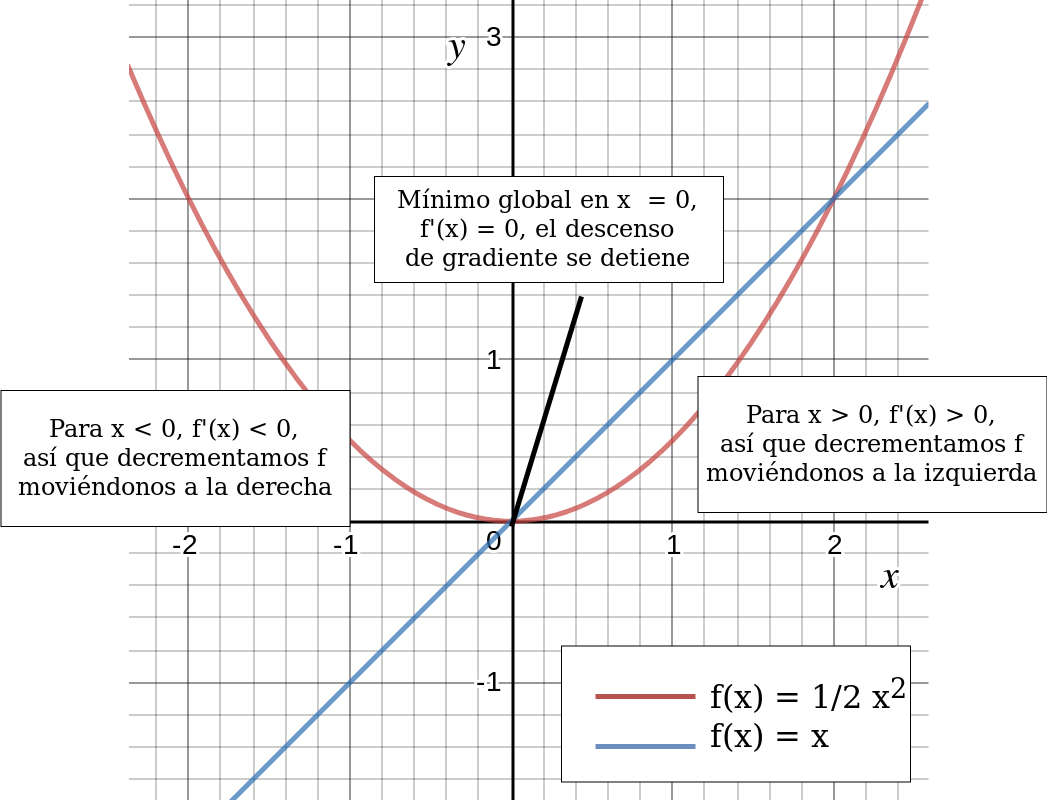
\includegraphics[scale=0.2]{gradient_descent.png}
    \caption{El método del descenso del gradiente utiliza las derivadas de una función para ir cuesta abajo hasta llegar a un mínimo.}
    \label{fig:gradient_descent_first_example}
\end{figure}

Cuando $f'(x) = 0$ la derivada no provee ninguna información sobre la dirección
en la cual moverse. Puntos donde $f'(x) = 0$ se conocen como 
\textit{puntos críticos}. Un \textit{mínimo local} es un punto donde $f(x)$ es
menor que todos sus puntos vecinos, así que no es posible 
disminuir $f(x)$ haciendo pasos infinitesimales. Un \textit{máximo local} es
un punto donde $f(x)$ es mayor que todos los puntos vecinos, así que no es posible
incrementar $f(x)$ con pasos infinitesimales. Algunos puntos críticos no son
ni máximos ni mínimos, son llamados \textit{puntos de silla}.

Un punto que obtiene el valor menor absoluto de $f(x)$ es un \textit{mínimo global}.
Es posible que un mínimo local no sea globalmente óptimo. En el contexto
del aprendizaje profundo, se optimizan funciones que 
pueden tener mínimos locales que no son óptimos, y puntos de silla 
atrapados por regiones planas. Esto hace el proceso de optimización
muy complicado, especialmente si la función es multidimensional.
Por esto, usualmente se busca un valor de $f$ muy bajo, pero
no necesariamente el mínimo en un sentido formal.

Comúnmente se minimizan funciones que tienen múltiples entradas 
$f: \mathbb{R}^n \rightarrow \mathbb{R}$. Para funciones con varias entradas,
se hace uso del concepto de \textit{derivada parcial}. La derivada
parcial $\frac{\partial f(\mathbf{x})}{\partial x_i} $ mide cómo
cambia $f$ cuando sólo la variable $x_i$ se incrementa en el punto $\mathbf{x}$.\\

\begin{remark}
El \textit{gradiente} generaliza la noción de derivada para el caso
donde la derivada es con respecto a un vector: el gradiente de $f$ es el
vector que contiene todas las derivadas parciales, denotado por $\nabla f(\mathbf{x})$. El i-ésimo elemento del gradiente es la 
derivada parcial de $f$ con respecto a $x_i$. En múltiples dimensiones,
los puntos críticos son puntos donde cada elemento del gradiente es igual 
a cero \cite{iangoodfellowyoshuabengioaaroncourville2017}.\\
\end{remark}

\begin{remark}
La \textit{derivada direccional} mide  la tasa de cambio de una función
en un punto sobre un vector. 
La derivada direccional en la dirección $\mathbf{u}$ (un vector
unitario) es la pendiente de la función $f$ en la dirección $\mathbf{u}$ y se denota como $D_\mathbf{u}f(\mathbf{x})$ \cite{iangoodfellowyoshuabengioaaroncourville2017}.
\end{remark}

Para minimizar $f$, nos gustaría encontrar la dirección en la que $f$ disminuye
más rápidamente. Esto se puede hacer a través de la derivada direccional.

\[
\begin{array}{rcl}
            D_\mathbf{u}f(\mathbf{x}) & = & \nabla f(\mathbf{x}) \cdot \mathbf{u}\\
           & = & \|\nabla f(\mathbf{x})\| \|\mathbf{u}\| \cos({\theta})\\
           & = & \|\nabla f(\mathbf{x})\| \cos({\theta})
   \end{array}
\]

se puede ver que el valor máximo de $D_\mathbf{u}f(\mathbf{x})$
se alcanza cuando $\cos({\theta}) = 1$. Por lo tanto $\theta = 0$, y
el valor máximo de la derivada direccional se tiene cuando $\mathbf{u}$
tiene la misma dirección que $\|\nabla f(\mathbf{x})\|$. Este valor
máximo de $D_\mathbf{u}f(\mathbf{x})$ es

\[
\|\nabla f(\mathbf{x})\| \cos({\theta}) = \|\nabla f(\mathbf{x})\| 
\]

De igual forma, el valor mínimo de $D_{\mathbf{u}f(\mathbf{x})}$ puede obtenerse haciendo $\theta  = \pi$ de manera que 
$\mathbf{u}$ apunte a la dirección opuesta de $\nabla f(\mathbf{x})$.\\


\begin{remark}
La derivada direccional $D_\mathbf{u}f(\mathbf{x})$ tiene un valor
máximo $\|\nabla f (\mathbf{\mathbf{x}})\|$
cuando $\mathbf{u}$ tiene la misma dirección que $ \nabla f (\mathbf{x})$ y un mínimo valor $-\|\nabla f (\mathbf{\mathbf{x}})\|$ cuando $\mathbf{u}$ tiene la dirección que $-\nabla f (\mathbf{\mathbf{x}})$. En otras palabras, el vector
gradiente apunta en la dirección de la máxima tasa de crecimiento de la función
y el vector gradiente negativo apunta a la máxima tasa de disminución de la 
función \cite{acourseinmultivariablecalculusanalysis2010}.\\
\end{remark}

\begin{remark}
Podemos disminuir $f$
moviéndonos en la dirección del gradiente negativo. Esto es conocido
como \textit{el método del descenso más empinado} o \textit{descenso del gradiente}.

El descenso del gradiente propone un nuevo punto

\[
\mathbf{x}' = \mathbf{x} - \gamma \nabla f(\mathbf{x})
\]


donde $\gamma$ es la \textit{tasa de aprendizaje}, un escalar positivo
que determina el tamaño de los pasos. Se puede elegir $\gamma$
de diferentes maneras, pero es muy común que $\gamma$
se defina como una constante pequeña.
\end{remark}

El descenso del gradiente converge cuando cada elemento del gradiente es 
cero (en la práctica son valores muy cercanos a cero).

Resumiendo, el método del descenso del gradiente
calcula repetidamente el gradiente $\nabla f(\mathbf{x})$,
y después se mueve en la dirección opuesta. Con ésto, se disminuirá $f$ hasta 
posiblemente alcanzar un mínimo global.

\subsubsection{Terminología}

A continuación se definen diferentes términos que se utilizan a lo
largo del trabajo (las definiciones se obtuvieron de \cite{mehryarmohriafshinrostamizadehameettalwalkar2012}).

\begin{itemize}

\item
  \textbf{Ejemplos o muestras}: objetos o instancias de información usadas para
  aprender o evaluar.
 \item
 \textbf{Características}: El conjunto de atributos, comúnmente representadas
como un vector, asociado a una muestra. 
\item 
\textbf{Etiquetas}: Valores o categorías
asignadas a muestras. 
\item \textbf{Muestra de entrenamiento}: Las muestras usadas
para entrenar un algoritmo. 
\item 
\textbf{Muestra de validación}: Muestras usadas
para ajustar los parámetros de un algoritmo de aprendizaje cuando se
trabaja con datos etiquetados. Los algoritmos de aprendizaje usualmente
tienen uno o más parámetros libres, y la muestra de validación es usada
para seleccionar los valores apropiados para los parámetros del modelo.
\item 
\textbf{Muestra de prueba}: Muestras usadas para evaluar el desempeño de un
algoritmo de aprendizaje. La muestra de prueba está separada del
conjunto de entrenamiento y validación, y no está disponible en la etapa
de aprendizaje. 
\item
\textbf{Función de costo}: También llamada función de error o de pérdida. 
Es una función que mide la
diferencia, o pérdida, entre la etiqueta predicha y la verdadera.
Denotando al conjunto de todas las etiquetas como $Y$ y al conjunto de
todas las posibles predicciones como $Y'$, una función $C$ es una mapeo $C: Y
 \times Y' \rightarrow \mathbb{R}^+$. En la mayoría de los casos $Y = Y'$ y la función
de pérdida está acotada, pero estas condiciones no se cumplen siempre.
Algunos ejemplos comunes de funciones de pérdida incluyen la $0-1$,
definida como $C(y, y') = 1$ si $y \neq y'$ y la pérdida cuadrada definida por
$C(y, y') = (y' - y)^2$. 
\item
\textbf{Conjunto de hipótesis}: Un conjunto de
funciones que mapean características (vectores de características) al
conjunto de etiquetas $Y$. De manera más general, las hipótesis pueden ser
funciones que mapean las características a un conjunto diferente $Y'$.
\end{itemize}



\subsection{Redes neuronales artificiales}


En su forma más general, una \textit{red neuronal artificial} 
o simplemente \textit{red neuronal}, es una máquina diseñada para modelar la manera en la cual el cerebro 
realiza una tarea en particular o una función de interés. Las redes neuronales 
artificiales utilizan
una enorme cantidad de interconexiones de células de cómputo conocidas como neuronas o unidades de procesamiento.\\


\begin{remark}
Una red neuronal artificial es un procesador paralelo distribuido construido de unidades simples de
procesamiento, que tiene una naturaleza propensa a almacenar
conocimiento basado en experiencias y poniéndolo a disposición para su uso. Se 
asemeja al cerebro en dos aspectos:
\begin{enumerate}
    \item El conocimiento es adquirido por la red desde su ambiente a través de un proceso de aprendizaje. El proceso de aprendizaje se hace a través de un algoritmo de aprendizaje.
    \item Las fuerza de conexión entre neuronas, también conocidas como pesos sinápticos, son usadas para almacenar el conocimiento adquirido \cite{johnahertzandersskroghrichardgpalmer1991}.
\end{enumerate}

\end{remark}

En términos generales, una red neuronal artificial consiste de un gran número 
de procesadores simples enlazados por conexiones ponderadas.
Cada unidad recibe entradas que vienen de muchas otras unidades y 
produce un valor escalar como salida que depende sólo de la información
disponible localmente, ya sea de la que guarda internamente o la que llega
a través de las conexiones ponderadas. La información es distribuida 
y actúa como entrada a otras unidades de procesamiento.

Por sí mismo, un elemento de procesamiento no es muy poderoso; el poder
del sistema surge de la combinación de muchas unidades en una red.
Una red está especializada en implementar diferentes funciones cambiando la 
topología de las conexiones en la red y los valores de las
conexiones ponderadas.

Las unidades de procesamiento tienen respuestas como

\begin{equation}\label{eq:neuron-output}
y = f\bigg (\sum_k w_k x_k\bigg )    
\end{equation}

donde $x_k$ son las señales de salida de otros nodos o entradas de un sistema
externo, $w_k$ son los pesos de los enlaces de conexión y $f$ es una función
no lineal. Aquí una la unidad calcula una combinación lineal de los pesos y sus
entradas y la pasa por $f$ para producir un valor escalar. 
$f$ es conocida como \textit{función de activación}, y es muy común que
se utilice una función no lineal acotada y creciente como la sigmoide, definida como sigue

\[
f(u) = \frac{1}{1 + e^{-u}}
\]

\begin{figure}
    \centering
    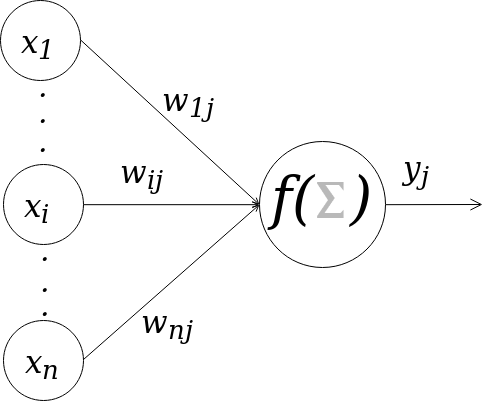
\includegraphics[scale=0.30]{neuron.png}
    \caption{Un modelo de una neurona, la unidad más simple de procesamiento en la red.}
    \label{fig:neuron}
\end{figure}
El término perceptrón a menudo se utiliza para referirse a cualquier
red de nodos \textit{feedforward} con respuestas como la ecuación (\ref{eq:neuron-output}).
Una red puede tener cualquier estructura arbitraria, sin embargo, 
las arquitecturas en capas son muy populares.\\

\begin{remark}
El perceptrón
multicapa o MLP (por sus siglas en inglés), es ampliamente utilizado.
En tales estructuras las unidades en la capa $L$ reciben entradas de la capa
que les precede $L-1$ y envía sus salidas a la capa siguiente $L+1$. Entradas
externas se presentan en la primera capa y las salidas del sistema se toman
de la última capa. Las capas internas se llaman \textit{capas ocultas}. Las redes
más simples tienen una sola capa activa, las de las unidades de salida, por convención, las entradas no se cuentan como una capa activa ya que no realizan
algún tipo de procesamiento. Las redes con una sola capa son menos 
poderosas que las multicapas por lo que sus aplicaciones están
muy limitadas.
\end{remark}

\begin{figure}
    \centering
    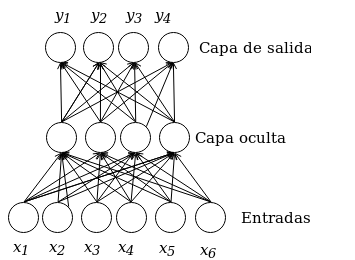
\includegraphics[scale=0.5]{mlp.png}
    \caption{Una red neuronal feedforward completamente conectada con múltiples capas.}
    \label{fig:mpl}
\end{figure}

Que una estructura sea \textit{feedforward} o \textit{prealimentada} significa 
que no existen bucles en la red, la información siempre alimenta
hacia adelante, nunca hacia atrás. La red implementa un
mapeo estático que depende únicamente de las entradas que se presenten y es 
independiente de los estados previos del sistema.\\

\begin{remark}
En una red \textit{completamente conectada}, cada nodo en la capa $L$
recibe entradas de cada nodo en la capa anterior $L-1$ y envía su salida
a todos los nodos en la capa $L+1$.
\end{remark}

Las redes neuronales pueden verse como
gráficas cuyos nodos son unidades de cálculo y cuyas aristas
transmiten información numérica de nodo a nodo. Cada unidad de cómputo es capaz de evaluar su entrada
en una función de activación. La red representa una cadena de funciones compuestas,
que transforman una entrada en un vector de salida. La red es una implementación
particular de una función compuesta desde la entrada hasta el espacio de salida,
a la cual llamamos \textit{función de red}.

En el contexto del aprendizaje automático supervisado,
la experiencia de la que aprenden las redes neuronales es un conjunto 
con patrones de entrada donde cada patrón tiene una salida deseada.
Nuestro problema de aprendizaje consiste
en encontrar la combinación de pesos óptima tal que la función de red 
$\varphi$ se aproxime lo más que se pueda a una función $F$. Sin embargo,
no contamos con la función $F$ explícitamente, sino sólo a través de algunas muestras.

Consideremos una red prealimentada 
con $n$ unidades de entrada y $m$
unidades de salida. Ésta consiste de cualquier número de unidades ocultas
y de cualquier topología en sus conexiones. También contamos
con un conjunto de entrenamiento 
$\{(\mathbf{x}_1, \mathbf{t}_1), \dots, (\mathbf{x}_p, \mathbf{t}_p)\}$, con $p$ pares ordenados de vectores de tamaño $n$ y $m$, los cuales se llaman patrones de entrada y de salida.
Definamos a las funciones de activación de cada nodo en la red como
continuas y diferenciables. Los pesos de las aristas son números reales 
seleccionados aleatoriamente. Cuando el patrón de entrada $\mathbf{x}_i$
del conjunto de entrenamiento se presenta en la red, produce una salida 
$\mathbf{y}_i$, generalmente diferente al objetivo $\mathbf{t}_i$.
Queremos que $\mathbf{y}_i$ y $\mathbf{t}_i$ sean idénticos para
$i = 1, \dots, p$, usando un algoritmo de aprendizaje. De manera
más precisa, queremos minimizar una \textit{función de costo} de la red
con respecto a sus pesos;
por ejemplo la definida como sigue

\[
E = \frac{1}{2} \sum_{i=1}^p \|\mathbf{t}_i - \mathbf{y}_i\|^2
\]


Después de minimizar esta función para el conjunto de entrenamiento, nuevos patrones 
de entrada desconocidos alimentan a la red y esperamos que se interpolen. La red debe reconocer
cuando un nuevo vector de entrada es similar a los patrones aprendidos y producir una salida 
semejante.


El \textit{algoritmo de propagación hacia atrás o retropropagación} es el método
para entrenar redes neuronales más utilizado y se describe en la siguiente sección.

% \subsubsection{Perceptrón}

% El perceptrón es una de las arquitecturas de redes neuronales más simples, inventadas en 1957
% por Frank Rosenblatt.
% Un perceptrón toma varias entradas, $x_1, x_2, \dots$, y produce una salida binaria:

% Imagen

% En el ejemplo se muestra un perceptrón con tres entradas, $x_1, x_2, x_3$. Rosenblatt propuso una regla simple para calcular la salida.
% Introdujo \textit{pesos} ($w_1, w_2, \dots$); número reales que expresan la ``importancia'' de las
% entradas respectivas a la salida. Si la combinación
% lineal de los pesos y las entradas, $\sum_j w_jx_j$ es menor o mayor a un \textit{valor umbral}, la salida de la neurona es ya sea o $0$ o $1$.
% Como los pesos, el umbral es un número real el cual es un parámetro de la neurona. Para ponerlo
% en términos algebraicos más precisos:
% \[
%   salida = 
%   \begin{cases} 
%       0  & \mbox{si } \sum_j w_jx_j \leq umbral\\
%       1  & \mbox{si } \sum_j w_jx_j > umbral 
%   \end{cases}
% \]

% Una forma de ver al perceptrón es como un dispositivo que toma decisiones ponderando evidencia.
% Pongamos el siguiente ejemplo; un festival de música se acerca, te gusta la música y tratas de
% decidir si ir o no al festival. Quieres tomar la decisión tomando en cuenta los siguientes tres 
% factores:

% \begin{itemize}
%     \item ¿Cómo estará el clima?
%     \item ¿Tu mejor amigo o amiga te acompañará?
%     \item ¿Hay medios de transporte públicos cercanos?
% \end{itemize}

% Se pueden representar estos tres factores usando variables binarias $x_1, x_2, x_3$. 
% Por ejemplo,
% $x_1 = 1$ si hay buen clima, y $x_1 = 0$ si hay un mal clima. Similarmente, $x_2 = 1$ si tu amigo
% te irá, y $x_2 = 0$ si no. De igual manera para $x_3$.

% Ahora supón que te encanta la música, y te da igual si tu mejor amigo va o no, 
% o si es difícil llegar al lugar del festival. Pero quizás un mal clima puede arruinar todo.
% Quieres usar perceptrones para modelar este tipo de toma de decisión. Una manera de hacer esto es
% eligiendo los pesos $w_1 = 6$ para el clima, y $w_2 = 2$ y $w_3 = 2$ para las otras condiciones.
% Entre más grande sea el valor de $w_1$ indica que el estado del clima te importa bastante, mucho
% más que si te acompaña tu mejor amigo o si hay medios de transporte públicos cercanos.
% Finalmente, supón que eliges un umbral de $5$ para el perceptrón. Con estas opciones, 
% el perceptrón implementa el modelo de toma de decisión deseado, dando como resultado $1$ cuando
% el clima es bueno, y $0$ cuando es malo. No hay diferencia en la salida cuando tu amigo va o no,
% o si el transporte público está cerca.

% Variando los pesos y el umbral, se pueden obtener diferentes modelos de toma de decisión. 
% Por ejemplo, supongamos que se elige un umbral de $3$. Entonces el perceptrón decidirá que 
% deberías ir al festival cuando el clima es bueno o cuando se cumple que tu mejor amigo o amiga
% irá y hay un medio de transporte público cercano. En otras palabras, se tiene otro modelo de toma
% de decisiones. Minimizar el valor del umbral significa que estás más dispuesto a ir al festival.

% Lo que el ejemplo ilustra es como un perceptrón puede ponderar diferentes tipos de evidencia para
% tomar decisiones. Y parece plausible que una compleja red de perceptrones pueda tomar decisiones 
% más complicadas:


% Imagen de muchos perceptrones conectados

% En esta red, la primera columna de perceptrones, que llamaremos \textit{capa} de perceptrones,
% toma tres simples decisiones, ponderando la evidencia en la entrada. En la segunda capa cada uno
% de esos perceptrones está tomando decisiones ponderando los resultados de la primera capa.
% De esta manera, un perceptrón en la segunda capa, puede tomar una decisión de un nivel más
% complejo y abstracto que los de la primera capa. Incluso se pueden tomar decisiones mucho más
% complejas por el perceptrón de la tercera capa.
% De este modo, una red de perceptrones de múltiples capas puede realizar una toma de decisiones
% más sofisticada.

% Simplifiquemos la manera en que se describen los perceptrones. El primer cambio es escribir 
% $\sum_j w_jx_j$ como un producto punto, $\mathbf{w} \cdot \mathbf{x} = \sum_j w_jx_j$, donde
% $\mathbf{w}$ y $\mathbf{x}$ son los vectores cuyos componentes son los pesos y las entradas,
% respectivamente. El segundo cambio es mover al umbral del otro lado de la desigualdad, y
% reemplazarlo por lo que se conoce como el \textit{sesgo del perceptrón}, $b = -umbral$. Usando
% este sesgo en vez del umbral, la representación de la regla del perceptrón puede ser rescrita como:

% \[
%   salida = 
%   \begin{cases} 
%       0  & \mbox{si } \mathbf{w} \cdot \mathbf{x} + b \leq 0\\
%       1  & \mbox{si } \mathbf{w} \cdot \mathbf{x} + b > 0 
      
%   \end{cases}
% \]

% Se puede ver al sesgo como una medida de qué tan fácil es para el perceptrón producir en su salida
% $1$. Para un perceptrón con un sesgo muy grande, es muy fácil que la salida sea $1$. Pero si el sesgo
% es muy negativo, entonces es muy difícil que la salida del perceptrón sea $1$. 

% El perceptrón puede actualizar automáticamente los pesos y sesgos a través de un algoritmo de
% aprendizaje.

% \subsubsection{Neuronas sigmoides}

% Así como los perceptrones, la neurona sigmoide tiene entradas, $x_1, x_2, \dots$, pesos
% para cada entrada $w_1, w_2, \dots$, y un sesgo, $b$. Pero la salida no es $0$ o $1$. En vez de esto,
% es $s(\mathbf{w \cdot x} + b)$, donde $sigma$ es llamada la función sigmoide, y está definida por:
% \[
% s(z) = \frac{1}{1+e^{-z}}
% \]

% De manera más explícita, la salida de la neurona sigmoide con entradas $x_1, x_2, \dots$, pesos
% $w_1, w_2,\dots$ y el sesgo $b$ es:

% \[
% \frac{1}{1 + \exp(-\sum_{j}w_jx_j - b)}
% \]

% La función sigmoide produce resultados similares a una función escalonada en la que la
% salida está entre $0$ y $1$. La curva cruza $0.5$ cuando $z=0$, lo que puede establecer las reglas
% para una función escalonada como la del perceptrón: 
% si la salida de la neurona sigmoide es mayor
% o igual a $0.5$, produce $1$, si la salida es menor a $0.5$ entonces el resultado es $1$.
% Si $z$ es muy negativa, entonces la salida es aproximadamente $0$; si $z$ es muy positiva, la salida
% es aproximadamente $1$. 

% Con todo lo anterior se puede ver que si $s$ fuera una función escalonada, la neurona sigmoide
% sería un perceptrón. Sin embargo, el factor principal que diferencia a los perceptrones 
% de las neuronas sigmoides, es la suavidad de esta última. 
% La función sigmoide es suave y tiene una derivada muy simple $s(z) (1 - s(z))$, la cual
% es diferenciable en cualquier punto.
% La suavidad en $s$ implica que
% pequeños cambios en los pesos, $\Delta w_j$, y en el sesgo,
% $\Delta b$, produzcan un pequeño cambio en la salida
% $\Delta salida$.
% Por último cabe señalar que la salida de las neuronas en general
% no necesariamente debe ser una función sigmoide, en ocasiones
% se consideran neuronas con salida $f(\mathbf{w \cdot x} + b)$
% para alguna \textit{función de activación} $f(\cdot)$. 


% \subsubsection{Arquitectura de las redes neuronales}

% Una red puede tener una estructura arbitraria, pero
% las arquitecturas con capas son las más populares.
% Supongamos que tenemos la siguiente red:

% Imagen

% La capa de más a la izquierda en la red es llamada capa de entrada,
% y las neuronas dentro de la capa son llamadas
% \textit{neuronas de entrada}. La capa de más a la derecha o capa 
% de salida contiene a las \textit{neuronas de salida}, o, en este 
% caso, una sola neurona de salida. La capa interna se conoce como
% \textit{capa oculta}. La red de la Figura tiene sólo
% una capa oculta, pero algunas redes cuentan con múltiples capas
% ocultas. Por ejemplo la siguiente tiene dos capas ocultas:


% A veces a estas redes se les conoce como perceptrones de
% múltiples capas o MLP (por sus siglas en inglés), a pesar de estar compuestas por 
% neuronas sigmoides o por neuronas con otras funciones de activación y no por perceptrones.

% La red de la Figura tiene una estructura donde la salida de una
% capa es la entrada de la siguiente capa. Tales redes se llaman
% \textit{red neuronales prealimentadas}. Lo que esto significa es
% que no existen bucles en la red, la información siempre alimenta
% hacia adelante, nunca hacia atrás. 

\subsubsection{Retropropagación}

% Las redes neuronales abarcadas hasta ahora pueden verse como
% gráficas cuyos nodos son unidades de cálculo y cuyas aristas
% transmiten información numérica de nodo a nodo. Cada unidad de cómputo es capaz de evaluar su entrada
% en una función de activación. En realidad, la red representa una cadena de funciones compuestas,
% que transforman una entrada en un vector de salida. La red es una implementación
% particular de una función compuesta desde la entrada hasta el espacio de salida, a la cual
% llamamos \textit{función de red}. El problema de aprendizaje consiste
% en encontrar la combinación de pesos óptima tal que la función de red 
% $\varphi$ se aproxime lo más que se pueda a una función $f$. Sin embargo,
% no contamos con la función $f$ explícitamente, sino sólo a través de algunas muestras.

% Consideremos una red prealimentada 
% con $n$ unidades de entrada y $m$
% unidades de salida. Ésta consiste de cualquier número de unidades ocultas
% y de cualquier patrón de conexiones (hacia adelante). También contamos
% con un conjunto de entrenamiento 
% $\{(\mathbf{x}_1, \mathbf{t}_1), \dots, (\mathbf{x}_p, \mathbf{t}_p)\}$, con $p$ pares ordenados de vectores de tamaño $n$ y $m$, los cuales se llaman patrones de entrada y de salida.
% Definamos a las funciones de activación de cada nodo en la red como
% continuas y diferenciables. Los pesos de las aristas son números reales 
% seleccionados aleatoriamente. Cuando el patrón de entrada $\mathbf{x}_i$
% del conjunto de entrenamiento se presenta en la red, produce una salida 
% $\mathbf{o}_i$, generalmente diferente al objetivo $\mathbf{t}_i$.
% Queremos que $\mathbf{o}_i$ y $\mathbf{t}_i$ sean idénticos para
% $i = 1, \dots, p$, usando un algoritmo de aprendizaje. De manera
% más precisa, queremos minimizar una \textit{función de costo} (también
% denominada como de error o pérdida) de la red;
% por ejemplo la definida como sigue:

% \[
% E = \frac{1}{2} \sum_{i=1}^p \|\mathbf{t}_i - \mathbf{o}_i\|^2
% \]


% Después de minimizar esta función para el conjunto de entrenamiento, nuevos patrones 
% de entrada desconocidos alimentan a la red y esperamos que se interpolen. La red debe reconocer
% cuando un nuevo vector de entrada es similar a los patrones aprendidos y producir una salida 
% semejante.

% El \textit{algoritmo de propagación hacia atrás o retropropagación} es el método
% para entrenar redes neuronales más utilizado.
El término retropropagación se refiere a dos cosas diferentes. Primero,
describe un método para calcular las derivadas de la función de costo con respecto
a los pesos aplicando la regla de la cadena. Segundo, describe un algoritmo
de entrenamiento, equivalente al descenso del gradiente; el gradiente de la función
de costo es calculado y usado para corregir los pesos iniciales, que fueron 
elegidos aleatoriamente.

Como algoritmo de entrenamiento, el propósito de la retropropagación es ajustar
los pesos de la red para producir la salida deseada como resultado 
a cada patrón de entrada un un conjunto de patrones de entrenamiento.
Es un algoritmo \textit{supervisado} en el sentido que, para cada
patrón de entrada, existe exactamente una salida correcta.

Para entrenar una red, es necesario tener un conjunto de patrones de
entrada y sus salidas deseadas correspondientes, además una función
de error que mide el ``costo'' de las diferencias entre las salidas 
de la red y los valores deseados. De manera muy general,
los pasos básicos del algoritmo son los siguientes:

\begin{enumerate}
    \item Inicializar los pesos de manera aleatoria con valores pequeños.
    \item Alimentar a la red con una muestra del conjunto de entrenamiento para obtener las salidas. Este paso 
    también es conocido como feedforward o propagación hacia adelante.
    \item Comparar las salidas con los valores deseados y calcular el error.
    \item Calcular las derivadas del error con respecto a cada uno de los pesos $\frac{\partial E}{\partial w_{ij}}$.
    \item Ajustar los pesos para minimizar el error.
    \item Repetir.
\end{enumerate}


% A continuación se describen los pasos del algoritmo después del paso de inicialización
% aleatoria de los pesos.


\paragraph{Propagación hacia adelante}
Por simplicidad, supongamos que los nodos están indexados tal que $i < j$ implica que 
el nodo $j$ sigue al nodo $i$ en términos de dependencia. Esto quiere decir que,
el estado del nodo $j$ puede depender, quizás indirectamente, del estado 
del nodo $i$, pero el nodo $i$ no depende del nodo $j$. Esta notación permite que durante
las simulaciones se evite la necesidad de lidiar con cada capa de manera separada,
al hacer un seguimiento de los índices de la capa. Por supuesto, este esquema de
indexado es compatible con las estructuras multicapas.

En el paso hacia adelante, la red calcula una salida basada en sus entradas actuales. Cada nodo
$j$ calcula una suma ponderada $a_j$ de sus entradas y la pasa a través de una función
para obtener la salida del nodo $y_j$.

\begin{equation}\label{linear_combination_aj}
a_j = \sum_{i < j} w_{ij} y_i    
\end{equation}


\begin{equation}
y_j = f(a_j)    
\end{equation}


$w_{ij}$ denota el peso que llega al nodo $j$ desde el nodo $i$. El índice $i$ en la suma
va sobre todos los índices $i < j$ de nodos que envían una entrada al nodo $j$. Normalmente
la función $f$ es la sigmoide, sin embargo, no es la única función de activación.
% Es importante mencionar que 
% asumiremos que existen nodos de sesgos con una salida constante igual a $1$,
% para evitar darle un manejo especial a los pesos de los sesgos. 

Cada nodo es evaluado en orden, comenzando con el primer nodo oculto
y continuando hasta llegar al último nodo de salida. En 
redes con múltiples capas, la primera capa oculta se actualiza basándose en las
salidas de los nodos de entrada, que son los valores de un vector de características 
de una muestra; la segunda capa oculta se actualiza basándose en las
salidas de la primera capa oculta, y se continúa así hasta llegar a la capa de salida
la cual se actualiza con las salidas de la última capa oculta.




% Consideremos primero una red con dos capas como la de la Figura. La notación que usaremos 
% se muestran en la Figura; las unidades de salida están denotadas por $o_i$, las
% unidades de la capa oculta por $v_{j}$ y las de entrada por $x_{k}$. Hay aristas con pesos
% $w_{jk}$ de los nodos de entrada a los nodos ocultos, y $w_{ij}$ de las unidades ocultas a las
% unidades de salida. Es importante destacar que el índice $i$ siempre se refiere a un unidad
% de salida, $j$ a una oculta y $k$ a una entrada.

% Por ahora el entrenamiento se realiza con un solo patrón del conjunto de entrenamiento,
% para evitar el exceso de índices, por lo tanto $p = 1$. Más adelante se explica el caso con 
% más muestras, $p > 1$.


% Dado un patrón, la unidad oculta $j$ recibe la suma ponderada de las entradas

% \[
% h_j = \sum_k w_{jk} x_k
% \]

% y produce una salida 

% \[
% v_{j} = g(h_j) = g(\sum_k w_{jk} x_k).
% \]

% La unidad de salida $i$ por tanto recibe

% \[
% h_{i} = \sum_j w_{ij} v_j = \sum_j w_{ij}g(\sum_k w_{jk} x_k)
% \]

% y produce la salida final 

% \[
% o_i = g(h_i) = g(\sum_j w_{ij} v_j) = g(\sum_j w_{ij}g(\sum_k w_{jk} x_k))
% \]


% Normalmente $g$ es la función sigmoide, sin embargo, existen otras funciones
% de activación. 

\paragraph{Cálculo del error}
A menos que la red esté perfectamente entrenada, las salidas de la red diferirán de
las salidas deseadas. Como ya vimos, para medir esa diferencia, se utiliza una función de costo, 
que por ahora será la \textit{suma de cuadrados del error} o \textit{SSE} (por sus 
siglas en inglés).

\[
E = \frac{1}{2} \sum_p\sum_k(t_{pk} - y_{pk})^2
\]

donde $p$ indexa a todos los patrones del conjunto de entrenamiento, $k$ indexa a
los nodos de salida, $t_{pk}$ y $y_{pk}$ son respectivamente, el objetivo y la salida actual de la red para el
$k$ ésimo nodo de salida de la muestra $p$.
Una de las razones por las que la SSE es conveniente es porque los errores entre las diferentes
muestras o patrones y las diferentes salidas son independientes, el error
total es la suma de los errores cuadrados individuales.

\[
E = \sum_p E_p
\]
donde 
\[
E_p = \frac{1}{2} \sum_k (t_{pk} - y_{pk})^2
\]

\paragraph{Cálculo de las derivadas}
Después de obtener las salidas y de haber calculado el error, el siguiente paso es
calcular la derivada del error con respecto de los pesos. Recordando que $E = \sum_p E_p$
es la suma del error individual de los patrones, entonces la derivada total
es sola la suma de las derivadas por muestra.

\[
\frac{\partial E}{\partial w_{ij}} = \sum_p \frac{\partial E_p}{\partial w_{ij}}.    
\]


Lo que hace eficiente a la retropropagación (el cálculo de la derivada) es cómo se descompone la operación 
y el orden de los pasos. 

Conviene calcular de forma separada las derivadas del error
con respecto a los pesos que se conectan a la unidad de salida
y para las conexiones de los nodos ocultos.

La derivada con respecto a las conexiones a las unidades de salida puede ser escrita como

\begin{equation}\label{eq:derivative-output}
    \frac{\partial E_p}{\partial w_{jk}} = \frac{\partial E_p}{\partial y_k}\frac{\partial y_k}{\partial a_k} \frac{\partial a_{k}}{\partial w_{jk}}
\end{equation}

donde $k$ indexa a una unidad de salida y $a_k$ se calcula
utilizando la ecuación \ref{linear_combination_aj}. Conviene primero calcular un valor
$\delta_k$ para cada nodo de salida $k$. Este valor delta también es conocido
como \textit{error de retropropagación}.

\begin{align*}
\delta_k &= \frac{\partial E_p}{\partial y_k}\frac{\partial y_k}{\partial a_k} \\
&= -(t_k - y_k) f'(a_k).
\end{align*}

Para el tercer término de (\ref{eq:derivative-output}), 
como $a_k$ es una suma lineal, es cero si $i \neq j$, de otra forma
\begin{align*}
    \frac{\partial a_k}{\partial w_{jk}} &=  \frac{\partial \sum_i w_{ik}y_i}{\partial w_{jk}}\\
    &= y_j.
\end{align*}
Por lo tanto
\begin{align*}
    \frac{\partial E_p}{\partial w_{jk}} = \delta_k y_j 
\end{align*}

El segundo caso corresponde al cálculo de las derivadas con respecto a los
pesos que se conectan a unidades ocultas. El cálculo de la derivada hasta estos pesos
no se obtiene de manera directa, como el caso de las conexiones a las unidades de salida,
por lo que la derivada se obtiene calculando

\begin{align*}
    \frac{\partial E_p}{ \partial w_{ij}} = \sum_k \frac{\partial E_p}{\partial y_k} \frac{\partial y_k}{\partial a_k} \frac{\partial a_k}{\partial y_j} \frac{\partial y_j}{\partial a_j} \frac{\partial a_j}{\partial w_{ij}}
\end{align*}

donde $k$ indexa a todas los nodos a los que se conecta la unidad $j$, por ahora suponemos 
que son las $k$ unidades de salida. Simplificando la expresión, podemos ver que
en los primeros dos factores de la suma estamos calculando los valores delta de las unidades de 
salida, de ahí el nombre de error de retropropagación.

\begin{align*}
    \frac{\partial E_p}{ \partial w_{ij}} &= \sum_k \frac{\partial E_p}{\partial a_k} \frac{\partial a_k}{\partial y_j} \frac{\partial y_j}{\partial a_j} \frac{\partial a_j}{\partial w_{ij}}\\
    &= \sum_k \delta_k w_{jk} \frac{\partial y_j}{\partial a_j} \frac{\partial a_j}{\partial w_{ij}} \\
    &= \sum_k \delta_k w_{jk} f'(a_j) \frac{\partial a_j}{\partial w_{ij}} \\
    &= \delta_j y_i
\end{align*}

donde $\delta_j = \sum_k \delta_k w_{jk} f'(a_j)$. De manera general
para calcular la derivada de la función de costo con respecto a cualquiera de
los pesos tenemos

\[
\frac{\partial E_p}{\partial w_{ij}} = \delta_j y_i
\]

donde $\delta_j$ es el error de retroprogación de la unidad $j$, que es
a la unidad a la que llega la arista con el peso $w_{ij}$ y $y_i$ 
es la salida de la unidad $i$ que será la entrada del nodo $j$.


% El término $f'(a_{pk})$ es la pendiente de la función de activación evaluada
% en el punto $a_{pk}$. La función sigmoide es conveniente porque $f'$ es una 
% función simple de la salida del nodo: $f'(a_{pk}) = y(1-y)$, donde $y = f(a_{pk})$.


% \begin{equation}\label{eq:derivative_from_weigths}
% \frac{\partial E_p}{\partial w_{ij}} = \sum_k \frac{\partial E_p}{\partial a_k} \frac{\partial a_k}{\partial w_{ij}}
% \end{equation}

% donde el índice $k$ recorre todos los nodos de salida y $a_i$ es la suma ponderada de la entrada
% para el nodo $i$. Es conveniente primero calcular un valor $\delta_j$ para cada nodo $j$

% \begin{align*}
%     \delta_j &= \frac{\partial E_p}{\partial a_j} \\
%              &= \frac{\partial E_p}{\partial y_j} \frac{\partial y_j}{\partial a_j}
% \end{align*}

% que mide la contribución de $a_j$ al error del patrón actual.

% Para las unidades de salida, $\frac{\partial E_p}{\partial a_k}$ se obtiene directamente

% \begin{align*}
% \delta_k &= \frac{\partial E_p}{ \partial y_{pk}}\frac{\partial y_{pk}}{ \partial a_{pk}} \\
%          &= \frac{\partial \frac{1}{2} \sum_k (t_{pk} - y_{pk})^2}{\partial y_{pk}}
%          \frac{\partial f(a_{pk})}{ \partial a_{pk}}\\
%          &= - (t_{pk} - y_{pk}) f'(a_{pk}). 
% \end{align*}

% El término $f'(a_{pk})$ es la pendiente de la función de activación evaluada
% en el punto $a_{pk}$. La función sigmoide es conveniente porque $f'$ es una 
% función simple de la salida del nodo: $f'(a_{pk}) = y(1-y)$, donde $y = f(a_{pk})$.

% Para los nodos ocultos, $\delta_j$ se obtiene de manera indirecta. Los nodos ocultos pueden influir 
% al error sólo a través de su efecto en los nodos $k$ a los que envía sus conexiones de salida

% \begin{align*}
%     \delta_j &= \frac{\partial E_p}{\partial a_j} \\
%     &= \sum_k \frac{\partial E_p}{\partial a_k} \frac{\partial a_k}{\partial a_j}.
% \end{align*}

% Se puede ver que el primer término es $\delta_k$ del nodo $k$ por lo que se tiene

% \[
% \delta_j = \sum_k \delta_k \frac{\partial a_k}{\delta a_j}
% \]


% El segundo factor se obtiene de la siguiente manera

% \begin{align*}
%     \frac{\partial a_k}{\delta a_j} &= \frac{\partial \sum_{i < k} w_{jk} f(a_i)}{\partial a_j}\\
%     &= \frac{ \partial (w_{1k} f(a_1) + w_{2k} f(a_2) + \dots + w_{jk} f(a_i) + \dots) }{\partial a_j}\\
%     &= 0 + 0 + \dots + w_{jk} f'(a_j) + 0 \dots
% \end{align*}

% con esto tenemos

% \[
% \delta_j = f'_j \sum_k w_{jk} \delta_k.
% \]

% $\delta_j$ es la suma ponderada de los valores $\delta_k$ de los nodos $k$
% a los que tiene conexiones con pesos $w_{jk}$.

% Porque $\delta_k$ debe ser calculada antes que $\delta_j$, $j < k$,
% el procesos comienza de las unidades de salida hasta llegar a las 
% entradas, por eso el nombre de retropropagación. Primero los
% valores $\delta$ de los nodos de salida se calculan, después los valores
% son calculados para los nodos que están conectados a las salidas, luego
% los valores son calculados para los nodos que estén a dos capas de las 
% salidas y así para los siguientes.

% Resumiendo, hasta ahora tenemos

% \[
%   \delta_j = 
%   \begin{cases} 
%       -(t_{pj}-y_{pj})f'_j              & \mbox{para los nodos de salida}   \\
%       f'_j\sum_k w_{jk}\delta_k & \mbox{para los nodos ocultos}
%   \end{cases}
% \]

% Para los nodos de salida, $\delta_j$ sólo depende del error $(t_j - y_j)$ y la
% pendiente $f'_j$ de su función de activación. Para los nodos ocultos,
% $\delta_j$ es la suma ponderada de los $\delta$ de todos los nodos
% a los que envía su salida, multiplicada por su propia pendiente $f'_j$. 
% En redes con múltiples capas, los valores delta primero
% son evaluados en los nodos de salida basándose en los errores
% del patrón actual, la última capa oculta se evalúa entonces basándose
% en los valores delta de la salida, la penúltima capa oculta se actualiza de
% acuerdo a los valores de la última capa oculta, y así hacia atrás
% hasta llegar a la capa de entrada. Normalmente no es necesario calcular
% valores delta para la capa de entrada, así que el proceso se detiene
% con la primera capa oculta.

% Habiendo obtenido los deltas, es fácil encontrar las derivadas parciales
% $\frac{\partial E_p}{w}$ con respecto de los pesos. El segundo término en 
% la ecuación \ref{eq:derivative_from_weigths} es $\frac{\partial a_j}{\partial w_{ij}}$.
% Como $a_k$ es una suma lineal, es cero si $k \neq j$, de otra forma

% \[
% \frac{\partial a_j}{\partial w_{ij}} = y_i
% \]

% donde $y_i$ es la salida del nodo $i$. Finalmente de \ref{eq:derivative_from_weigths}
% la derivada del error del patrón $p$, $E_p$, con respecto al peso $w_{ij}$ es entonces

% \begin{equation}\label{eq:p_error_with_respect_to_weight}
%     \frac{\partial E_p}{\partial w_{ij}} = \delta_j y_i
% \end{equation}

% el producto del valor delta del nodo $j$ y la salida del nodo $i$.
\begin{figure}
    \centering
    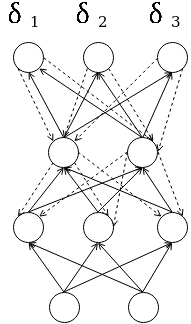
\includegraphics[scale=0.5]{backprop.png}
    \caption{La retropropagación en una red de tres capas. Las líneas sólidas muestran el paso
    del feedforward y las líneas discontinuas muestras la propagación hacia atrás de los valores $\delta$.}
    \label{fig:backprop}
\end{figure}
\paragraph{Actualización de los pesos}
Después de obtener las derivadas, el siguiente paso es actualizar los pesos
para disminuir el error. Como se dijo al principio, el término 
de retropropagación se refiere al método eficiente para calcular las 
derivadas $\frac{\partial E}{\partial w}$ y al algoritmo de optimización
que utiliza esas derivadas para ajustar los pesos y reducir el error.

La retropropagación como método de optimización es básicamente el 
descenso del gradiente. Sabemos que el gradiente negativo de $E$ apunta a la
dirección en la que $E$ se decrementa más rápido. Para minimizar $E$,
los pesos son ajustados en la dirección del gradiente negativo. La regla para
actualizar los pesos es

\[
w_{ij} \leftarrow  w_{ij} - \gamma \frac{\partial E}{\partial w_{ij}}
\]

donde la \textit{tasa de aprendizaje} $0 < \gamma$.
Hay dos variaciones básicas para la actualización, el \textit{modo por lotes} y 
\textit{en línea}.

\begin{itemize}
    \item \textbf{Aprendizaje por lotes}: En este modo, cada patrón $p$ es evaluado para obtener los términos de la derivada $\frac{\partial E_p}{\partial w}$; estos se suman para obtener la derivada total
    \[
      \frac{\partial E}{\partial w}  = \sum_p \frac{\partial E_p}{\partial w} 
    \]
    y sólo después de esto se actualizan los pesos. Los pasos son los siguientes:
    
    \begin{enumerate}
        \item Por cada patrón $p$ en el conjunto de entrenamiento
            \begin{itemize}
                \item Alimentar a la red con el patrón $p$ y hacer la propagación hacia adelante para obtener la salidas de la red.
                \item Calcular el error del patrón $E_p$ y retropropagar para obtener 
                las derivadas por patrón $\frac{\partial E_p}{\partial w}$.
            \end{itemize}
        \item Sumar todas las derivadas por patrón para obtener la derivada total.
        \item Actualizar los pesos
        \[
            w \leftarrow w - \gamma \frac{\partial E}{\partial w}
        \]
        \item Repetir.
    \end{enumerate}
    
    Cada paso a través de todo el conjunto de entrenamiento se llama \textit{época}.
    
    \item \textbf{Aprendizaje en línea}: En este modo de aprendizaje, los pesos
    se actualizan después de que se presenta cada patrón. Generalmente, un patrón $p$ se
    elige aleatoriamente y se presenta a la red. La salida se compara con el objetivo
    para ese patrón y los errores son propagados hacia atrás para obtener una
    derivada $\frac{\partial E_p}{\partial w}$  para un solo patrón. Los pesos se actualizan
    inmediatamente después, usando el gradiente del error de un solo patrón.
    Los pasos son:
    
    \begin{enumerate}
        \item Elegir aleatoriamente un patrón $p$ del conjunto de entrenamiento.
        \begin{itemize}
            \item Alimentar a la red con el patrón $p$ y propagar hacia adelante para
            obtener las salidas de la red.
            \item Calcular el error $E_p$ y retropropagar para obtener las derivadas $\frac{\partial E_p}{\partial w}$.
        \end{itemize}
        \item Actualizar los pesos usando la derivada de un solo patrón
        \[
            w \leftarrow w- \gamma \frac{\partial E_p}{\partial w}
        \]
        \item Repetir.
    \end{enumerate}
\end{itemize}


% Conviene primero calcular un valor $\delta_r$ para cada nodo $r$.

% \[
% \delta_r = \frac{\partial E_p}{ \partial h_r}
% \]

% La derivada para las aristas que conectan a las unidades ocultas y las de salida
% puede ser escrita como

% \begin{align*}\label{eq:hidden-output-derivative}
%     \frac{\partial E}{\partial w_{ij}} & = \frac{\partial E}{\partial o_i} \frac{\partial o_i}{\partial w_{ij}} \\
%     & =- (t_i - o_i) g'(h_i) v_j \\
%     & = \delta_i v_j
% \end{align*}

% definidos a  $\delta_i = -g'(h_i)(t_i - o_i)$.





% \subsubsection{El caso de redes con múltiples capas}


\subsubsection{Retropropagación en una forma matricial}

En estructuras de redes prealimentadas con múltiples capas, es conveniente 
reescribir el método de retropropagación en una forma
tal que las operaciones se simplifiquen a multiplicaciones
de vectores por matrices, matrices por vectores, matrices por matrices y vectores por vectores.
A continuación definiremos una red con dos capas, una oculta y una de salida, sin embargo,
se puede ver que es posible generalizar para redes con más capas ocultas. Todas las operaciones que se realizan son con respecto a una muestra $p$, por lo que
dependiendo de cómo se realice la actualización de los pesos, es como se
deben de realizar las operaciones con las matrices de las derivadas que obtendremos al final.


Consideraremos una red con $n$ unidades de entrada, $k$ unidades ocultas y $m$ unidades de salida. 
Hasta ahora la notación utilizada ha evitado que tratemos cada capa de una red
por separado, pero ahora es necesario mantener un índice de la capa sobre la que
se están haciendo los cálculo, por lo tanto se usa el superíndice $(l)$ para referirnos
a la capa $l$.
Los pesos entre la unidad de entrada $i$ y la oculta $j$ se denotan por $w_{ij}^{(1)}$. El peso 
entre la unidad oculta $i$ y la de salida $j$ será $w_{ij}^{(2)}$.

% El sesgo $b$ de cada unidad
% está implementado como el peso de una arista adicional. Por lo tanto, los vectores de entrada
% se extienden con un componente $1$, y lo mismo para el vector de salida de la capa oculta. 
% El peso entre la constante $1$ y la unidad oculta $j$ se llama $w_{n+1,j}^{(1)}$ y el peso
% entre la constante $1$ y la unidad de salida $j$ se denota por $w_{k+1, j}^{(2)}$.


Existen $n \times k$ pesos entre las unidades de entrada y las ocultas y
$k \times m$ entre las ocultas y las de salida. Sea $\mathbf{W_1}$ la matriz de
tamaño $n \times k$ cuyo componente $w_{ij}^{(1)}$ está en la $i$ ésima
fila y la $j$ ésima columna. De manera similar definamos $\mathbf{W}_2$ 
como la matriz de $k \times m$ con elementos $w_{ij}^{(2)}$. 
El vector de entrada es de tamaño $n$,  y lo definimos como $\mathbf{x} = (x_1, \dots, x_n)$. 

\begin{figure}
    \centering
    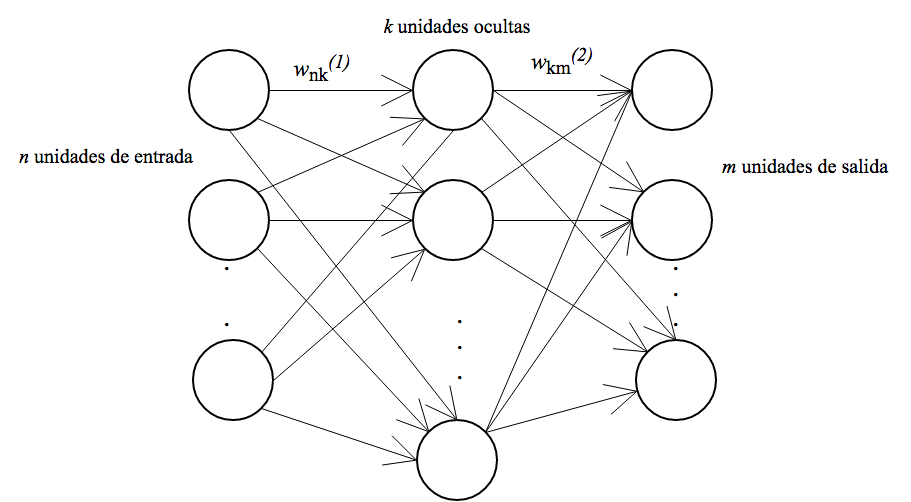
\includegraphics[scale=0.3]{mat_struct.png}
    \caption{Arquitectura de la red propuesta para la notación matricial de la retropropagación.}
    \label{fig:mat_mult_struct}
\end{figure}

Por ahora como función de activación usaremos a la sigmoide, por lo que la salida $y_j^{(1)}$ de la
unidad es

\[
y_j^{(1)} = f(\sum_{i}^{n} w_{ij}^{(1)}x_i) = \frac{1}{1+e^{\sum_{i}^{n} w_{ij}^{(1)}x_i}}
\]
 
Las salidas de la capa oculta se pueden obtener aplicando la función de activación a cada uno de los
elementos que resulten de la multiplicación
$\mathbf{x}\mathbf{W}_1$. El vector $\mathbf{y}^{(1)}$ cuyos componentes son las salidas de las unidades
ocultas está dado por

\[
\mathbf{y}^{(1)} = f(\mathbf{x}\mathbf{W}_1).
\]
Las salidas de las unidades en la capa de salida se calculan
usando el vector $\mathbf{y}^{(1)} = (y_1^{(1)},\dots, y_k^{(1)})$. La salida de la 
red es un vector $m$ dimensional $\mathbf{y}^{(2)}$, donde

\[
\mathbf{y}^{(2)} = f(\mathbf{y}^{(1)}\mathbf{W}_2).
\]

En el paso de feedforward, el vector $\mathbf{x}$ alimenta a la red.
Los vectores $\mathbf{y}^{(1)}$ y $\mathbf{y}^{(2)}$ son calculados.
Además, en este paso se pueden obtener las derivadas evaluadas 
de las funciones de activación, que se pueden escribir en matrices diagonales $\mathbf{D}_l$. Para nuestra red de dos capas,
$\mathbf{D}_2$ contiene las derivadas evaluadas de las funciones
de activación de los nodos de salida, y $\mathbf{D}_1$ para
las unidades ocultas. Por simplicidad, supusimos que $f$ es la sigmoide
y por lo tanto las derivadas son $f' = y(1-y)$.

\[
\mathbf{D}_2 = 
\begin{pmatrix}
    y_1^{(2)}(1-y_1^{(2)}) & 0 & \dots & 0 \\
    0 & y_2^{(2)}(1- y_2^{(2)}) & \dots & 0 \\
    \vdots & \vdots & \ddots & \vdots\\
    0 & 0 & \dots & y_m^{(2)}(1-y_m^{(2)}))
\end{pmatrix}
\]   
y


\[
\mathbf{D}_1 = 
\begin{pmatrix}
    y_1^{(1)}(1 - y_1^{(1)}) & 0 & \dots & 0 \\
    0 & y_2^{(1)}(1 - y_2^{(1)}) & \dots & 0 \\
    \vdots & \vdots & \ddots & \vdots\\
    0 & 0 & \dots & y_k^{(1)}(1 - y_k^{(1)}))
\end{pmatrix}
\]

Para calcular los valores delta de la unidad de salida
necesitamos las derivadas del error con respecto a las salidas. 
Definimos al vector $\mathbf{e}$ con las derivadas de las desviaciones cuadráticas como

\[
\mathbf{e} = 
\begin{pmatrix}
    - (t_1 - y_1^{(2)}) \\
    - (t_2 - y_2^{(2)}) \\
    \vdots \\
    - (t_m - y_m^{(2)})
\end{pmatrix}
\]

Para una unidad de salida  $\delta_i^{(2)} = - (t_i - y_i^{(2)})y_i^{(2)}(1- y_i^{(2)})$. Por lo tanto
el vector $m$ dimensional $\boldsymbol{\delta^{(2)}}$ que contiene todos los
valores delta de la unidad de salida está dado por

\[
\boldsymbol{\delta}^{(2)} = \mathbf{D}_2\mathbf{e}.
\]



El vector de tamaño $k$ de valores delta en la capa oculta es
\[
\boldsymbol{\delta}^{(1)} = \mathbf{D}_1\mathbf{W}_2 \boldsymbol{\delta}^{(2)}.
\]

Después de calcular los vectores con los valores delta, es posible
obtener las derivadas del error con respecto a los pesos.
Las matrices con las derivadas del error con respecto los pesos de $\mathbf{W}_2$
y $\mathbf{W}_1$, son respectivamente:

\[
\nabla \mathbf{W}_2 = (\boldsymbol{\delta}^{(2)}\mathbf{y}^{(1)})^T
\]
\[
\nabla \mathbf{W}_1 = (\boldsymbol{\delta}^{(1)}\mathbf{x})^T
\]

\[
\nabla\mathbf{W}_2 = 
\begin{pmatrix}
    \frac{\partial E}{w_{11}^{(2)}} & \dots & \frac{\partial E}{w_{1m}^{(2)}} \\
    \vdots & \ddots & \vdots\\
    \frac{\partial E}{w_{k1}^{(2)}} & \dots & \frac{\partial E}{w_{km}^{(2)}}
\end{pmatrix}
\]  

\[
\nabla\mathbf{W}_1 = 
\begin{pmatrix}
    \frac{\partial E}{w_{11}^{(1)}} & \dots & \frac{\partial E}{w_{1k}^{(1)}} \\
    \vdots & \ddots & \vdots\\
    \frac{\partial E}{w_{n1}^{(1)}} & \dots & \frac{\partial E}{w_{nk}^{(1)}}
\end{pmatrix}
\]  
Es fácil generalizar estas ecuaciones para $l$ capas de unidades de cómputo. Asumamos que la matriz
de conexión entre la capa $i$ e $i+1$ está denotada por $\mathbf{W}_{i+1}$. El vector
$\mathbf{\delta}^{(l)}$ de la capa de salida es entonces

\[
\boldsymbol{\delta}^{(l)} = \mathbf{D}_l\mathbf{e}
\]

El vector
$\mathbf{\delta}^{(i)}$ hasta la $i$ ésima capa se define recursivamente

\[
\boldsymbol{\delta}^{(i)} = \mathbf{D}_i\mathbf{W}_{i+1} \boldsymbol{\delta}^{(i+1)} \mbox{ para } i = 1, \dots, l - 1
\]

o de manera alternativa

\[
\boldsymbol{\delta}^{(i)} = \mathbf{D}_i\mathbf{W}_{i+1} \dots \mathbf{W}_{l-1}\mathbf{D}_{l-1}\mathbf{W}_l\mathbf{D}_{l} \mathbf{e}
\]

Las correcciones para las matrices de pesos se calculan de la misma manera que para las dos
capas de las unidades de cómputo.


% \paragraph{Pasos del algoritmo}. 

% La Figura \ref{fig:extended_multilayer_net} muestra la red extendida para el cálculo de la función de costo. A modo de simplificar la
% explicación, trataremos con un solo par de entrada y salida $(\mathbf{o}, \mathbf{t})$ y se
% generalizará más tarde para $p$ muestras de entrenamiento. La red se ha extendido con una 
% capa de unidades adicional. El lado derecho calcula
% la desviación cuadrática $\frac{1}{2}(o_i^{(2)}- t_i)^2$ para el $i$ ésimo elemento del vector de salida
% y en el lado izquierdo se almacena $(o_i^{(2)} - t_i)$. Cada unidad de salida en red original
% calcula la función sigmoide $s$ y produce la salida $o_i^{(2)}$. La suma de las desviaciones
% cuadráticas nos da $E$. La función de costo para $p$ muestras de entrada y salida puede
% calcularse creando $p$ redes como la que mostramos, una por cada par de entrenamiento, y sumando
% las salidas de todas ellas para producir el error total del conjunto de entrenamiento.

% \begin{figure}
%     \centering
%     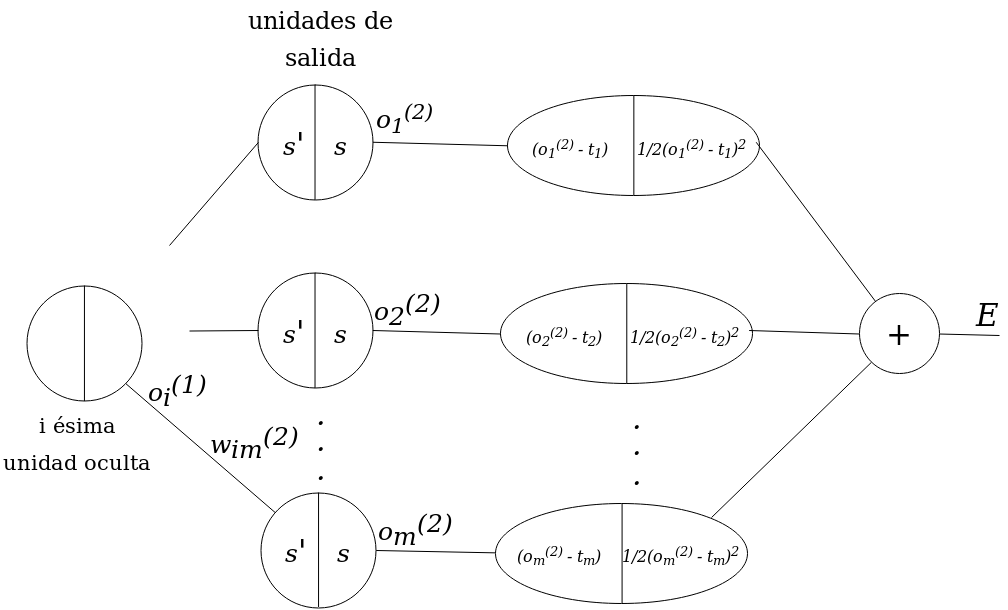
\includegraphics[scale=0.3]{extended_multilayer_network.png}
%     \caption{Red con múltiples capas extendida para el cáculo de $E$.}
%     \label{fig:extended_multilayer_net}
% \end{figure}

% Después de elegir los pesos de la red aleatoriamente, el algoritmo de propagación hacia atrás
% es usado para hacer las correcciones necesarias. El algoritmo puede descomponerse en los siguientes cuatro pasos:

% \begin{enumerate}
%     \item Cálculo feedforward
%     \item Retropropagación a la capa de salida
%     \item Retropropagación de la capa oculta
%     \item Actualización de pesos
% \end{enumerate}

% El algoritmo se detiene cuando el valor de la función de costo se ha vuelto lo suficientemente
% pequeño.

% \textbf{Primer paso: cálculo feedforward}. 

% \textbf{Segundo paso: retropropagación a la capa de salida}. Buscamos el primer
% conjunto de derivadas parciales $\frac{\partial E}{\partial w_{ij}^{(2)}}$. El camino de la 
% propagación hacia atrás desde la salida de la red hasta la unidad de salida $j$ se muestra
% en el diagrama B de la Figura \ref{fig:backprop_output}.

% \begin{figure}
%     \centering
%     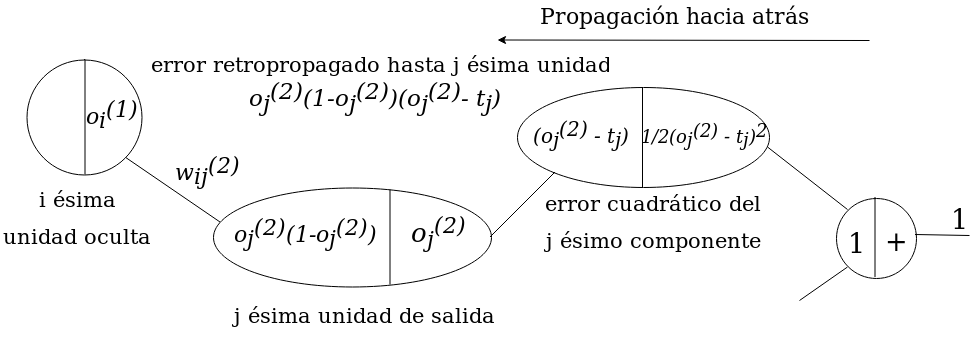
\includegraphics[scale=0.25]{backprop_hidden.png}
%     \caption{Camino de retropropagación hasta la unidad de salida $j$.}
%     \label{fig:backprop_output}
% \end{figure}

% Desde este camino se pueden recoger todos los términos multiplicativos que definen al
% error de retropropagación $\delta_j^{(2)}$. Por lo tanto

% \[
% \delta_j^{(2)}  = o_j^{(2)} (1-o_j^{(2)})(o_j^{(2)}-t_j)
% \]

% y la derivada parcial que buscamos es

% \[
% \frac{\partial E}{\partial w_{ij}^{(2)}} = [o_j^{(2)}(1-o_j^{(2)})(o_j^{(2)})(o_j^{(2)}-t_j)]o_j^{(1)} = \delta_j^{(2)}o_i^{(1)}
% \]

% Recordemos que para este último paso consideramos el peso $w_{ij}^{(2)}$ como una variables y su
% entrada $o_i^{(1)}$ una constante.

% En la Figura \ref{fig:backprop_edge_multi_net} se muestra la situación general que encontramos durante el algoritmo
% de propagación hacia atrás. En el lado de la entrada de arista con peso $w_{ij}$
% tenemos $o_i^{(1)}$ y en el lado de la salida el error retropropagado $\delta_j^{(2)}$.

% \begin{figure}
%     \centering
%     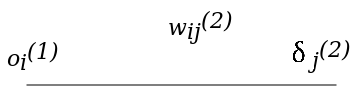
\includegraphics[scale=0.3]{backprop_edge.png}
%     \caption{Entrada y error retropropagado en una arista.}
%     \label{fig:backprop_edge_multi_net}
% \end{figure}

% \textbf{Tercer paso: retropropagación a la capa oculta}. Ahora queremos calcular las
% derivadas parciales $\frac{\partial E}{\partial w_{ij}^{(1)}}$. Cada unidad $j$ en la capa oculta
% está conectada a cada unidad $q$ en la capa de saida con una arista con pesos $w_{jq}^2$,
% para $q = 1, \dots, m$. El error retropropagado hasta la unidad $j$ en la capa oculta
% debe ser calculado tomando en cuenta todos los hacia atrás posibles, como se muestra en
% la Figura \ref{fig:backprop_multi_net_input}. El error retropropagado es entonces

% \[
% \delta_j^{(1)} = o_j^{(1)} (1-o_j^{(1)}) \sum_{q=1}^m w_{jq}^{(2)}\delta_q^{(2)}
% \]

% Por lo tanto la derivada parcial que estamos buscando es

% \[
% \frac{\partial E}{\partial w_{ij}^{(1)}} = \delta_j^{(1)}o_i
% \]

% El error retropropagado puede ser calculado de la misma manera para
% cualquier número de capas ocultas y la expresión para las derivadas
% parciales de $E$ se mantiene la misma forma analítica.

% \begin{figure}
%     \centering
%     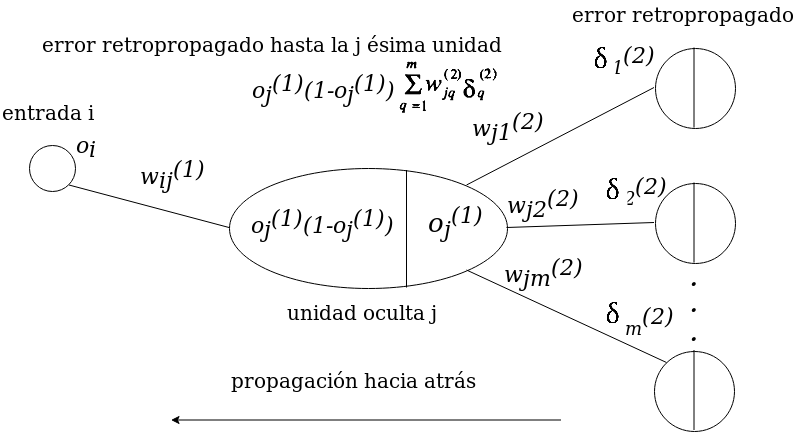
\includegraphics[scale=0.3]{backprop_input.png}
%     \caption{Todos los caminos hasta la entrada $i$.}
%     \label{fig:backprop_multi_net_input}
% \end{figure}


% \textbf{Cuarto paso: actualización de los pesos}. Después de calcular todas las derivadas
% parciales, los pesos de la red se actualizan en la dirección negativa del gradiente. Una
% constante de aprendizaje $\gamma$ define el tamaño del paso de la corrección. Las 
% correcciones para los pesos están dadas por

% \[
% \Delta w_{ij}^{(2)} = - \gamma o_i^{(1)}\delta_j^{(2)}, \mbox{ para }  i = 1, \dots, k+1; j = 1, \dots, m
% \]
% y

% \[
% \Delta w_{ij}^{(1)} = - \gamma o_i\delta_j^{(1)}, \mbox{ para }  i = 1, \dots, n+1; j = 1, \dots, k
% \]

% sabiendo que $o_{n+1} = o_{k+1}^{(1)} = 1$. Es muy importante hacer las
% correcciones de los pesos solamente después de haber calculado el error de retropropagación
% para todas las unidades en la red. De otro modo las correcciones se entrelazan con
% el error retropropagado y las correcciones calculadas ya no corresponden a la dirección del
% gradiente negativo. 

% \textbf{Más de una muestra de entrenamiento}. En el caso de $p > 1$ patrones de 
% entrada y salida, una red extendida se usa para calcular la función de costo
% para cada uno de ellos de manera separada. Las correcciones de los pesos se calculan
% para cada patrón y así obtenemos, por ejemplo, para el peso $w_{ij}^{(1)}$ las correcciones

% \[
% \Delta_1w_{ij}^{(1)}, \Delta_pw_{ij}^{(1)}, \dots, \Delta_pw_{ij}^{(1)}
% \]

% La actualizacion necesaria en la dirección del gradiente es entonces

% \[
% \Delta w_{ij}^{(1)} = \Delta_1w_{ij}^{(1)} + \Delta_2w_{ij}^{(1)} + \dots + \Delta_pw_{ij}^{(1)}
% \]

% Hablamos de actualizaciones \textit{offline} o por \textit{lotes} cuando la corrección
% de los pesos se hace de esta manera. Sin embargo, las actualizaciones de los pesos pueden hacerse
% secuencialmente después de presentar cada patrón, a esto se le llama entrenamiento \textit{online}.
% En este caso las correcciones no siguen exactamente la dirección del gradiente negativo,
% pero si los patrones de entrenamiento son seleccionados aleatoriamente la dirección de búsqueda
% oscila alrededor del la dirección exacta del gradiente y en la mayoría de los casos, el algoritmo
% implementa una forma de descenso en la función de costo. La razón de usar el entrenamiento
% online es que añade algo de ruido a la dirección del gradiente, lo que ayuda a evitar caer
% en mínimos locales de la función de costo. Además, cuando el conjunto de entrenamiento
% consiste en miles de patrones de entrenamiento, es muy costoso calcular la dirección 
% exacta del gradiente ya que cada \textit{época} (una ronda de presentación de todos
% los patrones de la red) consiste de muchos pasadas feedforward y el entrenamiento en
% línea se vuelve más eficiente.



% Hemos mostrado que en una red con una capa oculta y una de salida ($n, k$ y $m$ unidades)
% la entrada $\mathbf{o}$ produce la salida $\mathbf{o}^{(2)} = s(\mathbf{\hat{o}}^{(1)} \mathbf{W}_2)$
% donde $\mathbf{o}^{(1)} = s(\mathbf{\hat{o}}\mathbf{W}_1)$. En el paso de propagación hacia atrás sólo
% necesitamos las primeras $n$ filas de la matriz $\mathbf{W}_1$. Llamamos a esta matriz de $n \times k$, 
% $\mathbf{\overline{W}}_1$. Similarmente, a la matriz de $k \times m$ $\mathbf{\overline{W}}_2$
% compuesta por las primeras $k$ filas de la matriz $\mathbf{W}_2$. Asumimos esto porque no necesitamos 
% propagar hacia atrás valores  hacia las entradas constantes que corresponden a cada
% sesgo.

% Las derivadas almacenadas en el paso de feedforward en las $k$ unidades ocultas y
% las $m$ unidades de salida pueden ser escritas como las siguientes dos matrices diagonales. 
% Suponemos que nuestra función de activación en todas las unidades es la sigmoide.


% Definimos al vector $\mathbf{e}$ con las derivadas de las desviaciones cuadráticas como

% \[
% \mathbf{e} = 
% \begin{pmatrix}
%     (o_1^{(2)} - t_1) \\
%     (o_2^{(2)} - t_2) \\
%     \vdots \\
%     (o_m^{(2)} - t_m)
% \end{pmatrix}
% \]

% El vector $m$ dimensional $\boldsymbol{\delta^{(2)}}$ del error retropropagado hasta las 
% unidades de salida está dado por la expresión

% \[
% \boldsymbol{\delta}^{(2)} = \mathbf{D}_2\mathbf{e}
% \]


\subsection{Aprendizaje profundo}
El \textit{aprendizaje profundo} permite a las computadoras construir conceptos complejos
a partir de conceptos más simples. La Figura 
\ref{fig:deeplearning_person} muestra cómo un sistema de aprendizaje profundo
puede representar el concepto de la imagen de una persona al combinar conceptos más simples, tales
como esquinas y contornos, que a su vez están definidos en términos de los bordes.
El ejemplo por excelencia de un modelo de aprendizaje profundo es una \textit{red neuronal feedforward
profunda}, donde que sea profunda significa que tiene dos o más capas ocultas. Una red neuronal
es simplemente una función matemática que mapea algún conjunto de valores de entrada en 
valores de salida. La función está formada por una composición de funciones más simples.
Podemos suponer que al aplicar cada función matemática se obtiene una nueva representación de la
entrada.\\

\begin{remark}

El aprendizaje profundo es un tipo de aprendizaje automático
poderoso y flexible que aprende una representación del mundo
como una jerarquía anidada de conceptos, donde 
cada concepto está definido a partir de conceptos más simples,
y representaciones más abstractas calculadas en términos
de menos abstractas \cite{iangoodfellowyoshuabengioaaroncourville2017}.

\end{remark}


\begin{figure}
    \centering
    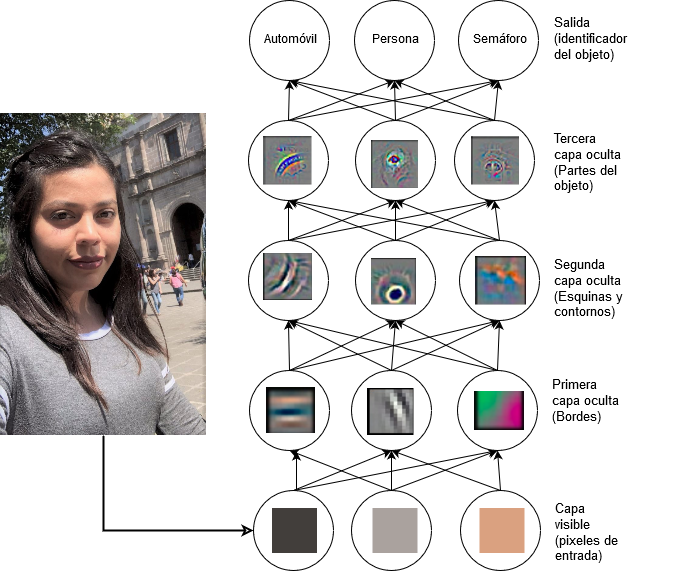
\includegraphics[scale=0.5]{figures/deep_learning_person.png}
    \caption{Ejemplo de un modelo de aprendizaje profundo. El aprendizaje profundo resuelve el problema de mapear un conjunto de pixeles al identificador de un objeto separando este mapeo
    complejo en mapeos simples anidados, cada uno descrito por
    una capa diferente en el modelo. La entrada es presentada
    en la capa visible, llamada así porque contiene las variables que somos capaces de observar. Después una serie de capas ocultas extraen de la imagen características cada vez más
    abstractas. Estas capas se llaman \textit{ocultas} porque
    sus valores no son dados en los datos; en su lugar, el modelo
    debe determinar qué conceptos son útiles para explicar 
    las relaciones de los datos observados. Dados los pixeles,
    la primera capa puede fácilmente identificar bordes comparando
    el brillo entre vecindades de pixeles.
    Dada la descripción de bordes de la primera capa, la segunda
    capa puede con facilidad buscar esquinas y contornos
    que son reconocibles como colecciones de bordes. Dada el 
    resultado de la segunda capa oculta, la tercera capa detecta
    partes enteras de objetos específicos, al encontrar
    colecciones específicas de contornos y esquinas. 
    Finalmente, esta descripción de la imagen en términos 
    de partes de objetos puede ser usada para reconoces objetos
    presentes en la imagen.\label{fig:deeplearning_person}}
    
\end{figure}
% La idea del aprender la representación correcta de los datos provee una perspectiva del aprendizaje
% profundo. Otra perspectiva sobre el aprendizaje profundo es que la profundidad permite a la
% computadora aprender un programa de varias etapas. Cada capa de la representación puede
% ser el estado de la memoria de la computadora después de ejecutar un conjunto de instrucciones
% en paralelo. Las redes con una profundidad mayor puede correr más instrucciones en secuencia. Las
% instrucciones en secuencia son poderosas porque instrucciones posteriores pueden hacer referencia
% a resultados de instrucciones previas. De acuerdo a este enfoque del aprendizaje profundo, no toda
% la información en las activaciones de una capa necesariamente codifica los factores de variación que
% explican la entrada. La representación también almacena información de estados que ayudan a la
% ejecución de un programa que puede dar sentido a la entrada. Esta información de estado puede ser
% análogo a un contador o a un apuntador en un programa de computadora tradicional. No tiene
% nada que ver con el contenido de la entrada específicamente, pero permite que el modelo
% se organice para su procesamiento.

% Hay dos maneras de medir la profundidad de un modelo. La primera es basándose en el número de 
% instrucciones secuenciales que deben ejecutarse para evaluar la arquitectura. 


\subsection{Redes neuronales convolucionales}

\begin{remark}
Las redes neuronales convolucionales o CNN (por sus siglas en inglés), son un tipo especializado
de red neuronal para procesamiento de datos que tienen una topología parecida a una cuadrícula. El nombre de 
red convolucional indica que la red ocupa una operación matemática llamada convolución. \cite{iangoodfellowyoshuabengioaaroncourville2017}.
\end{remark}


Las redes convolucionales son una categoría dentro de las redes neuronales profundas, que han 
demostrado ser muy efectivas en áreas como el reconocimiento y clasificación de imágenes. Debido
a los excelentes resultados de las CNN en estas áreas, nos enfocaremos en estas redes para tareas
de visión computacional.\\

% \subsubsection{La operación de convolución}
% Consideremos un filtro de dos dimensiones (también llamado máscara o kernel),
% $w(x, y)$, de tamaño $m \times n$. La correlación del filtro con una imagen $f(x,y)$,
% denotada como $w(x,y) \star f(x,y)$, está dada por:

% \begin{equation}\label{correlation}
%     w(x,y) \star f(x,y) = \sum_{s=-a}^a \sum_{t=-b}^b w(s,t)f(x+s, y+t)
% \end{equation}
% . Convolucionar el filtro con una imagen $I(n_1, n_2)$
% y producir la imagen $Z(n_1, n_2)$ se representa como sigue:

% \begin{equation*}
%     Z(n_1, n_2) = \sum_{l=0}^a\sum_{w=0}^b F(l, w) I(n_1+l, n_2+w) \forall n_1, n_2
% \end{equation*}

\begin{remark}
La correlación es una operación que funciona recorriendo una imagen y aplicando un
\textit{filtro} a cada pixel. El filtro se denota como un \textit{kernel}. Primero 
el kernel se llena con números llamados coeficientes de kernel. Estos coeficientes 
ponderan el valor del pixel que cubren y la salida de la correlación es la suma
de los valores de los pixeles ponderados. Matemáticamente la correlación de la imagen
$I$ con el kernel $K$ se puede expresar como
\begin{equation}\label{correlation}
    S(i,j) = (I * K)(i,j) = \sum_{m} \sum_{n} I(i+m, j+n) K(m,n).
\end{equation}
\end{remark}

% donde $m$ y $n$ son el largo y ancho del kernel respectivamente.
La correlación está asociada con el término de \textit{convolución} y ambos se utilizan
en el contexto de procesamiento de imágenes. La convolución únicamente difiere en la manera
en que el kernel se aplica a la imagen. Formalmente la convolución se define como

\[
S(i,j) = \sum_{m} \sum_{n} I(i-m, j-n) K(m,n).
\]

Comparando esta ecuación con la de correlación (ecuación \ref{correlation}), podemos
ver que las únicas diferencias son los signos negativos. La interpretación de esto
es que el kernel está rotado $180$ grados antes de hacer la correlación.

Cuando se aplica un filtro para suavizar una imagen, encontrar bordes, etcétera, el 
proceso se denota como convolución incluso si se implementa como una correlación. Por
lo tanto, por conveniencia llamaremos a ambas operaciones convolución.

\begin{figure}[htbp]
    \centering
    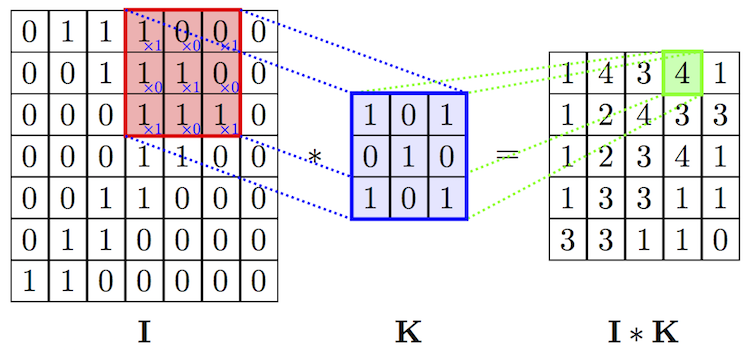
\includegraphics[scale=0.5]{conv_operation.png}
    \caption{Convolución entre una imagen
    $I$ y un kernel $K$ sin rotarlo 180 grados. Para este ejemplo $h = w = 7$ y $f = 3$.}
    \label{fig:convolution_example}
\end{figure}

En la Figura \ref{fig:convolution_example} para calcular
cada valor en la salida, el kernel se mueve con un paso 
de tamaño uno sobre el eje horizontal y vertical. Este paso
se conoce como \textit{zancada} o \textit{stride} (en inglés).
El valor de la zancada puede ser diferente de uno, según 
convenga. El tamaño de $I * K$ para una imagen $I$ de tamaño
$h \times w$ y un filtro de tamaño $f \times f$ depende también de
la zancada $s$.

\[
h' = \lfloor\frac{h-f+s}{s}\rfloor
\]

\[
w' = \lfloor\frac{w-f+s}{s}\rfloor
\]

donde $h'$ y $w'$ son las dimensiones del resultado.
Se puede notar que entre más grande sea el valor de $s$
el tamaño de $I * K$ disminuye. Sin embargo, en algunas 
aplicaciones es necesario conservar el tamaño de la entrada.
Esto último se logra aplicando un \textit{borde de ceros}
a la imagen de entrada. Al añadir el borde de ceros las
dimensiones el tamaño del resultado de la convolución se 
incrementa. Si $p$ denota el incremento sobre cada dimensión
de $I$, el tamaño de $h'$ y $w'$ se calculan de la siguiente 
forma:


\[
h' = \lfloor\frac{h-f+s+p}{s}\rfloor
\]

\[
w' = \lfloor\frac{w-f+s+p}{s}\rfloor
\]

% \subsubsection{Motivación}

La convolución aprovecha dos ideas importantes que pueden ayudar a mejorar un
sistema de aprendizaje automático: \textit{interacciones escasas} y \textit{compartición de parámetros}.

Las capas de las redes neuronales tradicionales usan la multiplicación de matrices de parámetros con
un parámetro separado entre cada unidad de entrada y cada unidad de salida. Esto significa que cada 
unidad de salida interactúa con cada unidad de entrada. Las redes convolucionales, sin embargo, 
tienen \textit{interacción escasa} (también conocida como 
conectividad escasa o pesos escasos). Esto se logra haciendo que el kernel sea de menor
tamaño que la entrada. Por ejemplo, cuando se procesa una imagen, la imagen de entrada puede tener 
miles o millones de pixeles, pero podemos detectar pequeñas y significativas características como
bordes con kernels que sólo ocupan decenas o cientos de pixeles. En consecuencia se puede ver
que se almacenan menos parámetros, lo que reduce los requisitos de memoria del modelo 
y mejora la eficiencia estadística. Además significa que el cálculo de las salidas requiere menos 
operaciones.

La \textit{compartición de parámetros} se refiere a usar el mismo parámetro para más de una función
en un modelo. En una red neuronal tradicional, cada elemento de la matriz de pesos se usa 
exactamente una vez cuando se calcula la salida de una capa. Se multiplican por un elemento en la 
entrada y nunca se vuelve a visitar. En una CNN, cada elemento del kernel se usa en cada posición de la
entrada. La compartición de parámetros indica que más que aprender un conjunto de parámetros 
por separado para cada posición, aprendemos sólo un conjunto. 


Sabemos que cada kernel puede verse como una cuadrícula de números también llamados pesos
y que éstos se aprenden durante el entrenamiento de la CNN. El proceso de aprendizaje involucra 
la inicialización de los pesos del kernel al comenzar el entrenamiento. Posteriormente, dados los pares
de entrada-salida, los pesos son ajustados en varias iteraciones durante el proceso de aprendizaje.\\

\begin{remark}
Un capa típica en una CNN consiste de tres etapas. En la 
primera etapa, la capa realiza diferentes convoluciones en
paralelo para producir una colección de mapas de
características. En la segunda etapa cada mapa 
de características se pasa por una función de activación
no lineal. La función de activación más común es el 
rectificador o ReLU definido como $g(z) = max(0, z)$.
Esta etapa también se conoce como detector.
En la tercera etapa utilizamos una función de agrupación
o pooling para modificar la salida de la capa aún más \cite{iangoodfellowyoshuabengioaaroncourville2017}.\\
\end{remark}

\begin{remark}
Una función de pooling reemplaza la salida de la red en cierta
ubicación con una estadística resumida de las salidas vecinas.
Por ejemplo, la operación de agrupamiento máximo
retorna el valor máximo dentro de una vecindad rectangular.
\end{remark}


El agrupamiento ayuda a hacer que la representación se vuelva 
aproximadamente invariante a pequeñas traslaciones de
la entrada. La \textit{invarianza a las traslaciones} significa 
que si trasladamos la entrada por una pequeña cantidad, los
valores de la mayoría de las salidas agrupadas no cambian.
La invarianza a traslaciones locales puede ser muy útil cuando
nos importa si una característica está presente y no 
exactamente dónde.

A las capas que pasan por las tres etapas las llamaremos \textit{capas
de convolución}, aunque para algunos autores, cada etapa es una capa
diferente, la primera es de convolución, la segunda de pooling y la 
tercera de no linealidad. Por simplicidad elegimos el término
de capa de convolución.

% La capa de convolución es el componente más importante de una CNN. Esta capa realiza la 
% convolución entre un conjunto de kernels y la entrada de la capa para producir como salida
% un colección de \textit{mapas de características}, donde cada uno de éstos es el resultado
% de la convolución entre un kernel y la entrada.


% \subsubsection{Pooling}

% \subsubsection{ReLU}
% En redes neuronales modernas, la función de activación estándar recomendada (principalmente
% para tareas de visión)
% es la \textit{unidad lineal rectificada} o ReLU (por sus siglas en inglés).
% Esta función mapea la entrada a $0$ si es negativa y mantiene el valor original
% si es positiva. Esto se representa como sigue

% \[
% f (x) = \max(0,x)
% \]

% \subsubsection{Entropía cruzada}

% La función de costo para una red convolucional se elige dependiendo
% de la tarea que se desea realizar. Por ejemplo, hasta ahora hemos utilizado
% la suma de errores cuadráticos; esta función se utiliza en tareas de
% regresión. Para tareas de clasificación en múltiples clases usamos como función de
% costo la \textit{entropía cruzada} definida como

% \[
% E_{log} = -\sum_p \sum_i t_{pi} \log(y_{pi})
% \]

% donde $y_{pi}$ es la probabilidad estimada de que el patrón $p$ que pertenezca
% a la clase $i$ y $t_{pi} \in \{0,1\}$ es el objetivo.

% La probabilidad de cada clase para un patrón $p$ puede ser calculada usando la función
% \textit{softmax}:

% \[
% y_{i} = \frac{e^{\hat{y}_i}}{\sum_k e^{\hat{y}_k}}
% \]

% donde $\hat{y}_i$ es la salida de la red de la unidad $i$ y la suma es sobre las 
% $k$ unidades de salida.

% \subsubsection{Dropout}

% Un problema central en el aprendizaje automático es cómo hacer que un algoritmo
% se desempeñe bien no sólo en el conjunto de entrenamiento, sino también con
% nuevos patrones de entrada. Muchas estrategias usadas en el aprendizaje automático están 
% diseñadas para reducir el error de prueba. Estas estrategias se conocen colectivamente 
% como \textit{regularización}.

% Definimos la regularización como cualquier modificación que hacemos a nuestro algoritmo de 
% aprendizaje con la intención de reducir el error de generalización pero no 
% el error de entrenamiento.

% Una de las estrategias más populares para la regularización de redes neuronales es
% el \textit{dropout}. Específicamente el dropout entrena el conjunto de todas las subredes que pueden
% ser formadas al remover las unidades que no son de salida a partir de una red base.
% % Consideremos una red neuronal completamente conectada compuesta por $L$ capas e indexadas por
% % $l $
% Para entrenar con dropout utilizamos un algoritmo de aprendizaje
% basado en lotes. Cada vez que tomamos una muestra del lote, aleatoriamente 
% muestreamos una máscara binaria que se aplica a todas las unidades ocultas y de
% entrada en la red. La máscta para cada unidad se muestrea independientemente de todas las
% demás. La probabilida de tomar una máscara con calor uno (causando que la unidad se incluya)




% \subsubsection{Convolución}
% \subsubsection{Pool}

% \subsubsection{ReLU}
% \subsubsection{Softmax}

% \subsection{Otros conceptos}
% \subsubsection{Entropía cruzada}
% \subsubsection{Dropout}
% \subsubsection{One-hot encoding}

\subsection{TensorFlow}

TensorFlow es una biblioteca de código abierto para computo numérico. Fue desarrollada 
originalmente por investigadores e ingenieros del equipo de Google Brain, con 
el propósito de motivar la investigación de arquitecturas profundas.

TensorFlow es una interfaz para expresar algoritmos de aprendizaje automático
y una implementación para ejecutar tales algoritmos.
Un cálculo expresado en TensorFlow puede ser ejecutado con ningún o con mínimos
cambios en una amplia variedad de sistemas desde dispositivos móviles
como teléfonos o tabletas hasta sistemas distribuidos a gran escala
de cientos de máquinas y cientos de dispositivos con unidades de procesamiento 
gráfico (GPU). El sistema es flexible y puede usarse para expresar una gran 
variedad de algoritmos, incluyendo algoritmos de entrenamiento
e inferencia para modelos de redes neuronales profundas y ha sido usado
para llevar a cabo investigaciones en áreas como la visión computacional,
robótica, procesamiento de lenguaje natural, etcétera.\\ 

\begin{remark}
Los cálculos en TensorFlow son descritos por una gráfica dirigida
que está compuesta por un conjunto de nodos y aristas.
La gráfica representa un cálculo de flujo de datos \cite{tensorflow} (un modelo
de programación para cómputo paralelo).
\end{remark}
A menudo los clientes construyen la gráfica de cómputo usando uno de los
lenguajes de frontend soportados (C++ o Python). Todos los ejemplos
que se muestran en esta sección están desarrollados en Python.

En una gráfica de TensorFlow los nodos representan instancias de \textit{operaciones}, éstos tienen cero o más entradas y
cero o más salidas. Los valores que fluyen sobre las aristas en la gráfica son
\textit{tensores}. Estos últimos son arreglos de dimensiones arbitrarias donde el tipo
de sus elementos se especifica o infiere durante la construcción de la gráfica.

Una \textit{operación} tiene un nombre y representa un cálculo abstracto, por ejemplo,
una multiplicación de matrices o una suma. 

Los programas clientes interactúan con el sistema de TensorFlow creando una
\textit{Session}. El objeto Session es una interfaz para la gráfica de cómputo,
es quien permite su ejecución a través de su operación primaria
\textit{Run}, la cual toma un conjunto de nodos de la gráfica que necesitan ser
calculados, así como un conjunto de tensores que necesitan alimentar a la 
gráfica para poder obtener las salidas de ciertos nodos. TensorFlow puede calcular
la cerradura transitiva de todos los nodos que deben ser ejecutados
para poder calcular las salidas que fueron solicitadas en los argumentos de \textit{Run}.

\begin{quote}
\begin{savenotes}\sphinxattablestart
\centering
\sphinxcapstartof{table}
\caption{Algunos de los tipos de operaciones en TensorFlow.}\label{\detokenize{chapter_one/tensorflow:operations}}
\sphinxaftercaption
%\begin{tabulary}

%%%%%%%%%%%%%%%5
\begin{tabulary}{\linewidth}[t]{|T|T|}
%\begin{tabulary}[t]{|c|c|}
\hline 
Categoría & Ejemplo \\ 
\hline 
Operaciones matemáticas a nivel de elementos & \texttt{Add, Sub, Mul, Div, Exp, Log, Greater, Less, Equal, ...} \\ 
\hline 
Operaciones con arreglos & \texttt{Concat, Slice, Split, Constant, Rank, Shape, Shuffle, ...} \\ 
\hline 
Operaciones con matrices & \texttt{MatMul, MatrixInverse, MatrixDeterminant, ...} \\ 
\hline 
Construcción de redes neuronales & \texttt{SoftMax, Sigmoid, ReLU, Convolution2D, MaxPool, ...} \\ 
\hline 
Operaciones de puntos de control & \texttt{Save, Restore, ...} \\ 
\hline 
\end{tabulary} 

%%%%%%%%%%%%%%%%5
% \end{tabulary}
\par
\sphinxattableend\end{savenotes}
\end{quote}
\subsubsection{Variables}

Cuando construimos un modelo de aprendizaje en TensorFlow utilizamos \textit{variables}
para representar los parámetros del modelo. Las variables de TensorFlow
son buffers en memoria que contienen tensores; pero a diferencia de los tensores
normales que sólo son instanciados cuando una gráfica se ejecuta y que 
inmediatamente después se eliminan, las variables se mantienen durante
múltiples ejecuciones de una gráfica. Como resultado, las variables de TensorFlow 
tienen las siguientes tres propiedades:

\begin{itemize}
\item Las variables deben inicializarse explícitamente antes de que una gráfica
se utilice por primera vez.
\item Podemos utilizar métodos de optimización como el del descenso del gradiente 
para modificar las variables después de cada iteración para ajustar los 
parámetros óptimos del modelo.
\item Podemos guardar en el disco los valores de las variables y restaurarlos
para su uso posterior.

\end{itemize}

Crear e inicializar una variable es muy simple,
únicamente utilizamos la clase \sphinxcode{Variable}
dentro de la biblioteca de TensorFlow.
Comencemos por inicializar una variable
que describe los pesos entre dos capas en una red neuronal.

\begin{sphinxVerbatim}[commandchars=\\\{\}]
\PYG{n}{weights} \PYG{o}{=} \PYG{n}{tf}\PYG{o}{.}\PYG{n}{Variable}\PYG{p}{(}\PYG{n}{tf}\PYG{o}{.}\PYG{n}{random\PYGZus{}normal}\PYG{p}{(}\PYG{p}{[}\PYG{l+m+mi}{300}\PYG{p}{,} \PYG{l+m+mi}{200}\PYG{p}{]}\PYG{p}{,} \PYG{n}{stddev}\PYG{o}{=}\PYG{l+m+mf}{0.5}\PYG{p}{)}\PYG{p}{,}
\PYG{n}{name}\PYG{o}{=}\PYG{l+s+s2}{\PYGZdq{}}\PYG{l+s+s2}{weights}\PYG{l+s+s2}{\PYGZdq{}}\PYG{p}{)}
\end{sphinxVerbatim}

\sphinxcode{tf} es un alias para el módulo \sphinxcode{tensorflow}.
\sphinxcode{tf.Variable} recibe dos argumentos; el primero,
\sphinxcode{tf.random\_normal}, que es una operación que
produce un tensor inicializado usando una
distribución normal con una desviación estándar de
0.5 y media 0. El tamaño del tensor es de $300 \times
200$, lo que significa que los pesos conectan a una
capa de 300 neuronas a una de 200. El segundo
parámetro es un identificador único que nos
permite referirnos a un nodo en específico en
la gráfica de cómputo.

Por defecto las variables son entrenables,
lo que quiere decir que cuando utilizamos un método
como el descenso del gradiente, las variables
automáticamente cambian sus valores.


\subsubsection{Placeholder}

Los modelos de aprendizaje necesitan una entrada ya sea 
para el entrenamiento o la evaluación. Una variable no es 
suficiente porque sólo se inicializa una vez. Necesitamos un
componente que llenemos cada que la gráfica de cómputo se ejecuta.
TensorFlow usa una estructura llamada \textit{placeholder}. 

Un placeholder es instanciado como sigue y puede ser utilizado en operaciones como los tensores
y variables en TensorFlow.

\begin{sphinxVerbatim}[commandchars=\\\{\}]
\PYG{n}{x} \PYG{o}{=} \PYG{n}{tf}\PYG{o}{.}\PYG{n}{Placeholder}\PYG{p}{(}\PYG{n}{tf}\PYG{o}{.}\PYG{n}{float32}\PYG{p}{,} \PYG{n}{name}\PYG{o}{=}\PYG{l+s+s2}{\PYGZdq{}}\PYG{l+s+s2}{x}\PYG{l+s+s2}{\PYGZdq{}}\PYG{p}{,} \PYG{n}{shape}\PYG{p}{[}\PYG{k+kc}{None}\PYG{p}{,} \PYG{l+m+mi}{1024}\PYG{p}{]}\PYG{p}{)}
\PYG{n}{W} \PYG{o}{=} \PYG{n}{tf}\PYG{o}{.}\PYG{n}{Variable}\PYG{p}{(}\PYG{n}{tf}\PYG{o}{.}\PYG{n}{random\PYGZus{}uniform}\PYG{p}{(}\PYG{p}{[}\PYG{l+m+mi}{784}\PYG{p}{,}\PYG{l+m+mi}{10}\PYG{p}{]}\PYG{p}{,} \PYG{o}{\PYGZhy{}}\PYG{l+m+mi}{1}\PYG{p}{,} \PYG{l+m+mi}{1}\PYG{p}{)}\PYG{p}{,} \PYG{n}{name}\PYG{o}{=}\PYG{l+s+s2}{\PYGZdq{}}\PYG{l+s+s2}{W}\PYG{l+s+s2}{\PYGZdq{}}\PYG{p}{)}
\PYG{n}{multiply} \PYG{o}{=} \PYG{n}{tf}\PYG{o}{.}\PYG{n}{matmul}\PYG{p}{(}\PYG{n}{x}\PYG{p}{,} \PYG{n}{W}\PYG{p}{)}
\end{sphinxVerbatim}

En el ejemplo definimos un placeholder donde \sphinxcode{x}
representa un lote de datos de tipo \sphinxcode{float32}.
Podemos notar que \sphinxcode{x} tiene 1024 columnas, lo
que significa que cada patrón de entrada
tiene una dimensión de 1024. Se puede notar también
que \sphinxcode{x} tiene un número indefinido de filas.
Esto significa que \sphinxcode{x} puede ser inicializado
con un número arbitrario de muestras. Aunque podemos
multiplicar cada muestra por separado con \sphinxcode{W},
al expresar un lote completo como un tensor tenemos
permitido calcular los resultados de todas los
patrones de entrada en paralelo. El
resultado de la fila $i$ del tensor de
multiplicación corresponde a multiplicar \sphinxcode{W}
con el patrón $i$.

Así como las variables se inicializan la primera vez
que se construye la gráfica, los placeholder necesitan
llenarse cada vez que se ejecuta la gráfica o una
subgráfica de cómputo.


\subsubsection{Ejemplo de una red neuronal en TensorFlow}

En este apartado se describe la creación de un modelo de aprendizaje muy
simple, una red neuronal, en TensorFlow para el cálculo de la función
\textbf{XOR}.


Como estamos en el contexto del aprendizaje automático
supervisado, necesitamos un conjunto de datos etiquetado.
Nuestro conjunto de datos está dado por la Tabla \ref{table:xor}. Las
primeras dos columnas son los atributos $X_1$ y $X_2$ y la tercera 
columna es el objetivo.


\begin{quote}
\begin{savenotes}\sphinxattablestart
\centering
\sphinxcapstartof{table}
\caption{Definición de la función XOR.\label{table:xor}}
\sphinxaftercaption
\begin{tabulary}{\linewidth}[t]{|c|c|c|}
\hline 
$X_1$ & $X_2$ & $Y = X_1 \oplus X2$ \\ 
\hline 
0 & 0 & 0 \\ 
\hline 
1 & 0 & 1 \\ 
\hline 
0 & 1 & 1 \\ 
\hline 
1 & 1 & 0 \\ 
\hline 
\end{tabulary} 
\par
\sphinxattableend\end{savenotes}
\end{quote}


La arquitectura de nuestra red es la siguiente: una capa de entrada con dos unidades
de entrada $X_1$ y $X_2$. Una capa oculta con dos unidades, que tienen como función
de activación la sigmoide. Por último una unidad de salida con la función sigmoide.
De manera gráfica esto se puede ver en la Figura \ref{image:xor_net}.

\begin{figure}[ht]
\centering
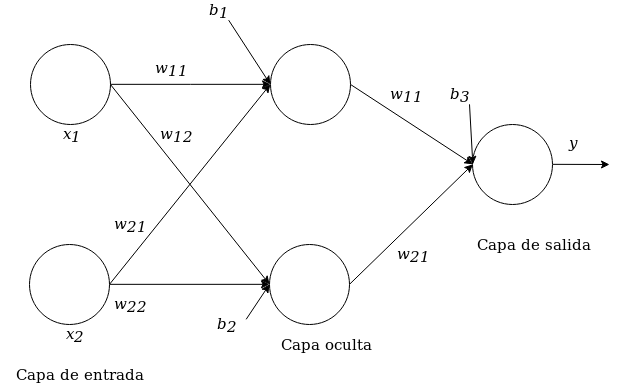
\includegraphics[scale=0.5]{xor_net.png}
\caption{\label{image:xor_net} Arquitectura de la red neuronal para calcular la función $\oplus$.}
\end{figure} 

Antes de comenzar con el código conviene dibujar la gráfica de cómputo que
deseamos ejecutar.
La gráfica de cómputo está descrita en la Figura \ref{fig:xor_graph}.
Los círculos representan o variables o placeholders excepto para
la salida predicha $y'$ que es el resultado de una operación. Tenemos
un placeholder para 
las entradas $X$ y otro para las salidas correctas u objetivos $y$. Las variables
son los pesos $W_i$ y los sesgos $b_i$.
Los rectángulos son las operaciones. En una red neuronal las únicas operaciones
son la multiplicación y suma de tensores, la aplicación de la función de
activación y un método de optimización como el descenso del gradiente para
minimizar el error dado por una función de costo, en nuestro caso
la suma de errores cuadráticos (SSE). 
Durante la ejecución de la gráfica las variables cambiarán su valor
automáticamente a los valores óptimos que minimicen el error.

\begin{figure}[ht]
\centering
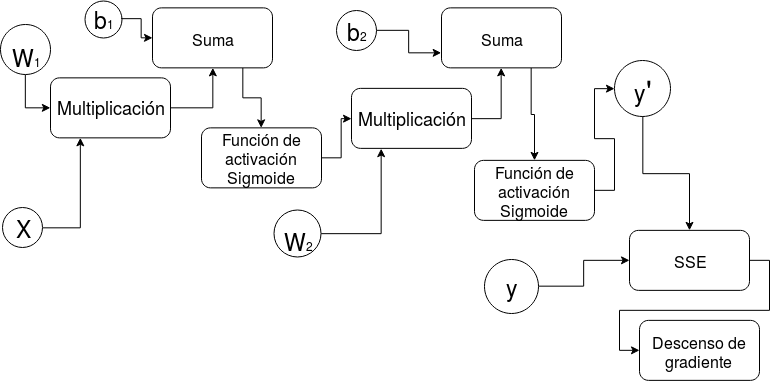
\includegraphics[scale=0.45]{xor_tf_graph.png}
\caption{\label{fig:xor_graph}La gráfica de TensorFlow que representa a la arquitectura de la red para
el cálculo de la función $\oplus$.}
\end{figure}


Un programa en TensorFlow se compone de dos partes,
la creación de la gráfica y su ejecución.

Antes que nada como para cualquier biblioteca, se importa \sphinxcode{tensorflow}.

\begin{sphinxVerbatim}[commandchars=\\\{\}]
\PYG{k+kn}{import} \PYG{n+nn}{tensorflow} \PYG{k}{as} \PYG{n+nn}{tf}
\end{sphinxVerbatim}

El conjunto de datos se puede definir en dos listas, una con los datos
de entrada y la otra con sus respectivas salidas.

\begin{sphinxVerbatim}[commandchars=\\\{\}]
\PYG{n}{datos\PYGZus{}de\PYGZus{}entrada} \PYG{o}{=} \PYG{p}{[}\PYG{p}{[}\PYG{l+m+mf}{0.}\PYG{p}{,} \PYG{l+m+mf}{0.}\PYG{p}{]}\PYG{p}{,} \PYG{p}{[}\PYG{l+m+mf}{1.}\PYG{p}{,} \PYG{l+m+mf}{0.}\PYG{p}{]}\PYG{p}{,} \PYG{p}{[}\PYG{l+m+mf}{0.}\PYG{p}{,} \PYG{l+m+mf}{1.}\PYG{p}{]}\PYG{p}{,} \PYG{p}{[}\PYG{l+m+mf}{1.}\PYG{p}{,} \PYG{l+m+mf}{1.}\PYG{p}{]}\PYG{p}{]} \PYG{c+c1}{\PYGZsh{} una lista con los diferentes pares (x1, x2)}
\PYG{n}{y} \PYG{o}{=} \PYG{p}{[}\PYG{p}{[}\PYG{l+m+mf}{0.}\PYG{p}{]}\PYG{p}{,} \PYG{p}{[}\PYG{l+m+mf}{1.}\PYG{p}{]}\PYG{p}{,} \PYG{p}{[}\PYG{l+m+mf}{1.}\PYG{p}{]}\PYG{p}{,} \PYG{p}{[}\PYG{l+m+mf}{0.}\PYG{p}{]}\PYG{p}{]} \PYG{c+c1}{\PYGZsh{}los objetivos o etiquetas}
\end{sphinxVerbatim}


\paragraph{Definición de la gráfica de cómputo}

Se definen los placeholders que se llenan con los patrones de entrada y sus etiquetas.

\begin{sphinxVerbatim}[commandchars=\\\{\}]
\PYG{n}{entrada\PYGZus{}de\PYGZus{}la\PYGZus{}red} \PYG{o}{=} \PYG{n}{tf}\PYG{o}{.}\PYG{n}{placeholder}\PYG{p}{(}\PYG{n}{tf}\PYG{o}{.}\PYG{n}{float32}\PYG{p}{,} \PYG{n}{shape}\PYG{o}{=}\PYG{p}{[}\PYG{l+m+mi}{4}\PYG{p}{,} \PYG{l+m+mi}{2}\PYG{p}{]}\PYG{p}{)} \PYG{c+c1}{\PYGZsh{} el placeholder que se llena con los datos\PYGZus{}de\PYGZus{}entrada}
\PYG{n}{salidas\PYGZus{}correctas} \PYG{o}{=} \PYG{n}{tf}\PYG{o}{.}\PYG{n}{placeholder}\PYG{p}{(}\PYG{n}{tf}\PYG{o}{.}\PYG{n}{float32}\PYG{p}{,} \PYG{n}{shape}\PYG{o}{=}\PYG{p}{[}\PYG{l+m+mi}{4}\PYG{p}{,} \PYG{l+m+mi}{1}\PYG{p}{]}\PYG{p}{)} \PYG{c+c1}{\PYGZsh{} placeholder para las etiquetas}
\end{sphinxVerbatim}

Después se crean las variables para los pesos y sesgos de la red, los parámetros que se aprenden.

\begin{sphinxVerbatim}[commandchars=\\\{\}]
\PYG{n}{weights\PYGZus{}layer\PYGZus{}one} \PYG{o}{=} \PYG{n}{tf}\PYG{o}{.}\PYG{n}{Variable}\PYG{p}{(}\PYG{n}{tf}\PYG{o}{.}\PYG{n}{random\PYGZus{}normal}\PYG{p}{(}\PYG{p}{[}\PYG{l+m+mi}{2}\PYG{p}{,} \PYG{l+m+mi}{2}\PYG{p}{]}\PYG{p}{)}\PYG{p}{)} \PYG{c+c1}{\PYGZsh{} valores aleatorios de la distribución normal media=0.0 desviación estándar=1.0}
\PYG{n}{weights\PYGZus{}layer\PYGZus{}two} \PYG{o}{=} \PYG{n}{tf}\PYG{o}{.}\PYG{n}{Variable}\PYG{p}{(}\PYG{n}{tf}\PYG{o}{.}\PYG{n}{random\PYGZus{}normal}\PYG{p}{(}\PYG{p}{[}\PYG{l+m+mi}{2}\PYG{p}{,} \PYG{l+m+mi}{1}\PYG{p}{]}\PYG{p}{)}\PYG{p}{)} \PYG{c+c1}{\PYGZsh{} media=0.0 desviación estándar=1.0}
\PYG{n}{bias\PYGZus{}layer\PYGZus{}one} \PYG{o}{=} \PYG{n}{tf}\PYG{o}{.}\PYG{n}{Variable}\PYG{p}{(}\PYG{n}{tf}\PYG{o}{.}\PYG{n}{random\PYGZus{}normal}\PYG{p}{(}\PYG{p}{[}\PYG{l+m+mi}{2}\PYG{p}{]}\PYG{p}{)}\PYG{p}{)} \PYG{c+c1}{\PYGZsh{} media=0.0 desviación estándar=1.0}
\PYG{n}{bias\PYGZus{}layer\PYGZus{}two} \PYG{o}{=} \PYG{n}{tf}\PYG{o}{.}\PYG{n}{Variable}\PYG{p}{(}\PYG{n}{tf}\PYG{o}{.}\PYG{n}{random\PYGZus{}normal}\PYG{p}{(}\PYG{p}{(}\PYG{p}{)}\PYG{p}{)}\PYG{p}{)} \PYG{c+c1}{\PYGZsh{} media=0.0 desviación estándar=1.0}
\end{sphinxVerbatim}

Necesitamos las operaciones que aplican la función de activación del resultado
de la suma del producto de los pesos con las entradas más los segos. Estas operaciones
generan la capa oculta. La salida de la red se compone de las mismas operaciones
pero sus entradas son las salidas de la capa oculta.

\begin{sphinxVerbatim}[commandchars=\\\{\}]
\PYG{n}{output\PYGZus{}layer\PYGZus{}one} \PYG{o}{=} \PYG{n}{tf}\PYG{o}{.}\PYG{n}{sigmoid}\PYG{p}{(}\PYG{n}{tf}\PYG{o}{.}\PYG{n}{matmul}\PYG{p}{(}\PYG{n}{entrada\PYGZus{}de\PYGZus{}la\PYGZus{}red}\PYG{p}{,} \PYG{n}{weights\PYGZus{}layer\PYGZus{}one}\PYG{p}{)} \PYG{o}{+} \PYG{n}{bias\PYGZus{}layer\PYGZus{}one}\PYG{p}{)}
\PYG{n}{network\PYGZus{}output} \PYG{o}{=} \PYG{n}{tf}\PYG{o}{.}\PYG{n}{sigmoid}\PYG{p}{(}\PYG{n}{tf}\PYG{o}{.}\PYG{n}{matmul}\PYG{p}{(}\PYG{n}{output\PYGZus{}layer\PYGZus{}one}\PYG{p}{,} \PYG{n}{weights\PYGZus{}layer\PYGZus{}two}\PYG{p}{)} \PYG{o}{+} \PYG{n}{bias\PYGZus{}layer\PYGZus{}two}\PYG{p}{)}
\end{sphinxVerbatim}

Se define la función de costo que se desea minimizar, la SSE.

\begin{sphinxVerbatim}[commandchars=\\\{\}]
\PYG{n}{error} \PYG{o}{=} \PYG{n}{tf}\PYG{o}{.}\PYG{n}{reduce\PYGZus{}sum}\PYG{p}{(}\PYG{n}{tf}\PYG{o}{.}\PYG{n}{square}\PYG{p}{(}\PYG{n}{salidas\PYGZus{}correctas} \PYG{o}{\PYGZhy{}} \PYG{n}{network\PYGZus{}output}\PYG{p}{)}\PYG{p}{)}
\end{sphinxVerbatim}

Elegimos el optimizador de la red para minimizar el error cambiando los parámetros (pesos y sesgos), ocupamos el descenso del gradiente (retropropagación).

\begin{sphinxVerbatim}[commandchars=\\\{\}]
\PYG{n}{optimizer} \PYG{o}{=} \PYG{n}{tf}\PYG{o}{.}\PYG{n}{train}\PYG{o}{.}\PYG{n}{GradientDescentOptimizer}\PYG{p}{(}\PYG{n}{learning\PYGZus{}rate}\PYG{o}{=}\PYG{l+m+mf}{0.1}\PYG{p}{)}
\PYG{n}{train} \PYG{o}{=} \PYG{n}{optimizer}\PYG{o}{.}\PYG{n}{minimize}\PYG{p}{(}\PYG{n}{error}\PYG{p}{)}
\end{sphinxVerbatim}

\paragraph{Ejecución de la gráfica de cómputo}

Finalmente se ejecuta la gráfica de TensorFlow. Se crea una instancia de \sphinxcode{Session} e iteramos ejecutando el método \sphinxcode{run}
que ejecuta el entrenamiento del modelo.



\begin{sphinxVerbatim}[commandchars=\\\{\}]
\PYG{k}{with} \PYG{n}{tf}\PYG{o}{.}\PYG{n}{Session}\PYG{p}{(}\PYG{p}{)} \PYG{k}{as} \PYG{n}{sess}\PYG{p}{:}
    \PYG{n}{sess}\PYG{o}{.}\PYG{n}{run}\PYG{p}{(}\PYG{n}{tf}\PYG{o}{.}\PYG{n}{global\PYGZus{}variables\PYGZus{}initializer}\PYG{p}{(}\PYG{p}{)}\PYG{p}{)} \PYG{c+c1}{\PYGZsh{}inicializa las Variables}
    \PYG{n}{epocas} \PYG{o}{=} \PYG{l+m+mi}{10000}
    \PYG{n+nb}{print}\PYG{p}{(}\PYG{l+s+s2}{\PYGZdq{}}\PYG{l+s+s2}{Salida de la red antes del entrenamiento:}\PYG{l+s+si}{\PYGZob{}\PYGZcb{}}\PYG{l+s+s2}{\PYGZdq{}}\PYG{o}{.}\PYG{n}{format}\PYG{p}{(}\PYG{n}{sess}\PYG{o}{.}\PYG{n}{run}\PYG{p}{(}\PYG{n}{network\PYGZus{}output}\PYG{p}{,} \PYG{n}{feed\PYGZus{}dict}\PYG{o}{=}\PYG{p}{\PYGZob{}}\PYG{n}{entrada\PYGZus{}de\PYGZus{}la\PYGZus{}red} \PYG{p}{:} \PYG{n}{datos\PYGZus{}de\PYGZus{}entrada}\PYG{p}{,} \PYG{n}{salidas\PYGZus{}correctas} \PYG{p}{:} \PYG{n}{y}\PYG{p}{\PYGZcb{}}\PYG{p}{)}\PYG{p}{)}\PYG{p}{)}
    \PYG{k}{for} \PYG{n}{i} \PYG{o+ow}{in} \PYG{n+nb}{range}\PYG{p}{(}\PYG{n}{epocas}\PYG{p}{)}\PYG{p}{:}
        \PYG{n}{sess}\PYG{o}{.}\PYG{n}{run}\PYG{p}{(}\PYG{n}{train}\PYG{p}{,} \PYG{n}{feed\PYGZus{}dict}\PYG{o}{=}\PYG{p}{\PYGZob{}}\PYG{n}{entrada\PYGZus{}de\PYGZus{}la\PYGZus{}red}\PYG{p}{:} \PYG{n}{datos\PYGZus{}de\PYGZus{}entrada}\PYG{p}{,} \PYG{n}{salidas\PYGZus{}correctas}\PYG{p}{:} \PYG{n}{y}\PYG{p}{\PYGZcb{}}\PYG{p}{)}
    \PYG{n+nb}{print}\PYG{p}{(}\PYG{l+s+s2}{\PYGZdq{}}\PYG{l+s+s2}{Salida de la red después del entrenamiento:}\PYG{l+s+si}{\PYGZob{}\PYGZcb{}}\PYG{l+s+s2}{\PYGZdq{}}\PYG{o}{.}\PYG{n}{format}\PYG{p}{(}\PYG{n}{sess}\PYG{o}{.}\PYG{n}{run}\PYG{p}{(}\PYG{n}{network\PYGZus{}output}\PYG{p}{,} \PYG{n}{feed\PYGZus{}dict}\PYG{o}{=}\PYG{p}{\PYGZob{}}\PYG{n}{entrada\PYGZus{}de\PYGZus{}la\PYGZus{}red} \PYG{p}{:} \PYG{n}{datos\PYGZus{}de\PYGZus{}entrada}\PYG{p}{,} \PYG{n}{salidas\PYGZus{}correctas} \PYG{p}{:} \PYG{n}{y}\PYG{p}{\PYGZcb{}}\PYG{p}{)}\PYG{p}{)}\PYG{p}{)}
\end{sphinxVerbatim}

La salida del programa es la siguiente:

\begin{sphinxVerbatim}[commandchars=\\\{\}]
Salida de la red antes del entrenamiento:
\PYG{o}{[}\PYG{o}{[}\PYG{l+m}{0}.3293548 \PYG{o}{]}
 \PYG{o}{[}\PYG{l+m}{0}.32501128\PYG{o}{]}
 \PYG{o}{[}\PYG{l+m}{0}.20175578\PYG{o}{]}
 \PYG{o}{[}\PYG{l+m}{0}.20124543\PYG{o}{]}\PYG{o}{]}
Salida de la red después del entrenamiento:
\PYG{o}{[}\PYG{o}{[}\PYG{l+m}{0}.03212966\PYG{o}{]}
 \PYG{o}{[}\PYG{l+m}{0}.9716061 \PYG{o}{]}
 \PYG{o}{[}\PYG{l+m}{0}.9716902 \PYG{o}{]}
 \PYG{o}{[}\PYG{l+m}{0}.02967284\PYG{o}{]}\PYG{o}{]}
\end{sphinxVerbatim}


% \section{Cómputo en la nube}
\label{\detokenize{chapter_one/cloud_computing:computo-en-la-nube}}\label{\detokenize{chapter_one/cloud_computing::doc}}

\begin{remark}
Según el Instituto Nacional de Estándares y Tecnología (NIST por sus siglas en inglés) de Estados Unidos;
el cómputo en la
nube se define como un modelo que hace posible el acceso ubicuo, conveniente
y bajo demanda a un grupo de recursos informáticos configurables
(p.ej. servidores, almacenamiento, redes, aplicaciones, y servicios) a través
de una red donde pueden ser rápidamente suministrados y
lanzados con un mínimo esfuerzo de mantenimiento
o interacción con los proveedores de servicios.
\end{remark}


El cómputo en la nube también se puede definir como un \textit{estilo de cómputo en el cual
se brindan recursos como servicios, bajo demanda, a través de internet}.
Estos recursos se escalan dinámicamente y a menudo son virtualizados.

Con esta tecnología los usuarios, casi con cualquier dispositivo, pueden acceder mediante internet
a programas, servicios de alojamiento de archivos, plataformas para desarrollo de
aplicaciones, etcétera; usando servicios ofrecidos por
proveedores de cómputo en la nube. Las ventajas del cómputo en la nube incluyen
reducción de costos, alta disponibilidad y la fácil escalabilidad.


\subsection{Capas del cómputo en la nube}
\label{\detokenize{chapter_one/cloud_computing:capas-del-computo-en-la-nube}}
El cómputo en la nube puede verse como una colección de servicios, que puede se
presentada como una arquitectura de cómputo en la nube en capas. Estas
tres capas son: \textit{Software as a Service (SaaS)},
\textit{Infrastructure as a Service (IaaS)} y \textit{Platform as a Service (PaaS)}.

\begin{figure}[ht]
\centering
\capstart

\noindent\sphinxincludegraphics[scale=0.75]{{cloud_computing_layers}.png}
\caption{Arquitectura en capas del cómputo en la nube}\label{\detokenize{chapter_one/cloud_computing:c-c-layers}}\end{figure}


\subsubsection{Software as a Service (SaaS)}
\label{\detokenize{chapter_one/cloud_computing:software-as-a-service-saas}}
El \sphinxstyleemphasis{Software como un Servicio} se refiere simplemente a software que se entrega
bajo demanda para su uso. Pongamos el siguiente ejemplo; antes si alguien necesitaba
un programa para edición de textos tenía que ir a una tienda, comprar algún disco, e instalarlo
en su computadora. Tiempo después una nueva actualización salía al mercado, entonces
se repetía el proceso.
Con SaaS, sólo es necesario ingresar desde el navegador a un programa
alojado en alguna parte. No hay instalación, no hay actualización.


\subsubsection{Infrastructure as a Service (IaaS)}
\label{\detokenize{chapter_one/cloud_computing:infrastructure-as-a-service-iaas}}
La \sphinxstyleemphasis{Infraestructura como un servicio} hace referencia a recursos de cómputo como un servicio.
Esto incluye computadoras
virtualizadas con garantía de poder de procesamiento y ancho de banda reservado para
almacenamiento y acceso a internet. Los servicios más comunes de la IaaS son:
\begin{itemize}
\item {} 
Alojamiento

\item {} 
Balance de carga

\item {} 
Conectividad de red púbica y privada

\item {} 
Firewalls

\item {} 
Almacenamiento

\end{itemize}


\subsubsection{Platform as a Service (PaaS)}
\label{\detokenize{chapter_one/cloud_computing:platform-as-a-service-paas}}
Esta se encuentra en medio de las otras dos,
con IaaS en la parte de abajo y SaaS en la parte más alta.
Se encarga de proveer todo lo necesario para ejecutar
un lenguaje en específico o un \sphinxstyleemphasis{stack de soluciones}. Es similar a IaaS pero incluye
un sistema operativo y servicios requeridos para una aplicación en específico.


\subsection{Servicios en la nube}
\label{\detokenize{chapter_one/cloud_computing:servicios-en-la-nube}}
Existen tres categorías de servicios en la nube. La primera es el servicio en la
nube SaaS, donde la aplicación entera corre en la nube. El cliente utiliza un
navegador para acceder a la aplicación. Un ejemplo de SaaS es Office 365.

El otro tipo de servicio es en el que la aplicación corre del lado del cliente,
sin embargo, accede a algunas funcionalidad y servicios provistos en el la nube.
Un ejemplo es Spotify. La aplicación móvil reproduce la música, mientras que el
servicio en la nube es utilizado para descargar nuevas canciones.

El último tipo es una plataforma en la nube para crear aplicaciones, usada por
desarrolladores. Los desarrolladores crean una nueva aplicación como SaaS  usando
una plataforma en la nube, un ejemplo es Cloud9.

\begin{figure}[ht]
\centering
\capstart

\noindent\sphinxincludegraphics[scale=0.75]{{cloud_services_categories}.png}
\caption{Las categorías de los servicios en la nube.}\label{\detokenize{chapter_one/cloud_computing:c-s-categories}}\end{figure}


\subsection{Tipos de cómputo en la nube}
\label{\detokenize{chapter_one/cloud_computing:tipos-de-computo-en-la-nube}}
Hay tres tipos de cómputo en la nube:
\begin{itemize}
\item {} 
\sphinxstylestrong{Nube pública}

\item {} 
\sphinxstylestrong{Nube privada}

\item {} 
\sphinxstylestrong{Nube híbrida}

\end{itemize}

En la nube pública, los recursos de cómputo son proporcionados dinámicamente a
través de internet por medio de aplicaciones web o servicios web brindados por
terceros. Las nubes públicas son ejecutadas por terceros y la aplicaciones de
diferentes consumidores probablemente se mezclan en los servidores en la nube,
los sistemas de almacenamiento y las redes.

La nube privada es el cómputo en la nube sobre redes privadas. Están construidas
exclusivamente para un cliente, proporcionando un control total sobre los datos,
la seguridad y la calidad del servicio. La nube privada puede ser mantenida por
la organización que la ocupará o por terceros.

Una nube híbrida combina múltiples modelos de nubes privadas y públicas. Añaden
la complejidad de determinar como distribuir aplicaciones entre ambos tipos de nubes.


\subsection{Cómputo en la nube vs servicios en la nube}
\label{\detokenize{chapter_one/cloud_computing:computo-en-la-nube-vs-servicios-en-la-nube}}
En esta sección se presentan dos tablas que muestran las diferencias y los principales
atributos del cómputo en la nube y los servicios en la nube. El cómputo en la nube
consiste de las tecnologías que permiten los servicios en la nube. Los atributos
clave del cómputo en la nube y de los servicios en la nube se muestran en las
tablas  \ref{\detokenize{chapter_one/cloud_computing:key-cloud-computing-attr}} y  \ref{\detokenize{chapter_one/cloud_computing:key-cloud-services-attr}}, respectivamente.


\begin{savenotes}\sphinxattablestart
\centering
\sphinxcapstartof{table}
\caption{Atributos principales del cómputo en la nube \label{\detokenize{chapter_one/cloud_computing:key-cloud-computing-attr}}}
\sphinxaftercaption
\begin{tabulary}{\linewidth}[t]{|T|T|}
\hline
\sphinxstylethead{ 
Atributo
\unskip}\relax &\sphinxstylethead{ 
Descripción
\unskip}\relax \\
\hline
Sistemas de infraestructura
&
Incluye servidores, almacenamiento, y redes que pueden escalarse como el usuario lo demande.
\\
\hline
Aplicación
&
Provee una interfaz de usuario basada en la web., servicios web de API, y una amplia variedad de configuraciones.
\\
\hline
Desarrollo aplicaciones y lanzamiento de software
&
Soporta el desarrollo e integración de una aplicación de software en la nube.
\\
\hline
Software de mantenimiento para sistemas y aplicaciones
&
Soporta una provisión rápida de autoservicio y configuración, además de un monitoreo de uso.
\\
\hline
\end{tabulary}
\par
\sphinxattableend\end{savenotes}


\begin{savenotes}\sphinxattablestart
\centering
\sphinxcapstartof{table}
\caption{Atributos principales de los servicios en la nube \label{\detokenize{chapter_one/cloud_computing:key-cloud-services-attr}}}
\sphinxaftercaption
\begin{tabulary}{\linewidth}[t]{|T|T|}
\hline
\sphinxstylethead{ 
Atributo
\unskip}\relax &\sphinxstylethead{ 
Descripción
\unskip}\relax \\
\hline
\sphinxstyleemphasis{Offsite}. Proveedor externo.
&
En la ejecución en la nube, se asume que hay terceros que proveen servicios. También existe la posibilidad de una entrega de servicios en la nube de manera interna.
\\
\hline
Acceso vía internet
&
Los servicios se acceden por medio de una red universal basada en un estándar. Se puede incluir las opciones de seguridad y calidad del servicio.
\\
\hline
Habilidades de IT nulas o mínimas requeridas
&
Hay una especificación simplificada de requerimientos.
\\
\hline
Precio
&
El precio está basado en la capacidad de uso.
\\
\hline
Interfaz de usuario
&
La interfaz de usuario incluye navegadores para una variedad de dispositivos.
\\
\hline
Interfaz del sistema
&
Las interfaces del sistema están basadas en API web de servicios brindando un framework estándar para acceso e integración entre los servicios en la nube.
\\
\hline
Recursos compartidos
&
Los recursos son compartidos entre los usuarios de los servicios en la nube; sin embargo, a través de opciones configuración, existe la posibilidad de personalizar.
\\
\hline
\end{tabulary}
\par
\sphinxattableend\end{savenotes}


\subsection{Tecnologías que hacen posible el cómputo en la nube}
\label{\detokenize{chapter_one/cloud_computing:tecnologias-que-hacen-posible-el-computo-en-la-nube}}
Algunas de las tecnologías claves que permiten el cómputo en la nube se describen
de manera muy general y breve a continuación.


\subsubsection{Virtualización}
\label{\detokenize{chapter_one/cloud_computing:virtualizacion}}
La ventaja del cómputo en la nube es la habilidad de virtualizar y compartir
recursos entre diferentes aplicaciones con el objetivo de utilizar mejor a los
servidores. En el cómputo no en la nube, por ejemplo, tres plataformas existen para
tres aplicaciones diferentes corriendo en su propio servidor. En la nube,
los servidores pueden ser compartidos o virtualizados, para distintos sistemas
operativos y aplicaciones resultando en menos servidores.

\begin{figure}[ht]
\centering
\capstart

\noindent\sphinxincludegraphics[scale=0.30]{{virtualization_cloud}.png}
\caption{Un ejemplo de virtualización: en un cómputo que no esté en la nube se necesitan tres servidores, en la nube sólo se usan dos servidores.}\label{\detokenize{chapter_one/cloud_computing:c-computing-virtualization}}\end{figure}


\subsubsection{Servicios Web y Arquitectura Orientada a Servicios}
\label{\detokenize{chapter_one/cloud_computing:servicios-web-y-arquitectura-orientada-a-servicios}}
Los servicios en la nube están diseñados típicamente como servicios web (sistemas
de software diseñados para soportar la interacción interoperable máquina a máquina
a través de una red), que siguen los estándares de la industria como SOAP, REST, entre
otros. La arquitectura orientada a servicios (SOA por sus siglas en inglés) organiza y maneja
los servicios web dentro de las nubes. Una SOA también incluye un conjunto
de servicios en la nube, que están disponibles sobre varias plataformas distribuidas.


\subsubsection{Flujo de servicio y flujos de trabajo}
\label{\detokenize{chapter_one/cloud_computing:flujo-de-servicio-y-flujos-de-trabajo}}
El concepto de flujo de servicio y flujos de trabajo se refiere a una
vista integrada de actividades basadas en servicios provistas por la nube.
Los flujos de trabajo se han vuelto una de las áreas importantes
de investigación en el campo de los sistemas de bases de datos
y sistemas de información.


\subsection{Características del cómputo en la nube}
\label{\detokenize{chapter_one/cloud_computing:caracteristicas-del-computo-en-la-nube}}
El cómputo en la nube brinda un número de nuevas características
a otros paradigmas de computación.
\begin{itemize}
\item {} 
Escalabilidad y servicios bajo demanda. El cómputo en la nube  provee recursos y servicios para usuarios bajo demanda. Los recursos son escalables sobre varios centros de datos.

\item {} 
Interfaz centrada en el usuario. Las interfaces de la nube son independientes de la ubicación y pueden ser accedidas a través de servicios web o navegadores.

\item {} 
Calidad de servicio garantizada. El cómputo en la nube garantiza calidad de servicio para los usuarios en términos de desempeño de hardware, ancho de banda y capacidad de la memoria.

\item {} 
Sistemas autónomos. Los sistemas de cómputo en la nube son sistemas autónomos administrados de manera transparente a los usuarios. Sin embargo, el software e información dentro de las nubes pueden reconfigurarse automáticamente y consolidarse en una plataforma simple dependiendo de las necesidades del usuario.

\item {} 
Precio. Los usuarios pagan por los servicios y capacidad que necesitan.

\end{itemize}


\subsection{Robótica en la nube}
\label{\detokenize{chapter_one/cloud_computing:robotica-en-la-nube}}

\begin{remark}
Un robot en la nube se define de manera muy general como
cualquier robot o sistema de automatización  que depende ya sea de datos o
código enviado a través de una red que soporta su operación, es decir, donde
no todo el cómputo, y memoria está integrada en un solo sistema.\\

\end{remark}
Debido a factores como la latencia de la conexión, calidad de servicio variable, etcétera;
un robot en la nube a menudo tiene cierta capacidad para procesamiento local para
respuestas de baja latencia y durante periodos donde el acceso a una red no esté
disponible o no sea confiable.

Algunos beneficios potenciales obtenidos de la nube son:
\begin{itemize}
\item {} 
\sphinxstylestrong{Big data}: Acceso a bibliotecas remotas de imágenes, mapas, trayectorias, y datos de objetos.

\item {} 
\sphinxstylestrong{Cómputo en la nube}: Acceso de cómputo bajo demanda en paralelo en un grid de cómputo para análisis estadístico, aprendizaje y planeación de movimiento.

\item {} 
\sphinxstylestrong{Aprendizaje colectivo de robots}: Robots compartiendo sus trayectorias, políticas de control, y salidas.

\item {} 
\sphinxstylestrong{Cómputo humano}: Acceso a \sphinxstyleemphasis{crowdsourcing} (colaboración abierta distribuida) para utilizar la experiencia y habilidad humana en el análisis de imágenes, o en la recopilación de datos. Y acceso a \sphinxstyleemphasis{call centers} que no es más que la operación remota por humanos.

\end{itemize}



% 
\section{Arquitecturas de Servicios de Transferencia de Estado Representacional}
\label{\detokenize{chapter_one/rest:arquitecturas-de-servicios-de-transferencia-de-estado-representacional}}\label{\detokenize{chapter_one/rest::doc}}

\subsection{Protocolo de Transferencia de Hipertexto}
\label{\detokenize{chapter_one/rest:protocolo-de-transferencia-de-hipertexto}}
\begin{remark}
El Protocolo de Transferencia de Hipertexto o HTTP (por sus siglas en inglés)
es un protocolo de la capa de aplicación para sistemas de información
hipermedia distribuidos y colaborativos.

\end{remark}

Los navegadores web, servidores y todas las aplicaciones web
relacionadas se comunican entre ellas a través de este protocolo. Es la
base de la World Wide Web. Cada vez que se realiza una transacción en la
web, HTTP es invocado.

El contenido de la Web reside en servidores web. Los servidores web
“hablan” el protocolo HTTP, por lo que son llamados servidores HTTP.
Estos servidores HTTP almacenan datos de Internet y proveen estos datos
cuando son solicitados por los clientes HTTP. Los clientes hacen
peticiones HTTP a los servidores, y los servidores regresan los datos
solicitados en respuestas HTTP. Juntos, los clientes y servidores HTTP
conforman los componentes básicos de la World Wide Web.

Los servidores web organizan y almacenan los \sphinxstyleemphasis{recursos web}. Un recurso
web es la fuente del contenido web. La forma más simple de un recurso
web es un archivo estático en el sistema de archivos del servidor web.
Estos archivos pueden contener cualquier cosa: archivos de texto,
imágenes en formato JPEG, archivos de video MP4, etcétera. Sin embargo,
los recursos no son necesariamente archivos estáticos. Pueden ser
programas que generen contenido cuando se les solicite. Estos recursos
dinámicos pueden generar contenido de acuerdo a la identidad de un
usuario, hora del día, etc. Estos te pueden mostrar imágenes en vivo de
una cámara, acciones, o hacer búsquedas en bases de datos.
En resumen, un recurso es cualquier tipo de fuente de contenido.

Una \sphinxstyleemphasis{transacción} en HTTP consiste de un comando de \sphinxstyleemphasis{solicitud} o \sphinxstyleemphasis{petición} (enviada
desde un cliente a un servidor), y una \sphinxstyleemphasis{respuesta} como resultado (enviado
del servidor al cliente). Esta comunicación se lleva a cabo con bloques
de datos, con un formato definido, llamados \sphinxstyleemphasis{mensajes HTTP}.


\subsubsection{Métodos}
\label{\detokenize{chapter_one/rest:metodos}}
El protocolo HTTP soporta varias peticiones diferentes,
conocidas como métodos HTTP. Cada mensaje de solicitud HTTP tiene un
método. El método le dice al servidor que acción realizar (buscar una
página web, eliminar un archivo, etc.). Los cuatro métodos más usados
son:
\begin{description}
\item[{GET.}] \leavevmode
Obtiene una representación del recurso. El cliente envía una
solicitud GET para pedir la representación de un recurso,
identificado por una URL.

\item[{DELETE.}] \leavevmode
Destruye el recurso. El cliente envía un DELETE cuando desea que un
recurso desaparezca.

\item[{POST.}] \leavevmode
El método POST tiene dos trabajos. El primero es POST-to-append, en
el cual, cuando se envía un POST-to-append a un recurso, se crea un
nuevo recurso debajo de este. Cuando un cliente envía una petición
POST-to-append, este envía una representación del recurso que quiere
crear en el cuerpo de la petición.

El otro trabajo de POST es llamado \sphinxstyleemphasis{overloaded} POST. La
especificación de HTTP dice que un POST puede ser usado para:
\sphinxstyleemphasis{Proveer un bloque de datos, desde el resultado de enviar un
formulario, hasta un proceso de manejo de datos}. El \sphinxstyleemphasis{proceso de
manejo de datos} puede ser cualquier cosa. Es “legal” enviar
cualquier dato como parte de la petición POST, para cualquier
propósito. La definición es tan vaga que una petición POST no tiene
una semántica de protocolo. En pocas palabras POST no significa
“crear un nuevo recurso” significa cualquier cosa. Usar un POST para
realizar un PUT, DELETE, PATCH, etc., es un overloaded POST.

\item[{PUT.}] \leavevmode
Reemplaza el estado del recurso con uno dado en la representación.
Una petición PUT, es una solicitud para modificar el estado de un
recurso. El cliente toma la representación obtenida de GET, la
modifica, y envía de regreso dentro de la petición PUT.

\end{description}

Existe otro método que no está definido en el estándar HTTP pero sí en
el apéndice RFC 5789:
\begin{description}
\item[{PATCH.}] \leavevmode
Modifica parte de el estado del recurso basado en una representación
dada. Si algún pedazo del estado del recurso no es mencionando en la
representación, lo deja como está. PATCH es como PUT pero permite
pequeños cambios en el estado del recurso.

\end{description}


\subsubsection{Status codes}
\label{\detokenize{chapter_one/rest:status-codes}}
Todo mensaje de respuesta HTTP trae consigo un código de estado. El
código de estado es un código de tres dígitos que le dice al cliente si
la petición fue exitosa o si otras acciones son requeridas. En la
\hyperref[\detokenize{chapter_one/rest:table-status-code}]{Tabla \ref{\detokenize{chapter_one/rest:table-status-code}}} se muestran algunas categorías
de los códigos de estado más comunes.


\begin{savenotes}\sphinxattablestart
\centering
\sphinxcapstartof{table}
\sphinxcaption{Alguno códigos de estado comunes.}\label{\detokenize{chapter_one/rest:table-status-code}}
\sphinxaftercaption
\begin{tabulary}{\linewidth}[t]{|T|T|}
\hline
\sphinxstylethead{ 
Categoría
\unskip}\relax &\sphinxstylethead{ 
Descripción
\unskip}\relax \\
\hline
1xx: Informativo
&
Esta clase de códigos indican una respuesta provisional.
\\
\hline
2xx: Éxito
&
Indican que la petición del cliente fu aceptada exitosamente.
\\
\hline
3xx: Redirección
&
Indica que el cliente debe realizar acciones adicionales para completar la petición.
\\
\hline
4xx: Error del cliente
&
Esta categoría es para casos en las que el cliente parece haberse equivocado.
\\
\hline
5xx: Error del servdor
&
El servidor tomar responsabilidad del error.
\\
\hline
\end{tabulary}
\par
\sphinxattableend\end{savenotes}


\subsubsection{Mensajes}
\label{\detokenize{chapter_one/rest:mensajes}}
Los mensajes HTTP son secuencias de caracteres simples. Debido a que son
texto plano, y no binarios, son fáciles de leer y escribir por humanos.
Se llaman mensajes de petición si son enviados desde algún cliente web a
un servidor web. Los mensajes de los servidores a los clientes se
conocen como mensajes de respuesta.

Un mensaje HTTP consiste de tres partes:
\begin{description}
\item[{Línea inicial.}] \leavevmode
Indica qué hacer cuando se realiza una petición o qué sucede cuando
se envía una respuesta.

\item[{Campos del encabezado.}] \leavevmode
Cero o más campos de encabezado siguen después de la línea inicial.
Cada campo consiste de un nombre y un valor, separado por un punto y
coma. Los encabezados terminan con un espacio en blanco.

\item[{Cuerpo.}] \leavevmode
Después del espacio en blanco sigue un cuerpo del mensaje opcional
que contien cualquier tipo de datos. Los cuerpos de la petición
llevan datos al servidor web; los cuerpos de la respuesta cargan
datis de regreso al cliente. A diferencia de la línea inicial y los
encabezados, el cuerpo puede contener datos binarios arbitrarios
(imágenes, videos, audio, aplicaciones, etc.).

\begin{figure}
    \centering
    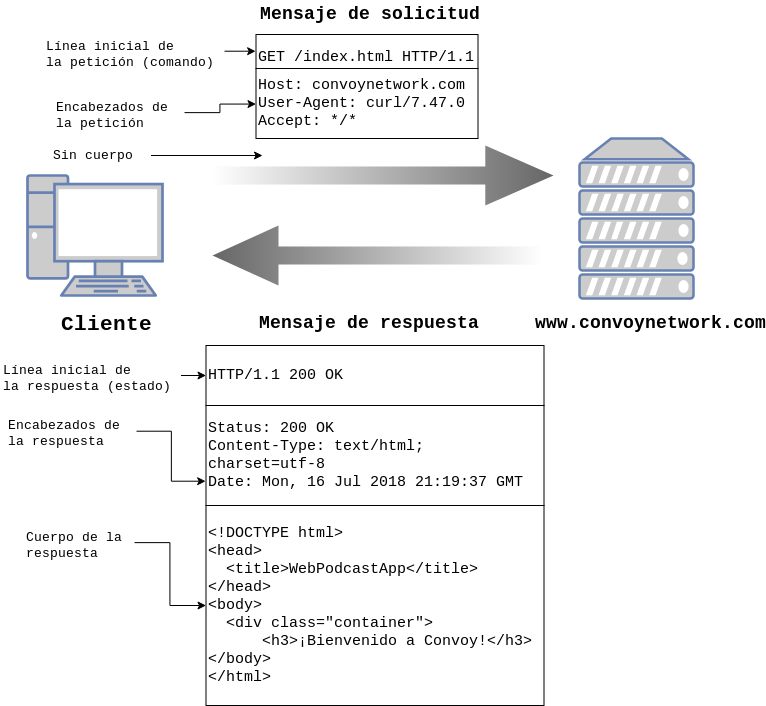
\includegraphics[scale=0.5]{figures/http_message.png}
    \caption{Ejemplo de la estructura de un mensaje de solicitud y de respuesta. El cliente solicita el archivo \texttt{index.html} mediante
    un \texttt{GET} y el servidor le regresa el archivo con un código de estado
    200.}
    \label{http-message}
\end{figure}

\end{description}


\subsection{World Wide Web}
\label{\detokenize{chapter_one/rest:world-wide-web}}
La World Wide Web o Web (Red Informática Mundial en español)  es un espacio de
información en el cual los objetos de interés, conocidos como \textit{recursos},
son identificados por Identificadores de Recursos Uniformes (URI por sus
siglas en inglés). En diciembre de 1990, Tim Bernes-Lee comenzó este proyecto,
donde inventó e implementó, entre otras cosas:
\begin{itemize}
\item {} 
El Identificador de Recursos Uniforme, una sintáxis que asigna a cada documento web una dirección única.

\item {} 
El Protocolo de Transferencia de Hipertexto (HTTP), un lenguaje basado en mensajes que las computadoras pueden usar para comunicarse a través de Internet.

\item {} 
El Lenguaje de Marcas de Hipertexto (HTML), para representar documentos informativos que contienen enlaces a documentos relacionados.

\item {} 
El primer servidor web.

\item {} 
El primer navegador web, llamado «Nexus».

\end{itemize}

Desde el momento que el proyecto se publicó, comenzó a crecer exponencialmente.
El tráfico de la web estaba superando la capacidad de la infraestructura del Internet.


\subsubsection{Arquitectura web}
\label{\detokenize{chapter_one/rest:arquitectura-web}}
A finales de 1993, Roy Fielding, a través de un análisis, reconoció que la escalabilidad
de la web estaba gobernada por un conjunto de restricciones clave.
Fielding agrupó en seis categorías esas restricciones y de manera manera colectiva
se refirió a ellas como el \sphinxstyleemphasis{estilo arquitectónico de la web}.


\paragraph{Cliente servidor}
\label{\detokenize{chapter_one/rest:cliente-servidor}}
La web es un sistema basado en la dupla cliente-servidor, en la cual clientes y servidores
tienen distintos papeles. Estos pueden ser implementados y desarrollados independientemente,
usando cualquier lenguaje o tecnología, con tal que de que se ajusten a la \sphinxstyleemphasis{interfaz uniforme de la web}.


\paragraph{Interfaz uniforme}
\label{\detokenize{chapter_one/rest:interfaz-uniforme}}
Las interacciones entre los componentes web (clientes, servidores e intermediarios),
dependen de la uniformidad en sus interfaces. Si cualesquiera de estos componentes se
salen de los estándares establecidos, entonces la comunicación en la web
se rompe.

Los componentes web interactúan consistentemente dentro las siguientes
cuatro restricciones de la interfaz uniforme.


\subparagraph{Identificación de recursos}
\label{\detokenize{chapter_one/rest:identificacion-de-recursos}}
Como se mencionó anteriormente, los elementos dentro de la web son
conocidos como \sphinxstyleemphasis{recursos} y tienen un identificador único. Por ejemplo, una
página web como \sphinxstyleemphasis{http://convoynetwork.com/}, identifica de manera única el
recurso en la raíz del sitio web.


\subparagraph{Manipulación de recursos a través de sus representaciones}
\label{\detokenize{chapter_one/rest:manipulacion-de-recursos-a-traves-de-sus-representaciones}}
Los clientes manipulan representaciones de recursos. Un mismo
recurso puede ser representado de diferentes formas a diferentes
clientes. Por ejemplo, un documentos puede representarse como un HTML
para un navegador web, y un JSON para un programa automatizado. La idea
principal es que la representación es una manera de interactuar con el recurso
pero no es el recurso en sí.


\subparagraph{Mensajes autodescriptivos}
\label{\detokenize{chapter_one/rest:mensajes-autodescriptivos}}
El estado deseado de un recurso puede ser representado dentro del mensaje
de petición del cliente. El estado actual de un recurso puede estar representado
dentro del mensaje de respuesta por parte del servidor.
Los mensajes autodescriptivos pueden incluir metadatos para comunicar
detalles adicionales con respecto al estado del recurso, el formato
de representacion y tamaño, y el mensaje mismo.
Un mensaje HTTP provee \sphinxstyleemphasis{encabezados} para organizar varios tipos de
de metadatos en campos uniformes.


\subparagraph{Hipermedia como el motor del estado de la aplicación (HATEOAS)}
\label{\detokenize{chapter_one/rest:hipermedia-como-el-motor-del-estado-de-la-aplicacion-hateoas}}
La representación del estado de un recurso incluye enlaces a recursos
relacionados. Los enlaces son los hilos que entrelazan la web, permitiendo
a los usuarios moverse a través de aplicaciones y datos de una manera directa
y significativa. La presencia, o ausencia, de un enlace en una página es una
parte importante del estado del recurso actual.


\paragraph{Sistema de capas}
\label{\detokenize{chapter_one/rest:sistema-de-capas}}
Las restricciones del sistema en capas permiten intermediarios de red como
los proxies y puertas de acceso sean desplegadas de manera transparente entre el cliente
y el servidor usando una interfaz uniforme de la web. Intermediarios basados
en la red se usan para reforzar la seguridad, almacenamiento en caché de
respuestas, y balanceo de carga.


\paragraph{Caché}
\label{\detokenize{chapter_one/rest:cache}}
El almacenamiento en caché es una de las restricciones más importantes de la
arquitectura de la web. Las restricciones de la caché dan órdenes a un servidor
web para declarar la \sphinxstyleemphasis{cacheabilidad} de cada datos de la respuesta.
Guardar en la caché datos de la respuesta pueden ayudar a reducir
la latencia percibida por el cliente, aumentar la disponibilidad
general y confiabilidad de una aplicación, y controlar la carga
de un servidor web. En resumen, el almacenamiento en caché
reduce el \sphinxstyleemphasis{costo} general de la Web.


\paragraph{Stateless}
\label{\detokenize{chapter_one/rest:stateless}}
La restricción stateless dicta que un servidor web no está obligado
a memorizar el estado de sus aplicaciones cliente. Como resultado,
cada cliente debe incluir toda la información contextual que considere
sea relevante en cada interacción con el servidor web. Los servidores
web solicitan a los clientes administrar la complejidad de comunicar
el estado de su aplicación tal que el servidor web puede servir a un número
mayor de clientes.


\paragraph{Código bajo demanda}
\label{\detokenize{chapter_one/rest:codigo-bajo-demanda}}
Esta restricción permite a los servidores web transferir temporalmente
programas ejecutables, tales como scripts o extensiones a los cliente.
El código bajo demanda tiende a establecer un acoplamiento de tecnología
entre servidores web y sus clientes, ya que el cliente debe tener la habilidad
de entender y ejecutar el código que descarga cuando lo desea desde el servidor.
Por esta razón, el código bajo demanda es la única restricción del
estilo arquitectónico de la web que se considera opcional.


\subsection{Transferencia de Estado Representacional (REST)}
\label{\detokenize{chapter_one/rest:transferencia-de-estado-representacional-rest}}
En el año 2000, después de que la crisis de la escalabilidad de la web se
evitó, Fielding llamó y describió al estilo arquitectónico de la web en su
trabajo doctoral. \sphinxstylestrong{Transferencia de Estado Representacional} (REST por
sus siglas en inglés) fue el nombre que Fielding dio a su descripción del
estilo arquitectónico de la web, que está compuesto por las restricciones
mencionadas previamente.

La Transferencia de Estado Representacional es un estilo de arquitectura de software.
Este estilo es
una abstracción de elementos arquitectónicos dentro de un sistema de hipermedia
distribuido como es la Web. REST ignora los detalles de la implementación de
componentes y sintaxis de protocolos de manera que pueda enfocarse en los
papeles de los componentes, las restricciones sobre su interacción con otros
componentes, y la interpretación de elementos de datos significativos.
Abarca las limitaciones fundamentales sobre los componentes, conectores y datos
que definen las bases de la arquitectura web y, por lo tanto, la esencia de su
comportamiento como una aplicación basada en red. REST no es un estándar, sin
embargo sí un conjunto de restricciones. No está atado al protocolo HTTP,
pero a menudo se asocia con éste.


\subsubsection{API REST}
\label{\detokenize{chapter_one/rest:api-rest}}
Un \sphinxstyleemphasis{servicio web} es un sistema de software diseñado para admitir
la interacción interoperable de una máquina a otra  máquina a través de una red.
Programas cliente usan \sphinxstyleemphasis{interfaces de programación de aplicaciones} (API
por sus siglas en inglés) para comunicarse con servicios web. Generalmente
hablando, una API expone un conjunto de datos y funciones para facilitar
interacciones entre programas de computadora y permitiendo que
intercambien información.

\begin{figure}[htbp]
\centering
\capstart

\noindent\sphinxincludegraphics[scale=0.60]{{web_service_cycle}.png}
\caption{Una API web es el frente de un servicio web, escuchando y respondiendo las peticiones de los cliente directamente.}\label{\detokenize{chapter_one/rest:web-service-cycle}}\end{figure}

El estilo arquitectónico REST se aplica comúnmente al diseño de API para
servicios web modernos. Una API web que sigue el estilo REST es una API REST.
Tener una API REST hace a un servicio web RESTful. Una API REST está formada de
recursos entrelazados.

\begin{remark}
REST es una arquitectura basada en recursos. Se accede a un recurso a través
de una interfaz común basada en los métodos estándar de HTTP. REST
solicita a los desarrolladores usar métodos HTTP explícitamente
y de una forma que sea consistente con la definción del protocolo.
Cada recurso se identifica con un URL. Todos los recursos deben soportar
las operaciones HTTP más comunes, además REST permite que ese recurso
tenga diferentes representaciones, por ejemplo, texto, xml, json, etc.
El cliente REST puede solicitar una representacion en específico por
medio del protocolo HTTP. La \hyperref[\detokenize{chapter_one/rest:rest-struct}]{Tabla \ref{\detokenize{chapter_one/rest:rest-struct}}} describe
los elementos usados en REST.
\end{remark}


\begin{savenotes}\sphinxattablestart
\centering
\sphinxcapstartof{table}
\sphinxcaption{Elementos de REST}\label{\detokenize{chapter_one/rest:rest-struct}}
\sphinxaftercaption
\begin{tabulary}{\linewidth}[t]{|T|T|}
\hline
\sphinxstylethead{ 
Elemento
\unskip}\relax &\sphinxstylethead{ 
Descripción
\unskip}\relax \\
\hline
Recurso
&
Objetivo conceptual de una referencia de hipertexto. Por ejemplo: podcast.
\\
\hline
Identificador de recurso
&
Un URL que identifica un recurso en específico. Por ejemplo: \sphinxurl{http://convoynetwork.com/podcast/123}
\\
\hline
Metadatos del recurso
&
Información que describe al recurso. Por ejemplo: autor, etiqueta, etc.
\\
\hline
Representación
&
El contenido del recurso. Por ejemplo: un JSON, un HTML o una imagen JPEG.
\\
\hline
Metadatos de la representación
&
Información que describe como procesar la representación. Por ejemplo: tipo de medio, fecha, etc.
\\
\hline
Datos de control
&
Información que describe cómo optimizar el procesamiento de respuesta. Por ejemplo: if-modified-since, cache-control-expiry.
\\
\hline
\end{tabulary}
\par
\sphinxattableend\end{savenotes}


% 
\section{Servicios de BaaS y Firebase}
\label{\detokenize{chapter_one/firebase:servicios-de-baas-y-firebase}}\label{\detokenize{chapter_one/firebase::doc}}

\subsection{Backend as a Service}
\label{\detokenize{chapter_one/firebase:backend-as-a-service}}

\begin{remark}
Backend as a service o Mobile Backend as a Service, es un
modelo para proporcionar a los desarrolladores web y
de aplicaciones móviles una forma de vincular estas aplicaciones
al almacenamiento en la nube, servicios analíticos
y/o otras características tales como la gestión de usuarios,
la posibilidad de enviar notificaciones push y la integración
con servicios de redes sociales. Estos servicios son brindados
a través de kits de desarrollo de software (SDK) o
interfaces de programación de aplicaciones (API). 
\end{remark}
Algunos proveedores
de este tipo de cómputo en la nube son Microsoft Azure Mobile Services,
Oracle Cloud (Mobile Service) y \sphinxstylestrong{Firebase}, que es la plataforma
que se usa en este proyecto y por tanto se describe a detalle a
continuación.


\subsection{Firebase}
\label{\detokenize{chapter_one/firebase:firebase}}
Firebase es una plataforma de desarrollo para aplicaciones móviles y web.
Tiene varias tecnologías para mejorar la experiencia de desarrollo de una
aplicación, como la autenticación, base de datos en tiempo real,
almacenamiento en la nube, alojamiento de un sitio estático y funciones en la
nube para ejecutar código de backend.

A pesar de ser una plataforma enfocada principalmente para ser un servicio de
backend para aplicaciones móviles y web, algunos de sus servicios cuentan con
una API REST lo que permite acceder a estos a través de entornos con recursos
restringidos.

De las tecnologías ofrecidas por Firebase, se usan:
\begin{itemize}
\item {} 
Realtime database

\item {} 
Authentication

\item {} 
Hosting

\end{itemize}


\subsubsection{Firebase Realtime Database}
\label{\detokenize{chapter_one/firebase:firebase-realtime-database}}
Firebase Realtime Database es una base de datos alojada en la nube.
Los datos se almacenan en formato JSON y se sincronizan en tiempo real con cada
cliente conectado. Los clientes comparten una instancia de Realtime Database y
reciben actualizaciones automáticamente con los datos más recientes.

Entre las funciones más importantes de este servicio están; la
\sphinxstylestrong{sincronización de datos en tiempo real}, cada vez que los datos cambian,
los dispositivos conectados reciben esa actualización en milisegundos.
Trabajo \sphinxstylestrong{sin conexión}, ya que el SDK hace que los datos persistan en el disco,
y cuando la conexión se restablece, el dispositivo cliente recibe los cambios
faltantes y los sincroniza con el estado actual del servidor.
\sphinxstylestrong{Accesible desde dispositivos cliente}, no se necesita un servidor de
aplicaciones; las opciones de seguridad y validación se definen a través de
reglas de seguridad de Firebase Realtime Database. Y finalmente
el \sphinxstylestrong{escalamiento en varias bases de datos}, que permite dividir la información
en diversas instancias de bases de datos dentro del mismo proyecto de Firebase.

La ruta de implementación de la Realtime Database que está definida en la documentación de Firebase,
es la siguiente:
\begin{enumerate}
\item {} 
Integrar los SDK de Firebase Realtime Database.

\item {} 
Crear referencias de Realtime Database.

\item {} 
Configurar datos y escuchar para detectar cambios.

\item {} 
Habilitar la persistencias sin conexión.

\item {} 
Proteger los datos con las reglas de seguridad de Firebase Realtime Database.

\end{enumerate}


\subsubsection{Firebase Authentication}
\label{\detokenize{chapter_one/firebase:firebase-authentication}}
La mayoría de las aplicaciones necesitan identificar a los usuarios. Conocer la
identidad de un usuario permite que una aplicación guarde sus datos en la nube de
forma segura y proporcione la misma experiencia personalizada en todos los
dispositivos del usuario.

Firebase Authentication proporciona servicios de backend, SDK fáciles de usar y
bibliotecas de IU ya elaboradas para autenticar a los usuarios en tu aplicación.
Admite la autenticación mediante contraseñas, números de teléfono, proveedores
de identidad federados populares, como Google, Facebook y Twitter, y mucho más.

Firebase Authentication se integra estrechamente con otros servicios de Firebase
y aprovecha los estándares de la industria como OAuth 2.0 y OpenID Connect, por
lo que se puede integrar fácilmente con tu backend personalizado.


\paragraph{FirebaseUI Auth}
\label{\detokenize{chapter_one/firebase:firebaseui-auth}}
Puedes permitir que los usuarios accedan a tu aplicación de Firebase con FirebaseUI
como solución de autenticación directa o mediante el SDK de Firebase
Authentication para integrar de forma manual uno o más métodos de acceso en tu
aplicación.

FirebaseUI proporciona una solución de autenticación directa que controla los
flujos de IU para los usuarios que acceden con direcciones de correo electrónico
y contraseñas, números de teléfono y con proveedores de identidad federada
populares, que incluyen el Acceso con Google y el Acceso con Facebook.

El componente de FirebaseUI Auth implementa recomendaciones para la autenticación
en sitios web y dispositivos móviles, lo que puede maximizar la conversión de
acceso y registro de tu aplicación. También maneja casos extremos, como recuperación
y vinculación de cuentas, que pueden tener repercusiones en la seguridad y ser
propensos a generar errores cuando se tratan de manejar correctamente.



\subsubsection{Firebase Hosting}
\label{\detokenize{chapter_one/firebase:firebase-hosting}}
Firebase Hosting proporciona hosting estático, rápido y seguro para tu aplicación web.

Firebase Hosting es un servicio de hosting de contenido web con nivel de
producción orientado a programadores. Con Hosting, puedes implementar aplicaciones web
y contenido estático en una red de distribución de contenido global (CDN) con
un solo comando, en forma rápida y sencilla.


\paragraph{Ruta de implementación}
\label{\detokenize{chapter_one/firebase:ruta-de-implementacion}}\begin{enumerate}
\item {} 
Instala Firebase CLI. Con Firebase CLI, es fácil configurar un nuevo proyecto de Hosting, administrar un servidor de desarrollo local y también implementar contenido

\item {} 
Configura un directorio de proyectos. Agrega archivos para tu aplicación web y agrega tus activos estáticos a tu carpeta local de Hosting. A continuación, puedes ejecutar \sphinxcode{firebase serve} para tu sitio en forma local.

\item {} 
Implementa tu sitio. Cuando estés satisfecho con la configuración, ejecuta \sphinxcode{firebase deploy} para subir la última instantánea a nuestros servidores.

\end{enumerate}
% 


\section{Interfaces de Programación de Aplicaciones de Transferencia de Estado Representacional}
\label{\detokenize{chapter_one/apis_rest:interfaces-de-programacion-de-aplicaciones-de-transferencia-de-estado-representacional}}\label{\detokenize{chapter_one/apis_rest::doc}}
Para entender mejor el concepto de una API REST conviene poner como ejemplos
los servicios web RESTful que se utilizan en este proyecto. Se accede
a esos servicios a través de sus API REST y se enlistan a continuación:
\begin{itemize}
\item {} 
Google Cloud Vision

\item {} 
Kairos

\item {} 
Wit.ai

\item {} 
Firebase Realtime Database

\end{itemize}


\subsection{API de Google Cloud Vision}
\label{\detokenize{chapter_one/apis_rest:api-de-google-cloud-vision}}
La API Vision de Google Cloud permite que los desarrolladores comprendan el
contenido de una imagen mediante el encapsulado de potentes modelos de
aprendizaje automático en una API REST fácil de usar. La API clasifica
imágenes rápidamente en miles de categorías (por ejemplo, «barco de vela»,
«león» o «torre Eiffel»), detecta objetos y caras individuales dentro de las
imágenes, además de buscar y leer palabras impresas en ellas.

El recurso que se solicita para el procesamiento de imagenes es \sphinxcode{images} y
el URL que lo identifica es \sphinxcode{https://vision.googleapis.com/v1/images:annotate}.
La API únicamente tiene definida la operación con el método HTTP POST,
por lo que hacer un POST a la URL del recurso ejecuta la detección de algunas
características en una o varias imágenes.

El cuerpo del mensaje del petición HTTP es un JSON con la siguente estructura
(por simplicidad se omiten varios objetos del JSON que no se utilizaron en el
proyecto):

\begin{sphinxVerbatim}[commandchars=\\\{\}]
\PYG{p}{\PYGZob{}}
  \PYG{l+s+s2}{\PYGZdq{}requests\PYGZdq{}} \PYG{o}{:} \PYG{p}{[}
    \PYG{p}{\PYGZob{}}
      \PYG{l+s+s2}{\PYGZdq{}image\PYGZdq{}} \PYG{o}{:} \PYG{p}{\PYGZob{}}
        \PYG{l+s+s2}{\PYGZdq{}content\PYGZdq{}} \PYG{o}{:} \PYG{n+nx}{string}\PYG{p}{,}
        \PYG{l+s+s2}{\PYGZdq{}source\PYGZdq{}} \PYG{o}{:} \PYG{p}{\PYGZob{}}
          \PYG{l+s+s2}{\PYGZdq{}gcsImageUri\PYGZdq{}} \PYG{o}{:} \PYG{n+nx}{string}\PYG{p}{,}
          \PYG{l+s+s2}{\PYGZdq{}imageUri\PYGZdq{}} \PYG{o}{:} \PYG{n+nx}{string}
        \PYG{p}{\PYGZcb{}}
      \PYG{p}{\PYGZcb{}}
      \PYG{l+s+s2}{\PYGZdq{}features\PYGZdq{}} \PYG{o}{:} \PYG{p}{[}
        \PYG{p}{\PYGZob{}}
          \PYG{l+s+s2}{\PYGZdq{}type\PYGZdq{}} \PYG{o}{:} \PYG{n+nx}{string}\PYG{p}{,}
          \PYG{l+s+s2}{\PYGZdq{}maxResults\PYGZdq{}} \PYG{o}{:} \PYG{n+nx}{number}
        \PYG{p}{\PYGZcb{}}
      \PYG{p}{]}
    \PYG{p}{\PYGZcb{}}
  \PYG{p}{]}
\PYG{p}{\PYGZcb{}}
\end{sphinxVerbatim}

\sphinxcode{requests} es una lista de objetos, donde cada objeto representa una imagen
y las caracterísiticas que se piden detectar. \sphinxcode{image} es la representación
de la imagen, que puede estar en tres formas distintas: codificada en base 64,
guardada en el servicio de almacenamiento en la nuble de Google Cloud Storage
o a través de un enlace en algún servidor. Para el primer caso a \sphinxcode{content}
se le asigna la image codificada; en cambio, si está en un contenedor de Google Cloud Storage
entonces se pasa a \sphinxcode{gcsImageUri} el valor de la URL de la imagen. Si se encuentra
en algún otro servicio de almacenamiento simplemente el valor de \sphinxcode{imageUri}
es el URL de la imagen.

\sphinxcode{features} es un arreglo de las caracterísiticas que se pretenden reconocer
en la imagen. Por cada objeto se tiene \sphinxcode{type} que es el tipo de caracterísitica
y \sphinxcode{maxResults} que es el número máximo de ese tipo. \sphinxcode{type} puede tomar
los siguientes valores:
\begin{itemize}
\item {} 
\sphinxcode{TYPE\_UNSPECIFIED}: No se específica la característica.

\item {} 
\sphinxcode{FACE\_DETECTION}: Ejecuta la detección de rostros.

\item {} 
\sphinxcode{LANDMARK\_DETECTION}: Ejecuta la detección de puntos de referencia.

\item {} 
\sphinxcode{LOGO\_DETECTION}: Ejecuta la detección de logotipos.

\item {} 
\sphinxcode{LABEL\_DETECTION}: Ejecuta la detección de etiquetas.

\item {} 
\sphinxcode{TEXT\_DETECTION}: Ejecuta el reconocimiento óptico de caracteres (OCR).

\item {} 
\sphinxcode{DOCUMENT\_TEXT\_DETECTION}: Ejecuta el OCR sobre grandes documentos de texto.

\item {} 
\sphinxcode{SAFE\_SEARCH\_DETECTION}: Ejecuta la búqueda segura para detectar contenido pontencialmente inseguro o no deseable.

\item {} 
\sphinxcode{IMAGE\_PROPERTIES}: Calcula un conjunto de propiedades en una imagen, como los colores dominantes.

\item {} 
\sphinxcode{CROP\_HINTS}: Ejecuta la sugerencia de recortes de una imagen.

\item {} 
\sphinxcode{WEB\_DETECTION}: Ejecuta la detección web.

\end{itemize}

De todas estas posibles caracterísiticas, las que se utilizan dentro de la arquitectura
CloudNAO son \sphinxcode{TEXT\_DETECTION} y \sphinxcode{LABEL\_DETECTION}.

El cuerpo del mensaje de respuesta, si todo salió bien (se obtiene una código
de estado 200), contiene información
con la siguiente estructura:

\begin{sphinxVerbatim}[commandchars=\\\{\}]
\PYG{p}{\PYGZob{}}
  \PYG{l+s+s2}{\PYGZdq{}responses\PYGZdq{}}\PYG{o}{:} \PYG{p}{[}
    \PYG{p}{\PYGZob{}}
        \PYG{l+s+s2}{\PYGZdq{}labelAnnotations\PYGZdq{}}\PYG{o}{:} \PYG{p}{[}
          \PYG{p}{\PYGZob{}}
            \PYG{l+s+s2}{\PYGZdq{}mid\PYGZdq{}}\PYG{o}{:} \PYG{n+nx}{string}\PYG{p}{,}
            \PYG{l+s+s2}{\PYGZdq{}description\PYGZdq{}}\PYG{o}{:} \PYG{n+nx}{string}\PYG{p}{,}
            \PYG{l+s+s2}{\PYGZdq{}score\PYGZdq{}}\PYG{o}{:} \PYG{n+nx}{number}
          \PYG{p}{\PYGZcb{}}
        \PYG{p}{]}\PYG{p}{,}
        \PYG{l+s+s2}{\PYGZdq{}textAnnotations\PYGZdq{}}\PYG{o}{:} \PYG{p}{[}
          \PYG{p}{\PYGZob{}}
              \PYG{l+s+s2}{\PYGZdq{}mid\PYGZdq{}}\PYG{o}{:} \PYG{n+nx}{string}\PYG{p}{,}
              \PYG{l+s+s2}{\PYGZdq{}locale\PYGZdq{}}\PYG{o}{:} \PYG{n+nx}{string}\PYG{p}{,}
              \PYG{l+s+s2}{\PYGZdq{}score\PYGZdq{}}\PYG{o}{:} \PYG{n+nx}{number}\PYG{p}{,}
              \PYG{l+s+s2}{\PYGZdq{}boundingPoly\PYGZdq{}}\PYG{o}{:} \PYG{p}{\PYGZob{}}
                \PYG{l+s+s2}{\PYGZdq{}vertices\PYGZdq{}}\PYG{o}{:} \PYG{p}{[}
                  \PYG{p}{\PYGZob{}}
                    \PYG{l+s+s2}{\PYGZdq{}x\PYGZdq{}}\PYG{o}{:} \PYG{n+nx}{number}\PYG{p}{,}
                    \PYG{l+s+s2}{\PYGZdq{}y\PYGZdq{}}\PYG{o}{:} \PYG{n+nx}{number}
                  \PYG{p}{\PYGZcb{}}
                \PYG{p}{]}
              \PYG{p}{\PYGZcb{}}
          \PYG{p}{\PYGZcb{}}
        \PYG{p}{]}
    \PYG{p}{\PYGZcb{}}
  \PYG{p}{]}
\PYG{p}{\PYGZcb{}}
\end{sphinxVerbatim}

La respuesta obtenida depende de qué caracterísiticas se solicitaron. Para el JSON anterior suponemos que se pidió la detección de
categorías y el reconocimiento de texto. \sphinxcode{mid} es un identificador,
\sphinxcode{description} es la descripción textual de la entidad; por ejemplo,
para el caso de \sphinxcode{labelAnnotations}, \sphinxcode{description} puede tener un valor
asociado igual a «psychedelic art», en cambio para \sphinxcode{textAnnotations},
se espera tenga una cadena del texto encontrado como «lateralus».

El \sphinxcode{score} es la precisión de la detección de la entidad en la imagen,
toma valores en el intervalo {[}0, 1{]}. \sphinxcode{boundingPoly} contiene
las coordenadas del polígono que encierra la entidad encontrada.


\subsection{API de Kairos}
\label{\detokenize{chapter_one/apis_rest:api-de-kairos}}
Kairos permite a los desarrolladores integrar un análisis de rostros preciso
y rápido en cualquier aplicación o servicio. Cuenta con un API REST
para ejecutar tareas en la nube como la detección e identificación de rostros,
emociones, raza, edad, entre otras. También cuenta con un SDK, más limitado
pero que puede ejecutarse offline y directamente en dispositivos móviles.
En esta sección se describe cómo se debe hacer una petición
y cuál es la repuesta que retorna el servicio.
% Por ahora sólo nos interesa la API REST, por lo que describiremos cómo funciona,
% es decir, cómo se debe hacer una petición y cuál es la respuesta
% que envía el servicio.

Para realizar el reconocimiento de caras, la API tiene como URL base
\sphinxcode{https://api.kairos.com} y cuenta con diversos recursos para cada tipo de
reconocimiento. Únicamente nos interesan dos recursos, \sphinxcode{enroll} y
\sphinxcode{recognize}, que son relativos al URL base.
El primero toma una fotografía, encuentra rostros en esta,
y los guarda en una galería, cada rostro necesita un identificador de la
persona. Las galerías sirven para que posteriormente se reconozca a un sujeto
por medio de su fotografía.

El otro recurso que nos interesa es \sphinxcode{recognize}, que toma una fotografía,
encuentra caras e intenta emparejarlas con las que sean guardado
previamente en una galería.

Para hacer ambas peticiones se utiliza el método POST. Al hacer un POST
a \sphinxcode{enroll} se debe enviar un JSON con la siguiente estructura en el cuerpo
del mensaje.

\begin{sphinxVerbatim}[commandchars=\\\{\}]
\PYG{p}{\PYGZob{}}
  \PYG{l+s+s2}{\PYGZdq{}image\PYGZdq{}}\PYG{o}{:} \PYG{n+nx}{string}\PYG{p}{,}
  \PYG{l+s+s2}{\PYGZdq{}subject\PYGZus{}id\PYGZdq{}}\PYG{o}{:} \PYG{n+nx}{string}\PYG{p}{,}
  \PYG{l+s+s2}{\PYGZdq{}gallery\PYGZus{}name\PYGZdq{}}\PYG{o}{:} \PYG{n+nx}{string}
\PYG{p}{\PYGZcb{}}
\end{sphinxVerbatim}

\sphinxcode{image} es un URL de acceso público o la codificación en base 64, \sphinxcode{subject\_id} es un identificador
de una cara, es único y es definido por el desarrollador, \sphinxcode{gallery\_name}
definida también por el desarrollador sirve para identificar la galería.

La respuesta de un POST a \sphinxcode{/enroll}, si todo fue exitoso
es un JSON con la siguiente estructura.

\begin{sphinxVerbatim}[commandchars=\\\{\}]
\PYG{p}{\PYGZob{}}\PYG{l+s+s2}{\PYGZdq{}face\PYGZus{}id\PYGZdq{}}\PYG{o}{:} \PYG{n+nx}{string}\PYG{p}{,}
  \PYG{l+s+s2}{\PYGZdq{}images\PYGZdq{}}\PYG{o}{:} \PYG{p}{[}
    \PYG{p}{\PYGZob{}}
      \PYG{l+s+s2}{\PYGZdq{}attributes\PYGZdq{}}\PYG{o}{:} \PYG{p}{\PYGZob{}}
        \PYG{l+s+s2}{\PYGZdq{}lips\PYGZdq{}}\PYG{o}{:} \PYG{n+nx}{string}\PYG{p}{,}
        \PYG{l+s+s2}{\PYGZdq{}asian\PYGZdq{}}\PYG{o}{:} \PYG{n+nx}{number}\PYG{p}{,}
        \PYG{l+s+s2}{\PYGZdq{}gender\PYGZdq{}}\PYG{o}{:} \PYG{p}{\PYGZob{}}
          \PYG{l+s+s2}{\PYGZdq{}type\PYGZdq{}}\PYG{o}{:} \PYG{n+nx}{string}
        \PYG{p}{\PYGZcb{}}\PYG{p}{,}
        \PYG{l+s+s2}{\PYGZdq{}age\PYGZdq{}}\PYG{o}{:} \PYG{n+nx}{number}\PYG{p}{,}
        \PYG{l+s+s2}{\PYGZdq{}hispanic\PYGZdq{}}\PYG{o}{:} \PYG{n+nx}{number}\PYG{p}{,}
        \PYG{l+s+s2}{\PYGZdq{}other\PYGZdq{}}\PYG{o}{:} \PYG{n+nx}{number}\PYG{p}{,}
        \PYG{l+s+s2}{\PYGZdq{}black\PYGZdq{}}\PYG{o}{:} \PYG{n+nx}{number}\PYG{p}{,}
        \PYG{l+s+s2}{\PYGZdq{}white\PYGZdq{}}\PYG{o}{:} \PYG{n+nx}{number}\PYG{p}{,}
        \PYG{l+s+s2}{\PYGZdq{}glasses\PYGZdq{}}\PYG{o}{:} \PYG{n+nx}{string}
      \PYG{p}{\PYGZcb{}}\PYG{p}{,}
      \PYG{l+s+s2}{\PYGZdq{}transaction\PYGZdq{}}\PYG{o}{:} \PYG{p}{\PYGZob{}}
        \PYG{l+s+s2}{\PYGZdq{}status\PYGZdq{}}\PYG{o}{:} \PYG{n+nx}{string}\PYG{p}{,}
        \PYG{l+s+s2}{\PYGZdq{}topLeftX\PYGZdq{}}\PYG{o}{:} \PYG{n+nx}{number}\PYG{p}{,}
        \PYG{l+s+s2}{\PYGZdq{}topLeftY\PYGZdq{}}\PYG{o}{:} \PYG{n+nx}{number}\PYG{p}{,}
        \PYG{l+s+s2}{\PYGZdq{}gallery\PYGZus{}name\PYGZdq{}}\PYG{o}{:} \PYG{n+nx}{string}\PYG{p}{,}
        \PYG{l+s+s2}{\PYGZdq{}timestamp\PYGZdq{}}\PYG{o}{:} \PYG{n+nx}{string}\PYG{p}{,}
        \PYG{l+s+s2}{\PYGZdq{}height\PYGZdq{}}\PYG{o}{:} \PYG{n+nx}{number}\PYG{p}{,}
        \PYG{l+s+s2}{\PYGZdq{}quality\PYGZdq{}}\PYG{o}{:} \PYG{n+nx}{number}\PYG{p}{,}
        \PYG{l+s+s2}{\PYGZdq{}confidence\PYGZdq{}}\PYG{o}{:} \PYG{n+nx}{number}\PYG{p}{,}
        \PYG{l+s+s2}{\PYGZdq{}subject\PYGZus{}id\PYGZdq{}}\PYG{o}{:} \PYG{n+nx}{string}\PYG{p}{,}
        \PYG{l+s+s2}{\PYGZdq{}width\PYGZdq{}}\PYG{o}{:} \PYG{n+nx}{number}\PYG{p}{,}
        \PYG{l+s+s2}{\PYGZdq{}face\PYGZus{}id\PYGZdq{}}\PYG{o}{:} \PYG{n+nx}{number}
      \PYG{p}{\PYGZcb{}}
    \PYG{p}{\PYGZcb{}}\PYG{p}{]}\PYG{p}{\PYGZcb{}}
\end{sphinxVerbatim}

Para el caso
del POST a \sphinxcode{/recognize}, el cuerpo de la petición lleva un JSON como el
siguiente:

\begin{sphinxVerbatim}[commandchars=\\\{\}]
\PYG{p}{\PYGZob{}}
  \PYG{l+s+s2}{\PYGZdq{}image\PYGZdq{}}\PYG{o}{:} \PYG{n+nx}{string}\PYG{p}{,}
  \PYG{l+s+s2}{\PYGZdq{}gallery\PYGZus{}name\PYGZdq{}}\PYG{o}{:} \PYG{n+nx}{string}
\PYG{p}{\PYGZcb{}}
\end{sphinxVerbatim}

La respuesta enviada por Kairos,  si todo fue exitoso,
es un JSON con campos autodescriptivos como los
de la respuesta del recurso previo. Este JSON se muestra a continuación.

\begin{sphinxVerbatim}[commandchars=\\\{\}]
\PYG{p}{\PYGZob{}}
  \PYG{l+s+s2}{\PYGZdq{}images\PYGZdq{}}\PYG{o}{:} \PYG{p}{[}
    \PYG{p}{\PYGZob{}}
      \PYG{l+s+s2}{\PYGZdq{}transaction\PYGZdq{}}\PYG{o}{:} \PYG{p}{\PYGZob{}}
        \PYG{l+s+s2}{\PYGZdq{}status\PYGZdq{}}\PYG{o}{:} \PYG{n+nx}{string}\PYG{p}{,}
        \PYG{l+s+s2}{\PYGZdq{}width\PYGZdq{}}\PYG{o}{:} \PYG{n+nx}{number}\PYG{p}{,}
        \PYG{l+s+s2}{\PYGZdq{}topLeftX\PYGZdq{}}\PYG{o}{:} \PYG{n+nx}{number}\PYG{p}{,}
        \PYG{l+s+s2}{\PYGZdq{}topLeftY\PYGZdq{}}\PYG{o}{:} \PYG{n+nx}{number}\PYG{p}{,}
        \PYG{l+s+s2}{\PYGZdq{}gallery\PYGZus{}name\PYGZdq{}}\PYG{o}{:} \PYG{n+nx}{string}\PYG{p}{,}
        \PYG{l+s+s2}{\PYGZdq{}face\PYGZus{}id\PYGZdq{}}\PYG{o}{:} \PYG{n+nx}{number}\PYG{p}{,}
        \PYG{l+s+s2}{\PYGZdq{}confidence\PYGZdq{}}\PYG{o}{:} \PYG{n+nx}{number}\PYG{p}{,}
        \PYG{l+s+s2}{\PYGZdq{}subject\PYGZus{}id\PYGZdq{}}\PYG{o}{:} \PYG{n+nx}{string}\PYG{p}{,}
        \PYG{l+s+s2}{\PYGZdq{}height\PYGZdq{}}\PYG{o}{:} \PYG{n+nx}{number}\PYG{p}{,}
        \PYG{l+s+s2}{\PYGZdq{}quality\PYGZdq{}}\PYG{o}{:} \PYG{n+nx}{number}
      \PYG{p}{\PYGZcb{}}\PYG{p}{,}
      \PYG{l+s+s2}{\PYGZdq{}candidates\PYGZdq{}}\PYG{o}{:} \PYG{p}{[}
        \PYG{p}{\PYGZob{}}
          \PYG{l+s+s2}{\PYGZdq{}subject\PYGZus{}id\PYGZdq{}}\PYG{o}{:} \PYG{n+nx}{string}\PYG{p}{,}
          \PYG{l+s+s2}{\PYGZdq{}confidence\PYGZdq{}}\PYG{o}{:} \PYG{n+nx}{number}\PYG{p}{,}
          \PYG{l+s+s2}{\PYGZdq{}enrollment\PYGZus{}timestamp\PYGZdq{}}\PYG{o}{:} \PYG{n+nx}{string}
        \PYG{p}{\PYGZcb{}}\PYG{p}{,}
        \PYG{p}{\PYGZob{}}
          \PYG{l+s+s2}{\PYGZdq{}subject\PYGZus{}id\PYGZdq{}} \PYG{o}{:} \PYG{n+nx}{string}\PYG{p}{,}
          \PYG{l+s+s2}{\PYGZdq{}confidence\PYGZdq{}} \PYG{o}{:} \PYG{n+nx}{numref}\PYG{p}{,}
          \PYG{l+s+s2}{\PYGZdq{}enrollment\PYGZus{}timestamp\PYGZdq{}}\PYG{o}{:} \PYG{n+nx}{string}
        \PYG{p}{\PYGZcb{}}
      \PYG{p}{]}
    \PYG{p}{\PYGZcb{}}
  \PYG{p}{]}
\PYG{p}{\PYGZcb{}}
\end{sphinxVerbatim}


\subsection{API de Wit.ai}
\label{\detokenize{chapter_one/apis_rest:api-de-wit-ai}}
Wit.ai es una API para procesamiento de lenguaje natural capaz de convertir
oraciones en datos estructurados. Esto quiere decir que puedes crear bots
que interactúen con humanos en plataformas de mensajería. Con Wit.ai los
desarrolladores pueden contruir aplicaciones a las que se les pueda hablar o
escribir. Los bots aprenden conforme se les hable, se vuelven más inteligentes
en cada interacción.

Wit.ai, como muchos servicios, cuenta con diferentes SDK para lenguajes como
JavaScript, Python y Ruby. También tiene una API REST para extraer el significado
de una sentencia o de un discurso de audio. Por ahora nos enfocaremos
al segundo caso, cómo solicitar y cuál es la respuesta al enviar audio
para su procesamiento.

Wit trabaja con \sphinxstyleemphasis{intenciones} y \sphinxstyleemphasis{entidades}. Las intenciones se usan para entender
el significado en general de una oración. Por ejemplo la intención
de la oración «¿A qué hora abren la bibloteca central de CU?»
puede ser las horas de apertura de un lugar. Las entidades
proveen más información para contestar correctamente. Siguiendo el ejemplo,
el usuario no está preguntando a qué hora abren todas las bibliotecas,
sino en específico la biblioteca central de CU, por lo que
una entidad sería el lugar del que se desear obtener la hora de apertura.

La API cuenta con el URL base \sphinxcode{htttps://api.wit.ai/} y el recurso que
solicitamos es \sphinxcode{/speech}. A través de un POST a \sphinxcode{htttps://api.wit.ai/speech}
podemos obtener el significado de un archivo de audio.

A diferencia de las otras API donde no necesariamente tenemos que especificar
un encabezado en el mensaje de petición HTTP, aquí es necesario especificar
el formato del archivo de audio. Se debe pasar como valor al campo
\sphinxcode{Content-type} cualquiera de los siguientes:
\begin{itemize}
\item {} 
\sphinxcode{audio/wav}: si envias un archivo wav.

\item {} 
\sphinxcode{audio/mpeg3}: para un archivo mp3.

\item {} 
\sphinxcode{audio/ulaw}: para archivo G.11 u-law.

\end{itemize}

Wit.ai únicamente procesa audio en formato monoaural no estéreo.

En el cuerpo del mensaje va la información binaria, es decir,
el archivo de audio. La respuesta del servidor
es un JSON con la siguiente estructura:

\begin{sphinxVerbatim}[commandchars=\\\{\}]
\PYG{p}{\PYGZob{}}
  \PYG{l+s+s2}{\PYGZdq{}msg\PYGZus{}id\PYGZdq{}}\PYG{o}{:} \PYG{n+nx}{string}\PYG{p}{,}
  \PYG{l+s+s2}{\PYGZdq{}\PYGZus{}text\PYGZdq{}}\PYG{o}{:} \PYG{n+nx}{string}\PYG{p}{,}
  \PYG{l+s+s2}{\PYGZdq{}entities\PYGZdq{}}\PYG{o}{:} \PYG{p}{\PYGZob{}}
    \PYG{n+nx}{string} \PYG{o}{:} \PYG{p}{[} \PYG{p}{\PYGZob{}}
      \PYG{l+s+s2}{\PYGZdq{}value\PYGZdq{}}\PYG{o}{:} \PYG{n+nx}{string}\PYG{p}{,}
      \PYG{l+s+s2}{\PYGZdq{}confidence\PYGZdq{}}\PYG{o}{:} \PYG{n+nx}{number}
    \PYG{p}{\PYGZcb{}} \PYG{p}{]}\PYG{p}{,}
    \PYG{l+s+s2}{\PYGZdq{}intent\PYGZdq{}}\PYG{o}{:} \PYG{p}{\PYGZob{}}
      \PYG{l+s+s2}{\PYGZdq{}value\PYGZdq{}}\PYG{o}{:} \PYG{n+nx}{string}\PYG{p}{,}
      \PYG{l+s+s2}{\PYGZdq{}confidence\PYGZdq{}}\PYG{p}{;} \PYG{n+nx}{number}
    \PYG{p}{\PYGZcb{}}
  \PYG{p}{\PYGZcb{}}
\PYG{p}{\PYGZcb{}}
\end{sphinxVerbatim}

\sphinxcode{msg\_id} es el id de la respuesta. \sphinxcode{\_text} es la trancripción
del discurso de audio en texto. \sphinxcode{entities} es un objeto con las
entidades e intenciones que se encontraron. Si es una intención
el objeto tiene como llave la cadena \sphinxcode{"intent"} y como
valores los campos \sphinxcode{value} y \sphinxcode{confidence}, donde el primero
es el valor con el que se definió la intención y el segundo es la
probabilidad de que sea tal intención. Si es una
entidad la llave del objeto es el nombre de la entidad y como valor
tiene un arreglo de las diferentes apariciones que tiene
esa entidad en el mensaje. Cada entidad tiene los campos de
\sphinxcode{value} y \sphinxcode{confidence}.


\subsection{API REST de Firebase Database}
\label{\detokenize{chapter_one/apis_rest:api-rest-de-firebase-database}}
La base de datos en tiempo real de Firebase cuenta con una API REST
para realizar operaciones para leer, escribir, modificar o eliminar datos.

Se puede utilizar cualquier URL de la base de datos de Firebase como un endpoint
REST. Todo lo que se necesita es añadir la extensión \sphinxcode{.json} al final del
URL y enviar una petición desde cualquier cliente HTTP.

Para poder utilizar la API REST, el mapeo de los métodos
HTTP y las operaciones sobre Firebase Realtime Database es el siguiente.
\begin{itemize}
\item {} 
\sphinxstylestrong{GET}, para leer información previamente almacenada en la base de datos.

\item {} 
\sphinxstylestrong{PUT}, para escribir datos sobre una ubicación de la base de datos. Si existen datos los sobreescribe. Equivalente a \sphinxcode{set()} de los SDK.

\item {} 
\sphinxstylestrong{POST}, para añadir información en la base de datos. Se asigna un identificador único generado por Firebase. Es equivalente al \sphinxcode{push()} de los SDK.

\item {} 
\sphinxstylestrong{PATCH}, para actualizar datos en una ubicación sin sobreescribir. Equivalente a \sphinxcode{update()} de los SDK.

\item {} 
\sphinxstylestrong{DELETE}, elimina los datos en la ubicación dada.

\end{itemize}

La lista anterior muestra los métodos de lectura y escritura sobre la base
de datos, sin embargo, la API REST soportan el protocolo \sphinxstylestrong{Server-sent events (SSE)},
que define una API para recibir notificaciones push desde un servidor a través
de una conexión HTTP.

Para recibir las actualizaciones sobre una ubicación en la base de datos se
necesitan hacer tres cosas:
\begin{itemize}
\item {} 
Configurar el header \sphinxcode{Accept} igual a \sphinxcode{text/event-stream}. Del lado del cliente.

\item {} 
Respetar los redireccionamientos HTTP.

\item {} 
Si la ubicación de la base de datos requiere permisos, incluir el parámetro \sphinxcode{auth}.

\end{itemize}



En este capítulo se describieron algunos 
fundamentos teóricos y prácticos de la arquitectura de software 
propuesta. Se mencionó el funcionamiento de algunos elementos de los robots NAO y cómo se lleva a cabo el desarrollo de un programa
remota y localmente, el uso de los SDK para Java y Python y
ciertas API para manejar el movimiento del robot, la captura de 
video, imágenes y audio, etc. 

En el apartado de aprendizaje profundo se inicia con 
conceptos muy generales del aprendizaje automático,
se ahonda en las redes neuronales y el algoritmo de 
retropropagación para el aprendizaje de los parámetros
de una red y finalmente se describen las redes
convolucionales con un enfoque hacia la visión 
computacional. De TensorFlow, se describe 
la estructura fundamental de un programa usando esta
biblioteca y de los objetos que utiliza
para el entrenamiento y evaluación de un modelo, 
incluyendo un ejemplo, usando Python, de una
red neuronal que aprende la función XOR. 

En cuanto a las secciones de cómputo en la nube
y REST, se describieron algunos conceptos teóricos
de cada uno y las tecnologías que están involucradas.

De Firebase se mencionan a grandes rasgos 
tres características que ofrece y que se ocupan
en este proyecto, la base de datos en tiempo real,
el servicio de autenticanción y el servicio de alojamiento.
En el apartado de las API REST se describe cómo
se hacen solicitudes y cuáles son las respuestas
de los servicios de Google Cloud, Kairos y Wit.ai.

% %%%%%%%%%%%%%%%%%%%%%%%%%%%%%%%%%%%%%%%%%%%%%%%%%%%%%%%
% %%%%%%%%%%%%%%%%%%%%%%%%%%%%%%%%%%%%%%%%%%%%%%%%%%%%%%%
% %%%%%%%%%%%%%% Capítulo 2 : CloudNAO %%%%%%%%%%%%%%%%%%
% %%%%%%%%%%%%%%%%%%%%%%%%%%%%%%%%%%%%%%%%%%%%%%%%%%%%%%%
% %%%%%%%%%%%%%%%%%%%%%%%%%%%%%%%%%%%%%%%%%%%%%%%%%%%%%%%
\chapter{La arquitectura CloudNAO}
\label{\detokenize{chapter_two:la-arquitectura-cloudnao}}\label{\detokenize{chapter_two::doc}}
%%%%%%%%%%%%%%%%%%%%%%%%%%%%%%%%%%%%%%%%%%%%%%%%%%%%%%%%

En este capítulo se explica el desarrollo de la arquitectura de software CloudNAO y algunos casos de estudio donde utilizamos
algunos elementos de ésta.

En la Sección \ref{\detokenize{chapter_two/desc_cloudnao:descripcion-de-la-arquitectura-cloudnao}} se describen los componentes de
la arquitectura, como se comunican y relacionan entre ellos.
Esta sección incluye una subsección por cada elemento de CloudNAO
donde se agrega un apartado para usuarios y otro para desarrolladores.

En la Sección \ref{\detokenize{chapter_two/study_cases_implementation::doc}} se muestran tres casos de estudio, el primero es el 
reconocimiento rostros, el segundo incluye el reconocimiento
óptico de caracteres y su traducción y el tercer caso es
el reconocimiento de voz para que el robot realice ciertas
tareas.



% \section{Descripción de la arquitectura CloudNAO}
\label{\detokenize{chapter_two/desc_cloudnao:descripcion-de-la-arquitectura-cloudnao}}\label{\detokenize{chapter_two/desc_cloudnao::doc}}
CloudNAO integra servicios web de
terceros, servicios web desarrollados por el LAR, una aplicación móvil para
dispositivos con el sistema operativo Android, la plataforma como servicio
Firebase, una aplicación web y al robot humanoide NAO. Todos estos componentes
se comunican a través de internet. Cada componente tiene subcomponentes que
permiten la comunicación y el procesamiento de diversas tareas. En la parte del
backend están los servicios web de terceros, los desarrollados
por el LAR y Firebase. Los elementos restantes corresponden entonces al
frontend.

Los servicios web de terceros utilizados son brindados por Google Cloud,
Kairos y Wit.ai. Se integran a algunos elementos de la arquitectura a través
de sus API REST.

Los servicios provistos por el LAR, son ejemplos de algunas aplicaciones sobre el
robot que le permitan realizar tareas complejas, como el procesamiento
de imagenes para detección de objetos o clasificación de escenarios.

Los servicios de terceros junto con los del LAR se integran dentro de un servidor al
que llamaremos \sphinxstyleemphasis{servidor LAR}. Éste cuenta
con una API REST, que tiene como clientes al robot y a la aplicación móvil.

Las funcionalidades de Firebase utilizadas son: la base de datos en tiempo real,
para envío de información entre el robot y las aplicaciones móvil y web,
la autenticación, para el acceso a la aplicación móvil y web, y hosting para
la aplicación web.

La aplicación móvil es una herramienta frontend para que los usuarios
interactúen con el robot sin necesidad de instalar o ejecutar un programa de
manera local en éste. Hace peticiones a la API REST del servidor del LAR y
se comunica con Firebase. Usando el SDK de Java de NAOqi la
aplicación recibe datos del robot y ejecuta comandos de manera remota.

De manera similar, la aplicación web, es una parte del frontend para enlazar
al usuario con el robot, sin embargo, esta interacción tiene como intermediario
a Firebase, por lo que la aplicación utiliza su API web. En este caso el robot
sí necesita comunicarse con Firebase a través de un programa corriendo local
o remotamente.

El robot es quien se conecta con el mayor número de componentes, usando las API
web de los servicios o plataformas, y con el framework de NAOqi.

La \hyperref[\detokenize{chapter_two/desc_cloudnao:cn-components-diagram}]{Figura \ref{\detokenize{chapter_two/desc_cloudnao:cn-components-diagram}}} es un diagrama con los
componentes de la arquitectura y de las interfaces que brindan o necesita cada
uno de los elementos.

\begin{figure}[htbp]
\centering
\capstart

\noindent\sphinxincludegraphics[scale=0.3]{{CN_components_diagram}.png}
\caption{Diagrama de los componentes de la arquitectura.}\label{\detokenize{chapter_two/desc_cloudnao:cn-components-diagram}}\end{figure}

En las siguientes secciones se describen con mayor detalle cada uno de los
componentes y subcomponentes que forman esta arquitectura.


% 


\subsection{Servidor LAR}
\label{\detokenize{chapter_two/desc_cloudnao:servidor-lar}}
El servidor LAR es cliente de los servicios web de terceros y a la vez
ofrece los mantenidos por el LAR.
El resultado de la unión cliente/servidor se
entrega por medio de una
API REST.
Todos los servicios brindados tienen en común que están basados en modelos de
aprendizaje automático, específicamente de aprendizaje profundo. Estos dan solución
a problemas de visión computacional como la detección de rostros o el
reconocimiento óptico de caracteres, el reconocimiento
de voz, el procesamiento de lenguaje natural y la traducción automática
neuronal. A continuación se enlistan los servicios de terceros que el servidor
consume.
\begin{itemize}
\item {} 
\sphinxhref{https://cloud.google.com/vision/}{API Vision de Google Cloud}, permite comprender el contenido de una imagen. Son dos las funcionalidades ocupadas; el etiquetado de imágenes en miles de categorías y el reconocimiento óptico de caracteres (OCR).

% \item {} 
% \sphinxhref{https://cloud.google.com/speech/}{API Speech de Google Cloud}, convierte audio a texto.

\item {} 
\sphinxhref{https://cloud.google.com/translate/}{API Translation de Google Cloud}, se encarga de traducir una cadena arbitraria en cualquier idioma admitido.

\item {} 
\sphinxhref{https://www.kairos.com/}{Kairos}, es una API de reconocimiento facial. Esta cuenta con varios métodos, de los cuales se utilizaron \sphinxstyleemphasis{enroll} y \sphinxstyleemphasis{recognize}. El primero para añadir a un nuevo rostro a una base de datos junto con un identificador, el segundo para encontrar a un usuario cuya cara ha sido almacenada.

\item {} 
\sphinxhref{https://wit.ai/}{Wit.ai}, una API para procesamiento de lenguaje natural capaz de convertir oraciones en información estructurada.

\end{itemize}

El servidor mantiene la ejecución de un contenedor de
Docker en el que se encuentra corriendo una aplicación web desarrollada en Python.
Dicha aplicación es la API REST que se comunica con el robot y la aplicación móvil.

La \hyperref[\detokenize{chapter_two/desc_cloudnao:cn-server-lar-diagram}]{Figura \ref{\detokenize{chapter_two/desc_cloudnao:cn-server-lar-diagram}}} muestra de manera general la estructura del
servidor.

\begin{figure}[htbp]
\centering
\capstart

\noindent\sphinxincludegraphics[scale=0.5]{{CN_server_lar_diagram}.png}
\caption{Diagrama del servidor}\label{\detokenize{chapter_two/desc_cloudnao:cn-server-lar-diagram}}\end{figure}

% 

\subsection{API REST de CloudNAO}
\label{\detokenize{chapter_two/desc_cloudnao:api-rest-de-cloudnao}}
Esta interfaz es el producto de la integración de modelos de aprendizaje
automático
enfocados a casos de uso relacionados con la robótica.
Es uno de los componentes más importantes en toda la arquitectura,
es el que une los servicios web de
terceros, los módulos mantenidos por el LAR y los entrega en una sola API.
Es un cliente y servidor a la vez.


\subsubsection{Documentación para desarrolladores (\sphinxstyleemphasis{clientes})}
\label{\detokenize{chapter_two/desc_cloudnao:documentacion-para-desarrolladores-clientes}}
La API REST de CloudNAO permite integrar dentro de una aplicación un
conjunto de herramientas para el análisis de imágenes.
Todas éstas basadas en modelos de aprendizaje automático. El URL base al
que todos los recursos son relativos es \sphinxcode{http://132.248.180.17/}.

La API tiene tres recursos:
\begin{itemize}
\item {} 
\sphinxcode{/register}: para que un nuevo usuario se registre y pueda ocupar los otros recursos. Envía una dirección de correo y una contraseña.

\item {} 
\sphinxcode{/refreshtoken}: para que el usuario pueda obtener un nuevo token de acceso al enviar los datos con los que se registró.

\item {} 
\sphinxcode{/vision}: el recurso más importante. Se le solicita que haga procesamiento de imágenes.

\end{itemize}

\paragraph{Vision}
\label{\detokenize{chapter_two/desc_cloudnao:vision}}
Este recurso es el encargado de la detección de características en una
imagen. Estas características son: la \sphinxstylestrong{detección de objetos}, el
\sphinxstylestrong{reconocimiento de rostros}, de personas previamente guardadas o de
nuevos sujetos para su almacenamiento, la \sphinxstylestrong{clasificación en cuatro escenarios}, lugares
dentro del laboratorio de algoritmos para la robótica, la
\sphinxstylestrong{detección de etiquetas o categorías}
y la \sphinxstylestrong{traducción de texto encontrado en una imagen}.

En este recurso la única forma de persistencia de datos es al guardar el
rostro de una nueva persona para su posterior reconocimiento.


\texttt{POST /vision}
\label{\detokenize{chapter_two/desc_cloudnao:post-vision}}\\

Se envía una imagen ya sea codificada en base 64 o mediante su URL y
las características que se desean obtener. Las características disponibles
son las siguientes:

\begin{itemize}
    \item{}
    \sphinxcode{FACE\_ENROLL}:
Detecta un rostro en la imagen y
con un identificador enviado en
el cuerpo de la petición se
almacena en una galería de
Kairos. Se emplea
\sphinxhref{https://www.kairos.com/docs/api/\#post-enroll}{/enroll}
de Kairos.
\item{}
\sphinxcode{FACE\_RECOGNITION}:
Encuentra rostros dentro de una
imagen y los relaciona con los
rostros similares previamente
guardados en una galería de
Kairos. Usa
\sphinxhref{https://www.kairos.com/docs/api/\#post-recognize}{/recognize}
de la API de Kairos.
\item{}
\sphinxcode{OBJECT\_DETECTION}:
Busca objetos en una la imagen,
usa la API de \sphinxhref{https://github.com/tensorflow/models/tree/master/research/object\_detection}{Tensorflow object
detection}.
Regresa las coordenadas de un
cuadro delimitador para cada
objeto detectado.
\item{}
\sphinxcode{LABELS\_DETECTION}:
Clasifica una imagen en distintas
categorías. Se vale de la API de
\sphinxhref{https://cloud.google.com/vision/docs/detecting-labels}{Google Cloud
Vision}
\item{}
\sphinxcode{OCR\_TRANSLATION}:
Lleva a cabo el reconocimiento de
texto en una imagen, para
posteriormente traducirlo.
Utiliza la API de \sphinxhref{https://cloud.google.com/vision/docs/ocr}{Google Cloud
Vision}
para el reconocimiento de
caracteres y la de \sphinxhref{https://cloud.google.com/translate/?hl=es}{Google Cloud
Translation}
para la segunda parte del proceso.
\item{}
\sphinxcode{CLASSIFY\_INDOOR\_SCENES}:
Clasifica una imagen en cuatro
categorías. Cada categoría es un
lugar dentro del área del LAR.

\end{itemize}


\subparagraph{Solicitud}
\label{\detokenize{chapter_two/desc_cloudnao:peticion}}

\subparagraph{Headers.}
\label{\detokenize{chapter_two/desc_cloudnao:headers}}
En los encabezados de la petición debe de ir el tipo de contenido que se envía
y un token de acceso único para cada usuario registrado. Esto último
simplemente es para evitar que cualquiera pueda hacer peticiones a la API.

\begin{sphinxVerbatim}[commandchars=\\\{\}]
\PYG{n}{Content}\PYG{o}{\PYGZhy{}}\PYG{n}{Type}\PYG{p}{:} \PYG{n}{application}\PYG{o}{/}\PYG{n}{json}
\PYG{n}{Authorization}\PYG{p}{:} \PYG{n}{ACCESS\PYGZus{}TOKEN}
\end{sphinxVerbatim}


\subparagraph{\sphinxstylestrong{Cuerpo.}}
\label{\detokenize{chapter_two/desc_cloudnao:body}}
En el cuerpo del mensaje se envía un JSON con la siguiente estructura. En la tabla 
\ref{tab:body_json_schema_request} se describen los atributos del JSON.

\begin{sphinxVerbatim}[commandchars=\\\{\}]
\PYG{p}{\PYGZob{}}
  \PYG{l+s+s2}{\PYGZdq{}imageContent\PYGZdq{}}\PYG{o}{:} \PYG{l+s+s2}{\PYGZdq{}Hello, world!\PYGZdq{}}\PYG{p}{,}
  \PYG{l+s+s2}{\PYGZdq{}imageSource\PYGZdq{}}\PYG{o}{:} \PYG{l+s+s2}{\PYGZdq{}Hello, world!\PYGZdq{}}\PYG{p}{,}
  \PYG{l+s+s2}{\PYGZdq{}features\PYGZdq{}}\PYG{o}{:} \PYG{p}{[}
    \PYG{p}{\PYGZob{}}
      \PYG{l+s+s2}{\PYGZdq{}type\PYGZdq{}}\PYG{o}{:} \PYG{l+s+s2}{\PYGZdq{}Hello, world!\PYGZdq{}}\PYG{p}{,}
      \PYG{l+s+s2}{\PYGZdq{}subjectID\PYGZdq{}}\PYG{o}{:} \PYG{l+s+s2}{\PYGZdq{}Hello, world!\PYGZdq{}}
    \PYG{p}{\PYGZcb{}}
  \PYG{p}{]}
\PYG{p}{\PYGZcb{}}
\end{sphinxVerbatim}


\begin{table}[h!]
\caption{Descripción del los elementos del JSON del cuerpo de la solicitud.\label{tab:body_json_schema_request}}
\begin{tabular}{|l|l}
\hline
\multicolumn{2}{|l|}{\textbf{Propiedades}}                                                                                                                                                                                                      \\ \hline
\multicolumn{2}{|l|}{imageContent}                                                                                                                                                                                                              \\ \hline
Tipo de dato & \multicolumn{1}{l|}{string}                                                                                                                                                                                                      \\ \hline
Descripción  & \multicolumn{1}{l|}{Imagen codificada en base 64.}                                                                                                                                                                               \\ \hline
\multicolumn{2}{|l|}{imageSource}                                                                                                                                                                                                               \\ \hline
Tipo de dato & \multicolumn{1}{l|}{string}                                                                                                                                                                                                      \\ \hline
Descripción  & \multicolumn{1}{l|}{URL pública de la imagen.}                                                                                                                                                                                   \\ \hline
\multicolumn{2}{|l|}{features}                                                                                                                                                                                                                  \\ \hline
Tipo de dato & \multicolumn{1}{l|}{array}                                                                                                                                                                                                       \\ \hline
\multirow{4}{*}{Descripción}  & 
\multicolumn{1}{l|}{
Una arreglo de las características que se desean detectar
en la} \\
&
\multicolumn{1}{l|}{imagen. Se debe solicitar al menos una de las seis disponibles.} \\&
\multicolumn{1}{l|}{Por ejemplo FACE\_ENROLL, FACE\_RECOGNITION,} \\& 
\multicolumn{1}{l|}{CLASSIFY\_INDOOR\_SCENES, etc.}


\\ \hline
\multicolumn{2}{|l|}{\textbf{Campos obligatorios}}                                                                                                                                                                                              \\ \hline
\multicolumn{2}{|l|}{imageContent}                                                                                                                                                                                                              \\
\multicolumn{2}{|l|}{imageSource}                                                                                                                                                                                                               \\
\multicolumn{2}{|l|}{features}                                                                                                                                                                                                                  \\ \hline
\end{tabular}
\end{table}



% \begin{sphinxVerbatim}[commandchars=\\\{\}]
% \PYG{p}{\PYGZob{}}
%   \PYG{l+s+s2}{\PYGZdq{}\PYGZdl{}schema\PYGZdq{}}\PYG{o}{:} \PYG{l+s+s2}{\PYGZdq{}http://json\PYGZhy{}schema.org/draft\PYGZhy{}04/schema\PYGZsh{}\PYGZdq{}}\PYG{p}{,}
%   \PYG{l+s+s2}{\PYGZdq{}type\PYGZdq{}}\PYG{o}{:} \PYG{l+s+s2}{\PYGZdq{}object\PYGZdq{}}\PYG{p}{,}
%   \PYG{l+s+s2}{\PYGZdq{}properties\PYGZdq{}}\PYG{o}{:} \PYG{p}{\PYGZob{}}
%     \PYG{l+s+s2}{\PYGZdq{}imageContent\PYGZdq{}}\PYG{o}{:} \PYG{p}{\PYGZob{}}
%       \PYG{l+s+s2}{\PYGZdq{}type\PYGZdq{}}\PYG{o}{:} \PYG{l+s+s2}{\PYGZdq{}string\PYGZdq{}}\PYG{p}{,}
%       \PYG{l+s+s2}{\PYGZdq{}description\PYGZdq{}}\PYG{o}{:} \PYG{l+s+s2}{\PYGZdq{}Imagen codificada en base 64\PYGZdq{}}
%     \PYG{p}{\PYGZcb{}}\PYG{p}{,}
%     \PYG{l+s+s2}{\PYGZdq{}imageSource\PYGZdq{}}\PYG{o}{:} \PYG{p}{\PYGZob{}}
%       \PYG{l+s+s2}{\PYGZdq{}type\PYGZdq{}}\PYG{o}{:} \PYG{l+s+s2}{\PYGZdq{}string\PYGZdq{}}\PYG{p}{,}
%       \PYG{l+s+s2}{\PYGZdq{}description\PYGZdq{}}\PYG{o}{:} \PYG{l+s+s2}{\PYGZdq{}URL de la imagen\PYGZdq{}}
%     \PYG{p}{\PYGZcb{}}\PYG{p}{,}
%     \PYG{l+s+s2}{\PYGZdq{}features\PYGZdq{}}\PYG{o}{:} \PYG{p}{\PYGZob{}}
%       \PYG{l+s+s2}{\PYGZdq{}type\PYGZdq{}}\PYG{o}{:} \PYG{l+s+s2}{\PYGZdq{}array\PYGZdq{}}\PYG{p}{,}
%       \PYG{l+s+s2}{\PYGZdq{}description\PYGZdq{}}\PYG{o}{:} \PYG{l+s+s2}{\PYGZdq{}Una arreglo de las características que se desean detectar en la imagen. Se debe solicitar al menos una de las seis disponibles. Por ejemplo FACE\PYGZus{}ENROLL, FACE\PYGZus{}RECOGNITION, CLASSIFY\PYGZus{}INDOOR\PYGZus{}SCENES, etc.\PYGZdq{}}
%     \PYG{p}{\PYGZcb{}}
%   \PYG{p}{\PYGZcb{}}\PYG{p}{,}
%   \PYG{l+s+s2}{\PYGZdq{}required\PYGZdq{}}\PYG{o}{:} \PYG{p}{[}
%     \PYG{l+s+s2}{\PYGZdq{}imageContent\PYGZdq{}}\PYG{p}{,}
%     \PYG{l+s+s2}{\PYGZdq{}imageSource\PYGZdq{}}\PYG{p}{,}
%     \PYG{l+s+s2}{\PYGZdq{}features\PYGZdq{}}
%   \PYG{p}{]}
% \PYG{p}{\PYGZcb{}}
% \end{sphinxVerbatim}


\subparagraph{\sphinxstylestrong{Respuesta}}
\label{\detokenize{chapter_two/desc_cloudnao:respuesta}}

\subparagraph{\sphinxstylestrong{Cuepo.}}
\label{\detokenize{chapter_two/desc_cloudnao:id1}}
En el cuerpo del mensaje de respuesta si se obtiene un código 200
se obtiene un JSON con las características encontradas. En éste también
se incluyen mensajes de error que no pertencen al estándar del protocolo HTTP.
En la tabla \ref{tab:json_schema_response} se describen los atributos del JSON.

\begin{sphinxVerbatim}[commandchars=\\\{\}]
\PYG{p}{\PYGZob{}}
  \PYG{l+s+s2}{\PYGZdq{}features\PYGZdq{}}\PYG{o}{:} \PYG{p}{\PYGZob{}}
    \PYG{l+s+s2}{\PYGZdq{}faceRecognition\PYGZdq{}}\PYG{o}{:} \PYG{p}{[}
      \PYG{p}{\PYGZob{}}
        \PYG{l+s+s2}{\PYGZdq{}topLeftX\PYGZdq{}}\PYG{o}{:} \PYG{l+m+mi}{1}\PYG{p}{,}
        \PYG{l+s+s2}{\PYGZdq{}topLeftY\PYGZdq{}}\PYG{o}{:} \PYG{l+m+mi}{1}\PYG{p}{,}
        \PYG{l+s+s2}{\PYGZdq{}width\PYGZdq{}}\PYG{o}{:} \PYG{l+m+mi}{1}\PYG{p}{,}
        \PYG{l+s+s2}{\PYGZdq{}height\PYGZdq{}}\PYG{o}{:} \PYG{l+m+mi}{1}\PYG{p}{,}
        \PYG{l+s+s2}{\PYGZdq{}subjectId\PYGZdq{}}\PYG{o}{:} \PYG{l+s+s2}{\PYGZdq{}Hello, world!\PYGZdq{}}\PYG{p}{,}
        \PYG{l+s+s2}{\PYGZdq{}confidence\PYGZdq{}}\PYG{o}{:} \PYG{l+m+mi}{1}
      \PYG{p}{\PYGZcb{}}
    \PYG{p}{]}\PYG{p}{,}
    \PYG{l+s+s2}{\PYGZdq{}objectDetection\PYGZdq{}}\PYG{o}{:} \PYG{p}{[}
      \PYG{p}{\PYGZob{}}
        \PYG{l+s+s2}{\PYGZdq{}category\PYGZdq{}}\PYG{o}{:} \PYG{l+s+s2}{\PYGZdq{}Hello, world!\PYGZdq{}}\PYG{p}{,}
        \PYG{l+s+s2}{\PYGZdq{}confidence\PYGZdq{}}\PYG{o}{:} \PYG{l+m+mi}{1}\PYG{p}{,}
        \PYG{l+s+s2}{\PYGZdq{}topLeftX\PYGZdq{}}\PYG{o}{:} \PYG{l+m+mi}{1}\PYG{p}{,}
        \PYG{l+s+s2}{\PYGZdq{}topLeftY\PYGZdq{}}\PYG{o}{:} \PYG{l+m+mi}{1}\PYG{p}{,}
        \PYG{l+s+s2}{\PYGZdq{}width\PYGZdq{}}\PYG{o}{:} \PYG{l+m+mi}{1}\PYG{p}{,}
        \PYG{l+s+s2}{\PYGZdq{}height\PYGZdq{}}\PYG{o}{:} \PYG{l+m+mi}{1}
      \PYG{p}{\PYGZcb{}}
    \PYG{p}{]}\PYG{p}{,}
    \PYG{l+s+s2}{\PYGZdq{}labelsDetection\PYGZdq{}}\PYG{o}{:} \PYG{p}{[}
      \PYG{p}{\PYGZob{}}
        \PYG{l+s+s2}{\PYGZdq{}name\PYGZdq{}}\PYG{o}{:} \PYG{l+s+s2}{\PYGZdq{}Hello, world!\PYGZdq{}}\PYG{p}{,}
        \PYG{l+s+s2}{\PYGZdq{}confidence\PYGZdq{}}\PYG{o}{:} \PYG{l+m+mi}{1}
      \PYG{p}{\PYGZcb{}}
    \PYG{p}{]}\PYG{p}{,}
    \PYG{l+s+s2}{\PYGZdq{}ocrTranslation\PYGZdq{}}\PYG{o}{:} \PYG{p}{\PYGZob{}}
      \PYG{l+s+s2}{\PYGZdq{}sourceText\PYGZdq{}}\PYG{o}{:} \PYG{l+s+s2}{\PYGZdq{}Hello, world!\PYGZdq{}}\PYG{p}{,}
      \PYG{l+s+s2}{\PYGZdq{}targetText\PYGZdq{}}\PYG{o}{:} \PYG{l+s+s2}{\PYGZdq{}Hello, world!\PYGZdq{}}\PYG{p}{,}
      \PYG{l+s+s2}{\PYGZdq{}sourceLanguage\PYGZdq{}}\PYG{o}{:} \PYG{l+s+s2}{\PYGZdq{}Hello, world!\PYGZdq{}}
    \PYG{p}{\PYGZcb{}}\PYG{p}{,}
    \PYG{l+s+s2}{\PYGZdq{}faceEnroll\PYGZdq{}}\PYG{o}{:} \PYG{p}{\PYGZob{}}
      \PYG{l+s+s2}{\PYGZdq{}topLeftX\PYGZdq{}}\PYG{o}{:} \PYG{l+m+mi}{1}\PYG{p}{,}
      \PYG{l+s+s2}{\PYGZdq{}topLeftY\PYGZdq{}}\PYG{o}{:} \PYG{l+m+mi}{1}\PYG{p}{,}
      \PYG{l+s+s2}{\PYGZdq{}width\PYGZdq{}}\PYG{o}{:} \PYG{l+m+mi}{1}\PYG{p}{,}
      \PYG{l+s+s2}{\PYGZdq{}height\PYGZdq{}}\PYG{o}{:} \PYG{l+m+mi}{1}\PYG{p}{,}
      \PYG{l+s+s2}{\PYGZdq{}confidence\PYGZdq{}}\PYG{o}{:} \PYG{l+m+mi}{1}\PYG{p}{,}
      \PYG{l+s+s2}{\PYGZdq{}gender\PYGZdq{}}\PYG{o}{:} \PYG{l+s+s2}{\PYGZdq{}Hello, world!\PYGZdq{}}
    \PYG{p}{\PYGZcb{}}
    \PYG{l+s+s2}{\PYGZdq{}indoorScenesClassify\PYGZdq{}} \PYG{o}{:} \PYG{p}{\PYGZob{}}
      \PYG{l+s+s2}{\PYGZdq{}indoorScene\PYGZdq{}}\PYG{o}{:} \PYG{l+s+s2}{\PYGZdq{}Hello, world!\PYGZdq{}}
    \PYG{p}{\PYGZcb{}}
  \PYG{p}{\PYGZcb{}}\PYG{p}{,}
\PYG{p}{\PYGZcb{}}
\end{sphinxVerbatim}

\begin{longtable}{|l|l|}
\caption{Atributos que componen el JSON del cuerpo de la respuesta.\label{tab:json_schema_response}}\\
\hline
\multicolumn{2}{|l|}{\cellcolor[HTML]{68CBD0}\texttt{features}}                                                                                                                                \\ \hline
\endfirsthead
%
%\endhead
%
\cellcolor[HTML]{68CBD0}\textbf{Tipo de dato} & objeto                                                                                                                                         \\ \hline
\multicolumn{2}{|l|}{\cellcolor[HTML]{68CBD0}\textbf{Propiedades}}                                                                                                                             \\ \hline
\multicolumn{2}{|l|}{\cellcolor[HTML]{68CBD0}\texttt{faceRecognition}}                                                                                                                         \\ \hline
Tipo de dato                                  & array                                                                                                                                          \\ \hline
Descripción                                   & \begin{tabular}[c]{@{}l@{}}Un arreglo de objetos que contienen \\ a los rostros reconocidos.\end{tabular}                                      \\ \hline
\multicolumn{2}{|l|}{\cellcolor[HTML]{68CBD0}\texttt{objectDetection}}                                                                                                                         \\ \hline
Tipo de dato                                  & array                                                                                                                                          \\ \hline
Descripción                                   & Contiene un arreglo con todos los objetos detectados.                                                                                          \\ \hline
\multicolumn{2}{|l|}{\cellcolor[HTML]{68CBD0}\texttt{labelsDetection}}                                                                                                                         \\ \hline
Tipo de dato                                  & array                                                                                                                                          \\ \hline
Descripción                                   & Contiene un arreglo con las etiquetas de la imagen.                                                                                            \\ \hline
\multicolumn{2}{|l|}{\cellcolor[HTML]{68CBD0}\texttt{ocrTranslation}}                                                                                                                          \\ \hline
\cellcolor[HTML]{FFFFFF}Tipo de dato          & objeto                                                                                                                                         \\ \hline
\multicolumn{2}{|l|}{\cellcolor[HTML]{FFFFFF}Propiedades}                                                                                                                                      \\ \hline
\multicolumn{2}{|l|}{\texttt{sourceText}}                                                                                                                                                      \\ \hline
Tipo de dato                                  & string                                                                                                                                         \\ \hline
Descripción                                   & El texto en formato UTF-8.                                                                                                                     \\ \hline
\multicolumn{2}{|l|}{\texttt{targetText}}                                                                                                                                                      \\ \hline
Tipo de dato                                  & string                                                                                                                                         \\ \hline
Descripción                                   & El texto traducido.                                                                                                                            \\ \hline
\multicolumn{2}{|l|}{\texttt{sourceLanguage}}                                                                                                                                                  \\ \hline
Tipo de dato                                  & string                                                                                                                                         \\ \hline
Descripción                                   & El idioma original.                                                                                                                            \\ \hline
Descripción                                   & Un objecto con el texto encontrado en la imagen.                                                                                               \\ \hline
\multicolumn{2}{|l|}{\cellcolor[HTML]{68CBD0}\texttt{faceEnroll}}                                                                                                                              \\ \hline
Tipo de dato                                  & objeto                                                                                                                                         \\ \hline
\multicolumn{2}{|l|}{Propiedades}                                                                                                                                                              \\ \hline
\multicolumn{2}{|l|}{\texttt{topLeftX}}                                                                                                                                                        \\ \hline
Tipo de dato                                  & number                                                                                                                                         \\ \hline
Descripción                                   & Coordenada sobre el eje x.                                                                                                                     \\ \hline
\multicolumn{2}{|l|}{\texttt{topLeftY}}                                                                                                                                                        \\ \hline
Tipo de dato                                  & number                                                                                                                                         \\ \hline
Descripción                                   & Coordenada                                                                                                                                     \\ \hline
\multicolumn{2}{|l|}{\texttt{width}}                                                                                                                                                           \\ \hline
Tipo de dato                                  & number                                                                                                                                         \\ \hline
Descripción                                   & Ancho del recuadro que delimita la imagen.                                                                                                     \\ \hline
\multicolumn{2}{|l|}{\texttt{height}}                                                                                                                                                          \\ \hline
Tipo de dato                                  & number                                                                                                                                         \\ \hline
Descripción                                   & Altura del recuadro que delimita la imagen.                                                                                                    \\ \hline
\multicolumn{2}{|l|}{\texttt{confidence}}                                                                                                                                                      \\ \hline
Tipo de dato                                  & number                                                                                                                                         \\ \hline
Descripción                                   & Valor de 0-1 que representa una probabilidad.                                                                                                  \\ \hline
\multicolumn{2}{|l|}{\texttt{gender}}                                                                                                                                                          \\ \hline
Tipo de dato                                  & string                                                                                                                                         \\ \hline
Descripción                                   & Sexo de la persona con ese rostro (M o F)                                                                                                      \\ \hline
Descripción                                   & Características del rostro detectado.                                                                                                          \\ \hline
\multicolumn{2}{|l|}{\cellcolor[HTML]{68CBD0}\texttt{indoorScenesClassify}}                                                                                                                    \\ \hline
Tipo de dato                                  & objeto                                                                                                                                         \\ \hline
\multicolumn{2}{|l|}{Propiedades}                                                                                                                                                              \\ \hline
\multicolumn{2}{|l|}{\texttt{indoorScene}}                                                                                                                                                     \\ \hline
Tipo de dato                                  & string                                                                                                                                         \\ \hline
Descripción                                   & \begin{tabular}[c]{@{}l@{}}La escena detectada, puede ser cualquiera de las\\ cuatro posibles \(exit, soccer_court, desks, office\)\end{tabular} \\ \hline
Descripción                                   & Escenario reconocido.                                                                                                                          \\ \hline
\cellcolor[HTML]{68CBD0}\textbf{Descripción}  & \begin{tabular}[c]{@{}l@{}}Lista con las respuestas de acuerdo a las \\ características que se solicitaron.\end{tabular}                       \\ \hline
\end{longtable}



\subsubsection{Documentación para \sphinxstyleemphasis{maintainers} de la API}
\label{\detokenize{chapter_two/desc_cloudnao:documentacion-para-maintainers-de-la-api}}
Esta API puede funcionar de manera individual, no es necesario contar con todos
los componentes de la arquitectura. Puede integrarse en algún otro sistema,
donde se requieran los mismos servicios web. 

Está desarrollada en el lenguaje de programación Python, utilizando el framework
Flask. La siguiente lista muestra las dependencias más importantes:
\begin{itemize}
\item {} 
\sphinxstylestrong{Flask}, un microframework para desarrollar aplicaciones web, y extensiones de éste como:
\begin{itemize}
\item {} 
\sphinxstylestrong{Flask-RESTful}, para contruir rápidamente una API REST.

\item {} 
\sphinxstylestrong{Flask-SQLAlchemy}, Es una biblioteca que implementa la técnica ORM (Mapeador Relacional de Objetos), la cual permite consultar y manipular datos de una base de datos usando el paradigma orientado a objetos.

\item {} 
\sphinxstylestrong{Flask-Script}, una interfaz la línea de comandos.

\end{itemize}

\item {} 
\sphinxstylestrong{Tensorflow},  una biblioteca de código abierto para cómputo numérico usando gráficas de flujos de datos.

\item {} 
\sphinxstylestrong{numpy}, una biblioteca para cómputo científico.

\item {} 
\sphinxstylestrong{requests}, una biblioteca para las peticiones HTTP a servicios web.

\end{itemize}

Para comprender mejor este elemento, en las siguientes subsecciones se describen
cada una de las herramientas utilizadas, primero el framework Flask, junto con
sus extensiones y las otras bibliotecas mencionadas. Después explico su
integración en una sola aplicación, y finalmente las opciones de
configuración e instalación, así como su despliegue en un servidor.


\paragraph{Flask}
\label{\detokenize{chapter_two/desc_cloudnao:flask}}

Flask es un micro framework para desarrollo web. Fue diseñado para ser un
framework extensible, sólo provee un núcleo sólido con servicios básicos,
mientras que las extensiones brindan el resto. Esto quiere decir que Flask,
te da la posibilidad de como desarrollador contar sólo con las dependecias que
necesitas.

Tiene dos dependecias principales, \sphinxstylestrong{Werkzeug} y \sphinxstylestrong{Jinja2}.
El enrutamiento, debugging y WSGI tienen procedencia de Werkzeug.
Jinga2 ofrece el soporte para el manejo de plantillas. Para nuestra
aplicación solamente hacemos uso de la primera.
\begin{quote}

\sphinxstyleemphasis{WSGI} es la Web Server Gateway Interface. Es un protocolo que describe
cómo un servido web se comunica con aplicaciones web, y cómo las aplicaciones
web se pueden encadenar para procesar una petición.
\end{quote}

Para la instalación de Flask así como de cualquier paquete de Python, se
recomienda crear un ambiente virtual con la herramienta \sphinxstylestrong{virtualenv}
Un ambiente virtual es una copia privada del intérprete de Python sobre la cual
es posible instalar paquetes de manera privada, sin afectar al intérprete
global de Python. Permite crear un ambiente de trabajo aislado para cada
proyecto, así cada aplicación tiene acceso solo a los paquetes que utiliza.

Con esto, todo lo descrito a continuación que se refiera a la instalación de
paquetes o ejecución de programas se hace dentro de un ambiente virtual.


\subparagraph{Inicialización.}
\label{\detokenize{chapter_two/desc_cloudnao:inicializacion}}
Todas las aplicaciones de Flask deben crear una \sphinxstyleemphasis{instacia de la aplicación}. Este
objeto maneja todas las peticiones que recibe el servidor web, usando
la especificación WSGI.
La instancia de la aplicación es un objeto de la clase Flask,
se crea de la siguiente manera:

\begin{sphinxVerbatim}[commandchars=\\\{\}]
\PYG{k+kn}{from} \PYG{n+nn}{flask} \PYG{k}{import} \PYG{n}{Flask}
\PYG{n}{app} \PYG{o}{=} \PYG{n}{Flask}\PYG{p}{(}\PYG{n+nv+vm}{\PYGZus{}\PYGZus{}name\PYGZus{}\PYGZus{}}\PYG{p}{)}
\end{sphinxVerbatim}

El único argumento requerido para el contructor de la clase Flask es el nombre
del módulo o paquete de la aplicación. Para la mayoría de los casos,
la variable de Python \sphinxcode{\_\_name\_\_} es el valor correcto. Flask usa este argumento
para determinar la ruta raíz de la aplicación, para que después pueda encontrar
los archivos de los recursos relativos a la ubicación de la aplicación.


\subparagraph{Rutas.}
\label{\detokenize{chapter_two/desc_cloudnao:rutas}}
Los clientes envían peticiones al servidor web, que a su vez las envía a la
instancia de la aplicación de Flask. La instacia de la aplicación necesita saber
qué código debe regresar para cada URL solicitado, así que mantiene un mapeo de
los URL a funciones de Python. La asociación entre el URL y la función que se
la maneja se llama \sphinxstyleemphasis{ruta}.

La manera más conveniente de definir una ruta en una aplicación de Flask es
a través del decorador \sphinxcode{app.route}, que registra la función decorada como
una ruta.

El siguiente ejemplo registra la función \sphinxcode{index()} como el manejador para el URL
raíz de la aplicación. Si la aplicación fue desplegada en un servidor con el
nombre del dominio \sphinxurl{http://www.lar.com}. Al acceder desde un navegador a
la dirección anterior se ejecutará la función \sphinxcode{index()} del lado del servidor.
El valor
retornado por esta función se llama \sphinxstyleemphasis{respuesta}, y es lo que el cliente recibe.
Las funciones como \sphinxcode{index()} se llaman \sphinxstyleemphasis{funciones de vista}.
En este caso el navegador mostrará \sphinxcode{Hola mundo}.

\begin{sphinxVerbatim}[commandchars=\\\{\}]
\PYG{n+nd}{@app}\PYG{o}{.}\PYG{n}{route}\PYG{p}{(}\PYG{l+s+s1}{\PYGZsq{}}\PYG{l+s+s1}{/}\PYG{l+s+s1}{\PYGZsq{}}\PYG{p}{)}
\PYG{k}{def} \PYG{n+nf}{index}\PYG{p}{(}\PYG{p}{)}\PYG{p}{:}
  \PYG{k}{return} \PYG{l+s+s2}{\PYGZdq{}}\PYG{l+s+s2}{Hola mundo}\PYG{l+s+s2}{\PYGZdq{}}
\end{sphinxVerbatim}

Flask soporta los tipos de URL con componentes dinámicos utilizando
una sintáxis especial en el decorador \sphinxcode{route}. En el siguiente ejemplo se
muestra el nombre de usuario como componente dinámico.

\begin{sphinxVerbatim}[commandchars=\\\{\}]
\PYG{n+nd}{@app}\PYG{o}{.}\PYG{n}{route}\PYG{p}{(}\PYG{l+s+s1}{\PYGZsq{}}\PYG{l+s+s1}{/usuario/\PYGZlt{}nombre\PYGZgt{}}\PYG{l+s+s1}{\PYGZsq{}}\PYG{p}{)}
\PYG{k}{def} \PYG{n+nf}{user}\PYG{p}{(}\PYG{n}{nombre}\PYG{p}{)}\PYG{p}{:}
  \PYG{k}{return} \PYG{l+s+s2}{\PYGZdq{}}\PYG{l+s+s2}{Hola, }\PYG{l+s+si}{\PYGZob{}\PYGZcb{}}\PYG{l+s+s2}{\PYGZdq{}}\PYG{o}{.}\PYG{n}{format}\PYG{p}{(}\PYG{n}{nombre}\PYG{p}{)}
\end{sphinxVerbatim}

La parte encerrada por los paréntesis angulares es el componente dinámico, así
que cualesquiera URL que coincidan con la porción estática será mapeada a esta
ruta.

El decorador \sphinxcode{app.route} cuenta con un argumento opcional \sphinxcode{methods},
el cual recibe
una lista de métodos HTTP. \sphinxcode{methods} le dice a Flask que registra a las
funciones de vista como manejadores para las peticiones de acuerdo
al tipo de método enviado. Cuando \sphinxcode{methods} no está el los parámetros de la
función, la función de vista es registrada para manejar solamente peticiones
\sphinxcode{GET}. El siguiente ejemplo se le pide a Flask que se registre a la
función de vista como manejadora de petición de tipo \sphinxcode{GET} y \sphinxcode{POST}.

\begin{sphinxVerbatim}[commandchars=\\\{\}]
\PYG{n+nd}{@app}\PYG{o}{.}\PYG{n}{route}\PYG{p}{(}\PYG{l+s+s1}{\PYGZsq{}}\PYG{l+s+s1}{/usuario/\PYGZlt{}nombre\PYGZgt{}}\PYG{l+s+s1}{\PYGZsq{}}\PYG{p}{,} \PYG{n}{methods}\PYG{o}{=}\PYG{p}{[}\PYG{l+s+s1}{\PYGZsq{}}\PYG{l+s+s1}{GET}\PYG{l+s+s1}{\PYGZsq{}}\PYG{p}{,} \PYG{l+s+s1}{\PYGZsq{}}\PYG{l+s+s1}{POST}\PYG{l+s+s1}{\PYGZsq{}}\PYG{p}{]}\PYG{p}{)}
\PYG{k}{def} \PYG{n+nf}{user}\PYG{p}{(}\PYG{n}{nombre}\PYG{p}{)}\PYG{p}{:}
  \PYG{k}{return} \PYG{l+s+s2}{\PYGZdq{}}\PYG{l+s+s2}{Hola, }\PYG{l+s+si}{\PYGZob{}\PYGZcb{}}\PYG{l+s+s2}{\PYGZdq{}}\PYG{o}{.}\PYG{n}{format}\PYG{p}{(}\PYG{n}{nombre}\PYG{p}{)}
\end{sphinxVerbatim}


\subparagraph{Arranque del servidor.}
\label{\detokenize{chapter_two/desc_cloudnao:arranque-del-servidor}}
La instancia de la aplicación tiene un tiene un método \sphinxcode{run} que inicia el
servidor web integrado con Flask, el cual sólo está destinado para usarse
durante el desarrollo.

\begin{sphinxVerbatim}[commandchars=\\\{\}]
\PYG{k}{if} \PYG{n+nv+vm}{\PYGZus{}\PYGZus{}name\PYGZus{}\PYGZus{}} \PYG{o}{==} \PYG{l+s+s1}{\PYGZsq{}}\PYG{l+s+s1}{\PYGZus{}\PYGZus{}main\PYGZus{}\PYGZus{}}\PYG{l+s+s1}{\PYGZsq{}}\PYG{p}{:}
  \PYG{n}{app}\PYG{o}{.}\PYG{n}{run}\PYG{p}{(}\PYG{n}{debug}\PYG{o}{=}\PYG{k+kc}{True}\PYG{p}{)}
\end{sphinxVerbatim}

Una vez que el servidor es puesto en marcha, entra en un bucle que espera por
peticiones para procesarlas. Este bucle continua hasta que la aplicación es
detenida.

Existen varios parámetros que \sphinxcode{app.run()} puede recibir para configurar el
modo de operación del servidor web. Durante el desarrollo, conviene  activar
el modo de debugging, que entre otras cosas activa el \sphinxstyleemphasis{debugger} y el \sphinxstyleemphasis{reloader}.
Esto se hace pasando el argumento \sphinxcode{debug} igual a \sphinxcode{True} .


% \subparagraph{El ciclo de Petición-Respuesta}
% \label{\detokenize{chapter_two/desc_cloudnao:el-ciclo-de-peticion-respuesta}}
% En las siguientes secciones se ahonda un poco en el diseño de diversos aspectos
% del framework


% \subparagraph{Los contextos de aplicación y de petición}
% \label{\detokenize{chapter_two/desc_cloudnao:los-contextos-de-aplicacion-y-de-peticion}}
% Cuando Flask recibe una petición desde un cliente, necesita hacer que la función
% de vista tenga disponibles algunos objetos de los que se encargará. Un ejemplo
% de estos es el objeto \sphinxstyleemphasis{request}, que encapsula la petición HTTP enviada
% por el cliente.

% Flask utiliza \sphinxstyleemphasis{contextos} para que ciertos objetos sean accesibles globalmente
% de manera temporal. Sin embargo, regresando al ejemplo del \sphinxcode{request}, éste no
% puede ser una variable global si consideras un servidor web con múltiples hilos,
% cada hilo trabaja con diferentes peticiones de clientes diferentes al mismo
% tiempo, así que cada hilo necesita un objeto \sphinxcode{request} diferente. Los
% contextos permiten que Flask haga ciertas variables accesibles globalmente en un
% hilo sin interferir con otros hilos.

% Hay dos contextos en Flask: el \sphinxstyleemphasis{contexto de aplicación y el de petición}.
% La \hyperref[\detokenize{chapter_two/desc_cloudnao:globals-contexts}]{Tabla \ref{\detokenize{chapter_two/desc_cloudnao:globals-contexts}}} muestra las variables de ambos contextos.


% \begin{savenotes}\sphinxattablestart
% \centering
% \sphinxcapstartof{table}
% \sphinxcaption{Contextos globales de Flask}\label{\detokenize{chapter_two/desc_cloudnao:globals-contexts}}
% \sphinxaftercaption
% \begin{tabulary}{\linewidth}[t]{|T|T|T|}
% \hline
% \sphinxstylethead{ 
% Nombre de la variable
% \unskip}\relax &\sphinxstylethead{ 
% Contexto
% \unskip}\relax &\sphinxstylethead{ 
% Descripción
% \unskip}\relax \\
% \hline
% \sphinxcode{current\_app{}`}
% &
% De aplicación
% &
% La instancia de la aplicación.
% \\
% \hline
% \sphinxcode{g}
% &
% De aplicación
% &
% Un objeto que la aplicación puede usar para almacenamiento temporal mientras maneja una petición. Esta variable se inicializa con cada petición.
% \\
% \hline
% \sphinxcode{request}
% &
% De petición
% &
% Encapsula el contenido de una petición HTTP enviada por el cliente.
% \\
% \hline
% \sphinxcode{session}
% &
% De petición
% &
% La sesión del usuario, un diccionario que la aplicación puede usar para guardar valores que se «recuerdan» entre peticiones.
% \\
% \hline
% \end{tabulary}
% \par
% \sphinxattableend\end{savenotes}


% \subparagraph{Hooks de peticiones}
% \label{\detokenize{chapter_two/desc_cloudnao:hooks-de-peticiones}}
% A veces es útil ejecutar código antes o después de que una petición sea
% procesada. Por ejemplo, para hacer la conexión a una base de datos o para
% autenticación de usuarios. Flask brinda la opción de registrar funciones que
% serán invocadas antes o después de que una petición sea enviada a una función
% de vista.

% Los hooks de peticiones están implementados como decoradores. Los siguientes son
% los cuatro soportados por Flask:
% \begin{itemize}
% \item {} 
% \sphinxcode{before\_first\_request}: Registra una función para que se ejecute antes de que la primera petición se maneje.

% \item {} 
% \sphinxcode{before\_request}: Registra una función para su ejecución antes de cada petición.

% \item {} 
% \sphinxcode{after\_request}: Registra una función para que corra después de cada petición, si no hay excepciones que no se hayan manejado.

% \item {} 
% \sphinxcode{teardown\_request}: Registra una función para ejecutarse después de cada petición, incluso si hay excepciones que no se hayan manejado.

% \end{itemize}


% \subparagraph{Respuestas}
% \label{\detokenize{chapter_two/desc_cloudnao:respuestas}}
% Cuando Flask invoca un función de vista, se espera que el valor retornado sea
% la respuesta de la petición. En la mayoría de los casos la respuesta es una
% cadena que se envía al cliente como una página HTML.

% Sin embargo, el protocolo HTTP necesita más que solo una cadena para enviar
% como respuesta.
% Una parte importante de una respuesta HTTP es el código de estado,
% Flask establece el código \sphinxcode{200} por defecto.

% Cuando una función de vista necesita responder con un código de estado diferente,
% puede añadirse un código numérico como segundo valor retornado después del
% texto de respuesta. El siguiente ejemplo muesta una función de vista que
% retorna un mensaje de error, y el código \sphinxcode{400}, mala petición.

% \begin{sphinxVerbatim}[commandchars=\\\{\}]
% \PYG{n+nd}{@app}\PYG{o}{.}\PYG{n}{route}\PYG{p}{(}\PYG{l+s+s1}{\PYGZsq{}}\PYG{l+s+s1}{/}\PYG{l+s+s1}{\PYGZsq{}}\PYG{p}{)}
% \PYG{k}{def} \PYG{n+nf}{index}\PYG{p}{(}\PYG{p}{)}\PYG{p}{:}
%   \PYG{k}{return} \PYG{l+s+s2}{\PYGZdq{}}\PYG{l+s+s2}{Bad Request}\PYG{l+s+s2}{\PYGZdq{}}\PYG{p}{,} \PYG{l+m+mi}{400}
% \end{sphinxVerbatim}

% En vez de retornar una tupla con varios valores, la funciones de vista tienen
% la opción de regresar un objeto \sphinxcode{Response}. La función \sphinxcode{make\_response()}
% recibe uno, dos o tres argumentos, los mismos valores que pueden ser regresados
% por una función de vista, y retorna un objeto \sphinxcode{Response}. El siguiente ejemplo
% crea un objeto respuesta y añade una cookie en él:

% \begin{sphinxVerbatim}[commandchars=\\\{\}]
% \PYG{k+kn}{from} \PYG{n+nn}{flask} \PYG{k}{import} \PYG{n}{make\PYGZus{}response}
% \PYG{n+nd}{@app}\PYG{o}{.}\PYG{n}{route}\PYG{p}{(}\PYG{l+s+s1}{\PYGZsq{}}\PYG{l+s+s1}{/}\PYG{l+s+s1}{\PYGZsq{}}\PYG{p}{)}
% \PYG{k}{def} \PYG{n+nf}{index}\PYG{p}{(}\PYG{p}{)}\PYG{p}{:}
%   \PYG{n}{response} \PYG{o}{=} \PYG{n}{make\PYGZus{}response}\PYG{p}{(}\PYG{l+s+s2}{\PYGZdq{}}\PYG{l+s+s2}{Este documento tiene una cookie}\PYG{l+s+s2}{\PYGZdq{}}\PYG{p}{)}
%   \PYG{n}{response}\PYG{o}{.}\PYG{n}{set\PYGZus{}cookie}\PYG{p}{(}\PYG{l+s+s2}{\PYGZdq{}}\PYG{l+s+s2}{respuesta}\PYG{l+s+s2}{\PYGZdq{}}\PYG{p}{,} \PYG{l+s+s2}{\PYGZdq{}}\PYG{l+s+s2}{42}\PYG{l+s+s2}{\PYGZdq{}}\PYG{p}{)}
%   \PYG{k}{return} \PYG{n}{response}
% \end{sphinxVerbatim}

% Existe un tipo de respuesta especial llamado \sphinxstyleemphasis{redirección}. Esta respuesta no
% incluye la página de un documento; sólo da al navergador una URL de la cual
% debe cargar una nueva página.

% \begin{sphinxVerbatim}[commandchars=\\\{\}]
% \PYG{k+kn}{from} \PYG{n+nn}{flask} \PYG{k}{import} \PYG{n}{redirect}
% \PYG{n+nd}{@app}\PYG{o}{.}\PYG{n}{route}\PYG{p}{(}\PYG{l+s+s1}{\PYGZsq{}}\PYG{l+s+s1}{/}\PYG{l+s+s1}{\PYGZsq{}}\PYG{p}{)}
% \PYG{k}{def} \PYG{n+nf}{index}\PYG{p}{(}\PYG{p}{)}\PYG{p}{:}
%   \PYG{k}{return} \PYG{n}{redirect}\PYG{p}{(}\PYG{l+s+s1}{\PYGZsq{}}\PYG{l+s+s1}{http://www.google.com}\PYG{l+s+s1}{\PYGZsq{}}\PYG{p}{)}
% \end{sphinxVerbatim}

% Otra respuesta especial es emitida por la función \sphinxcode{abort}, que se usa para
% el manejo de errores. El ejemplo mostrado a continuación retorna el código
% de estado \sphinxcode{404} si el componente dinámico en el URL no representa un usuario
% válido:

% \begin{sphinxVerbatim}[commandchars=\\\{\}]
% \PYG{k+kn}{from} \PYG{n+nn}{flask} \PYG{k}{import} \PYG{n}{abort}
% \PYG{n}{users} \PYG{o}{=} \PYG{p}{\PYGZob{}}
%     \PYG{l+s+s2}{\PYGZdq{}}\PYG{l+s+s2}{N7FAA52317}\PYG{l+s+s2}{\PYGZdq{}} \PYG{p}{:} \PYG{p}{\PYGZob{}}\PYG{l+s+s2}{\PYGZdq{}}\PYG{l+s+s2}{name}\PYG{l+s+s2}{\PYGZdq{}} \PYG{p}{:} \PYG{l+s+s2}{\PYGZdq{}}\PYG{l+s+s2}{Rick Deckard}\PYG{l+s+s2}{\PYGZdq{}}\PYG{p}{\PYGZcb{}}\PYG{p}{,}
%     \PYG{l+s+s2}{\PYGZdq{}}\PYG{l+s+s2}{N7FAA52318}\PYG{l+s+s2}{\PYGZdq{}} \PYG{p}{:} \PYG{p}{\PYGZob{}}\PYG{l+s+s2}{\PYGZdq{}}\PYG{l+s+s2}{name}\PYG{l+s+s2}{\PYGZdq{}} \PYG{p}{:} \PYG{l+s+s2}{\PYGZdq{}}\PYG{l+s+s2}{Rachael}\PYG{l+s+s2}{\PYGZdq{}}\PYG{p}{\PYGZcb{}}
% \PYG{p}{\PYGZcb{}}
% \PYG{k}{def} \PYG{n+nf}{load\PYGZus{}user}\PYG{p}{(}\PYG{n+nb}{id}\PYG{p}{)}\PYG{p}{:}
%   \PYG{k}{return} \PYG{n}{users}\PYG{o}{.}\PYG{n}{get}\PYG{p}{(}\PYG{n+nb}{id}\PYG{p}{)}

% \PYG{n+nd}{@app}\PYG{o}{.}\PYG{n}{route}\PYG{p}{(}\PYG{l+s+s1}{\PYGZsq{}}\PYG{l+s+s1}{/usuario/\PYGZlt{}id\PYGZgt{}}\PYG{l+s+s1}{\PYGZsq{}}\PYG{p}{)}
% \PYG{k}{def} \PYG{n+nf}{get\PYGZus{}user}\PYG{p}{(}\PYG{n+nb}{id}\PYG{p}{)}\PYG{p}{:}
%   \PYG{n}{user} \PYG{o}{=} \PYG{n}{load\PYGZus{}user}\PYG{p}{(}\PYG{n+nb}{id}\PYG{p}{)}
%   \PYG{k}{if} \PYG{o+ow}{not} \PYG{n}{user}\PYG{p}{:}
%     \PYG{n}{abort}\PYG{p}{(}\PYG{l+m+mi}{404}\PYG{p}{)}
%   \PYG{k}{return} \PYG{l+s+s2}{\PYGZdq{}}\PYG{l+s+s2}{Hola }\PYG{l+s+si}{\PYGZob{}\PYGZcb{}}\PYG{l+s+s2}{\PYGZdq{}}\PYG{o}{.}\PYG{n}{format}\PYG{p}{(}\PYG{n}{user}\PYG{o}{.}\PYG{n}{get}\PYG{p}{(}\PYG{n}{name}\PYG{p}{)}\PYG{p}{)}
% \end{sphinxVerbatim}

% \sphinxcode{abort} no retorna el control a la función que la llama, pero sí al servidor
% web lanzando una excepción.


\paragraph{Extensiones de Flask}
\label{\detokenize{chapter_two/desc_cloudnao:extensiones-de-flask}}
Flask está diseñado para extenderse. Funcionalidaes como la autenticación y
bases de datos son funciones que el framework deja fuera intencionalmene,
dando la libertidad de elegir los paquetes que se ajusten mejor a la aplicación.

A continuación se describen las extensiones más importantes usadas en esta
aplicación.


\subparagraph{Flask-Script.}
\label{\detokenize{chapter_two/desc_cloudnao:flask-script}}
Flask-Script es una extensión que añade un parseador de línea de comandos
para tu aplicación de Flask. Un ejemplo de una aplicación en la que se añade
el parseo en línea de comandos.

\begin{sphinxVerbatim}[commandchars=\\\{\}]
\PYG{k+kn}{from} \PYG{n+nn}{flask} \PYG{k}{import} \PYG{n}{Flask}
\PYG{k+kn}{from} \PYG{n+nn}{flask\PYGZus{}script} \PYG{k}{import} \PYG{n}{Manager}\PYG{p}{,} \PYG{n}{Shell}

\PYG{n}{app} \PYG{o}{=} \PYG{n}{Flask}\PYG{p}{(}\PYG{n+nv+vm}{\PYGZus{}\PYGZus{}name\PYGZus{}\PYGZus{}}\PYG{p}{)}
\PYG{n}{manager} \PYG{o}{=} \PYG{n}{Manager} \PYG{p}{(}\PYG{n}{app}\PYG{p}{)}

\PYG{k}{if} \PYG{n+nv+vm}{\PYGZus{}\PYGZus{}name\PYGZus{}\PYGZus{}} \PYG{o}{==} \PYG{l+s+s1}{\PYGZsq{}}\PYG{l+s+s1}{\PYGZus{}\PYGZus{}main\PYGZus{}\PYGZus{}}\PYG{l+s+s1}{\PYGZsq{}}\PYG{p}{:}
  \PYG{n}{manager}\PYG{o}{.}\PYG{n}{run}\PYG{p}{(}\PYG{p}{)}
\end{sphinxVerbatim}

El método de inicialización de esta extensión es común en muchas otras
extensiones: una instancia de la clase principal es inicializada pasando como
argumento en el constructor una instancia de la aplicación.

El servidor inicia a través de \sphinxcode{manager.run()}, donde la línea de comandos
es parseada.

Si corremos la aplicación anterior en una terminal, esta tiene opciones básicas
en la línea de comandos. Correr el programa anterior mostraría un mensaje como
el siguiente:

\begin{sphinxVerbatim}[commandchars=\\\{\}]
\PYGZdl{} python app.py
usage: app.py \PYG{o}{[}\PYGZhy{}h\PYG{o}{]} \PYG{o}{\PYGZob{}}shell,runserver\PYG{o}{\PYGZcb{}} ...

positional arguments:
\PYG{o}{\PYGZob{}}shell,runserver\PYG{o}{\PYGZcb{}}
  shell Runs a Python shell inside Flask application context.
  runserver Runs the Flask development server i.e. app.run\PYG{o}{(}\PYG{o}{)}
optional arguments:
  \PYGZhy{}h, \PYGZhy{}\PYGZhy{}help  show this \PYG{n+nb}{help} message and \PYG{n+nb}{exit}
\end{sphinxVerbatim}

El comando \sphinxcode{shell} es usado para iniciar un shell de Python en el contexto
de la aplicación. Sirve para tareas de mantenimiento, debugging, etc.

El comando \sphinxcode{runserver} como su nombre lo dice, inicia el servidor web. Cuenta
con varios argumentos opcionales, \sphinxcode{-{-}host, -{-}port, -{-}threaded, -{-}no-debug},
entre otros.


\subparagraph{Flask-RESTful.}
\label{\detokenize{chapter_two/desc_cloudnao:flask-restful}}
Flask-RESTful es una extensión para Flask que añade soporte para la rápida
construcción de una API REST. Las características básicas de esta extensón
que se necesitan conocer
son el \sphinxstyleemphasis{enrutamiento de recursos}, los \sphinxstyleemphasis{endpoints} y el \sphinxstyleemphasis{parseo de agumentos}

El componente principal que provee Flask-RESTful es la clase \sphinxcode{Resource}.
Esta brinda un fácil acceso a múltiples métodos HTTP definiendo
solamente los métodos en el recurso que se cree.

Se pueden añadir múltiples URL al objeto \sphinxcode{Api}, el \sphinxstyleemphasis{punto de entrada principal}
de la aplicación, a través de su método \sphinxcode{add\_resource()}. Cada URL será
enrutado al \sphinxcode{Recurso} que se pase como argumento.

Flask RESTful cuenta con el módulo \sphinxcode{reqparse} para la validación de datos en
la petición. Sin embargo, a pesar de ayudar con el manejo de errores, no
es lo suficientemente robusta para manejar tipos de datos más complejos dentro
de la petición.

El siguiente bloque de código muestra una API muy básica, que utiliza todas
las características antes mencionadas. Así como la estructura general de un
programa usando esta extensión.

\begin{sphinxVerbatim}[commandchars=\\\{\}]
\PYG{k+kn}{from} \PYG{n+nn}{flask} \PYG{k}{import} \PYG{n}{Flask}
\PYG{k+kn}{from} \PYG{n+nn}{flask\PYGZus{}restful} \PYG{k}{import} \PYG{n}{reqparse}\PYG{p}{,} \PYG{n}{abort}\PYG{p}{,} \PYG{n}{Api}\PYG{p}{,} \PYG{n}{Resource}

\PYG{n}{app} \PYG{o}{=} \PYG{n}{Flask}\PYG{p}{(}\PYG{n+nv+vm}{\PYGZus{}\PYGZus{}name\PYGZus{}\PYGZus{}}\PYG{p}{)}
\PYG{n}{api} \PYG{o}{=} \PYG{n}{Api}\PYG{p}{(}\PYG{n}{app}\PYG{p}{)}

\PYG{n}{TASKS} \PYG{o}{=} \PYG{p}{\PYGZob{}}
    \PYG{l+s+s1}{\PYGZsq{}}\PYG{l+s+s1}{tarea1}\PYG{l+s+s1}{\PYGZsq{}}\PYG{p}{:} \PYG{p}{\PYGZob{}}\PYG{l+s+s1}{\PYGZsq{}}\PYG{l+s+s1}{description}\PYG{l+s+s1}{\PYGZsq{}}\PYG{p}{:} \PYG{l+s+s1}{\PYGZsq{}}\PYG{l+s+s1}{Busca al chico}\PYG{l+s+s1}{\PYGZsq{}}\PYG{p}{\PYGZcb{}}\PYG{p}{,}
    \PYG{l+s+s1}{\PYGZsq{}}\PYG{l+s+s1}{tarea2}\PYG{l+s+s1}{\PYGZsq{}}\PYG{p}{:} \PYG{p}{\PYGZob{}}\PYG{l+s+s1}{\PYGZsq{}}\PYG{l+s+s1}{description}\PYG{l+s+s1}{\PYGZsq{}}\PYG{p}{:} \PYG{l+s+s1}{\PYGZsq{}}\PYG{l+s+s1}{Eres el chico}\PYG{l+s+s1}{\PYGZsq{}}\PYG{p}{\PYGZcb{}}\PYG{p}{,}
    \PYG{l+s+s1}{\PYGZsq{}}\PYG{l+s+s1}{tarea3}\PYG{l+s+s1}{\PYGZsq{}}\PYG{p}{:} \PYG{p}{\PYGZob{}}\PYG{l+s+s1}{\PYGZsq{}}\PYG{l+s+s1}{description}\PYG{l+s+s1}{\PYGZsq{}}\PYG{p}{:} \PYG{l+s+s1}{\PYGZsq{}}\PYG{l+s+s1}{Haz algo por el chico}\PYG{l+s+s1}{\PYGZsq{}}\PYG{p}{\PYGZcb{}}\PYG{p}{,}
\PYG{p}{\PYGZcb{}}


\PYG{k}{def} \PYG{n+nf}{abort\PYGZus{}if\PYGZus{}task\PYGZus{}doesnt\PYGZus{}exist}\PYG{p}{(}\PYG{n}{task\PYGZus{}id}\PYG{p}{)}\PYG{p}{:}
    \PYG{k}{if} \PYG{n}{task\PYGZus{}id} \PYG{o+ow}{not} \PYG{o+ow}{in} \PYG{n}{TASKS}\PYG{p}{:}
        \PYG{n}{abort}\PYG{p}{(}\PYG{l+m+mi}{404}\PYG{p}{,} \PYG{n}{message}\PYG{o}{=}\PYG{l+s+s2}{\PYGZdq{}}\PYG{l+s+s2}{Task }\PYG{l+s+si}{\PYGZob{}\PYGZcb{}}\PYG{l+s+s2}{ doesn}\PYG{l+s+s2}{\PYGZsq{}}\PYG{l+s+s2}{t exist}\PYG{l+s+s2}{\PYGZdq{}}\PYG{o}{.}\PYG{n}{format}\PYG{p}{(}\PYG{n}{task\PYGZus{}id}\PYG{p}{)}\PYG{p}{)}

\PYG{n}{parser} \PYG{o}{=} \PYG{n}{reqparse}\PYG{o}{.}\PYG{n}{RequestParser}\PYG{p}{(}\PYG{p}{)}
\PYG{n}{parser}\PYG{o}{.}\PYG{n}{add\PYGZus{}argument}\PYG{p}{(}\PYG{l+s+s1}{\PYGZsq{}}\PYG{l+s+s1}{task}\PYG{l+s+s1}{\PYGZsq{}}\PYG{p}{)}

\PYG{c+c1}{\PYGZsh{} muestra, crea, actualiza o elimina una tarea.}
\PYG{k}{class} \PYG{n+nc}{Task}\PYG{p}{(}\PYG{n}{Resource}\PYG{p}{)}\PYG{p}{:}
    \PYG{k}{def} \PYG{n+nf}{get}\PYG{p}{(}\PYG{n+nb+bp}{self}\PYG{p}{,} \PYG{n}{task\PYGZus{}id}\PYG{p}{)}\PYG{p}{:}
        \PYG{n}{abort\PYGZus{}if\PYGZus{}task\PYGZus{}doesnt\PYGZus{}exist}\PYG{p}{(}\PYG{n}{task\PYGZus{}id}\PYG{p}{)}
        \PYG{k}{return} \PYG{n}{TASKS}\PYG{p}{[}\PYG{n}{task\PYGZus{}id}\PYG{p}{]}

    \PYG{k}{def} \PYG{n+nf}{delete}\PYG{p}{(}\PYG{n+nb+bp}{self}\PYG{p}{,} \PYG{n}{task\PYGZus{}id}\PYG{p}{)}\PYG{p}{:}
        \PYG{n}{abort\PYGZus{}if\PYGZus{}task\PYGZus{}doesnt\PYGZus{}exist}\PYG{p}{(}\PYG{n}{task\PYGZus{}id}\PYG{p}{)}
        \PYG{k}{del} \PYG{n}{TASKS}\PYG{p}{[}\PYG{n}{task\PYGZus{}id}\PYG{p}{]}
        \PYG{k}{return} \PYG{l+s+s1}{\PYGZsq{}}\PYG{l+s+s1}{\PYGZsq{}}\PYG{p}{,} \PYG{l+m+mi}{204}

    \PYG{k}{def} \PYG{n+nf}{put}\PYG{p}{(}\PYG{n+nb+bp}{self}\PYG{p}{,} \PYG{n}{task\PYGZus{}id}\PYG{p}{)}\PYG{p}{:}
        \PYG{n}{args} \PYG{o}{=} \PYG{n}{parser}\PYG{o}{.}\PYG{n}{parse\PYGZus{}args}\PYG{p}{(}\PYG{p}{)}
        \PYG{n}{task} \PYG{o}{=} \PYG{p}{\PYGZob{}}\PYG{l+s+s1}{\PYGZsq{}}\PYG{l+s+s1}{task}\PYG{l+s+s1}{\PYGZsq{}}\PYG{p}{:} \PYG{n}{args}\PYG{p}{[}\PYG{l+s+s1}{\PYGZsq{}}\PYG{l+s+s1}{task}\PYG{l+s+s1}{\PYGZsq{}}\PYG{p}{]}\PYG{p}{\PYGZcb{}}
        \PYG{n}{TASKS}\PYG{p}{[}\PYG{n}{task\PYGZus{}id}\PYG{p}{]} \PYG{o}{=} \PYG{n}{task}
        \PYG{k}{return} \PYG{n}{task}\PYG{p}{,} \PYG{l+m+mi}{201}


\PYG{c+c1}{\PYGZsh{} mustra una lista con todas las tareas y permite crear una nueva con POST}
\PYG{k}{class} \PYG{n+nc}{TaskList}\PYG{p}{(}\PYG{n}{Resource}\PYG{p}{)}\PYG{p}{:}
    \PYG{k}{def} \PYG{n+nf}{get}\PYG{p}{(}\PYG{n+nb+bp}{self}\PYG{p}{)}\PYG{p}{:}
        \PYG{k}{return} \PYG{n}{TASKS}

    \PYG{k}{def} \PYG{n+nf}{post}\PYG{p}{(}\PYG{n+nb+bp}{self}\PYG{p}{)}\PYG{p}{:}
        \PYG{n}{args} \PYG{o}{=} \PYG{n}{parser}\PYG{o}{.}\PYG{n}{parse\PYGZus{}args}\PYG{p}{(}\PYG{p}{)}
        \PYG{n}{task\PYGZus{}id} \PYG{o}{=} \PYG{n+nb}{int}\PYG{p}{(}\PYG{n+nb}{max}\PYG{p}{(}\PYG{n}{TASKS}\PYG{o}{.}\PYG{n}{keys}\PYG{p}{(}\PYG{p}{)}\PYG{p}{)}\PYG{o}{.}\PYG{n}{lstrip}\PYG{p}{(}\PYG{l+s+s1}{\PYGZsq{}}\PYG{l+s+s1}{task}\PYG{l+s+s1}{\PYGZsq{}}\PYG{p}{)}\PYG{p}{)} \PYG{o}{+} \PYG{l+m+mi}{1}
        \PYG{n}{task\PYGZus{}id} \PYG{o}{=} \PYG{l+s+s1}{\PYGZsq{}}\PYG{l+s+s1}{tarea}\PYG{l+s+si}{\PYGZob{}\PYGZcb{}}\PYG{l+s+s1}{\PYGZsq{}}\PYG{o}{.}\PYG{n}{format}\PYG{p}{(}\PYG{n}{task\PYGZus{}id}\PYG{p}{)}
        \PYG{n}{TASKS}\PYG{p}{[}\PYG{n}{task\PYGZus{}id}\PYG{p}{]} \PYG{o}{=} \PYG{p}{\PYGZob{}}\PYG{l+s+s1}{\PYGZsq{}}\PYG{l+s+s1}{description}\PYG{l+s+s1}{\PYGZsq{}}\PYG{p}{:} \PYG{n}{args}\PYG{p}{[}\PYG{l+s+s1}{\PYGZsq{}}\PYG{l+s+s1}{task}\PYG{l+s+s1}{\PYGZsq{}}\PYG{p}{]}\PYG{p}{\PYGZcb{}}
        \PYG{k}{return} \PYG{n}{TASKS}\PYG{p}{[}\PYG{n}{task\PYGZus{}id}\PYG{p}{]}\PYG{p}{,} \PYG{l+m+mi}{201}

\PYG{c+c1}{\PYGZsh{}\PYGZsh{} enrutamiento}
\PYG{n}{api}\PYG{o}{.}\PYG{n}{add\PYGZus{}resource}\PYG{p}{(}\PYG{n}{TodoList}\PYG{p}{,} \PYG{l+s+s1}{\PYGZsq{}}\PYG{l+s+s1}{/tasks}\PYG{l+s+s1}{\PYGZsq{}}\PYG{p}{)}
\PYG{n}{api}\PYG{o}{.}\PYG{n}{add\PYGZus{}resource}\PYG{p}{(}\PYG{n}{Todo}\PYG{p}{,} \PYG{l+s+s1}{\PYGZsq{}}\PYG{l+s+s1}{/tasks/\PYGZlt{}todo\PYGZus{}id\PYGZgt{}}\PYG{l+s+s1}{\PYGZsq{}}\PYG{p}{)}


\PYG{k}{if} \PYG{n+nv+vm}{\PYGZus{}\PYGZus{}name\PYGZus{}\PYGZus{}} \PYG{o}{==} \PYG{l+s+s1}{\PYGZsq{}}\PYG{l+s+s1}{\PYGZus{}\PYGZus{}main\PYGZus{}\PYGZus{}}\PYG{l+s+s1}{\PYGZsq{}}\PYG{p}{:}
    \PYG{n}{app}\PYG{o}{.}\PYG{n}{run}\PYG{p}{(}\PYG{n}{debug}\PYG{o}{=}\PYG{k+kc}{True}\PYG{p}{)}
\end{sphinxVerbatim}


\subparagraph{Flask-SQLAlchemy.}
\label{\detokenize{chapter_two/desc_cloudnao:flask-sqlalchemy}}
Flask-SQLAlchemy simplifica el uso de \sphinxstyleemphasis{SQLAlchemy} dentro de una aplicación de
Flask. SQLAlchemy es un  poderoso framework para bases de datos relacionales
que soporta varios administradores de bases de datos. Ofrece un ORM de alto
nivel y acceso de bajo nivel a la funcionalidad SQL nativa de los DBMS.

En Flask-SQLAlchemy, una base de datos se especifica con su URL. Por ejemplo
usando \sphinxstyleemphasis{SQLite}, que en realidad es sólo un archivo en el disco, el URL
será: \sphinxstylestrong{sqlite:////ruta/absoluta/a/la/basededatos}.

El URL de la base de datos añadiendo la llave \sphinxcode{SQLALCHEMY\_DATABASE\_URI} al
objeto de configuración de Flask. El ejemplo siguiente muestra como inicializar
y configurar una base de datos simple en SQLite.

\begin{sphinxVerbatim}[commandchars=\\\{\}]
\PYG{k+kn}{from} \PYG{n+nn}{flask\PYGZus{}sqlalchemy} \PYG{k}{import} \PYG{n}{SQLAlchemy}
\PYG{n}{app} \PYG{o}{=} \PYG{n}{Flask}\PYG{p}{(}\PYG{n+nv+vm}{\PYGZus{}\PYGZus{}name\PYGZus{}\PYGZus{}}\PYG{p}{)}
\PYG{n}{app}\PYG{o}{.}\PYG{n}{config}\PYG{p}{[}\PYG{l+s+s1}{\PYGZsq{}}\PYG{l+s+s1}{SQLALCHEMY\PYGZus{}DATABASE\PYGZus{}URI}\PYG{l+s+s1}{\PYGZsq{}}\PYG{p}{]} \PYG{o}{=}\PYGZbs{}
  \PYG{l+s+s1}{\PYGZsq{}}\PYG{l+s+s1}{sqlite:///data.sqlite}\PYG{l+s+s1}{\PYGZsq{}}
\PYG{n}{db} \PYG{o}{=} \PYG{n}{SQLAlchemy}\PYG{p}{(}\PYG{n}{app}\PYG{p}{)}
\end{sphinxVerbatim}

El objeto \sphinxcode{db} instanciado de la clase \sphinxcode{SQLAlchemy} representa a la base
de datos y brinda acceso a toda la funcionalidad de Flask-SQLAlchemy.


%A continuación describo de manera muy general algunas características importantes
%que se necesitan conocer sobre esta extensión para entender mejor la estructura
%de la API.
%\subparagraph{\sphinxstylestrong{Definición de un modelo}}
%\label{\detokenize{chapter_two/desc_cloudnao:definicion-de-un-modelo}}
El término \sphinxstyleemphasis{modelo} es usado para referirse a entidades persistentes dentro de la
aplicación. En el contexto de un ORM, un modelo es una clase de Python con
atributos que son iguales a las columnas de la tabla de una base de datos.

La instacia de una base de datos en Flask-SQLAlchemy tiene una clase base
para los modelos así como un conjunto de clases y funciones auxiliares que
ayudan a definir su estructura. Para el siguiente ejemplo definiremos una
base de datos muy simple con una tabla de \sphinxcode{Usuarios} y otra de \sphinxcode{Recursos},
la relación se define de uno a muchos, cada usuario tiene varios recursos.
La \hyperref[\detokenize{chapter_two/desc_cloudnao:relationship-example}]{Figura \ref{\detokenize{chapter_two/desc_cloudnao:relationship-example}}}, muestra lo descrito.

\begin{figure}[htbp]
\centering
\capstart

\noindent\sphinxincludegraphics{{relationship_example}.png}
\caption{Modelo relacional de la tabla usuarios y la de recursos.}\label{\detokenize{chapter_two/desc_cloudnao:relationship-example}}\end{figure}

El fragmento de código siguiente definen los modelos \sphinxcode{Usuario} y \sphinxcode{Recurso}.

\begin{sphinxVerbatim}[commandchars=\\\{\}]
\PYG{k}{class} \PYG{n+nc}{Usuario}\PYG{p}{(}\PYG{n}{db}\PYG{o}{.}\PYG{n}{Model}\PYG{p}{)}\PYG{p}{:}
  \PYG{n}{\PYGZus{}\PYGZus{}tablename\PYGZus{}\PYGZus{}} \PYG{o}{=} \PYG{l+s+s1}{\PYGZsq{}}\PYG{l+s+s1}{users}\PYG{l+s+s1}{\PYGZsq{}}
  \PYG{n+nb}{id} \PYG{o}{=} \PYG{n}{db}\PYG{o}{.}\PYG{n}{Column}\PYG{p}{(}\PYG{n}{db}\PYG{o}{.}\PYG{n}{Integer}\PYG{p}{,} \PYG{n}{primary\PYGZus{}key}\PYG{o}{=}\PYG{k+kc}{True}\PYG{p}{)}
  \PYG{n}{nombre} \PYG{o}{=} \PYG{n}{db}\PYG{o}{.}\PYG{n}{Column}\PYG{p}{(}\PYG{n}{db}\PYG{o}{.}\PYG{n}{String}\PYG{p}{(}\PYG{l+m+mi}{64}\PYG{p}{)}\PYG{p}{,} \PYG{n}{unique}\PYG{o}{=}\PYG{k+kc}{True}\PYG{p}{,} \PYG{n}{index}\PYG{o}{=}\PYG{k+kc}{True}\PYG{p}{)}
  \PYG{n}{password} \PYG{o}{=} \PYG{n}{db}\PYG{o}{.}\PYG{n}{Column}\PYG{p}{(}\PYG{n}{db}\PYG{o}{.}\PYG{n}{String}\PYG{p}{(}\PYG{l+m+mi}{128}\PYG{p}{)}\PYG{p}{)}
\PYG{k}{class} \PYG{n+nc}{Recurso}\PYG{p}{(}\PYG{n}{db}\PYG{o}{.}\PYG{n}{Model}\PYG{p}{)}\PYG{p}{:}
  \PYG{n}{\PYGZus{}\PYGZus{}tablename\PYGZus{}\PYGZus{}} \PYG{o}{=} \PYG{l+s+s1}{\PYGZsq{}}\PYG{l+s+s1}{resources}\PYG{l+s+s1}{\PYGZsq{}}
  \PYG{n+nb}{id} \PYG{o}{=} \PYG{n}{db}\PYG{o}{.}\PYG{n}{Column}\PYG{p}{(}\PYG{n}{db}\PYG{o}{.}\PYG{n}{Integer}\PYG{p}{,} \PYG{n}{primary\PYGZus{}key}\PYG{o}{=}\PYG{k+kc}{True}\PYG{p}{)}
  \PYG{n}{data} \PYG{o}{=} \PYG{n}{db}\PYG{o}{.}\PYG{n}{Column}\PYG{p}{(}\PYG{n}{db}\PYG{o}{.}\PYG{n}{Text}\PYG{p}{)}
\end{sphinxVerbatim}

El atributo \sphinxcode{\_\_tablename\_\_}  define el nombre de la tabla en la base de datos.
Flask-SQLAlchemy asigna un nombre por defecto si se omite \sphinxcode{\_\_tablename\_\_}.
Las variables restantes son los atributos del modelo, definidas como instancias
de la clase \sphinxcode{db.Column}.

El primer argumento en el constructor de \sphinxcode{db.Column} es el tipo de dato
para la columna de la base de datos. \sphinxcode{Integer, Float, String, Text}, son
sólo algunos de todas las opciones disponibles.
Los argumentos restantes son opciones de configuración para el atributo. Entre
las más comunes están \sphinxcode{primary\_key, unique, index, default} y  \sphinxcode{nullable}.


%\subparagraph{\sphinxstylestrong{Relaciones}}
%\label{\detokenize{chapter_two/desc_cloudnao:relaciones}}
Las bases de datos relaciones establecen conexiones entre tuplas de diferentes
tablas, con el uso de relaciones. En el diagrama relacional de la \hyperref[\detokenize{chapter_two/desc_cloudnao:relationship-example}]{Figura \ref{\detokenize{chapter_two/desc_cloudnao:relationship-example}}}
se establece una relación de \sphinxstyleemphasis{uno a muchos} de usuarios a recursos.

Esta relación uno a muchos se representa en nuestras clases modelo añadiendo
un atributo más, en la clase \sphinxcode{Recurso} agregamos como
llave foránea el id del usuario al que le
pertenece \sphinxcode{id\_usuario = db.Column(db.Integer, db.ForeignKey('usuari\\
os.id'))}.
Para el modelo de \sphinxcode{Usuario} agregamos el atributo
\sphinxcode{recursos = db.relationship('Recurso', backref='usuario')}. El primer argumento
indica que modelo está del otro lado de la relación, \sphinxcode{backref} establece la
relación en la dirección opuesta.

Hay otros tipos de relaciones. La relación \sphinxstyleemphasis{uno a uno}  puede ser expresada
como la relación anterior pero agregando la bandera \sphinxcode{uselist} a
\sphinxcode{db.relationship()}, que indica  un atributo escalar en vez de una colección
del lado de los muchos en la relación.


\subparagraph{\sphinxstylestrong{Operaciones sobre la base de datos}}
\label{\detokenize{chapter_two/desc_cloudnao:operaciones-sobre-la-base-de-datos}}

\begin{itemize}
\item
Crear tablas:\sphinxcode{db.create\_all()}.
Crea la base de datos basándose en las clases modelos.
\item
Borrar tablas:\sphinxcode{db.drop\_all()}.
Destruye los datos en la base de datos.
\item
Añadir tuplas:\sphinxcode{db.session.add(Objeto){}`}.
Los cambios  se manejan a través de una \sphinxcode{session} en la base de datos. Se pasa como parámetro un objeto del modelo.
\item
Escrubir cambios:\sphinxcode{db.session.commit()}.
Para guardar los objetos en la base de datos, las sesiones necesitan ser \sphinxstyleemphasis{confirmadas}.
\item
Modificar tupas:\sphinxcode{Objeto.atributo\_a\_actualizar = nuevo\_valor} \sphinxcode{db.session.add(Objeto)}.
El método \sphinxcode{add} también se puede usar para actualizar los modelos.
\item
Eliminar tuplas:\sphinxcode{db.session.delete(Objeto)}.
El método \sphinxcode{delete} recibe como parámetro al objeto que desea eliminarse.
\item
Consultas:\sphinxcode{Modelo.query.all()} \sphinxcode{Modelo.query.filter\_by(Criterio)}.
La consulta más básica retorna todo el contenido de la tabla correspondiente \sphinxcode{Modelo.query.all()}.Se puden usar \sphinxstyleemphasis{filtros} para buscar elementos más específicos en la base de datos.
\end{itemize}

\subparagraph{Requests.}
\label{\detokenize{chapter_two/desc_cloudnao:requests}}
Requests permite hacer peticiones HTTP de una manera muy sencilla. Un petición
de tipo GET se convierte en algo simple como lo siguiente:

\begin{sphinxVerbatim}[commandchars=\\\{\}]
\PYG{g+gp}{\PYGZgt{}\PYGZgt{}\PYGZgt{} }\PYG{k+kn}{import} \PYG{n+nn}{requests}
\PYG{g+gp}{\PYGZgt{}\PYGZgt{}\PYGZgt{} }\PYG{n}{r} \PYG{o}{=} \PYG{n}{requests}\PYG{o}{.}\PYG{n}{get}\PYG{p}{(}\PYG{l+s+s1}{\PYGZsq{}}\PYG{l+s+s1}{https://swapi.co/api/planets/1/}\PYG{l+s+s1}{\PYGZsq{}}\PYG{p}{)}
\PYG{g+gp}{\PYGZgt{}\PYGZgt{}\PYGZgt{} }\PYG{n}{r}\PYG{o}{.}\PYG{n}{status\PYGZus{}code}
\PYG{g+go}{200}
\PYG{g+gp}{\PYGZgt{}\PYGZgt{}\PYGZgt{} }\PYG{n}{r}\PYG{o}{.}\PYG{n}{headers}\PYG{p}{[}\PYG{l+s+s1}{\PYGZsq{}}\PYG{l+s+s1}{content\PYGZhy{}type}\PYG{l+s+s1}{\PYGZsq{}}\PYG{p}{]}
\PYG{g+go}{\PYGZsq{}application/json\PYGZsq{}}
\PYG{g+gp}{\PYGZgt{}\PYGZgt{}\PYGZgt{} }\PYG{n}{r}\PYG{o}{.}\PYG{n}{text}
\PYG{g+go}{u\PYGZsq{}\PYGZob{}\PYGZca{}name\PYGZca{}:\PYGZca{}Tatooine\PYGZca{},\PYGZca{}rotation\PYGZus{}period\PYGZca{}:\PYGZca{}23\PYGZca{},\PYGZca{}orbital\PYGZus{}period\PYGZca{}:\PYGZca{}304\PYGZca{},\PYGZca{}diameter\PYGZca{}:\PYGZca{}10465\PYGZca{},\PYGZca{}climate\PYGZca{}:\PYGZca{}arid\PYGZca{}...\PYGZcb{}}
\PYG{g+gp}{\PYGZgt{}\PYGZgt{}\PYGZgt{} }\PYG{n}{r}\PYG{o}{.}\PYG{n}{json}\PYG{p}{(}\PYG{p}{)}
\PYG{g+go}{\PYGZob{}u\PYGZsq{}diameter\PYGZsq{}: u\PYGZsq{}10465\PYGZsq{}, u\PYGZsq{}climate\PYGZsq{}: u\PYGZsq{}arid\PYGZsq{}, u\PYGZsq{}surface\PYGZus{}water\PYGZsq{}: u\PYGZsq{}1\PYGZsq{}, u\PYGZsq{}name\PYGZsq{}: u\PYGZsq{}Tatooine\PYGZsq{}, ...\PYGZcb{}}
\end{sphinxVerbatim}

Hay varios métodos para hacer una petición, sin embargo, nos enfocaremos en uno.
El método \sphinxcode{request} de la clase \sphinxcode{requests}, construye, envía una petición
y tiene  como valor de retorno un objeto \sphinxcode{Response}.
A continuación de los parámetros más comunes del método \sphinxcode{requests.request(method, url, **kwargs)}
\begin{itemize}
\item {} 
\sphinxstyleemphasis{method}, (obligatorio) el método de la petición, una cadena con valor \sphinxcode{post}, \sphinxcode{get}, etc.

\item {} 
\sphinxstyleemphasis{url}, (obligatorio) la URL a la que se hace la petición.

\item {} 
\sphinxstyleemphasis{params}, (opcional) diccionario o bytes enviados en la URL.

\item {} 
\sphinxstyleemphasis{data}, (opcional)  diccionario o lista de tuplas \sphinxcode{{[}(llave, valor){]}}, bytes u objeto similar a un archivo.

\item {} 
\sphinxstyleemphasis{json}, (opcional) json a enviar en el cuerpo de la petición.

\item {} 
\sphinxstyleemphasis{headers}, (opcional) un diccionario con los headers HTTP que se enviarán.

\end{itemize}

Dependiendo del contenido de la respuesta por parte del servidor, se elige cómo
procesar la respuesta. Si es solo texto, se puede usar \sphinxcode{Response.text},
que automáticamente decodificara el contenido enviado por el servidor,
\sphinxcode{Response.content}, si queremos acceder al cuerpo del mensaje como bytes.
También cuenta con un decodificador de JSON, \sphinxcode{Response.json()}.

Podemos checar el código de estado de la respuesta con
\sphinxcode{Response.status\_code}. Y también los headers, utilizando \sphinxcode{Response.headers}.


\paragraph{Aplicación}
\label{\detokenize{chapter_two/desc_cloudnao:codigo}}
La estructura de la aplicación quedó como sigue:
%está levemente basada en la definida en el libro
%\sphinxstylestrong{Flask Web Development} de Miguel Grinberg, pero adaptada para una API REST.
%Esta quedó como sigue.

\begin{sphinxVerbatim}[commandchars=\\\{\}]
├── app
│   ├── credentials.json
│   ├── \PYGZus{}\PYGZus{}init\PYGZus{}\PYGZus{}.py
│   ├── models
│   │   ├── \PYGZus{}\PYGZus{}init\PYGZus{}\PYGZus{}.py
│   │   └── user\PYGZus{}model.py
│   ├── resources
│   │   ├── \PYGZus{}\PYGZus{}init\PYGZus{}\PYGZus{}.py
│   │   ├── token.py
│   │   ├── user.py
│   │   └── vision.py
│   ├── tf\PYGZus{}models
│   │   ├── category\PYGZus{}idx.json
│   │   ├── indoor\PYGZus{}scenes\PYGZus{}classifier.py
│   │   ├── indoor\PYGZus{}scenes\PYGZus{}lar
│   │   ├── \PYGZus{}\PYGZus{}init\PYGZus{}\PYGZus{}.py
│   │   ├── object\PYGZus{}detection.py
│   │   └── ssd\PYGZus{}mobilenet\PYGZus{}v1\PYGZus{}coco\PYGZus{}11\PYGZus{}06\PYGZus{}2017
│   ├── tpa\PYGZus{}client\PYGZus{}libraries
│   │   ├── google\PYGZus{}cloud\PYGZus{}speech.py
│   │   ├── google\PYGZus{}cloud\PYGZus{}translation.py
│   │   ├── google\PYGZus{}cloud\PYGZus{}vision.py
│   │   ├── \PYGZus{}\PYGZus{}init\PYGZus{}\PYGZus{}.py
│   │   ├── kairos\PYGZus{}client.py
│   │   └── wit\PYGZus{}api.py
│   └── utils
│       ├── auxiliar\PYGZus{}functions.py
│       ├── image\PYGZus{}utils.py
│       ├── \PYGZus{}\PYGZus{}init\PYGZus{}\PYGZus{}.py
│       └── requests\PYGZus{}utils.py
├── config.py
├── Dockerfile
├── manage.py
├── README.md
└── requirements.txt
\end{sphinxVerbatim}

En el nivel más alto están:
\begin{itemize}
\item {} 
La aplicación de Flask en un paquete llamado \sphinxstyleemphasis{app}. Este es el núcleo del proyecto, contiene los modelos para la base de datos, los recursos, clientes de servicios web de terceros, etc.

\item {} 
El archivo que almacena las opciones de configuración \sphinxstyleemphasis{config.py}.

\item {} 
El script que ejecuta al aplicación \sphinxstyleemphasis{manage.py}.

\item {} 
Los archivos \sphinxstyleemphasis{README.md} y \sphinxstyleemphasis{requirements.txt}, y la carpeta \sphinxstyleemphasis{venv}, contienen una breve descripción del proyecto, la lista de dependecias y el ambiente virtual de Python, respectivamente.

\end{itemize}

En las siguientes secciones se documentan las partes más importantes del
proyecto, el paquete \sphinxstyleemphasis{app}, \sphinxstyleemphasis{config.py} y \sphinxstyleemphasis{manage.py}.


\subparagraph{Aplicación (\sphinxstyleemphasis{app}).}
\label{\detokenize{chapter_two/desc_cloudnao:aplicacion-app}}\label{\detokenize{chapter_two/desc_cloudnao:module-app}}\index{app (módulo)}
La aplicación en Flask de la API de CloudNAO, está compuesta por varios paquetes,
los recursos, los modelos para la base datos, los clientes de los servicios web de
terceros, modelos de Tensorflow y módulos auxiliares.


\subparagraph{Modelos (\sphinxstyleemphasis{models}).}
\label{\detokenize{chapter_two/desc_cloudnao:module-app.models}}\label{\detokenize{chapter_two/desc_cloudnao:modelos-models}}\index{app.models (módulo)}
Este paquete contiene los modelos de la base de datos, usando SQLAlchemy.
\phantomsection\label{\detokenize{chapter_two/desc_cloudnao:module-app.models.user_model}}\index{app.models.user\_model (módulo)}\phantomsection\label{\detokenize{chapter_two/desc_cloudnao:module-user_model}}\index{user\_model (módulo)}\index{UserModel (clase en app.models.user\_model)}

\begin{fulllineitems}
\phantomsection\label{\detokenize{chapter_two/desc_cloudnao:app.models.user_model.UserModel}}\pysiglinewithargsret{\sphinxbfcode{class }\sphinxcode{app.models.user\_model.}\sphinxbfcode{UserModel}}{\emph{username}, \emph{password}}{}
Una clase pública para el modelo del usuario que se almacena en la base
de datos.
El nombre de la tabla en la base de datos es \sphinxcode{users}. Los atributos de esta
última se describen en la tabla \hyperref[\detokenize{chapter_two/desc_cloudnao:user-model-attr}]{Tabla \ref{\detokenize{chapter_two/desc_cloudnao:user-model-attr}}}.


\begin{savenotes}\sphinxattablestart
\centering
\sphinxcapstartof{table}
\sphinxcaption{Descripción de los atributos del modelo User}\label{\detokenize{chapter_two/desc_cloudnao:user-model-attr}}
\sphinxaftercaption
\begin{tabulary}{\linewidth}[t]{|T|T|}
\hline
\sphinxstylethead{ 
Atributo
\unskip}\relax &\sphinxstylethead{ 
Descripción
\unskip}\relax \\
\hline
id
&
El id del usuario, es una llave primaria.
\\
\hline
username
&
Una cadena con el nombre del usuario, es única.
\\
\hline
password\_hash
&
Una cadena que obtenida de una función hash aplicada a la contraseña original
\\
\hline
access\_token
&
Una cadena única que sirve como llave de autorización al hacer peticiones a los recursos de la API.
\\
\hline
\end{tabulary}
\par
\sphinxattableend\end{savenotes}

El siguiente ejemplo muestra la creación e inserción de un usuario en la
base de datos.

\begin{sphinxVerbatim}[commandchars=\\\{\}]
\PYG{g+gp}{\PYGZgt{}\PYGZgt{}\PYGZgt{} }\PYG{k+kn}{from} \PYG{n+nn}{app}\PYG{n+nn}{.}\PYG{n+nn}{models}\PYG{n+nn}{.}\PYG{n+nn}{user\PYGZus{}model} \PYG{k}{import} \PYG{n}{UserModel}
\PYG{g+gp}{\PYGZgt{}\PYGZgt{}\PYGZgt{} }\PYG{n}{rick\PYGZus{}deckard} \PYG{o}{=} \PYG{n}{UserModel}\PYG{p}{(}\PYG{l+s+s1}{\PYGZsq{}}\PYG{l+s+s1}{rick.deckard@sfpd.gov}\PYG{l+s+s1}{\PYGZsq{}}\PYG{p}{,} \PYG{l+s+s1}{\PYGZsq{}}\PYG{l+s+s1}{4m1r34l2019}\PYG{l+s+s1}{\PYGZsq{}}\PYG{p}{)}
\PYG{g+gp}{\PYGZgt{}\PYGZgt{}\PYGZgt{} }\PYG{n}{rick\PYGZus{}deckard}\PYG{o}{.}\PYG{n}{username}
\PYG{g+go}{\PYGZsq{}rick.deckard@sfpd.gov\PYGZsq{}}
\PYG{g+gp}{\PYGZgt{}\PYGZgt{}\PYGZgt{} }\PYG{n}{rick\PYGZus{}deckard}\PYG{o}{.}\PYG{n}{password\PYGZus{}hash}
\PYG{g+go}{\PYGZsq{}pbkdf2:sha256:50000\PYGZdl{}oSNfC6Y1\PYGZdl{}e54e06fcfc0a608795fe32147e4a...\PYGZsq{}}
\PYG{g+gp}{\PYGZgt{}\PYGZgt{}\PYGZgt{} }\PYG{n}{rick\PYGZus{}deckard}\PYG{o}{.}\PYG{n}{access\PYGZus{}token}
\PYG{g+go}{\PYGZsq{}Z9WxxgXeYxIOg8N6hD6Jj4UM79fJTf4uAR3VAUyFUbXWK8kl4D\PYGZsq{}}
\PYG{g+gp}{\PYGZgt{}\PYGZgt{}\PYGZgt{} }\PYG{n}{UserModel}\PYG{o}{.}\PYG{n}{query}\PYG{o}{.}\PYG{n}{all}\PYG{p}{(}\PYG{p}{)}
\PYG{g+go}{[]}
\PYG{g+gp}{\PYGZgt{}\PYGZgt{}\PYGZgt{} }\PYG{n}{rick\PYGZus{}deckard}\PYG{o}{.}\PYG{n}{save\PYGZus{}to\PYGZus{}db}\PYG{p}{(}\PYG{p}{)}
\PYG{g+gp}{\PYGZgt{}\PYGZgt{}\PYGZgt{} }\PYG{n}{UserModel}\PYG{o}{.}\PYG{n}{query}\PYG{o}{.}\PYG{n}{all}\PYG{p}{(}\PYG{p}{)}
\PYG{g+go}{[\PYGZlt{}UserModel 1\PYGZgt{}]}
\end{sphinxVerbatim}

%%%%%%%%%%%%%%%%%%%%%%%%%%%%%%%%%%%%%%%%%%%
%%%%%%%%%%%%%%%%%%%%%%%%%%%%%%%%%%%%%%%%%%%%%%%%%%%%%%%%%%%%%%%%%%%%%%%%%%%
\end{fulllineitems}


\subparagraph{Recursos (\sphinxstyleemphasis{resources})}
\label{\detokenize{chapter_two/desc_cloudnao:recursos-resources}}\label{\detokenize{chapter_two/desc_cloudnao:module-app.resources}}\index{app.resources (módulo)}
En este paquete se definen los recursos que representan a los servicios que
la API estará brindando. Desde el registro de un usuario, obtención de un nuevo
token de acceso, hasta el procesamiento de imágenes.
\phantomsection\label{\detokenize{chapter_two/desc_cloudnao:module-app.resources.user}}\index{app.resources.user (módulo)}\phantomsection\label{\detokenize{chapter_two/desc_cloudnao:module-user}}\index{user (módulo)}\index{UserRegister (clase en app.resources.user)}

\begin{fulllineitems}
\phantomsection\label{\detokenize{chapter_two/desc_cloudnao:app.resources.user.UserRegister}}\pysigline{\sphinxbfcode{class }\sphinxcode{app.resources.user.}\sphinxbfcode{UserRegister}}
Una clase pública que representa un recurso de la API REST, para el
almacenamiento de nuevos usuarios. Hereda de la clase \sphinxcode{Resource} de
\sphinxcode{flask\_restful} y usa un objeto de la clase \sphinxcode{RequestParser} para definir
y parsear los argumentos de cada petición HTTP. Sólo se define el método
POST, para la creación de usuarios.

Son dos los argumentos requeridos para poder solicitar este recurso,
\sphinxcode{username}, el nombre del usuario, y \sphinxcode{password}, la contraseña. Si alguno
de estos dos no es enviado, la instacia de \sphinxcode{RequestParser} envía un mensaje
de error.
\index{post() (método de app.resources.user.UserRegister)}

\begin{fulllineitems}
\phantomsection\label{\detokenize{chapter_two/desc_cloudnao:app.resources.user.UserRegister.post}}\pysiglinewithargsret{\sphinxbfcode{post}}{}{}
Método para añadir un nuevos usuario a la base de datos, a través de
un POST. Se verifica si no hay un usuario con el mismo nombre. Si existe,
se envía un mensaje de error y el código de estado \sphinxstyleemphasis{400} (\sphinxstyleemphasis{Bad Request}).
Si no, se envía un mensaje de éxito y código de estado \sphinxstyleemphasis{201} (\sphinxstyleemphasis{Created}).

Un ejemplo del cuerpo de la petición y la respuesta se muestran a
continuación:
\begin{quote}\begin{description}
\item[{Petición}] \leavevmode
\end{description}\end{quote}

\begin{sphinxVerbatim}[commandchars=\\\{\}]
\PYG{p}{\PYGZob{}}
  \PYG{l+s+s2}{\PYGZdq{}username\PYGZdq{}} \PYG{o}{:} \PYG{l+s+s2}{\PYGZdq{}rick.deckard@sfpd.gov\PYGZdq{}}
  \PYG{l+s+s2}{\PYGZdq{}password\PYGZdq{}} \PYG{o}{:} \PYG{l+s+s2}{\PYGZdq{}4m1r34l2019\PYGZdq{}}
\PYG{p}{\PYGZcb{}}
\end{sphinxVerbatim}
\begin{quote}\begin{description}
\item[{Respuesta}] \leavevmode
\end{description}\end{quote}

\begin{sphinxVerbatim}[commandchars=\\\{\}]
\PYG{p}{\PYGZob{}}
  \PYG{l+s+s2}{\PYGZdq{}message\PYGZdq{}} \PYG{o}{:} \PYG{l+s+s2}{\PYGZdq{}User created successfully.\PYGZdq{}}
  \PYG{l+s+s2}{\PYGZdq{}token\PYGZdq{}} \PYG{o}{:} \PYG{l+s+s2}{\PYGZdq{}Z9WxxgXeYxIOg8N6hD6Jj4UM79fJTf4uAR3VAUyFUbXWK8kl4D\PYGZdq{}}
\PYG{p}{\PYGZcb{}}
\end{sphinxVerbatim}

\end{fulllineitems}


\end{fulllineitems}

\phantomsection\label{\detokenize{chapter_two/desc_cloudnao:module-app.resources.token}}\index{app.resources.token (módulo)}\phantomsection\label{\detokenize{chapter_two/desc_cloudnao:module-token}}\index{token (módulo)}\index{Token (clase en app.resources.token)}

\begin{fulllineitems}
\phantomsection\label{\detokenize{chapter_two/desc_cloudnao:app.resources.token.Token}}\pysigline{\sphinxbfcode{class }\sphinxcode{app.resources.token.}\sphinxbfcode{Token}}
Clase pública que representa un token en la API REST. Permite la obtención
de un nuevo token de acceso a la API, usando un método POST y enviado en el
mensaje el nombre de usuario y la contraseña. Todo
esto usando \sphinxcode{Resource} y \sphinxcode{RequestParser} de \sphinxcode{flask\_restful}.

Solo se define el método POST, para generar un nuevo token de acceso.
\index{post() (método de app.resources.token.Token)}

\begin{fulllineitems}
\phantomsection\label{\detokenize{chapter_two/desc_cloudnao:app.resources.token.Token.post}}\pysiglinewithargsret{\sphinxbfcode{post}}{}{}
Genera un nuevo token de acceso para el usuario que envía un POST
a este recurso. Se requiere enviar el nombre del usuario y la contraseña.
Si estos son válidos se genera un nuevo token y se guarda en la base
de datos. Se envía como respuesta el nuevo token, con un código de
estado \sphinxstyleemphasis{201} (\sphinxstyleemphasis{Created}).

El cuerpo de la petición y la respuesta, si todo es exitoso, son los
siguientes:
\begin{quote}\begin{description}
\item[{Petición}] \leavevmode
\end{description}\end{quote}

\begin{sphinxVerbatim}[commandchars=\\\{\}]
\PYG{p}{\PYGZob{}}
  \PYG{l+s+s2}{\PYGZdq{}username\PYGZdq{}} \PYG{o}{:} \PYG{l+s+s2}{\PYGZdq{}rick.deckard@sfpd.gov\PYGZdq{}}
  \PYG{l+s+s2}{\PYGZdq{}password\PYGZdq{}} \PYG{o}{:} \PYG{l+s+s2}{\PYGZdq{}4m1r34l2019\PYGZdq{}}
\PYG{p}{\PYGZcb{}}
\end{sphinxVerbatim}
\begin{quote}\begin{description}
\item[{Respuesta}] \leavevmode
\end{description}\end{quote}

\begin{sphinxVerbatim}[commandchars=\\\{\}]
\PYG{p}{\PYGZob{}}
  \PYG{l+s+s2}{\PYGZdq{}token\PYGZdq{}} \PYG{o}{:} \PYG{l+s+s2}{\PYGZdq{}ue6yCsfMBX3DOoMhieBgbY6eA12tDWsZkOnXO00qPOqglWJ6Kq\PYGZdq{}}
\PYG{p}{\PYGZcb{}}
\end{sphinxVerbatim}

\end{fulllineitems}


\end{fulllineitems}

\phantomsection\label{\detokenize{chapter_two/desc_cloudnao:module-app.resources.vision}}\index{app.resources.vision (módulo)}\phantomsection\label{\detokenize{chapter_two/desc_cloudnao:module-vision}}\index{vision (módulo)}\index{Vision (clase en app.resources.vision)}

\begin{fulllineitems}
\phantomsection\label{\detokenize{chapter_two/desc_cloudnao:app.resources.vision.Vision}}\pysigline{\sphinxbfcode{class }\sphinxcode{app.resources.vision.}\sphinxbfcode{Vision}}
Clase pública del recurso de la API REST para solicitar el procesamiento
de imágenes. Acepta peticiones de tipo \sphinxcode{POST} en cuyo cuerpo van las
características que se desean computar. Las aceptadas son las siguientes:
\begin{itemize}
\item {} 
FACE\_RECOGNITION

\item {} 
OBJECT\_DETECTION

\item {} 
LABELS\_DETECTION

\item {} 
OCR\_TRANSLATION

\item {} 
FACE\_ENROLL

\item {} 
CLASSIFY\_INDOOR\_SCENES

\end{itemize}
\index{post() (método de app.resources.vision.Vision)}

\begin{fulllineitems}
\phantomsection\label{\detokenize{chapter_two/desc_cloudnao:app.resources.vision.Vision.post}}\pysiglinewithargsret{\sphinxbfcode{post}}{}{}
Define el método \sphinxcode{POST} a este recurso. Requiere de enviar un token
de acceso en los encabezados para poder ejecutarse. Solamente maneja la
petición y corre la funciones que se piden de acuerdo a lo que se
solicita en el cuerpo del mensaje.

Aquí se unen en una sola las respuestas de los módulos dentro de
\sphinxcode{app.tf\_models} y \sphinxcode{app.tpa\_client\_libraries}.
\begin{quote}\begin{description}
\item[{Devuelve}] \leavevmode
La respuesta que se enviará al cliente en un diccionario.

\item[{Tipo del valor devuelto}] \leavevmode
dict

\end{description}\end{quote}

\end{fulllineitems}


\end{fulllineitems}

\index{classify\_indoor\_scenes() (en el módulo app.resources.vision)}

\begin{fulllineitems}
\phantomsection\label{\detokenize{chapter_two/desc_cloudnao:app.resources.vision.classify_indoor_scenes}}\pysiglinewithargsret{\sphinxcode{app.resources.vision.}\sphinxbfcode{classify\_indoor\_scenes}}{\emph{**kwargs}}{}~
Regresa el resultado del método \sphinxcode{app.tf\_models.indoor\_scenes\_classifier.classify\_image()}
para añadirlo al cuerpo de la respuesta que se envía al cliente.

\end{fulllineitems}

\index{face\_enroll() (en el módulo app.resources.vision)}

\begin{fulllineitems}
\phantomsection\label{\detokenize{chapter_two/desc_cloudnao:app.resources.vision.face_enroll}}\pysiglinewithargsret{\sphinxcode{app.resources.vision.}\sphinxbfcode{face\_enroll}}{\emph{**kwargs}}{}~
Regresa el diccionario del método
{\hyperref[\detokenize{chapter_two/desc_cloudnao:app.tpa_client_libraries.kairos_client.Kairos.enroll}]{\sphinxcrossref{\sphinxcode{app.tpa\_client\_libraries.kairos\_client.Kairos.enroll()}}}}
que se integrará al cuerpo de la respuesta enviada al cliente.

\end{fulllineitems}

\index{face\_recognition() (en el módulo app.resources.vision)}

\begin{fulllineitems}
\phantomsection\label{\detokenize{chapter_two/desc_cloudnao:app.resources.vision.face_recognition}}\pysiglinewithargsret{\sphinxcode{app.resources.vision.}\sphinxbfcode{face\_recognition}}{\emph{**kwargs}}{}~
Regresa el diccionario del método
{\hyperref[\detokenize{chapter_two/desc_cloudnao:app.tpa_client_libraries.kairos_client.Kairos.recognize}]{\sphinxcrossref{\sphinxcode{app.tpa\_client\_libraries.kairos\_client.Kairos.recognize()}}}}
que se integrará al cuerpo de la respuesta enviada al cliente.

\end{fulllineitems}

\index{labels\_detection() (en el módulo app.resources.vision)}

\begin{fulllineitems}
\phantomsection\label{\detokenize{chapter_two/desc_cloudnao:app.resources.vision.labels_detection}}\pysiglinewithargsret{\sphinxcode{app.resources.vision.}\sphinxbfcode{labels\_detection}}{\emph{**kwargs}}{}~
Retorna el diccionario del método
{\hyperref[\detokenize{chapter_two/desc_cloudnao:app.tpa_client_libraries.google_cloud_vision.GoogleCloudVision.text_annotations_description}]{\sphinxcrossref{\sphinxcode{app.tpa\_client\_libraries.google\_cloud\_vision.GoogleCloudVision.text\_annotations\_description()}}}}
que se integrará al cuerpo de la respuesta enviada al cliente.

\end{fulllineitems}

\index{object\_detection() (en el módulo app.resources.vision)}

\begin{fulllineitems}
\phantomsection\label{\detokenize{chapter_two/desc_cloudnao:app.resources.vision.object_detection}}\pysiglinewithargsret{\sphinxcode{app.resources.vision.}\sphinxbfcode{object\_detection}}{\emph{**kwargs}}{}~
Regresa un diccionario del método
\sphinxcode{app.tf\_models.object\_detection.ObjectDetectionTensorflowself.object\_detection()}
que se integrará al cuerpo de la respuesta enviada al cliente.

\end{fulllineitems}

\index{ocr\_translation() (en el módulo app.resources.vision)}

\begin{fulllineitems}
\phantomsection\label{\detokenize{chapter_two/desc_cloudnao:app.resources.vision.ocr_translation}}\pysiglinewithargsret{\sphinxcode{app.resources.vision.}\sphinxbfcode{ocr\_translation}}{\emph{**kwargs}}{}~
Esta función primero hace la solicitud al servicio de OCR de Google Cloud
Vision y después traduce el texto encontrado con la API de Google Cloud
Translation. Regresa el diccionario obtenido del método
{\hyperref[\detokenize{chapter_two/desc_cloudnao:app.tpa_client_libraries.google_cloud_translation.GoogleCloudTranslation.translate}]{\sphinxcrossref{\sphinxcode{app.tpa\_client\_libraries.google\_cloud\_translation.GoogleCloudTranslation.translate()}}}}
si se encontró texto.

\end{fulllineitems}



\subparagraph{Modelos de Tensorflow (\sphinxstyleemphasis{tf\_models})}
\label{\detokenize{chapter_two/desc_cloudnao:modelos-de-tensorflow-tf-models}}\label{\detokenize{chapter_two/desc_cloudnao:module-app.tf_models.object_detection}}\index{app.tf\_models.object\_detection (módulo)}\phantomsection\label{\detokenize{chapter_two/desc_cloudnao:module-object_detection}}\index{object\_detection (módulo)}\index{ObjectDetectionTensorflow (clase en app.tf\_models.object\_detection)}

\begin{fulllineitems}
\phantomsection\label{\detokenize{chapter_two/desc_cloudnao:app.tf_models.object_detection.ObjectDetectionTensorflow}}\pysigline{\sphinxbfcode{class }\sphinxcode{app.tf\_models.object\_detection.}\sphinxbfcode{ObjectDetectionTensorflow}}~
Una clase pública que utiliza un modelo pre-entrenado para la detección
de múltiples objetos en una imagen. El modelo utilizado es
\sphinxcode{ssd\_mobilenet\_v1\_coco} provisto por la API de TensorFlow y entrenado con el
conjunto de imágenes de \sphinxhref{http://cocodataset.org/}{COCO}.
\begin{quote}\begin{description}
\item[{Ejemplo}] \leavevmode
\end{description}\end{quote}

El siguiente ejemplo
muestra un simple uso de la clase. La imagen utilizada es la \hyperref[\detokenize{chapter_two/desc_cloudnao:obj-detec-before}]{Figura \ref{\detokenize{chapter_two/desc_cloudnao:obj-detec-before}}}
codificada en base 64.

\begin{figure}[htbp]
\centering

\noindent\sphinxincludegraphics{{object_detection_image}.jpeg}
\label{\detokenize{chapter_two/desc_cloudnao:obj-detec-before}}\end{figure}

\begin{sphinxVerbatim}[commandchars=\\\{\}]
\PYG{g+gp}{\PYGZgt{}\PYGZgt{}\PYGZgt{} }\PYG{k+kn}{from} \PYG{n+nn}{app}\PYG{n+nn}{.}\PYG{n+nn}{tf\PYGZus{}models}\PYG{n+nn}{.}\PYG{n+nn}{object\PYGZus{}detection} \PYG{k}{import} \PYG{n}{ObjectDetectionTensorflow}
\PYG{g+gp}{\PYGZgt{}\PYGZgt{}\PYGZgt{} }\PYG{n}{object\PYGZus{}detector} \PYG{o}{=} \PYG{n}{ObjectDetectionTensorflow}\PYG{p}{(}\PYG{p}{)}
\PYG{g+gp}{\PYGZgt{}\PYGZgt{}\PYGZgt{} }\PYG{n}{image\PYGZus{}base64} \PYG{o}{=} \PYG{l+s+s2}{\PYGZdq{}}\PYG{l+s+s2}{/9j/4AAQSkZJRgABAQEAYABgAAD/2...}\PYG{l+s+s2}{\PYGZdq{}}
\PYG{g+gp}{\PYGZgt{}\PYGZgt{}\PYGZgt{} }\PYG{n}{object\PYGZus{}detector}\PYG{o}{.}\PYG{n}{object\PYGZus{}detection}\PYG{p}{(}\PYG{n}{image\PYGZus{}base64}\PYG{p}{)}
\PYG{g+go}{[\PYGZob{}\PYGZsq{}confidence\PYGZsq{}: 0.8984639048576355, \PYGZsq{}category\PYGZsq{}: \PYGZsq{}car\PYGZsq{}, \PYGZsq{}topLeftY\PYGZsq{}: 175.0, \PYGZsq{}height\PYGZsq{}: 129.0, \PYGZsq{}width\PYGZsq{}: 154.0, \PYGZsq{}topLeftX\PYGZsq{}: 0.0\PYGZcb{}, \PYGZob{}\PYGZsq{}confidence\PYGZsq{}: 0.894320547580719, \PYGZsq{}category\PYGZsq{}: \PYGZsq{}person\PYGZsq{}, \PYGZsq{}topLeftY\PYGZsq{}: 177.0, \PYGZsq{}height\PYGZsq{}: 133.0, \PYGZsq{}width\PYGZsq{}: 59.0, \PYGZsq{}topLeftX\PYGZsq{}: 266.0\PYGZcb{}, \PYGZob{}\PYGZsq{}confidence\PYGZsq{}: 0.7755478620529175, \PYGZsq{}category\PYGZsq{}: \PYGZsq{}person\PYGZsq{}, \PYGZsq{}topLeftY\PYGZsq{}: 174.0, \PYGZsq{}height\PYGZsq{}: 133.0, \PYGZsq{}width\PYGZsq{}: 51.0, \PYGZsq{}topLeftX\PYGZsq{}: 225.0\PYGZcb{}, \PYGZob{}\PYGZsq{}confidence\PYGZsq{}: 0.7133584022521973, \PYGZsq{}category\PYGZsq{}: \PYGZsq{}person\PYGZsq{}, \PYGZsq{}topLeftY\PYGZsq{}: 167.0, \PYGZsq{}height\PYGZsq{}: 144.0, \PYGZsq{}width\PYGZsq{}: 51.0, \PYGZsq{}topLeftX\PYGZsq{}: 61.0\PYGZcb{}, \PYGZob{}\PYGZsq{}confidence\PYGZsq{}: 0.6583505868911743, \PYGZsq{}category\PYGZsq{}: \PYGZsq{}person\PYGZsq{}, \PYGZsq{}topLeftY\PYGZsq{}: 166.0, \PYGZsq{}height\PYGZsq{}: 142.0, \PYGZsq{}width\PYGZsq{}: 51.0, \PYGZsq{}topLeftX\PYGZsq{}: 373.0\PYGZcb{}, \PYGZob{}\PYGZsq{}confidence\PYGZsq{}: 0.6310416460037231, \PYGZsq{}category\PYGZsq{}: \PYGZsq{}person\PYGZsq{}, \PYGZsq{}topLeftY\PYGZsq{}: 170.0, \PYGZsq{}height\PYGZsq{}: 150.0, \PYGZsq{}width\PYGZsq{}: 99.0, \PYGZsq{}topLeftX\PYGZsq{}: 12.0\PYGZcb{}, \PYGZob{}\PYGZsq{}confidence\PYGZsq{}: 0.6006952524185181, \PYGZsq{}category\PYGZsq{}: \PYGZsq{}person\PYGZsq{}, \PYGZsq{}topLeftY\PYGZsq{}: 189.0, \PYGZsq{}height\PYGZsq{}: 109.0, \PYGZsq{}width\PYGZsq{}: 45.0, \PYGZsq{}topLeftX\PYGZsq{}: 164.0\PYGZcb{}]}
\PYG{g+go}{\PYGZgt{}\PYGZgt{}\PYGZgt{}}
\end{sphinxVerbatim}

Si graficamos las coordenadas de los objetos encotrados, tenemos como resultado
la \hyperref[\detokenize{chapter_two/desc_cloudnao:obj-detec-after}]{Figura \ref{\detokenize{chapter_two/desc_cloudnao:obj-detec-after}}}.

\begin{figure}[htbp]
\centering

\noindent\sphinxincludegraphics{{object_detection_boxes}.png}
\label{\detokenize{chapter_two/desc_cloudnao:obj-detec-after}}\end{figure}

El constructor se encarga de cargar el modelo de Tensorflow en la
memoria, a partir del archivo \sphinxcode{frozen\_inference\_graph.pb}.
\index{create\_response() (método de app.tf\_models.object\_detection.ObjectDetectionTensorflow)}

\begin{fulllineitems}
\phantomsection\label{\detokenize{chapter_two/desc_cloudnao:app.tf_models.object_detection.ObjectDetectionTensorflow.create_response}}\pysiglinewithargsret{\sphinxbfcode{create\_response}}{\emph{image\_np}, \emph{boxes}, \emph{classes}, \emph{scores}}{}~
Método que se encarga de convertir en un diccionario el resultado del
modelo, para que pueda ser regresado en el cuerpo de la API REST.

El formato del objeto retornado es el siguiente:

\begin{sphinxVerbatim}[commandchars=\\\{\}]
\PYG{p}{[}
    \PYG{p}{\PYGZob{}}
        \PYG{l+s+s2}{\PYGZdq{}confidence\PYGZdq{}} \PYG{o}{:} \PYG{l+m+mf}{0.0}\PYG{p}{,}
        \PYG{l+s+s2}{\PYGZdq{}topLeftX\PYGZdq{}}\PYG{o}{:} \PYG{l+m+mf}{0.0}\PYG{p}{,}
        \PYG{l+s+s2}{\PYGZdq{}topLeftY\PYGZdq{}}\PYG{o}{:} \PYG{l+m+mf}{0.0}\PYG{p}{,}
        \PYG{l+s+s2}{\PYGZdq{}height\PYGZdq{}} \PYG{o}{:} \PYG{l+m+mf}{0.0}
        \PYG{l+s+s2}{\PYGZdq{}width\PYGZdq{}} \PYG{o}{:} \PYG{l+m+mf}{0.0}
        \PYG{l+s+s2}{\PYGZdq{}category\PYGZdq{}} \PYG{o}{:} \PYG{l+s+s2}{\PYGZdq{}\PYGZdq{}}
    \PYG{p}{\PYGZcb{}}
\PYG{p}{]}
\end{sphinxVerbatim}
\begin{quote}\begin{description}
\item[{Parámetros}] \leavevmode\begin{itemize}
\item {} 
\sphinxstyleliteralstrong{image\_np} (\sphinxstyleliteralemphasis{numpy.array.}) \textendash{} El contenedor de la imagen.

\item {} 
\sphinxstyleliteralstrong{boxes} (\sphinxstyleliteralemphasis{numpy.array}) \textendash{} Un arreglo con las coordenadas del cuadrilátero que encierran a cada objeto.

\item {} 
\sphinxstyleliteralstrong{scores} (\sphinxstyleliteralemphasis{list}) \textendash{} Una lista con las probabilidades de que el objeto encontrado sea el correcto.

\end{itemize}

\item[{Devuelve}] \leavevmode
Un diccionario \sphinxcode{response} que contiene los objectos detectados.

\item[{Tipo del valor devuelto}] \leavevmode
dict

\end{description}\end{quote}

\end{fulllineitems}

\index{object\_detection() (método de app.tf\_models.object\_detection.ObjectDetectionTensorflow)}

\begin{fulllineitems}
\phantomsection\label{\detokenize{chapter_two/desc_cloudnao:app.tf_models.object_detection.ObjectDetectionTensorflow.object_detection}}\pysiglinewithargsret{\sphinxbfcode{object\_detection}}{\emph{image}, \emph{is\_url=None}}{}~
Es el método encargado de evaluar la imagen en el modelo. Aquí es donde
se realiza la ejecución de la gráfica de tensorflow.
Primero corre el modelo, después genera la repuesta con {\hyperref[\detokenize{chapter_two/desc_cloudnao:app.tf_models.object_detection.ObjectDetectionTensorflow.create_response}]{\sphinxcrossref{\sphinxcode{create\_response()}}}}
y regresa el resultado de éste, dependiendo de si encontró o no objectos.
\begin{quote}\begin{description}
\item[{Parámetros}] \leavevmode\begin{itemize}
\item {} 
\sphinxstyleliteralstrong{image} (\sphinxstyleliteralemphasis{string.}) \textendash{} El URL de la imagen que se desea procesar o la codificación en base 64 de esta.

\item {} 
\sphinxstyleliteralstrong{is\_url} (\sphinxstyleliteralemphasis{boolean.}) \textendash{} Bandera para elegir la forma en que se carga la imagen.

\end{itemize}

\item[{Devuelve}] \leavevmode
La respuesta que enviará la API REST.

\item[{Tipo del valor devuelto}] \leavevmode
dict.

\end{description}\end{quote}

\end{fulllineitems}


\end{fulllineitems}

\phantomsection\label{\detokenize{chapter_two/desc_cloudnao:module-app.tf_models.indoor_scenes_classifier}}\index{app.tf\_models.indoor\_scenes\_classifier (módulo)}\phantomsection\label{\detokenize{chapter_two/desc_cloudnao:module-indoor_scenes_classifier}}\index{indoor\_scenes\_classifier (módulo)}\index{ImageClassifier (clase en app.tf\_models.indoor\_scenes\_classifier)}

\begin{fulllineitems}
\phantomsection\label{\detokenize{chapter_two/desc_cloudnao:app.tf_models.indoor_scenes_classifier.ImageClassifier}}\pysigline{\sphinxbfcode{class }\sphinxcode{app.tf\_models.indoor\_scenes\_classifier.}\sphinxbfcode{ImageClassifier}}~
Una clase pública que utiliza que utiliza una red neuronal
convolucional implementada en Tensorflow para clasificar en cuatro
clases una imagen. Las clases son:
\begin{itemize}
\item {} 
desks

\item {} 
exit

\item {} 
office

\item {} 
soccer\_court

\end{itemize}

Es la clase que carga el modelo ya entrenado, simplemente carga
la gráfica de cómputo que diseñamos con los parámetros
aprendidos. El clasificador puede
recibir una imagen codificada en base64 o su URL. El resultado
es un diccionario que pueda ser enviado como respuesta en la API
REST.
\begin{quote}\begin{description}
\item[{Ejemplo}] \leavevmode
\end{description}\end{quote}

El siguiente ejemplo
muestra un simple uso de la clase. La imagen utilizada es la \hyperref[\detokenize{chapter_two/desc_cloudnao:image-class-example}]{Figura \ref{\detokenize{chapter_two/desc_cloudnao:image-class-example}}}
codificada en base 64.

\begin{figure}[htbp]
\centering

\noindent\sphinxincludegraphics{{soccer1}.jpg}
\label{\detokenize{chapter_two/desc_cloudnao:image-class-example}}\end{figure}

\begin{sphinxVerbatim}[commandchars=\\\{\}]
\PYG{g+gp}{\PYGZgt{}\PYGZgt{}\PYGZgt{} }\PYG{k+kn}{from} \PYG{n+nn}{app}\PYG{n+nn}{.}\PYG{n+nn}{tf\PYGZus{}models}\PYG{n+nn}{.}\PYG{n+nn}{object\PYGZus{}detection} \PYG{k}{import} \PYG{n}{ImageClassifier}
\PYG{g+gp}{\PYGZgt{}\PYGZgt{}\PYGZgt{} }\PYG{n}{test\PYGZus{}image} \PYG{o}{=} \PYG{l+s+s2}{\PYGZdq{}}\PYG{l+s+s2}{/9j/4AAQSkZJRgABAQAAAQABAAD/2...}\PYG{l+s+s2}{\PYGZdq{}}
\PYG{g+gp}{\PYGZgt{}\PYGZgt{}\PYGZgt{} }\PYG{n}{clasifier} \PYG{o}{=} \PYG{n}{ImageClassifier}\PYG{p}{(}\PYG{p}{)}
\PYG{g+gp}{\PYGZgt{}\PYGZgt{}\PYGZgt{} }\PYG{n}{classifier}\PYG{o}{.}\PYG{n}{classify\PYGZus{}image}\PYG{p}{(}\PYG{n}{test\PYGZus{}image}\PYG{p}{)}
\PYG{g+go}{\PYGZob{}\PYGZsq{}indoor\PYGZus{}scene\PYGZsq{}: \PYGZsq{}soccer\PYGZus{}court\PYGZsq{}\PYGZcb{}}
\PYG{g+go}{\PYGZgt{}\PYGZgt{}\PYGZgt{}}
\end{sphinxVerbatim}

El constructor se encarga de cargar al objeto MetaGraph de Tensorflow
del modelo ya entrenado.
\index{categories (atributo de app.tf\_models.indoor\_scenes\_classifier.ImageClassifier)}

\begin{fulllineitems}
\phantomsection\label{\detokenize{chapter_two/desc_cloudnao:app.tf_models.indoor_scenes_classifier.ImageClassifier.categories}}\pysigline{\sphinxbfcode{categories}\sphinxbfcode{ = {[}'desks', 'exit', 'office', 'soccer\_court'{]}}}
La lista de categorías que puede predecir

\end{fulllineitems}

\index{classify\_image() (método de app.tf\_models.indoor\_scenes\_classifier.ImageClassifier)}

\begin{fulllineitems}
\phantomsection\label{\detokenize{chapter_two/desc_cloudnao:app.tf_models.indoor_scenes_classifier.ImageClassifier.classify_image}}\pysiglinewithargsret{\sphinxbfcode{classify\_image}}{\emph{image}, \emph{is\_url=None}}{}~
Es el método encargado de evaluar la imagen en el modelo. Aquí es donde
se realiza la ejecución de la gráfica de flujo de nuestra CNN.
\begin{quote}\begin{description}
\item[{Parámetros}] \leavevmode\begin{itemize}
\item {} 
\sphinxstyleliteralstrong{image} (\sphinxstyleliteralemphasis{string.}) \textendash{} El URL de la imagen que se desea procesar o la codificación en base 64 de esta.

\item {} 
\sphinxstyleliteralstrong{is\_url} (\sphinxstyleliteralemphasis{boolean.}) \textendash{} Bandera para elegir la forma en que se carga la imagen.

\end{itemize}

\item[{Devuelve}] \leavevmode
La respuesta que enviará la API REST.

\item[{Tipo del valor devuelto}] \leavevmode
dict.

\end{description}\end{quote}

\end{fulllineitems}


\end{fulllineitems}



\subparagraph{Cliente de servicios web de terceros (\sphinxstyleemphasis{tpa\_client\_libraries})}
\label{\detokenize{chapter_two/desc_cloudnao:cliente-de-servicios-web-de-terceros-tpa-client-libraries}}\phantomsection\label{\detokenize{chapter_two/desc_cloudnao:module-app.tpa_client_libraries.google_cloud_translation}}\index{app.tpa\_client\_libraries.google\_cloud\_translation (módulo)}\index{GoogleCloudTranslation (clase en app.tpa\_client\_libraries.google\_cloud\_translation)}

\begin{fulllineitems}
\phantomsection\label{\detokenize{chapter_two/desc_cloudnao:app.tpa_client_libraries.google_cloud_translation.GoogleCloudTranslation}}\pysigline{\sphinxbfcode{class }\sphinxcode{app.tpa\_client\_libraries.google\_cloud\_translation.}\sphinxbfcode{GoogleCloudTranslation}}
Una clase pública que se conecta a la API de traducción de Google Cloud,
la cual permite traducir una cadena dada en un cualquier idioma admitido.
Hay tres métodos que provee la API; \sphinxcode{translate}, que recibe una cadena y
retorna su traducción, \sphinxcode{detect}, para detectar el idioma de un texto y
\sphinxcode{languages}, que retorna la lista de todos los idiomas disponibles para
la traducción.

El usado es \sphinxcode{translate}, a través de un \sphinxcode{POST} a
\sphinxcode{https://translation.googleapis.com/language/translate/v2}. El cuerpo
del mensaje HTTP debe tener al menos dos parámetros \sphinxcode{q} y \sphinxcode{target},
el texto de entrada y el código del lenguaje al que se traducirá el texto
de entrada, respectivamente.
\begin{quote}\begin{description}
\item[{Ejemplo}] \leavevmode
\end{description}\end{quote}

\begin{sphinxVerbatim}[commandchars=\\\{\}]
\PYG{g+gp}{\PYGZgt{}\PYGZgt{}\PYGZgt{} }\PYG{k+kn}{from} \PYG{n+nn}{app}\PYG{n+nn}{.}\PYG{n+nn}{tpa\PYGZus{}client\PYGZus{}libraries}\PYG{n+nn}{.}\PYG{n+nn}{google\PYGZus{}cloud\PYGZus{}translation} \PYG{k}{import} \PYG{n}{GoogleCloudTranslation}
\PYG{g+gp}{\PYGZgt{}\PYGZgt{}\PYGZgt{} }\PYG{n}{translate} \PYG{o}{=} \PYG{n}{GoogleCloudTranslation}\PYG{p}{(}\PYG{p}{)}
\PYG{g+gp}{\PYGZgt{}\PYGZgt{}\PYGZgt{} }\PYG{n}{translate}\PYG{o}{.}\PYG{n}{translate}\PYG{p}{(}\PYG{l+s+s2}{\PYGZdq{}}\PYG{l+s+s2}{Cuervo, cuervo, no soporto más tu mirada}\PYG{l+s+s2}{\PYGZdq{}}\PYG{p}{,} \PYG{l+s+s2}{\PYGZdq{}}\PYG{l+s+s2}{en}\PYG{l+s+s2}{\PYGZdq{}}\PYG{p}{)}
\PYG{g+go}{\PYGZob{}\PYGZsq{}sourceLanguage\PYGZsq{}: \PYGZsq{}es\PYGZsq{}, \PYGZsq{}targetText\PYGZsq{}: \PYGZsq{}Crow, crow, I can not stand your gaze anymore\PYGZsq{}, \PYGZsq{}sourceText\PYGZsq{}: \PYGZsq{}Cuervo, cuervo, no soporto más tu mirada\PYGZsq{}\PYGZcb{}}
\PYG{g+go}{\PYGZgt{}\PYGZgt{}\PYGZgt{}}
\end{sphinxVerbatim}

El constructor de la clase se encarga de cargar la API Key del archivo
\sphinxcode{credentials.json}.
\index{translate() (método de app.tpa\_client\_libraries.google\_cloud\_translation.GoogleCloudTranslation)}

\begin{fulllineitems}
\phantomsection\label{\detokenize{chapter_two/desc_cloudnao:app.tpa_client_libraries.google_cloud_translation.GoogleCloudTranslation.translate}}\pysiglinewithargsret{\sphinxbfcode{translate}}{\emph{input\_text}, \emph{target\_language}}{}~
Este método se encarga de hacer la petición y parsear la respuesta.
\begin{quote}\begin{description}
\item[{Parámetros}] \leavevmode\begin{itemize}
\item {} 
\sphinxstyleliteralstrong{input\_text} (\sphinxstyleliteralemphasis{string.}) \textendash{} Texto que se traducirá.

\item {} 
\sphinxstyleliteralstrong{target\_language} (\sphinxstyleliteralemphasis{string.}) \textendash{} Código del idioma al que se desea traducir.

\end{itemize}

\item[{Devuelve}] \leavevmode
Un objeto que será la respuesta de la API REST.

\item[{Rtyep}] \leavevmode
dict.

\end{description}\end{quote}

\end{fulllineitems}


\end{fulllineitems}

\phantomsection\label{\detokenize{chapter_two/desc_cloudnao:module-app.tpa_client_libraries.google_cloud_vision}}\index{app.tpa\_client\_libraries.google\_cloud\_vision (módulo)}\phantomsection\label{\detokenize{chapter_two/desc_cloudnao:module-google_cloud_vision}}\index{google\_cloud\_vision (módulo)}\index{GoogleCloudVision (clase en app.tpa\_client\_libraries.google\_cloud\_vision)}

\begin{fulllineitems}
\phantomsection\label{\detokenize{chapter_two/desc_cloudnao:app.tpa_client_libraries.google_cloud_vision.GoogleCloudVision}}\pysigline{\sphinxbfcode{class }\sphinxcode{app.tpa\_client\_libraries.google\_cloud\_vision.}\sphinxbfcode{GoogleCloudVision}}
Una clase pública para integrar en la aplicación dos de las características
ofrecidas por Google Cloud Vision, el reconocimiento óptico de caracteres y
el etiquetado de imágenes, usando su API REST.

El recurso de la API de Google Cloud Vision utilizado es \sphinxcode{v1.images},
y la URL es
\sphinxcode{https://vision.googleapis.com/v1/images:annotate}. Por lo que hacer
un \sphinxcode{POST} al URL anterior ejecuta el procesamiento de un lote de imágenes.

El cuerpo del mensaje HTTP en la petición a la API de Google Cloud Vision,
debe tener la siguiente estructura.

\begin{sphinxVerbatim}[commandchars=\\\{\}]
\PYG{p}{\PYGZob{}}
  \PYG{l+s+s2}{\PYGZdq{}requests\PYGZdq{}}\PYG{o}{:} \PYG{p}{[}
    \PYG{p}{\PYGZob{}}
      \PYG{l+s+s2}{\PYGZdq{}features\PYGZdq{}}\PYG{o}{:} \PYG{p}{[}
        \PYG{p}{\PYGZob{}}
          \PYG{l+s+s2}{\PYGZdq{}type\PYGZdq{}}\PYG{o}{:} \PYG{l+s+s2}{\PYGZdq{}TEXT\PYGZus{}DETECTION\PYGZdq{}}
        \PYG{p}{\PYGZcb{}}\PYG{p}{,}
        \PYG{p}{\PYGZob{}}
          \PYG{l+s+s2}{\PYGZdq{}type\PYGZdq{}}\PYG{o}{:} \PYG{l+s+s2}{\PYGZdq{}LABEL\PYGZus{}DETECTION\PYGZdq{}}
        \PYG{p}{\PYGZcb{}}
      \PYG{p}{]}\PYG{p}{,}
      \PYG{l+s+s2}{\PYGZdq{}image\PYGZdq{}}\PYG{o}{:} \PYG{p}{\PYGZob{}}
        \PYG{l+s+s2}{\PYGZdq{}content\PYGZdq{}}\PYG{o}{:} \PYG{l+s+s2}{\PYGZdq{}\PYGZdq{}}\PYG{p}{,}
        \PYG{l+s+s2}{\PYGZdq{}source\PYGZdq{}}\PYG{o}{:} \PYG{p}{\PYGZob{}}
          \PYG{l+s+s2}{\PYGZdq{}imageUri\PYGZdq{}}\PYG{o}{:} \PYG{l+s+s2}{\PYGZdq{}\PYGZdq{}}
        \PYG{p}{\PYGZcb{}}
      \PYG{p}{\PYGZcb{}}
    \PYG{p}{\PYGZcb{}}
  \PYG{p}{]}
\PYG{p}{\PYGZcb{}}
\end{sphinxVerbatim}

En el parámetro \sphinxcode{features} solo añadimos las dos que utilizamos. El objeto
\sphinxcode{image} contiene la imagen que se desea analizar, y acepta la imagen codificada
en base64 (\sphinxcode{content}) ó un URL (\sphinxcode{imageUri}).

Además de el cuerpo con la imagen es necesaria una API Key en los parámetros
del URL.

El siguiente ejemplo muestra un uso simple de esta clase cliente de la API
de Google Cloud.
\begin{quote}\begin{description}
\item[{Ejemplo}] \leavevmode
\end{description}\end{quote}

\begin{sphinxVerbatim}[commandchars=\\\{\}]
\PYG{g+gp}{\PYGZgt{}\PYGZgt{}\PYGZgt{} }\PYG{k+kn}{from} \PYG{n+nn}{app}\PYG{n+nn}{.}\PYG{n+nn}{tpa\PYGZus{}client\PYGZus{}libraries}\PYG{n+nn}{.}\PYG{n+nn}{google\PYGZus{}cloud\PYGZus{}vision} \PYG{k}{import} \PYG{n}{GoogleCloudVision}
\PYG{g+gp}{\PYGZgt{}\PYGZgt{}\PYGZgt{} }\PYG{n}{vision} \PYG{o}{=} \PYG{n}{GoogleCloudVision}\PYG{p}{(}\PYG{p}{)}
\PYG{g+gp}{\PYGZgt{}\PYGZgt{}\PYGZgt{} }\PYG{n}{vision}\PYG{o}{.}\PYG{n}{text\PYGZus{}annotations\PYGZus{}description}\PYG{p}{(}\PYG{l+s+s1}{\PYGZsq{}}\PYG{l+s+s1}{https://new2.fjcdn.com/comments/Quote+from+this+scene+in+blade+runner+1982+dayum+son+\PYGZus{}fbf2a406e9c802ff492e414c34fff791.jpeg}\PYG{l+s+s1}{\PYGZsq{}}\PYG{p}{,} \PYG{k+kc}{True}\PYG{p}{)}
\PYG{g+go}{\PYGZob{}\PYGZsq{}text\PYGZsq{}: \PYGZsq{}You reach down and you flip the\PYGZbs{}ntortoise over on its back, Leon.\PYGZbs{}n\PYGZsq{}\PYGZcb{}}
\PYG{g+gp}{\PYGZgt{}\PYGZgt{}\PYGZgt{} }\PYG{n}{vision}\PYG{o}{.}\PYG{n}{label\PYGZus{}annotations\PYGZus{}description}\PYG{p}{(}\PYG{l+s+s1}{\PYGZsq{}}\PYG{l+s+s1}{https://new2.fjcdn.com/comments/Quote+from+this+scene+in+blade+runner+1982+dayum+son+\PYGZus{}fbf2a406e9c802ff492e414c34fff791.jpeg}\PYG{l+s+s1}{\PYGZsq{}}\PYG{p}{,} \PYG{k+kc}{True}\PYG{p}{)}
\PYG{g+go}{[\PYGZob{}\PYGZsq{}confidence\PYGZsq{}: 0.76214135, \PYGZsq{}name\PYGZsq{}: \PYGZsq{}photo caption\PYGZsq{}\PYGZcb{}, \PYGZob{}\PYGZsq{}confidence\PYGZsq{}: 0.569268, \PYGZsq{}name\PYGZsq{}: \PYGZsq{}film\PYGZsq{}\PYGZcb{}, \PYGZob{}\PYGZsq{}confidence\PYGZsq{}: 0.55112684, \PYGZsq{}name\PYGZsq{}: \PYGZsq{}screenshot\PYGZsq{}\PYGZcb{}]}
\PYG{g+go}{\PYGZgt{}\PYGZgt{}\PYGZgt{}}
\end{sphinxVerbatim}

El constructor de la clase, define el URL al que se
le harán las peticiones.
Es necesaria una API Key, en este caso se encuentra dentro del archivo
\sphinxcode{credentials.json}.
\index{label\_annotations\_description() (método de app.tpa\_client\_libraries.google\_cloud\_vision.GoogleCloudVision)}

\begin{fulllineitems}
\phantomsection\label{\detokenize{chapter_two/desc_cloudnao:app.tpa_client_libraries.google_cloud_vision.GoogleCloudVision.label_annotations_description}}\pysiglinewithargsret{\sphinxbfcode{label\_annotations\_description}}{\emph{image}, \emph{is\_url}}{}
Hace una petición enviando en el parámetro \sphinxcode{features} la clasificación
de imágenes (\sphinxcode{LABEL\_DETECTION}) y parsea la respuesta obtenida.
\begin{quote}\begin{description}
\item[{Parámetros}] \leavevmode\begin{itemize}
\item {} 
\sphinxstyleliteralstrong{image} (\sphinxstyleliteralemphasis{string.}) \textendash{} La imagen en base 64 o el URL.

\item {} 
\sphinxstyleliteralstrong{is\_url} (\sphinxstyleliteralemphasis{boolean.}) \textendash{} Bandera que dice si es o no un URL.

\end{itemize}

\item[{Devuelve}] \leavevmode
Una lista compuesto por las categorías a las que corresponde la imagen, sino un mesaje de error.

\item[{Return type}] \leavevmode
list.

\end{description}\end{quote}

\end{fulllineitems}

\index{set\_data() (método de app.tpa\_client\_libraries.google\_cloud\_vision.GoogleCloudVision)}

\begin{fulllineitems}
\phantomsection\label{\detokenize{chapter_two/desc_cloudnao:app.tpa_client_libraries.google_cloud_vision.GoogleCloudVision.set_data}}\pysiglinewithargsret{\sphinxbfcode{set\_data}}{\emph{image}, \emph{is\_url}}{}
Método para definir el formato de la imagen que se enviará en el
cuerpo de la petición si es un URL o una cadena.
\begin{quote}\begin{description}
\item[{Parámetros}] \leavevmode\begin{itemize}
\item {} 
\sphinxstyleliteralstrong{image} (\sphinxstyleliteralemphasis{string.}) \textendash{} La cadena de la imagen en base 64 o el URL.

\item {} 
\sphinxstyleliteralstrong{is\_url} (\sphinxstyleliteralemphasis{boolean.}) \textendash{} Bandera que dice si es o no un URL.

\end{itemize}

\end{description}\end{quote}

\end{fulllineitems}

\index{text\_annotations\_description() (método de app.tpa\_client\_libraries.google\_cloud\_vision.GoogleCloudVision)}

\begin{fulllineitems}
\phantomsection\label{\detokenize{chapter_two/desc_cloudnao:app.tpa_client_libraries.google_cloud_vision.GoogleCloudVision.text_annotations_description}}\pysiglinewithargsret{\sphinxbfcode{text\_annotations\_description}}{\emph{image}, \emph{is\_url}}{}
Hace una petición enviando en el parámetro \sphinxcode{features} la detección
de texto (\sphinxcode{TEXT\_DETECTION})
y parsea la respuesta obtenida.
\begin{quote}\begin{description}
\item[{Parámetros}] \leavevmode\begin{itemize}
\item {} 
\sphinxstyleliteralstrong{image} (\sphinxstyleliteralemphasis{string.}) \textendash{} La imagen en base 64 o el URL.

\item {} 
\sphinxstyleliteralstrong{is\_url} (\sphinxstyleliteralemphasis{boolean.}) \textendash{} Bandera que dice si es o no un URL.

\end{itemize}

\item[{Devuelve}] \leavevmode
El texto detectado, sino un mesaje de error.

\item[{Return type}] \leavevmode
dict.

\end{description}\end{quote}

\end{fulllineitems}


\end{fulllineitems}

\phantomsection\label{\detokenize{chapter_two/desc_cloudnao:module-app.tpa_client_libraries.kairos_client}}\index{app.tpa\_client\_libraries.kairos\_client (módulo)}\phantomsection\label{\detokenize{chapter_two/desc_cloudnao:module-kairos}}\index{kairos (módulo)}\index{Kairos (clase en app.tpa\_client\_libraries.kairos\_client)}

\begin{fulllineitems}
\phantomsection\label{\detokenize{chapter_two/desc_cloudnao:app.tpa_client_libraries.kairos_client.Kairos}}\pysigline{\sphinxbfcode{class }\sphinxcode{app.tpa\_client\_libraries.kairos\_client.}\sphinxbfcode{Kairos}}
Una clase pública que sirve como cliente para conectare a dos servicios
que brinda la API de Kairos, el almacenamiento de rostros en una galería en la nube, y
la identificación de caras previamente guardadas.

Para ocupar estos servicios la API de Kairos provee los recursos \sphinxcode{enroll} y
\sphinxcode{recognize}, los cuales soportan el método \sphinxcode{POST} y tienen como
URL base \sphinxcode{http://api.kairos.com/}. Para hacer estas peticiones se
necesita una forma de autenticación, y esta es através de los encabezados
del mensaje HTTP, enviando en estos un id y una llave de la aplicación.

El cuerpo del \sphinxcode{POST} a \sphinxcode{recognize} tiene necesita al dos parámetros; la
imagen, que puede ser su URL o la codificación en base 64
y el nombre de la galería de donde de donde se desea identificar el rostro.

\begin{sphinxVerbatim}[commandchars=\\\{\}]
\PYG{p}{\PYGZob{}}
    \PYG{l+s+s2}{\PYGZdq{}image\PYGZdq{}} \PYG{o}{:} \PYG{l+s+s2}{\PYGZdq{}\PYGZdq{}}\PYG{p}{,}
    \PYG{l+s+s2}{\PYGZdq{}gallery\PYGZus{}name\PYGZdq{}} \PYG{o}{:} \PYG{l+s+s2}{\PYGZdq{}\PYGZdq{}}
\PYG{p}{\PYGZcb{}}
\end{sphinxVerbatim}

El cuerpo del \sphinxcode{POST{}`{}`{}`a {}`{}`enroll} requiere de al menos tres arguemntos;
la imagen, el nombre de la galería y el identificador del rostro, que
comúnmente es el nombre de la persona con esa cara.

\begin{sphinxVerbatim}[commandchars=\\\{\}]
\PYG{p}{\PYGZob{}}
    \PYG{l+s+s2}{\PYGZdq{}image\PYGZdq{}} \PYG{o}{:} \PYG{l+s+s2}{\PYGZdq{}\PYGZdq{}}\PYG{p}{,}
    \PYG{l+s+s2}{\PYGZdq{}subject\PYGZus{}id\PYGZdq{}} \PYG{o}{:} \PYG{l+s+s2}{\PYGZdq{}\PYGZdq{}}\PYG{p}{,}
    \PYG{l+s+s2}{\PYGZdq{}gallery\PYGZus{}name\PYGZdq{}} \PYG{o}{:} \PYG{l+s+s2}{\PYGZdq{}\PYGZdq{}}
\PYG{p}{\PYGZcb{}}
\end{sphinxVerbatim}

Un ejemplo del uso de la API:
\begin{quote}\begin{description}
\item[{Ejemplo}] \leavevmode
\end{description}\end{quote}

\begin{sphinxVerbatim}[commandchars=\\\{\}]
\PYG{g+gp}{\PYGZgt{}\PYGZgt{}\PYGZgt{} }\PYG{k+kn}{from} \PYG{n+nn}{app}\PYG{n+nn}{.}\PYG{n+nn}{tpa\PYGZus{}client\PYGZus{}libraries}\PYG{n+nn}{.}\PYG{n+nn}{kairos\PYGZus{}client} \PYG{k}{import} \PYG{n}{Kairos}
\PYG{g+gp}{\PYGZgt{}\PYGZgt{}\PYGZgt{} }\PYG{n}{face} \PYG{o}{=} \PYG{n}{Kairos}\PYG{p}{(}\PYG{p}{)}
\PYG{g+gp}{\PYGZgt{}\PYGZgt{}\PYGZgt{} }\PYG{n}{face}\PYG{o}{.}\PYG{n}{enroll}\PYG{p}{(}\PYG{l+s+s2}{\PYGZdq{}}\PYG{l+s+s2}{http://www.indiewire.com/wp\PYGZhy{}content/uploads/2017/10/triboro\PYGZus{}build03.jpeg?w=780}\PYG{l+s+s2}{\PYGZdq{}}\PYG{p}{,} \PYG{l+s+s2}{\PYGZdq{}}\PYG{l+s+s2}{Rachael}\PYG{l+s+s2}{\PYGZdq{}}\PYG{p}{)}
\PYG{g+go}{\PYGZob{}\PYGZsq{}faceEnroll\PYGZsq{}: \PYGZob{}\PYGZsq{}gender\PYGZsq{}: \PYGZsq{}M\PYGZsq{}, \PYGZsq{}width\PYGZsq{}: 235, \PYGZsq{}topLeftY\PYGZsq{}: 232, \PYGZsq{}confidence\PYGZsq{}: 0.99931, \PYGZsq{}height\PYGZsq{}: 235, \PYGZsq{}topLeftX\PYGZsq{}: 232\PYGZcb{}\PYGZcb{}}
\PYG{g+gp}{\PYGZgt{}\PYGZgt{}\PYGZgt{} }\PYG{n}{face}\PYG{o}{.}\PYG{n}{recognize}\PYG{p}{(}\PYG{l+s+s2}{\PYGZdq{}}\PYG{l+s+s2}{https://i.ytimg.com/vi/j4jIJB8c1I8/maxresdefault.jpg}\PYG{l+s+s2}{\PYGZdq{}}\PYG{p}{)}
\PYG{g+go}{\PYGZob{}\PYGZsq{}faceRecognize\PYGZsq{}: \PYGZob{}\PYGZsq{}subject\PYGZus{}id\PYGZsq{}: \PYGZsq{}Rachael\PYGZsq{}, \PYGZsq{}width\PYGZsq{}: 342, \PYGZsq{}topLeftY\PYGZsq{}: 165, \PYGZsq{}confidence\PYGZsq{}: 0.63092, \PYGZsq{}height\PYGZsq{}: 342, \PYGZsq{}topLeftX\PYGZsq{}: 366\PYGZcb{}\PYGZcb{}}
\PYG{g+go}{\PYGZgt{}\PYGZgt{}\PYGZgt{}}
\end{sphinxVerbatim}

El contructor de la clase define el URL, la galería y los encabezados.
\index{enroll() (método de app.tpa\_client\_libraries.kairos\_client.Kairos)}

\begin{fulllineitems}
\phantomsection\label{\detokenize{chapter_two/desc_cloudnao:app.tpa_client_libraries.kairos_client.Kairos.enroll}}\pysiglinewithargsret{\sphinxbfcode{enroll}}{\emph{image\_content}, \emph{subject\_id}}{}~
Guarda en una galería un nuevo rostro para poder identificarlo después.
Con la función {\hyperref[\detokenize{chapter_two/desc_cloudnao:app.utils.requests_utils.make_request}]{\sphinxcrossref{\sphinxcode{app.utils.requests\_utils.make\_request()}}}} hace el
\sphinxcode{POST} a \sphinxcode{enroll}. Finalmente si todo ocurrió sin errores
retorna un diccionario con las coordenadas del rostro y otro infomación.
\begin{quote}\begin{description}
\item[{Parámetros}] \leavevmode\begin{itemize}
\item {} 
\sphinxstyleliteralstrong{image\_content} (\sphinxstyleliteralemphasis{string.}) \textendash{} URL o codificación en base 64 de la imagen.

\item {} 
\sphinxstyleliteralstrong{subject\_id} (\sphinxstyleliteralemphasis{string.}) \textendash{} El identificador del rostro.

\end{itemize}

\item[{Devuelve}] \leavevmode
Un diccionario que pueda enviar como respuesta la API REST de CloudNAO.

\item[{Tipo del valor devuelto}] \leavevmode
dict.

\end{description}\end{quote}

\end{fulllineitems}

\index{recognize() (método de app.tpa\_client\_libraries.kairos\_client.Kairos)}

\begin{fulllineitems}
\phantomsection\label{\detokenize{chapter_two/desc_cloudnao:app.tpa_client_libraries.kairos_client.Kairos.recognize}}\pysiglinewithargsret{\sphinxbfcode{recognize}}{\emph{image\_content}}{}~
Se encarga de hacer el \sphinxcode{POST} al recurso \sphinxcode{recognize}. Utiliza la
función {\hyperref[\detokenize{chapter_two/desc_cloudnao:app.utils.requests_utils.make_request}]{\sphinxcrossref{\sphinxcode{app.utils.requests\_utils.make\_request()}}}} y parsea la
respuesta. Si todo fue exitoso se retorna
un diccionario con las coordenadas del rostro y
el identificador de la cara que se guardo previamente.
\begin{quote}\begin{description}
\item[{Parámetros}] \leavevmode
\sphinxstyleliteralstrong{image\_content} (\sphinxstyleliteralemphasis{string.}) \textendash{} URL o codificación en base 64 de la imagen.

\item[{Devuelve}] \leavevmode
Un diccionario que pueda enviar como respuesta la API REST de CloudNAO.

\item[{Tipo del valor devuelto}] \leavevmode
dict.

\end{description}\end{quote}

\end{fulllineitems}


\end{fulllineitems}

\phantomsection\label{\detokenize{chapter_two/desc_cloudnao:module-app.tpa_client_libraries.wit_api}}\index{app.tpa\_client\_libraries.wit\_api (módulo)}\phantomsection\label{\detokenize{chapter_two/desc_cloudnao:module-wit_api}}\index{wit\_api (módulo)}\index{WitAPI (clase en app.tpa\_client\_libraries.wit\_api)}

\begin{fulllineitems}
\phantomsection\label{\detokenize{chapter_two/desc_cloudnao:app.tpa_client_libraries.wit_api.WitAPI}}\pysigline{\sphinxbfcode{class }\sphinxcode{app.tpa\_client\_libraries.wit\_api.}\sphinxbfcode{WitAPI}}
Una clase pública donde se hacen las peticiones HTTP
a Wit.ai y para extraer el significado del audio o texto. Funciona como
un módulo cliente para solicitar los recursos de \sphinxcode{/message} y \sphinxcode{/speech}.
Estos recursos tiene la función de hallar información estructurada dentro
de una oración.

En seguida se muestra cómo utilizar el método \sphinxcode{message()} para
enlistar las entidades encontradas en una cadena de texto.

\begin{sphinxVerbatim}[commandchars=\\\{\}]
\PYG{g+gp}{\PYGZgt{}\PYGZgt{}\PYGZgt{} }\PYG{k+kn}{from} \PYG{n+nn}{app}\PYG{n+nn}{.}\PYG{n+nn}{tpa\PYGZus{}client\PYGZus{}libraries}\PYG{n+nn}{.}\PYG{n+nn}{wit\PYGZus{}api} \PYG{k}{import} \PYG{n}{WitAPI}
\PYG{g+gp}{\PYGZgt{}\PYGZgt{}\PYGZgt{} }\PYG{n}{wit\PYGZus{}example} \PYG{o}{=} \PYG{n}{WitAPI}\PYG{p}{(}\PYG{p}{)}
\PYG{g+gp}{\PYGZgt{}\PYGZgt{}\PYGZgt{} }\PYG{n}{wit\PYGZus{}example}\PYG{o}{.}\PYG{n}{message}\PYG{p}{(}\PYG{l+s+s2}{\PYGZdq{}}\PYG{l+s+s2}{Lee el texto de esta fotografía}\PYG{l+s+s2}{\PYGZdq{}}\PYG{p}{)}
\PYG{g+go}{\PYGZob{}\PYGZsq{}textDetect\PYGZsq{}: [\PYGZob{}\PYGZsq{}confidence\PYGZsq{}: 0.76588128565519, \PYGZsq{}type\PYGZsq{}: \PYGZsq{}value\PYGZsq{}, \PYGZsq{}value\PYGZsq{}: \PYGZsq{}lee\PYGZsq{}\PYGZcb{}, \PYGZob{}\PYGZsq{}confidence\PYGZsq{}: 0.95853105168152, \PYGZsq{}type\PYGZsq{}: \PYGZsq{}value\PYGZsq{}, \PYGZsq{}value\PYGZsq{}: \PYGZsq{}texto\PYGZsq{}\PYGZcb{}], \PYGZsq{}photography\PYGZsq{}: [\PYGZob{}\PYGZsq{}confidence\PYGZsq{}: 0.65220641878769, \PYGZsq{}type\PYGZsq{}: \PYGZsq{}value\PYGZsq{}, \PYGZsq{}value\PYGZsq{}: \PYGZsq{}fotografía\PYGZsq{}\PYGZcb{}]\PYGZcb{}}
\PYG{g+go}{\PYGZgt{}\PYGZgt{}\PYGZgt{}}
\end{sphinxVerbatim}
\index{message() (método de app.tpa\_client\_libraries.wit\_api.WitAPI)}

\begin{fulllineitems}
\phantomsection\label{\detokenize{chapter_two/desc_cloudnao:app.tpa_client_libraries.wit_api.WitAPI.message}}\pysiglinewithargsret{\sphinxbfcode{message}}{\emph{q\_sentence}}{}~
Método que hace la petición \sphinxcode{GET} a /message y retorna el significado
extraido de una sentencia.
\begin{quote}\begin{description}
\item[{Parámetros}] \leavevmode
\sphinxstyleliteralstrong{q\_sentence} (\sphinxstyleliteralemphasis{string}) \textendash{} La oración de la que se desea obtener información.

\item[{Devuelve}] \leavevmode
Un diccionario con la respuesta enviada por Wit.ai

\item[{Tipo del valor devuelto}] \leavevmode
dict

\end{description}\end{quote}

\end{fulllineitems}

\index{speech() (método de app.tpa\_client\_libraries.wit\_api.WitAPI)}

\begin{fulllineitems}
\phantomsection\label{\detokenize{chapter_two/desc_cloudnao:app.tpa_client_libraries.wit_api.WitAPI.speech}}\pysiglinewithargsret{\sphinxbfcode{speech}}{\emph{audio\_file='audio\_wav'}}{}~
Solicita el recurso /speech con un \sphinxcode{POST} y retorna la información
encontrada en un archivo de audio, las entidades y la transcripción.
\begin{quote}\begin{description}
\item[{Parámetros}] \leavevmode
\sphinxstyleliteralstrong{audio\_file} (\sphinxstyleliteralemphasis{string}) \textendash{} el nombre del archivo de audio junto con su extensión, por defecto \sphinxcode{audio.wav}.

\item[{Devuelve}] \leavevmode
La respuesta que será enviada a través del API REST.

\end{description}\end{quote}

\end{fulllineitems}


\end{fulllineitems}



\subparagraph{Utilidades (\sphinxstyleemphasis{utils})}
\label{\detokenize{chapter_two/desc_cloudnao:utilidades-utils}}\index{make\_request() (en el módulo app.utils.requests\_utils)}

\begin{fulllineitems}
\phantomsection\label{\detokenize{chapter_two/desc_cloudnao:app.utils.requests_utils.make_request}}\pysiglinewithargsret{\sphinxcode{app.utils.requests\_utils.}\sphinxbfcode{make\_request}}{\emph{method}, \emph{**kwargs}}{}~
Función para hacer peticiones HTTP utilizando la biblioteca \sphinxcode{requests}.
\begin{quote}\begin{description}
\item[{Parámetros}] \leavevmode\begin{itemize}
\item {} 
\sphinxstyleliteralstrong{method} (\sphinxstyleliteralemphasis{string}) \textendash{} El método HTTP, \sphinxtitleref{get}, \sphinxtitleref{post}, etc.

\item {} 
\sphinxstyleliteralstrong{**kwargs} (\sphinxstyleliteralemphasis{dict}) \textendash{} 
Un diccionario que tiene los componentes del mensaje HTTP.
\begin{itemize}
\item {} \begin{description}
\item[{\sphinxstylestrong{url} (\sphinxstyleemphasis{string}) el url del recurso. Es lo mínimo que se requiere para}] \leavevmode
hacer la petición.

\end{description}

\item {} 
\sphinxstylestrong{headers} (\sphinxstyleemphasis{dict}) los headers personalizados.

\item {} 
\sphinxstylestrong{data} (\sphinxstyleemphasis{dict}) el cuerpo del mensaje.

\end{itemize}


\end{itemize}

\item[{Devuelve}] \leavevmode
Un diccionario con la respuesta de la petición o con mensajes de error.

\item[{Tipo del valor devuelto}] \leavevmode
dict

\end{description}\end{quote}

\end{fulllineitems}

\phantomsection\label{\detokenize{chapter_two/desc_cloudnao:module-app.utils.auxiliar_functions}}\index{app.utils.auxiliar\_functions (módulo)}\phantomsection\label{\detokenize{chapter_two/desc_cloudnao:module-auxiliar_functions}}\index{auxiliar\_functions (módulo)}\index{check\_data\_type() (en el módulo app.utils.auxiliar\_functions)}

\begin{fulllineitems}
\phantomsection\label{\detokenize{chapter_two/desc_cloudnao:app.utils.auxiliar_functions.check_data_type}}\pysiglinewithargsret{\sphinxcode{app.utils.auxiliar\_functions.}\sphinxbfcode{check\_data\_type}}{\emph{\_object}, \emph{\_class}}{}~
Verifica que una objeto sea una instancia de una clase.
\begin{quote}\begin{description}
\item[{Parámetros}] \leavevmode\begin{itemize}
\item {} 
\sphinxstyleliteralstrong{\_object} \textendash{} El nombre del objeto a evaluar.

\item {} 
\sphinxstyleliteralstrong{\_class} \textendash{} La clase con la que se compara.

\end{itemize}

\item[{Devuelve}] \leavevmode
Un valor booleano \sphinxcode{True} si el objeto es una instancia de dicha clase. \sphinxcode{False} de lo contrario.

\item[{Tipo del valor devuelto}] \leavevmode
boolean.

\end{description}\end{quote}

\end{fulllineitems}

\index{create\_set\_of\_features() (en el módulo app.utils.auxiliar\_functions)}

\begin{fulllineitems}
\phantomsection\label{\detokenize{chapter_two/desc_cloudnao:app.utils.auxiliar_functions.create_set_of_features}}\pysiglinewithargsret{\sphinxcode{app.utils.auxiliar\_functions.}\sphinxbfcode{create\_set\_of\_features}}{\emph{features}}{}~
Función para crear el conjunto de las operaciones de vision. Además de evitar
la duplicación de operaciones elimina las inválidas.
\begin{quote}\begin{description}
\item[{Parámetros}] \leavevmode
\sphinxstyleliteralstrong{features} (\sphinxstyleliteralemphasis{list.}) \textendash{} Una lista con las características que se reciben en el cuerpo de la petición a la API.

\item[{Devuelve}] \leavevmode
Una lista con un conjunto de operaciones válidas que podrá realizar la API sobre una imagen.

\item[{Tipo del valor devuelto}] \leavevmode
list.

\end{description}\end{quote}

\end{fulllineitems}

\index{require\_api\_key() (en el módulo app.utils.auxiliar\_functions)}

\begin{fulllineitems}
\phantomsection\label{\detokenize{chapter_two/desc_cloudnao:app.utils.auxiliar_functions.require_api_key}}\pysiglinewithargsret{\sphinxcode{app.utils.auxiliar\_functions.}\sphinxbfcode{require\_api\_key}}{\emph{func}}{}~
Este decorador se encarga de evitar el acceso a la API sin un token de acceso
válido en los encabezados de la petición.

\end{fulllineitems}

\index{load\_image\_into\_numpy\_array() (en el módulo app.utils.image\_utils)}

\begin{fulllineitems}
\phantomsection\label{\detokenize{chapter_two/desc_cloudnao:app.utils.image_utils.load_image_into_numpy_array}}\pysiglinewithargsret{\sphinxcode{app.utils.image\_utils.}\sphinxbfcode{load\_image\_into\_numpy\_array}}{\emph{image}}{}~
Función encargada de cargar la imagen del archivo abierto por el el módulo
\sphinxcode{Image} de la biblioteca \sphinxcode{Pillow} en una estructura de datos de \sphinxcode{numpy}.
\begin{quote}\begin{description}
\item[{Parámetros}] \leavevmode
\sphinxstyleliteralstrong{image} \textendash{} El objeto creado por \sphinxcode{Image}

\item[{Devuelve}] \leavevmode
Un estructura de datos \sphinxcode{array} de \sphinxcode{numpy} que contiene la imagen.

\end{description}\end{quote}

\end{fulllineitems}



\paragraph{Configuración y ejecución}
\label{\detokenize{chapter_two/desc_cloudnao:configuracion-y-ejecucion}}
La aplicación cuenta con varias opciones de configuración, principalmente
para \sphinxcode{SQLAlchemy} y para activar el debugging durante la ejecución.

Para la ejecución de la aplicación simplemente se corre el
script \sphinxstyleemphasis{manage.py}. Eligiendo ya sea la interfaz de línea de comandos:

\begin{sphinxVerbatim}[commandchars=\\\{\}]
\PYGZdl{} python manage.py shell
\end{sphinxVerbatim}

O lanzar el servidor:

\begin{sphinxVerbatim}[commandchars=\\\{\}]
\PYGZdl{} python manage.py runserver
\end{sphinxVerbatim}


\subparagraph{config.py}
\label{\detokenize{chapter_two/desc_cloudnao:config-py}}\label{\detokenize{chapter_two/desc_cloudnao:module-config}}\index{config (módulo)}
Programa que establece las opciones de configuración para la
aplicación.
\index{Config (clase en config)}

\begin{fulllineitems}
\phantomsection\label{\detokenize{chapter_two/desc_cloudnao:config.Config}}\pysigline{\sphinxbfcode{class }\sphinxcode{config.}\sphinxbfcode{Config}}
Superclase para definir las opciones que comparten
todas las configuraciones.

\end{fulllineitems}

\index{DevelopmentConfig (clase en config)}

\begin{fulllineitems}
\phantomsection\label{\detokenize{chapter_two/desc_cloudnao:config.DevelopmentConfig}}\pysigline{\sphinxbfcode{class }\sphinxcode{config.}\sphinxbfcode{DevelopmentConfig}}
Configuración que se ocupara durante el desarrollo.
Se activa el debugger y el loader.

\end{fulllineitems}

\index{ProductionConfig (clase en config)}

\begin{fulllineitems}
\phantomsection\label{\detokenize{chapter_two/desc_cloudnao:config.ProductionConfig}}\pysigline{\sphinxbfcode{class }\sphinxcode{config.}\sphinxbfcode{ProductionConfig}}
Configuración para producción. Ni el debugging ni el testing
se activan.

\end{fulllineitems}

\index{TestingConfig (clase en config)}

\begin{fulllineitems}
\phantomsection\label{\detokenize{chapter_two/desc_cloudnao:config.TestingConfig}}\pysigline{\sphinxbfcode{class }\sphinxcode{config.}\sphinxbfcode{TestingConfig}}
Configuración para testing. La opción de TESTING está activada.

\end{fulllineitems}



\subparagraph{manage.py}
\label{\detokenize{chapter_two/desc_cloudnao:module-manage}}\label{\detokenize{chapter_two/desc_cloudnao:manage-py}}\index{manage (módulo)}
El programa que inicia la aplicación.
\index{create\_tables() (en el módulo manage)}

\begin{fulllineitems}
\phantomsection\label{\detokenize{chapter_two/desc_cloudnao:manage.create_tables}}\pysiglinewithargsret{\sphinxcode{manage.}\sphinxbfcode{create\_tables}}{}{}
Crea las tablas en la base de datos, de acuerdo a los modelos
definidos. Se ejecuta antes de recibir una petición.

\end{fulllineitems}

\index{make\_shell\_context() (en el módulo manage)}

\begin{fulllineitems}
\phantomsection\label{\detokenize{chapter_two/desc_cloudnao:manage.make_shell_context}}\pysiglinewithargsret{\sphinxcode{manage.}\sphinxbfcode{make\_shell\_context}}{}{}
Añade un nuevo comando a la interfaz de línea de comandos
de la aplicación.
\begin{quote}\begin{description}
\item[{Devuelve}] \leavevmode
Un diccionario con los módulos que se importan a la CLI de la aplicación.

\item[{Tipo del valor devuelto}] \leavevmode
dict

\end{description}\end{quote}

\end{fulllineitems}


% \subsection{Firebase Realtime Database dentro de CloudNAO}
\label{\detokenize{chapter_two/desc_cloudnao:firebase-realtime-database-y-cloudnao}}
Como componente dentro de la arquitectura CloudNAO, la Realtime Database tiene
dos funciones principales: almacenar un registro de datos generados por el robot,
y servir como interfaz para enviar desde un navegador web comandos que puedan
ser ejecutados por el robot de manera remota, sin la necesidad de estar
conectados a la misma red. A la primera
funcionalidad la llamaremos \sphinxstyleemphasis{Robot Log} y a la segunda \sphinxstyleemphasis{Robot Remote Control}.

Firebase Realtime Database es el elemento que relaciona al robot, la aplicación
web y la móvil. En la \hyperref[\detokenize{chapter_two/desc_cloudnao:rtd-components-diagram}]{Figura \ref{\detokenize{chapter_two/desc_cloudnao:rtd-components-diagram}}} se muestran las relaciones.
La unión del robot, la aplicación móvil y Firebase Realtime Database forma parte de
la función de \sphinxstyleemphasis{Robot Log}. La conexión entre el robot, la aplicación web y
Firebase Realtime Database son la otra parte del \sphinxstyleemphasis{Robot Log}, y toda la
estructura del \sphinxstyleemphasis{Robot Remote Control}.

\begin{figure}[htbp]
\centering
\capstart

\noindent\sphinxincludegraphics[scale=0.3]{{realtime_database_diagram}.png}
\caption{Diagrama de la relación entre los componentes de la arquitectura y Firebase Realtime Database}\label{\detokenize{chapter_two/desc_cloudnao:rtd-components-diagram}}\end{figure}

De la \hyperref[\detokenize{chapter_two/desc_cloudnao:rtd-components-diagram}]{Figura \ref{\detokenize{chapter_two/desc_cloudnao:rtd-components-diagram}}} se muestran identificadas por un número
las relaciones entre cada elemento. A continuación se describe cada una de estas:

\begin{enumerate}
    \item\sphinxstylestrong{Robot - Firebase Realtime Database}: el robot envía información
a la base de datos mediante su API REST.
Para la parte de \sphinxstyleemphasis{Robot Log}, envía datos de \sphinxcode{ALMemory} o de \sphinxcode{ALVideDevice}
y para \sphinxstyleemphasis{Robot Remote Control} establece una conexión constante para recibir
actualizaciones que son interpretadas como comandos.
La API REST soporta el protocolo
\sphinxhref{https://www.w3.org/TR/eventsource/}{Server-sent events}, la cual es una
tecnología donde un cliente recibe actualizaciones automáticamente desde el
servidor mediante una conexión HTTP. Con esta herramienta el robot se mantiene
«escuchando» los cambios realizados a una ubicación en la base de datos. Al
recibir un mensaje el robot lo maneja como un comando para ejecutar cierta
acción, como puede ser un movimiento o enviar una imagen en vivo. Esta es la parte principal del \sphinxstyleemphasis{Robot Remote Control}.

\item\sphinxstylestrong{Aplicación móvil - Robot}: utilizando el SDK de NAOqi para Java,
específicamente para Android, se ejecutan remotamente módulos de la API de NAOqi.
Para la parte de Realtime Database se solicitan datos de \sphinxcode{ALMemory}. El robot
envía la información a la aplicación y ésta escribe los datos en una ubicación
única para cada robot. Esta relación es una de las partes que generan los datos
de \sphinxstyleemphasis{Robot Log}.

\item\sphinxstylestrong{Firebase Realtime Database - Aplicación móvil}: Dentro de la aplicación se elige
que valores de \texttt{ALMemory}
se desean guardar. Después
usando
el SDK para Android de Firebase Realtime Database se hacen la
escritura, de manera paralela,
de los datos de \sphinxcode{ALMemory}
obtenidos del robot. Forma parte
de \textit{Robot Log}.

\item \sphinxstylestrong{Firebase Realtime Database - Aplicación web}: desde el navegador web se escriben y
leen los datos con el SDK web de Firebase Realtime Database. Se vale de
la funcionalidad de \sphinxstyleemphasis{Robot Log} para mostrar los últimos valores de \sphinxcode{ALMemory}
enviados por el robot y escribe información a una ubicación de la base de
datos a la que el robot se habrá suscrito para detectar cambios. Dichos cambios
son comandos que el robot ejecutará. Esto último es una parte de
\sphinxstyleemphasis{Robot Remote Control}.
\end{enumerate}

\subsubsection{Diseño de la base de datos}
\label{\detokenize{chapter_two/desc_cloudnao:diseno-de-la-base-de-datos}}
Es muy importante estructurar de manera correcta la información en una base
de datos de Firebase.

Los datos dentro de la Firebase Realtime Database se almacenan como objetos
JSON. La base de datos puede conceptualizarse como un árbol JSON alojado en la
nube. A diferencia de una base de datos de SQL, no hay tablas ni registros.
Cuando se agregan datos al árbol JSON, estos se convierten en un nodo de la
estructura JSON existente con una clave asociada.

La documentación de Firebase recomienda algunos puntos que se deben tomar
en cuenta para estructurar los datos dentro del JSON.
\begin{itemize}
\item {} 
\sphinxstylestrong{Evitar anidación de datos}. Firebase Realtime Database permite anidar datos en un máximo de 32 niveles, sin embargo, cuando obtienes datos de una ubicación de la base de datos, también se recuperan todos los nodos secundarios.

\item {} 
\sphinxstylestrong{Compactar las estructuras de datos}. Si los datos se dividen en rutas de acceso independientes, que también se conocen como no normalizadas, se pueden descargar de manera eficaz en llamadas separadas, según sea necesario.

\item {} 
\sphinxstylestrong{Crear datos escalables}. Siempre es mejor descargar un subconjunto de una lista de registros.

\end{itemize}

Siguiendo estas recomendaciones, se diseñó una base de datos, evitando anidar
elementos, separándolos como fuera conveniente y manteniendo relaciones que
eran necesarias para realizar consultas de manera simple.

El diagrama de la \hyperref[\detokenize{chapter_two/desc_cloudnao:entity-relationship-model-cn-firebase}]{Figura \ref{\detokenize{chapter_two/desc_cloudnao:entity-relationship-model-cn-firebase}}}, muestra el
modelo sobre el que se basa el JSON que se almacena en Firebase.
Un usuario puede tener varios robots, cada robot está relacionado
con otras entidades como: un texto que representa el discurso que tiene que decir,
la última imagen enviada por el robot, un largo historial de
logs con valores de \sphinxcode{ALMemory}, el estado del robot (el nivel de batería y
su conexión a la red), y comandos para ejecutar ciertas tareas.

\begin{figure}[htbp]
\centering
\capstart

\noindent\sphinxincludegraphics[scale=0.75]{{entity_relationship_model_cn_firebase}.png}
\caption{Un diagrama basado en el enfoque clásico de relaciones entre entidades.}\label{\detokenize{chapter_two/desc_cloudnao:entity-relationship-model-cn-firebase}}\end{figure}


\paragraph{Estructura del JSON para Firebase}
\label{\detokenize{chapter_two/desc_cloudnao:estructura-del-json-para-firebase}}
% La estructura de la base de datos descrita en el modelo de la \hyperref[\detokenize{chapter_two/desc_cloudnao:entity-relationship-model-cn-firebase}]{Figura \ref{\detokenize{chapter_two/desc_cloudnao:entity-relationship-model-cn-firebase}}}
% es la base del JSON e ilustra un enfoque clásico de la base de datos para que sea más simple su
% visualización.

A partir del modelo descrito en la \hyperref[\detokenize{chapter_two/desc_cloudnao:entity-relationship-model-cn-firebase}]{Figura \ref{\detokenize{chapter_two/desc_cloudnao:entity-relationship-model-cn-firebase}}}, la estructura del JSON
queda como en la \hyperref[\detokenize{chapter_two/desc_cloudnao:json-structure}]{Figura \ref{\detokenize{chapter_two/desc_cloudnao:json-structure}}}. Es importante señalar que esta base de datos
es muy flexible, los campos en las «entidades» que aquí son los atributos
del JSON, pueden cambiar: eliminándolos, agregando nuevos, etcétera.

\begin{figure}[htbp]
\centering
\capstart

\noindent\sphinxincludegraphics[scale=0.50]{{Json_structure}.png}
\caption{La estructura del JSON donde se almacenan los datos}\label{\detokenize{chapter_two/desc_cloudnao:json-structure}}\end{figure}

Para entender mejor el JSON de la \hyperref[\detokenize{chapter_two/desc_cloudnao:json-structure}]{Figura \ref{\detokenize{chapter_two/desc_cloudnao:json-structure}}}, se describen
algunos de sus principales atributos:
\begin{itemize}
\item {} 
\sphinxstylestrong{nao-firebase}, es la raíz del objeto.

\item {} 
\sphinxstylestrong{commands}, es parte del segundo nivel, los robots se suscriben esta ubicación para manejar actualizaciones. Está compuesto por objetos que corresponden a cada robot.

\item {} 
\sphinxstylestrong{liveImages}, es parte del segundo nivel, y almacena imágenes enviadas por cada robot. Está compuesto por objetos que corresponde a cada robot.

\item {} 
\sphinxstylestrong{logs}, está en el segundo nivel, y aquí se encuentra el historial de logs de \sphinxcode{ALMemory} de cada robot. Está compuesto por objetos que corresponden a cada robot.

\item {} 
\sphinxstylestrong{robots}, definido en el segundo nivel, conjunto de todos los robots que se añaden a la aplicación.

\item {} 
\sphinxstylestrong{speeches}, está en el segundo nivel y contiene el texto que debe ser enviado al robot y que éste repite oralmente. Está compuesto por objetos que corresponden a cada robot.

\item {} 
\sphinxstylestrong{users}, en el segundo nivel, el conjunto de todos los usuarios de la aplicación, ordenados por su identificador generado por Firebase Auth. Sólo se almacena su dirección de correo electrónico y un objeto con los identificadores de los robots que 
ha registrado.

\item {} 
\sphinxstylestrong{robotId}, es un identificador único generado por Firebase, cada robot que agrega un usuario tiene un id único. Es una cadena que sirve para que cada robot tenga su propia ubicación de comandos, imágenes, etc.

\item {} 
\sphinxstylestrong{userId}, un id obtenido de Firebase Authentication.

\end{itemize}


% \subsection{Aplicación para Android CloudNAO}
\label{\detokenize{introduction:welcome-to-cloudnao-android-s-documentation}}
Esta aplicación móvil es el componente dentro de la arquitectura CloudNAO
que permite interactuar con el robot sin necesidad de instalar software en el
robot. Se conecta con el robot usando el SDK para Android de NAOqi, hace peticiones
a la API REST de CloudNAO, y además utiliza la autenticación
y la base de datos en tiempo real de Firebase utilizando su SDK para Android.

Es una aplicación moderna que no se limita a ser un simple control remoto, y
añade funcionalidades como la escritura en la nube de logs generados por el robot
y el potente análisis de imágenes simplemente haciendo peticiones a la API
REST de CloudNAO.

En las siguientes secciones se describe con mayor detalle cada elemento de la
aplicación, ya sea para la parte que ve el usuario final como los componentes
internos para que desarrolladores puedan mantenerla o añadir nuevas
funcionalidades.

\subsubsection{Descripción de la aplicación}
\paragraph{Requisitos}
\label{\detokenize{users_docs:requisitos}}
La aplicación fue probada con éxito sobre dispositivos con arquitecturas ARM,
y con una versión menor o igual a Android 5.1.1 (API 22). Los problemas con
nuevas plataformas son que el SDK provisto por Aldebaran, no es compatible con
arquitecturas x86, ni con nuevas versiones de Android. Esta incompatibilidad
se debe a la forma en que se compiló el archivo
\sphinxstyleemphasis{java-naoqi-sdk-2.1.4-android.jar}.


\paragraph{Funcionalidades}
\label{\detokenize{users_docs:fucionalidades}}
La aplicación ofrece algunas características que principalmente sirven para
mostrar casos de uso para algunos recursos dentro de la API REST
de CloudNAO, y para utilizar productos de Firebase como la autenticación
o la base de datos en tiempo real.

Cabe señalar que al usar a Firebase como BaaS, la aplicación móvil
comparte información con la aplicación web de CloudNAO. Por ejemplo, los
usuarios que se registren en una u otra, pueden iniciar sesión en cualquiera
sin problemas; similar es el caso de los robots que registren y la información
de cada uno.

En general las siguientes son las funcionalidades ofrecidas por las aplicación.


\subparagraph{Autenticación de usuarios.}
\label{\detokenize{users_docs:autenticacion-de-usuarios}}
Para poder ocupar la aplicación los usuarios deben iniciar sesión con un correo
y contraseña. La aplicación cuenta con la opción de registro, si el usuario
es nuevo.


\begin{figure}[htbp]
    \centering
    \subfloat{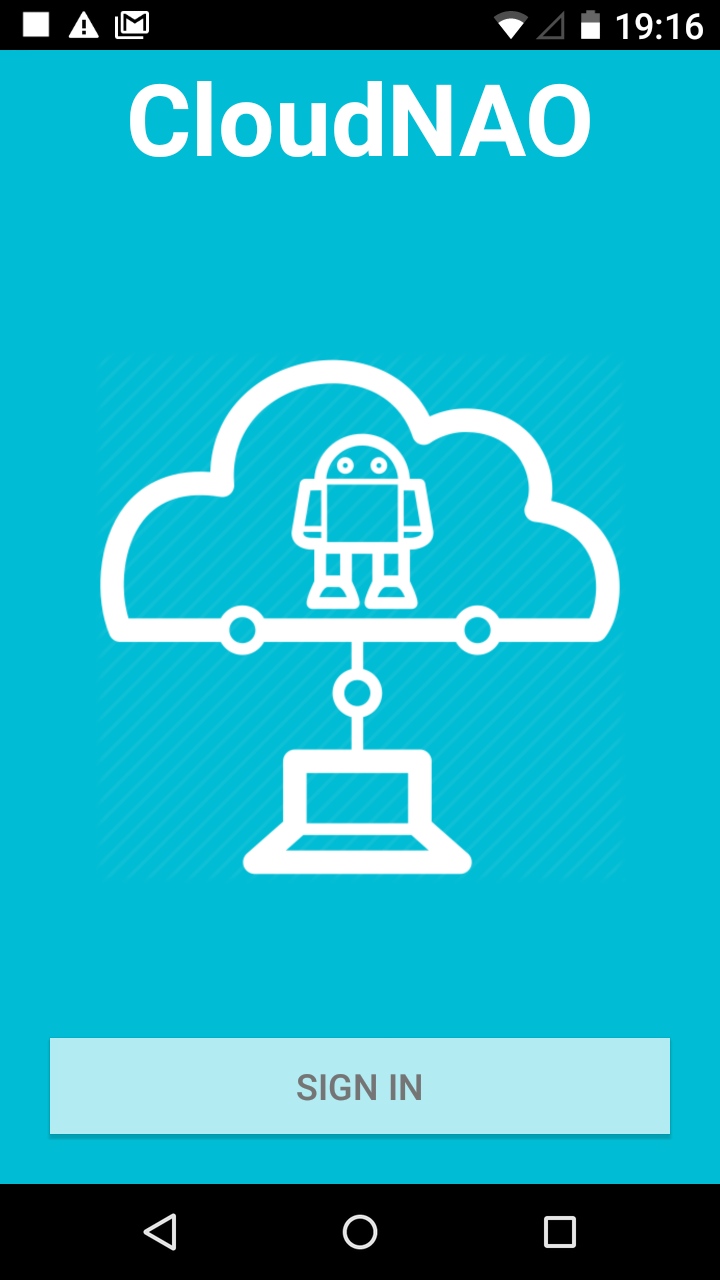
\includegraphics[scale=.1]{signin}}%
    \qquad
    \subfloat{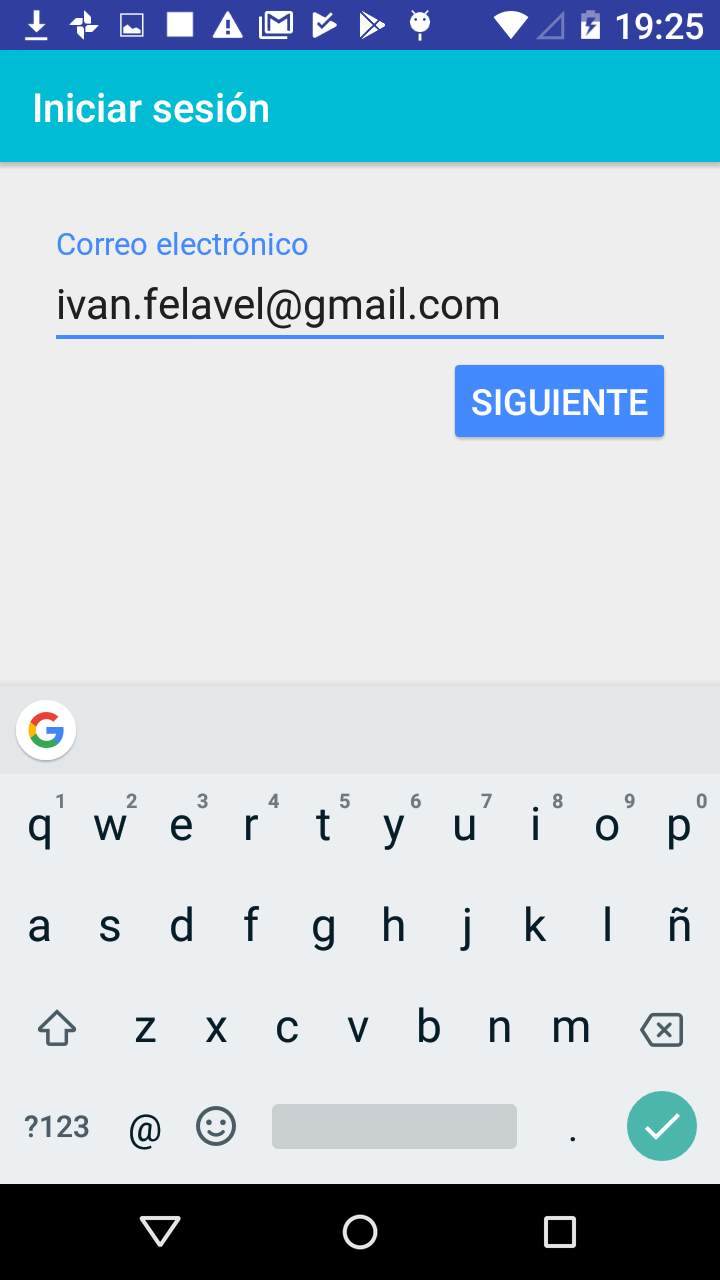
\includegraphics[scale=.1]{signin1}}%
    \qquad
    \subfloat{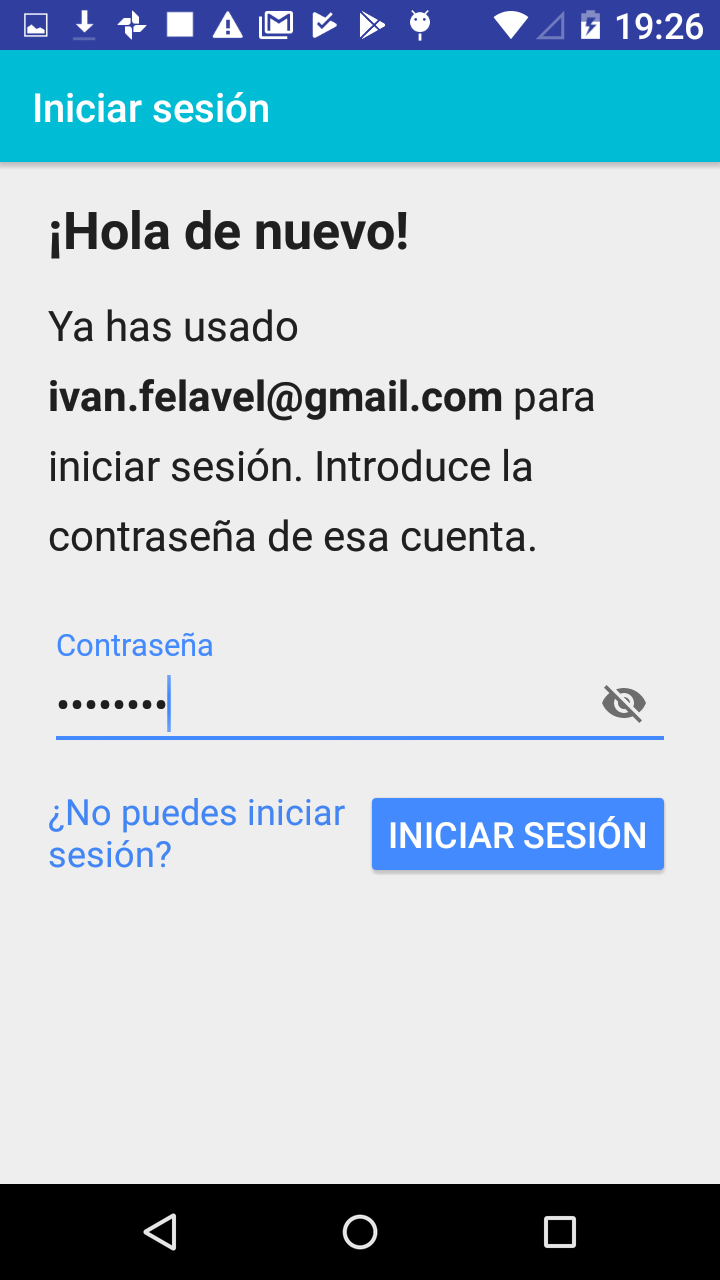
\includegraphics[scale=.1]{signin2}}%
\end{figure}

\subparagraph{Selección y adición de robots a la aplicación.}
\label{\detokenize{users_docs:los-usuarios-pueden-anadir-nuevos-robots}}
Para llevar un control de los robots que tiene un usuario se le permite añadir
los robots que sean necesarios.
Además el usuario cuenta con una lista que le muestra los robots disponibles
que previamente creó.

\begin{figure}[!ht]
    \centering
    \subfloat{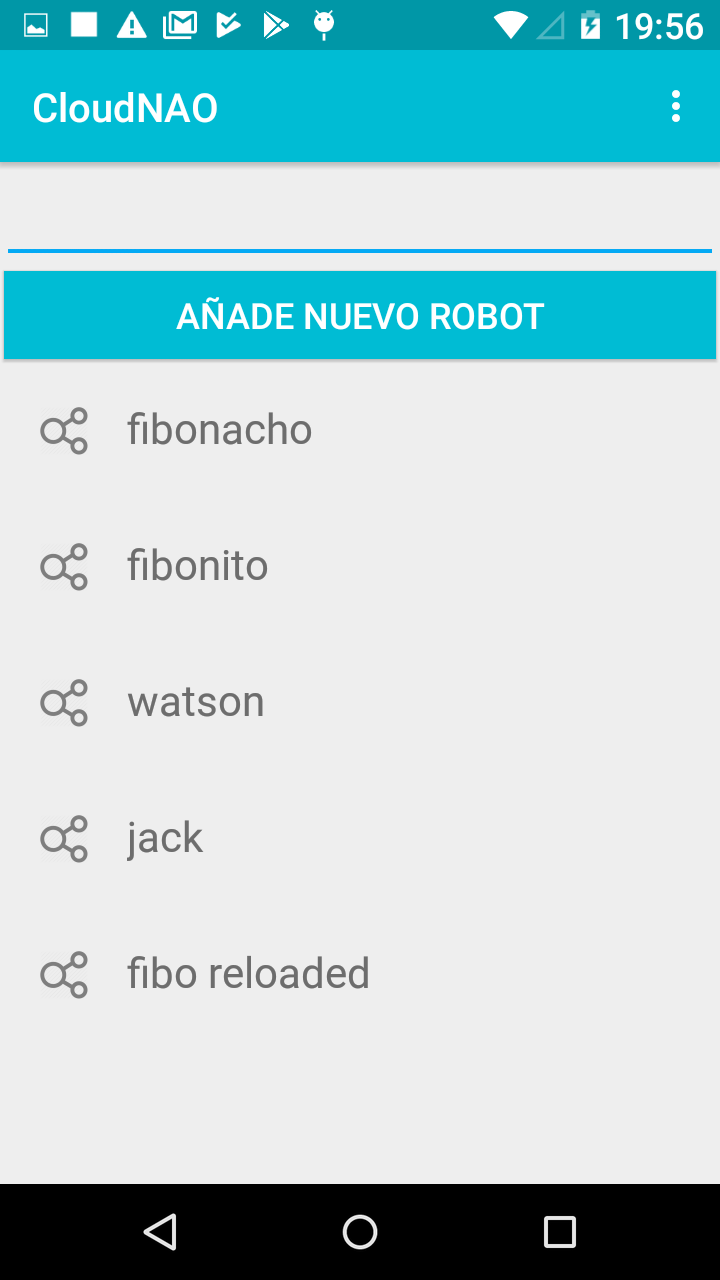
\includegraphics[scale=.1]{add_robot1}}%
    \qquad
    \subfloat{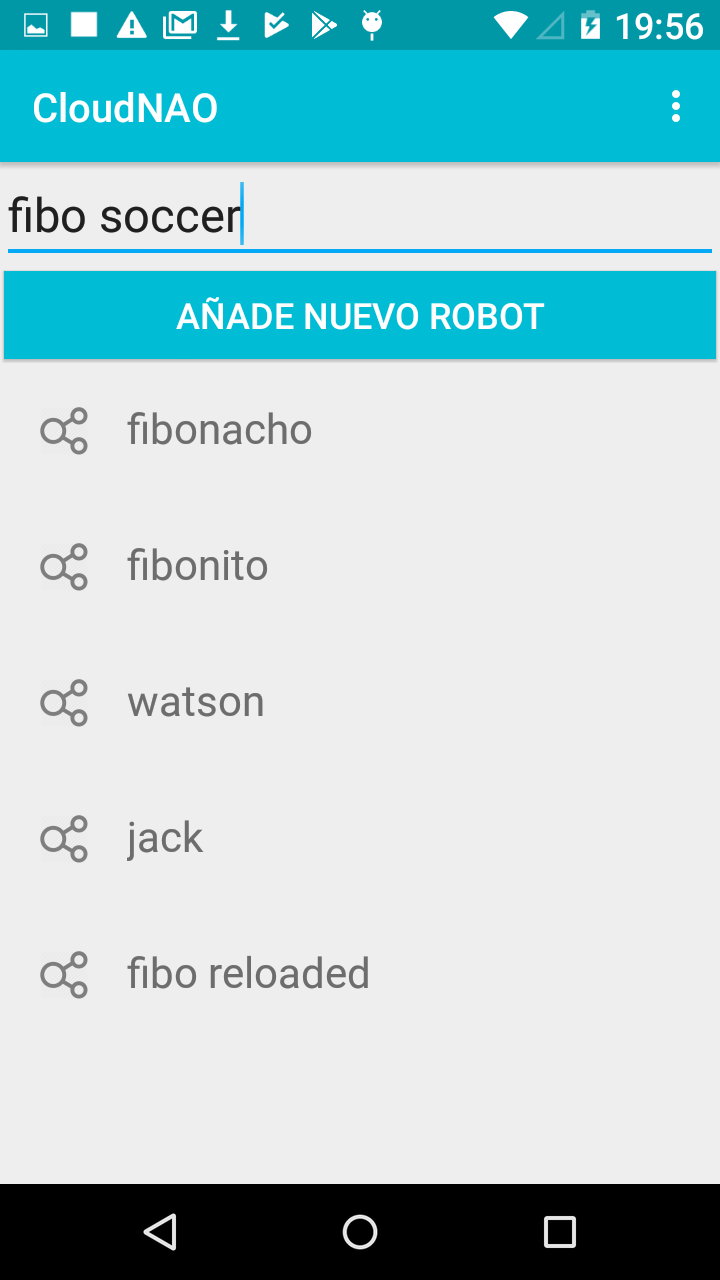
\includegraphics[scale=.1]{add_robot2}}%
    \qquad
    \subfloat{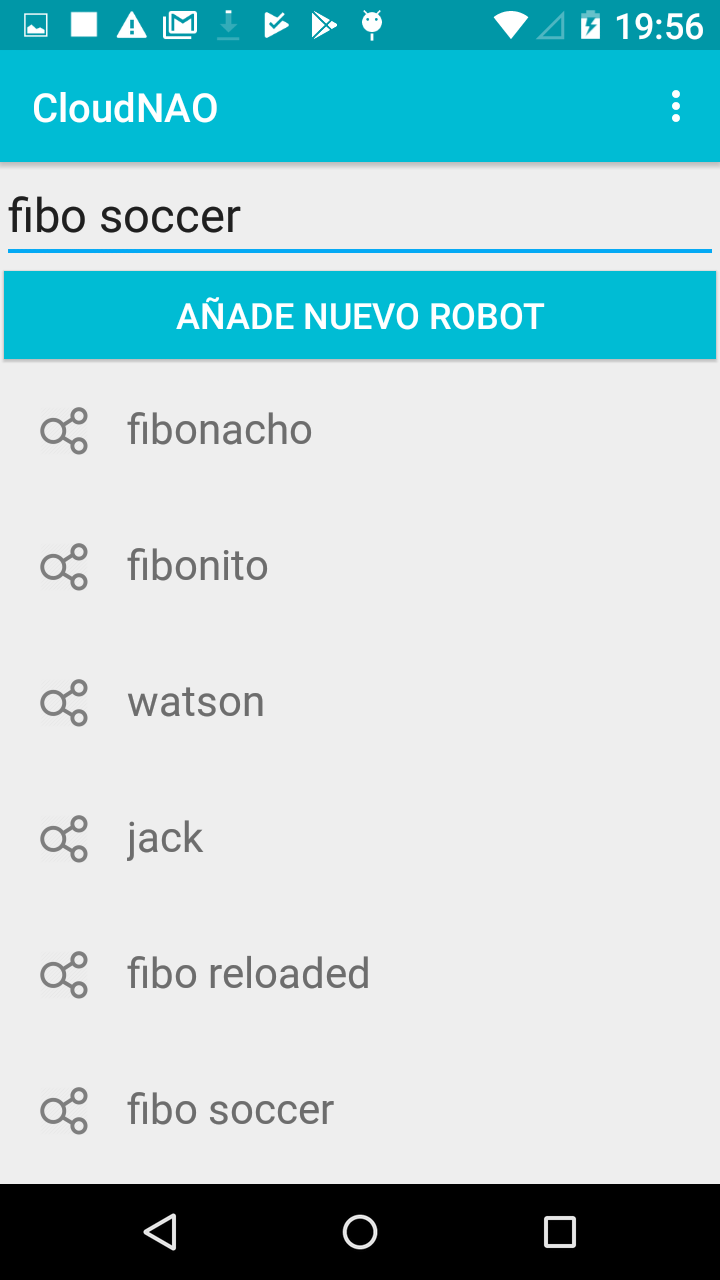
\includegraphics[scale=.1]{add_robot3}}%
    \caption{La aplicación se conecta con Firebase para obtener los
    robot creados y al crear uno se añade a la Firebase Realtime Database.}
    
\end{figure}



\subparagraph{Conexión con un robot seleccionado.}
\label{\detokenize{users_docs:conexion-con-un-robot-seleccionado}}
Al elegir un robot entre los que el usuario posee, simplemente escribe la
dirección IP del robot, y se crea una conexión con éste dentro de la misma
red. Con esto, es posible acceder a todas las características disponibles en la
aplicación.


\begin{figure}[!ht]
    \centering
    \subfloat{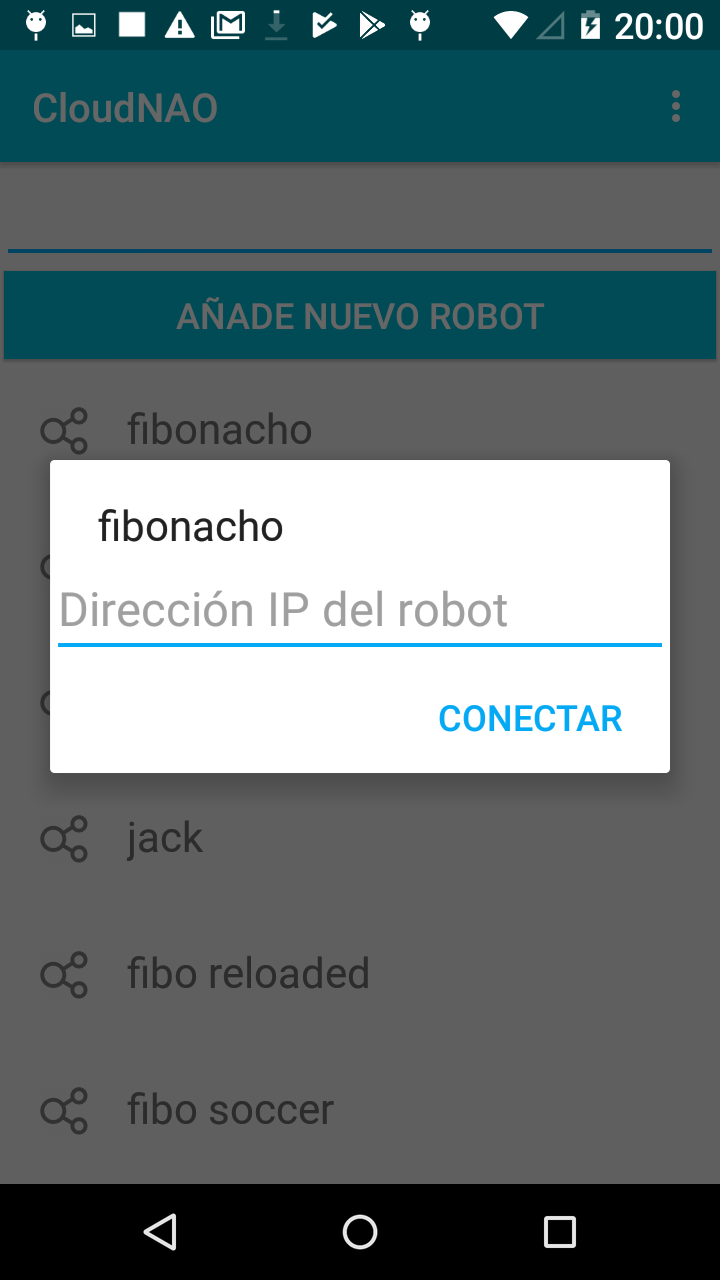
\includegraphics[scale=.1]{robot_connection_app1}}%
    \qquad
    \subfloat{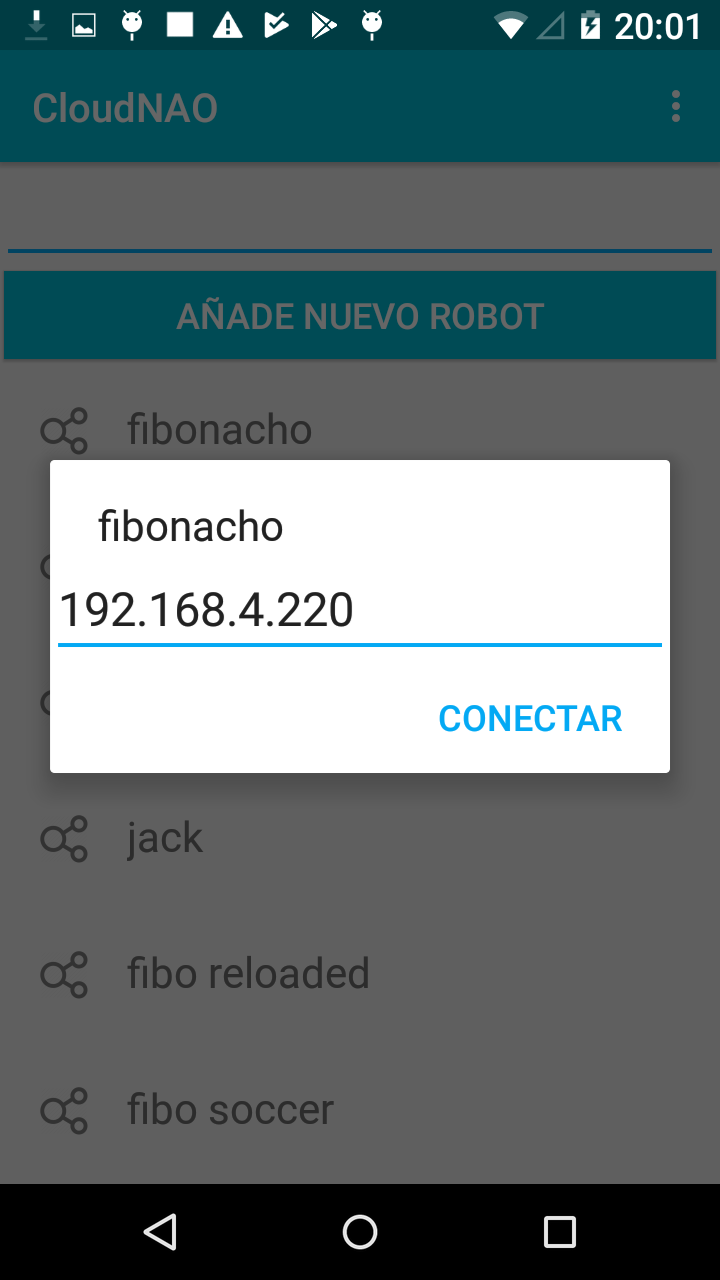
\includegraphics[scale=.1]{robot_connection_app2}}%
    \caption{Para conectarse con un robot simplemente se ingresa la dirección
    IP de éste.}
    
\end{figure}


\subparagraph{Menú intuitivo.}
Las actividades que se pueden realizar después de conectar
la aplicación con el robot se muestran en un menú intuitivo.

\begin{figure}[!ht]
    \centering

    \subfloat{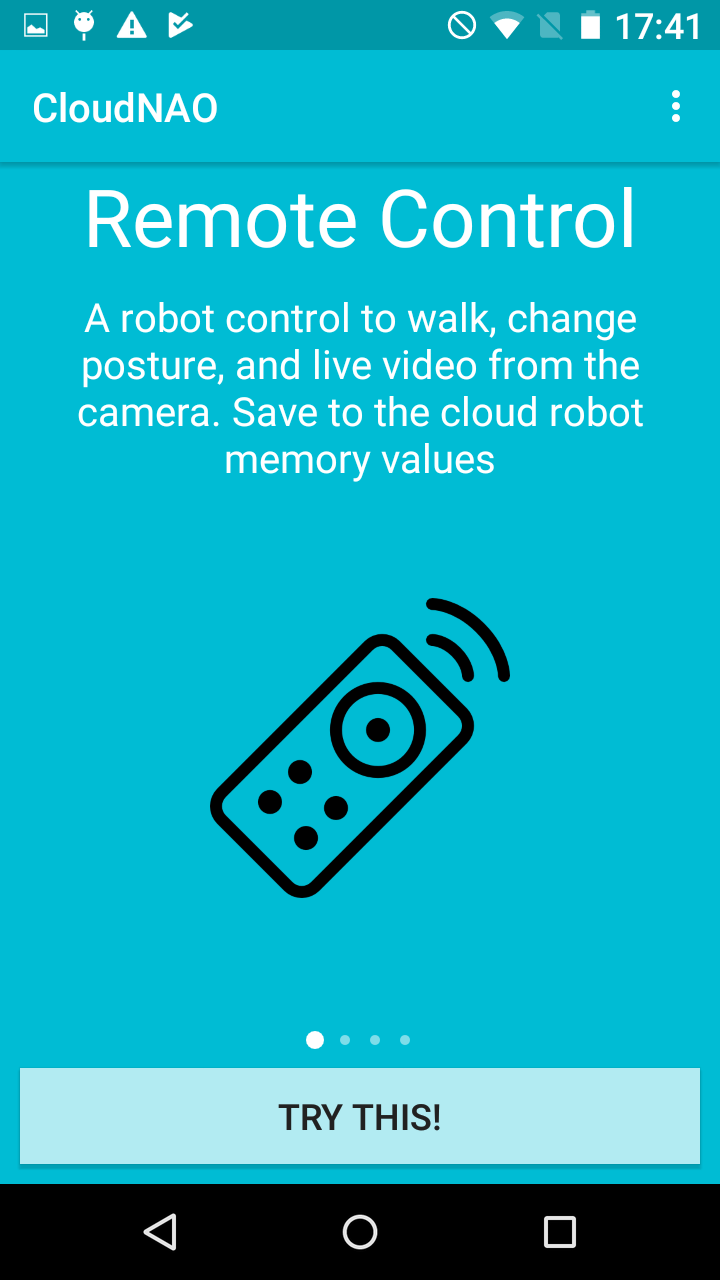
\includegraphics[scale=.09]{menu_rc}}%
    \qquad
    \subfloat{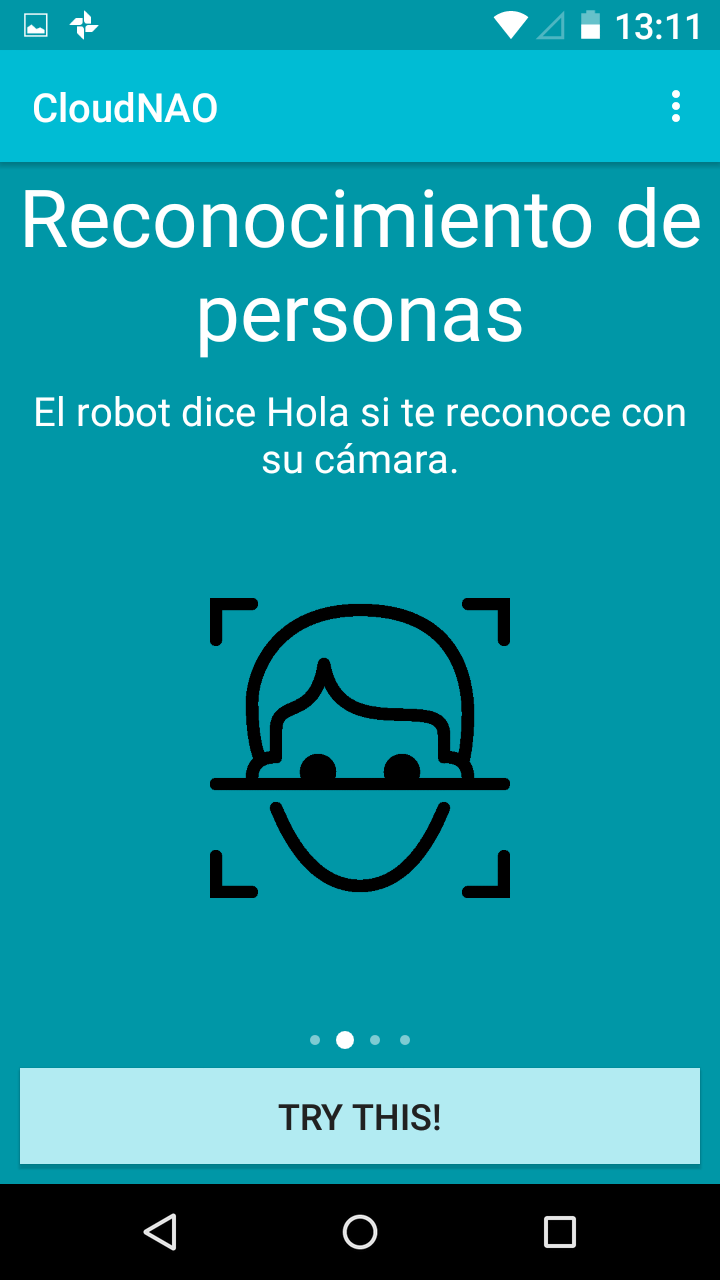
\includegraphics[scale=.09]{menu_face}}%
    \qquad
    \subfloat{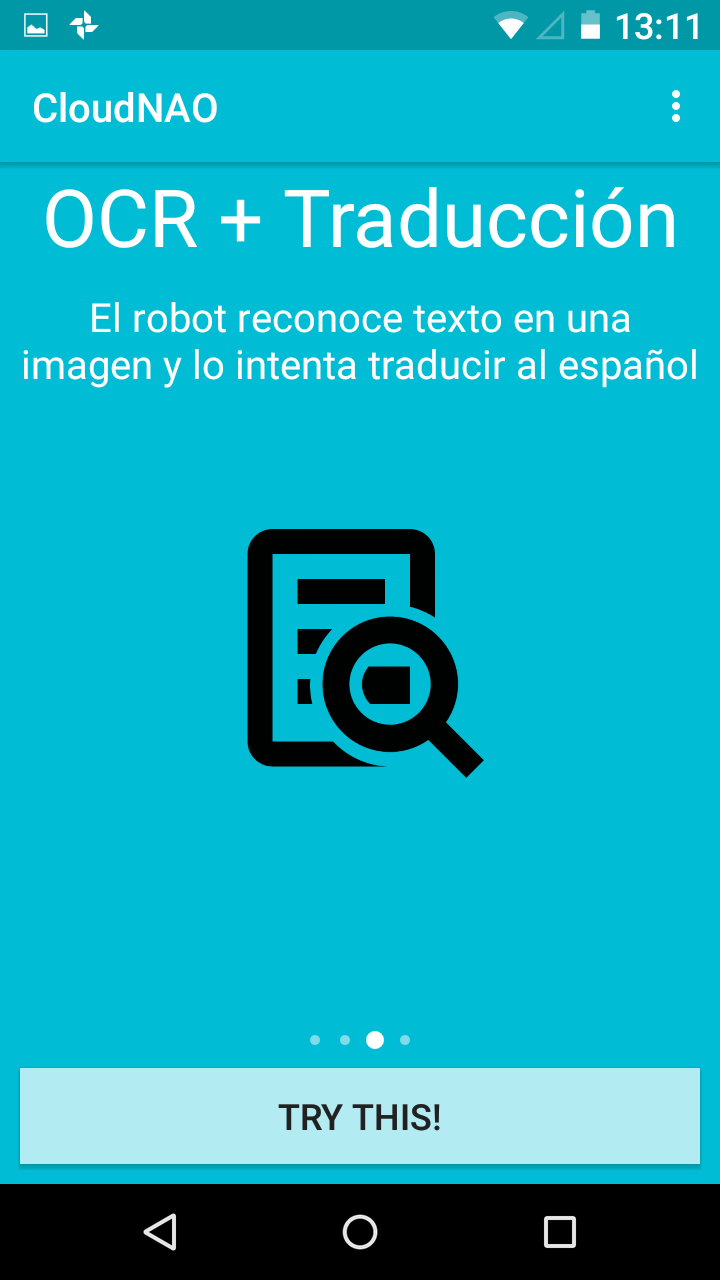
\includegraphics[scale=.09]{menu_ocr}}%
    \qquad
    \subfloat{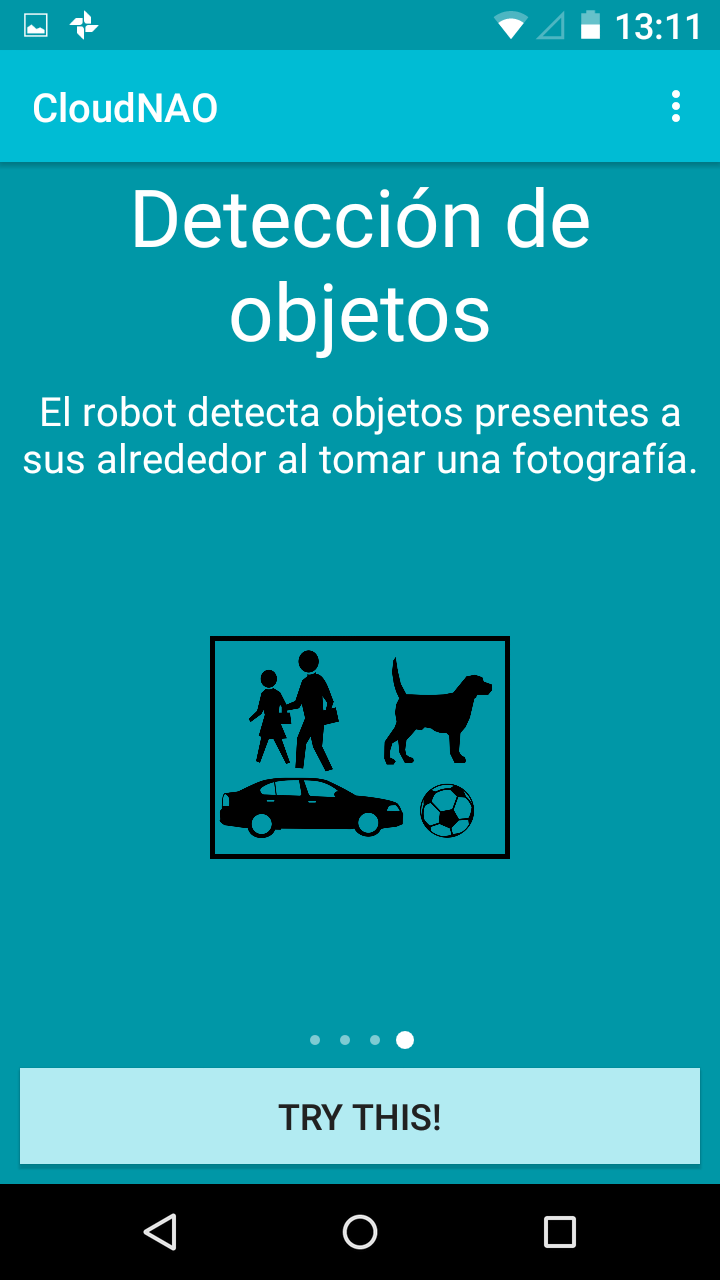
\includegraphics[scale=.09]{menu_objects}}%
    \caption{La pantallas del menú de la aplicación.}
\end{figure}



\subparagraph{Control remoto.}
\label{\detokenize{users_docs:control-remoto-para-el-robot}}
Una primera necesidad que se encontró y por la que surgió todo el proyecto
fue crear un control remoto para el robot NAO. Es muy básico pero admite
comandos para hacer al robot caminar sobre sus tres ejes y cambiar entre dos
posturas. El control remoto incluye una imagen en vivo de la
cámara del robot.

\begin{figure}[!ht]
    \centering
	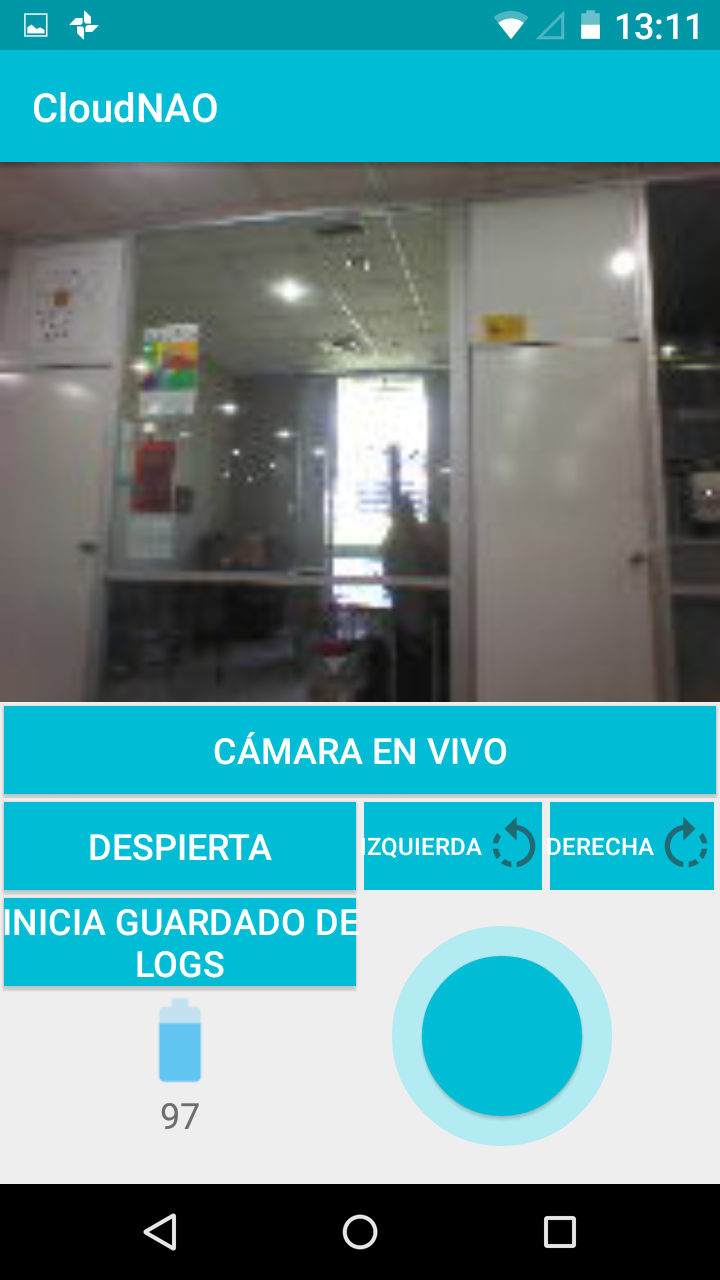
\includegraphics[scale=.1]{rc_image}
	\caption{El control remoto muestra una imagen en vivo si se desea, el estado del batería y un joystick para mover al robot.}
\end{figure}


\subparagraph{Guarda valores de ALMemory en la nube.}
\label{\detokenize{users_docs:guarda-valores-de-almemory-en-la-nube}}
Otra función dentro del control remoto es la de la opción de guardar ciertos
valores de la memoria del robot en la nube, para consultarlos o descargarlos
después en la aplicación web. El conjunto de valores que por ahora
están disponibles para su almacenamiento son los siguientes:
rightUSSensorValue, leftUSSensorValue, rightFootTotalWeight, RightBumperPressed, leftFootTotalWeight, ChestButtonPressed, RearTactilTouched, leftFootContact, LeftBumperPressed, footContact, FrontTactilTouched, BatteryChargeChanged, PostureChanged, rightFootContact, MiddleTactilTouched, GyrometerX, GyrometerY, AccelerometerX, AccelerometerY, AccelerometerZ, TorsoAngleX y TorsoAngleY.

\begin{figure}[!ht]
    \centering
    \subfloat{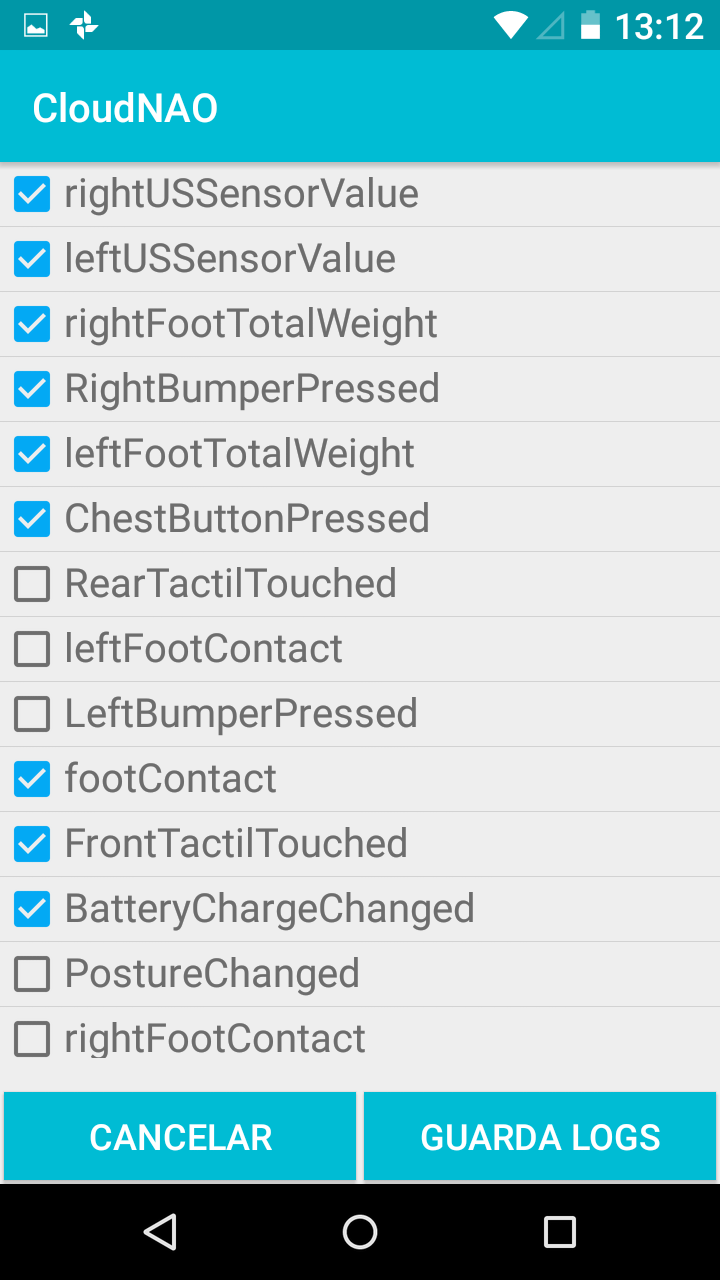
\includegraphics[scale=.1]{memory_list}}%
    \qquad
    \subfloat{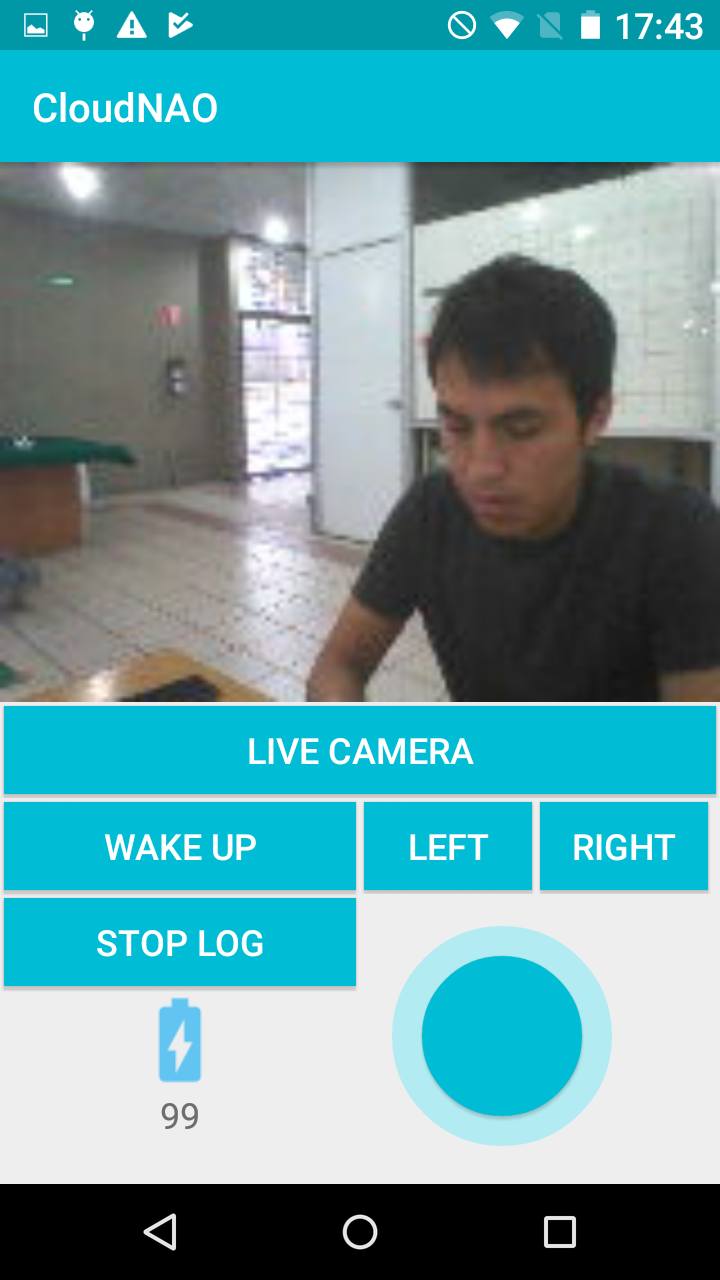
\includegraphics[scale=.1]{rc_image3}}
    \caption{Después de dar clic en el botón INICIA GUARDADO DE LOGS se abre una pantalla para elegir los valores de la memoria que se desean guardar
    en Firebase.}
\end{figure}


\subparagraph{Detección de rostros y reconocimiento de sujetos en una fotografía enviada por el robot.}
\label{\detokenize{users_docs:deteccion-de-rostros-en-una-fotografia-enviada-por-el-robot}}
Esta funcionalidad permite a un usuario
capturar una fotografía con la cámara del robot, añadir
una etiqueta a un rostro si fue encontrado y guardar esa cara para su futuro reconocimiento.
Cuando detecta a un sujeto previamente guardado el robot ejecuta 
un gesto de saludo.

\begin{figure}[!ht]
    \centering
    
    \subfloat{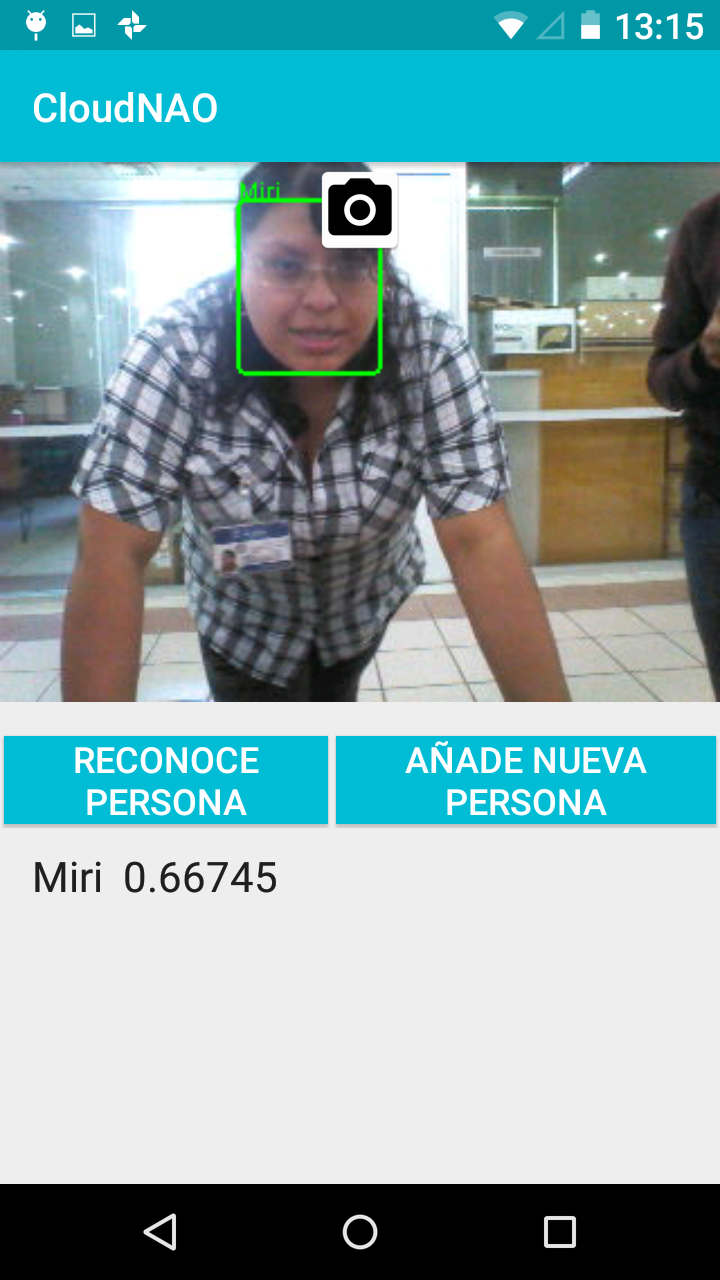
\includegraphics[scale=.1]{face}}%
\caption{Ejemplo de el reconocimiento de una persona que antes fue detectada.}
\end{figure}


\subparagraph{Detección de objetos de entre 80 categorías en una imagen de la cámara del robot.}
\label{\detokenize{users_docs:deteccion-de-objectos-de-entre-80-categorias-en-una-imagen-de-la-camara-del-robot}}
Funciona de manera similar a la detección de rostros. Envía una imagen capturada
con la cámara del robot a la API REST, que ejecuta un módulo
con la API de detección de objetos de TensorFlow y se procesa la respuesta para
que en la pantalla se dibujen unos
recuadros delimitadores sobre los objetos detectados así como una etiqueta
con el nombre que le corresponde. El robot simplemente
dice la cantidad de objetos que ve de acuerdo a las categorías válidas.

\begin{figure}[htbp]
    \centering
	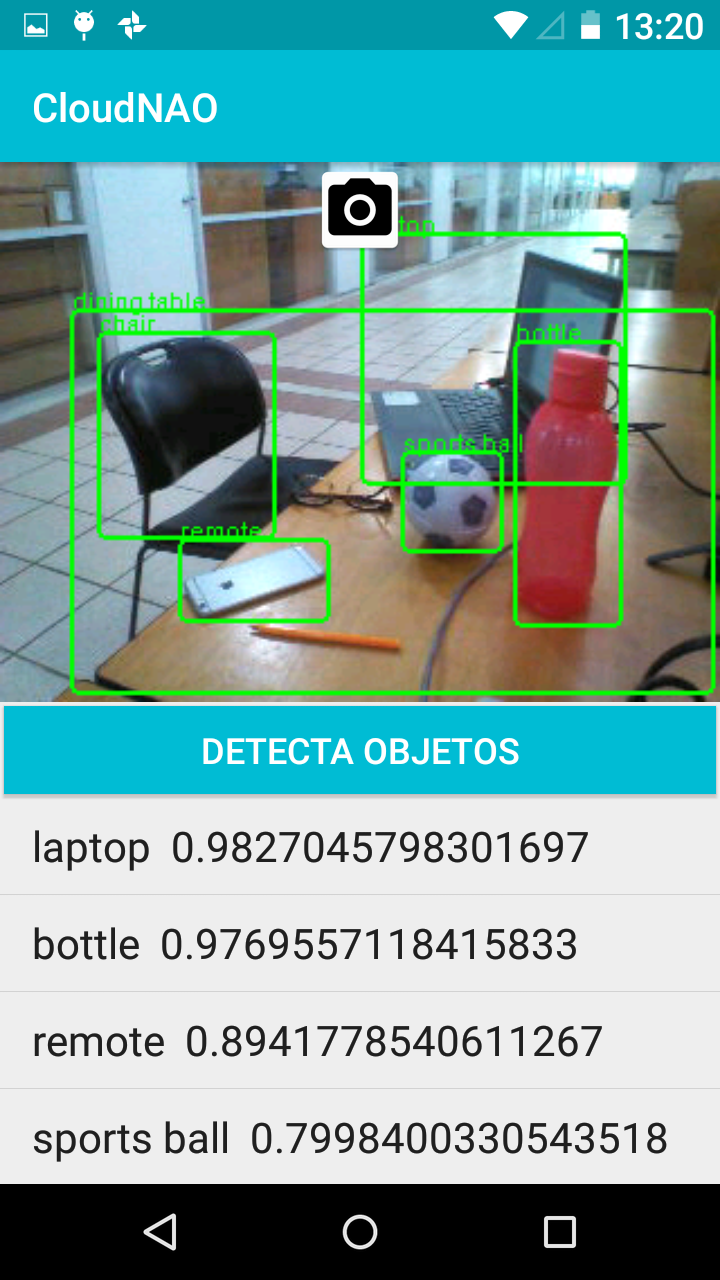
\includegraphics[scale=.1]{object}%
	\caption{Después de detectar los objetos el robot da una lista enumerada
	de éstos.}
\end{figure}


\subparagraph{Reconocimiento óptico de caracteres y traducción de texto encontrados en una imagen enviada por el robot.}
\label{\detokenize{users_docs:reconocimiento-optico-de-caracteres-y-traduccion-de-texto-encontrados-en-una-imagen-enviada-por-el-robot}}
La aplicación solicita una imagen del robot, esa imagen es parte de la petición
a la API RESTful de CloudNAO, igual que en las dos funcionalidades anteriores.
Se buscan caracteres dentro de la imagen, para su posterior traducción.
El resultado se muestra en dos partes, una es el texto original y el otro
es el texto traducido al español. El robot tiene la opción de convertir la
traducción en un discurso oral.

\begin{figure}[htbp]
    \centering
    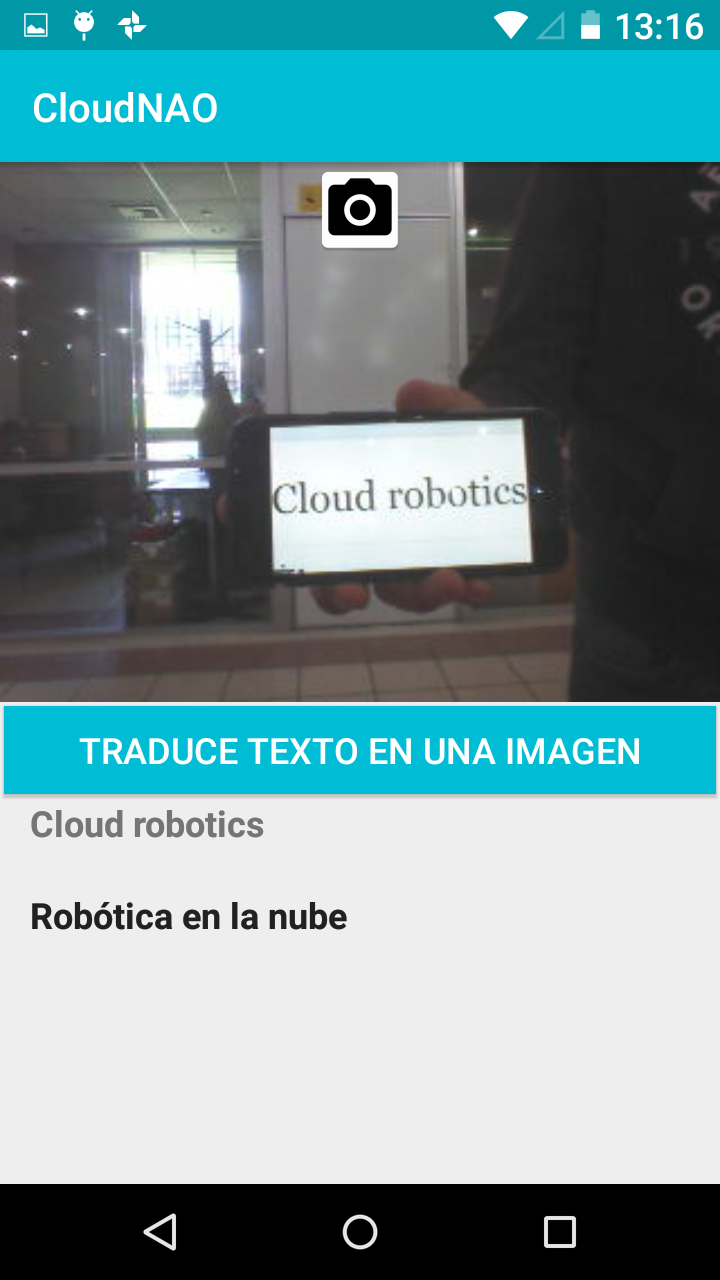
\includegraphics[scale=.1]{ocr_before}
    \caption{Al presionar el texto traducido el robot repite oralmente la cadena
    de caracteres.}
\end{figure}


% \subsubsection{Demostración de la aplicación funcionando}
% \label{\detokenize{users_docs:demostracion-de-la-aplicacion-funcionando}}
% En esta sección se describe de manera pictórica el flujo de la aplicación.
% Desde que el usuario inicia sesión, selecciona un robot y se conecta a él,
% y recorre cada una de las opciones del menú.

% Cada parte va acompañada de una captura de pantalla de la aplicación y
% una fotografía del robot si esta es necesaria.


% \paragraph{Inicio de sesión}
% \label{\detokenize{users_docs:inicio-de-sesion}}

% \paragraph{Selección de Robot}
% \label{\detokenize{users_docs:seleccion-de-robot}}

% \paragraph{Recorrido por el menú}
% \label{\detokenize{users_docs:recorrido-por-el-menu}}

% \paragraph{Control remoto}
% \label{\detokenize{users_docs:control-remoto}}

% \paragraph{Reconocimiento facial}
% \label{\detokenize{users_docs:reconocimiento-facial}}

% \paragraph{Reconocimiento óptico de caracteres y traducción}
% \label{\detokenize{users_docs:reconocimiento-optico-de-caracteres-y-traduccion}}

% \paragraph{Detección de objetos}
% \label{\detokenize{users_docs:deteccion-de-objetos}}

% \paragraph{Cierra la conexión con el robot}
% \label{\detokenize{users_docs:cierra-la-conexion-con-el-robot}}

% \paragraph{Cierra la sesión del usuario}
% \label{\detokenize{users_docs:cierra-la-sesion-del-usuario}}

\subsubsection{Guía para desarrolladores}
\label{\detokenize{dev_docs::doc}}\label{\detokenize{dev_docs:guia-para-desarrolladores}}

Para desarrollar la aplicación fueron tres los elementos importantes:
\begin{itemize}
\item {} 
Un entorno de desarrollo integrado (\textbf{Android Studio}).

\item {} 
El robot humanoide NAO (no simulado).

\item {} 
El SDK para Android de NAOqi.

\end{itemize}

Además de los elementos anteriores se necesitan una computadora y acceso a una red inalámbrica
en cada uno de los dispositivos.
El proyecto se encuentra disponible
a través del repositorio de git
en el siguiente enlace
\url{https://gitlab.com/roboticslab/NAO_Android}.

En el Anexo \ref{anexo:app-android}
se describen las herramientas ocupadas durante 
el desarrollo de la aplicación:
Android Studio, Firebase Realtime
Database, Firebase UI para la autenticación, y las bibliotecas Butterknife
y Volley para el manejo de la IU y para las peticiones a la API REST, respectivamente.




% \subsection{referencias}
% \label{\detokenize{dev_docs:referencias}}
% \sphinxurl{https://developer.android.com/studio/intro/index.html?hl=es-419}
% \sphinxurl{https://medium.com/@petehouston/compile-local-jar-files-with-gradle-a078e5c7a520}
% \sphinxurl{https://github.com/firebase/FirebaseUI-Android/blob/master/auth/README.md}
% \sphinxurl{http://jakewharton.github.io/butterknife/}


\subsubsection{Descripción de las clases principales}
\label{\detokenize{dev_docs:documentacion-para-desarrolladores}}

La aplicación está compuesta como cualquier otra, por una
carpeta \textit{manifests}, \textit{res} y \textit{java}.
La carpeta \textit{java} incluye los paquetes \texttt{com.lar.cloudnao.utilities} y \texttt{com.lar.cloudnao}.


\paragraph{Paquete \texttt{utilities}}

Es un paquete compuesto por clases e interfaces que tienen como
función realizar tareas asíncronas para manejar imágenes del robot,
enviar peticiones a la API REST, manejar la IU, etcétera.\\

\codedocumentation{\texttt{Interface }\sphinxcode{OnRobotNameClickListener}}
Una interfaz con un método abstracto que sirve como callback
cuando un usuario da clic sobre alguno de los robots obtenidos desde Firebase y mostrados en un \texttt{RecyclerView}.
\newline

\codedocumentation{\texttt{Interface }\sphinxcode{VisionRequestCompleted}}
Interfaz con un método abstracto que se llama dentro de una tarea asíncrona para procesar un objeto que se obtiene de la respuesta
a la solicitud del recurso \texttt{vision} de la API REST de CloudNAO.
Hereda métodos de \texttt{AsyncTask}.
\newline

\codedocumentation{\texttt{Class }\sphinxcode{BatteryStatusTask}}
Esta clase obtiene el nivel de batería actual en el robot a través de la lectura del valor en 
\texttt{ALMemory}. Utiliza la clase \texttt{AsyncTask}.
Muestra una \texttt{ImageView} que representa el estado de la batería y un \texttt{TextView} con el porcentaje de batería restante.
\newline

\codedocumentation{\texttt{Class }\sphinxcode{BoundingBoxesUtils}}
Una clase estática con un método para dibujar cuadros delimitadores 
sobre un \texttt{ImageView}. Para dibujar el cuadro delimitador 
recibe un arreglo con los valores necesarios para generar las 
coordenadas que se usan para dibujar.
\newline

\codedocumentation{\texttt{Class }\sphinxcode{ImageTask}}
Clase pública con métodos asíncronos para obtener una imagen desde la cámara del robot de manera remota.  Obtiene un objeto que contiene la imagen, con el espacio de color por defecto del robot NAO (YUV) en un arreglo de bytes, convierte ese arreglo en una imagen jpeg, para después cargar ese objeto jpeg en un bitmap que sirve para llenar el \texttt{ImageView} que muestra la imagen enviada por el robot. Es una subclase
de \texttt{AsyncTask}.
\newline

\codedocumentation{\texttt{Class }\sphinxcode{ItemsListAdapter}}
Esta clase es el \texttt{Adapter} para el \texttt{ListView} cuyos elementos 
están compuestos por un \texttt{CheckBox} y un \texttt{TextView}. Se 
utiliza al mostrar la lista de datos que se quieren guardar en 
Firebase desde \texttt{ALMemory}.
\newline

\codedocumentation{\texttt{Class }\sphinxcode{MyPagerAdapter}}
Subclase de \texttt{PagerAdapter} para el \texttt{ViewPager} del menú
principal de la aplicación, por ahora tiene un tamaño máximo de 4. 
\newline

\codedocumentation{\texttt{Class }\sphinxcode{ProxySubscriberItem}}
Clase pública para modelar los objetos de la lista con los datos de \texttt{ALMemory} que se guardarán en Firebase. \texttt{ItemsListAdapter} contiene un objeto \texttt{List} de
instancias de \texttt{ProxySubscriberItem}. Los
atributos son un  valor booleano \texttt{mChecked} y una cadena \texttt{mProxyName} para saber si un ítem está marcado y el nombre
de la llave en \texttt{ALMemory}, respectivamente.
\newline

\codedocumentation{\texttt{Class }\sphinxcode{RecyclerViewAdapter}}
La clase pública del \texttt{Adapter} para el \texttt{RecyclerView} que mostrará la lista de robots obtenidos desde Firebase y que le pertenecen al
usuario que inició sesión en la aplicación.
\newline

\codedocumentation{\texttt{Class }\sphinxcode{RecyclerViewHolders}}
La clase que modela a los \texttt{ViewHolders} que representan cada robot obtenido de Firebase.
Aquí se utiliza el método abstracto \texttt{onClickRobotName} como callback para ejecutar una acción al dar clic sobre un elemento del \texttt{RecyclerView}.
\newline

\codedocumentation{\texttt{Class }\sphinxcode{RobotFromFirebase}}
La clase que modela los objetos de la lista de robots obtenidos desde Firebase, cada objeto contiene un identificador único y el nombre que el usuario asignó.
\newline

\codedocumentation{\texttt{Class }\sphinxcode{RobotLogs}}
Clase con métodos asíncronos para almacenar valores de \texttt{ALMemory} en Firebase, obtiene valores del robot y los almacena en una ubicación en Firebase con un \texttt{push()}, por lo que se genera un historial de logs.
\newline

\codedocumentation{\texttt{Class }\sphinxcode{ViewHolder}}
Clase que modela los \texttt{ViewHolders} de la lista de datos que se desean guardar en Firebase, están compuestos por un \texttt{CheckBox} y un \texttt{TextView} que describe a cada elemento.
\newline

\codedocumentation{\texttt{Class }\sphinxcode{VisionListElement}}
Clase pública que modela los objetos dentro de una lista que muestra resultados de las actividades de reconocimiento de rostros y objetos. Cada instancia tiene un identificador, que puede ser el nombre del sujeto reconocido , la confianza y las coordenadas de que delimitan al elemento encontrado (un cuadro que encierra un rostro, o un rectángulo que acota un objeto).
\newline

\codedocumentation{\texttt{Class }\sphinxcode{VisionRESTRequestsTask}}
La clase con métodos asíncronos para hacer peticiones a la API REST 
de CloudNAO. Recibe la imagen desde un \texttt{ImageView}, del que obtiene un 
bitmap y genera una cadena en base 64 que representa esa imagen. 
Después define la estructura y valores del JSON que se envía en una 
petición usando la biblioteca Volley. A partir de la respuesta 
obtenida ejecuta la función callback \texttt{onVisionRequestCompleted} 
para mostrar los resultados en el contexto de donde se solicitó.
\newline

\codedocumentation{\texttt{Class }\sphinxcode{VolleyResponseUtils}}
Clase estática para manejar la repuesta de \texttt{Volley}, que puede ser un error o puede ser la estructura que se espera.
\newline

\codedocumentation{\texttt{Enum ModelObjectViewPager}}
Un enumerado de Java que representa todas las posibles páginas del \texttt{ViewPager}. Se utiliza en el menú de la aplicación. En este enumerado se almacenan el identificador del \texttt{Layout} de cada página y un título que le corresponde.


\paragraph{Actividades de la aplicación}

\codedocumentation{\texttt{Class FaceRecognitionActivity}}
La clase de la actividad que realiza el reconocimiento de rostros. Implementa la interfaz \texttt{VisionRequestCompleted} para llamar a su método abstracto desde la clase \texttt{VisionRESTRequestsTask}.
\newline

\codedocumentation{\texttt{Class MenuActivity}}
La actividad que muestra el menú principal donde se elige entre otras actividades para interactuar con el robot. Muestra un \texttt{ViewPager} para navegar y elegir la actividad deseada.
\newline

\codedocumentation{\texttt{Class ObjectDetectionActivity}}
La actividad encargada de la funcionalidad de la detección de objetos, implementa la interfaz \texttt{VisionRequestCompleted} para ejecutar su método \texttt{onVisionRequest\\Completed(Object)} como callback en \texttt{VisionRESTRequestsTask}.
\newline

\codedocumentation{\texttt{Class OCRTranslationActivity}}
Clase de la actividad que se encarga del procesamiento de una imagen 
para detección de texto y su traducción. Implementa la interfaz 
\texttt{VisionRequestCompleted}.
\newline

\codedocumentation{\texttt{Class RemoteControllerActivity}}
La actividad para el control remoto del robot. Además de poder 
controlar algunos movimientos como el caminado o el cambio de postura, 
se puede visualizar una imagen en vivo de la cámara del robot, así 
como permite enviar valores de \texttt{ALMemory} a una base de datos en la nube 
a través de Firebase.
\newline

\codedocumentation{\texttt{Class Robot}}
No es una actividad pero es la clase pública principal para ejecutar módulos del framework de NAOqi en la aplicación. Es una interfaz para conectarse al robot y ejecutar algunos módulos de NAOqi. Usa el patrón de diseño Singleton para que solo exista una instancia del objeto y funcione como una variable global.
\newline

\codedocumentation{\texttt{Class SelectRobotActivity}}
Actividad que muestra los robots registrados por el usuario así como la opción para añadir nuevos robots, o conectarse a uno de la lista. Implementa el método abstracto \texttt{OnRobotNameClickListener.onClickRobotName(String, String)}.

%
%\begin{itemize}
%\item {} 
%\sphinxcode{SignInActivity}, la actividad encargada de todo el flujo para el inicio de sesión. Utiliza FirebaseUI.
%
%\item {} 
%\sphinxcode{SelectRobotActivity}, la actividad que muestra los robots guardados por el usuario que inició sesión. Además aquí se pueden añadir nuevos. Escribe y lee de Firebase Realtime Database. Aquí se crea la instancia única del robot con el que se desea conectar, se crea la sesión y los proxies a los módulos de NAOqi.
%
%\item {} 
%\sphinxcode{MenuActivity}, esta actividad es un menú para elegir entre las actividades restantes. Es un ViewPager, que reacciona al click del usuario.
%
%\item {} 
%\sphinxcode{RemoteControllerActivity}, la actividad que corresponde al control remoto. Utiliza módulos de NAOqi, y la base de datos de Firebase para escribir los logs.
%
%\item {} 
%\sphinxcode{FaceRecognitionActivity}, la actividad que detecta rostros en una imagen. Utiliza Volley para conectarse a la API RESTful de CloudNAO.
%
%\item {} 
%\sphinxcode{OCRTranslationActivity}, esta actividad reconoce texto en una imagen y lo traduce. Utiliza Volley para conectarse a la API RESTful de CloudNAO.
%
%\item {} 
%\sphinxcode{ObjectDetectionActivity}, la actividad que reconoce objetos en una imagen. Utiliza Volley para conectarse a la API RESTful de CloudNAO.
%
%\item {} 
%\sphinxcode{Robot}, es la clase que define al objeto robot. Los métodos para ejecutar módulos de NAOqi, y obtener imágenes de la cámara del robot, valores de la memoria, etc.
%
%\end{itemize}


% \textbf{SignInActivity}
% \label{\detokenize{dev_docs:signinactivity}}\index{SignInActivity (Java class)}

% \begin{fulllineitems}
% \phantomsection\label{\detokenize{dev_docs:com.lar.cloudnao.SignInActivity}}\pysigline{public class \sphinxbfcode{SignInActivity} extends AppCompatActivity}
% La actividad para iniciar sesión en la aplicación, utiliza la biblioteca Firebae UI, para facilitar el flujo del inicio de sesión.

% \end{fulllineitems}



% \textbf{Métodos}
% \label{\detokenize{dev_docs:methods}}

% \textbf{OnClickSignInButton}
% \label{\detokenize{dev_docs:onclicksigninbutton}}\index{OnClickSignInButton() (Java method)}

% \begin{fulllineitems}
% \phantomsection\label{\detokenize{dev_docs:com.lar.cloudnao.SignInActivity.OnClickSignInButton()}}\pysiglinewithargsret{public void \sphinxbfcode{OnClickSignInButton}}{}{}
% Agrega un escuchador al botón signInButton para crear un intent sign-in. Este intent es provisto por la biblioteca de Firebase AuthUI. Esto construye una actividad sign-in, y pasa un entero RC\_SIGN\_IN, que es una variable donde se guarda la respuesta de la actividad sign-in. Cuando esa actividad finaliza su trabajo enviará de regreso onActivityResult que contiene el código de petición y otra información. Esa información es un intent, que podemos usar para descifrar que pasó.

% \end{fulllineitems}



% \textbf{createIntent}
% \label{\detokenize{dev_docs:createintent}}\index{createIntent(Context) (Java method)}

% \begin{fulllineitems}
% \phantomsection\label{\detokenize{dev_docs:com.lar.cloudnao.SignInActivity.createIntent(Context)}}\pysiglinewithargsret{public static Intent \sphinxbfcode{createIntent}}{Context\sphinxstyleemphasis{ context}}{}
% Este método se utiliza por la actividad sign-in en caso de que no se tenga un usuario válido.

% \end{fulllineitems}



% \textbf{onActivityResult}
% \label{\detokenize{dev_docs:onactivityresult}}\index{onActivityResult(int, int, Intent) (Java method)}

% \begin{fulllineitems}
% \phantomsection\label{\detokenize{dev_docs:com.lar.cloudnao.SignInActivity.onActivityResult(int, int, Intent)}}\pysiglinewithargsret{protected void \sphinxbfcode{onActivityResult}}{int\sphinxstyleemphasis{ requestCode}, int\sphinxstyleemphasis{ resultCode}, Intent\sphinxstyleemphasis{ data}}{}
% Verifica y maneja el resultado enviado por la actividad sign-in

% \end{fulllineitems}



% \textbf{onCreate}
% \label{\detokenize{dev_docs:oncreate}}\index{onCreate(Bundle) (Java method)}

% \begin{fulllineitems}
% \phantomsection\label{\detokenize{dev_docs:com.lar.cloudnao.SignInActivity.onCreate(Bundle)}}\pysiglinewithargsret{protected void \sphinxbfcode{onCreate}}{Bundle\sphinxstyleemphasis{ savedInstanceState}}{}
% Es el método que se llama al crear la actividad, si el usuario ya ha iniciado sesión ejecuta la actividad de la clase SelectRobotActivity y finaliza la actual.

% \end{fulllineitems}



% \textbf{SelectRobotActivity}
% \label{\detokenize{dev_docs:selectrobotactivity}}\index{SelectRobotActivity (Java class)}

% \begin{fulllineitems}
% \phantomsection\label{\detokenize{dev_docs:com.lar.cloudnao.SelectRobotActivity}}\pysigline{public class \sphinxbfcode{SelectRobotActivity} extends AppCompatActivity implements OnRobotNameClickListener}
% Actividad que muestra los robots registrados por el usuario así como la opción para añadir nuevos robots, o conectarse a uno de la lista. Implementa el método abstracto \sphinxcode{OnRobotNameClickListeneronClickRobotName(String,String)}.

% \end{fulllineitems}



% \subsubsection{Atributos}
% \label{\detokenize{dev_docs:fields}}

% \paragraph{MyRobot}
% \label{\detokenize{dev_docs:myrobot}}\index{MyRobot (Java field)}

% \begin{fulllineitems}
% \phantomsection\label{\detokenize{dev_docs:com.lar.cloudnao.SelectRobotActivity.MyRobot}}\pysigline{public {\hyperref[\detokenize{dev_docs:com.lar.cloudnao.Robot}]{\sphinxcrossref{Robot}}} \sphinxbfcode{MyRobot}}
% Llama a las instancia global de {\hyperref[\detokenize{dev_docs:com.lar.cloudnao.Robot}]{\sphinxcrossref{\sphinxcode{Robot}}}}

% \end{fulllineitems}



% \paragraph{mNewRobotEditText}
% \label{\detokenize{dev_docs:mnewrobotedittext}}\index{mNewRobotEditText (Java field)}

% \begin{fulllineitems}
% \phantomsection\label{\detokenize{dev_docs:com.lar.cloudnao.SelectRobotActivity.mNewRobotEditText}}\pysigline{ EditText \sphinxbfcode{mNewRobotEditText}}
% Campo para añadir el nombre de un nuevo robot.

% \end{fulllineitems}



% \paragraph{robotListFromFirebaseRecyclerView}
% \label{\detokenize{dev_docs:robotlistfromfirebaserecyclerview}}\index{robotListFromFirebaseRecyclerView (Java field)}

% \begin{fulllineitems}
% \phantomsection\label{\detokenize{dev_docs:com.lar.cloudnao.SelectRobotActivity.robotListFromFirebaseRecyclerView}}\pysigline{ RecyclerView \sphinxbfcode{robotListFromFirebaseRecyclerView}}
% La lista de los robots del usuario, se llena desde Firebase.

% \end{fulllineitems}



% \subsubsection{Métodos}
% \label{\detokenize{dev_docs:id3}}

% \paragraph{addNewRobot}
% \label{\detokenize{dev_docs:addnewrobot}}\index{addNewRobot() (Java method)}

% \begin{fulllineitems}
% \phantomsection\label{\detokenize{dev_docs:com.lar.cloudnao.SelectRobotActivity.addNewRobot()}}\pysiglinewithargsret{public void \sphinxbfcode{addNewRobot}}{}{}
% Escuchador para el botón que permite a los usuarios añadir un nuevo robot.

% \end{fulllineitems}



% \paragraph{onClickRobotName}
% \label{\detokenize{dev_docs:onclickrobotname}}\index{onClickRobotName(String, String) (Java method)}

% \begin{fulllineitems}
% \phantomsection\label{\detokenize{dev_docs:com.lar.cloudnao.SelectRobotActivity.onClickRobotName(String, String)}}\pysiglinewithargsret{public void \sphinxbfcode{onClickRobotName}}{\sphinxhref{http://docs.oracle.com/javase/8/docs/api/java/lang/String.html}{String}\sphinxstyleemphasis{ robotName}, \sphinxhref{http://docs.oracle.com/javase/8/docs/api/java/lang/String.html}{String}\sphinxstyleemphasis{ robotUID}}{}
% Define al método abstracto \sphinxcode{OnRobotNameClickListeneronClickRobotName(String,String)} para servir como callback cuando un usuario da clcik en un robot de la lista. Muestra un cuadro de diálogo con TextView para agregar la dirección IP del robot y ejecutar \sphinxcode{ConnectionTask}.

% \end{fulllineitems}



% \paragraph{onCreate}
% \label{\detokenize{dev_docs:id4}}\index{onCreate(Bundle) (Java method)}

% \begin{fulllineitems}
% \phantomsection\label{\detokenize{dev_docs:com.lar.cloudnao.SelectRobotActivity.onCreate(Bundle)}}\pysiglinewithargsret{protected void \sphinxbfcode{onCreate}}{Bundle\sphinxstyleemphasis{ savedInstanceState}}{}
% Inicia la actividad, verifica que el usuario haya iniciado sesión. Si el usuario es nuevo, entonces se añade a la ubicación /users en la base de datos de Firebase. Luego, agrega un escuchador a la ubicación de la base de datos que contiene a los robots del usuario. Llama al método \sphinxcode{getRobotFirebaseDataSnapshot()} para actualizar {\hyperref[\detokenize{dev_docs:com.lar.cloudnao.SelectRobotActivity.robotListFromFirebaseRecyclerView}]{\sphinxcrossref{\sphinxcode{robotListFromFirebaseRecyclerView}}}}.

% \end{fulllineitems}



% \paragraph{onCreateOptionsMenu}
% \label{\detokenize{dev_docs:oncreateoptionsmenu}}\index{onCreateOptionsMenu(Menu) (Java method)}

% \begin{fulllineitems}
% \phantomsection\label{\detokenize{dev_docs:com.lar.cloudnao.SelectRobotActivity.onCreateOptionsMenu(Menu)}}\pysiglinewithargsret{public boolean \sphinxbfcode{onCreateOptionsMenu}}{Menu\sphinxstyleemphasis{ menu}}{}
% Crea un menú de opciones para que por ahora contiene un elemento, cerrar la sesión del usuario.

% \end{fulllineitems}



% \paragraph{onOptionsItemSelected}
% \label{\detokenize{dev_docs:onoptionsitemselected}}\index{onOptionsItemSelected(MenuItem) (Java method)}

% \begin{fulllineitems}
% \phantomsection\label{\detokenize{dev_docs:com.lar.cloudnao.SelectRobotActivity.onOptionsItemSelected(MenuItem)}}\pysiglinewithargsret{public boolean \sphinxbfcode{onOptionsItemSelected}}{MenuItem\sphinxstyleemphasis{ item}}{}
% Añade un escuchador para cuando se selecciona un elemento en el menú de opciones. Por ahora solo cerrar sesión. Llama al método {\hyperref[\detokenize{dev_docs:com.lar.cloudnao.SelectRobotActivity.signOut()}]{\sphinxcrossref{\sphinxcode{signOut()}}}}.

% \end{fulllineitems}



% \paragraph{signOut}
% \label{\detokenize{dev_docs:signout}}\index{signOut() (Java method)}

% \begin{fulllineitems}
% \phantomsection\label{\detokenize{dev_docs:com.lar.cloudnao.SelectRobotActivity.signOut()}}\pysiglinewithargsret{public void \sphinxbfcode{signOut}}{}{}
% Cierra la sesión através de la biblioteca AuthUI

% \end{fulllineitems}



% \textbf{MenuActivity}
% \label{\detokenize{dev_docs:menuactivity}}\index{MenuActivity (Java class)}

% \begin{fulllineitems}
% \phantomsection\label{\detokenize{dev_docs:com.lar.cloudnao.MenuActivity}}\pysigline{public class \sphinxbfcode{MenuActivity} extends AppCompatActivity}
% La actividad que muestra el menú donde se elige entre otras actividades para interactuar con el robot. Muestra un ViewPager para navegar y elegir la actividad deseada.

% \end{fulllineitems}



% \subsubsection{Atributos}
% \label{\detokenize{dev_docs:id5}}

% \paragraph{MyRobot}
% \label{\detokenize{dev_docs:id6}}\index{MyRobot (Java field)}

% \begin{fulllineitems}
% \phantomsection\label{\detokenize{dev_docs:com.lar.cloudnao.MenuActivity.MyRobot}}\pysigline{public {\hyperref[\detokenize{dev_docs:com.lar.cloudnao.Robot}]{\sphinxcrossref{Robot}}} \sphinxbfcode{MyRobot}}
% La instancia del singleton de la clase {\hyperref[\detokenize{dev_docs:com.lar.cloudnao.Robot}]{\sphinxcrossref{\sphinxcode{Robot}}}}

% \end{fulllineitems}



% \paragraph{mCurrentPageSelected}
% \label{\detokenize{dev_docs:mcurrentpageselected}}\index{mCurrentPageSelected (Java field)}

% \begin{fulllineitems}
% \phantomsection\label{\detokenize{dev_docs:com.lar.cloudnao.MenuActivity.mCurrentPageSelected}}\pysigline{public int \sphinxbfcode{mCurrentPageSelected}}
% Un número que identifica la página que se muestra actualmente.

% \end{fulllineitems}



% \subsubsection{Métodos}
% \label{\detokenize{dev_docs:id7}}

% \paragraph{onClickMenuButton}
% \label{\detokenize{dev_docs:onclickmenubutton}}\index{onClickMenuButton() (Java method)}

% \begin{fulllineitems}
% \phantomsection\label{\detokenize{dev_docs:com.lar.cloudnao.MenuActivity.onClickMenuButton()}}\pysiglinewithargsret{public void \sphinxbfcode{onClickMenuButton}}{}{}
% Define el escuchador para el botón de selección de actividad dentro del menú de actividades.

% \end{fulllineitems}



% \paragraph{onCreate}
% \label{\detokenize{dev_docs:id8}}\index{onCreate(Bundle) (Java method)}

% \begin{fulllineitems}
% \phantomsection\label{\detokenize{dev_docs:com.lar.cloudnao.MenuActivity.onCreate(Bundle)}}\pysiglinewithargsret{protected void \sphinxbfcode{onCreate}}{Bundle\sphinxstyleemphasis{ savedInstanceState}}{}
% Inicializa la actividad, el ViewPager y el Adapter para escuchar cuando se cambia de página.

% \end{fulllineitems}



% \paragraph{onCreateOptionsMenu}
% \label{\detokenize{dev_docs:id9}}\index{onCreateOptionsMenu(Menu) (Java method)}

% \begin{fulllineitems}
% \phantomsection\label{\detokenize{dev_docs:com.lar.cloudnao.MenuActivity.onCreateOptionsMenu(Menu)}}\pysiglinewithargsret{public boolean \sphinxbfcode{onCreateOptionsMenu}}{Menu\sphinxstyleemphasis{ menu}}{}
% Crea un menú de opciones, en la barra superior y contar con una opción para desconectarse del robot (cerrando la sesión de NAOqi)

% \end{fulllineitems}



% \paragraph{onOptionsItemSelected}
% \label{\detokenize{dev_docs:id10}}\index{onOptionsItemSelected(MenuItem) (Java method)}

% \begin{fulllineitems}
% \phantomsection\label{\detokenize{dev_docs:com.lar.cloudnao.MenuActivity.onOptionsItemSelected(MenuItem)}}\pysiglinewithargsret{public boolean \sphinxbfcode{onOptionsItemSelected}}{MenuItem\sphinxstyleemphasis{ item}}{}
% Ejecuta la función \sphinxcode{closeRobotConnection()} si se selecciona la opción de desconectarse del robot desde el menú de opciones.

% \end{fulllineitems}



% \paragraph{startOCRActivity}
% \label{\detokenize{dev_docs:startocractivity}}\index{startOCRActivity() (Java method)}

% \begin{fulllineitems}
% \phantomsection\label{\detokenize{dev_docs:com.lar.cloudnao.MenuActivity.startOCRActivity()}}\pysiglinewithargsret{public void \sphinxbfcode{startOCRActivity}}{}{}
% Inicia la actividad {\hyperref[\detokenize{dev_docs:com.lar.cloudnao.OCRTranslationActivity}]{\sphinxcrossref{\sphinxcode{OCRTranslationActivity}}}}

% \end{fulllineitems}



% \paragraph{startObjectDetectionActivity}
% \label{\detokenize{dev_docs:startobjectdetectionactivity}}\index{startObjectDetectionActivity() (Java method)}

% \begin{fulllineitems}
% \phantomsection\label{\detokenize{dev_docs:com.lar.cloudnao.MenuActivity.startObjectDetectionActivity()}}\pysiglinewithargsret{public void \sphinxbfcode{startObjectDetectionActivity}}{}{}
% Inicia la actividad {\hyperref[\detokenize{dev_docs:com.lar.cloudnao.ObjectDetectionActivity}]{\sphinxcrossref{\sphinxcode{ObjectDetectionActivity}}}}

% \end{fulllineitems}



% \textbf{RemoteControllerActivity}
% \label{\detokenize{dev_docs:remotecontrolleractivity}}\index{RemoteControllerActivity (Java class)}

% \begin{fulllineitems}
% \phantomsection\label{\detokenize{dev_docs:com.lar.cloudnao.RemoteControllerActivity}}\pysigline{public class \sphinxbfcode{RemoteControllerActivity} extends AppCompatActivity}
% La actividad para el control remoto del robot. Además de poder controlar algunos movimientos como el caminado o el cambio de postura, se puede visualizar una imagen en vivo de la cámara del robot, así como permite enviar valores de ALMemory a una base de datos en la nube a través de Firebase.

% \end{fulllineitems}



% \subsubsection{Atributos}
% \label{\detokenize{dev_docs:id11}}

% \paragraph{MyRobot}
% \label{\detokenize{dev_docs:id12}}\index{MyRobot (Java field)}

% \begin{fulllineitems}
% \phantomsection\label{\detokenize{dev_docs:com.lar.cloudnao.RemoteControllerActivity.MyRobot}}\pysigline{public {\hyperref[\detokenize{dev_docs:com.lar.cloudnao.Robot}]{\sphinxcrossref{Robot}}} \sphinxbfcode{MyRobot}}
% Llama la instacia global de {\hyperref[\detokenize{dev_docs:com.lar.cloudnao.Robot}]{\sphinxcrossref{\sphinxcode{Robot}}}}

% \end{fulllineitems}



% \paragraph{mBatteryImageView}
% \label{\detokenize{dev_docs:mbatteryimageview}}\index{mBatteryImageView (Java field)}

% \begin{fulllineitems}
% \phantomsection\label{\detokenize{dev_docs:com.lar.cloudnao.RemoteControllerActivity.mBatteryImageView}}\pysigline{ ImageView \sphinxbfcode{mBatteryImageView}}
% Una imagen con el estado de la batería.

% \end{fulllineitems}



% \paragraph{mBatteryTextView}
% \label{\detokenize{dev_docs:mbatterytextview}}\index{mBatteryTextView (Java field)}

% \begin{fulllineitems}
% \phantomsection\label{\detokenize{dev_docs:com.lar.cloudnao.RemoteControllerActivity.mBatteryTextView}}\pysigline{ TextView \sphinxbfcode{mBatteryTextView}}
% El nivel actual de batería del robot.

% \end{fulllineitems}



% \paragraph{mBatteryWaitTimer}
% \label{\detokenize{dev_docs:mbatterywaittimer}}\index{mBatteryWaitTimer (Java field)}

% \begin{fulllineitems}
% \phantomsection\label{\detokenize{dev_docs:com.lar.cloudnao.RemoteControllerActivity.mBatteryWaitTimer}}\pysigline{ \sphinxhref{http://docs.oracle.com/javase/8/docs/api/java/util/Timer.html}{Timer} \sphinxbfcode{mBatteryWaitTimer}}
% El Timer encargado de repetir {\hyperref[\detokenize{dev_docs:com.lar.cloudnao.RemoteControllerActivity.mTimerBatteryStatusTask}]{\sphinxcrossref{\sphinxcode{mTimerBatteryStatusTask}}}}

% \end{fulllineitems}



% \paragraph{mCameraWaitTimer}
% \label{\detokenize{dev_docs:mcamerawaittimer}}\index{mCameraWaitTimer (Java field)}

% \begin{fulllineitems}
% \phantomsection\label{\detokenize{dev_docs:com.lar.cloudnao.RemoteControllerActivity.mCameraWaitTimer}}\pysigline{ \sphinxhref{http://docs.oracle.com/javase/8/docs/api/java/util/Timer.html}{Timer} \sphinxbfcode{mCameraWaitTimer}}
% Un Timer encargado de la ejecución de {\hyperref[\detokenize{dev_docs:com.lar.cloudnao.RemoteControllerActivity.mTimerTaskCamera}]{\sphinxcrossref{\sphinxcode{mTimerTaskCamera}}}}.

% \end{fulllineitems}



% \paragraph{mJoystick}
% \label{\detokenize{dev_docs:mjoystick}}\index{mJoystick (Java field)}

% \begin{fulllineitems}
% \phantomsection\label{\detokenize{dev_docs:com.lar.cloudnao.RemoteControllerActivity.mJoystick}}\pysigline{public Joystick \sphinxbfcode{mJoystick}}
% Instancia del objeto Joystick importado de la biblioteca Bugstick.

% \end{fulllineitems}



% \paragraph{mLiveImageFromRobot}
% \label{\detokenize{dev_docs:mliveimagefromrobot}}\index{mLiveImageFromRobot (Java field)}

% \begin{fulllineitems}
% \phantomsection\label{\detokenize{dev_docs:com.lar.cloudnao.RemoteControllerActivity.mLiveImageFromRobot}}\pysigline{ ImageView \sphinxbfcode{mLiveImageFromRobot}}
% Imagen en vivo del robot.

% \end{fulllineitems}



% \paragraph{mLogsWaitTimer}
% \label{\detokenize{dev_docs:mlogswaittimer}}\index{mLogsWaitTimer (Java field)}

% \begin{fulllineitems}
% \phantomsection\label{\detokenize{dev_docs:com.lar.cloudnao.RemoteControllerActivity.mLogsWaitTimer}}\pysigline{ \sphinxhref{http://docs.oracle.com/javase/8/docs/api/java/util/Timer.html}{Timer} \sphinxbfcode{mLogsWaitTimer}}
% El Timer encargado de repetir la {\hyperref[\detokenize{dev_docs:com.lar.cloudnao.RemoteControllerActivity.mRobotLogsTask}]{\sphinxcrossref{\sphinxcode{mRobotLogsTask}}}} cada cierto tiempo.

% \end{fulllineitems}



% \paragraph{mRobotLogsTask}
% \label{\detokenize{dev_docs:mrobotlogstask}}\index{mRobotLogsTask (Java field)}

% \begin{fulllineitems}
% \phantomsection\label{\detokenize{dev_docs:com.lar.cloudnao.RemoteControllerActivity.mRobotLogsTask}}\pysigline{ \sphinxhref{http://docs.oracle.com/javase/8/docs/api/java/util/TimerTask.html}{TimerTask} \sphinxbfcode{mRobotLogsTask}}
% Define una tarea para obtener datos de ALMemory y escribirlos en Firebase, con \sphinxcode{RobotLogs} y pueda ser repetida por un Timer.

% \end{fulllineitems}



% \paragraph{mTimerBatteryStatusTask}
% \label{\detokenize{dev_docs:mtimerbatterystatustask}}\index{mTimerBatteryStatusTask (Java field)}

% \begin{fulllineitems}
% \phantomsection\label{\detokenize{dev_docs:com.lar.cloudnao.RemoteControllerActivity.mTimerBatteryStatusTask}}\pysigline{ \sphinxhref{http://docs.oracle.com/javase/8/docs/api/java/util/TimerTask.html}{TimerTask} \sphinxbfcode{mTimerBatteryStatusTask}}
% Estable una area para obtener el nivel de batería del robot, usando \sphinxcode{BatteryStatusTask}, y depués usarla en un Timer para su ejecución.

% \end{fulllineitems}



% \paragraph{mTimerTaskCamera}
% \label{\detokenize{dev_docs:mtimertaskcamera}}\index{mTimerTaskCamera (Java field)}

% \begin{fulllineitems}
% \phantomsection\label{\detokenize{dev_docs:com.lar.cloudnao.RemoteControllerActivity.mTimerTaskCamera}}\pysigline{ \sphinxhref{http://docs.oracle.com/javase/8/docs/api/java/util/TimerTask.html}{TimerTask} \sphinxbfcode{mTimerTaskCamera}}
% Define la tarea para obtener una imagen del robot, con \sphinxcode{ImageTask}, para que pueda ser repetida por un Timer.

% \end{fulllineitems}



% \paragraph{proxiesListView}
% \label{\detokenize{dev_docs:proxieslistview}}\index{proxiesListView (Java field)}

% \begin{fulllineitems}
% \phantomsection\label{\detokenize{dev_docs:com.lar.cloudnao.RemoteControllerActivity.proxiesListView}}\pysigline{ ListView \sphinxbfcode{proxiesListView}}
% Lista de valores que se pueden seleccionar para guardarse en Firebase.

% \end{fulllineitems}



% \paragraph{robotPostureButton}
% \label{\detokenize{dev_docs:robotposturebutton}}\index{robotPostureButton (Java field)}

% \begin{fulllineitems}
% \phantomsection\label{\detokenize{dev_docs:com.lar.cloudnao.RemoteControllerActivity.robotPostureButton}}\pysigline{ Button \sphinxbfcode{robotPostureButton}}
% Cambia la postura del robot de Init a Crouch o viceversa.

% \end{fulllineitems}



% \subsubsection{Métodos}
% \label{\detokenize{dev_docs:id13}}

% \paragraph{OnClickSaveLogs}
% \label{\detokenize{dev_docs:onclicksavelogs}}\index{OnClickSaveLogs() (Java method)}

% \begin{fulllineitems}
% \phantomsection\label{\detokenize{dev_docs:com.lar.cloudnao.RemoteControllerActivity.OnClickSaveLogs()}}\pysiglinewithargsret{public void \sphinxbfcode{OnClickSaveLogs}}{}{}
% Maneja el botón para mostrar la información que se guarda en Firebase o para detener el envío.

% \end{fulllineitems}



% \paragraph{OnClickSelectedProxies}
% \label{\detokenize{dev_docs:onclickselectedproxies}}\index{OnClickSelectedProxies() (Java method)}

% \begin{fulllineitems}
% \phantomsection\label{\detokenize{dev_docs:com.lar.cloudnao.RemoteControllerActivity.OnClickSelectedProxies()}}\pysiglinewithargsret{public void \sphinxbfcode{OnClickSelectedProxies}}{}{}
% Inicia el envío de valores de la memoria a Firebase, de acuerdo a la información que se desea enviar.

% \end{fulllineitems}



% \paragraph{hideProxiesListView}
% \label{\detokenize{dev_docs:hideproxieslistview}}\index{hideProxiesListView() (Java method)}

% \begin{fulllineitems}
% \phantomsection\label{\detokenize{dev_docs:com.lar.cloudnao.RemoteControllerActivity.hideProxiesListView()}}\pysiglinewithargsret{public void \sphinxbfcode{hideProxiesListView}}{}{}
% Oculta el Layout con la lista de valores de la memoria del robot y muestra a {\hyperref[\detokenize{dev_docs:com.lar.cloudnao.RemoteControllerActivity.mLiveImageFromRobot}]{\sphinxcrossref{\sphinxcode{mLiveImageFromRobot}}}} y al layout con los botones para controlar al robot.

% \end{fulllineitems}



% \paragraph{initProxiesListView}
% \label{\detokenize{dev_docs:initproxieslistview}}\index{initProxiesListView() (Java method)}

% \begin{fulllineitems}
% \phantomsection\label{\detokenize{dev_docs:com.lar.cloudnao.RemoteControllerActivity.initProxiesListView()}}\pysiglinewithargsret{public void \sphinxbfcode{initProxiesListView}}{}{}
% Inicializa los objetos que servirán para llenar el ItemListAdapter que muestra una lista con la opción para seleccionar un valor de la memoria del robot que se desea enviar a los logs.

% \end{fulllineitems}



% \paragraph{onBackPressed}
% \label{\detokenize{dev_docs:onbackpressed}}\index{onBackPressed() (Java method)}

% \begin{fulllineitems}
% \phantomsection\label{\detokenize{dev_docs:com.lar.cloudnao.RemoteControllerActivity.onBackPressed()}}\pysiglinewithargsret{public void \sphinxbfcode{onBackPressed}}{}{}
% Detiene todos los Timers cuando se presiona el botón de Regresar en el teléfono.

% \end{fulllineitems}



% \paragraph{onClickCancelLogsSelection}
% \label{\detokenize{dev_docs:onclickcancellogsselection}}\index{onClickCancelLogsSelection() (Java method)}

% \begin{fulllineitems}
% \phantomsection\label{\detokenize{dev_docs:com.lar.cloudnao.RemoteControllerActivity.onClickCancelLogsSelection()}}\pysiglinewithargsret{public void \sphinxbfcode{onClickCancelLogsSelection}}{}{}
% Oculta el Layout con la lista de valores de la memoria que se desea registrar. Utiliza el método {\hyperref[\detokenize{dev_docs:com.lar.cloudnao.RemoteControllerActivity.hideProxiesListView()}]{\sphinxcrossref{\sphinxcode{hideProxiesListView()}}}}

% \end{fulllineitems}



% \paragraph{onClickChangeRobotPosture}
% \label{\detokenize{dev_docs:onclickchangerobotposture}}\index{onClickChangeRobotPosture() (Java method)}

% \begin{fulllineitems}
% \phantomsection\label{\detokenize{dev_docs:com.lar.cloudnao.RemoteControllerActivity.onClickChangeRobotPosture()}}\pysiglinewithargsret{public void \sphinxbfcode{onClickChangeRobotPosture}}{}{}
% El listener para el botón que al presionar el robot cambia entre la posición Init y Crouch.

% \end{fulllineitems}



% \paragraph{onClickLiveCamera}
% \label{\detokenize{dev_docs:onclicklivecamera}}\index{onClickLiveCamera() (Java method)}

% \begin{fulllineitems}
% \phantomsection\label{\detokenize{dev_docs:com.lar.cloudnao.RemoteControllerActivity.onClickLiveCamera()}}\pysiglinewithargsret{public void \sphinxbfcode{onClickLiveCamera}}{}{}
% Listener del botón que activa la cámara en vivo. Utiliza los métodos \sphinxcode{pauseCameraTimer()} y \sphinxcode{resumeCameraTimer()} para detener o activar los timers que se encargan de procesar los datos de la cámara enviados por el robot.

% \end{fulllineitems}



% \paragraph{onCreate}
% \label{\detokenize{dev_docs:id14}}\index{onCreate(Bundle) (Java method)}

% \begin{fulllineitems}
% \phantomsection\label{\detokenize{dev_docs:com.lar.cloudnao.RemoteControllerActivity.onCreate(Bundle)}}\pysiglinewithargsret{protected void \sphinxbfcode{onCreate}}{Bundle\sphinxstyleemphasis{ savedInstanceState}}{}
% Inicia la actividad, verifica que el usuario haya iniciado sesión, e inicializa el Adapter para {\hyperref[\detokenize{dev_docs:com.lar.cloudnao.RemoteControllerActivity.proxiesListView}]{\sphinxcrossref{\sphinxcode{proxiesListView}}}}. Finalmente llama al método \sphinxcode{startBatteryTimer()} para mostrar el nivel y estado de la batería del robot.

% \end{fulllineitems}



% \paragraph{onTouchedLeftRotation}
% \label{\detokenize{dev_docs:ontouchedleftrotation}}\index{onTouchedLeftRotation(MotionEvent) (Java method)}

% \begin{fulllineitems}
% \phantomsection\label{\detokenize{dev_docs:com.lar.cloudnao.RemoteControllerActivity.onTouchedLeftRotation(MotionEvent)}}\pysiglinewithargsret{public boolean \sphinxbfcode{onTouchedLeftRotation}}{MotionEvent\sphinxstyleemphasis{ event}}{}
% El listener del botón para girar al robot sobre su eje \sphinxstylestrong{z} a la izquierda. Mientras el usuario presione el botón, el robot girará, al soltar se detiene.
% \begin{quote}\begin{description}
% \item[{Parámetros}] \leavevmode\begin{itemize}
% \item {} 
% \sphinxstyleliteralstrong{event} \textendash{} el evento se recibe el botón.

% \end{itemize}

% \end{description}\end{quote}

% \end{fulllineitems}



% \paragraph{onTouchedRightRotation}
% \label{\detokenize{dev_docs:ontouchedrightrotation}}\index{onTouchedRightRotation(MotionEvent) (Java method)}

% \begin{fulllineitems}
% \phantomsection\label{\detokenize{dev_docs:com.lar.cloudnao.RemoteControllerActivity.onTouchedRightRotation(MotionEvent)}}\pysiglinewithargsret{public boolean \sphinxbfcode{onTouchedRightRotation}}{MotionEvent\sphinxstyleemphasis{ event}}{}
% El listener del botón para girar al robot sobre su eje \sphinxstylestrong{z} a la derecha. Mientras el usuario presione el botón, el robot girará, al soltar se detiene.
% \begin{quote}\begin{description}
% \item[{Parámetros}] \leavevmode\begin{itemize}
% \item {} 
% \sphinxstyleliteralstrong{event} \textendash{} el evento se recibe el botón.

% \end{itemize}

% \end{description}\end{quote}

% \end{fulllineitems}



% \paragraph{setMyJoystickListener}
% \label{\detokenize{dev_docs:setmyjoysticklistener}}\index{setMyJoystickListener() (Java method)}

% \begin{fulllineitems}
% \phantomsection\label{\detokenize{dev_docs:com.lar.cloudnao.RemoteControllerActivity.setMyJoystickListener()}}\pysiglinewithargsret{public void \sphinxbfcode{setMyJoystickListener}}{}{}
% El listener para {\hyperref[\detokenize{dev_docs:com.lar.cloudnao.RemoteControllerActivity.mJoystick}]{\sphinxcrossref{\sphinxcode{mJoystick}}}}, reacciona cuando se mueve el widget o se suelta. Cuando se arrastra el joystick se cambia las velocidad sobre los ejes con la función {\hyperref[\detokenize{dev_docs:com.lar.cloudnao.RemoteControllerActivity.setMyJoystickListener()}]{\sphinxcrossref{\sphinxcode{setMyJoystickListener()}}}} y luego se pasan como parámetros esas velocidades para hacer caminar al robot.

% \end{fulllineitems}



% \paragraph{setVelocityOnAxis}
% \label{\detokenize{dev_docs:setvelocityonaxis}}\index{setVelocityOnAxis(int, float) (Java method)}

% \begin{fulllineitems}
% \phantomsection\label{\detokenize{dev_docs:com.lar.cloudnao.RemoteControllerActivity.setVelocityOnAxis(int, float)}}\pysiglinewithargsret{public void \sphinxbfcode{setVelocityOnAxis}}{int\sphinxstyleemphasis{ degrees}, float\sphinxstyleemphasis{ offset}}{}
% Cambia la velocidad con la que camina sobre los ejes \sphinxstylestrong{x}, y \sphinxstylestrong{y} a partir de los parámetros recibidos en el método {\hyperref[\detokenize{dev_docs:com.lar.cloudnao.RemoteControllerActivity.setMyJoystickListener()}]{\sphinxcrossref{\sphinxcode{setMyJoystickListener()}}}} del objeto {\hyperref[\detokenize{dev_docs:com.lar.cloudnao.RemoteControllerActivity.mJoystick}]{\sphinxcrossref{\sphinxcode{mJoystick}}}}.
% \begin{quote}\begin{description}
% \item[{Parámetros}] \leavevmode\begin{itemize}
% \item {} 
% \sphinxstyleliteralstrong{degrees} \textendash{} los grados que se movió el Joystick.

% \item {} 
% \sphinxstyleliteralstrong{offset} \textendash{} el radio desde el centro del círculo hasta donde se detectó el click.

% \end{itemize}

% \end{description}\end{quote}

% \end{fulllineitems}



% \paragraph{showProxiesListView}
% \label{\detokenize{dev_docs:showproxieslistview}}\index{showProxiesListView() (Java method)}

% \begin{fulllineitems}
% \phantomsection\label{\detokenize{dev_docs:com.lar.cloudnao.RemoteControllerActivity.showProxiesListView()}}\pysiglinewithargsret{public void \sphinxbfcode{showProxiesListView}}{}{}
% Oculta el layout con la lista de valores de la memoria del robot que se envían a Firebase y se muestran {\hyperref[\detokenize{dev_docs:com.lar.cloudnao.RemoteControllerActivity.mLiveImageFromRobot}]{\sphinxcrossref{\sphinxcode{mLiveImageFromRobot}}}} y los botones para controlar remotamente al robot.

% \end{fulllineitems}



% \textbf{FaceRecognitionActivity}
% \label{\detokenize{dev_docs:facerecognitionactivity}}\index{FaceRecognitionActivity (Java class)}

% \begin{fulllineitems}
% \phantomsection\label{\detokenize{dev_docs:com.lar.cloudnao.FaceRecognitionActivity}}\pysigline{public class \sphinxbfcode{FaceRecognitionActivity} extends AppCompatActivity implements VisionRequestCompleted}
% La clase de la actividad que realiza el reconocimiento de rostros. Implementa la interfaz \sphinxcode{VisionRequestCompleted} para llamar a su método abstracto desde la clase \sphinxcode{VisionRESTRequestsTask}

% \end{fulllineitems}



% \subsubsection{Atributos}
% \label{\detokenize{dev_docs:id15}}

% \paragraph{MyRobot}
% \label{\detokenize{dev_docs:id16}}\index{MyRobot (Java field)}

% \begin{fulllineitems}
% \phantomsection\label{\detokenize{dev_docs:com.lar.cloudnao.FaceRecognitionActivity.MyRobot}}\pysigline{ {\hyperref[\detokenize{dev_docs:com.lar.cloudnao.Robot}]{\sphinxcrossref{Robot}}} \sphinxbfcode{MyRobot}}
% Obtiene la instancia de {\hyperref[\detokenize{dev_docs:com.lar.cloudnao.Robot}]{\sphinxcrossref{\sphinxcode{Robot}}}}.

% \end{fulllineitems}



% \paragraph{mRobotImage}
% \label{\detokenize{dev_docs:mrobotimage}}\index{mRobotImage (Java field)}

% \begin{fulllineitems}
% \phantomsection\label{\detokenize{dev_docs:com.lar.cloudnao.FaceRecognitionActivity.mRobotImage}}\pysigline{ ImageView \sphinxbfcode{mRobotImage}}
% Muestra las imagen obtenida del robot.

% \end{fulllineitems}



% \paragraph{subjectRecognitionLV}
% \label{\detokenize{dev_docs:subjectrecognitionlv}}\index{subjectRecognitionLV (Java field)}

% \begin{fulllineitems}
% \phantomsection\label{\detokenize{dev_docs:com.lar.cloudnao.FaceRecognitionActivity.subjectRecognitionLV}}\pysigline{ ListView \sphinxbfcode{subjectRecognitionLV}}
% Muestra los sujetos encontrados en la imagen.

% \end{fulllineitems}



% \subsubsection{Métodos}
% \label{\detokenize{dev_docs:id17}}

% \paragraph{getImageFromRobot}
% \label{\detokenize{dev_docs:getimagefromrobot}}\index{getImageFromRobot() (Java method)}

% \begin{fulllineitems}
% \phantomsection\label{\detokenize{dev_docs:com.lar.cloudnao.FaceRecognitionActivity.getImageFromRobot()}}\pysiglinewithargsret{public void \sphinxbfcode{getImageFromRobot}}{}{}
% Un escuchador del botón para obtener una imagen remota del robot, usando la clase ImageTask usa la clase \sphinxcode{ImageTask}

% \end{fulllineitems}



% \paragraph{onClickEnrollFace}
% \label{\detokenize{dev_docs:onclickenrollface}}\index{onClickEnrollFace() (Java method)}

% \begin{fulllineitems}
% \phantomsection\label{\detokenize{dev_docs:com.lar.cloudnao.FaceRecognitionActivity.onClickEnrollFace()}}\pysiglinewithargsret{public void \sphinxbfcode{onClickEnrollFace}}{}{}
% El escuchador para el botón que permite añadir un nuevo rostro a la galería de Kairos. Corre la clase \sphinxcode{VisionRESTRequestsTask}

% \end{fulllineitems}



% \paragraph{onClickFaceRecognition}
% \label{\detokenize{dev_docs:onclickfacerecognition}}\index{onClickFaceRecognition() (Java method)}

% \begin{fulllineitems}
% \phantomsection\label{\detokenize{dev_docs:com.lar.cloudnao.FaceRecognitionActivity.onClickFaceRecognition()}}\pysiglinewithargsret{public void \sphinxbfcode{onClickFaceRecognition}}{}{}
% Un escuchador para el botón de reconocimiento de rostros previamente almacenados. Usa la clase \sphinxcode{VisionRESTRequestsTask}

% \end{fulllineitems}



% \paragraph{onCreate}
% \label{\detokenize{dev_docs:id18}}\index{onCreate(Bundle) (Java method)}

% \begin{fulllineitems}
% \phantomsection\label{\detokenize{dev_docs:com.lar.cloudnao.FaceRecognitionActivity.onCreate(Bundle)}}\pysiglinewithargsret{protected void \sphinxbfcode{onCreate}}{Bundle\sphinxstyleemphasis{ savedInstanceState}}{}
% El método que inicia la actividad. Inicia Butterknife para poder utilizar sus métodos. Primero verifica si el usuario ha iniciado sesión, para después inicializar el Adapter y los escuchadores de la lista de sujetos.

% \end{fulllineitems}



% \paragraph{onVisionRequestCompleted}
% \label{\detokenize{dev_docs:onvisionrequestcompleted}}\index{onVisionRequestCompleted(Object) (Java method)}

% \begin{fulllineitems}
% \phantomsection\label{\detokenize{dev_docs:com.lar.cloudnao.FaceRecognitionActivity.onVisionRequestCompleted(Object)}}\pysiglinewithargsret{public void \sphinxbfcode{onVisionRequestCompleted}}{\sphinxhref{http://docs.oracle.com/javase/8/docs/api/java/lang/Object.html}{Object}\sphinxstyleemphasis{ response}}{}
% El callback que maneja la respuesta de la petición a la API RESTful de CloudNAO.

% \end{fulllineitems}



% \paragraph{processFaceEnroll}
% \label{\detokenize{dev_docs:processfaceenroll}}\index{processFaceEnroll(JSONObject) (Java method)}

% \begin{fulllineitems}
% \phantomsection\label{\detokenize{dev_docs:com.lar.cloudnao.FaceRecognitionActivity.processFaceEnroll(JSONObject)}}\pysiglinewithargsret{public void \sphinxbfcode{processFaceEnroll}}{JSONObject\sphinxstyleemphasis{ faceEnroll}}{}
% Método para procesar el nuevo rostro añadido. Agrega al nuevo sujeto a 
% \sphinxcode{mCandidatesFound}, notifica al Adapter para que actualice 
% {\hyperref[\detokenize{dev_docs:com.lar.cloudnao.FaceRecognitionActivity.subjectRecognitionLV}]{\sphinxcrossref{\sphinxcode{subjectRecognitionLV}}}} y finalmente llama 
% \sphinxcode{com.lar.cloudnao.utilities.BoundingBoxesUtils.drawBoxesFromArray(Context,ImageView,ArrayList)} pasando como parámetros \sphinxcode{mCandidatesFound} y 
% {\hyperref[\detokenize{dev_docs:com.lar.cloudnao.OCRTranslationActivity.mRobotImage}]{\sphinxcrossref{\sphinxcode{mRobotImage}}}} para dibujar sobre el nuevo rostro encontrado.

% \end{fulllineitems}



% \paragraph{processFaceRecognitionJSONArray}
% \label{\detokenize{dev_docs:processfacerecognitionjsonarray}}\index{processFaceRecognitionJSONArray(JSONArray) (Java method)}

% \begin{fulllineitems}
% \phantomsection\label{\detokenize{dev_docs:com.lar.cloudnao.FaceRecognitionActivity.processFaceRecognitionJSONArray(JSONArray)}}\pysiglinewithargsret{public void \sphinxbfcode{processFaceRecognitionJSONArray}}{JSONArray\sphinxstyleemphasis{ faces}}{}
% Método para procesar el arreglo de rostros encontrados en la imagen. Llena el arreglo \sphinxcode{mCandidatesFound}, notifica al Adapter para que actualice {\hyperref[\detokenize{dev_docs:com.lar.cloudnao.FaceRecognitionActivity.subjectRecognitionLV}]{\sphinxcrossref{\sphinxcode{subjectRecognitionLV}}}} y finalmente llama \sphinxcode{comlar.cloudnao.utilities.BoundingBoxesUtils} pasando como parámetros \sphinxcode{mCandidatesFound} y {\hyperref[\detokenize{dev_docs:com.lar.cloudnao.OCRTranslationActivity.mRobotImage}]{\sphinxcrossref{\sphinxcode{mRobotImage}}}} para dibujar los cuadros delimitadores sobre los rostros encontrados.

% \end{fulllineitems}



% \paragraph{robotSayHi}
% \label{\detokenize{dev_docs:robotsayhi}}\index{robotSayHi(String) (Java method)}

% \begin{fulllineitems}
% \phantomsection\label{\detokenize{dev_docs:com.lar.cloudnao.FaceRecognitionActivity.robotSayHi(String)}}\pysiglinewithargsret{public void \sphinxbfcode{robotSayHi}}{\sphinxhref{http://docs.oracle.com/javase/8/docs/api/java/lang/String.html}{String}\sphinxstyleemphasis{ subjectName}}{}
% Un método auxiliar para que el robot salude al dar click a un sujeto dentro de {\hyperref[\detokenize{dev_docs:com.lar.cloudnao.FaceRecognitionActivity.subjectRecognitionLV}]{\sphinxcrossref{\sphinxcode{subjectRecognitionLV}}}}

% \end{fulllineitems}



% \textbf{OCRTranslationActivity}
% \label{\detokenize{dev_docs:ocrtranslationactivity}}\index{OCRTranslationActivity (Java class)}

% \begin{fulllineitems}
% \phantomsection\label{\detokenize{dev_docs:com.lar.cloudnao.OCRTranslationActivity}}\pysigline{public class \sphinxbfcode{OCRTranslationActivity} extends AppCompatActivity implements VisionRequestCompleted}
% Clase de la actividad que se encarga del procesamiento de una imagen para detección de texto y su traducción. Implenta la interfaz \sphinxcode{VisionRequestCompleted}.

% \end{fulllineitems}



% \subsubsection{Atributos}
% \label{\detokenize{dev_docs:id19}}

% \paragraph{MyRobot}
% \label{\detokenize{dev_docs:id20}}\index{MyRobot (Java field)}

% \begin{fulllineitems}
% \phantomsection\label{\detokenize{dev_docs:com.lar.cloudnao.OCRTranslationActivity.MyRobot}}\pysigline{ {\hyperref[\detokenize{dev_docs:com.lar.cloudnao.Robot}]{\sphinxcrossref{Robot}}} \sphinxbfcode{MyRobot}}
% Recibe la instancia global de {\hyperref[\detokenize{dev_docs:com.lar.cloudnao.Robot}]{\sphinxcrossref{\sphinxcode{Robot}}}}

% \end{fulllineitems}



% \paragraph{mRobotImage}
% \label{\detokenize{dev_docs:id21}}\index{mRobotImage (Java field)}

% \begin{fulllineitems}
% \phantomsection\label{\detokenize{dev_docs:com.lar.cloudnao.OCRTranslationActivity.mRobotImage}}\pysigline{ ImageView \sphinxbfcode{mRobotImage}}
% La imagen obtenida desde el robot.

% \end{fulllineitems}



% \paragraph{mSourceTextTV}
% \label{\detokenize{dev_docs:msourcetexttv}}\index{mSourceTextTV (Java field)}

% \begin{fulllineitems}
% \phantomsection\label{\detokenize{dev_docs:com.lar.cloudnao.OCRTranslationActivity.mSourceTextTV}}\pysigline{ TextView \sphinxbfcode{mSourceTextTV}}
% Muestra el texto original

% \end{fulllineitems}



% \paragraph{mTextTranslated}
% \label{\detokenize{dev_docs:mtexttranslated}}\index{mTextTranslated (Java field)}

% \begin{fulllineitems}
% \phantomsection\label{\detokenize{dev_docs:com.lar.cloudnao.OCRTranslationActivity.mTextTranslated}}\pysigline{ \sphinxhref{http://docs.oracle.com/javase/8/docs/api/java/lang/String.html}{String} \sphinxbfcode{mTextTranslated}}
% El texto traducido que el robot expresará oralmente.

% \end{fulllineitems}



% \paragraph{mTextTranslatedTV}
% \label{\detokenize{dev_docs:mtexttranslatedtv}}\index{mTextTranslatedTV (Java field)}

% \begin{fulllineitems}
% \phantomsection\label{\detokenize{dev_docs:com.lar.cloudnao.OCRTranslationActivity.mTextTranslatedTV}}\pysigline{ TextView \sphinxbfcode{mTextTranslatedTV}}
% Muestra el texto traducido

% \end{fulllineitems}



% \subsubsection{Métodos}
% \label{\detokenize{dev_docs:id22}}

% \paragraph{getImageFromRobot}
% \label{\detokenize{dev_docs:id23}}\index{getImageFromRobot() (Java method)}

% \begin{fulllineitems}
% \phantomsection\label{\detokenize{dev_docs:com.lar.cloudnao.OCRTranslationActivity.getImageFromRobot()}}\pysiglinewithargsret{public void \sphinxbfcode{getImageFromRobot}}{}{}
% Obtiene una image del robot usando \sphinxcode{ImageTask}

% \end{fulllineitems}



% \paragraph{onClickOCRButton}
% \label{\detokenize{dev_docs:onclickocrbutton}}\index{onClickOCRButton() (Java method)}

% \begin{fulllineitems}
% \phantomsection\label{\detokenize{dev_docs:com.lar.cloudnao.OCRTranslationActivity.onClickOCRButton()}}\pysiglinewithargsret{public void \sphinxbfcode{onClickOCRButton}}{}{}
% Un escuchador para el botón de detección de caracteres y traducción. Hace una petción a la API a través de \sphinxcode{VisionRESTRequestsTask}.

% \end{fulllineitems}



% \paragraph{onClickTranslatedText}
% \label{\detokenize{dev_docs:onclicktranslatedtext}}\index{onClickTranslatedText() (Java method)}

% \begin{fulllineitems}
% \phantomsection\label{\detokenize{dev_docs:com.lar.cloudnao.OCRTranslationActivity.onClickTranslatedText()}}\pysiglinewithargsret{public void \sphinxbfcode{onClickTranslatedText}}{}{}
% El agente escucha que llama al método {\hyperref[\detokenize{dev_docs:com.lar.cloudnao.Robot.say(String)}]{\sphinxcrossref{\sphinxcode{Robotsay(String)}}}} cuando el usuario hace click sobre el TextView que contiene el texto traducido.

% \end{fulllineitems}



% \paragraph{onCreate}
% \label{\detokenize{dev_docs:id24}}\index{onCreate(Bundle) (Java method)}

% \begin{fulllineitems}
% \phantomsection\label{\detokenize{dev_docs:com.lar.cloudnao.OCRTranslationActivity.onCreate(Bundle)}}\pysiglinewithargsret{protected void \sphinxbfcode{onCreate}}{Bundle\sphinxstyleemphasis{ savedInstanceState}}{}
% Inicia la actividad y verifica que el usuario haya iniciado sesión.

% \end{fulllineitems}



% \paragraph{onVisionRequestCompleted}
% \label{\detokenize{dev_docs:id25}}\index{onVisionRequestCompleted(Object) (Java method)}

% \begin{fulllineitems}
% \phantomsection\label{\detokenize{dev_docs:com.lar.cloudnao.OCRTranslationActivity.onVisionRequestCompleted(Object)}}\pysiglinewithargsret{public void \sphinxbfcode{onVisionRequestCompleted}}{\sphinxhref{http://docs.oracle.com/javase/8/docs/api/java/lang/Object.html}{Object}\sphinxstyleemphasis{ response}}{}
% Define el método \sphinxcode{VisionRequestCompleted.onVisionRequestCompleted(Object)} 
% para procesar la respuesta recibida, puede ser un error o un JSON con el texto original con la traducción. Si esto último fue el caso asigna a los TextView 
% {\hyperref[\detokenize{dev_docs:com.lar.cloudnao.OCRTranslationActivity.mSourceTextTV}]
% {\sphinxcrossref{\sphinxcode{mSourceTextTV}}}} y 
% {\hyperref[\detokenize{dev_docs:com.lar.cloudnao.OCRTranslationActivity.mTextTranslatedTV}]{\sphinxcrossref{\sphinxcode{mTextTranslatedTV}}}} el texto original y el 
% traducido, respectivamente.
% \begin{quote}\begin{description}
% \item[{Parámetros}] \leavevmode\begin{itemize}
% \item {} 
% \sphinxstyleliteralstrong{response} \textendash{} El objeto con la respuesta devuelta por la API REST de CloudNAO

% \end{itemize}

% \end{description}\end{quote}

% \end{fulllineitems}



% \textbf{ObjectDetectionActivity}
% \label{\detokenize{dev_docs:objectdetectionactivity}}\index{ObjectDetectionActivity (Java class)}

% \begin{fulllineitems}
% \phantomsection\label{\detokenize{dev_docs:com.lar.cloudnao.ObjectDetectionActivity}}\pysigline{public class \sphinxbfcode{ObjectDetectionActivity} extends AppCompatActivity implements VisionRequestCompleted}
% La actividad encargada de la funcionalidad de la detección de objetos, implementa la interfaz \sphinxcode{VisionRequestCompleted} para ejecutar su método \sphinxcode{VisionRequestCompletedonVisionRequestCompleted(Object)} como callback en \sphinxcode{VisionRESTRequestsTask}

% \end{fulllineitems}



% \subsubsection{Atributos}
% \label{\detokenize{dev_docs:id26}}

% \paragraph{MyRobot}
% \label{\detokenize{dev_docs:id27}}\index{MyRobot (Java field)}

% \begin{fulllineitems}
% \phantomsection\label{\detokenize{dev_docs:com.lar.cloudnao.ObjectDetectionActivity.MyRobot}}\pysigline{ {\hyperref[\detokenize{dev_docs:com.lar.cloudnao.Robot}]{\sphinxcrossref{Robot}}} \sphinxbfcode{MyRobot}}
% Obtiene la instancia del singleton {\hyperref[\detokenize{dev_docs:com.lar.cloudnao.Robot}]{\sphinxcrossref{\sphinxcode{Robot}}}}

% \end{fulllineitems}



% \paragraph{foundObjectsLV}
% \label{\detokenize{dev_docs:foundobjectslv}}\index{foundObjectsLV (Java field)}

% \begin{fulllineitems}
% \phantomsection\label{\detokenize{dev_docs:com.lar.cloudnao.ObjectDetectionActivity.foundObjectsLV}}\pysigline{ ListView \sphinxbfcode{foundObjectsLV}}
% Muesta los objetos detectados en la imagen. El nombre del objeto y la confianza.

% \end{fulllineitems}



% \paragraph{mRobotImage}
% \label{\detokenize{dev_docs:id28}}\index{mRobotImage (Java field)}

% \begin{fulllineitems}
% \phantomsection\label{\detokenize{dev_docs:com.lar.cloudnao.ObjectDetectionActivity.mRobotImage}}\pysigline{ ImageView \sphinxbfcode{mRobotImage}}
% La imagen obtenida desde el robot.

% \end{fulllineitems}



% \subsubsection{Métodos}
% \label{\detokenize{dev_docs:id29}}

% \paragraph{foundObjectsToSpeech}
% \label{\detokenize{dev_docs:foundobjectstospeech}}\index{foundObjectsToSpeech() (Java method)}

% \begin{fulllineitems}
% \phantomsection\label{\detokenize{dev_docs:com.lar.cloudnao.ObjectDetectionActivity.foundObjectsToSpeech()}}\pysiglinewithargsret{public void \sphinxbfcode{foundObjectsToSpeech}}{}{}
% Método para mapear el arreglo \sphinxcode{mFoundObjects} a una cadena que pueda decir el robot.

% \end{fulllineitems}



% \paragraph{getImageFromRobot}
% \label{\detokenize{dev_docs:id30}}\index{getImageFromRobot() (Java method)}

% \begin{fulllineitems}
% \phantomsection\label{\detokenize{dev_docs:com.lar.cloudnao.ObjectDetectionActivity.getImageFromRobot()}}\pysiglinewithargsret{public void \sphinxbfcode{getImageFromRobot}}{}{}
% Un escuchador del botón para obtener una imagen remota del robot, usando la clase ImageTask usa la clase \sphinxcode{ImageTask}

% \end{fulllineitems}



% \paragraph{onClickObjectDetection}
% \label{\detokenize{dev_docs:onclickobjectdetection}}\index{onClickObjectDetection() (Java method)}

% \begin{fulllineitems}
% \phantomsection\label{\detokenize{dev_docs:com.lar.cloudnao.ObjectDetectionActivity.onClickObjectDetection()}}\pysiglinewithargsret{public void \sphinxbfcode{onClickObjectDetection}}{}{}
% Un escuchador para el botón de detección de objetos. Usa la clase \sphinxcode{VisionRESTRequestsTask}

% \end{fulllineitems}



% \paragraph{onCreate}
% \label{\detokenize{dev_docs:id31}}\index{onCreate(Bundle) (Java method)}

% \begin{fulllineitems}
% \phantomsection\label{\detokenize{dev_docs:com.lar.cloudnao.ObjectDetectionActivity.onCreate(Bundle)}}\pysiglinewithargsret{protected void \sphinxbfcode{onCreate}}{Bundle\sphinxstyleemphasis{ savedInstanceState}}{}
% Crea la actividad, verifica que el usuario haya iniciado sesión y configura el Adapter del ListView.

% \end{fulllineitems}



% \paragraph{onVisionRequestCompleted}
% \label{\detokenize{dev_docs:id32}}\index{onVisionRequestCompleted(Object) (Java method)}

% \begin{fulllineitems}
% \phantomsection\label{\detokenize{dev_docs:com.lar.cloudnao.ObjectDetectionActivity.onVisionRequestCompleted(Object)}}\pysiglinewithargsret{public void \sphinxbfcode{onVisionRequestCompleted}}{\sphinxhref{http://docs.oracle.com/javase/8/docs/api/java/lang/Object.html}{Object}\sphinxstyleemphasis{ response}}{}
% El callback que maneja la respuesta de la petición a la API RESTful de CloudNAO.

% \end{fulllineitems}



% \paragraph{processObjectDetectionJSONArray}
% \label{\detokenize{dev_docs:processobjectdetectionjsonarray}}\index{processObjectDetectionJSONArray(JSONArray) (Java method)}

% \begin{fulllineitems}
% \phantomsection\label{\detokenize{dev_docs:com.lar.cloudnao.ObjectDetectionActivity.processObjectDetectionJSONArray(JSONArray)}}\pysiglinewithargsret{public void \sphinxbfcode{processObjectDetectionJSONArray}}{JSONArray\sphinxstyleemphasis{ objectsArray}}{}
% Método para procesar el arreglo de objetos encontrados en la imagen. Llena el arreglo 
% \sphinxcode{mFoundObjects}, notifica al Adapter para que actualice 
% {\hyperref[\detokenize{dev_docs:com.lar.cloudnao.ObjectDetectionActivity.foundObjectsLV}]{\sphinxcrossref{\sphinxcode{foundObjectsLV}}}} y llama 
% \sphinxcode{com.lar.cloudnao.utilities.BoundingBoxesUtils.drawBoxesFromArray(Context,ImageView,ArrayList)} pasando como parámetros \sphinxcode{mFoundObjects} y 
% {\hyperref[\detokenize{dev_docs:com.lar.cloudnao.OCRTranslationActivity.mRobotImage}]{\sphinxcrossref{\sphinxcode{mRobotImage}}}} para dibujar los cuadros delimitadores sobre los objetos encontrados. Finalmente el robot dice qué objetos encontró y cuantos de cada categoría.

% \end{fulllineitems}



% \textbf{Robot}
% \label{\detokenize{dev_docs:robot}}\index{Robot (Java class)}

% \begin{fulllineitems}
% \phantomsection\label{\detokenize{dev_docs:com.lar.cloudnao.Robot}}\pysigline{public class \sphinxbfcode{Robot}}
% La clase pública principal para ejecutar módulos del framework de NAOqi en la aplicación. Es una interfaz para conectarse al robot y ejecutar algunos módulos de NAOqi. Usa el patrón de diseño Singleton para que solo exista una instancia del objeto y funcione como una variable global.

% \end{fulllineitems}



% \subsubsection{Atributos}
% \label{\detokenize{dev_docs:id33}}

% \paragraph{isConnected}
% \label{\detokenize{dev_docs:isconnected}}\index{isConnected (Java field)}

% \begin{fulllineitems}
% \phantomsection\label{\detokenize{dev_docs:com.lar.cloudnao.Robot.isConnected}}\pysigline{public boolean \sphinxbfcode{isConnected}}
% Una bandera para verificar la conexión de la aplicación con el robot.

% \end{fulllineitems}



% \paragraph{mSonarSubscriberId}
% \label{\detokenize{dev_docs:msonarsubscriberid}}\index{mSonarSubscriberId (Java field)}

% \begin{fulllineitems}
% \phantomsection\label{\detokenize{dev_docs:com.lar.cloudnao.Robot.mSonarSubscriberId}}\pysigline{public final \sphinxhref{http://docs.oracle.com/javase/8/docs/api/java/lang/String.html}{String} \sphinxbfcode{mSonarSubscriberId}}
% El identificador del suscriptor al sonar.

% \end{fulllineitems}



% \subsubsection{Constructors}
% \label{\detokenize{dev_docs:constructors}}

% \paragraph{Robot}
% \label{\detokenize{dev_docs:id34}}\index{Robot(Context) (Java constructor)}

% \begin{fulllineitems}
% \phantomsection\label{\detokenize{dev_docs:com.lar.cloudnao.Robot.Robot(Context)}}\pysiglinewithargsret{public \sphinxbfcode{Robot}}{Context\sphinxstyleemphasis{ context}}{}
% El constructor de la clase, simplemente, recibe el contexto en el que se encuentra la aplicación.

% \end{fulllineitems}



% \subsubsection{Métodos}
% \label{\detokenize{dev_docs:id35}}

% \paragraph{createSessionAndProxies}
% \label{\detokenize{dev_docs:createsessionandproxies}}\index{createSessionAndProxies(String, String) (Java method)}

% \begin{fulllineitems}
% \phantomsection\label{\detokenize{dev_docs:com.lar.cloudnao.Robot.createSessionAndProxies(String, String)}}\pysiglinewithargsret{public void \sphinxbfcode{createSessionAndProxies}}{\sphinxhref{http://docs.oracle.com/javase/8/docs/api/java/lang/String.html}{String}\sphinxstyleemphasis{ robotIPAddress}, \sphinxhref{http://docs.oracle.com/javase/8/docs/api/java/lang/String.html}{String}\sphinxstyleemphasis{ robotName}}{}
% Crea la sesión que permite la conexión con el robot, e inicializa los proxies, ALVideoDevice, ALMotion, ALTextToSpeech, ALMemory y ALSonar.
% \begin{quote}\begin{description}
% \item[{Parámetros}] \leavevmode\begin{itemize}
% \item {} 
% \sphinxstyleliteralstrong{robotIPAddress} \textendash{} La dirección IP del robot.

% \item {} 
% \sphinxstyleliteralstrong{robotName} \textendash{} El identificador único del robot para guardar sus datos en Firebase.

% \end{itemize}

% \end{description}\end{quote}

% \end{fulllineitems}



% \paragraph{get}
% \label{\detokenize{dev_docs:get}}\index{get(Context) (Java method)}

% \begin{fulllineitems}
% \phantomsection\label{\detokenize{dev_docs:com.lar.cloudnao.Robot.get(Context)}}\pysiglinewithargsret{public static {\hyperref[\detokenize{dev_docs:com.lar.cloudnao.Robot}]{\sphinxcrossref{Robot}}} \sphinxbfcode{get}}{Context\sphinxstyleemphasis{ context}}{}
% Una método para hacer que solo exista una instancia del objeto Robot.

% \end{fulllineitems}



% \paragraph{getBatteryLevel}
% \label{\detokenize{dev_docs:getbatterylevel}}\index{getBatteryLevel() (Java method)}

% \begin{fulllineitems}
% \phantomsection\label{\detokenize{dev_docs:com.lar.cloudnao.Robot.getBatteryLevel()}}\pysiglinewithargsret{public int \sphinxbfcode{getBatteryLevel}}{}{}
% Obtiene y regresa el nivel de batería del robot.

% \end{fulllineitems}



% \paragraph{getImageFromRobot}
% \label{\detokenize{dev_docs:id36}}\index{getImageFromRobot() (Java method)}

% \begin{fulllineitems}
% \phantomsection\label{\detokenize{dev_docs:com.lar.cloudnao.Robot.getImageFromRobot()}}\pysiglinewithargsret{public \sphinxhref{http://docs.oracle.com/javase/8/docs/api/java/util/List.html}{List}\textless{}\sphinxhref{http://docs.oracle.com/javase/8/docs/api/java/lang/Object.html}{Object}\textgreater{} \sphinxbfcode{getImageFromRobot}}{}{}
% Obtiene la imagen del robot con el método getImageRemot de ALVideoDevice y retorna el objeto que contiene la imagen y otros atributos.

% \end{fulllineitems}



% \paragraph{getRobotName}
% \label{\detokenize{dev_docs:getrobotname}}\index{getRobotName() (Java method)}

% \begin{fulllineitems}
% \phantomsection\label{\detokenize{dev_docs:com.lar.cloudnao.Robot.getRobotName()}}\pysiglinewithargsret{public \sphinxhref{http://docs.oracle.com/javase/8/docs/api/java/lang/String.html}{String} \sphinxbfcode{getRobotName}}{}{}
% Devuelve el nombre del robot. Es el identificador único generado por Firebase.

% \end{fulllineitems}



% \paragraph{getSelectedValuesFromMemory}
% \label{\detokenize{dev_docs:getselectedvaluesfrommemory}}\index{getSelectedValuesFromMemory(List) (Java method)}

% \begin{fulllineitems}
% \phantomsection\label{\detokenize{dev_docs:com.lar.cloudnao.Robot.getSelectedValuesFromMemory(List)}}\pysiglinewithargsret{public \sphinxhref{http://docs.oracle.com/javase/8/docs/api/java/util/HashMap.html}{HashMap}\textless{}\sphinxhref{http://docs.oracle.com/javase/8/docs/api/java/lang/String.html}{String}, \sphinxhref{http://docs.oracle.com/javase/8/docs/api/java/lang/Object.html}{Object}\textgreater{} \sphinxbfcode{getSelectedValuesFromMemory}}{\sphinxhref{http://docs.oracle.com/javase/8/docs/api/java/util/List.html}{List}\textless{}\sphinxhref{http://docs.oracle.com/javase/8/docs/api/java/lang/String.html}{String}\textgreater{}\sphinxstyleemphasis{ SelectedKeys}}{}
% Obtiene valores de ALMemory solicitados en la actividad del control remoto, y retorna un mapa con las llaves y valores desde ALMemory.

% \end{fulllineitems}



% \paragraph{isConnectedToCharger}
% \label{\detokenize{dev_docs:isconnectedtocharger}}\index{isConnectedToCharger() (Java method)}

% \begin{fulllineitems}
% \phantomsection\label{\detokenize{dev_docs:com.lar.cloudnao.Robot.isConnectedToCharger()}}\pysiglinewithargsret{public boolean \sphinxbfcode{isConnectedToCharger}}{}{}
% Verifica si el robot está conectado a la corriente.

% \end{fulllineitems}



% \paragraph{moveRobot}
% \label{\detokenize{dev_docs:moverobot}}\index{moveRobot(float, float) (Java method)}

% \begin{fulllineitems}
% \phantomsection\label{\detokenize{dev_docs:com.lar.cloudnao.Robot.moveRobot(float, float)}}\pysiglinewithargsret{public void \sphinxbfcode{moveRobot}}{float\sphinxstyleemphasis{ x}, float\sphinxstyleemphasis{ y}}{}
% Hace que el robot camine a lo largo de sus ejes X y Y

% \end{fulllineitems}



% \paragraph{moveRobot}
% \label{\detokenize{dev_docs:id37}}\index{moveRobot(float) (Java method)}

% \begin{fulllineitems}
% \phantomsection\label{\detokenize{dev_docs:com.lar.cloudnao.Robot.moveRobot(float)}}\pysiglinewithargsret{public void \sphinxbfcode{moveRobot}}{float\sphinxstyleemphasis{ theta}}{}
% Hace que el robot camine sobre su eje Z, gira a la derecha o izquierda dependiendo del valor del parámetro theta.

% \end{fulllineitems}



% \paragraph{moveRobot}
% \label{\detokenize{dev_docs:id38}}\index{moveRobot(float, float, float) (Java method)}

% \begin{fulllineitems}
% \phantomsection\label{\detokenize{dev_docs:com.lar.cloudnao.Robot.moveRobot(float, float, float)}}\pysiglinewithargsret{public void \sphinxbfcode{moveRobot}}{float\sphinxstyleemphasis{ x}, float\sphinxstyleemphasis{ y}, float\sphinxstyleemphasis{ theta}}{}
% Mueve al robot sobre sus tres ejes.

% \end{fulllineitems}



% \paragraph{onDisconnected}
% \label{\detokenize{dev_docs:ondisconnected}}\index{onDisconnected(Activity) (Java method)}

% \begin{fulllineitems}
% \phantomsection\label{\detokenize{dev_docs:com.lar.cloudnao.Robot.onDisconnected(Activity)}}\pysiglinewithargsret{public void \sphinxbfcode{onDisconnected}}{Activity\sphinxstyleemphasis{ currentActivity}}{}
% Cierra la conexión con el robot.

% \end{fulllineitems}



% \paragraph{rest}
% \label{\detokenize{dev_docs:rest}}\index{rest() (Java method)}

% \begin{fulllineitems}
% \phantomsection\label{\detokenize{dev_docs:com.lar.cloudnao.Robot.rest()}}\pysiglinewithargsret{public void \sphinxbfcode{rest}}{}{}
% Cambia de postura a Crouch

% \end{fulllineitems}



% \paragraph{say}
% \label{\detokenize{dev_docs:say}}\index{say(String) (Java method)}

% \begin{fulllineitems}
% \phantomsection\label{\detokenize{dev_docs:com.lar.cloudnao.Robot.say(String)}}\pysiglinewithargsret{public void \sphinxbfcode{say}}{\sphinxhref{http://docs.oracle.com/javase/8/docs/api/java/lang/String.html}{String}\sphinxstyleemphasis{ textToSpeech}}{}
% El robot dice el texto pasado como argumento.

% \end{fulllineitems}



% \paragraph{sayAnnotatedAnimatedSpeech}
% \label{\detokenize{dev_docs:sayannotatedanimatedspeech}}\index{sayAnnotatedAnimatedSpeech(String) (Java method)}

% \begin{fulllineitems}
% \phantomsection\label{\detokenize{dev_docs:com.lar.cloudnao.Robot.sayAnnotatedAnimatedSpeech(String)}}\pysiglinewithargsret{public void \sphinxbfcode{sayAnnotatedAnimatedSpeech}}{\sphinxhref{http://docs.oracle.com/javase/8/docs/api/java/lang/String.html}{String}\sphinxstyleemphasis{ textToSay}}{}
% Ejecuta un saludo a través de ALTextToSpeech

% \end{fulllineitems}



% \paragraph{stopMovement}
% \label{\detokenize{dev_docs:stopmovement}}\index{stopMovement() (Java method)}

% \begin{fulllineitems}
% \phantomsection\label{\detokenize{dev_docs:com.lar.cloudnao.Robot.stopMovement()}}\pysiglinewithargsret{public void \sphinxbfcode{stopMovement}}{}{}
% Detiene los movimientos del robot

% \end{fulllineitems}



% \textbf{subscribeToCamera}
% \label{\detokenize{dev_docs:subscribetocamera}}\index{subscribeToCamera(int) (Java method)}

% \begin{fulllineitems}
% \phantomsection\label{\detokenize{dev_docs:com.lar.cloudnao.Robot.subscribeToCamera(int)}}\pysiglinewithargsret{public void \sphinxbfcode{subscribeToCamera}}{int\sphinxstyleemphasis{ resolution}}{}
% Se suscribe a la cámara para poder recibir imágenes de manera remota.
% \begin{quote}\begin{description}
% \item[{Parámetros}] \leavevmode\begin{itemize}
% \item {} 
% \sphinxstyleliteralstrong{resolution} \textendash{} un entero válido para la resolución de la cámara del robot.

% \end{itemize}

% \end{description}\end{quote}

% \end{fulllineitems}



% \textbf{subscribeToCamera}
% \label{\detokenize{dev_docs:id39}}\index{subscribeToCamera() (Java method)}

% \begin{fulllineitems}
% \phantomsection\label{\detokenize{dev_docs:com.lar.cloudnao.Robot.subscribeToCamera()}}\pysiglinewithargsret{public void \sphinxbfcode{subscribeToCamera}}{}{}
% Se suscribe a la cámara para recibir imágenes de manera remota, con la resolución por defecto 160 px * 120 px.

% \end{fulllineitems}



% \textbf{subscribeToSonar}
% \label{\detokenize{dev_docs:subscribetosonar}}\index{subscribeToSonar() (Java method)}

% \begin{fulllineitems}
% \phantomsection\label{\detokenize{dev_docs:com.lar.cloudnao.Robot.subscribeToSonar()}}\pysiglinewithargsret{public void \sphinxbfcode{subscribeToSonar}}{}{}
% Se suscribe al sonar para poder obtener valores de ALMemory

% \end{fulllineitems}



% \textbf{unsubscribeToCamera}
% \label{\detokenize{dev_docs:unsubscribetocamera}}\index{unsubscribeToCamera() (Java method)}

% \begin{fulllineitems}
% \phantomsection\label{\detokenize{dev_docs:com.lar.cloudnao.Robot.unsubscribeToCamera()}}\pysiglinewithargsret{public void \sphinxbfcode{unsubscribeToCamera}}{}{}
% Se da de baja el suscriptor de la cámara.

% \end{fulllineitems}



% \textbf{unsubsribeToSonar}
% \label{\detokenize{dev_docs:unsubsribetosonar}}\index{unsubsribeToSonar() (Java method)}

% \begin{fulllineitems}
% \phantomsection\label{\detokenize{dev_docs:com.lar.cloudnao.Robot.unsubsribeToSonar()}}\pysiglinewithargsret{public void \sphinxbfcode{unsubsribeToSonar}}{}{}
% Se da de baja el suscriptor del sonar.

% \end{fulllineitems}



% \textbf{wakeUp}
% \label{\detokenize{dev_docs:wakeup}}\index{wakeUp() (Java method)}

% \begin{fulllineitems}
% \phantomsection\label{\detokenize{dev_docs:com.lar.cloudnao.Robot.wakeUp()}}\pysiglinewithargsret{public void \sphinxbfcode{wakeUp}}{}{}
% Cambia al robot a la postura Init.

% \end{fulllineitems}


% \subsection{Firebase y el robot NAO}\label{\detokenize{firebase-nao-robot}}
El robot NAO dentro de la arquitectura CloudNAO es sobre quien se aplican las
otras tecnologías desarrolladas. La aplicación móvil, utilizando el SDK para Android de NAOqi,
controla al robot, recibe imágenes para sus procesamiento en la nube, almacena
logs para sus posteriores análisis usando la Firebase, también en la nube, y muchas
funcionalidades más. Sin embargo, en esta sección se describe el robot como componente
que no sólo recibe órdenes y envía datos sin ejecutar un programa localmente.

El cómputo en la nube como ya se habló en en secciones pasadas, incluye también
que el robot aunque no realice todo el procesamiento que conlleva el ejecutar
un modelo de aprendizaje profundo para analizar imágenes, procese la salida
de un algoritmo para realizar cierta tarea que desee.

En esta sección se describe cómo conectar al robot a la aplicación web utilizando
como intermediario a Firebase. También se describe como conectarse a la API RESTful
de CloudNAO para que el robot realice algunas actividades con los resultados
que adquiere de ésta.

Para conectar remotamente a la aplicación web con el robot NAO, es necesario
un intermediario, ya que se quiere que la conexión no sea dentro de una misma red
y la respuesta sea inmediata, Ese intermediario es Firebase, que sirve como
backend para conectar estas plataformas.

El robot es una plataforma con recursos muy limitados, no hay un SDK
específicamente hecho para el robot. Por lo anterior, se utilza la API REST
de Firebase Realtime Database para envíar y recibir información a través de
internet. Sin embargo, a pesar de ser una API REST, fue necesaria la creación
de un módulo escrito en Python que sirviera como una interfaz de alto nivel,
donde hacer una petición HTTP fuera igual de sencillo que llamar una función en
los SDK disponibles.


\paragraph{Módulo auxiliar para la API REST}
\label{\detokenize{nao_firebase:modulo-auxiliar-para-la-api-rest}}
Para utilizar la API REST de manera más simple se desarrolló una biblioteca
que encapsulara los métodos de lectura, escritura y el streaming de datos.

Es un módulo de Python, compuesto por dos partes principales; la primera parte
es aquella que maneja las peticiones de escritura y lectura usando los métodos
HTTP antes mencionados, la segunda parte es la encargada de recibir las
notificaciones de parte del servidor. Para la primera el uso de la biblioteca
\sphinxcode{\sphinxupquote{requests}} es suficiente. Para la segunda, se emplean las bibliotecas
\sphinxcode{\sphinxupquote{threading}}, para que en un hilo se escuchen los cambios, \sphinxcode{\sphinxupquote{sseclient}},
un cliente del protocolo \sphinxstylestrong{SSE}, y \sphinxcode{\sphinxupquote{socket}}, el hilo del clente \sphinxstylestrong{SSE}.

A continuación se describe cada componente del módulo \sphinxcode{\sphinxupquote{firebase}}.

\phantomsection\label{\detokenize{nao_firebase:module-firebase}}\index{firebase (módulo)}\index{ClosableSSEClient (clase en firebase)}

\begin{fulllineitems}
\phantomsection\label{\detokenize{nao_firebase:firebase.ClosableSSEClient}}\pysiglinewithargsret{\sphinxbfcode{\sphinxupquote{class }}\sphinxcode{\sphinxupquote{firebase.}}\sphinxbfcode{\sphinxupquote{ClosableSSEClient}}}{\emph{*args}, \emph{**kwargs}}{}
Una clase pública desarrollada por el equipo de Firebase.
Añade una funcionalidad al módulo \sphinxcode{\sphinxupquote{SSEClient}} para
abandonar correctamete el streaming.
\index{close() (método de firebase.ClosableSSEClient)}

\begin{fulllineitems}
\phantomsection\label{\detokenize{nao_firebase:firebase.ClosableSSEClient.close}}\pysiglinewithargsret{\sphinxbfcode{\sphinxupquote{close}}}{}{}
Añade la funcionalidad necesaria para salir del streaming de manera correcta
Se busca el socket dentro del módulo cliente de SSE y se cierra para lanzar una
excepción y abandonar el streaming.

\end{fulllineitems}


\end{fulllineitems}

\index{FirebaseDatabase (clase en firebase)}

\begin{fulllineitems}
\phantomsection\label{\detokenize{nao_firebase:firebase.FirebaseDatabase}}\pysiglinewithargsret{\sphinxbfcode{\sphinxupquote{class }}\sphinxcode{\sphinxupquote{firebase.}}\sphinxbfcode{\sphinxupquote{FirebaseDatabase}}}{\emph{url}}{}
Una clase para usar utilizar la API REST de Firebase con métodos de alto nivel.
Sirve para crear algo similar a las \sphinxstyleemphasis{Referencias} denifidas por Firebase.
Un objeto de esta clase representa una ubicación específica en la base de datos.
Con los métodos se realizan operaciones de escritura y lectura sobre esa ubicación.

El constructor de la clase se encarga de definir la ubicación de la base de datos
sobre la que se harán las operaciones.
Necesita el diccionario \sphinxcode{\sphinxupquote{config}} que contiene el valor del parámetro de autorización.
\index{add\_event\_listener() (método de firebase.FirebaseDatabase)}

\begin{fulllineitems}
\phantomsection\label{\detokenize{nao_firebase:firebase.FirebaseDatabase.add_event_listener}}\pysiglinewithargsret{\sphinxbfcode{\sphinxupquote{add\_event\_listener}}}{\emph{handler\_function}}{}~\index{add\_event\_listener() (método de firebase.FirebaseDatabase)}

\begin{fulllineitems}
\pysiglinewithargsret{\sphinxbfcode{\sphinxupquote{add\_event\_listener}}}{\emph{handler\_function}}{}
\end{fulllineitems}


Este método crea un hilo para escuchar los cambios en la ubicación actual
de la base de datos, y manejar esos cambios en una función.
\begin{quote}\begin{description}
\item[{Parámetros}] \leavevmode
\sphinxstyleliteralstrong{\sphinxupquote{handler\_function}} \textendash{} La función que maneja los eventos enviados por firebase.

\end{description}\end{quote}

\end{fulllineitems}

\index{child() (método de firebase.FirebaseDatabase)}

\begin{fulllineitems}
\phantomsection\label{\detokenize{nao_firebase:firebase.FirebaseDatabase.child}}\pysiglinewithargsret{\sphinxbfcode{\sphinxupquote{child}}}{\emph{path}}{}~
Se encarga de crear una nueva instancia con una ubicación relativa a la actual.
\begin{quote}\begin{description}
\item[{Parámetros}] \leavevmode
\sphinxstyleliteralstrong{\sphinxupquote{path}} \textendash{} La ruta que se añade a la ubicación actual.

\item[{Devuelve}] \leavevmode
Un nuevo objeto de \sphinxcode{\sphinxupquote{FirebaseDatabase}}

\end{description}\end{quote}

\end{fulllineitems}

\index{get() (método de firebase.FirebaseDatabase)}

\begin{fulllineitems}
\phantomsection\label{\detokenize{nao_firebase:firebase.FirebaseDatabase.get}}\pysiglinewithargsret{\sphinxbfcode{\sphinxupquote{get}}}{}{}~
Este método obtiene los datos asociados con la ubicación del objeto a través
del método \sphinxcode{\sphinxupquote{GET}} del protocolo HTTP.

\end{fulllineitems}

\index{push() (método de firebase.FirebaseDatabase)}

\begin{fulllineitems}
\phantomsection\label{\detokenize{nao_firebase:firebase.FirebaseDatabase.push}}\pysiglinewithargsret{\sphinxbfcode{\sphinxupquote{push}}}{\emph{data}}{}~
Genera una nueva ubicación hija de la actual. Esta ubicación tiene un
llave aleatoria única y se escriben los datos en esta.
Por ejemplo, al hacer un \sphinxcode{\sphinxupquote{push(\{"name" : "Rick Deckard"\})}} a \sphinxcode{\sphinxupquote{/users/}}
se produce \sphinxcode{\sphinxupquote{/users/-L43aJQFQNzAIXry8\_6g/name/}} con un valor \sphinxcode{\sphinxupquote{Rick Deckard}}.
Simplemente hace un \sphinxcode{\sphinxupquote{POST}} con los datos a enviar  a la URL del objeto.
\begin{quote}\begin{description}
\item[{Parámetros}] \leavevmode
\sphinxstyleliteralstrong{\sphinxupquote{data}} (\sphinxstyleliteralemphasis{\sphinxupquote{Cualquier tipo de datos válido en un JSON.}}) \textendash{} Los datos que se envían en la petición.

\end{description}\end{quote}

\end{fulllineitems}

\index{remove() (método de firebase.FirebaseDatabase)}

\begin{fulllineitems}
\phantomsection\label{\detokenize{nao_firebase:firebase.FirebaseDatabase.remove}}\pysiglinewithargsret{\sphinxbfcode{\sphinxupquote{remove}}}{}{}~
Elimina todos los datos en la ubicación actual.

\end{fulllineitems}

\index{remove\_event\_listener() (método de firebase.FirebaseDatabase)}

\begin{fulllineitems}
\phantomsection\label{\detokenize{nao_firebase:firebase.FirebaseDatabase.remove_event_listener}}\pysiglinewithargsret{\sphinxbfcode{\sphinxupquote{remove\_event\_listener}}}{}{}~\index{remove\_event\_listener() (método de firebase.FirebaseDatabase)}

\begin{fulllineitems}
\pysiglinewithargsret{\sphinxbfcode{\sphinxupquote{remove\_event\_listener}}}{}{}
\end{fulllineitems}


Abandona el streaming de Firebase y une al hilo con el hilo principal.

\end{fulllineitems}

\index{set() (método de firebase.FirebaseDatabase)}

\begin{fulllineitems}
\phantomsection\label{\detokenize{nao_firebase:firebase.FirebaseDatabase.set}}\pysiglinewithargsret{\sphinxbfcode{\sphinxupquote{set}}}{\emph{data}}{}~
Escribe datos en la ubicación actual. Esto sobreescribe cualquier información
que contenga.
Hace un \sphinxcode{\sphinxupquote{PUT}} sobre la ubicación actual.
:param data: Los datos que se envían en la petición.
:type data: Cualquier tipo de datos válido en un JSON.

\end{fulllineitems}

\index{update() (método de firebase.FirebaseDatabase)}

\begin{fulllineitems}
\phantomsection\label{\detokenize{nao_firebase:firebase.FirebaseDatabase.update}}\pysiglinewithargsret{\sphinxbfcode{\sphinxupquote{update}}}{\emph{data}}{}~
Escribe multiples valores en la ubicación actual de la base de datos. A diferencia
de {\hyperref[\detokenize{nao_firebase:firebase.FirebaseDatabase.set}]{\sphinxcrossref{\sphinxcode{\sphinxupquote{set()}}}}} solo actualiza los valores que se desean de acuerdo a la ubicación
actual. Se hace un \sphinxcode{\sphinxupquote{PATCH}} al URL.
\begin{quote}\begin{description}
\item[{Parámetros}] \leavevmode
\sphinxstyleliteralstrong{\sphinxupquote{data}} (\sphinxstyleliteralemphasis{\sphinxupquote{Cualquier tipo de datos válido en un JSON.}}) \textendash{} Los datos que se envían en la petición.

\end{description}\end{quote}

\end{fulllineitems}


\end{fulllineitems}

\index{RemoteThread (clase en firebase)}

\begin{fulllineitems}
\phantomsection\label{\detokenize{nao_firebase:firebase.RemoteThread}}\pysiglinewithargsret{\sphinxbfcode{\sphinxupquote{class }}\sphinxcode{\sphinxupquote{firebase.}}\sphinxbfcode{\sphinxupquote{RemoteThread}}}{\emph{url}, \emph{handler}}{}
Una clase creada por el equipo de Firebase para que un hilo
se encargue de los eventos enviados por Firebase, con una
funcionalidad que añadí para que una función callback maneje
los datos enviados por Firebase.
\index{close() (método de firebase.RemoteThread)}

\begin{fulllineitems}
\phantomsection\label{\detokenize{nao_firebase:firebase.RemoteThread.close}}\pysiglinewithargsret{\sphinxbfcode{\sphinxupquote{close}}}{}{}~
Deja el streaming, usando {\hyperref[\detokenize{nao_firebase:firebase.RemoteThread.close}]{\sphinxcrossref{\sphinxcode{\sphinxupquote{close()}}}}} del cliente SSE.

\end{fulllineitems}

\index{run() (método de firebase.RemoteThread)}

\begin{fulllineitems}
\phantomsection\label{\detokenize{nao_firebase:firebase.RemoteThread.run}}\pysiglinewithargsret{\sphinxbfcode{\sphinxupquote{run}}}{}{}~
Método para recibir el streaming de Firebase hasta que se cierre la
conexión.

\end{fulllineitems}


\end{fulllineitems}

\index{check\_response() (en el módulo firebase)}

\begin{fulllineitems}
\phantomsection\label{\detokenize{nao_firebase:firebase.check_response}}\pysiglinewithargsret{\sphinxcode{\sphinxupquote{firebase.}}\sphinxbfcode{\sphinxupquote{check\_response}}}{\emph{response}}{}
Función para verficar el código de estado de la respuesta enviada
por firebase.
\begin{quote}\begin{description}
\item[{Parámetros}] \leavevmode
\sphinxstyleliteralstrong{\sphinxupquote{response}} \textendash{} El objeto con la respuesta enviada por Firebase.

\item[{Devuelve}] \leavevmode
Un diccionario con una respuesta de la petición.

\item[{Type}] \leavevmode
dict

\end{description}\end{quote}

\end{fulllineitems}



\paragraph{Módulo para utilizar la API de NAOqi}
\label{\detokenize{nao_firebase:modulo-para-utiizar-modulos-de-naoqi}}
Este módulo es el que se ocupa de integrar la API de NAOqi en la aplicación
que se corre sobre el robot. Aquí se crean los proxies a los módulos de NAOqi,
y los métodos que se utilizan para obtener datos de la memoria del robot,
realizar un movimiento, hablar, entre otros.

\phantomsection\label{\detokenize{nao_firebase:module-nao_robot}}\index{nao\_robot (módulo)}\index{Robot (clase en nao\_robot)}

\begin{fulllineitems}
\phantomsection\label{\detokenize{nao_firebase:nao_robot.Robot}}\pysiglinewithargsret{\sphinxbfcode{\sphinxupquote{class }}\sphinxcode{\sphinxupquote{nao\_robot.}}\sphinxbfcode{\sphinxupquote{Robot}}}{\emph{ip\_address}, \emph{port}}{}
Una clase para encapsular todos los métodos del robot
que van a recibir o enviar información a Firebase.

Los atributos de clase y sus valores son los siguientes:

\fvset{hllines={, ,}}%
\begin{sphinxVerbatim}[commandchars=\\\{\}]
\PYG{n}{cam\PYGZus{}idx} \PYG{o}{=} \PYG{l+m+mi}{0}
\PYG{n}{resolution} \PYG{o}{=} \PYG{l+m+mi}{0}
\PYG{n}{color\PYGZus{}space} \PYG{o}{=} \PYG{l+m+mi}{11}
\PYG{n}{fps} \PYG{o}{=} \PYG{l+m+mi}{10}
\PYG{n}{camera\PYGZus{}subscriber} \PYG{o}{=} \PYG{l+s+s1}{\PYGZsq{}}\PYG{l+s+s1}{cameraSubscriber0001}\PYG{l+s+s1}{\PYGZsq{}}
\PYG{n}{sonar\PYGZus{}subscriber} \PYG{o}{=} \PYG{l+s+s1}{\PYGZsq{}}\PYG{l+s+s1}{sonarSubscriber0001}\PYG{l+s+s1}{\PYGZsq{}}
\PYG{n}{move\PYGZus{}config} \PYG{o}{=} \PYG{p}{[}
    \PYG{p}{[}\PYG{l+s+s1}{\PYGZsq{}}\PYG{l+s+s1}{MaxStepFrequency}\PYG{l+s+s1}{\PYGZsq{}}\PYG{p}{,} \PYG{l+m+mf}{0.5}\PYG{p}{]}\PYG{p}{,}
    \PYG{p}{[}\PYG{l+s+s1}{\PYGZsq{}}\PYG{l+s+s1}{MaxStepTheta}\PYG{l+s+s1}{\PYGZsq{}}\PYG{p}{,} \PYG{l+m+mf}{0.349}\PYG{p}{]}\PYG{p}{,}
    \PYG{p}{[}\PYG{l+s+s1}{\PYGZsq{}}\PYG{l+s+s1}{MaxStepX}\PYG{l+s+s1}{\PYGZsq{}}\PYG{p}{,} \PYG{l+m+mf}{0.04}\PYG{p}{]}\PYG{p}{,}
    \PYG{p}{[}\PYG{l+s+s1}{\PYGZsq{}}\PYG{l+s+s1}{MaxStepY}\PYG{l+s+s1}{\PYGZsq{}}\PYG{p}{,} \PYG{l+m+mf}{0.14}\PYG{p}{]}\PYG{p}{,}
    \PYG{p}{[}\PYG{l+s+s1}{\PYGZsq{}}\PYG{l+s+s1}{StepHeight}\PYG{l+s+s1}{\PYGZsq{}}\PYG{p}{,} \PYG{l+m+mf}{0.02}\PYG{p}{]}
\PYG{p}{]}
\end{sphinxVerbatim}

El constructor de la clase crea los proxies a los módulos de NAOqi.
Recibe la la dirección ip y el puerto del robot.
\index{change\_posture() (método de nao\_robot.Robot)}

\begin{fulllineitems}
\phantomsection\label{\detokenize{nao_firebase:nao_robot.Robot.change_posture}}\pysiglinewithargsret{\sphinxbfcode{\sphinxupquote{change\_posture}}}{\emph{posture}}{}
Cambia entre dos posturas del robot, \sphinxstylestrong{Stand} y \sphinxstylestrong{Crouch}.
\begin{quote}\begin{description}
\item[{Parámetros}] \leavevmode
\sphinxstyleliteralstrong{\sphinxupquote{posture}} \textendash{} El nombre de la postura del robot que se desea obtener

\end{description}\end{quote}

\end{fulllineitems}

\index{get\_battery\_level() (método de nao\_robot.Robot)}

\begin{fulllineitems}
\phantomsection\label{\detokenize{nao_firebase:nao_robot.Robot.get_battery_level}}\pysiglinewithargsret{\sphinxbfcode{\sphinxupquote{get\_battery\_level}}}{}{}
Solicita el valor del nivel de la batería desde la memoria del robot
y lo retorna
\begin{quote}\begin{description}
\item[{Devuelve}] \leavevmode
Un número con el nivel actual de la batería

\item[{Type}] \leavevmode
int

\end{description}\end{quote}

\end{fulllineitems}

\index{get\_image\_from\_robot() (método de nao\_robot.Robot)}

\begin{fulllineitems}
\phantomsection\label{\detokenize{nao_firebase:nao_robot.Robot.get_image_from_robot}}\pysiglinewithargsret{\sphinxbfcode{\sphinxupquote{get\_image\_from\_robot}}}{}{}
Obtiene la imagen del robot codificada en base64. Primero con
\sphinxcode{\sphinxupquote{getImageRemote()}} recibe el contenedor de la imagen, y luego,
el arreglo de bytes de la imagen en el contenedor, se guarda en una
estructura de \sphinxcode{\sphinxupquote{PIL}} para que pueda convertirse en una cadena.
\begin{quote}\begin{description}
\item[{Devuelve}] \leavevmode
La imagen codificada en base64

\item[{Type}] \leavevmode
str

\end{description}\end{quote}

\end{fulllineitems}

\index{get\_values\_from\_memory() (método de nao\_robot.Robot)}

\begin{fulllineitems}
\phantomsection\label{\detokenize{nao_firebase:nao_robot.Robot.get_values_from_memory}}\pysiglinewithargsret{\sphinxbfcode{\sphinxupquote{get\_values\_from\_memory}}}{}{}
Obtiene valores de la memoria del robot y retorna un diccionario
con sus llaves y valores.
\begin{quote}\begin{description}
\item[{Devuelve}] \leavevmode
Un diccionario con los valores de \sphinxcode{\sphinxupquote{ALMemory}}

\item[{Type}] \leavevmode
dict

\end{description}\end{quote}

\end{fulllineitems}

\index{move\_joint() (método de nao\_robot.Robot)}

\begin{fulllineitems}
\phantomsection\label{\detokenize{nao_firebase:nao_robot.Robot.move_joint}}\pysiglinewithargsret{\sphinxbfcode{\sphinxupquote{move\_joint}}}{\emph{joint\_name}, \emph{angle}}{}
Mueve una articulación del robot con respecto a la posción inicial de una
articulación. Primero activa la rigidez del motor que mueve la articulación, realiza el movimiento en dos
segundos y luego desactiva la rigidez del motor.

\end{fulllineitems}

\index{move\_robot() (método de nao\_robot.Robot)}

\begin{fulllineitems}
\phantomsection\label{\detokenize{nao_firebase:nao_robot.Robot.move_robot}}\pysiglinewithargsret{\sphinxbfcode{\sphinxupquote{move\_robot}}}{\emph{\_x}, \emph{\_y}, \emph{\_theta}}{}
Método para ejecutar hacer caminar utilizando \sphinxcode{\sphinxupquote{moveToward}} de la
API de NAOqi.
\begin{quote}\begin{description}
\item[{Parámetros}] \leavevmode\begin{itemize}
\item {} 
\sphinxstyleliteralstrong{\sphinxupquote{\_x}} \textendash{} La velocidad (-1, 1) sobre el eje \sphinxstylestrong{X}

\item {} 
\sphinxstyleliteralstrong{\sphinxupquote{\_y}} \textendash{} La velocidad (-1, 1) sobre el eje \sphinxstylestrong{Y}

\item {} 
\sphinxstyleliteralstrong{\sphinxupquote{\_theta}} \textendash{} La velocidad (-1, 1) sobre el eje \sphinxstylestrong{Z}

\end{itemize}

\end{description}\end{quote}

\end{fulllineitems}

\index{say\_speech() (método de nao\_robot.Robot)}

\begin{fulllineitems}
\phantomsection\label{\detokenize{nao_firebase:nao_robot.Robot.say_speech}}\pysiglinewithargsret{\sphinxbfcode{\sphinxupquote{say\_speech}}}{\emph{text}}{}
Ejecuta la función \sphinxcode{\sphinxupquote{say}} de \sphinxcode{\sphinxupquote{ALTextToSpeech}}. Dice la cadena
enviada como parámetro.
\begin{quote}\begin{description}
\item[{Parámetros}] \leavevmode
\sphinxstyleliteralstrong{\sphinxupquote{text}} \textendash{} El texto que debe decir el robot

\end{description}\end{quote}

\end{fulllineitems}

\index{set\_move\_config() (método de nao\_robot.Robot)}

\begin{fulllineitems}
\phantomsection\label{\detokenize{nao_firebase:nao_robot.Robot.set_move_config}}\pysiglinewithargsret{\sphinxbfcode{\sphinxupquote{set\_move\_config}}}{\emph{move\_config\_map}}{}
Cambia los parámetros de caminado del robot. Recibe un diccionario
con los nuevos parámetros y sus valores. Los procesa para ver si son válidos
y cambiarlos.

\end{fulllineitems}

\index{stop\_movement() (método de nao\_robot.Robot)}

\begin{fulllineitems}
\phantomsection\label{\detokenize{nao_firebase:nao_robot.Robot.stop_movement}}\pysiglinewithargsret{\sphinxbfcode{\sphinxupquote{stop\_movement}}}{}{}
Método para detener los movimientos del robot, llama a \sphinxcode{\sphinxupquote{stopMove()}}
de \sphinxcode{\sphinxupquote{ALMotion}}.

\end{fulllineitems}

\index{subscribe\_to\_camera() (método de nao\_robot.Robot)}

\begin{fulllineitems}
\phantomsection\label{\detokenize{nao_firebase:nao_robot.Robot.subscribe_to_camera}}\pysiglinewithargsret{\sphinxbfcode{\sphinxupquote{subscribe\_to\_camera}}}{}{}
Se suscribe a la cámara del robot, con los parámetros que se definieron
en los atributos de la clase.

\end{fulllineitems}

\index{subscribe\_to\_sonar() (método de nao\_robot.Robot)}

\begin{fulllineitems}
\phantomsection\label{\detokenize{nao_firebase:nao_robot.Robot.subscribe_to_sonar}}\pysiglinewithargsret{\sphinxbfcode{\sphinxupquote{subscribe\_to\_sonar}}}{}{}
Se suscribe al sonar para que se actualicen los valores en la memoria
con las distancias a obstáculos.

\end{fulllineitems}

\index{unsubscribe\_to\_camera() (método de nao\_robot.Robot)}

\begin{fulllineitems}
\phantomsection\label{\detokenize{nao_firebase:nao_robot.Robot.unsubscribe_to_camera}}\pysiglinewithargsret{\sphinxbfcode{\sphinxupquote{unsubscribe\_to\_camera}}}{}{}
Da de baja al suscriptor de la cámara

\end{fulllineitems}

\index{unsubscribe\_to\_sonar() (método de nao\_robot.Robot)}

\begin{fulllineitems}
\phantomsection\label{\detokenize{nao_firebase:nao_robot.Robot.unsubscribe_to_sonar}}\pysiglinewithargsret{\sphinxbfcode{\sphinxupquote{unsubscribe\_to\_sonar}}}{}{}
Se apagan los sonares.

\end{fulllineitems}


\end{fulllineitems}



\paragraph{Conectando la API REST de Firebase y NAOqi}
\label{\detokenize{nao_firebase:conectando-la-api-rest-de-firebase-y-naoqi}}
Después de contar con una biblioteca cliente para realizar peticiones a la
API REST de Firebase y con un módulo que utilice la API de NAOqi sólo
resta unirlos en una aplicación que sea fácil de ejecutar y que responda con
funciones de módulos de NAOqi a actualizaciones enviadas por Firebase o
que envíe información a ubicaciones de la base de datos.

Este aplicación debe poder ejecutarse local y remotamente (dentro de la misma red)
en el robot.

Para mantener simple la ejecución del script que conecta al robot con Firebase
la aplicación está dividida en cinco módulos. Estos incluyen a los módulos
descritos anteriormente, \sphinxcode{\sphinxupquote{firebase}} y \sphinxcode{\sphinxupquote{nao\_robot}}.


\subsubsection{app.py}
\label{\detokenize{nao_firebase:app-py}}\label{\detokenize{nao_firebase:module-app}}\index{app (módulo)}\index{main() (en el módulo app)}

\begin{fulllineitems}
\phantomsection\label{\detokenize{nao_firebase:app.main}}\pysiglinewithargsret{\sphinxcode{\sphinxupquote{app.}}\sphinxbfcode{\sphinxupquote{main}}}{}{}
Inicia la aplicación, obtiene la dirección ip y puerto del robot a través
de los argumentos enviados en la línea de comandos, luego llama a la Función
\sphinxcode{\sphinxupquote{run()}} del módulo \sphinxcode{\sphinxupquote{fire\_nao}}.

\end{fulllineitems}



\subsubsection{confg.py}
\label{\detokenize{nao_firebase:confg-py}}
Este archivo unicamente tiene un diccionario con la configuración para Firebase
con el siguiente formato:

\fvset{hllines={, ,}}%
\begin{sphinxVerbatim}[commandchars=\\\{\}]
\PYG{n}{config} \PYG{o}{=} \PYG{p}{\PYGZob{}}
    \PYG{l+s+s2}{\PYGZdq{}}\PYG{l+s+s2}{databaseURL}\PYG{l+s+s2}{\PYGZdq{}}\PYG{p}{:} \PYG{l+s+s2}{\PYGZdq{}}\PYG{l+s+s2}{https://url\PYGZhy{}de\PYGZhy{}firebase.com/}\PYG{l+s+s2}{\PYGZdq{}}\PYG{p}{,}
    \PYG{l+s+s2}{\PYGZdq{}}\PYG{l+s+s2}{auth}\PYG{l+s+s2}{\PYGZdq{}}\PYG{p}{:} \PYG{l+s+s2}{\PYGZdq{}}\PYG{l+s+s2}{API KEY del proyecto de Firebase}\PYG{l+s+s2}{\PYGZdq{}}\PYG{p}{,}
    \PYG{l+s+s2}{\PYGZdq{}}\PYG{l+s+s2}{robotUID}\PYG{l+s+s2}{\PYGZdq{}}\PYG{p}{:} \PYG{l+s+s2}{\PYGZdq{}}\PYG{l+s+s2}{identificador único del robot generado por Firebase}\PYG{l+s+s2}{\PYGZdq{}}
\PYG{p}{\PYGZcb{}}
\end{sphinxVerbatim}


\subsubsection{fire\_nao.py}
\label{\detokenize{nao_firebase:fire-nao-py}}
Este módulo es quien integra a \sphinxcode{\sphinxupquote{firebase{}`{}`{}`y {}`{}`nao\_robot}} para comunicar al robot
con la aplicación web a través de Firebase.

\phantomsection\label{\detokenize{nao_firebase:module-fire_nao}}\index{fire\_nao (módulo)}\index{REF\_TO\_COMMANDS (en el módulo fire\_nao)}

\begin{fulllineitems}
\phantomsection\label{\detokenize{nao_firebase:fire_nao.REF_TO_COMMANDS}}\pysigline{\sphinxcode{\sphinxupquote{fire\_nao.}}\sphinxbfcode{\sphinxupquote{REF\_TO\_COMMANDS}}\sphinxbfcode{\sphinxupquote{ = \textless{}firebase.FirebaseDatabase object\textgreater{}}}}
Referencia a la ubicación de los comandos en la base de datos

\end{fulllineitems}

\index{REF\_TO\_LIVE\_IMAGE (en el módulo fire\_nao)}

\begin{fulllineitems}
\phantomsection\label{\detokenize{nao_firebase:fire_nao.REF_TO_LIVE_IMAGE}}\pysigline{\sphinxcode{\sphinxupquote{fire\_nao.}}\sphinxbfcode{\sphinxupquote{REF\_TO\_LIVE\_IMAGE}}\sphinxbfcode{\sphinxupquote{ = \textless{}firebase.FirebaseDatabase object\textgreater{}}}}
Referencia a la ubicación donde se enviarán las imágenes de la cámara del robot

\end{fulllineitems}

\index{REF\_TO\_LOGS (en el módulo fire\_nao)}

\begin{fulllineitems}
\phantomsection\label{\detokenize{nao_firebase:fire_nao.REF_TO_LOGS}}\pysigline{\sphinxcode{\sphinxupquote{fire\_nao.}}\sphinxbfcode{\sphinxupquote{REF\_TO\_LOGS}}\sphinxbfcode{\sphinxupquote{ = \textless{}firebase.FirebaseDatabase object\textgreater{}}}}
Referencia donde se guardan los logs del robot en la base de datos

\end{fulllineitems}

\index{REF\_TO\_STATUS (en el módulo fire\_nao)}

\begin{fulllineitems}
\phantomsection\label{\detokenize{nao_firebase:fire_nao.REF_TO_STATUS}}\pysigline{\sphinxcode{\sphinxupquote{fire\_nao.}}\sphinxbfcode{\sphinxupquote{REF\_TO\_STATUS}}\sphinxbfcode{\sphinxupquote{ = \textless{}firebase.FirebaseDatabase object\textgreater{}}}}
Referencia a la ubicación con el estado de la conexión del robot y el nivel de batería

\end{fulllineitems}

\index{ROBOT (en el módulo fire\_nao)}

\begin{fulllineitems}
\phantomsection\label{\detokenize{nao_firebase:fire_nao.ROBOT}}\pysigline{\sphinxcode{\sphinxupquote{fire\_nao.}}\sphinxbfcode{\sphinxupquote{ROBOT}}\sphinxbfcode{\sphinxupquote{ = None}}}
La instancia del objeto Robot, para ejecutar funciones de NAOqi. Se incializa con valor nulo.

\end{fulllineitems}

\index{ROBOT\_OPTIONS (en el módulo fire\_nao)}

\begin{fulllineitems}
\phantomsection\label{\detokenize{nao_firebase:fire_nao.ROBOT_OPTIONS}}\pysigline{\sphinxcode{\sphinxupquote{fire\_nao.}}\sphinxbfcode{\sphinxupquote{ROBOT\_OPTIONS}}\sphinxbfcode{\sphinxupquote{ = \{'changePosture': \textless{}function change\_posture at 0x7effe8e46488\textgreater{}, 'gaitParameters': \textless{}function set\_move\_config at 0x7effe8e46840\textgreater{}, 'moveJoint': \textless{}function move\_joint at 0x7effe8e46378\textgreater{}, 'speech': \textless{}function say at 0x7effe8e46730\textgreater{}, 'walk': \textless{}function walk at 0x7effe8e46510\textgreater{}, 'walkSpeed': \textless{}function set\_velocity at 0x7effe8e46400\textgreater{}\}}}}
El diccionario que mapea los valores recibidos de Firebase a una función que ejecute el comando.

\end{fulllineitems}

\index{ROOT\_DB\_REF (en el módulo fire\_nao)}

\begin{fulllineitems}
\phantomsection\label{\detokenize{nao_firebase:fire_nao.ROOT_DB_REF}}\pysigline{\sphinxcode{\sphinxupquote{fire\_nao.}}\sphinxbfcode{\sphinxupquote{ROOT\_DB\_REF}}\sphinxbfcode{\sphinxupquote{ = \textless{}firebase.FirebaseDatabase object\textgreater{}}}}
La referencia a la base de datos de Firebase

\end{fulllineitems}

\index{change\_posture() (en el módulo fire\_nao)}

\begin{fulllineitems}
\phantomsection\label{\detokenize{nao_firebase:fire_nao.change_posture}}\pysiglinewithargsret{\sphinxcode{\sphinxupquote{fire\_nao.}}\sphinxbfcode{\sphinxupquote{change\_posture}}}{\emph{*args}}{}
Función que se llama cuando se recibe una actualización que solicita
el cambio de postura del robot.
\begin{quote}\begin{description}
\item[{Parámetros}] \leavevmode
\sphinxstyleliteralstrong{\sphinxupquote{*args}} \textendash{} Se esperan dos argumentos, el primero debe ser nulo y el segundo la postura.

\item[{Args{[}1{]}}] \leavevmode
(\sphinxcode{\sphinxupquote{str}}) La postura del robot (Stand, Crouch)

\end{description}\end{quote}

\end{fulllineitems}

\index{commands\_handler() (en el módulo fire\_nao)}

\begin{fulllineitems}
\phantomsection\label{\detokenize{nao_firebase:fire_nao.commands_handler}}\pysiglinewithargsret{\sphinxcode{\sphinxupquote{fire\_nao.}}\sphinxbfcode{\sphinxupquote{commands\_handler}}}{\emph{**kwargs}}{}
La función del escuchador suscrito a la ubicación de Firebase
\sphinxcode{\sphinxupquote{REF\_TO\_COMMANDS}}. Parse la respuesta y luego de acuerdo al comando enviado
ejecuta la función que corresponde según \sphinxcode{\sphinxupquote{ROBOT\_OPTIONS}}.

\end{fulllineitems}

\index{init\_subscribers() (en el módulo fire\_nao)}

\begin{fulllineitems}
\phantomsection\label{\detokenize{nao_firebase:fire_nao.init_subscribers}}\pysiglinewithargsret{\sphinxcode{\sphinxupquote{fire\_nao.}}\sphinxbfcode{\sphinxupquote{init\_subscribers}}}{}{}
Inicializa los suscriptores. Por ahora sólo la cámara.

\end{fulllineitems}

\index{move\_joint() (en el módulo fire\_nao)}

\begin{fulllineitems}
\phantomsection\label{\detokenize{nao_firebase:fire_nao.move_joint}}\pysiglinewithargsret{\sphinxcode{\sphinxupquote{fire\_nao.}}\sphinxbfcode{\sphinxupquote{move\_joint}}}{\emph{*args}}{}
Función que se llama cuando se recibe una actualización que solicita
mover una articulación.
\begin{quote}\begin{description}
\item[{Parámetros}] \leavevmode
\sphinxstyleliteralstrong{\sphinxupquote{*args}} \textendash{} Se esperan dos argumentos, el nombre de la articulación y el ángulo que debe moverse

\item[{Args{[}0{]}}] \leavevmode
(\sphinxcode{\sphinxupquote{str}}) El nombre de la articulación

\item[{Args{[}1{]}}] \leavevmode
(\sphinxcode{\sphinxupquote{float}}) El valor en grados sexagesimales del ángulo.

\end{description}\end{quote}

\end{fulllineitems}

\index{off\_subscribers() (en el módulo fire\_nao)}

\begin{fulllineitems}
\phantomsection\label{\detokenize{nao_firebase:fire_nao.off_subscribers}}\pysiglinewithargsret{\sphinxcode{\sphinxupquote{fire\_nao.}}\sphinxbfcode{\sphinxupquote{off\_subscribers}}}{}{}
Da de baja los suscriptores.

\end{fulllineitems}

\index{run() (en el módulo fire\_nao)}

\begin{fulllineitems}
\phantomsection\label{\detokenize{nao_firebase:fire_nao.run}}\pysiglinewithargsret{\sphinxcode{\sphinxupquote{fire\_nao.}}\sphinxbfcode{\sphinxupquote{run}}}{\emph{robot\_ip}, \emph{robot\_port}}{}
La función que se llama al ejecutar la aplicación, inicializa la variable
\sphinxcode{\sphinxupquote{ROBOT}} como una instancia de la clase \sphinxcode{\sphinxupquote{Robot()}}. Se añade el agente que
escucha los cambios en una referencia de la base de datos (\sphinxcode{\sphinxupquote{REF\_TO\_COMMANDS}}).
Inician los suscriptores. Luego con declara un bucle que se ejecuta
hasta que el usuario interrumpe el programa. Mientras no se detenga
envía constantes actualizaciones a Firebase. Cuando se detiene,
se dan de baja los suscriptores y se elimina el escuchador.

\end{fulllineitems}

\index{say() (en el módulo fire\_nao)}

\begin{fulllineitems}
\phantomsection\label{\detokenize{nao_firebase:fire_nao.say}}\pysiglinewithargsret{\sphinxcode{\sphinxupquote{fire\_nao.}}\sphinxbfcode{\sphinxupquote{say}}}{\emph{*args}}{}
Función que se llama cuando se recibe una actualización que solicita
que el robot diga un discurso.
\begin{quote}\begin{description}
\item[{Parámetros}] \leavevmode
\sphinxstyleliteralstrong{\sphinxupquote{*args}} \textendash{} Se esperan dos argumentos, el primero debe ser nulo y el segundo el texto que debe repetir el robot.

\item[{Args{[}1{]}}] \leavevmode
(\sphinxcode{\sphinxupquote{str}}) El texto que debe decir el robot.

\end{description}\end{quote}

\end{fulllineitems}

\index{set\_move\_config() (en el módulo fire\_nao)}

\begin{fulllineitems}
\phantomsection\label{\detokenize{nao_firebase:fire_nao.set_move_config}}\pysiglinewithargsret{\sphinxcode{\sphinxupquote{fire\_nao.}}\sphinxbfcode{\sphinxupquote{set\_move\_config}}}{\emph{*args}}{}
Función que se llama cuando se recibe una actualización que solicita
que el robot cambie los parámetros de caminado
\begin{quote}\begin{description}
\item[{Parámetros}] \leavevmode
\sphinxstyleliteralstrong{\sphinxupquote{*args}} \textendash{} Se esperan dos argumentos, el primero debe ser nulo y el segundo un diccionario con los parámetros que se quieren actualizar y los nuevos valores.

\item[{Args{[}1{]}}] \leavevmode
(\sphinxcode{\sphinxupquote{dict}}). Los nuevos valores para los parámetros de caminado

\end{description}\end{quote}

\end{fulllineitems}

\index{set\_velocity() (en el módulo fire\_nao)}

\begin{fulllineitems}
\phantomsection\label{\detokenize{nao_firebase:fire_nao.set_velocity}}\pysiglinewithargsret{\sphinxcode{\sphinxupquote{fire\_nao.}}\sphinxbfcode{\sphinxupquote{set\_velocity}}}{\emph{*args}}{}
Función que se llama cuando se recibe una actualización que solicita
que el robot cambie la velocidad de caminado
\begin{quote}\begin{description}
\item[{Parámetros}] \leavevmode
\sphinxstyleliteralstrong{\sphinxupquote{*args}} \textendash{} Se esperan dos argumentos, el primero debe ser nulo y el segundo la velocidad.

\item[{Args{[}1{]}}] \leavevmode
(\sphinxcode{\sphinxupquote{float}}) La velocidad de caminado (-1, 1)

\end{description}\end{quote}

\end{fulllineitems}

\index{walk() (en el módulo fire\_nao)}

\begin{fulllineitems}
\phantomsection\label{\detokenize{nao_firebase:fire_nao.walk}}\pysiglinewithargsret{\sphinxcode{\sphinxupquote{fire\_nao.}}\sphinxbfcode{\sphinxupquote{walk}}}{\emph{*args}}{}
Función que se llama cuando se recibe una actualización que solicita
que el robot camine o se detenga.
\begin{quote}\begin{description}
\item[{Parámetros}] \leavevmode
\sphinxstyleliteralstrong{\sphinxupquote{*args}} \textendash{} Se esperan dos argumentos, el primero debe ser nulo y el segundo la dirección a del caminado o la bandera de \sphinxcode{\sphinxupquote{stop}} para que se detenga.

\item[{Args{[}1{]}}] \leavevmode
(\sphinxcode{\sphinxupquote{str}}) La dirección del caminado (forward, backward, right, left, turnLeft, turnRight, stop)

\end{description}\end{quote}

\end{fulllineitems}

% 
\subsection{Aplicación web de CloudNAO}
\label{\detokenize{nao_web:introduccion}}
La aplicación web para la arquitectura CloudNAO es un componente que permite a
usuarios interactuar con el robot NAO, enviando comandos para que éste ejecute
algunos movimientos, diga algo, o actualice ciertos parámetros en su memoria;
y además reciba valores de la memoria del robot para generar un historial
de información del robot o simplemente recibir una imagen de lo que el robot
visualiza a través de su cámara. Esta aplicación forma parte de lo que
llamamos \sphinxstyleemphasis{Robot logs} y \sphinxstyleemphasis{Robot Remote Control}.

A pesar de que el objetivo principal de esta aplicación web es ser el
frontend de la conexión entre el robot NAO directamente con la Firebase
Realtime Database, la unión de estos tres elementos pretende
mostrar un caso de uso del cómputo en la nube, que no es el procesamiento de
imágenes o la ejecución de un algoritmo de aprendizaje automático que el robot
difícilmente podría ejecutar con los recursos que cuenta. En cambio,
que Firebase con su Realtime Database, Hosting y Authentication, permiten
generar grandes volúmenes de datos globalmente disponibles, y protegidos.

Como se mencionó, la aplicación es una herramienta que simplemente recibe y envía información de la Realtime Database de
Firebase todo a través de una interfaz gráfica sencilla para los usuarios
del robot NAO.

Además de depender del SDK para Web de Firebase, otras dos dependencias están
detrás de la aplicación, React, una biblioteca de Javascript para construir
interfaces de usuario y Semantic UI.

La aplicación tiene una estructura muy sencilla, cumple con los elementos
básicos de una aplicación web moderna. Un login de usuario, registro de uno
nuevo, y un tablero donde el usuario interactúe con el robot.

% En las siguientes secciones se describen a detalle los elementos que conforman
% este componente, Firebase y React como herramientas de desarrollo,
% una descripción más detallada de la aplicación y la guía para
% los desarrolladores que mantienen la aplicación.


%\subsubsection{Firebase para aplicaciones Web}
%\label{\detokenize{firebase_web:firebase-para-aplicaciones-web}}\label{\detokenize{firebase_web::doc}}
%
%Para agregar Firebase a tu aplicación, necesitarás un proyecto de Firebase, el SDK de Firebase y un fragmento corto del código de inicialización que incluya algunos detalles sobre tu proyecto.
%\begin{enumerate}
%\item {} 
%Crea un proyecto en Firebase console si no lo hiciste antes.
%
%\item {} 
%Selecciona la opción para agregar Firebase a tu aplicación web.
%
%\item {} 
%El SDK de Firebase está disponible a través npm. Instala el paquete npm \sphinxcode{\sphinxupquote{firebase}} y guárdalo en el archivo \sphinxcode{\sphinxupquote{package.json}}.
%
%\end{enumerate}
%
%\fvset{hllines={, ,}}%
%\begin{sphinxVerbatim}[commandchars=\\\{\}]
%npm install firebase \PYGZhy{}\PYGZhy{}save
%\end{sphinxVerbatim}
%
%Para usar el módulo en tu aplicación, usa la función require en cualquier archivo JavaScript:
%
%\fvset{hllines={, ,}}%
%\begin{sphinxVerbatim}[commandchars=\\\{\}]
%\PYG{n}{var} \PYG{n}{firebase} \PYG{o}{=} \PYG{n}{require}\PYG{p}{(}\PYG{l+s+s2}{\PYGZdq{}}\PYG{l+s+s2}{firebase}\PYG{l+s+s2}{\PYGZdq{}}\PYG{p}{)}\PYG{p}{;}
%\end{sphinxVerbatim}
%
%Si estás usando ES2015, también puedes usar la función import para importar el módulo:
%
%\fvset{hllines={, ,}}%
%\begin{sphinxVerbatim}[commandchars=\\\{\}]
%\PYG{k+kn}{import} \PYG{o}{*} \PYG{k}{as} \PYG{n}{firebase} \PYG{k+kn}{from} \PYG{l+s+s2}{\PYGZdq{}}\PYG{l+s+s2}{firebase}\PYG{l+s+s2}{\PYGZdq{}}\PYG{p}{;}
%\end{sphinxVerbatim}
%
%Luego, inicia el SDK de Firebase con el fragmento de código anterior, que debería tener el siguiente aspecto:
%
%\fvset{hllines={, ,}}%
%\begin{sphinxVerbatim}[commandchars=\\\{\}]
%\PYG{o}{/}\PYG{o}{/} \PYG{n}{Inicializa} \PYG{n}{Firebase}
%\PYG{o}{/}\PYG{o}{/} \PYG{n}{Sólo} \PYG{n}{falta} \PYG{n}{remplazar} \PYG{n}{los} \PYG{n}{campos} \PYG{n}{con} \PYG{n}{la} \PYG{n}{información} \PYG{n}{de} \PYG{n}{la} \PYG{n}{aplicación}
%\PYG{n}{var} \PYG{n}{config} \PYG{o}{=} \PYG{p}{\PYGZob{}}
%  \PYG{n}{apiKey}\PYG{p}{:} \PYG{l+s+s2}{\PYGZdq{}}\PYG{l+s+s2}{\PYGZlt{}API\PYGZus{}KEY\PYGZgt{}}\PYG{l+s+s2}{\PYGZdq{}}\PYG{p}{,}
%  \PYG{n}{authDomain}\PYG{p}{:} \PYG{l+s+s2}{\PYGZdq{}}\PYG{l+s+s2}{\PYGZlt{}PROJECT\PYGZus{}ID\PYGZgt{}.firebaseapp.com}\PYG{l+s+s2}{\PYGZdq{}}\PYG{p}{,}
%  \PYG{n}{databaseURL}\PYG{p}{:} \PYG{l+s+s2}{\PYGZdq{}}\PYG{l+s+s2}{https://\PYGZlt{}DATABASE\PYGZus{}NAME\PYGZgt{}.firebaseio.com}\PYG{l+s+s2}{\PYGZdq{}}\PYG{p}{,}
%  \PYG{n}{storageBucket}\PYG{p}{:} \PYG{l+s+s2}{\PYGZdq{}}\PYG{l+s+s2}{\PYGZlt{}BUCKET\PYGZgt{}.appspot.com}\PYG{l+s+s2}{\PYGZdq{}}\PYG{p}{,}
%\PYG{p}{\PYGZcb{}}\PYG{p}{;}
%\PYG{n}{firebase}\PYG{o}{.}\PYG{n}{initializeApp}\PYG{p}{(}\PYG{n}{config}\PYG{p}{)}\PYG{p}{;}
%\end{sphinxVerbatim}
%
%
%\subparagraph{Usa servicios de Firebase}
%\label{\detokenize{firebase_web:usa-servicios-de-firebase}}
%Una \sphinxcode{\sphinxupquote{App}} de Firebase puede usar varios servicios de Firebase. 
%
%
%\subparagraph{Ejecuta un servidor web local para el desarrollo}
%\label{\detokenize{firebase_web:ejecuta-un-servidor-web-local-para-el-desarrollo}}
%Si estás compilando una aplicación web, notarás que algunas partes de Firebase JavaScript SDK necesitan que tu aplicación web esté asociada con un servidor en lugar de un sistema de archivos local. Puedes usar Firebase CLI para ejecutar un servidor local como el siguiente:
%
%\fvset{hllines={, ,}}%
%\begin{sphinxVerbatim}[commandchars=\\\{\}]
%\PYG{n}{npm} \PYG{n}{install} \PYG{o}{\PYGZhy{}}\PYG{n}{g} \PYG{n}{firebase}\PYG{o}{\PYGZhy{}}\PYG{n}{tools}
%\PYG{n}{firebase} \PYG{n}{init}    \PYG{c+c1}{\PYGZsh{} Genera un archivo firebase.json (REQUERIDO)}
%\PYG{n}{firebase} \PYG{n}{serve}   \PYG{c+c1}{\PYGZsh{} Inicia el servidor para desarrollo}
%\end{sphinxVerbatim}
%
%
%\paragraph{Firebase Realtime Database}
%\label{\detokenize{firebase_web:firebase-realtime-database}}
%
%\subparagraph{Obtener una referencia a una base de datos}
%\label{\detokenize{firebase_web:obtener-una-referencia-a-una-base-de-datos}}
%Para leer la base de datos o escribir en ella, necesitas una instancia de
%\sphinxcode{\sphinxupquote{firebase.database.Reference}}:
%
%\fvset{hllines={, ,}}%
%\begin{sphinxVerbatim}[commandchars=\\\{\}]
%\PYG{o}{/}\PYG{o}{/} \PYG{n}{Obtiene} \PYG{n}{una} \PYG{n}{referecia} \PYG{n}{al} \PYG{n}{servicio} \PYG{n}{de} \PYG{n}{la} \PYG{n}{base} \PYG{n}{de} \PYG{n}{datos}
%\PYG{n}{var} \PYG{n}{database} \PYG{o}{=} \PYG{n}{firebase}\PYG{o}{.}\PYG{n}{database}\PYG{p}{(}\PYG{p}{)}\PYG{p}{;}
%\end{sphinxVerbatim}
%
%
%\subparagraph{Lectura y escritura de datos}
%\label{\detokenize{firebase_web:lectura-y-escritura-de-datos}}
%Para recuperar los datos de Firebase, se debe agregar un escuchador
%asíncrono a \sphinxcode{\sphinxupquote{firebase.database.Reference}}. El escuchador se activa una vez para
%el estado inicial de los datos y otra vez cuando los datos cambian.
%
%
%\textbf{Operaciones básicas de escritura}
%\label{\detokenize{firebase_web:operaciones-basicas-de-escritura}}
%Para ejecutar operaciones de escritura básicas, puedes usar \sphinxcode{\sphinxupquote{set()}} para guardar
%datos en una referencia que especifiques y reemplazar los datos existentes en
%esa ruta de acceso. Por ejemplo si se desea añadir un usuario a la base de datos,
%una opción es la siguiente:
%
%\fvset{hllines={, ,}}%
%\begin{sphinxVerbatim}[commandchars=\\\{\}]
%\PYG{n}{function} \PYG{n}{writeUserData}\PYG{p}{(}\PYG{n}{userId}\PYG{p}{,} \PYG{n}{name}\PYG{p}{,} \PYG{n}{email}\PYG{p}{,} \PYG{n}{imageUrl}\PYG{p}{)} \PYG{p}{\PYGZob{}}
%\PYG{n}{firebase}\PYG{o}{.}\PYG{n}{database}\PYG{p}{(}\PYG{p}{)}\PYG{o}{.}\PYG{n}{ref}\PYG{p}{(}\PYG{l+s+s1}{\PYGZsq{}}\PYG{l+s+s1}{users/}\PYG{l+s+s1}{\PYGZsq{}} \PYG{o}{+} \PYG{n}{userId}\PYG{p}{)}\PYG{o}{.}\PYG{n}{set}\PYG{p}{(}\PYG{p}{\PYGZob{}}
%    \PYG{n}{username}\PYG{p}{:} \PYG{n}{name}\PYG{p}{,}
%    \PYG{n}{email}\PYG{p}{:} \PYG{n}{email}\PYG{p}{,}
%    \PYG{n}{profile\PYGZus{}picture} \PYG{p}{:} \PYG{n}{imageUrl}
%  \PYG{p}{\PYGZcb{}}\PYG{p}{)}\PYG{p}{;}
%\PYG{p}{\PYGZcb{}}
%\end{sphinxVerbatim}
%
%\sphinxcode{\sphinxupquote{set()}} sobrescribe los datos en la ubicación que se especifíca, incluidos
%los nodos secundarios.
%
%
%\textbf{Detecta eventos en valores}
%\label{\detokenize{firebase_web:detecta-eventos-en-valores}}
%Si deseas leer datos de una ruta de acceso y escuchar para detectar cambios,
%usa los métodos \sphinxcode{\sphinxupquote{on()}} o \sphinxcode{\sphinxupquote{once()}} de \sphinxcode{\sphinxupquote{firebase.database.Reference}}
%para observar eventos.
%
%El evento más común es \sphinxcode{\sphinxupquote{value}} y permite leer una instantánea estática del
%contenido de una ruta de acceso determinada, en el estado en que se encontraba
%en el momento del evento. Este método se activa cuando se vincula el escuchador
%y se vuelve a activar cada vez que cambian los datos (incluidos los de
%nivel secundario). La devolución de llamada del evento recibe una instantánea
%que contiene todos los datos de dicha ubicación, incluidos los datos
%secundarios. Si no hay datos, la instantánea tiene un valor nulo.
%
%En el siguiente ejemplo se muestra una aplicación donde se recupera el valor
%de un recurso en la vase de datos:
%
%\fvset{hllines={, ,}}%
%\begin{sphinxVerbatim}[commandchars=\\\{\}]
%\PYG{n}{var} \PYG{n}{resourceRef} \PYG{o}{=} \PYG{n}{firebase}\PYG{o}{.}\PYG{n}{database}\PYG{p}{(}\PYG{p}{)}\PYG{o}{.}\PYG{n}{ref}\PYG{p}{(}\PYG{l+s+s1}{\PYGZsq{}}\PYG{l+s+s1}{resource}\PYG{l+s+s1}{\PYGZsq{}}\PYG{p}{)}\PYG{p}{;}
%\PYG{n}{resourceRef}\PYG{o}{.}\PYG{n}{on}\PYG{p}{(}\PYG{l+s+s1}{\PYGZsq{}}\PYG{l+s+s1}{value}\PYG{l+s+s1}{\PYGZsq{}}\PYG{p}{,} \PYG{n}{function}\PYG{p}{(}\PYG{n}{snapshot}\PYG{p}{)} \PYG{p}{\PYGZob{}}
%  \PYG{n}{showValueOnScreen}\PYG{p}{(}\PYG{n}{snapshot}\PYG{o}{.}\PYG{n}{val}\PYG{p}{(}\PYG{p}{)}\PYG{p}{)}\PYG{p}{;}
%\PYG{p}{\PYGZcb{}}\PYG{p}{)}\PYG{p}{;}
%\end{sphinxVerbatim}
%
%El escuchador recibe una \sphinxcode{\sphinxupquote{snapshot}} que contiene los datos de la ubicación
%especifíca en la base de datos en el momento del evento. Se pueden recuperar
%los datos de la \sphinxcode{\sphinxupquote{snapshot}} con el método \sphinxcode{\sphinxupquote{val()}}.
%
%
%\textbf{Leer los datos una sola vez}
%\label{\detokenize{firebase_web:leer-los-datos-una-sola-vez}}
%En algunos casos, deseas tener una instantánea de los datos sin detectar cambios,
%como cuando inicializas un elemento de IU que no debería cambiar. Puedes usar
%el método once() para simplificar esta situación: se activa una vez y no vuelve
%a activarse.
%
%Por ejemplo, en una aplicación de recursos cualesquiera, queremos mostrar un
%recurso en la IU que sólo se carga una vez:
%
%\fvset{hllines={, ,}}%
%\begin{sphinxVerbatim}[commandchars=\\\{\}]
%\PYG{n}{firebase}\PYG{o}{.}\PYG{n}{database}\PYG{p}{(}\PYG{p}{)}\PYG{o}{.}\PYG{n}{ref}\PYG{p}{(}\PYG{l+s+s1}{\PYGZsq{}}\PYG{l+s+s1}{uiResource}\PYG{l+s+s1}{\PYGZsq{}}\PYG{p}{)}\PYG{o}{.}\PYG{n}{once}\PYG{p}{(}\PYG{l+s+s1}{\PYGZsq{}}\PYG{l+s+s1}{value}\PYG{l+s+s1}{\PYGZsq{}}\PYG{p}{)}\PYG{o}{.}\PYG{n}{then}\PYG{p}{(}\PYG{n}{function}\PYG{p}{(}\PYG{n}{snapshot}\PYG{p}{)} \PYG{p}{\PYGZob{}}
%  \PYG{n}{showOnScreen}\PYG{p}{(}\PYG{n}{snapshot}\PYG{o}{.}\PYG{n}{val}\PYG{p}{(}\PYG{p}{)}\PYG{p}{)}
%\PYG{p}{\PYGZcb{}}\PYG{p}{)}\PYG{p}{;}
%\end{sphinxVerbatim}
%
%
%\textbf{Actualizar o borrar datos}
%\label{\detokenize{firebase_web:actualizar-o-borrar-datos}}
%Para escribir de forma simultánea en elementos secundarios específicos de un
%nodo sin sobrescribir otros nodos secundarios, usa el método \sphinxcode{\sphinxupquote{update()}}.
%
%También existe el método \sphinxcode{\sphinxupquote{push()}} para añadir una entrada con un identificador
%único sobre una referencia.
%
%La forma más sencilla de borrar datos es llamar a \sphinxcode{\sphinxupquote{remove()}} en una referencia a
%la ubicación de los datos. Para borrar, también puedes especificar nulo como
%el valor de otra operación de escritura, como \sphinxcode{\sphinxupquote{set()}} o \sphinxcode{\sphinxupquote{update()}}.
%
%
%\paragraph{Firebase Authentication}
%\label{\detokenize{firebase_web:firebase-authentication}}
%Firebase Authentication proporciona servicios de backend, SDK fáciles de usar y bibliotecas de IU ya elaboradas para autenticar a los usuarios en tu aplicación. Admite la autenticación mediante contraseñas, números de teléfono, proveedores de identidad federados populares, como Google, Facebook y Twitter, y mucho más.
%
%
%\subparagraph{Autenticación basada en correo electrónico y contraseña}
%\label{\detokenize{firebase_web:autenticacion-basada-en-correo-electronico-y-contrasena}}
%Autentica a los usuarios con sus direcciones de correo electrónico y contraseñas. El SDK de Firebase Authentication proporciona métodos para crear y administrar usuarios que utilizan sus direcciones de correo electrónico y sus contraseñas para acceder. Firebase Authentication también maneja el envío de mensajes de correo electrónico para restablecer la contraseña.
%
%
%\textbf{Crear una cuenta basada en contraseña}
%\label{\detokenize{firebase_web:crear-una-cuenta-basada-en-contrasena}}
%Para crear una cuenta de usuario nueva con una contraseña, completa con los
%siguientes pasos en la actitividad de acceso de tu aplicación:
%\begin{enumerate}
%\item {} 
%Cuando un usuario nuevo se registre mediante el formulario de registro de la aplicación, realiza los pasos de validación de la cuenta nueva necesarios (como verificar que se haya escrito correctamente la contraseña y que cumpla con los requisitos de complejidad).
%
%\item {} 
%Pasa la dirección de correo electrónico y la contraseña del nuevo usuario a createUserWithEmailAndPassword para crear la cuenta nueva.
%
%\end{enumerate}
%
%Ejemplo:
%
%\fvset{hllines={, ,}}%
%\begin{sphinxVerbatim}[commandchars=\\\{\}]
%\PYG{n}{firebase}\PYG{o}{.}\PYG{n}{auth}\PYG{p}{(}\PYG{p}{)}\PYG{o}{.}\PYG{n}{createUserWithEmailAndPassword}\PYG{p}{(}\PYG{n}{email}\PYG{p}{,} \PYG{n}{password}\PYG{p}{)}\PYG{o}{.}\PYG{n}{catch}\PYG{p}{(}\PYG{n}{function}\PYG{p}{(}\PYG{n}{error}\PYG{p}{)} \PYG{p}{\PYGZob{}}
%  \PYG{o}{/}\PYG{o}{/} \PYG{n}{El} \PYG{n}{manejo} \PYG{n}{de} \PYG{n}{errores} \PYG{n}{va} \PYG{n}{aquí}
%  \PYG{n}{var} \PYG{n}{errorCode} \PYG{o}{=} \PYG{n}{error}\PYG{o}{.}\PYG{n}{code}\PYG{p}{;}
%  \PYG{n}{var} \PYG{n}{errorMessage} \PYG{o}{=} \PYG{n}{error}\PYG{o}{.}\PYG{n}{message}\PYG{p}{;}
%\PYG{p}{\PYGZcb{}}\PYG{p}{)}\PYG{p}{;}
%\end{sphinxVerbatim}
%
%
%\textbf{Acceso con una dirección de correo electrónico y una contraseña}
%\label{\detokenize{firebase_web:acceso-con-una-direccion-de-correo-electronico-y-una-contrasena}}
%Los pasos para que un usuario acceda con una contraseña son similares a los pasos para crear una cuenta nueva. En la página de acceso de tu aplicación, haz lo siguiente:
%
%Cuando un usuario accede a tus apps, pasa la dirección de correo electrónico y la contraseña a signInWithEmailAndPassword:
%
%\fvset{hllines={, ,}}%
%\begin{sphinxVerbatim}[commandchars=\\\{\}]
%\PYG{n}{firebase}\PYG{o}{.}\PYG{n}{auth}\PYG{p}{(}\PYG{p}{)}\PYG{o}{.}\PYG{n}{signInWithEmailAndPassword}\PYG{p}{(}\PYG{n}{email}\PYG{p}{,} \PYG{n}{password}\PYG{p}{)}\PYG{o}{.}\PYG{n}{catch}\PYG{p}{(}\PYG{n}{function}\PYG{p}{(}\PYG{n}{error}\PYG{p}{)} \PYG{p}{\PYGZob{}}
%\PYG{o}{/}\PYG{o}{/} \PYG{n}{Aquí} \PYG{n}{se} \PYG{n}{manejan} \PYG{n}{los} \PYG{n}{errores}
%\PYG{n}{var} \PYG{n}{errorCode} \PYG{o}{=} \PYG{n}{error}\PYG{o}{.}\PYG{n}{code}\PYG{p}{;}
%\PYG{n}{var} \PYG{n}{errorMessage} \PYG{o}{=} \PYG{n}{error}\PYG{o}{.}\PYG{n}{message}\PYG{p}{;}
%\PYG{o}{/}\PYG{o}{/} \PYG{o}{.}\PYG{o}{.}\PYG{o}{.}
%\PYG{p}{\PYGZcb{}}\PYG{p}{)}\PYG{p}{;}
%\end{sphinxVerbatim}
%
%
%\textbf{Obtener el usuario con sesión activa}
%\label{\detokenize{firebase_web:obtener-el-usuario-con-sesion-activa}}
%La manera recomendada de obtener el usuario actual es establecer un observador en el objeto \sphinxcode{\sphinxupquote{Auth}}:
%
%\fvset{hllines={, ,}}%
%\begin{sphinxVerbatim}[commandchars=\\\{\}]
%\PYG{n}{firebase}\PYG{o}{.}\PYG{n}{auth}\PYG{p}{(}\PYG{p}{)}\PYG{o}{.}\PYG{n}{onAuthStateChanged}\PYG{p}{(}\PYG{n}{function}\PYG{p}{(}\PYG{n}{user}\PYG{p}{)} \PYG{p}{\PYGZob{}}
%\PYG{k}{if} \PYG{p}{(}\PYG{n}{user}\PYG{p}{)} \PYG{p}{\PYGZob{}}
%  \PYG{o}{/}\PYG{o}{/} \PYG{n}{El} \PYG{n}{usuario} \PYG{n}{ha} \PYG{n}{iniciado} \PYG{n}{sesión}
%\PYG{p}{\PYGZcb{}} \PYG{k}{else} \PYG{p}{\PYGZob{}}
%  \PYG{o}{/}\PYG{o}{/} \PYG{n}{No} \PYG{n}{hay} \PYG{n}{un} \PYG{n}{usuario} \PYG{n}{activo}
%\PYG{p}{\PYGZcb{}}
%\PYG{p}{\PYGZcb{}}\PYG{p}{)}\PYG{p}{;}
%\end{sphinxVerbatim}
%
%También se puede usar la propiedad \sphinxcode{\sphinxupquote{currentUser}} para obtener el usuario que
%accedió. Si un usuario no accedió a su cuenta, \sphinxcode{\sphinxupquote{currentUser}} mostrará un
%resultado nulo:
%
%\fvset{hllines={, ,}}%
%\begin{sphinxVerbatim}[commandchars=\\\{\}]
%\PYG{n}{var} \PYG{n}{user} \PYG{o}{=} \PYG{n}{firebase}\PYG{o}{.}\PYG{n}{auth}\PYG{p}{(}\PYG{p}{)}\PYG{o}{.}\PYG{n}{currentUser}\PYG{p}{;}
%\PYG{k}{if} \PYG{p}{(}\PYG{n}{user}\PYG{p}{)} \PYG{p}{\PYGZob{}}
%  \PYG{o}{/}\PYG{o}{/} \PYG{n}{El} \PYG{n}{usuario} \PYG{n}{ha} \PYG{n}{iniciado} \PYG{n}{sesión}
%\PYG{p}{\PYGZcb{}} \PYG{k}{else} \PYG{p}{\PYGZob{}}
%  \PYG{o}{/}\PYG{o}{/} \PYG{n}{No} \PYG{n}{hay} \PYG{n}{un} \PYG{n}{usuario} \PYG{n}{activo}
%\PYG{p}{\PYGZcb{}}
%\end{sphinxVerbatim}
%
%
%\textbf{Obtener el perfil de un usuario}
%\label{\detokenize{firebase_web:obtener-el-perfil-de-un-usuario}}
%Para obtener la información del perfil de un usuario, puedes usar las propiedades de una instancia de User. Por ejemplo:
%
%\fvset{hllines={, ,}}%
%\begin{sphinxVerbatim}[commandchars=\\\{\}]
%\PYG{n}{var} \PYG{n}{user} \PYG{o}{=} \PYG{n}{firebase}\PYG{o}{.}\PYG{n}{auth}\PYG{p}{(}\PYG{p}{)}\PYG{o}{.}\PYG{n}{currentUser}\PYG{p}{;}
%\PYG{n}{var} \PYG{n}{name}\PYG{p}{,} \PYG{n}{email}\PYG{p}{,} \PYG{n}{photoUrl}\PYG{p}{,} \PYG{n}{uid}\PYG{p}{,} \PYG{n}{emailVerified}\PYG{p}{;}
%
%\PYG{k}{if} \PYG{p}{(}\PYG{n}{user} \PYG{o}{!=} \PYG{n}{null}\PYG{p}{)} \PYG{p}{\PYGZob{}}
%  \PYG{n}{name} \PYG{o}{=} \PYG{n}{user}\PYG{o}{.}\PYG{n}{displayName}\PYG{p}{;}
%  \PYG{n}{email} \PYG{o}{=} \PYG{n}{user}\PYG{o}{.}\PYG{n}{email}\PYG{p}{;}
%  \PYG{n}{photoUrl} \PYG{o}{=} \PYG{n}{user}\PYG{o}{.}\PYG{n}{photoURL}\PYG{p}{;}
%  \PYG{n}{emailVerified} \PYG{o}{=} \PYG{n}{user}\PYG{o}{.}\PYG{n}{emailVerified}\PYG{p}{;}
%  \PYG{n}{uid} \PYG{o}{=} \PYG{n}{user}\PYG{o}{.}\PYG{n}{uid}\PYG{p}{;}  \PYG{o}{/}\PYG{o}{/} \PYG{n}{El} \PYG{n+nb}{id} \PYG{k}{del} \PYG{n}{usuario} \PYG{n}{es} \PYG{n}{único} \PYG{n}{en} \PYG{n}{un} \PYG{n}{proyecto} \PYG{n}{de} \PYG{n}{Firebase}
%
%\PYG{p}{\PYGZcb{}}
%\end{sphinxVerbatim}
%
%
%\textbf{Cierre de sesión}
%\label{\detokenize{firebase_web:cierre-de-sesion}}
%Para salir de la sesión de un usuario, se llama a \sphinxcode{\sphinxupquote{signOut}}:
%
%\fvset{hllines={, ,}}%
%\begin{sphinxVerbatim}[commandchars=\\\{\}]
%\PYG{n}{firebase}\PYG{o}{.}\PYG{n}{auth}\PYG{p}{(}\PYG{p}{)}\PYG{o}{.}\PYG{n}{signOut}\PYG{p}{(}\PYG{p}{)}\PYG{o}{.}\PYG{n}{then}\PYG{p}{(}\PYG{n}{function}\PYG{p}{(}\PYG{p}{)} \PYG{p}{\PYGZob{}}
%\PYG{o}{/}\PYG{o}{/} \PYG{n}{Se} \PYG{n}{cierra} \PYG{n}{la} \PYG{n}{sesión} \PYG{n}{exitosamente}
%\PYG{p}{\PYGZcb{}}\PYG{p}{)}\PYG{o}{.}\PYG{n}{catch}\PYG{p}{(}\PYG{n}{function}\PYG{p}{(}\PYG{n}{error}\PYG{p}{)} \PYG{p}{\PYGZob{}}
%  \PYG{o}{/}\PYG{o}{/} \PYG{n}{Un} \PYG{n}{error} \PYG{n}{ocurrió}
%\PYG{p}{\PYGZcb{}}\PYG{p}{)}\PYG{p}{;}
%\end{sphinxVerbatim}
%
%
%\paragraph{Firebase Hosting}
%\label{\detokenize{firebase_web:firebase-hosting}}
%Este servicio permite implementar y alojar los recursos estáticos de una aplicación
%fácilmente (HTML, CSS, JavaScript, etc.). Todo el contenido se transmite a través
%de HTTPS y está respaldado por una CDN global.
%
%La ruta de implementación se muestra en las siguientes subsecciones.
%
%
%\subparagraph{Instalar Firebase CLI}
%\label{\detokenize{firebase_web:instalar-firebase-cli}}
%La CLI (interfaz de línea de comandos) de Firebase necesita Node.js y npm.
%
%Para instalar Firebase CLI a través de npm se escribe los siguiente:
%
%\fvset{hllines={, ,}}%
%\begin{sphinxVerbatim}[commandchars=\\\{\}]
%\PYG{n}{npm} \PYG{n}{install} \PYG{o}{\PYGZhy{}}\PYG{n}{g} \PYG{n}{firebase}\PYG{o}{\PYGZhy{}}\PYG{n}{tools}
%\end{sphinxVerbatim}
%
%Esto instala el comando \sphinxcode{\sphinxupquote{firebase}} de manera global.
%
%
%\subparagraph{Inicializar la aplicación}
%\label{\detokenize{firebase_web:inicializar-la-aplicacion}}
%Si se ejecuta el comando \sphinxcode{\sphinxupquote{firebase init}}, se crea un archivo de configuración
%\sphinxcode{\sphinxupquote{firebase.json}} en la raíz del directorio del proyecto.
%
%
%\subparagraph{Agregar un archivo}
%\label{\detokenize{firebase_web:agregar-un-archivo}}
%Cuando se inicializa una aplicación, se pedirá proporcionar un directorio para
%usarlo como raíz pública (el valor predeterminado es «public»). Si aún no
%se tiene un archivo index.html válido en tu directorio raíz público, se creará
%uno.
%
%
%\subparagraph{Implementar un sitio web}
%\label{\detokenize{firebase_web:implementar-un-sitio-web}}
%Ejecutar \sphinxcode{\sphinxupquote{firebase deploy}} implementará la aplicación en el dominio
%\sphinxcode{\sphinxupquote{\textless{}APP-DE-FIREBASE\textgreater{}.firebaseapp.com}}
%
%
%\subparagraph{Administar y revertir versiones}
%\label{\detokenize{firebase_web:administar-y-revertir-versiones}}
%En el panel Hosting de Firebase console, se puede ver un historial completo de
%implementaciones. Para revertir a una implementación previa, basta con
%desplazarset sobre su entrada en la lista, hacer clic en el ícono del menú
%ampliado y luego en «Rollback».
%
%
%\subsubsection{React}
%\label{\detokenize{reactjs::doc}}\label{\detokenize{reactjs:react}}
%
%
%\paragraph{Requisitos}
%\label{\detokenize{reactjs:requisitos}}
%
%\subparagraph{Node y NPM}
%\label{\detokenize{reactjs:node-y-npm}}
%Node.js es un entorno de ejecución para Javascript construido con el motor
%Javascript V8 de Chrome. Node.js usa un modelo de operaciones de entrada y
%salida sin bloqueo y orientado a eventos, que lo hace liviano y eficiente.
%En pocas palabras es un intérprete de Javascript del lado del servidor pero
%con ciertas características que lo hacen especial. npm (node package manager
%en inglés) es el ecosistema de paquetes de Node.js.
%
%Para comenzar utilizar React es necesaria la instalación antes que nada
%de node y npm. El manejador de paquetes de node permite la instalación de
%paquetes de node externos desde la línea de comandos. Estos paquetes  pueden
%ser un conjunto de funciones, bibliotecas o frameworks completos. Estas son
%dependencias de la aplicación que se desarrolla. Se pueden instalar estos
%paquetes de manera global o local en la carpeta del proyecto. La diferencia
%de estos dos últimos es que la instalación de un paquete de manera global
%hace que esté accesible desde cualquier parte de la terminal.
%
%Para instalar un paquete de manera global se hace de la siguiente manera:
%
%\fvset{hllines={, ,}}%
%\begin{sphinxVerbatim}[commandchars=\\\{\}]
%npm install \PYGZhy{}g \PYGZlt{}paquete\PYGZgt{}
%\end{sphinxVerbatim}
%
%La bandera \sphinxcode{\sphinxupquote{-g}} le dice a npm que instale de manera global ese paquete. Los
%paquetes locales son los que se usan dentro de una aplicación. Por ejemplo
%si queremos usar React sólo en nuestra aplicación escribimos:
%
%\fvset{hllines={, ,}}%
%\begin{sphinxVerbatim}[commandchars=\\\{\}]
%npm installl react
%\end{sphinxVerbatim}
%
%El paquete instalado aparecerá en un folder llamado \sphinxstyleemphasis{node\_modules/} y estará
%enlistado en el archivo \sphinxstyleemphasis{package.json} junto con las otras dependencias.
%
%Para poder crear el directorio y el archivo antes mencionados y por tanto
%poder instalar paquetes de manera local a través de npm, éste cuenta con el
%siguiente comando:
%
%\fvset{hllines={, ,}}%
%\begin{sphinxVerbatim}[commandchars=\\\{\}]
%npm init
%\end{sphinxVerbatim}
%
%Después de realizar la configuración de tu proyecto, es posible instalar nuevos
%paquetes usando \sphinxcode{\sphinxupquote{npm install \textless{}package\textgreater{}}}. No está de más mencionar que todo
%esto se hace dentro del directorio del proyecto sobre el que se trabaja.
%
%
%\subparagraph{Instalación de React}
%\label{\detokenize{reactjs:instalacion-de-react}}
%Cuando tu aplicación cuenta con un archivo \sphinxstyleemphasis{package.json}, se puede instalar
%\sphinxstyleemphasis{react} y \sphinxstyleemphasis{react-dom} desde la línea de comandos. El único requisito es que el
%directorio esté inicializado como un proyecto de npm usando \sphinxcode{\sphinxupquote{npm init}}. Por
%tanto la instrucción para instalar react y react-dom es la siguiente:
%
%\fvset{hllines={, ,}}%
%\begin{sphinxVerbatim}[commandchars=\\\{\}]
%npm instll react react\PYGZhy{}dom
%\end{sphinxVerbatim}
%
%Sin embargo lo descrito anteriormente no es suficiente. Se debe lidiar con
%\sphinxstylestrong{Babel} para que la aplicación pueda usar JSX (la sintaxis de React) y
%Javascript ES6. Babel traduce y compila tu código para que los navegadores
%puedan interpretar Javascript ES6 y JSX. No todos los navegadores tienen la
%capacidad de interpretar las sintaxis. La puesta en marcha
%incluye una gran cantidad de configuración y herramientas.
%
%Por la razón anterior, Facebook introdujo \sphinxstyleemphasis{create-react-app} a como una solución
%para lanzar React sin ninguna configuración.
%
%
%\subparagraph{Puesta en marcha sin configuraciones}
%\label{\detokenize{reactjs:puesta-en-marcha-sin-configuraciones}}
%\sphinxstylestrong{create-react-app} es un kit inicial sin configuraciones para React lanzado
%por Facebook en 2016. Para iniciar con esta herramienta en la línea de comandos
%se escribe lo siguiente:
%
%\fvset{hllines={, ,}}%
%\begin{sphinxVerbatim}[commandchars=\\\{\}]
%npm install \PYGZhy{}g create\PYGZhy{}react\PYGZhy{}app
%\end{sphinxVerbatim}
%
%Si se intala de manera global, siempre estará disponible el comando
%\sphinxstyleemphasis{create-react-app}.
%
%Ahora se puede crear y lanzar una aplicación con React. Esto toma unos segundos,
%después solo se navega al directorio que se creo.
%
%\fvset{hllines={, ,}}%
%\begin{sphinxVerbatim}[commandchars=\\\{\}]
%create\PYGZhy{}react\PYGZhy{}app ejemplo\PYGZus{}react\PYGZus{}app
%\PYG{n+nb}{cd} react\PYGZus{}ejemplo\PYGZus{}app
%\end{sphinxVerbatim}
%
%La estructura del directorio creado es la siguiente:
%
%\fvset{hllines={, ,}}%
%\begin{sphinxVerbatim}[commandchars=\\\{\}]
%ejemplo\PYGZus{}react\PYGZus{}app/
%├── node\PYGZus{}modules
%├── package.json
%├── package\PYGZhy{}lock.json
%├── public
%│   ├── favicon.ico
%│   ├── index.html
%│   └── manifest.json
%├── README.md
%└── src
%    ├── App.css
%    ├── App.js
%    ├── App.test.js
%    ├── index.css
%    ├── index.js
%    ├── logo.svg
%    └── registerServiceWorker.js
%\end{sphinxVerbatim}
%\begin{itemize}
%\item {} 
%\sphinxstylestrong{node\_modules/}. Contiene todos los paquetes de node que fueron instalados vía npm. Como se usó create-react-app, algunos módulos ya fueron instalados.
%
%\item {} 
%\sphinxstylestrong{package.json}. El archivo que muestra las lista de dependecias y otras opciones de configuracón del proyecto.
%
%\item {} 
%\sphinxstylestrong{.gitignore}. Este archivo indica todos los archivos y carpetas que nos deben añadirse a un repositorio remoto cuando se usa git.
%
%\item {} 
%\sphinxstylestrong{public/}. Esta carpeta guarda todos los archivos cuando se despliega un proyecto en modo de producción.
%
%\end{itemize}
%
%En un principio todo lo que se necesita está localizado en la carpeta \sphinxstyleemphasis{src/}.
%El enfoque principal está dirigido al archivo \sphinxstyleemphasis{src/App.js} para implementar los
%componentes de React. Este se usa para implementar la aplicación, pero con el
%crecimiento de un proyecto siempre es necesario dividir los componentes en
%múltiples archivos, donde cada archivo mantiene uno o algunos componentes por
%su cuenta.
%
%La aplicación generada con \sphinxstyleemphasis{create-react-app} es un proyecto de npm. Se puede usar
%npm para instalar o eliminar paqueres de node. Además viene con los siguientes
%scripts de npm para la línea de comandos.
%
%\fvset{hllines={, ,}}%
%\begin{sphinxVerbatim}[commandchars=\\\{\}]
%\PYG{c+c1}{\PYGZsh{} Ejecuta la aplicación en http://localhost:3000}
%npm start
%
%\PYG{c+c1}{\PYGZsh{} Ejecutar los tests}
%npm \PYG{n+nb}{test}
%
%\PYG{c+c1}{\PYGZsh{} Construye la aplicación para producción}
%npm run build
%\end{sphinxVerbatim}
%
%Esos scripts están definidos en el \sphinxstyleemphasis{package.json}.
%
%
%\paragraph{Un ejemplo básico}
%\label{\detokenize{reactjs:un-ejemplo-basico}}
%La aplicación más simple en React luce como la siguiente:
%
%\fvset{hllines={, ,}}%
%\begin{sphinxVerbatim}[commandchars=\\\{\}]
%\PYG{n}{ReactDOM}\PYG{o}{.}\PYG{n}{render}\PYG{p}{(}
%  \PYG{o}{\PYGZlt{}}\PYG{n}{h1}\PYG{o}{\PYGZgt{}}\PYG{n}{Hola} \PYG{n}{mundo} \PYG{o}{\PYGZlt{}}\PYG{o}{/}\PYG{n}{h1}\PYG{o}{\PYGZgt{}}
%  \PYG{n}{document}\PYG{o}{.}\PYG{n}{getElementById}\PYG{p}{(}\PYG{l+s+s1}{\PYGZsq{}}\PYG{l+s+s1}{root}\PYG{l+s+s1}{\PYGZsq{}}\PYG{p}{)}
%\PYG{p}{)}\PYG{p}{;}
%\end{sphinxVerbatim}
%
%Esto renderiza un encabezado que dice «Hola mundo» en una página.
%Si se quiere probar este ejemplo sobre una aplicación creada con
%\sphinxcode{\sphinxupquote{create-react-app}} solo se debe modificar el archivo \sphinxcode{\sphinxupquote{index.js}} dentro
%de \sphinxstyleemphasis{src/} cambiando \sphinxcode{\sphinxupquote{\textless{}App \textbackslash{}\textgreater{}}} por el \sphinxcode{\sphinxupquote{\textless{}h1\textgreater{}Hola mundo \textless{}/h1\textgreater{}}}, si la aplicación
%se está ejecutando solo se mostrará el mensaje y ningún otro elemento de los
%generados por \sphinxcode{\sphinxupquote{create-react-app}}.
%
%
%\paragraph{JSX}
%\label{\detokenize{reactjs:jsx}}
%Considera la siguiente declaracoión de una variable:
%
%\fvset{hllines={, ,}}%
%\begin{sphinxVerbatim}[commandchars=\\\{\}]
%\PYG{n}{const} \PYG{n}{element} \PYG{o}{=} \PYG{o}{\PYGZlt{}}\PYG{n}{h1}\PYG{o}{\PYGZgt{}}\PYG{n}{Hola} \PYG{n}{mundo}\PYG{o}{\PYGZlt{}}\PYG{o}{/}\PYG{n}{h1}\PYG{o}{\PYGZgt{}}\PYG{p}{;}
%\end{sphinxVerbatim}
%
%La etiqueta \sphinxcode{\sphinxupquote{h1}} no es ni una cadena ni HTML. Se llama JSX. JSX es una
%extensión de Javascript. Parece un lenguage de plantillas, sin embargo, pero
%incluye todo el poder de Javascript.
%
%React adopta el hecho de que la lógica de renderizado está inherentemente
%acoplada con otra lógica de la IU: cómo se manjean los eventos, cómo cambia el
%estado a lo largo del tiempo y como se preparan los datos para su visualización.
%
%En vez de separar \sphinxstyleemphasis{tecnologías}, poniendo el lenguaje de marcado
%y la la lógica en archivos diferentes, la
%\sphinxhref{https://es.wikipedia.org/wiki/Separaci\%C3\%B3n\_de\_intereses}{separación de intereses}
%de React es con con unidades débilemente acopladas llamadas \sphinxstylestrong{componentes}
%que contienen ambas tecnologías.
%
%React no requere usar JSX, pero es útil visualmente cuando se trabaja con el lado
%de la IU usando código de Javascript. Además permite a React mostrar mensajes
%de error o advertencias.
%
%Incrustando expresiones en JSX
%
%Se puede incrustar cualquier expresión de Javascript en JSX encerrándola entre
%llaves.
%
%Por ejemplos una operación matemática \sphinxcode{\sphinxupquote{2019 + 30}}, funciones \sphinxcode{\sphinxupquote{foo(x)}},
%obtener el valor de un elemento en un objeto \sphinxcode{\sphinxupquote{user.firstName}} y todas las
%expresiones válidas:
%
%\fvset{hllines={, ,}}%
%\begin{sphinxVerbatim}[commandchars=\\\{\}]
%\PYG{n}{function} \PYG{n}{foo}\PYG{p}{(}\PYG{n}{x}\PYG{p}{)} \PYG{p}{\PYGZob{}}
%  \PYG{k}{return} \PYG{l+s+s2}{\PYGZdq{}}\PYG{l+s+s2}{La respuesta es }\PYG{l+s+s2}{\PYGZdq{}} \PYG{o}{+} \PYG{n}{x}\PYG{p}{;}
%\PYG{p}{\PYGZcb{}}
%\PYG{n}{const} \PYG{n}{ans} \PYG{o}{=} \PYG{l+m+mi}{42}\PYG{p}{;}
%\PYG{n}{const} \PYG{n}{element} \PYG{o}{=} \PYG{p}{(}\PYG{o}{\PYGZlt{}}\PYG{n}{h1}\PYG{o}{\PYGZgt{}} \PYG{p}{\PYGZob{}}\PYG{n}{foo}\PYG{p}{(}\PYG{n}{ans}\PYG{p}{)}\PYG{p}{\PYGZcb{}} \PYG{o}{\PYGZlt{}}\PYG{o}{/}\PYG{n}{h1}\PYG{o}{\PYGZgt{}}\PYG{p}{)}\PYG{p}{;}
%\end{sphinxVerbatim}
%
%JSX tiene las siguientes características:
%\begin{itemize}
%\item {} 
%Las expresines de JSX se vuelven llamadas a funciones y objetos de Javascript regulares.
%
%\item {} 
%Se pueden especificar atributos con JSX.
%
%\item {} 
%Se pueden especificar hijos. Las etiquetas de JSX pueden contener hijos.
%
%\item {} 
%Previene ataques de inyección.
%
%\item {} 
%JSX representa objetos.
%
%\end{itemize}
%
%
%\paragraph{Renderizado de elementos}
%\label{\detokenize{reactjs:renderizado-de-elementos}}
%Los elementos son los bloques más básicos en las aplicaciones de React.
%Un elemento describe tolo que se quiere visualizar en la pantalla:
%
%\fvset{hllines={, ,}}%
%\begin{sphinxVerbatim}[commandchars=\\\{\}]
%\PYG{n}{consts} \PYG{n}{element} \PYG{o}{=} \PYG{o}{\PYGZlt{}}\PYG{n}{h1}\PYG{o}{\PYGZgt{}}\PYG{n}{Hola} \PYG{n}{mundo}\PYG{o}{\PYGZlt{}}\PYG{o}{/}\PYG{n}{h1}\PYG{o}{\PYGZgt{}}
%\end{sphinxVerbatim}
%
%A diferencia de los elementos del DOM, los elementos de React son objetos
%planos, y no gastan recursos al crearlos. \sphinxstylestrong{React DOM} se ocupa de la
%actualización de DOM para encajar con los elementos de React.
%
%
%\subparagraph{Renderizando un elementos en el DOM}
%\label{\detokenize{reactjs:renderizando-un-elementos-en-el-dom}}
%Supongamos que existe un \sphinxcode{\sphinxupquote{\textless{}div\textgreater{}}} en alguna parte de tu archivo HTML.
%
%\fvset{hllines={, ,}}%
%\begin{sphinxVerbatim}[commandchars=\\\{\}]
%\PYG{p}{\PYGZlt{}}\PYG{n+nt}{div} \PYG{n+na}{id}\PYG{o}{=}\PYG{l+s}{\PYGZdq{}root\PYGZdq{}}\PYG{p}{\PYGZgt{}}\PYG{p}{\PYGZlt{}}\PYG{p}{/}\PYG{n+nt}{div}\PYG{p}{\PYGZgt{}}
%\end{sphinxVerbatim}
%
%Llamos este un nodo raíz del DOM (root en ingés) porque dentro de éste todo
%será manejado por \sphinxstylestrong{React DOM}.
%
%Las aplicaciones construidad con React usualmente tiene un solo nodo raíz del
%DOM.
%
%Para renderizar un elemento de React en el nodo raíz, se pasan ambos al método
%\sphinxcode{\sphinxupquote{ReactDOM.render()}}:
%
%\fvset{hllines={, ,}}%
%\begin{sphinxVerbatim}[commandchars=\\\{\}]
%\PYG{n}{const} \PYG{n}{element} \PYG{o}{=} \PYG{o}{\PYGZlt{}}\PYG{n}{h1}\PYG{o}{\PYGZgt{}}\PYG{n}{Hola} \PYG{n}{mundo}\PYG{o}{\PYGZlt{}}\PYG{o}{/}\PYG{n}{h1}\PYG{o}{\PYGZgt{}}\PYG{p}{;}
%\PYG{n}{ReactDOM}\PYG{o}{.}\PYG{n}{render}\PYG{p}{(}\PYG{n}{element}\PYG{p}{,} \PYG{n}{document}\PYG{o}{.}\PYG{n}{getElementById}\PYG{p}{(}\PYG{l+s+s1}{\PYGZsq{}}\PYG{l+s+s1}{root}\PYG{l+s+s1}{\PYGZsq{}}\PYG{p}{)}\PYG{p}{)}\PYG{p}{;}
%\end{sphinxVerbatim}
%
%Esto mostrará un «Hola mundo» en la pantalla.
%
%
%\subparagraph{Acualizando un elemento rederizado}
%\label{\detokenize{reactjs:acualizando-un-elemento-rederizado}}
%Los elementos de Reac son inmutables. Una vez que creas una elemento, no se
%pueden cambiar sus atributos hijos. Un elementos es como un fotograma en
%una película: representa la IU en cierto punto en el tiempo.
%
%React solamente actualiza lo que es necesario. React Dom compara el elemento y
%sus hijos con el anterior, y sólo aplica las actualizaciones necesarias del DOM
%para brindale el estado deseado.
%
%
%\paragraph{Componentes y propiedades}
%\label{\detokenize{reactjs:componentes-y-propiedades}}
%Los \sphinxstylestrong{componentes} dividen la IU en piezas independientes y reutilizables; además
%permite pensar en cada una de manera aislada.
%
%Conceptualmente, los componentes son como funciones de Javascript. Aceptan
%entradas arbitrarias (\sphinxstyleemphasis{propiedades},  llamadas \sphinxstylestrong{props}) y regresan elementos
%de React describiendo lo que debe aparecer en la pantalla.
%
%
%\subparagraph{Componentes funcionales y clases}
%\label{\detokenize{reactjs:componentes-funcionales-y-clases}}
%La manera más simple de definir un componente es escribiend una función
%de Javascript:
%
%\fvset{hllines={, ,}}%
%\begin{sphinxVerbatim}[commandchars=\\\{\}]
%\PYG{n}{function} \PYG{n}{foo}\PYG{p}{(}\PYG{n}{props}\PYG{p}{)} \PYG{p}{\PYGZob{}}
%  \PYG{k}{return} \PYG{o}{\PYGZlt{}}\PYG{n}{h1}\PYG{o}{\PYGZgt{}} \PYG{n}{Hola} \PYG{p}{\PYGZob{}}\PYG{n}{props}\PYG{o}{.}\PYG{n}{name}\PYG{p}{\PYGZcb{}} \PYG{o}{\PYGZlt{}}\PYG{o}{/}\PYG{n}{h1}\PYG{o}{\PYGZgt{}}
%\PYG{p}{\PYGZcb{}}
%\end{sphinxVerbatim}
%
%Esta función es un componente válido de React porque acepta una
%objeto \sphinxstylestrong{props} como parámetro con información y retorna un elemento de React.
%A esos componentes se les llama \sphinxstylestrong{funcionales} porque literalmente son funciones
%de Javascript.
%
%También se puede usar clase de ES6 para definir un componente:
%
%\fvset{hllines={, ,}}%
%\begin{sphinxVerbatim}[commandchars=\\\{\}]
%\PYG{k}{class} \PYG{n+nc}{Foo} \PYG{n}{extends} \PYG{n}{React}\PYG{o}{.}\PYG{n}{Component} \PYG{p}{\PYGZob{}}
%  \PYG{n}{render} \PYG{p}{(}\PYG{p}{)} \PYG{p}{\PYGZob{}}
%    \PYG{k}{return} \PYG{o}{\PYGZlt{}}\PYG{n}{h1}\PYG{o}{\PYGZgt{}} \PYG{n}{Hola} \PYG{p}{\PYGZob{}}\PYG{n}{this}\PYG{o}{.}\PYG{n}{props}\PYG{o}{.}\PYG{n}{name}\PYG{p}{\PYGZcb{}} \PYG{o}{\PYGZlt{}}\PYG{o}{/}\PYG{n}{h1}\PYG{o}{\PYGZgt{}}
%  \PYG{p}{\PYGZcb{}}
%\PYG{p}{\PYGZcb{}}
%\end{sphinxVerbatim}
%
%Ambos componentes son equivalentes desde el punto de vista de React. Aunque las
%clases tiene características adicionales.
%
%
%\subparagraph{Renderizando un componente}
%\label{\detokenize{reactjs:renderizando-un-componente}}
%Previamente sólo se han mostrado elementos de React que representa etiquetas
%del DOM:
%
%\fvset{hllines={, ,}}%
%\begin{sphinxVerbatim}[commandchars=\\\{\}]
%\PYG{n}{const} \PYG{n}{element} \PYG{o}{=}  \PYG{o}{\PYGZlt{}}\PYG{n}{div} \PYG{o}{/}\PYG{o}{\PYGZgt{}}
%\end{sphinxVerbatim}
%
%Sin embargo, los elementos pueden representar componentes definidos por el
%usuario:
%
%\fvset{hllines={, ,}}%
%\begin{sphinxVerbatim}[commandchars=\\\{\}]
%\PYG{n}{const} \PYG{n}{element} \PYG{o}{=} \PYG{o}{\PYGZlt{}}\PYG{n}{Foo} \PYG{n}{name}\PYG{o}{=}\PYG{l+s+s2}{\PYGZdq{}}\PYG{l+s+s2}{K}\PYG{l+s+s2}{\PYGZdq{}} \PYG{o}{/}\PYG{o}{\PYGZgt{}}
%\end{sphinxVerbatim}
%
%Cuando React ve un elemento que representa un componente definido por el usuario,
%pasa atributos JSX a este componente como un solo objeto. Llamamos a este
%objeto \sphinxstylestrong{props}.
%
%Por ejemplo el siguiente código renderiza «Hola K» en una pagina:
%
%\fvset{hllines={, ,}}%
%\begin{sphinxVerbatim}[commandchars=\\\{\}]
%\PYG{n}{function} \PYG{n}{Welcome}\PYG{p}{(}\PYG{n}{props}\PYG{p}{)} \PYG{p}{\PYGZob{}}
%  \PYG{k}{return} \PYG{o}{\PYGZlt{}}\PYG{n}{h1}\PYG{o}{\PYGZgt{}}\PYG{n}{Hola} \PYG{p}{\PYGZob{}}\PYG{n}{props}\PYG{o}{.}\PYG{n}{name}\PYG{p}{\PYGZcb{}}\PYG{o}{\PYGZlt{}}\PYG{o}{/}\PYG{n}{h1}\PYG{o}{\PYGZgt{}}\PYG{p}{;}
%\PYG{p}{\PYGZcb{}}
%
%\PYG{n}{const} \PYG{n}{element} \PYG{o}{=} \PYG{o}{\PYGZlt{}}\PYG{n}{Welcome} \PYG{n}{name}\PYG{o}{=}\PYG{l+s+s2}{\PYGZdq{}}\PYG{l+s+s2}{K}\PYG{l+s+s2}{\PYGZdq{}} \PYG{o}{/}\PYG{o}{\PYGZgt{}}\PYG{p}{;}
%\PYG{n}{ReactDOM}\PYG{o}{.}\PYG{n}{render}\PYG{p}{(}
%  \PYG{n}{element}\PYG{p}{,}
%  \PYG{n}{document}\PYG{o}{.}\PYG{n}{getElementById}\PYG{p}{(}\PYG{l+s+s1}{\PYGZsq{}}\PYG{l+s+s1}{root}\PYG{l+s+s1}{\PYGZsq{}}\PYG{p}{)}
%\PYG{p}{)}\PYG{p}{;}
%\end{sphinxVerbatim}
%
%
%\subparagraph{Composición de componentes}
%\label{\detokenize{reactjs:composicion-de-componentes}}
%Componentes pueden hacer referencia a otros componentes en su salida. Esto
%permite usar la misma abstracción del componente en cualquier nivel de detalle.
%Un butón, un formulario, diaĺogo, una pantall: en aplicaciones de React, todos
%estos son comunmente expresados como componentes.
%
%Por ejemplo, cuando creamos un componente \sphinxcode{\sphinxupquote{App}} que renderiza \sphinxcode{\sphinxupquote{Welcom}}
%muchas veces:
%
%\fvset{hllines={, ,}}%
%\begin{sphinxVerbatim}[commandchars=\\\{\}]
%\PYG{n}{function} \PYG{n}{Welcome}\PYG{p}{(}\PYG{n}{props}\PYG{p}{)} \PYG{p}{\PYGZob{}}
%  \PYG{k}{return} \PYG{o}{\PYGZlt{}}\PYG{n}{h1}\PYG{o}{\PYGZgt{}}\PYG{n}{Hola} \PYG{p}{\PYGZob{}}\PYG{n}{props}\PYG{o}{.}\PYG{n}{name}\PYG{p}{\PYGZcb{}}\PYG{o}{\PYGZlt{}}\PYG{o}{/}\PYG{n}{h1}\PYG{o}{\PYGZgt{}}\PYG{p}{;}
%\PYG{p}{\PYGZcb{}}
%
%\PYG{n}{function} \PYG{n}{App}\PYG{p}{(}\PYG{p}{)} \PYG{p}{\PYGZob{}}
%  \PYG{k}{return} \PYG{p}{(}
%    \PYG{o}{\PYGZlt{}}\PYG{n}{div}\PYG{o}{\PYGZgt{}}
%      \PYG{o}{\PYGZlt{}}\PYG{n}{Welcome} \PYG{n}{name}\PYG{o}{=}\PYG{l+s+s2}{\PYGZdq{}}\PYG{l+s+s2}{K}\PYG{l+s+s2}{\PYGZdq{}} \PYG{o}{/}\PYG{o}{\PYGZgt{}}
%      \PYG{o}{\PYGZlt{}}\PYG{n}{Welcome} \PYG{n}{name}\PYG{o}{=}\PYG{l+s+s2}{\PYGZdq{}}\PYG{l+s+s2}{Rick}\PYG{l+s+s2}{\PYGZdq{}} \PYG{o}{/}\PYG{o}{\PYGZgt{}}
%      \PYG{o}{\PYGZlt{}}\PYG{n}{Welcome} \PYG{n}{name}\PYG{o}{=}\PYG{n}{Rachael}\PYG{l+s+s2}{\PYGZdq{}}\PYG{l+s+s2}{\PYGZdq{}} \PYG{o}{/}\PYG{o}{\PYGZgt{}}
%    \PYG{o}{\PYGZlt{}}\PYG{o}{/}\PYG{n}{div}\PYG{o}{\PYGZgt{}}
%  \PYG{p}{)}\PYG{p}{;}
%\PYG{p}{\PYGZcb{}}
%
%\PYG{n}{ReactDOM}\PYG{o}{.}\PYG{n}{render}\PYG{p}{(}
%  \PYG{o}{\PYGZlt{}}\PYG{n}{App} \PYG{o}{/}\PYG{o}{\PYGZgt{}}\PYG{p}{,}
%  \PYG{n}{document}\PYG{o}{.}\PYG{n}{getElementById}\PYG{p}{(}\PYG{l+s+s1}{\PYGZsq{}}\PYG{l+s+s1}{root}\PYG{l+s+s1}{\PYGZsq{}}\PYG{p}{)}
%\PYG{p}{)}\PYG{p}{;}
%\end{sphinxVerbatim}
%
%Comúnmente, nuevas aplicaciones de React tiene una solo componente \sphinxcode{\sphinxupquote{App}}
%en el nivel más alto.
%
%
%\subparagraph{Extrayendo de componentes}
%\label{\detokenize{reactjs:extrayendo-de-componentes}}
%La extraccción de componentes se refiere a dividir componentes en más pequeños.
%
%Extraer componentes permite tener una paleta de componentes reutilizables en
%aplicaciones grandes. Una regla genera es que que si una parte de tu IU es
%usada variasa veces (un formulario, un avatar para un usuario, una lista),
%o es lo suficientemente compleja por su cuenta (App, un perfil de un usuario),
%es candidato para ser un componente reutilizable.
%
%
%\subparagraph{Props son de solo lectura}
%\label{\detokenize{reactjs:props-son-de-solo-lectura}}
%Cuando se declara un componente como una función o una clase, nunca debe modificar
%su \sphinxstylestrong{props}. Considera la función de suma:
%
%\fvset{hllines={, ,}}%
%\begin{sphinxVerbatim}[commandchars=\\\{\}]
%\PYG{n}{function} \PYG{n+nb}{sum}\PYG{p}{(}\PYG{n}{a}\PYG{p}{,} \PYG{n}{b}\PYG{p}{)} \PYG{p}{\PYGZob{}}
%  \PYG{k}{return} \PYG{n}{a} \PYG{o}{+} \PYG{n}{b}\PYG{p}{;}
%\PYG{p}{\PYGZcb{}}
%\end{sphinxVerbatim}
%
%Funciones como esta son llamadas \sphinxstyleemphasis{puras} porque no intentan cambiar sus entradas
%y siempre regresan el mismo resultado para las mismas entradas.
%
%En contraste, esta función es impura poque cambia su propia entrada:
%
%\fvset{hllines={, ,}}%
%\begin{sphinxVerbatim}[commandchars=\\\{\}]
%\PYG{n}{function} \PYG{n}{changeUserEmail}\PYG{p}{(}\PYG{n}{user}\PYG{p}{,} \PYG{n}{newEmail}\PYG{p}{)} \PYG{p}{\PYGZob{}}
%  \PYG{n}{user}\PYG{o}{.}\PYG{n}{email} \PYG{o}{=} \PYG{n}{newEmail}\PYG{p}{;}
%\PYG{p}{\PYGZcb{}}
%\end{sphinxVerbatim}
%
%React tiene la regla de que todos los componentes actúan como funciones puras
%con respecto a sus props.
%
%
%\paragraph{Estados y ciclo de vida}
%\label{\detokenize{reactjs:estados-y-ciclo-de-vida}}
%Consideremos el siguiente ejemplo:
%\begin{quote}
%
%Tenemos un componente que muestra la la hora en la pantalla (un formato en
%horas, minutos y segundos). Este componente debe ser reutilizable y estar
%encapsulado. Defininirá su propio temporizador y se actualizará cada segund.o
%Podemos empezar definiendo una versión del componente que cumple con el
%requisito de estar encapsulado:
%
%\fvset{hllines={, ,}}%
%\begin{sphinxVerbatim}[commandchars=\\\{\}]
%\PYG{n}{function} \PYG{n}{Clock}\PYG{p}{(}\PYG{n}{props}\PYG{p}{)} \PYG{p}{\PYGZob{}}
%  \PYG{k}{return} \PYG{p}{(}
%    \PYG{o}{\PYGZlt{}}\PYG{n}{div}\PYG{o}{\PYGZgt{}}
%      \PYG{o}{\PYGZlt{}}\PYG{n}{h2}\PYG{o}{\PYGZgt{}}\PYG{p}{\PYGZob{}}\PYG{n}{props}\PYG{o}{.}\PYG{n}{date}\PYG{o}{.}\PYG{n}{toLocaleTimeString}\PYG{p}{(}\PYG{p}{)}\PYG{p}{\PYGZcb{}}\PYG{o}{.}\PYG{o}{\PYGZlt{}}\PYG{o}{/}\PYG{n}{h2}\PYG{o}{\PYGZgt{}}
%    \PYG{o}{\PYGZlt{}}\PYG{o}{/}\PYG{n}{div}\PYG{o}{\PYGZgt{}}
%  \PYG{p}{)}\PYG{p}{;}
%\PYG{p}{\PYGZcb{}}
%
%\PYG{n}{function} \PYG{n}{tick}\PYG{p}{(}\PYG{p}{)} \PYG{p}{\PYGZob{}}
%  \PYG{n}{ReactDOM}\PYG{o}{.}\PYG{n}{render}\PYG{p}{(}
%    \PYG{o}{\PYGZlt{}}\PYG{n}{Clock} \PYG{n}{data}\PYG{o}{=}\PYG{p}{\PYGZob{}}\PYG{n}{new} \PYG{n}{Date}\PYG{p}{(}\PYG{p}{)}\PYG{p}{\PYGZcb{}}\PYG{o}{\PYGZgt{}}\PYG{p}{,}
%    \PYG{n}{document}\PYG{o}{.}\PYG{n}{getElementById}\PYG{p}{(}\PYG{l+s+s1}{\PYGZsq{}}\PYG{l+s+s1}{root}\PYG{l+s+s1}{\PYGZsq{}}\PYG{p}{)}
%  \PYG{p}{)}\PYG{p}{;}
%\PYG{p}{\PYGZcb{}}
%
%\PYG{n}{setInterval}\PYG{p}{(}\PYG{n}{tick}\PYG{p}{,} \PYG{l+m+mi}{1000}\PYG{p}{)}\PYG{p}{;}
%\end{sphinxVerbatim}
%\end{quote}
%
%En el ejemplo ejecutamos la función \sphinxcode{\sphinxupquote{tick}} cada segundo para renderizar al
%componente \sphinxcode{\sphinxupquote{Clock}} y mostrar en la pantalla la hora actual. A pesar de
%que el componente anterior funciona, es un requisito esencial: el hecho
%de que \sphinxcode{\sphinxupquote{Clock}} configure un temporizador y actualice la IU cada segundo
%debe ser un detalle de implementación del \sphinxcode{\sphinxupquote{Clock}}.
%
%Es ideal escribir una vez lo siguiente y que \sphinxcode{\sphinxupquote{Clock}} se actualice a sí mismo:
%
%\fvset{hllines={, ,}}%
%\begin{sphinxVerbatim}[commandchars=\\\{\}]
%\PYG{n}{ReactDOM}\PYG{o}{.}\PYG{n}{render}\PYG{p}{(}
%  \PYG{o}{\PYGZlt{}}\PYG{n}{Clock} \PYG{o}{/}\PYG{o}{\PYGZgt{}}\PYG{p}{,}
%  \PYG{n}{document}\PYG{o}{.}\PYG{n}{getElementById}\PYG{p}{(}\PYG{l+s+s1}{\PYGZsq{}}\PYG{l+s+s1}{root}\PYG{l+s+s1}{\PYGZsq{}}\PYG{p}{)}
%\PYG{p}{)}\PYG{p}{;}
%\end{sphinxVerbatim}
%
%Para implementar esto, es necesario añadir un \sphinxstylestrong{estado} al componente \sphinxcode{\sphinxupquote{Clock}}.
%
%Un estado es similar a los props, pero es privado y únicamente controlado por su
%componente.
%
%Los componentes definidos como clases tiene características adicionales. Los
%estados locales son un funcionalidad exclusiva de las clases.
%
%
%\subparagraph{Convertir componente funcional a una clase}
%\label{\detokenize{reactjs:convertir-componente-funcional-a-una-clase}}
%Se puede convertir un componente funcional como \sphinxcode{\sphinxupquote{Clock}} en una clase en
%cinco pasos:
%\begin{enumerate}
%\item {} 
%Crear una clase de \sphinxstylestrong{ES6}, con el mismo nombre, que herede de \sphinxcode{\sphinxupquote{React.Component}}.
%
%\item {} 
%Añader un método vacío llamado \sphinxcode{\sphinxupquote{render()}}.
%
%\item {} 
%Mover el cuerpo de la función dentro del método \sphinxcode{\sphinxupquote{render()}}.
%
%\item {} 
%Remplazar \sphinxcode{\sphinxupquote{props}} con \sphinxcode{\sphinxupquote{this.props}} en el cuerpo de \sphinxcode{\sphinxupquote{render()}}.
%
%\item {} 
%Elimnar la declaración de la función vacía restante.
%
%\end{enumerate}
%
%Siguiendo los pasos sobre \sphinxcode{\sphinxupquote{Clock}}, resulta:
%
%\fvset{hllines={, ,}}%
%\begin{sphinxVerbatim}[commandchars=\\\{\}]
%\PYG{k}{class} \PYG{n+nc}{Clock} \PYG{n}{extends} \PYG{n}{React}\PYG{o}{.}\PYG{n}{Component} \PYG{p}{\PYGZob{}}
%  \PYG{n}{render}\PYG{p}{(}\PYG{p}{)} \PYG{p}{\PYGZob{}}
%    \PYG{k}{return} \PYG{p}{(}
%      \PYG{o}{\PYGZlt{}}\PYG{n}{div}\PYG{o}{\PYGZgt{}}
%        \PYG{o}{\PYGZlt{}}\PYG{n}{h2}\PYG{o}{\PYGZgt{}}\PYG{p}{\PYGZob{}}\PYG{n}{this}\PYG{o}{.}\PYG{n}{props}\PYG{o}{.}\PYG{n}{date}\PYG{o}{.}\PYG{n}{toLocaleTimeString}\PYG{p}{(}\PYG{p}{)}\PYG{p}{\PYGZcb{}}\PYG{o}{.}\PYG{o}{\PYGZlt{}}\PYG{o}{/}\PYG{n}{h2}\PYG{o}{\PYGZgt{}}
%      \PYG{o}{\PYGZlt{}}\PYG{o}{/}\PYG{n}{div}\PYG{o}{\PYGZgt{}}
%    \PYG{p}{)}\PYG{p}{;}
%  \PYG{p}{\PYGZcb{}}
%\PYG{p}{\PYGZcb{}}
%\end{sphinxVerbatim}
%
%
%\subparagraph{Adición de un estado local a la clase}
%\label{\detokenize{reactjs:adicion-de-un-estado-local-a-la-clase}}
%Siguiendo el ejemplo, se moverá \sphinxcode{\sphinxupquote{data}} de las props a un estado como sigue:
%\begin{enumerate}
%\item {} 
%Remplazar \sphinxcode{\sphinxupquote{this.props.date}} con \sphinxcode{\sphinxupquote{this.state.date}} ene el método \sphinxcode{\sphinxupquote{render()}}.
%
%\item {} 
%Añadir un constructor a la clase que asigne un valor al objeto \sphinxcode{\sphinxupquote{this.state}}. Pasar como parámetro del contructor base \sphinxcode{\sphinxupquote{props}}. Los componentes como clases deben siempre llamar al constructor base con \sphinxcode{\sphinxupquote{props}} como argumento.
%
%\item {} 
%Eliminar la prop \sphinxcode{\sphinxupquote{date}} del elemento \sphinxcode{\sphinxupquote{\textless{}Clock/\textgreater{}}}.
%
%\end{enumerate}
%
%El resultado es el siguiente:
%
%\fvset{hllines={, ,}}%
%\begin{sphinxVerbatim}[commandchars=\\\{\}]
%\PYG{k}{class} \PYG{n+nc}{Clock} \PYG{n}{extends} \PYG{n}{React}\PYG{o}{.}\PYG{n}{Component} \PYG{p}{\PYGZob{}}
%  \PYG{n}{constructor}\PYG{p}{(}\PYG{n}{props}\PYG{p}{)} \PYG{p}{\PYGZob{}}
%    \PYG{n+nb}{super}\PYG{p}{(}\PYG{n}{props}\PYG{p}{)}\PYG{p}{;}
%    \PYG{n}{this}\PYG{o}{.}\PYG{n}{state} \PYG{o}{=} \PYG{p}{\PYGZob{}}\PYG{n}{date}\PYG{p}{:} \PYG{n}{new} \PYG{n}{Date}\PYG{p}{(}\PYG{p}{)}\PYG{p}{\PYGZcb{}}\PYG{p}{;}
%  \PYG{p}{\PYGZcb{}}
%
%  \PYG{n}{render}\PYG{p}{(}\PYG{p}{)} \PYG{p}{\PYGZob{}}
%    \PYG{k}{return} \PYG{p}{(}
%      \PYG{o}{\PYGZlt{}}\PYG{n}{div}\PYG{o}{\PYGZgt{}}
%        \PYG{o}{\PYGZlt{}}\PYG{n}{h2}\PYG{o}{\PYGZgt{}}\PYG{p}{\PYGZob{}}\PYG{n}{this}\PYG{o}{.}\PYG{n}{state}\PYG{o}{.}\PYG{n}{date}\PYG{o}{.}\PYG{n}{toLocaleTimeString}\PYG{p}{(}\PYG{p}{)}\PYG{p}{\PYGZcb{}}\PYG{o}{.}\PYG{o}{\PYGZlt{}}\PYG{o}{/}\PYG{n}{h2}\PYG{o}{\PYGZgt{}}
%      \PYG{o}{\PYGZlt{}}\PYG{o}{/}\PYG{n}{div}\PYG{o}{\PYGZgt{}}
%    \PYG{p}{)}\PYG{p}{;}
%  \PYG{p}{\PYGZcb{}}
%\PYG{p}{\PYGZcb{}}
%
%\PYG{n}{ReactDOM}\PYG{o}{.}\PYG{n}{render}\PYG{p}{(}
%  \PYG{o}{\PYGZlt{}}\PYG{n}{Clock} \PYG{o}{/}\PYG{o}{\PYGZgt{}}\PYG{p}{,}
%  \PYG{n}{document}\PYG{o}{.}\PYG{n}{getElementById}\PYG{p}{(}\PYG{l+s+s1}{\PYGZsq{}}\PYG{l+s+s1}{root}\PYG{l+s+s1}{\PYGZsq{}}\PYG{p}{)}
%\PYG{p}{)}\PYG{p}{;}
%\end{sphinxVerbatim}
%
%Por ahora el código el componente no ha definido su temporizador y actualización
%cada segundo.
%
%
%\subparagraph{Métodos de ciclo de vida para una clase}
%\label{\detokenize{reactjs:metodos-de-ciclo-de-vida-para-una-clase}}
%Cada componente tiene varios \sphinxstylestrong{métodos de ciclo de vida} que se pueden
%sobreescribir para ejecutar código en determinados momentos. Los métodos
%prefijados con \sphinxstylestrong{will} son llamados antes de que algo suceda, y los métodos
%con el prefijo \sphinxstylestrong{did} son llamados justo después de que algo pase.
%
%
%\textbf{Montaje (Mounting)}
%\label{\detokenize{reactjs:montaje-mounting}}
%Estos métodos son llamados cuando una instancia de un componente está siendo
%creada e insertada en el DOM:
%\begin{itemize}
%\item {} 
%\sphinxcode{\sphinxupquote{constructor()}}
%
%\item {} 
%\sphinxcode{\sphinxupquote{componentWillMount()}}
%
%\item {} 
%\sphinxcode{\sphinxupquote{render()}}
%
%\item {} 
%\sphinxcode{\sphinxupquote{componentDidMount()}}
%
%\end{itemize}
%
%
%\textbf{Actualización (Updating)}
%\label{\detokenize{reactjs:actualizacion-updating}}
%Una actualización puede ser causada por cambios en el estado o en las props.
%Estos métodos son llamadas cuando un componente está siendo re-renderizado:
%\begin{itemize}
%\item {} 
%\sphinxcode{\sphinxupquote{componentWillReceiveProps()}}
%
%\item {} 
%\sphinxcode{\sphinxupquote{shouldComponentUpdate()}}
%
%\item {} 
%\sphinxcode{\sphinxupquote{componentWillUpdate()}}
%
%\item {} 
%\sphinxcode{\sphinxupquote{render()}}
%
%\item {} 
%\sphinxcode{\sphinxupquote{componentDidUpdate()}}
%
%\end{itemize}
%
%
%\textbf{Desmontaje (Unmounting)}
%\label{\detokenize{reactjs:desmontaje-unmounting}}
%Este método es llamado cuando un componente se elimina del DOM.
%\begin{itemize}
%\item {} 
%\sphinxcode{\sphinxupquote{componentWillUnmount()}}
%
%\end{itemize}
%
%
%\textbf{Sobrescribiendo lo métodos del cliclo de vida}
%\label{\detokenize{reactjs:sobrescribiendo-lo-metodos-del-cliclo-de-vida}}
%Para el ejemplo del componente \sphinxcode{\sphinxupquote{Clock}} queremos definir un temporizador cuando
%sea renderizado en el DOM la primera vez. Tambien queremos limpiar el
%temporizador cuando sea que el DOM generado por \sphinxcode{\sphinxupquote{Clock}} se elimine. Lo métodos
%para cada son \sphinxcode{\sphinxupquote{componentDidMount()}} y \sphinxcode{\sphinxupquote{componentWillUnmount()}}
%respectivamente.
%
%También necesitamos un método encargado de cambiar el estado de la hora obteniendo
%la hora actual.
%
%Entonces, el componente crea un temporizador que ejecuta un método
%dentro de la clase que actualiza un estado con \sphinxcode{\sphinxupquote{this.setState}} cuando se monta.
%Cuando se desmonta se elimina el temporizador.
%
%Finalmente el componente queda como sigue y cumple con los requisitos de
%estar encapsulado y que es reutilizable:
%
%\fvset{hllines={, ,}}%
%\begin{sphinxVerbatim}[commandchars=\\\{\}]
%class Clock extends React.Component \PYGZob{}
%  constructor(props) \PYGZob{}
%    super(props);
%    this.state = \PYGZob{}date: new Date()\PYGZcb{};
%  \PYGZcb{}
%
%  componentDidMount() \PYGZob{}
%    this.timerID = setInterval(
%      () =\PYGZgt{} this.tick(),
%      1000
%    );
%  \PYGZcb{}
%
%  componentWillUnmount() \PYGZob{}
%    clearInterval(this.timerID);
%  \PYGZcb{}
%
%  tick() \PYGZob{}
%    this.setState(\PYGZob{}
%      date: new Date()
%    \PYGZcb{});
%  \PYGZcb{}
%
%  render() \PYGZob{}
%    return (
%      \PYGZlt{}div\PYGZgt{}
%        \PYGZlt{}h1\PYGZgt{}Hello, world!\PYGZlt{}/h1\PYGZgt{}
%        \PYGZlt{}h2\PYGZgt{}It is \PYGZob{}this.state.date.toLocaleTimeString()\PYGZcb{}.\PYGZlt{}/h2\PYGZgt{}
%      \PYGZlt{}/div\PYGZgt{}
%    );
%  \PYGZcb{}
%\PYGZcb{}
%
%ReactDOM.render(
%  \PYGZlt{}Clock /\PYGZgt{},
%  document.getElementById(\PYGZsq{}root\PYGZsq{})
%);
%\end{sphinxVerbatim}
%
%Hay tres cosas importantes que hay que saber sobre los estados:
%\begin{enumerate}
%\item {} 
%No se deben modificar directamente. Siempre usar \sphinxcode{\sphinxupquote{setState}}.
%
%\item {} 
%Las actualizaciones de los estados pueden ser asíncronas.
%
%\item {} 
%Las actualizaciones de los estaados se unen.
%
%\end{enumerate}
%
%
%\paragraph{Manejando eventos}
%\label{\detokenize{reactjs:manejando-eventos}}
%Manejar eventos con elementos de Reacr es muy parecido a manejar eventos en
%el DOM Hay alagunas diferencias sintácticas:
%\begin{itemize}
%\item {} 
%El nombre de los eventos de React se hace usando el estilo camelCase y no con minúsculas.
%
%\item {} 
%Con JSX se pasa una función como manejador del evento, y no una cadena.
%
%\end{itemize}
%
%Cuando se define un componente unsando una clase de ES6, un patrón cómun es que
%un manejador de un evento sea método de la clase. Por ejemplo, el siguiente
%\sphinxcode{\sphinxupquote{Toggle}} renderiza un butón que permite cambiar al usuario entre estados
%«ON» y «OFF»:
%
%\fvset{hllines={, ,}}%
%\begin{sphinxVerbatim}[commandchars=\\\{\}]
%class Toggle extends React.Component \PYGZob{}
%  constructor(props) \PYGZob{}
%    super(props);
%    this.state = \PYGZob{}isToggleOn: true\PYGZcb{};
%
%    // El enlace (binding) es necesario para hacer que {}`this{}` funcione en el callback
%    this.handleClick = this.handleClick.bind(this);
%  \PYGZcb{}
%
%  handleClick() \PYGZob{}
%    this.setState(prevState =\PYGZgt{} (\PYGZob{}
%      isToggleOn: !prevState.isToggleOn
%    \PYGZcb{}));
%  \PYGZcb{}
%
%  render() \PYGZob{}
%    return (
%      \PYGZlt{}button onClick=\PYGZob{}this.handleClick\PYGZcb{}\PYGZgt{}
%        \PYGZob{}this.state.isToggleOn ? \PYGZsq{}ON\PYGZsq{} : \PYGZsq{}OFF\PYGZsq{}\PYGZcb{}
%      \PYGZlt{}/button\PYGZgt{}
%    );
%  \PYGZcb{}
%\PYGZcb{}
%
%ReactDOM.render(
%  \PYGZlt{}Toggle /\PYGZgt{},
%  document.getElementById(\PYGZsq{}root\PYGZsq{})
%);
%\end{sphinxVerbatim}
%
%
%\subparagraph{Pasando argumentos a los manejadores de eventos}
%\label{\detokenize{reactjs:pasando-argumentos-a-los-manejadores-de-eventos}}
%Las siguientes dos líneas son equivalentes, permiten pasar un parámetro extra al
%manejador de un evento. La primera usa una \sphinxstylestrong{función flecha} y la segunda
%\sphinxstylestrong{Function.prototype.bind}:
%
%\fvset{hllines={, ,}}%
%\begin{sphinxVerbatim}[commandchars=\\\{\}]
%\PYG{o}{\PYGZlt{}}\PYG{n}{button} \PYG{n}{onClick}\PYG{o}{=}\PYG{p}{\PYGZob{}}\PYG{p}{(}\PYG{n}{e}\PYG{p}{)} \PYG{o}{=}\PYG{o}{\PYGZgt{}} \PYG{n}{this}\PYG{o}{.}\PYG{n}{deleteRow}\PYG{p}{(}\PYG{n+nb}{id}\PYG{p}{,} \PYG{n}{e}\PYG{p}{)}\PYG{p}{\PYGZcb{}}\PYG{o}{\PYGZgt{}}\PYG{n}{Delete} \PYG{n}{Row}\PYG{o}{\PYGZlt{}}\PYG{o}{/}\PYG{n}{button}\PYG{o}{\PYGZgt{}}
%\PYG{o}{\PYGZlt{}}\PYG{n}{button} \PYG{n}{onClick}\PYG{o}{=}\PYG{p}{\PYGZob{}}\PYG{n}{this}\PYG{o}{.}\PYG{n}{deleteRow}\PYG{o}{.}\PYG{n}{bind}\PYG{p}{(}\PYG{n}{this}\PYG{p}{,} \PYG{n+nb}{id}\PYG{p}{)}\PYG{p}{\PYGZcb{}}\PYG{o}{\PYGZgt{}}\PYG{n}{Delete} \PYG{n}{Row}\PYG{o}{\PYGZlt{}}\PYG{o}{/}\PYG{n}{button}\PYG{o}{\PYGZgt{}}
%\end{sphinxVerbatim}
%
%En ambos casos, el argumento \sphinxcode{\sphinxupquote{e}} será pasado como segundo argumento después
%del \sphinxcode{\sphinxupquote{id}}. Con una función flecha se tiene que pasar explícitamente, con
%\sphinxcode{\sphinxupquote{bind}} cualquier argumento adicional se reenvía automáticamente.
%
%
%\paragraph{Componentes de alto orden}
%\label{\detokenize{reactjs:componentes-de-alto-orden}}
%Un componente de alto orden (HOC por sus siglas en inglés) es una técnica
%avanzada en React para reutilizar la lógica de componentes. Los HOC no son
%parte de la API de React. Son un patrón que surge de la naturaleza de
%composición  de React.
%
%De manera concreta, un componente de alto nivel es una función que toma como
%parámetro un componente y retorna un nuevo componente.
%
%\fvset{hllines={, ,}}%
%\begin{sphinxVerbatim}[commandchars=\\\{\}]
%\PYG{k+kr}{const} \PYG{n+nx}{ComponenteMejorado} \PYG{o}{=} \PYG{n+nx}{componenteDeAltoNivel}\PYG{p}{(}\PYG{n+nx}{ComponenteEnvuelto}\PYG{p}{)}
%\end{sphinxVerbatim}
%
%Donde un componente transforma props en un IU, un HOC transforma un
%componente en otro componente.
%
%

\subsubsection{Descripción de la aplicación}
\label{\detokenize{descripcion-de-la-aplicacion}}

La aplicación es bastante simple e intuitiva, el flujo que se sigue para
utilizarla es el siguiente:
\begin{enumerate}
\item {} 
El usuario inicia sesión o se registra si no ha creado una cuenta.

\item {} 
Es redireccionado a un panel para interactuar con el robot, después de haber seleccionado alguno de una lista o de haber creado uno nuevo.

\item {} 
Puede cerrar la sesión o mantenerla activa.

\end{enumerate}

\begin{figure}[htbp]
\centering
\capstart

\noindent\sphinxincludegraphics[scale=0.175]{{webappflow}.png}
\caption{El usuario inicia sesión o se registra, es redireccionado a un panel, el usuario debe elegir un robot de la lista para poder interactuar con él.}\label{\detokenize{users_docs:webappflow}}\end{figure}

Como se puede ver, la aplicación web cuenta con algunas características
muy similares a la aplicación móvil. Cuenta con las funcionalidades para
el registro de usuarios, que cada usuario pueda utilizar varios robots e
interactuar con ellos usando un control remoto o recibiendo valores enviados
por el mimos Robot a Firebase.


\paragraph{Funcionalidades}

\textbf{Inicio de sesión.}
\label{\detokenize{inicio-de-sesion}}
Un usuario puede iniciar sesión si ya se ha registrado, sino tiene la opción
de crear una nueva cuenta. El usuario no necesariamente debe crearse dentro
de la aplicación web, si se ha registrado usando la aplicación móvil, entonces
puede usar el mismo nombre de usuario y contraseña.


\textbf{Panel de interacción con el robot.}
\label{\detokenize{users_docs:panel-de-inteaccion-con-el-robot}}
La principal función de esta aplicación es conectarse remotamente a un robot
NAO usando como intermediario a Firebase. Si se desea enviar una orden al robot
primero se escribe esa orden en una ubicación en la base de datos, el robot
recibe dicha actualización y la procesa para ejecutar tal comando.

El panel cuenta la estructura mostrada en la figura \hyperref[\detokenize{users_docs:webappstruct}]{Figura \ref{\detokenize{users_docs:webappstruct}}}:

\begin{figure}[htbp]
\centering
\capstart

\noindent\sphinxincludegraphics[scale=0.4]{{webappstruct}.png}
\caption{Estructura del panel dentro de la aplicación}\label{\detokenize{users_docs:webappstruct}}\end{figure}
\begin{enumerate}
\item {} 
Lista de los robots que ha añadido el usuario, aquí también puede agregar uno. Primero hay que seleccionar un robot de la lista para poder ver sus logs, o la última imagen que envío de sus cámara, etc.

\item {} 
Aquí el usuario puede escribir un texto breve para que el robot lo repita oralmente.

\item {} 
Control remoto del robot para realizar algunos movimientos como caminar, cambiar entre dos posturas y mover las articulaciones de la cabeza. Se puede cambiar la velocidad con la que camina y otros parámetros de caminado definidos por la API de NAOqi.

\item {} 
Muestra una imagen tomada con la cámara superior del robot, funciona para obtener una imagen en vivo enviada por el robot cuando éste está conectado a Firebase.

\item {} 
Aquí aparece el estado de la conexión con el robot, si el robot ha ejecutado el programa que se conecta a Firebase, se muestra un estado en línea y el nivel de la batería.

\item {} 
Una tabla con valores de \sphinxcode{\sphinxupquote{ALMemory}} enviados por el robot. También permite descargar el historial completo de logs.

\end{enumerate}


\textbf{Cierre de sesión.}
\label{\detokenize{users_docs:cierre-de-sesion}}
El usuario puede cerrar su sesión o mantenerla activa en el navegador
hasta que se desee.

Cabe señalar nuevamente que para usar todas las funcionalidades de esta
aplicación se debe ejecutar el programa del lado del robot que se conecta a
Firebase para recibir y enviar información, si esto no se lleva a cabo, sólo
se muestran los últimos datos enviados por el robot o por la aplicación móvil.

Cada robot que registra un usuario tiene un identificador único, este identificador
le sirve para escribir en las ubicaciones de la base de datos que le corresponden.
Al pasar el puntero del ratón sobre un robot en la lista de robots, se muestra
su identificador único que es el que se añade al archivo de configuración
del programa que se corre sobre el robot.


\subsubsection{Guía para desarrolladores}
\label{\detokenize{code_docs:documentacion-para-desarrolladores}}\label{\detokenize{code_docs::doc}}
En la aplicación se implementa únicamente la parte del front end, de la parte
del back end, se encarga Firebase. Por esto, las únicas herramientas que se
usaron fueron React y el SDK de Firebase para la autenticación de usuarios y la base
de datos.
En el Anexo \ref{anexo:app-web} se muestra cómo 
utilizar React y Firebase para el desarrollo
de aplicaciones web.
El código de la aplicación
se encuentra en el repositorio 
de GitLab con la dirección \url{https://gitlab.com/roboticslab/cloudnao-web}.


\paragraph{Descripción de los componentes}
\label{\detokenize{code_docs:creacion-del-proyecto}}

La aplicación se creó utilizando la herramienta
\sphinxcode{\sphinxupquote{create-react-app}} y 
y después se le agregaron todos los servicios de Firebase
que se ocuparon. 

A partir de la estructura generada por \texttt{create-react-app}
todo el código fuente se agregó a la carpeta
\texttt{src}. Éste tiene la siguiente estructura:


\fvset{hllines={, ,}}%
\begin{sphinxVerbatim}[commandchars=\\\{\}]
src/
├── App.js
├── App.test.js
├── auth.js
├── components
│   ├── dashboard.js
│   ├── error\PYGZus{}msg.js
│   ├── landing\PYGZus{}page.js
│   ├── live\PYGZus{}image\PYGZus{}from\PYGZus{}robot.js
│   ├── log\PYGZus{}table.js
│   ├── navigation\PYGZus{}bar.js
│   ├── not\PYGZus{}found.js
│   ├── robot\PYGZus{}commands.js
│   ├── robot\PYGZus{}log.js
│   ├── robot\PYGZus{}selection.js
│   ├── robot\PYGZus{}status.js
│   ├── signin.js
│   ├── signout.js
│   ├── signup.js
│   ├── text\PYGZus{}to\PYGZus{}speech.js
│   ├── with\PYGZus{}authentication.js
│   └── with\PYGZus{}authorization.js
├── constants
│   └── routes.js
├── fire.js
├── index.css
├── index.js
└── registerServiceWorker.js
\end{sphinxVerbatim}


\textbf{App.js}
\label{\detokenize{code_docs:app-js}}
Se define el componente principal de la aplicación \texttt{App}, que se renderizará
al iniciarla. Se define el elemento \sphinxcode{\sphinxupquote{Router}} de React-Router
que define las rutas de los componentes que se renderizarán de acuerdo a lo
elegido por el usuario.


\textbf{auth.js}
\label{\detokenize{code_docs:auth-js}}
Aquí se definen las funciones para el inicio de sesión, registro de un usuario
y el cierre de sesión.


\textbf{fire.js}
\label{\detokenize{code_docs:fire-js}}
Aquí está la configuración de Firebase para usar los servicios de la base de datos
y de la autenticación.



\textbf{index.js}
\label{\detokenize{code_docs:index-js}}
En este archivo se llama al método render de \texttt{ReactDOM} para renderizar al
componente \sphinxcode{\sphinxupquote{App}}.


Dentro del directorio \texttt{components} están los archivos con los componentes de React para la aplicación.

\textbf{dashboard.js}
\label{\detokenize{code_docs:dashboard-js}}
Archivo con el componente \texttt{Dashboard} que muestra el panel de interacción con el robot.
Como estados define al usuario actual, un id y el nombre de un robot; el robot
que se selecciona en la lista de robots.

En el método \sphinxcode{\sphinxupquote{render()}} incluye otros componentes:
\texttt{LiveImage},
\texttt{RobotStatus},
\texttt{Robot\\Commands},
\texttt{TextToSpeech},
\texttt{RobotList} y
\texttt{RobotLogs}.


\textbf{error\_msg.js}
\label{\detokenize{code_docs:error-msg-js}}
Exporta al componente \texttt{ErrorMessage}, un mensaje de error utilizado en el SignUp y SignIn del usuario, pero puede
adaptarse a cualquier contexto pues simplemente recibe el texto del error
generado.

\textbf{landing\_page.js}
\label{\detokenize{code_docs:landing-page-js}}
Incluye a la subclase de \texttt{React.Component} \texttt{Landing} que se muestra al abrir la aplicación, estando o no una sesión
activa.


\textbf{live\_image\_from\_robot.js}
\label{\detokenize{code_docs:live-image-from-robot-js}}
Define al componente \texttt{LiveImage} que muestra la última imagen enviada por la cámara del robot. Tiene una imagen por
defecto, y espera una imagen codificada en base 64 obtenida desde Firebase.


\textbf{log\_table.js}
\label{\detokenize{code_docs:log-table-js}}
Se define \texttt{TableFromObject}, un componente que genera una tabla a partir de un JSON. Dos columnas lo
componen, en la primera están las llaves y en la segunda los valores de los
atributos del objeto de javascript. Se utiliza para mostrar los logs adquiridos
de Firebase.

\textbf{navigation\_bar.js}
\label{\detokenize{code_docs:navigation-bar-js}}
Hay tres componentes dentro de este archivo:
\texttt{NavigationAuth}, el menú de navegación cuando el
usuario no ha iniciado sesión,
\texttt{NavigationNonAuth}, el menú cuando ha iniciado sesión y
\texttt{NavigationBar}, 
el que muestra al menú que corresponde al estado del usuario.


\textbf{robot\_commands.js}
\label{\detokenize{code_docs:robot-commands-js}}
Exporta el componente \texttt{RobotCommands} que es el control remoto del robot, aquí se envía información a la
de Firebase para que el robot realiza acciones como caminar, cambiar de postura,
o mover la cabeza, también se pueden actualizar algunos parámetros de caminado.

\textbf{robot\_log.js}
\label{\detokenize{code_docs:robot-log-js}}
Define a la clase \texttt{RobotLogs}, subclase de \texttt{React.Component}, que renderiza la tabla de logs con la información que se obtiene de
Firebase, también permite descargar el historial completo de logs para cada
robot.


\textbf{robot\_selection.js}
\label{\detokenize{code_docs:robot-selection-js}}
Se define al componente \texttt{RobotList} el cual maneja la selección de un robot y actualiza al
\sphinxcode{\sphinxupquote{Dashboard}} para que envíe a sus hijos el id del robot seleccionado.

\textbf{robot\_status.js}
Contiene al componente \texttt{RobotStatus} que muestra la batería y el estado de la conexión con el robot.

\textbf{signin.js}
\label{\detokenize{code_docs:signin-js}}
Se encuentra la clase \texttt{SignIn}, el componente que maneja el inicio de sesión de un usuario, utiliza al
objeto \sphinxcode{\sphinxupquote{auth}} para que el usuario utilice su dirección de correo y una
contraseña.


\textbf{signout.js}
\label{\detokenize{code_docs:signout-js}}
Define al componente \texttt{SignOutMenuItem} encargado de cerrar la sesión del usuario.


\textbf{signup.js}
\label{\detokenize{code_docs:signup-js}}
Contiene al componente \texttt{SignUp} en el que un nuevo usuario se registra. Utiliza las funciones
de autenticación de Firebase y además almacena al nuevo usuario a la base de
datos.

\textbf{text\_to\_speech.js}
\label{\detokenize{code_docs:text-to-speech-js}}
Define la clase \texttt{TextToSpeech}, el componente que envía una cadena de texto a Firebase para que el robot la
replique oralmente.

\textbf{constants/routes.js}
\label{\detokenize{code_docs:constants}}
Este archivo contiene las rutas de la aplicación.

\fvset{hllines={, ,}}%
\begin{sphinxVerbatim}[commandchars=\\\{\}]
\PYG{k+kr}{export} \PYG{k+kr}{const} \PYG{n+nx}{SIGN\PYGZus{}IN} \PYG{o}{=} \PYG{l+s+s1}{\PYGZsq{}/signin\PYGZsq{}}\PYG{p}{;}
\PYG{k+kr}{export} \PYG{k+kr}{const} \PYG{n+nx}{SIGN\PYGZus{}UP} \PYG{o}{=} \PYG{l+s+s1}{\PYGZsq{}/signup\PYGZsq{}}\PYG{p}{;}
\PYG{k+kr}{export} \PYG{k+kr}{const} \PYG{n+nx}{LANDING} \PYG{o}{=} \PYG{l+s+s1}{\PYGZsq{}/\PYGZsq{}}\PYG{p}{;}
\PYG{k+kr}{export} \PYG{k+kr}{const} \PYG{n+nx}{ROBOTS} \PYG{o}{=} \PYG{l+s+s1}{\PYGZsq{}/robots\PYGZsq{}}\PYG{p}{;}
\end{sphinxVerbatim}


La aplicación inicia mostrando el componente de la ruta \sphinxcode{\sphinxupquote{LANDING}}, que es
\sphinxcode{\sphinxupquote{Landing}}, el usuario selecciona \sphinxcode{\sphinxupquote{Sign In}} en el menú de navegación
se direcciona a la ruta \sphinxcode{\sphinxupquote{SIGN\_IN}}, si es un nuevo usuario puede dar clic
en el botón que envía a la ruta \sphinxcode{\sphinxupquote{SIGN\_UP}}. Después de realizar un inicio de
sesión de cualquiera de las dos formas anteriores se redirecciona a la ruta
\sphinxcode{\sphinxupquote{ROBOTS}} que muestra al componente \sphinxcode{\sphinxupquote{Dashboard}}.


% 
\section{Implementación de casos de estudio con servicios en la nube existente}
\label{\detokenize{chapter_two/study_cases_implementation:implementacion-de-casos-de-estudio-con-servicios-en-la-nube-existente}}\label{\detokenize{chapter_two/study_cases_implementation::doc}}


\subsubsection{Reconocimiento de rostros utilizando la API de Kairos}

En la arquitectura utilizamos los servicios de detección de rostros y reconocimiento
de sujetos de la API de Kairos.
Dentro de la aplicación móvil, la API REST de CloudNAO es el intermediario
que se comunica con la API de Kairos, esto es por facilidad y por no
tener que manejar muchas API y SDK por cada servicio que se desee usar.
A pesar de que en el sistema sólo se utiliza el servicio
dentro de la aplicación móvil, es posible ejecutar directamente la clase
\texttt{Kairos} del módulo \texttt{app.tpa\_client\_libraries.kairos\_client}
en el robot (esta clase es parte del la API REST de CloudNAO), para enviar la petición y procesar la respuesta desde éste.
Por ahora sólo se muestra el uso de este servicio en la aplicación móvil.

Cuando el usuario selecciona en el menú de navegación de la aplicación
la tarea de \textbf{Reconocimiento de personas} se muestra una pantalla 
con tres botones, uno para obtener una fotografía del robot, otro para
detectar rostros de nuevas personas, y el tercero para reconocer sujetos
ya almacenados. Si el usuario desea añadir a una nueva persona, se abre un
formulario emegente con un campo para agregar el nombre de la persona y
si no hay errores y la detección se realizó correctamente,
la cara de la persona queda almacenada y se pueden realizar futuros reconocimientos.

Si se desea realizar el reconocimiento de personas cuyo rostro
fue previamente guardado, se presiona el botón con la etiqueta
\textit{Reconoce personas} y si todo sale bien,
se muestra una lista de las personas en la fotografía.
Al dar clic sobre el nombre de la persona en la lista, el robot ejecuta
un movimiento de saludo diciendo una frase simple con el nombre de la persona.

\begin{figure}[!h]
\centering
\caption{El flujo de el reconocimiento de personas. 1) El usuario presiona el botón para capturar una imagen desde el robot. 2) El robot envía la imagen a la 
aplicación. 3) El usuario presiona el botón Reconoce personas y envía la imagen a la API REST de CloudNAO. 4) La API de CloudNAO solicita el recuros \texttt{recognize} de Kairos. 5) Kairos envía un JSON como respuesta. 6) La API 
de CloudNAO envía un JSON a la aplicación móvil. 7) La aplicación envía ejecuta el remotamente el módulo de NAOqi para realizar el discurso animado.}
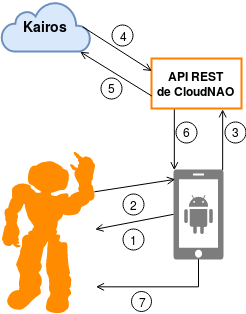
\includegraphics[scale=0.6]{study_case_kairos}
\end{figure}

\subsubsection{Reconocimiento óptico de caracteres y traducción de texto con Google Cloud Vision y Google Cloud Translation}

El reconocimiento óptico de caracteres (OCR por sus siglas en inglés) permite detectar y extraer texto de imágenes para luego
almacenarlo en un formato que una máquina pueda "entender".
La API de Vision de Google Cloud ofrece el servicio de OCR
que además incluye la detección del idioma en que se encuentra escrito.
Google Cloud cuenta también con una API para traducción de 
texto.
En la API REST de CloudNAO se combinan estos dos servicios
para añadir al robot NAO la funcionalidad de extracción y traducción de texto en imágenes. 

Esta característica dentro de CloudNAO sólo
se usa en la aplicación móvil, sin embargo, al igual que
la el reconocimiento de rostros, se puede utilizar directamente
sobre el robot. El usuario simplemente adquiere una fotografía
capturada por la cámara del robot y se hace la petición
a la API REST de CloudNAO que utiliza los servicios
de Google Cloud Vision y Translation para obtener el texto
y hacer la traducción, respectivamente.
Si existe texto en la imagen y fue correctamente procesado por
la API de Vision, éste se traduce, el resultado se muestra
en la aplicación y el robot repite oralmente
el texto traducido.

\subsubsection{Reconocimiento de voz con la API de Wit.ai}

Una aplicación interesante de tecnologías que realizan el 
procesamiento de lenguaje natural es la creación de bots conversacionales
o asistentes por voz. Wit.ai provee una API para contruir aplicaciones
con las que los usuarios se puedan comunicar a través de voz o texto.
El robot NAO es una plataforma con las características 
para interactuar de manera amigable, que a pesar de contar con un
módulo de reconocimiento de voz (\texttt{ALSpeechRecognition}), éste es muy 
básico y limitado.

Las aplicaciones desarrollados con Wit.ai aprenden conforme reciban más 
información, se vuelven más inteligentes con cada interacción de los usuarios.
En cambio, una aplicación usando sólo el módulo de \texttt{ALSpeechRecongnition} es estática.

Por todas estas razones se creó una aplicación sencilla
para interactuar con el robot usando el servicio \texttt{speech} de
Wit.ai.
Dentro de la API REST de CloudNAO existe un módulo para hacer las peticiones
a la API de Wit.ai; éste también puede usarse directamente sobre
el robot, evitando un intermediario.
Se solicita el recurso \texttt{speech} de la API de Wit.ai 
enviando
un archivo de audio generado por el robot. La API
envía como respuesta un JSON con la transcripción del audio 
en texto, las entidades e intenciones encontradas.
El robot es quien se encarga de manejar el flujo de
acciones dependiendo de las entidades.

Las entidades de una aplicación se definen en la plataforma
web de Wit.ai. Ésta cuenta con una herramienta para
crear entidades a partir de oraciones que el usuario
posiblemente enviará en un mensaje. Por ejemplo,
cuando el usuario inicie una conversación posiblemente
se con un "Hola", por lo que podemos definir una
entidad \texttt{saludo} con el valor \texttt{hola}.
Se pueden añadir más sentencias que el usuario
pueda decir cuando quiera saludar como "Buenas tardes",
"Buena día" y la entidad seguirá siendo saludo.
A partir de esto podemos definir acciones muy simples
para el robot guiadas por las entidades. En la
siguiente lista se describen las entidades que se
definieron para esta aplicación, qué acción realiza el robot
y un ejemplo de lo que puede decir el usuario para ejecutarla:


\begin{itemize}
\item  \texttt{walk}: El robot camina una pequeña distancia. "Levántate y anda."
\item \texttt{restPosition}: El robot cambia a una posición de descanso (crouch). "Descansa robot".
\item \texttt{greeting}: El robot realiza un gesto y saluda al usuario."Hola robot".
\item \texttt{photography}: El robot toma una fotografía y la almacena en su disco. "Toma una foto de lo que ves".
\item \texttt{sayGoodbye}: El robot se despide del usuario y termina la aplicación. "Adiós robot".
\item \texttt{animation}: El robot ejecuta una animación aleatoria.
"Robot, dame un movimiento sorpresa".
\item \texttt{textDetection}: Utilizando la API de Vision de Google Cloud
el robot extrae texto de una imagen y lo expresa oralmente. "Lee que dice
aquí".
\end{itemize}

La aplicación se puede volver tan compleja como se desee,
el añadir más entidades hace más interesante intectuar con el
robot. Podemos agregar otros servicios para
que cada vez se parezca más a un asistente por voz,
como los calendarios y contactos de Google, la búsqueda de lugares y
zonas de interés con servicios como Foursquare o los Mapas de Google,
uso de la la gráfica de conocimiento de Google o de Wolfram Alpha, 
servicios de noticias, etc.

\begin{figure}[!h]
\centering
\caption{El funcionamiento de la interacción con el robot a través de un discurso
oral. 1) El usuario envía un mensaje que el robot graba en un archivo de audio
con unos cuantos segundo de duración. 2) El robot procesa envía el archivo de audio
a la API de Wit.ai. 3) Wit.ai envía un JSON con las entidades encontradas. El robot realiza una acción dependiendo de las entidades.}
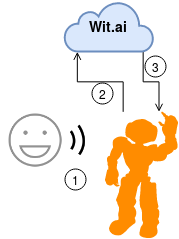
\includegraphics{study_case_wit}
\end{figure}



Este capítulo se describieron cada uno de los
componentes de la arquitectura de software CloudNAO.

De la API REST se mostraron los recursos que ofrece, como enviar una solicitud y la estructura de la respuesta 
retornada por la API. Además, se incluye una descripción
de cada módulo que compone la aplicación para poder
darle mantenimiento, replicarla o extenderla.

Después se incluye un apartado únicamente para
hablar de la base de datos en tiempo real de Firebase
y su papel dentro de CloudNAO. Aquí se definió 
la estructura del JSON y cada uno de sus atributos.

De la aplicación móvil para dispositivos con
sistema Android se exponen las funcionalidades que 
ofrece y también una explicación general de las 
clases principales dentro del código fuente.

Además se incluye un apartado especial de la conexión 
del robot NAO con Firebase sin ningún intermediario








% %%%%%%%%%%%%%%%%%%%%%%%%%%%%%%%%%%%%%%%%%%%%%%%%%%%%%%%
% %%%%%%%%%%%%%%%%%%%%%%%%%%%%%%%%%%%%%%%%%%%%%%%%%%%%%%%
% %%%%%%%% Capítulo 3 : Servicio en la nube %%%%%%%%%%%%%
% %%%%%%%%%%%%%%%%%%%%%%%%%%%%%%%%%%%%%%%%%%%%%%%%%%%%%%%
% %%%%%%%%%%%%%%%%%%%%%%%%%%%%%%%%%%%%%%%%%%%%%%%%%%%%%%%

\chapter{Un servicio de cómputo en la nube sobre la arquitectura CloudNAO}
\label{\detokenize{chapter_three:un-servicio-de-computo-en-la-nube-sobre-la-arquitectura-cloudnao}}
\label{\detokenize{chapter_three::doc}}


% %\documentclass[10pt,a4paper]{article}
%\usepackage[utf8]{inputenc}
%\usepackage{amsmath}
%\usepackage{amsfonts}
%\usepackage{amssymb}
%\begin{document}
%

El segundo objetivo del
trabajo es implementar un modelo de aprendizaje 
profundo que se brinde como un servicio web para ser consumido por robots NAO.
A pesar de que el servicio de detección de objetos es mantenido por el LAR, y 
se adaptó para ser consumido a través de la API REST, no fue construido
desde cero ya que es parte de la API de detección de objetos de TensorFlow.
Es por eso que como parte final del proyecto se desarrolló un modelo que 
resolviera la tarea de clasificar imágenes.

El problema de clasificación de imágenes es la tarea de asignarle a una imagen de
entrada una etiqueta a partir de un conjunto de categorías. Éste es uno de los principales
problemas dentro del campo de la visión computacional, que a pesar de su simplicidad
tiene bastantes aplicaciones prácticas. Entre esas aplicaciones, muchas interesan al
campo de la robótica móvil, por ejemplo, para la navegación de un robot de manera
autónoma, nos gustaría que supiera en que lugar está simplemente con una fotografía
que obtenga en ese momento, así podría saber si ha llegado al 
lugar de su objetivo, o a partir de la zona donde se ubica planear una trayectoria.

Lo anterior nos inspiró en la creación de un modelo que clasificara imágenes
de algunos lugares sobre los que podría navegar el robot NAO. 
Como solución a este problema de clasificación se propuso usar 
una red neuronal convolucional, que recibiera como entrada un arreglo con los
pixeles de una imagen tomada por el robot, y la salida fuera la categoría
a la que pertenece esa imagen. 
Las clases en las que se desea clasificar las imágenes son lugares alrededor
del Laboratorio de Algoritmos para la Robótica, que se ubica en el cubículo $15$ del
Centro de Desarrollo Tecnológico de la FES Acatlán. Se eligieron las siguientes cuatro zonas:

\begin{itemize}
    \item El cubículo.
    \item La salida de emergencia.
    \item La cancha de entrenamiento de fútbol para el robot NAO.
    \item Zona de trabajo del Laboratorio.
\end{itemize}


En este capítulo se describe con detalle la confección del
conjunto de datos, la arquitectura de la red 
convolucional, la implementación
del modelo utilizando Python y TensorFlow, los resultados obtenidos
y finalmente cómo se integra este modelo dentro de la API de CloudNAO 

%
%\end{document}
% %\documentclass[10pt,a4paper]{book}
%\usepackage[utf8]{inputenc}
%\usepackage{amsmath}
%\usepackage{amsfonts}
%\usepackage{amssymb}
%\usepackage{graphicx} 
%
%
%\begin{document}
%En esta sección se describe la preparación del conjunto de datos, 
%la selección de la estructura y los parámetros del modelo de aprendizaje profundo.

\section{Descripción del servicio sobre CloudNAO}


\subsection{Descripción del conjunto de datos\label{sec:dataset-def}}

Son cuatro las categorías en las que se quiere
clasificar una imagen obtenida por el robot: el cubículo,
la salida de emergencia, la cancha de fútbol y la zona de trabajo.

\begin{figure}[ht]
    \centering
    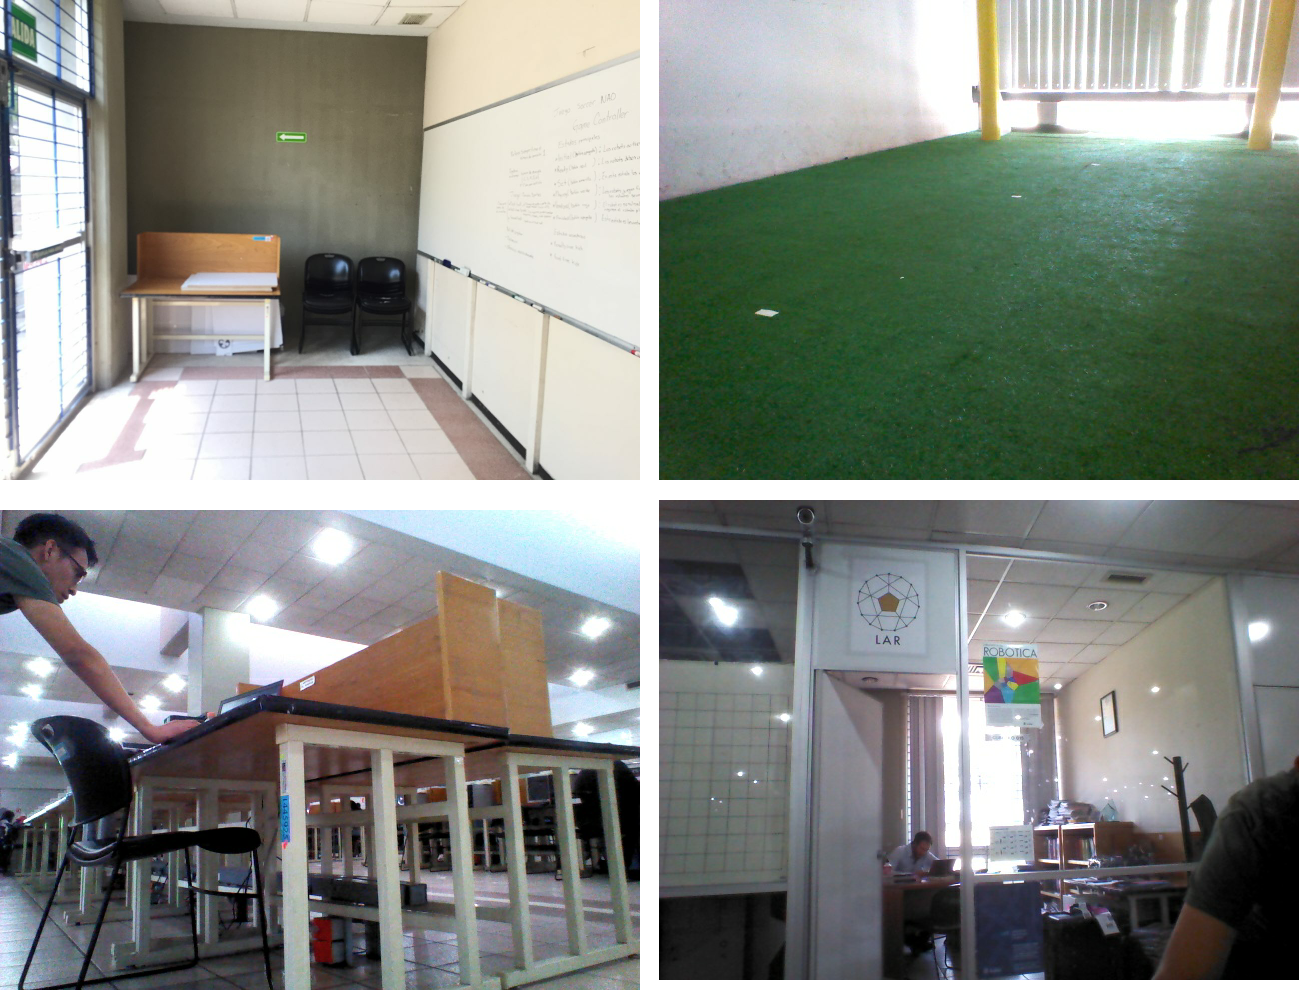
\includegraphics[width=0.5\textwidth]{scenes.png}
    \caption{Fotografías de las cuatro zonas dentro del laboratorio. De izquierda a derecha y
    de arriba a abajo: salida, cancha, zona de trabajo y cubículo.
    }
    \label{fig:scenes}
\end{figure}

Las imágenes se obtuvieron desde el robot usando el módulo de
\texttt{ALVideoRecorder},
el cual permite guardar secuencias de video utilizando las cámaras del robot y guardarlas 
en su disco. De los videos se extrajeron algunos fotogramas, no todos para evitar
redundancias, los cuales se separaron en carpetas
de acuerdo al lugar (categoría) que pertenecían. Después de este proceso
de obtención de imágenes a partir de video y de su separación en cada clase, se
generaron dos conjuntos, el de entrenamiento y el de prueba. El conjunto 
de entrenamiento está compuesto por $6000$ imágenes, $1500$ por cada clase.
El conjunto de prueba contiene $2112$ imágenes, $528$ por cada categoría.
En ambos conjuntos cada imagen es de $60 \times  80$ pixeles y de tres canales por ser imágenes en el modelo de color RGB.



\subsection{Arquitectura de la CNN}

La selección de una arquitectura para la CNN y de sus parámetros se
realizó a través de pruebas. Se tomó como base 
la arquitectura LeNet-5 (una variante de la arquitectura LeNet  que fue una de las primeras CNN que operaba sobre el 
conjunto MNIST de dígitos escritos a mano) y se probó cambiando
diversos parámetros como el número y tamaño de los kernels, la tasa de aprendizaje y el número de unidades en las capas completamente conectadas.

El primer parámetro importante son las dimensiones de
la entrada de la red. El valor de éste se mantuvo del
modelo LeNet-5 donde las imágenes tiene tamaño de $32 \times 32$,
con la adición de que las imágenes en nuestra red
tienen tres canales porque se encuentran en el espacio de 
color RGB.

\begin{figure}[!ht]
\centering
\caption{Arquitectura LeNet-5}
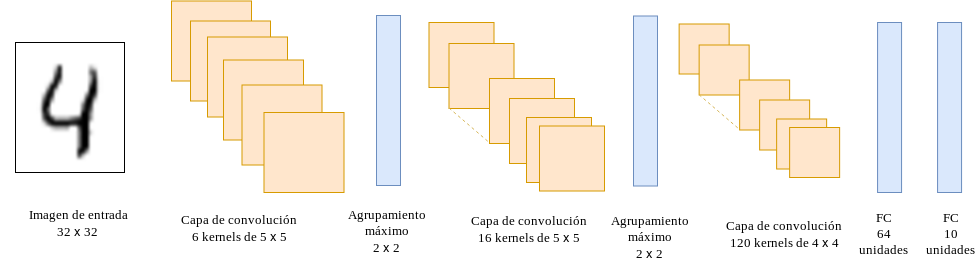
\includegraphics[scale=0.4]{lenet}
\end{figure}

LeNet-5 consiste de dos capas de convolución seguidas de dos
capas completamente conectadas, donde la última produce
la salida de la red.
Por facilidad sólo se experimentó con modelos de una y dos capas
de convolución. Las dimensiones de los kernels  que se probaron fueron de 
$7 \times 7$,
$5 \times 5$ y $3 \times 3$. En el caso de los modelos con
dos capas de covolución se pusieron por pares los tamaños de
los kernels; $7 \times 7$ con
$5 \times 5$, y $5 \times 5$ con $3 \times 3$, donde los kernels
de dimensión mayor iban en la primera capa de convolución.
Para estructuras con una capa de convolución los kernels
se mantuvieron con una dimensión de $5 \times 5$.
El número de mapas de características que se deberían producir
en cada capa de convolución se tomó de entre los valores: $8$, 
$16$, $32$, emparejando $8$ con $16$ y $16$ con $32$.
Donde $8$ y $16$ son el número de mapas obtenidos de la primera 
capa de convolución y $16$ y $32$ para la segunda.
Queremos mantener el tamaño de los mapas de
características del mismo que el de las entradas de la convolución,
esto se logra con un borde de ceros llamado \textit{same}, 
el cual se asegura que las salidas y entradas tengan las mismas dimensiones. 
La zancada o stride se mantiene constante con un valor de $1$.
Para la parte del pooling queremos ir disminuyendo las 
dimensiones de las entradas a la mitad después de cada
convolución, por lo que se ocupa un agrupamiento máximo 
de $2 \times 2$.


En cuanto a las capas completamente conectadas, se evaluaron
modelos con una capa oculta y una capa de salida y estructuras
con únicamente la capa de salida. El número de unidades 
en la capa oculta se escogió de entre los valores $1024$,
$512$ y $128$. En la capa de salida la primera unidad corresponde a la
categoría de \textit{zona de trabajo}, la segunda a 
\textit{salida de emergencia}, la tercera a \textit{cubículo}
y la última a \textit{cancha de fútbol}.

La función de activación que se utiliza en la capa de
convolución es la función ReLU. En las arquitecturas con
una capa oculta, la salida de ésta también se pasa 
por una función de activación ReLU. Para la salida 
de la red, queremos una distribución de probabilidad
sobre un conjunto de etiquetas mutuamente excluyentes.
Esto es, queremos que la salida de la unidad $i$ en la capa
de salida nos de la probabilidad $p_i$ de que una imagen que
entra
a la red pertenezca a la categoría $i$. Para nuestro caso en específico
la salida sería un vector $\mathbf{p} = (p_1, p_2, p_3, p_4)$ donde $\sum_{i = 1}^4 p_i = 1$.
El cálculo de los valores de $\mathbf{p}$  se logra usando una la función \textit{softmax}.\\

\begin{remark}

La función softmax se emplea para mapear un vector $\mathbf{z} \in \mathbb{R}^k$,  en un vector $\sigma(\mathbf{z})$ de dimensión $k$ de valores reales en el rango $(0, 1]$ cuya suma es igual a $1$. La función está dada por: 
\end{remark}

\[
\sigma : \mathbb{R}^k \rightarrow \bigg \{ \sigma \in \mathbb{R}^k | \sigma_i > 0, \sum_{i=1}^k \sigma_i = 1 \bigg \}
\]

\[
\sigma(\mathbf{z})_j = \frac{e^{z_j}}{\sum_{i=1}^k e^{z_i}} \text{ para  } j=1,\dots,k
\]
%
%donde $\hat{p}_n$ es el resultado de la unidad de cómputo antes de pasarlo
%por una función de activación, es decir, no normalizado. Es claro
%que para esta función se necesitan los valores no normalizados
%de las otras unidades en la misma capa.

El tipo de función de costo depende principalmente de la tarea a realizar,
para nosotros una tarea de clasificación en múltiples clases. La función
de costo asociada con este problema es la \textit{entropía cruzada}.\\

\begin{remark}
La entropía cruzada mide la diferencia entre dos distribuciones de probabilidad, y está
definida como sigue:

\[
L(\mathbf{y}, \mathbf{p}) = - \sum_{n} y_n log(p_n) \text{		} n \in [1,N]
\]

donde $\mathbf{y}$ denota la salida deseada y $\mathbf{p}$ contiene las probabilidades
para categoría. Si hay $N$ unidades en la capa de salida, entonces
$\mathbf{p}, \mathbf{y} \in \mathbb{R}^N$. $\mathbf{y}$ y $\mathbf{p}$ deben ser dos distribuciones de probabilidad.
\end{remark}


Por último se utiliza el algoritmo de retropropagación para
minimizar el error actualizando los pesos de los kernels y de las capas
completamente conectadas. El modo de actualización es por lotes, 
donde el tamaño de los lotes fue de elegido entre los valores 
$100$, $200$ y $300$; y
para el número de épocas entre $500$, $1000$ y $2000$.
La tasa
de aprendizaje se tomó de entre las constantes $0.001$,
$0.001$ y $0.01$.

\begin{table}[]
\centering
\caption{Resumen de los parámetros del diseño de la CNN con los que se experimentó.}
\label{table:param_cnn}
\begin{tabular}{|l|l|}
\hline
Parámetro de diseño      & Valores probados                                                                                                                            \\ \hline
Capas                    & \begin{tabular}[c]{@{}l@{}}1 convolución 1 completa                    \\1 convolución 2 complestas\\ 2 convolución 1 completa\\ 2 convolución 2 completas\end{tabular} \\ \hline
\multicolumn{2}{|l|}{Capas de convolución}                                                                                                                             \\ \hline
Tamaño del kernel        & $7 \times 7$, $5 \times 5$, $3 \times 3$                                                                                                   \\ \hline
Borde de ceros                & Same                                                                                                                                        \\ \hline
Zancada                   & 1                                                                                                                                           \\ \hline
Mapas de características & 8, 16, 32                                                                                                                               \\ \hline
Pooling                  & \begin{tabular}[c]{@{}l@{}}Agrupamiento máximo (vecindades de \\ $2 \times 2$).\end{tabular}                                                \\ \hline
Función de activación    & ReLU                                                                                                                                        \\ \hline
\multicolumn{2}{|l|}{Capas completamente conectadas}                                                                                                                   \\ \hline
Salidas                  & 1024, 512, 128, 4                                                                                                                               \\ \hline
Funciones de activación  & ReLU y Softmax                                                                                                                              \\ \hline
\multicolumn{2}{|l|}{Aprendizaje}                                                                                                                                      \\ \hline
Función de costo         & Entropía cruzada                                                                                                                            \\ \hline
Optimizador              & Descenso de gradiente                                                                                                                       \\ \hline
Modo de actualización de pesos & Por lotes
\\ \hline
Tamaño del lote & 100, 200, 300
\\ \hline
Épocas & 500, 1000, 2000
\\ \hline
Tasa de aprendizaje & 0.0001, 0.001, 0.01
\\ \hline
\end{tabular}

\end{table}

A partir de estos parámetros se pueden formar $756$ arquitecturas distintas. 
La estructura de la red tiene cuatro formas posibles, dos capas de convolución
y dos completamente conectadas, dos de convolución y una completa, una de convolución
y dos completas y por último una de convolución y una completa. 

Para estructuras con dos capas de convolución y dos capas completamente conectadas 
tenemos dos
pares de dimensiones para el kernel y dos pares para el número de mapas de 
caracteríticas. Podemos escoger tres valores para el número de unidades 
en la cada oculta. Y tenemos tres valores distintos para la tasa de aprendizaje, 
el número de épocas y el tamaño del lote. Por lo que tenemos un total
de $2 \times 2 \times 3 \times 3 \times 3 \times 3 = 324$ modelos posibles. 

Para los siguientes casos: dos capas de convolución y una capa completamente conectada, una capa de convolución y dos capas completamente conectadas y
una capa de convolución y una capa completamente conectada, haciendo las
mismas operaciones tenemos $108$, $243$ y $81$ respectivamente.
Un ejemplo de una de las posibles arquitecturas se muestra en la figura \ref{fig:cnn_topo_example}.

\begin{figure}[!ht]
\centering
\caption{Ejemplo de una CNN con dos capas de convolucionales y dos completamente conectadas. El tamaño de los kernels en la primera capa de convolución es de $5 \times 5$ y de la segunda de
$3 \times 3$. Los mapas de características que se obtienen de la primera y segunda capa de convolución son $8$ y $16$, respectivamente. Se utiliza un agrupamiento máximo
para reducir el tamaño de la imagen de entrada hasta un $75$ porciento. Finalmente la capa oculta conectada con la capa de salida cuenta con $1024$ unidades.\label{fig:cnn_topo_example}}
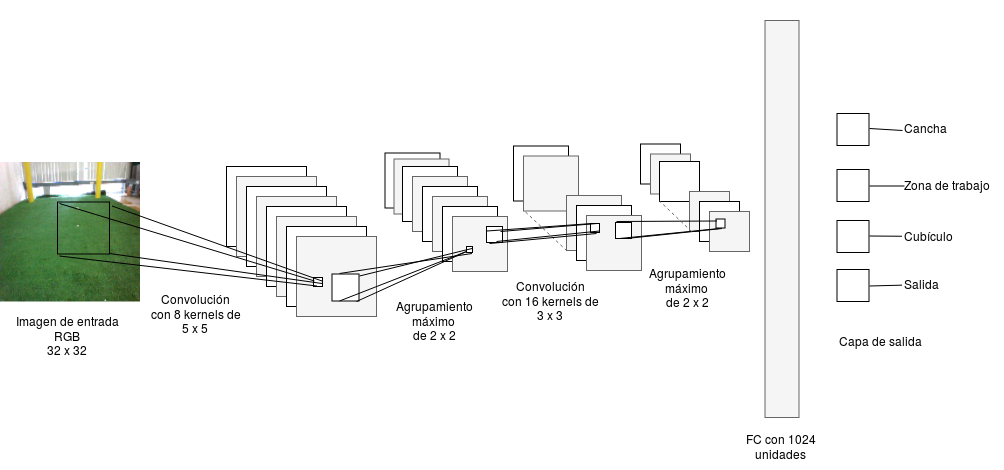
\includegraphics[scale=0.4]{cnn_topology_example}
\end{figure}
%\end{document}

% %		\def\sphinxdocclass{report}
%\documentclass[letterpaper,10pt,spanish]{sphinxmanual}
%\ifdefined\pdfpxdimen
%   \let\sphinxpxdimen\pdfpxdimen\else\newdimen\sphinxpxdimen
%\fi \sphinxpxdimen=.75bp\relax
%
%\PassOptionsToPackage{warn}{textcomp}
%\usepackage[utf8]{inputenc}
%\ifdefined\DeclareUnicodeCharacter
% \ifdefined\DeclareUnicodeCharacterAsOptional
%  \DeclareUnicodeCharacter{"00A0}{\nobreakspace}
%  \DeclareUnicodeCharacter{"2500}{\sphinxunichar{2500}}
%  \DeclareUnicodeCharacter{"2502}{\sphinxunichar{2502}}
%  \DeclareUnicodeCharacter{"2514}{\sphinxunichar{2514}}
%  \DeclareUnicodeCharacter{"251C}{\sphinxunichar{251C}}
%  \DeclareUnicodeCharacter{"2572}{\textbackslash}
% \else
%  \DeclareUnicodeCharacter{00A0}{\nobreakspace}
%  \DeclareUnicodeCharacter{2500}{\sphinxunichar{2500}}
%  \DeclareUnicodeCharacter{2502}{\sphinxunichar{2502}}
%  \DeclareUnicodeCharacter{2514}{\sphinxunichar{2514}}
%  \DeclareUnicodeCharacter{251C}{\sphinxunichar{251C}}
%  \DeclareUnicodeCharacter{2572}{\textbackslash}
% \fi
%\fi
%\usepackage{cmap}
%\usepackage[T1]{fontenc}
%\usepackage{amsmath,amssymb,amstext}
%\usepackage{babel}
%\usepackage[Sonny]{fncychap}
%\usepackage{sphinx}
%
%\usepackage{breakurl}
%\usepackage{geometry}
%
%% Include hyperref last.
%\usepackage{hyperref}
%% Fix anchor placement for figures with captions.
%\usepackage{hypcap}% it must be loaded after hyperref.
%% Set up styles of URL: it should be placed after hyperref.
%\urlstyle{same}
%\addto\captionsspanish{\renewcommand{\contentsname}{Contents:}}
%
%\addto\captionsspanish{\renewcommand{\figurename}{Figura}}
%\addto\captionsspanish{\renewcommand{\tablename}{Tabla}}
%\addto\captionsspanish{\renewcommand{\literalblockname}{Lista}}
%
%\addto\captionsspanish{\renewcommand{\literalblockcontinuedname}{proviene de la página anterior}}
%\addto\captionsspanish{\renewcommand{\literalblockcontinuesname}{continues on next page}}
%
%\addto\extrasspanish{\def\pageautorefname{página}}
%

%\begin{document}

\section{Implementación del servicio sobre CloudNAO}



Para crear y probar cada una de las arquitecturas que se
describieron en la sección anterior se utilizó la biblioteca
de TensorFlow.
Se construyó una clase que pudiera crear gráficas de modelos
con los cuatro casos antes descritos y luego se automatizó el proceso de
entrenamiento de todas las posibles arquitecturas, variando los parámetros.
Así, cada instancia de la clase, es un modelo diferente. En esta sección se 
describe la implementación de las CNN, su entrenamiento, evaluación
y lanzamiento sobre la API REST de CloudNAO.


El programa en TensorFlow encargado del entrenamiendo de la CNN se puede dividir en tres partes principales; la primera es la carga las imágenes de cada conjunto a partir de su ruta y su etiquetado, en la segunda
se crean las gráficas de cómputo y por último se ejecutan esas gráficas de cómputo.

Para agregar el modelo a la API de CloudNAO sólo se añadió un nuevo módulo
al recurso \texttt{/vision}, en donde se carga la gráfica de cómputo 
con los mejores resultados.

%%%%%%%%%%%%%%%%%%%%%%%%%%%%%%%%%%%%%%%%%%%%%%%%%%%%%%%%%%%%%%%%
%%%%%%%%%%%%%%%%%%%%%%%%%%%%%%%%%%%%%%%%%%%%%%%%%%%%%%%%%%%%%%%%
%%%%%%%%%%%%%%%%%%%%%%%%%%%%%%%%%%%%%%%%%%%%%%%%%%%%%%%%%%%%%%%%


\subsection{Hardware y software}

El hardware sobre el que se realizó el entrenamiento de las
diferentes arquitecturas fue un equipo con las siguientes características:

\begin{itemize}

\item Procesador: Intel Core i5-7300HQ CPU 2.50GHz x 4.
\item Memoria RAM: 8GB.
\item GPU:  NVIDIA GeForce GTX 1050 2GB.
\item SSD: 250 GB.
\end{itemize}

Como ya se explicó, la biblioteca para desarrollar el modelo en Python fue TensorFlow, la cual cuenta
con soporte para la plataforma de cómputo paralelo CUDA (Arquitectura
Unificada de Dispositivos de Cómputo), desarrollada por NVIDIA.
La versión de CUDA y de TensorFlow (con sopore para GPU) fueron 8.0 y 1.4.0, respectivamente.

Además de TensorFlow, las otras dos bibliotecas importantes son 
\texttt{numpy} y \texttt{opencv}, principalmente para la carga de
las imágenes en un formato que pudiera recibir la CNN.


%%%%%%%%%%%%%%%%%%%%%%%%%%%%%%%%%%%%%%%%%%%%%%%%%%%%%%%%%%%%%%%%%%%%%%%%%%%%%%%%%%%%%%%%%%%%%%%%%%%%%%%%%%%%%%%%%%%%%%%%%%%%%%%%%%%%%%%%%%%%%%%%%%%%%%%%%%%%%%%%%%%%%%%%%%%%%%%%%%%%%%%%%%%%%%%%%%%%%%%%%%%%%%%%%
\subsection{Preparación del conjunto de datos}

Contamos con un conjunto de entrenamiento de $6000$ imágenes y 
un conjunto de prueba de $2112$.
Como estamos utilizando un algoritmo de aprendizaje supervisado, 
se necesitan etiquetas u objetivos para cada imagen. La representación
de esas etiquetas se hizo con vectores $\mathbf{y}$ en codificación one-hot,
con $y_n = 1$ si la imagen pertenece a la clase $n$ y $y_i = 0$ para todos los
demás casos. Los vectores posibles de acuerdo las cuatro categorías son los siguientes:

\begin{itemize}
\item $(1, 0, 0, 0)$ si la imagen es de la categoría \textit{zona de trabajo}.
\item $(0, 1, 0, 0)$ si la imagen es de la categoría \textit{salida}.
\item $(0, 0, 1, 0)$ si la imagen es de la categoría \textit{cubículo}.
\item $(0, 0, 0, 1)$ si la imagen es de la categoría \textit{cancha}.
\end{itemize}

Esta codificación se puede intepretar como una distribución de probabilidad
sobre las cuatro clases.

Se definió un módulo \texttt{cnn\_indoor\_classifier\_model} con 
una clase \texttt{CNNClassifierLAR}
que encapsula los métodos para la carga de las imágenes, su 
procesamiento, la definición de la gráfica de cómputo y la ejecución 
Dentro de la clase el método \texttt{get\_training\_and\_test\_images()}
carga y procesa las imágenes para definir los conjuntos de entrenamiento
y de prueba para nuestro modelo.
Primero se obtiene la ruta de cada imagen y se crea la lista con las etiquetas
(vectores one-hot)
de cada imagen dependiendo de la carpeta donde se encontraba, luego con
\sphinxcode{\sphinxupquote{opencv}} se cargan las imágenes a la memoria como arreglos de
\sphinxcode{\sphinxupquote{numpy}}, se redimensionan a un tamaño de 32 * 32 y se normalizan
los valores de los pixeles. Al final se tienen dos arreglos de \sphinxcode{\sphinxupquote{numpy}}
donde cada elemento es un arreglo de tres dimensiones que
representa una imagen. El código de las operaciones dentro del método
son las siguientes:

\fvset{hllines={, ,}}%
\begin{sphinxVerbatim}[commandchars=\\\{\}]
\PYG{c+c1}{\PYGZsh{} Carga del conjunto de entrenamiento}
\PYG{n}{training\PYGZus{}paths} \PYG{o}{=} \PYG{n}{np}\PYG{o}{.}\PYG{n}{array}\PYG{p}{(}\PYG{n}{list\PYGZus{}files\PYGZus{}in\PYGZus{}directory}\PYG{p}{(}\PYG{l+s+s1}{\PYGZsq{}}\PYG{l+s+s1}{dataset/training\PYGZus{}set/*}\PYG{l+s+s1}{\PYGZsq{}}\PYG{p}{)}\PYG{p}{)}
\PYG{n}{np}\PYG{o}{.}\PYG{n}{random}\PYG{o}{.}\PYG{n}{shuffle}\PYG{p}{(}\PYG{n}{training\PYGZus{}paths}\PYG{p}{)}
\PYG{n}{labels\PYGZus{}training\PYGZus{}set} \PYG{o}{=} \PYG{n}{get\PYGZus{}labels\PYGZus{}from\PYGZus{}path}\PYG{p}{(}\PYG{n}{training\PYGZus{}paths}\PYG{p}{)}
\PYG{n}{training\PYGZus{}images} \PYG{o}{=} \PYG{n}{np}\PYG{o}{.}\PYG{n}{array}\PYG{p}{(}\PYG{p}{[}\PYG{n}{cv2}\PYG{o}{.}\PYG{n}{cvtColor}\PYG{p}{(}\PYG{n}{cv2}\PYG{o}{.}\PYG{n}{resize}\PYG{p}{(}\PYG{n}{cv2}\PYG{o}{.}\PYG{n}{imread}\PYG{p}{(}\PYG{n}{file\PYGZus{}name}\PYG{p}{)}\PYG{p}{,} \PYG{p}{(}\PYG{l+m+mi}{32}\PYG{p}{,} \PYG{l+m+mi}{32}\PYG{p}{)}\PYG{p}{)}\PYG{p}{,} \PYG{n}{cv2}\PYG{o}{.}\PYG{n}{COLOR\PYGZus{}BGR2RGB}\PYG{p}{)} \PYG{o}{/} \PYG{l+m+mi}{255} \PYG{k}{for} \PYG{n}{file\PYGZus{}name} \PYG{o+ow}{in} \PYG{n}{training\PYGZus{}paths}\PYG{p}{]}\PYG{p}{)}
\PYG{c+c1}{\PYGZsh{} Conjunto de prueba}
\PYG{n}{testing\PYGZus{}paths} \PYG{o}{=} \PYG{n}{np}\PYG{o}{.}\PYG{n}{array}\PYG{p}{(}\PYG{n}{list\PYGZus{}files\PYGZus{}in\PYGZus{}directory}\PYG{p}{(}\PYG{l+s+s1}{\PYGZsq{}}\PYG{l+s+s1}{dataset/test\PYGZus{}set/*}\PYG{l+s+s1}{\PYGZsq{}}\PYG{p}{)}\PYG{p}{)}
\PYG{n}{np}\PYG{o}{.}\PYG{n}{random}\PYG{o}{.}\PYG{n}{shuffle}\PYG{p}{(}\PYG{n}{testing\PYGZus{}paths}\PYG{p}{)}
\PYG{n}{labels\PYGZus{}test\PYGZus{}set} \PYG{o}{=} \PYG{n}{get\PYGZus{}labels\PYGZus{}from\PYGZus{}path}\PYG{p}{(}\PYG{n}{testing\PYGZus{}paths}\PYG{p}{)}
\PYG{n}{testing\PYGZus{}images} \PYG{o}{=} \PYG{n}{np}\PYG{o}{.}\PYG{n}{array}\PYG{p}{(}\PYG{p}{[}\PYG{n}{cv2}\PYG{o}{.}\PYG{n}{cvtColor}\PYG{p}{(}\PYG{n}{cv2}\PYG{o}{.}\PYG{n}{resize}\PYG{p}{(}\PYG{n}{cv2}\PYG{o}{.}\PYG{n}{imread}\PYG{p}{(}\PYG{n}{file\PYGZus{}name}\PYG{p}{)}\PYG{p}{,} \PYG{p}{(}\PYG{l+m+mi}{32}\PYG{p}{,} \PYG{l+m+mi}{32}\PYG{p}{)}\PYG{p}{)}\PYG{p}{,} \PYG{n}{cv2}\PYG{o}{.}\PYG{n}{COLOR\PYGZus{}BGR2RGB}\PYG{p}{)} \PYG{o}{/}\PYG{l+m+mi}{255} \PYG{k}{for} \PYG{n}{file\PYGZus{}name} \PYG{o+ow}{in} \PYG{n}{testing\PYGZus{}paths}\PYG{p}{]}\PYG{p}{)}
\end{sphinxVerbatim}



%%%%%%%%%%%%%%%%%%%%%%%%%%%%%%%%%%%%%%%%%%%%%%%%%%%%%%%%%%%%%%%%%%%%%%
%%%%%%%%%%%%%%%%%%%%%%%%%%%%%%%%%%%%%%%%%%%%%%%%%%%%%%%%%%%%%%%%%%%%%%
%%%%%%%%%%%%%%%%%%%%%%%%%%%%%%%%%%%%%%%%%%%%%%%%%%%%%%%%%%%%%%%%%%%%

\subsection{Construcción del modelo en TensorFlow}
\label{\detokenize{model_desc:creacion-y-ejecucion-de-la-grafica-de-tensorflow}}

\subsubsection{Definición del modelo}

Para la implementación de la CNN en TensorFlow
se utilizó una clase que representara una
arquitectura. Esto fue para que experimentar con
una estructura y parámetros diferentes sólo
implicara instaciar un objeto de la clase.
La clase se llama \sphinxcode{\sphinxupquote{CNNClassifierLAR}} y
está dentro del módulo {\hyperref[\detokenize{model_desc:module-cnn\_indoor\_classifier\_model}]{\sphinxcrossref{\sphinxcode{\sphinxupquote{cnn\_indoor\_classifier\_model}}}}}.
El módulo anterior además de la clase contiene múltiples
funciones auxiliares para facilitar la definición
de los parámetros de aprendizaje, la operaciones entre los
tensores, la obtención de las rutas de las imágenes
y la generación de los vectores one-hot de sus etiquetas.

Se pueden contruir hasta cuatro tipos distintos de
arquitecturas, con dos capas convolucionales con una o dos
completamente conectadas, y con una capa de convolución
y uno o dos completamente conectadas.
La construcción de éstas se hace con los métodos
\texttt{create\_graph\_2\_convo\_layers()}
y \texttt{create\_graph\_1\_convo\_layer()}
que reciben como argumento una bandera para contruir su gráfica
de cómputo con dos o una capa completamente conectada. A
continuación se desglosan los pasos del método para
crear la gráfica con dos capas de convolución.

\begin{enumerate}

\item La creación de la primera de convolución, recibe como entradas el placeholder
con las imágenes y a la función se le pasan como parámetros una lista con las dimensiones
de los kernels que se aplican y el número de mapas de características. Por ejemplo
un lista \sphinxcode{\sphinxupquote{{[}5, 5, 3, 16{]}}} indica que se deben aplicar kernels de 5*5 a
una entrada con 3 canales (la imagen RGB), para obtener
16 mapas de características, después se aplica un agrupamiento para disminuir las
dimensiones de los 16 mapas a la mitad:

\fvset{hllines={, ,}}%
\begin{sphinxVerbatim}[commandchars=\\\{\}]
\PYG{n}{convo\PYGZus{}1} \PYG{o}{=} \PYG{n}{convolutional\PYGZus{}layer}\PYG{p}{(}\PYG{n}{input\PYGZus{}x\PYGZus{}ph}\PYG{p}{,} \PYG{n}{shape}\PYG{p}{)}
\PYG{n}{convo\PYGZus{}1\PYGZus{}pooling} \PYG{o}{=} \PYG{n}{max\PYGZus{}pool\PYGZus{}2by2}\PYG{p}{(}\PYG{n}{convo\PYGZus{}1}\PYG{p}{)}
\end{sphinxVerbatim}

\item Luego sigue la otra capa de convolución que tiene como entrada las salidas
de la capa anterior. Se aplica de nuevo un agrupamiento para reducir las al $50\%$ las
dimensiones de la imagen:

\fvset{hllines={, ,}}%
\begin{sphinxVerbatim}[commandchars=\\\{\}]
\PYG{n}{convo\PYGZus{}2} \PYG{o}{=} \PYG{n}{convolutional\PYGZus{}layer}\PYG{p}{(}\PYG{n}{convo\PYGZus{}1\PYGZus{}pooling}\PYG{p}{,} \PYG{n}{shape}\PYG{p}{)}
\PYG{n}{convo\PYGZus{}2\PYGZus{}pooling} \PYG{o}{=} \PYG{n}{max\PYGZus{}pool\PYGZus{}2by2}\PYG{p}{(}\PYG{n}{convo\PYGZus{}2}\PYG{p}{)}
\end{sphinxVerbatim}

\item Se redimensionan los
mapas de características para tener una red neuronal donde cada unidad es un
elemento dentro del mapa de características. Esto es equivalente a aplicar
una convolución con kernel de $1 \times 1$. 
Se conectan las unidades de la capa a una nueva capa oculta
completamente conectada.

\fvset{hllines={, ,}}%
\begin{sphinxVerbatim}[commandchars=\\\{\}]
\PYG{n}{convo\PYGZus{}2\PYGZus{}flat} \PYG{o}{=} \PYG{n}{tf}\PYG{o}{.}\PYG{n}{reshape}\PYG{p}{(}\PYG{n}{convo\PYGZus{}2\PYGZus{}pooling}\PYG{p}{,} \PYG{p}{[}\PYG{o}{\PYGZhy{}}\PYG{l+m+mi}{1}\PYG{p}{,} \PYG{l+m+mi}{8} \PYG{o}{*} \PYG{l+m+mi}{8} \PYG{o}{*} \PYG{n}{last\PYGZus{}maps\PYGZus{}of\PYGZus{}features}\PYG{p}{]}\PYG{p}{)}
\PYG{n}{full\PYGZus{}layer\PYGZus{}one} \PYG{o}{=} \PYG{n}{tf}\PYG{o}{.}\PYG{n}{nn}\PYG{o}{.}\PYG{n}{relu}\PYG{p}{(}\PYG{n}{normal\PYGZus{}full\PYGZus{}layer}\PYG{p}{(}\PYG{n}{convo\PYGZus{}2\PYGZus{}flat}\PYG{p}{,} \PYG{n}{units\PYGZus{}fc}\PYG{p}{)}\PYG{p}{)}
\end{sphinxVerbatim}

\item La última capa es el vector predicho, que se pasa por la función softmax para
medir el error con la entropía cruzada. Finalmente se tiene la operación
\sphinxcode{\sphinxupquote{train}} que minimiza la función de costo utilizando el algoritmo de
retropropagación:

\fvset{hllines={, ,}}%
\begin{sphinxVerbatim}[commandchars=\\\{\}]
\PYG{n}{y\PYGZus{}pred} \PYG{o}{=} \PYG{n}{tf}\PYG{o}{.}\PYG{n}{identity}\PYG{p}{(}\PYG{n}{normal\PYGZus{}full\PYGZus{}layer}\PYG{p}{(}\PYG{n}{full\PYGZus{}layer\PYGZus{}one}\PYG{p}{,} \PYG{l+m+mi}{4}\PYG{p}{)}\PYG{p}{)}
\PYG{n}{cross\PYGZus{}entropy} \PYG{o}{=} \PYG{n}{tf}\PYG{o}{.}\PYG{n}{reduce\PYGZus{}mean}\PYG{p}{(}\PYG{n}{tf}\PYG{o}{.}\PYG{n}{nn}\PYG{o}{.}\PYG{n}{softmax\PYGZus{}cross\PYGZus{}entropy\PYGZus{}with\PYGZus{}logits}\PYG{p}{(}\PYG{n}{labels}\PYG{o}{=}\PYG{n}{y\PYGZus{}true\PYGZus{}ph}\PYG{p}{,} \PYG{n}{logits}\PYG{o}{=}\PYG{n}{y\PYGZus{}pred}\PYG{p}{)}\PYG{p}{)}
\PYG{n}{optimizer} \PYG{o}{=} \PYG{n}{tf}\PYG{o}{.}\PYG{n}{train}\PYG{o}{.}\PYG{n}{GradientDescentOptimizer}\PYG{p}{(}\PYG{n}{learning\PYGZus{}rate}\PYG{o}{=}\PYG{n}{learning\PYGZus{}rate}\PYG{p}{)}
\PYG{n}{train} \PYG{o}{=} \PYG{n}{optimizer}\PYG{o}{.}\PYG{n}{minimize}\PYG{p}{(}\PYG{n}{loss}\PYG{o}{=}\PYG{n}{cross\PYGZus{}entropy}\PYG{p}{,} \PYG{n}{global\PYGZus{}step}\PYG{o}{=}\PYG{n}{tf}\PYG{o}{.}\PYG{n}{train}\PYG{o}{.}\PYG{n}{get\PYGZus{}global\PYGZus{}step}\PYG{p}{(}\PYG{p}{)}\PYG{p}{)}
\end{sphinxVerbatim}


\end{enumerate}


\subsubsection{Ejecución}

La ejecución de la gráfica de cómputo de una instancia
es con el método \texttt{run\_graph()}.
Se pasan como parámetro el número de épocas y el tamaño del lote
para el aprendizaje.
Este método ejecuta la operación
\sphinxcode{\sphinxupquote{train}} que a su vez corre todas las operaciones que la preceden.
Cada 100 épocas se evalúa la precisión del modelo y se imprimen:
el número de época, el tiempo transcurrido desde que se inició el entrenamiento, el error de entrenamiento, el error de prueba y
la precisión.


\codedocumentation{\sphinxbfcode{\sphinxupquote{class }}\sphinxcode{\sphinxupquote{cnn\_indoor\_classifier\_model.}}\sphinxbfcode{\sphinxupquote{CNNClassifierLAR}}{(\emph{shape\_convo\_layers}, \emph{units\_fc}, \emph{learning\_rate}})}

La clase que representa una arquitectura de red convolucional con a lo más
dos capas de convolución y dos capas completamente conectadas.

La red está creada para específicamente aceptar entradas de dimensiones
de 32 pixeles por 32 pixeles por 3 canales. El constructor recibe tres parámetros
una lista con las dimensiones de los kernels, entradas de la convolución y
número de mapas de características, un entero con el número de unidades en lax
capa oculta y un valor flotante que es la tasa de aprendizaje.
En el siguiente ejemplo se crea una red con dos capas de convolución,
una capa oculta con 2048 unidades y una tasa de aprendizaje de 0.01. La ejecución de la gráfica
para el aprendizaje por lotes recibe como parámetros 200 y 3000,
el tamaño del lote y el número de épocas, respectivamente.

\fvset{hllines={, ,}}%
\begin{sphinxVerbatim}[commandchars=\\\{\}]
\PYG{g+gp}{\PYGZgt{}\PYGZgt{}\PYGZgt{} }\PYG{k+kn}{from} \PYG{n+nn}{cnn\PYGZus{}indoor\PYGZus{}classifier\PYGZus{}model} \PYG{k}{import} \PYG{n}{CNNClassifierLAR}
\PYG{g+gp}{\PYGZgt{}\PYGZgt{}\PYGZgt{} }\PYG{n}{clasificador} \PYG{o}{=} \PYG{n}{CNNClassifierLAR}\PYG{p}{(}\PYG{p}{[}\PYG{p}{[}\PYG{l+m+mi}{5}\PYG{p}{,} \PYG{l+m+mi}{5}\PYG{p}{,} \PYG{l+m+mi}{3}\PYG{p}{,} \PYG{l+m+mi}{16}\PYG{p}{]}\PYG{p}{,} \PYG{p}{[}\PYG{l+m+mi}{3}\PYG{p}{,} \PYG{l+m+mi}{3}\PYG{p}{,} \PYG{l+m+mi}{16}\PYG{p}{,} \PYG{l+m+mi}{32}\PYG{p}{]}\PYG{p}{]}\PYG{p}{,} \PYG{l+m+mi}{2048}\PYG{p}{,} \PYG{l+m+mf}{0.01}\PYG{p}{)}
\PYG{g+gp}{\PYGZgt{}\PYGZgt{}\PYGZgt{} }\PYG{n}{clasificador}\PYG{o}{.}\PYG{n}{create\PYGZus{}graph\PYGZus{}2\PYGZus{}convo\PYGZus{}layers}\PYG{p}{(}\PYG{p}{)}
\PYG{g+gp}{\PYGZgt{}\PYGZgt{}\PYGZgt{} }\PYG{n}{clasificador}\PYG{o}{.}\PYG{n}{run\PYGZus{}graph}\PYG{p}{(}\PYG{l+m+mi}{200}\PYG{p}{,} \PYG{l+m+mi}{3000}\PYG{p}{)}
\PYG{g+go}{i; time; training loss; test loss; accuracy}
\PYG{g+go}{0;0.7688136100769043;1.5798137187957764;1.4590167999267578;0.13778409361839294}
\PYG{g+gp}{...}
\PYG{g+go}{3000;68.31876397132874;0.0036288381088525057;0.11022621393203735;0.9692234992980957}
\PYG{g+go}{Time 68.3188087940216}
\end{sphinxVerbatim}

%%%%%%%%%%%%%%%%%%%%%%%%%%%%%%%%%%%%%%%%%%%%%%%%%%%%%%%%%%%%%%%%%%%%%%%%%%%%%%%%%%%%%%%%%%%%%%%%%%%%%%%%%%%%%%%%%%%%%%%%%%%%%%%%%%%%%%%%%%%%%%%%%%%%%%%%%%%%%%%%%%%%%%%%%%%%%%%%%%%%%%%%%%%%%%%%%%%%%



\subsection{Resultados}

Los modelos con la precisión más alta de cada una de las cuatro estructuras mencionadas previamente se resumen en la tabla \ref{table:models_results}. Las abreviaciones Convo y FC denotan
a capas convolucionales y completamente conectadas, respectivamente.
$\gamma$ denota la tasa de aprendizaje, y el tiempo es la duración
del entrenamiento en segundos.

\begin{table}[!h]
\centering
\caption{Los modelos con la precisiones más altas en cada tipo de
estructura.\label{table:models_results}}

\begin{tabular}{|l|l|l|l|l|l|l|l|l|}
\hline
Modelo                                                           & Épocas & $\gamma$ & Lote & Kernels                                                              & \begin{tabular}[c]{@{}l@{}}Mapas\\ de\\ caracte-\\ rísticas\end{tabular} & \begin{tabular}[c]{@{}l@{}}Unidades\\ de la\\ capas\\ FC\end{tabular} & Precisión & Tiempo \\ \hline
\begin{tabular}[c]{@{}l@{}}(1) \\2 Convo\\ 2 FC\end{tabular} & 2000   & 0.01     & 200  & \begin{tabular}[c]{@{}l@{}}$5 \times 5$,\\ $3 \times 3$\end{tabular} & 16, 32                                                                   & 1024, 4                                                               & 0.97917   & 168.29 \\ \hline
\begin{tabular}[c]{@{}l@{}}(2)\\2 Convo\\2 FC\end{tabular}        & 2000   & 0.01     & 300  & \begin{tabular}[c]{@{}l@{}}$5 \times 5$,\\ $3 \times 3$\end{tabular} & 16, 32                                                                   & 1024, 4                                                               & 0.97917   & 191.71 \\ \hline
\begin{tabular}[c]{@{}l@{}}(3)\\2 Convo\\ 1 FC\end{tabular}  & 2000   & 0.01     & 300  & \begin{tabular}[c]{@{}l@{}}$7 \times 7$,\\ $5 \times 5$\end{tabular} & 16, 32                                                                   & 4                                                                     & 0.97159   & 79.73  \\ \hline
\begin{tabular}[c]{@{}l@{}}(4)\\1 Convo\\ 2 FC\end{tabular}  & 2000   & 0.01     & 200  & $5 \times 5$                                                         & 16                                                                       & 512, 4                                                                & 0.97775   & 119.13 \\ \hline
\begin{tabular}[c]{@{}l@{}}(5)\\1 Convo\\ 1 FC\end{tabular}  & 2000   & 0.01     & 100  & $5 \times 5$                                                         & 32                                                                       & 4                                                                     & 0.96117   & 45.83  \\ \hline
\end{tabular}

\end{table}

Los modelos con la mayor precisión sobre todos son el modelo uno y
dos con una proporción de valores correctamente clasficados de
0.97917. Se puede ver que los parámetros que comparten todas
las arquitecturas son el número de épocas y la tasa de aprendizaje,
además de que en sus kernels aparece al menos uno con una dimensión 
de $5 \times 5$.

\begin{figure}[!ht]
\renewcommand*\thesubfigure{\arabic{subfigure}} 
  \centering
\subfloat[2 Convo 2 FC]{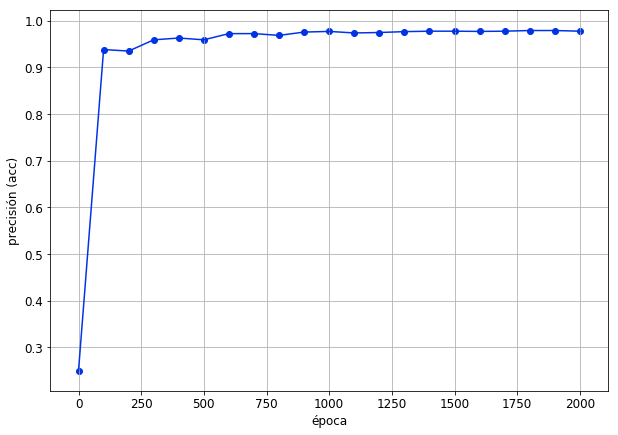
\includegraphics[scale=0.3]{model1}}
\qquad
\subfloat[2 Convo 2 FC]{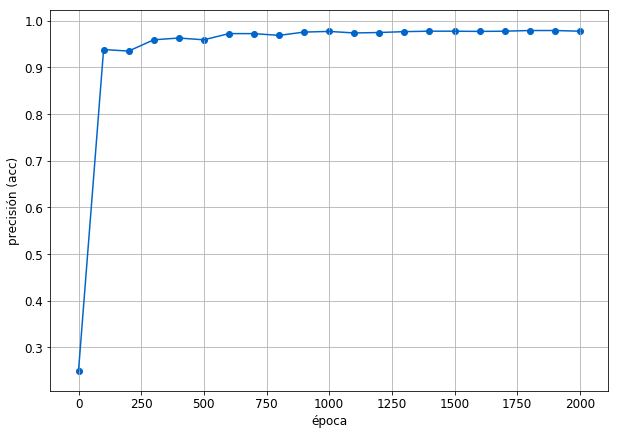
\includegraphics[scale=0.3]{model2}}
\qquad
\subfloat[2 Convo 1 FC]{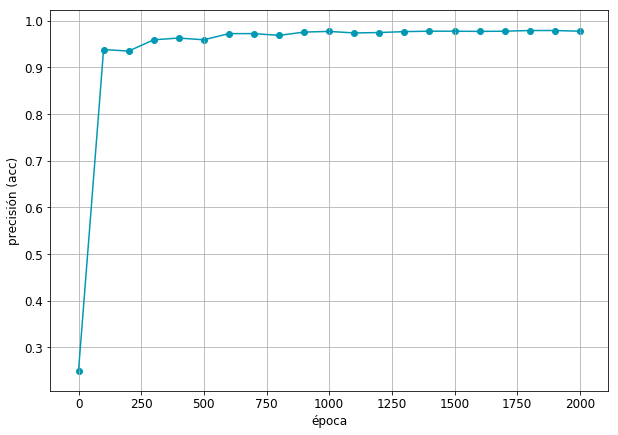
\includegraphics[scale=0.3]{model3}}
\qquad
\subfloat[1 Convo 2 FC]{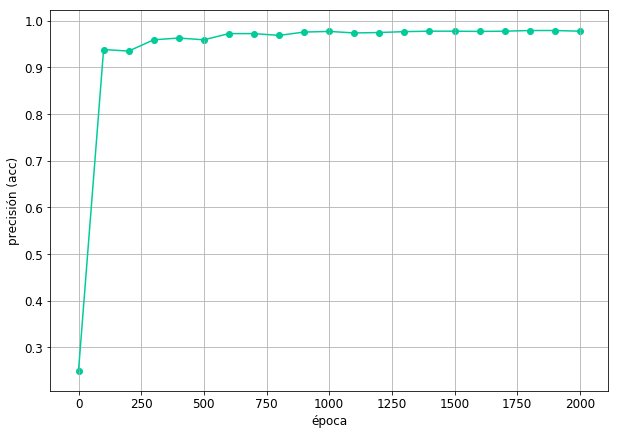
\includegraphics[scale=0.3]{model4}}
\qquad
\subfloat[1 Convo 1 FC]{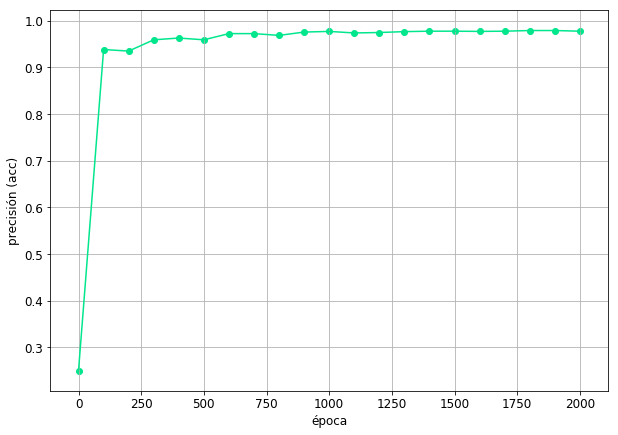
\includegraphics[scale=0.3]{model5}}
\caption{La precisión de cada modelo con respecto a las épocas.}
\end{figure}


%
%\paragraph{Modelo 1}
%
%2 convo 2 FC
%
%\begin{table}[]
%\centering
%\caption{Modelo 1: 2 capas de convolución y una capa oculta}
%\label{table:red_one_2conv2fc}
%\begin{tabular}{|l|l|l|l|l|}
%\hline
%Época & Tiempo transcurrido & Error de entrenamiento & Error de prueba & Precisión    \\ \hline
%0     & 7.3202745914        & 3.0709540844           & 6.1779737473    & 0.2504734993 \\ \hline
%100   & 15.3162293434       & 0.246046558            & 0.2345223427    & 0.9384469986 \\ \hline
%200   & 23.2666277885       & 0.2221536636           & 0.1732220352    & 0.9351325631 \\ \hline
%300   & 31.2877190113       & 0.115122892            & 0.1277082711    & 0.9592803121 \\ \hline
%400   & 39.3300793171       & 0.0641306639           & 0.1061202958    & 0.9630681872 \\ \hline
%500   & 47.3877923489       & 0.0945049077           & 0.1096037999    & 0.9592803121 \\ \hline
%600   & 55.337015152        & 0.04487269             & 0.0840779245    & 0.9725378752 \\ \hline
%700   & 63.4053928852       & 0.0290345363           & 0.0777522177    & 0.9725378752 \\ \hline
%800   & 71.4111871719       & 0.0502839647           & 0.0865348205    & 0.96875      \\ \hline
%900   & 79.4459328651       & 0.0260504074           & 0.0731359869    & 0.9758522511 \\ \hline
%1000  & 87.4989733696       & 0.0170939807           & 0.0684150234    & 0.9772727489 \\ \hline
%1100  & 95.6583366394       & 0.0299351327           & 0.073277019     & 0.9739583135 \\ \hline
%1200  & 103.6676399708      & 0.0175534561           & 0.0689379498    & 0.9749053121 \\ \hline
%1300  & 111.7657170296      & 0.0112776877           & 0.0651408285    & 0.9767992496 \\ \hline
%1400  & 119.8008499146      & 0.0180956665           & 0.0692276433    & 0.9777461886 \\ \hline
%1500  & 127.9180393219      & 0.0126623595           & 0.06640324      & 0.9777461886 \\ \hline
%1600  & 135.9379198551      & 0.0079146475           & 0.0643871278    & 0.9772727489 \\ \hline
%1700  & 144.0074915886      & 0.0117598884           & 0.0699412525    & 0.9777461886 \\ \hline
%1800  & 152.1184546947      & 0.0093412921           & 0.0654446557    & 0.9791666865 \\ \hline
%1900  & 160.2102677822      & 0.0058462457           & 0.064642258     & 0.9791666865 \\ \hline
%2000  & 168.2911362648      & 0.0085604852           & 0.0712103397    & 0.9777461886 \\ \hline
%\end{tabular}
%\end{table}
%
%\paragraph{Modelo 2}
%
%2 convo 2 FC.
%
%
%\begin{table}[]
%\centering
%\caption{Modelo 2: 2 capas de convolución y una oculta}
%\label{table:2conv2fcbatch300}
%\begin{tabular}{|l|l|l|l|l|}
%\hline
%Época & Tiempo transcurrido & Error de entrenamiento & Error de prueba & Precisión    \\ \hline
%0     & 7.8421280384        & 2.8682234287           & 3.3460187912    & 0.241477266  \\ \hline
%100   & 16.9836273193       & 0.3026786149           & 0.2827074528    & 0.9214015007 \\ \hline
%200   & 26.0736353397       & 0.1818257272           & 0.1859790981    & 0.9441288114 \\ \hline
%300   & 35.2737841606       & 0.1262233555           & 0.1477904469    & 0.9498106241 \\ \hline
%400   & 44.4421823025       & 0.1001303717           & 0.1264027655    & 0.9550189376 \\ \hline
%500   & 53.6251189709       & 0.0818474591           & 0.1112083346    & 0.9554924369 \\ \hline
%600   & 62.7804038525       & 0.0689618215           & 0.1012903452    & 0.9625946879 \\ \hline
%700   & 72.0268294811       & 0.0598993674           & 0.0959407836    & 0.9659090638 \\ \hline
%800   & 81.1530988216       & 0.0549877919           & 0.0937793404    & 0.9659090638 \\ \hline
%900   & 90.3930594921       & 0.0481151342           & 0.0898199677    & 0.9696969986 \\ \hline
%1000  & 99.5937502384       & 0.0406286344           & 0.085127607     & 0.9734848738 \\ \hline
%1100  & 108.7840344906      & 0.0342642255           & 0.08182735      & 0.9749053121 \\ \hline
%1200  & 117.9713246822      & 0.0278111324           & 0.0783735365    & 0.9767992496 \\ \hline
%1300  & 127.1896910667      & 0.0229252577           & 0.0762095153    & 0.9772727489 \\ \hline
%1400  & 136.4318993092      & 0.0191811435           & 0.0749697983    & 0.9782196879 \\ \hline
%1500  & 145.6369526386      & 0.0163648594           & 0.0740553215    & 0.9786931872 \\ \hline
%1600  & 154.8179557323      & 0.0139603755           & 0.0733383074    & 0.9791666865 \\ \hline
%1700  & 164.0475275517      & 0.0120949261           & 0.0730332807    & 0.9786931872 \\ \hline
%1800  & 173.2340805531      & 0.0105913281           & 0.0729769841    & 0.9772727489 \\ \hline
%1900  & 182.4875264168      & 0.0094167981           & 0.0730196685    & 0.9772727489 \\ \hline
%2000  & 191.7189230919      & 0.0084654102           & 0.0732315555    & 0.9772727489 \\ \hline
%\end{tabular}
%\end{table}
%
%\paragraph{Modelo 3}
%
%2 covo 1 FC.
%
%\begin{table}[]
%\centering
%\caption{Modelo 3: 2 capas de convolución 1 completamente conectada}
%\label{table:model3}
%\begin{tabular}{|l|l|l|l|l|}
%\hline
%Época & Tiempo transcurrido & Error de entrenamiento & Error de prueba & Precisión    \\ \hline
%0     & 2.1028752327        & 5.429710865            & 7.2814497948    & 0.2642045319 \\ \hline
%100   & 6.0483319759        & 0.3088294864           & 0.3315916061    & 0.9057765007 \\ \hline
%200   & 9.9446578026        & 0.207638666            & 0.2255852371    & 0.9289772511 \\ \hline
%300   & 13.8171753883       & 0.3040256202           & 0.2913019061    & 0.9005681872 \\ \hline
%400   & 17.6553535461       & 0.1283937991           & 0.1651451886    & 0.9427083135 \\ \hline
%500   & 21.5917801857       & 0.1089217067           & 0.157908693     & 0.9403409362 \\ \hline
%600   & 25.4469769001       & 0.1987725496           & 0.1853734255    & 0.9346590638 \\ \hline
%700   & 29.3310687542       & 0.0858137906           & 0.1235252693    & 0.9602272511 \\ \hline
%800   & 33.225922823        & 0.0737339705           & 0.1292105466    & 0.9535984993 \\ \hline
%900   & 37.1445102692       & 0.1441168338           & 0.1384231746    & 0.9521780014 \\ \hline
%1000  & 41.0286338329       & 0.0607568994           & 0.1053966731    & 0.9692234993 \\ \hline
%1100  & 44.9228360653       & 0.0545381755           & 0.1131819487    & 0.9621211886 \\ \hline
%1200  & 48.7702672482       & 0.1076918915           & 0.1140853167    & 0.9616477489 \\ \hline
%1300  & 52.6551091671       & 0.0456284918           & 0.0980426818    & 0.9701704383 \\ \hline
%1400  & 56.4932639599       & 0.0431456864           & 0.1037823632    & 0.9673295617 \\ \hline
%1500  & 60.3736059666       & 0.0825673938           & 0.1017076969    & 0.9668560624 \\ \hline
%1600  & 64.2060873508       & 0.0358270295           & 0.0946439132    & 0.9701704383 \\ \hline
%1700  & 68.1200900078       & 0.034217272            & 0.0975136459    & 0.9706439376 \\ \hline
%1800  & 72.0071187019       & 0.0638250113           & 0.0943133309    & 0.9701704383 \\ \hline
%1900  & 75.883657217        & 0.0286074877           & 0.0940102115    & 0.9711174369 \\ \hline
%2000  & 79.7310190201       & 0.0272229407           & 0.0934648365    & 0.9715909362 \\ \hline
%\end{tabular}
%\end{table}
%
%
%
%\paragraph{Modelo 4}
%
%1 convo 2 FC.
%
%
%\begin{table}[]
%\centering
%\caption{Tabla 4: 2 capas de convolución 1 completamente conectada.}
%\label{table:model4}
%\begin{tabular}{|l|l|l|l|l|}
%\hline
%Época & Tiempo transcurrido & Error de entrenamiento & Error de prueba & Precisión    \\ \hline
%0     & 4.8190894127        & 3.4078867435           & 1.8335254192    & 0.2561553121 \\ \hline
%100   & 10.5430588722       & 0.2876966596           & 0.2554202676    & 0.9190340638 \\ \hline
%200   & 16.2716712952       & 0.2585280836           & 0.1728164405    & 0.9441288114 \\ \hline
%300   & 21.984313488        & 0.2033729404           & 0.1497282833    & 0.9446022511 \\ \hline
%400   & 27.6639053822       & 0.133350119            & 0.139832899     & 0.9464961886 \\ \hline
%500   & 33.3875226974       & 0.1221942604           & 0.1160472557    & 0.9635416865 \\ \hline
%600   & 39.071198225        & 0.1346343458           & 0.111930415     & 0.9663825631 \\ \hline
%700   & 44.7847318649       & 0.0859281719           & 0.1102579832    & 0.9592803121 \\ \hline
%800   & 50.4557569027       & 0.0763712376           & 0.0923053026    & 0.9715909362 \\ \hline
%900   & 56.1923205853       & 0.0939286873           & 0.0953650922    & 0.9706439376 \\ \hline
%1000  & 61.9322435856       & 0.0572218187           & 0.0942356661    & 0.9678030014 \\ \hline
%1100  & 67.6439433098       & 0.0517053083           & 0.0810680985    & 0.9763257504 \\ \hline
%1200  & 73.3566286564       & 0.0669792295           & 0.0883587152    & 0.9730113745 \\ \hline
%1300  & 79.0891780853       & 0.0388560072           & 0.0845807865    & 0.9734848738 \\ \hline
%1400  & 84.7962470055       & 0.0358598083           & 0.07602036      & 0.9772727489 \\ \hline
%1500  & 90.4903838634       & 0.0488497727           & 0.0864205137    & 0.9725378752 \\ \hline
%1600  & 96.1585409641       & 0.0279216766           & 0.0798797309    & 0.9763257504 \\ \hline
%1700  & 101.8997781277      & 0.0248262715           & 0.0739214197    & 0.9777461886 \\ \hline
%1800  & 107.6456582546      & 0.0374025591           & 0.0860014334    & 0.9734848738 \\ \hline
%1900  & 113.370872736       & 0.0207491834           & 0.0776060075    & 0.9772727489 \\ \hline
%2000  & 119.1330387592      & 0.0177799109           & 0.0743050575    & 0.9767992496 \\ \hline
%\end{tabular}
%\end{table}
%
%\paragraph{Modelo 5}
%
%1 convo 1 FC.
%
%\begin{table}[]
%\centering
%\caption{Modelo 5: 1 capa de convolución 1 capa completamente conectada}
%\label{table:model5}
%\begin{tabular}{|l|l|l|l|l|}
%\hline
%Época & Tiempo transcurrido & Error de entrenamiento & Error de prueba & Precisión    \\ \hline
%0     & 1.3093357086        & 1.9210841656           & 1.9909992218    & 0.2334280312 \\ \hline
%100   & 3.5064704418        & 0.4699867666           & 0.3694962263    & 0.9019886255 \\ \hline
%200   & 5.718821764         & 0.2064059079           & 0.2735858858    & 0.9195075631 \\ \hline
%300   & 7.9507069588        & 0.321207583            & 0.2440538406    & 0.9180871248 \\ \hline
%400   & 10.1652519703       & 0.2827648222           & 0.2159627676    & 0.9261363745 \\ \hline
%500   & 12.399163723        & 0.1229303852           & 0.200532645     & 0.9313446879 \\ \hline
%600   & 14.6175277233       & 0.2280674428           & 0.192340821     & 0.9299242496 \\ \hline
%700   & 16.8630867004       & 0.2157354206           & 0.1778713614    & 0.9308711886 \\ \hline
%800   & 19.0751066208       & 0.0978225544           & 0.1696051657    & 0.9384469986 \\ \hline
%900   & 21.3231885433       & 0.1785159856           & 0.1666600704    & 0.9370265007 \\ \hline
%1000  & 23.5529901981       & 0.1691013724           & 0.1553606391    & 0.9427083135 \\ \hline
%1100  & 25.7864727974       & 0.0828434825           & 0.1507069916    & 0.9441288114 \\ \hline
%1200  & 28.0087628365       & 0.1457120925           & 0.1495355666    & 0.9450757504 \\ \hline
%1300  & 30.241517067        & 0.1372746676           & 0.1403872371    & 0.9493371248 \\ \hline
%1400  & 32.4557955265       & 0.0717598572           & 0.1377647668    & 0.9535984993 \\ \hline
%1500  & 34.7012207508       & 0.1211939454           & 0.1370747089    & 0.9507575631 \\ \hline
%1600  & 36.9285581112       & 0.1132190526           & 0.1292845905    & 0.9554924369 \\ \hline
%1700  & 39.1642153263       & 0.0621341504           & 0.1280657798    & 0.9569128752 \\ \hline
%1800  & 41.3848059177       & 0.1034243405           & 0.1276608855    & 0.9550189376 \\ \hline
%1900  & 43.6157948971       & 0.0946448147           & 0.120853819     & 0.9592803121 \\ \hline
%2000  & 45.837754488        & 0.055428572            & 0.1209859028    & 0.9611742496 \\ \hline
%\end{tabular}
%\end{table}
%
%%Los modelos con la mayor precisión sobre todos son el modelo uno y
%%dos con una proporción de valores correctamente clasficados del
%%0.9791666865. Se puede ver que los parámetros que comparten todas
%%las arquitecturas son el número de épocas y la tasa de aprendizaje,
%%además de que en sus kernels aparece al menos uno con una dimensión 
%%de $5 \times 5$.
%
%%
%%\end{document}


\subsubsection{Pruebas sobre el robot NAO}

Para finalizar la implementación del modelo sobre la arquitectura
se debe integrar uno de los cinco modelos descritos en la tabla \ref{table:models_results} sobre la API REST de CloudNAO y luego hacer peticiones con el robot a ésta.
Los modelos elaborados en TensorFlow contienen la gráfica de cómputo
y los valores de los parámetros que se han entrenado. Estos datos
están contenidos en varios archivos que se pueden guardar para
entrenamientos posteriores o para realizar inferencias sobre 
un modelo cuyas variables han sido aprendidas.

Se eligió el modelo con la precisión más alta y con el menor
tiempo de entrenamiento que es el modelo (1). 
%Durante la ejecución
%de la gráfica del modelo se crea una instancia de la clase \texttt{tf.train.Saver()}. Esto crea cuatro archivos
%uno con extensión \texttt{.meta}, uno con extensión \texttt{.index},
%otro con extensión \texttt{.data} y otro sin extensión llamado
%\texttt{checkpoint}. El primero guarda toda la gráfica de
%TensorFlow, los otros tres almacenan los valores de las variables.
%Después de guardar, simplemente se restaura el modelo
%y se puedan hacer inferencias al alimentarlo con una imagen.
Dentro de la API REST, la clase que se encarga de restaurar la gráfica y valores del modelo
es \texttt{ImageClasssfier} dentro del módulo \texttt{indoor\_scenes\_classsifier} del paquete \texttt{tf\_models}.
En el apartado \textit{Modelos de Tensorflow (tf\_models)}
de la sección \ref{chapter_two/desc_cloudnao:api-rest-de-cloudnao}
se describe cómo utilizar esta clase.

Por otra parte el robot NAO o cualquier otro
dispositivo cliente se comunica con la API a través
de una biblioteca que permita hacer peticiones 
HTTP. En el caso del robot ocupamos la biblioteca
\texttt{requests} de Python. Para obtener una imagen 
del robot codificada en base 64 se utilizó la clase \texttt{Robot}
del módulo \texttt{nao\_robot} descrito en la sección
\ref{\detokenize{firebase-nao-robot}}. Es la cadena
que representa la imagen la que se envía a la API REST usando
\texttt{requests}.

En la figura \ref{nao_api_images} se muestran algunas imagenes 
de $160 \times 120$ pixeles y las
respuestas enviadas por el servicio de clasificación
de escenarios dentro del recurso \texttt{vision} de la
API REST de CloudNAO.


\begin{figure}[!ht] 
  \centering
  
\subfloat[Clase = zona de trabajo, predicción = zona de trabajo. Tiempo = 3.02]{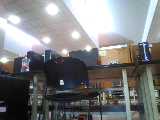
\includegraphics{nao_api_desk}}
\qquad
\subfloat[Clase = salida, predicción = salida. Tiempo = 3.12]{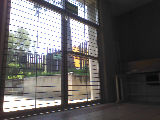
\includegraphics{nao_api_exit}}
\qquad
\subfloat[Clase = oficina, predicción = salida. Tiempo = 2.78]{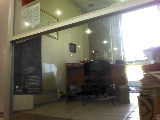
\includegraphics{nao_api_office}}
\qquad
\subfloat[Clase = cancha, predicción = cancha. Tiempo = 3.57]{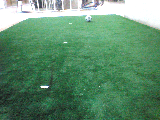
\includegraphics{nao_api_soccer}}
\caption{Predicciones hechas enviando imágenes del robot a la API REST. El tiempo son los
segundos que se tardó en enviar la solicitud y en recibir la respuesa. \label{nao_api_images}}
\end{figure}







 



% %%%%%%%%%%%%%%%%%%%%%%%%%%%%%%%%%%%%%%%%%%%%%%%%%%%%%%%
% %%%%%%%%%%%%%%%%%%%%%%%%%%%%%%%%%%%%%%%%%%%%%%%%%%%%%%%
% %%%%%%%%%%%%%%%%% Conclusiones %%%%%%%%%%%%%%%%%%%%%%%%
% %%%%%%%%%%%%%%%%%%%%%%%%%%%%%%%%%%%%%%%%%%%%%%%%%%%%%%%
% %%%%%%%%%%%%%%%%%%%%%%%%%%%%%%%%%%%%%%%%%%%%%%%%%%%%%%%


\chapter*{Conclusiones}
\label{\detokenize{conclusion:cloudnao-una-arquitectura-de-software-para-la-integracion-de-computo-en-la-nube-con-robots-nao}}\label{\detokenize{conclusion:conclusion}}\label{\detokenize{conclusion::doc}}
\addcontentsline{toc}{chapter}{Conclusiones}


El objetivo principal de esta tesis fue el diseño e 
implementación de
la arquitectura sobre la cual robots NAO pueden
utilizar tecnologías emergentes como son el cómputo en la nube
y el aprendizaje 
profundo. Esto se logró uniendo los siguientes componentes:
una aplicación móvil y una web, una API REST y al robot NAO.

En la aplicación
móvil se muestran algunos casos de uso del consumo de
servicios para que el robot NAO pueda realizar tareas
que por su capacidad de procesamiento no podría 
llevar a cabo de manera autónoma.
Con ésta, el robot puede generar datos que
se guardan en la nube o tomar una fotografía,
enviarla a un servicio para su procesamiento y a partir
de la respuesta obtenida realizar una acción; todo
esto en cuestión de segundos.
% Sin embargo, un problema pendiente de la aplicación móvil
% es la compatibilidad del SDK de NAOqi con nuevos sistemas
% Android.

Como los servicios brindados dentro de la arquitectura son 
RESTful, no están limitados a una sola plataforma
de consumo, cualquier dispositivo que pueda solicitar y
manejar mensajes HTTP puede hacer uso de los servicios
de la API REST de CloudNAO.
El papel de Firebase es importante porque muestra
los principales beneficios de la nube en el desarrollo
de aplicaciones modernas. Cuenta con una base de datos en tiempo
real que permite mandar comandos al robot de manera
inmediata, almacenar grandes volúmenes de datos
producidos por los sensores de éste y sincronizarlos entre los dispositivos
conectados.

Otra parte fundamental del trabajo fue el desarrollo
de una red neuronal convolucional para la clasificación
de imágenes en diferentes escenarios dentro del laboratorio.
De la experimentación, encontramos modelos
cuyo tiempo de entrenamiento es relativamente bajo, sólo unos 
cuantos pares de minutos, y cuya precisión es muy alta, que 
aunque no significa que sean excelentes clasificadores,
las pruebas sobre el robot funcionaron bien.
Esto en parte se debe a que
TensorFlow hace simples y eficientes
la definición, el entrenamiento y la carga de modelos de 
aprendizaje automático. 
% Un trabajo a futuro sería desarrollar un caso de estudio 
% donde el modelo sirva como auxiliar en la navegación
% del robot.

Como nota final puedo decir que las tecnologías empleadas
facilitan la adición
de nuevas funcionalidades sobre una plataforma con recursos
limitados, como los son los robots NAO,
permitiendo introducir al robot a otros campos de estudio.




% %%%%%%%%%%%%%%%%%%%%%%%%%%%%%%%%%%%%%%%%%%%%%%%%%%%%%%%
% %%%%%%%%%%%%%%%%%%%%%%%%%%%%%%%%%%%%%%%%%%%%%%%%%%%%%%%
% %%%%%%%%%%%%%%%%%%%% Anexos %%%%%%%%%%%%%%%%%%%%%%%%%%%
% %%%%%%%%%%%%%%%%%%%%%%%%%%%%%%%%%%%%%%%%%%%%%%%%%%%%%%%
% %%%%%%%%%%%%%%%%%%%%%%%%%%%%%%%%%%%%%%%%%%%%%%%%%%%%%%%


% 
\appendix
\clearpage
\addappheadtotoc
\appendixpage


\chapter{Herramientas para el desarrollo de la API REST\label{anexo:api-rest}}


\section*{Flask}
\label{\detokenize{chapter_two/desc_cloudnao:flask}}

Flask es un micro framework para desarrollo web. Fue diseñado para ser un
framework extensible, sólo provee un núcleo sólido con servicios básicos,
mientras que las extensiones brindan el resto. Esto quiere decir que Flask,
brinda la posibilidad contar sólo con las dependencias que se necesitan.

Tiene dos dependencias principales, \sphinxstylestrong{Werkzeug} y \sphinxstylestrong{Jinja2}.
El enrutamiento, debugging y WSGI tienen procedencia de Werkzeug.
Jinga2 ofrece el soporte para el manejo de plantillas. 
% Para nuestra
% aplicación solamente hacemos uso de la primera.

\begin{quote}

\sphinxstyleemphasis{WSGI} es la Web Server Gateway Interface. Es un protocolo que describe
cómo un servido web se comunica con aplicaciones web, y cómo las aplicaciones
web se pueden encadenar para procesar una petición.
\end{quote}

Para la instalación de Flask así como de cualquier paquete de Python, se
recomienda crear un ambiente virtual con la herramienta \sphinxstylestrong{virtualenv}.
Un ambiente virtual es una copia privada del intérprete de Python sobre la cual
es posible instalar paquetes de manera privada, sin afectar al intérprete
global de Python. Permite crear un ambiente de trabajo aislado para cada
proyecto, así cada aplicación tiene acceso solo a los paquetes que utiliza.
Con esto, lo descrito a continuación que se refiera a la instalación de
paquetes o ejecución de programas se
recomienda hacer dentro de un ambiente virtual.


\subsection*{Inicialización}
\label{\detokenize{chapter_two/desc_cloudnao:inicializacion}}
Todas las aplicaciones de Flask deben crear una \sphinxstyleemphasis{instancia de la aplicación}. Este
objeto maneja todas las peticiones que recibe el servidor web, usando
la especificación WSGI.
La instancia de la aplicación es un objeto de la clase \texttt{Flask},
se crea de la siguiente manera:

\begin{sphinxVerbatim}[commandchars=\\\{\}]
\PYG{k+kn}{from} \PYG{n+nn}{flask} \PYG{k}{import} \PYG{n}{Flask}
\PYG{n}{app} \PYG{o}{=} \PYG{n}{Flask}\PYG{p}{(}\PYG{n+nv+vm}{\PYGZus{}\PYGZus{}name\PYGZus{}\PYGZus{}}\PYG{p}{)}
\end{sphinxVerbatim}

El único argumento requerido para el constructor de la clase \texttt{Flask} es el nombre
del módulo o paquete de la aplicación. Para la mayoría de los casos,
la variable de Python \sphinxcode{\_\_name\_\_} es el valor correcto. Flask usa este argumento
para determinar la ruta raíz de la aplicación, para que después pueda encontrar
los archivos de los recursos relativos a la ubicación de la aplicación.


\subsection*{Rutas}
\label{\detokenize{chapter_two/desc_cloudnao:rutas}}
Los clientes envían peticiones al servidor web, que a su vez las envía a la
instancia de la aplicación de Flask. La instancia de la aplicación necesita saber
qué código debe regresar para cada URL solicitado, así que mantiene un mapeo de
los URL a funciones de Python. La asociación entre el URL y la función que se
la maneja se llama \sphinxstyleemphasis{ruta}.

La manera más conveniente de definir una ruta en una aplicación de Flask es
a través del decorador \sphinxcode{app.route}, que registra la función decorada como
una ruta.

El siguiente ejemplo registra la función \sphinxcode{index()} como el manejador para el URL
raíz de la aplicación. Si la aplicación fue desplegada en un servidor con el
nombre del dominio \sphinxurl{http://www.lar.com}. Al acceder desde un navegador a
la dirección anterior se ejecutará la función \sphinxcode{index()} del lado del servidor.
El valor
retornado por esta función se llama \sphinxstyleemphasis{respuesta}, y es lo que el cliente recibe.
Las funciones como \sphinxcode{index()} se llaman \sphinxstyleemphasis{funciones de vista}.
En este caso el navegador mostrará \sphinxcode{Hola mundo}.

\begin{sphinxVerbatim}[commandchars=\\\{\}]
\PYG{n+nd}{@app}\PYG{o}{.}\PYG{n}{route}\PYG{p}{(}\PYG{l+s+s1}{\PYGZsq{}}\PYG{l+s+s1}{/}\PYG{l+s+s1}{\PYGZsq{}}\PYG{p}{)}
\PYG{k}{def} \PYG{n+nf}{index}\PYG{p}{(}\PYG{p}{)}\PYG{p}{:}
  \PYG{k}{return} \PYG{l+s+s2}{\PYGZdq{}}\PYG{l+s+s2}{Hola mundo}\PYG{l+s+s2}{\PYGZdq{}}
\end{sphinxVerbatim}

Flask soporta los tipos de URL con componentes dinámicos utilizando
una sintaxis especial en el decorador \sphinxcode{route}. En el siguiente ejemplo se
muestra el nombre de usuario como componente dinámico.

\begin{sphinxVerbatim}[commandchars=\\\{\}]
\PYG{n+nd}{@app}\PYG{o}{.}\PYG{n}{route}\PYG{p}{(}\PYG{l+s+s1}{\PYGZsq{}}\PYG{l+s+s1}{/usuario/\PYGZlt{}nombre\PYGZgt{}}\PYG{l+s+s1}{\PYGZsq{}}\PYG{p}{)}
\PYG{k}{def} \PYG{n+nf}{user}\PYG{p}{(}\PYG{n}{nombre}\PYG{p}{)}\PYG{p}{:}
  \PYG{k}{return} \PYG{l+s+s2}{\PYGZdq{}}\PYG{l+s+s2}{Hola, }\PYG{l+s+si}{\PYGZob{}\PYGZcb{}}\PYG{l+s+s2}{\PYGZdq{}}\PYG{o}{.}\PYG{n}{format}\PYG{p}{(}\PYG{n}{nombre}\PYG{p}{)}
\end{sphinxVerbatim}

La parte encerrada por los paréntesis angulares es el componente dinámico, así
que cualesquiera URL que coincidan con la porción estática serán mapeadas a esta
ruta.

El decorador \sphinxcode{app.route} cuenta con el argumento opcional \sphinxcode{methods},
que recibe
una lista de métodos HTTP. \sphinxcode{methods} 
% le dice a Flask que 
registra las
funciones de vista como manejadores para las peticiones de acuerdo
al tipo de método enviado. Cuando \sphinxcode{methods} no está en los parámetros de la
función, la función de vista es registrada para manejar solamente peticiones
\sphinxcode{GET}. El siguiente ejemplo se le pide a Flask que se registre a la
función de vista como manejadora de petición de tipo \sphinxcode{GET} y \sphinxcode{POST}.

\begin{sphinxVerbatim}[commandchars=\\\{\}]
\PYG{n+nd}{@app}\PYG{o}{.}\PYG{n}{route}\PYG{p}{(}\PYG{l+s+s1}{\PYGZsq{}}\PYG{l+s+s1}{/usuario/\PYGZlt{}nombre\PYGZgt{}}\PYG{l+s+s1}{\PYGZsq{}}\PYG{p}{,} \PYG{n}{methods}\PYG{o}{=}\PYG{p}{[}\PYG{l+s+s1}{\PYGZsq{}}\PYG{l+s+s1}{GET}\PYG{l+s+s1}{\PYGZsq{}}\PYG{p}{,} \PYG{l+s+s1}{\PYGZsq{}}\PYG{l+s+s1}{POST}\PYG{l+s+s1}{\PYGZsq{}}\PYG{p}{]}\PYG{p}{)}
\PYG{k}{def} \PYG{n+nf}{user}\PYG{p}{(}\PYG{n}{nombre}\PYG{p}{)}\PYG{p}{:}
  \PYG{k}{return} \PYG{l+s+s2}{\PYGZdq{}}\PYG{l+s+s2}{Hola, }\PYG{l+s+si}{\PYGZob{}\PYGZcb{}}\PYG{l+s+s2}{\PYGZdq{}}\PYG{o}{.}\PYG{n}{format}\PYG{p}{(}\PYG{n}{nombre}\PYG{p}{)}
\end{sphinxVerbatim}


\subsection*{Arranque del servidor}
\label{\detokenize{chapter_two/desc_cloudnao:arranque-del-servidor}}
La instancia de la aplicación tiene un tiene un método 
\sphinxcode{run} que inicia el
servidor web integrado con Flask, el cual sólo está destinado 
para usarse durante el desarrollo.

\begin{sphinxVerbatim}[commandchars=\\\{\}]
\PYG{k}{if} \PYG{n+nv+vm}{\PYGZus{}\PYGZus{}name\PYGZus{}\PYGZus{}} \PYG{o}{==} \PYG{l+s+s1}{\PYGZsq{}}\PYG{l+s+s1}{\PYGZus{}\PYGZus{}main\PYGZus{}\PYGZus{}}\PYG{l+s+s1}{\PYGZsq{}}\PYG{p}{:}
  \PYG{n}{app}\PYG{o}{.}\PYG{n}{run}\PYG{p}{(}\PYG{n}{debug}\PYG{o}{=}\PYG{k+kc}{True}\PYG{p}{)}
\end{sphinxVerbatim}

Una vez que el servidor es puesto en marcha, entra en un bucle que espera por
peticiones para procesarlas. Este bucle continúa hasta que la aplicación se detiene.

Existen varios parámetros que \sphinxcode{app.run()} puede recibir para configurar el
modo de operación del servidor web. Durante el desarrollo, conviene  activar
el modo de depuración, pasando el argumento \sphinxcode{debug} 
igual a \sphinxcode{True}.



\section*{Extensiones de Flask}
\label{\detokenize{chapter_two/desc_cloudnao:extensiones-de-flask}}
Flask está diseñado para extenderse. Funcionalidades como la autenticación y
bases de datos son funciones que el framework deja fuera intencionalmente,
dando la libertad de elegir los paquetes que se ajusten mejor a la aplicación.

%A continuación se describen las extensiones más importantes usadas en esta
%aplicación.


\subsection*{Flask-Script}
\label{\detokenize{chapter_two/desc_cloudnao:flask-script}}
Flask-Script es una extensión que añade un analizador de línea de comandos
para una aplicación de Flask. Un ejemplo de una aplicación en la que se añade el analizador es el siguiente:

\begin{sphinxVerbatim}[commandchars=\\\{\}]
\PYG{k+kn}{from} \PYG{n+nn}{flask} \PYG{k}{import} \PYG{n}{Flask}
\PYG{k+kn}{from} \PYG{n+nn}{flask\PYGZus{}script} \PYG{k}{import} \PYG{n}{Manager}\PYG{p}{,} \PYG{n}{Shell}

\PYG{n}{app} \PYG{o}{=} \PYG{n}{Flask}\PYG{p}{(}\PYG{n+nv+vm}{\PYGZus{}\PYGZus{}name\PYGZus{}\PYGZus{}}\PYG{p}{)}
\PYG{n}{manager} \PYG{o}{=} \PYG{n}{Manager}\PYG{p}{(}\PYG{n}{app}\PYG{p}{)}

\PYG{k}{if} \PYG{n+nv+vm}{\PYGZus{}\PYGZus{}name\PYGZus{}\PYGZus{}} \PYG{o}{==} \PYG{l+s+s1}{\PYGZsq{}}\PYG{l+s+s1}{\PYGZus{}\PYGZus{}main\PYGZus{}\PYGZus{}}\PYG{l+s+s1}{\PYGZsq{}}\PYG{p}{:}
  \PYG{n}{manager}\PYG{o}{.}\PYG{n}{run}\PYG{p}{(}\PYG{p}{)}
\end{sphinxVerbatim}

Para inicializar esta extenseión 
El método de inicialización es el siguiente: se crea un objeto pasando como
argumento en el constructor una instancia de la aplicación.

El servidor inicia a través de \sphinxcode{manager.run()}, donde la línea de comandos
es analizada.
Si corremos la aplicación anterior en una terminal, ésta tiene opciones básicas
en la línea de comandos. Correr el programa anterior mostraría un mensaje como
el siguiente:

\begin{sphinxVerbatim}[commandchars=\\\{\}]
\PYGZdl{} python app.py
usage: app.py \PYG{o}{[}\PYGZhy{}h\PYG{o}{]} \PYG{o}{\PYGZob{}}shell,runserver\PYG{o}{\PYGZcb{}} ...

positional arguments:
\PYG{o}{\PYGZob{}}shell,runserver\PYG{o}{\PYGZcb{}}
  shell Runs a Python shell inside Flask application context.
  runserver Runs the Flask development server i.e. app.run\PYG{o}{(}\PYG{o}{)}
optional arguments:
  \PYGZhy{}h, \PYGZhy{}\PYGZhy{}help  show this \PYG{n+nb}{help} message and \PYG{n+nb}{exit}
\end{sphinxVerbatim}

El comando \sphinxcode{shell} es usado para iniciar un intérprete de Python en el contexto
de la aplicación. Sirve para tareas de mantenimiento, depuración, etc.

El comando \sphinxcode{runserver} como su nombre lo dice, inicia el servidor web. Cuenta
con varios argumentos opcionales como  \sphinxcode{-{-}host, -{-}port, -{-}threaded} y  \sphinxcode{-{-}no-debug}.


\subsection*{Flask-RESTful}
\label{\detokenize{chapter_two/desc_cloudnao:flask-restful}}
Flask-RESTful es una extensión para Flask que añade soporte para la rápida
construcción de una API REST. Las características básicas de esta extensión
que se necesitan conocer
son el \sphinxstyleemphasis{enrutamiento de recursos}, los \sphinxstyleemphasis{puntos finales} y el \sphinxstyleemphasis{análisis de argumentos}

El componente principal que provee Flask-RESTful es la clase \sphinxcode{Resource}.
Esta brinda un fácil acceso a múltiples métodos HTTP, definiendo
solamente los métodos en el recurso que se crea.

Se pueden añadir múltiples URL al objeto \sphinxcode{Api}, el \sphinxstyleemphasis{punto de entrada principal}
de la aplicación, a través de su método \sphinxcode{add\_resource()}. Cada URL será
enrutado al \sphinxcode{Recurso} que se pase como argumento.

Flask RESTful cuenta con el módulo \sphinxcode{reqparse} para la validación de datos en
la petición. Sin embargo, a pesar de ayudar con el manejo de errores, no
es lo suficientemente robusta para manejar tipos de datos más complejos dentro
de la petición.

El siguiente bloque de código muestra una API muy básica, que utiliza todas
las características antes mencionadas. Así como la estructura general de un
programa usando esta extensión.

\begin{sphinxVerbatim}[commandchars=\\\{\}]
\PYG{k+kn}{from} \PYG{n+nn}{flask} \PYG{k}{import} \PYG{n}{Flask}
\PYG{k+kn}{from} \PYG{n+nn}{flask\PYGZus{}restful} \PYG{k}{import} \PYG{n}{reqparse}\PYG{p}{,} \PYG{n}{abort}\PYG{p}{,} \PYG{n}{Api}\PYG{p}{,} \PYG{n}{Resource}

\PYG{n}{app} \PYG{o}{=} \PYG{n}{Flask}\PYG{p}{(}\PYG{n+nv+vm}{\PYGZus{}\PYGZus{}name\PYGZus{}\PYGZus{}}\PYG{p}{)}
\PYG{n}{api} \PYG{o}{=} \PYG{n}{Api}\PYG{p}{(}\PYG{n}{app}\PYG{p}{)}

\PYG{n}{TASKS} \PYG{o}{=} \PYG{p}{\PYGZob{}}
    \PYG{l+s+s1}{\PYGZsq{}}\PYG{l+s+s1}{tarea1}\PYG{l+s+s1}{\PYGZsq{}}\PYG{p}{:} \PYG{p}{\PYGZob{}}\PYG{l+s+s1}{\PYGZsq{}}\PYG{l+s+s1}{description}\PYG{l+s+s1}{\PYGZsq{}}\PYG{p}{:} \PYG{l+s+s1}{\PYGZsq{}}\PYG{l+s+s1}{Busca al chico}\PYG{l+s+s1}{\PYGZsq{}}\PYG{p}{\PYGZcb{}}\PYG{p}{,}
    \PYG{l+s+s1}{\PYGZsq{}}\PYG{l+s+s1}{tarea2}\PYG{l+s+s1}{\PYGZsq{}}\PYG{p}{:} \PYG{p}{\PYGZob{}}\PYG{l+s+s1}{\PYGZsq{}}\PYG{l+s+s1}{description}\PYG{l+s+s1}{\PYGZsq{}}\PYG{p}{:} \PYG{l+s+s1}{\PYGZsq{}}\PYG{l+s+s1}{Eres el chico}\PYG{l+s+s1}{\PYGZsq{}}\PYG{p}{\PYGZcb{}}\PYG{p}{,}
    \PYG{l+s+s1}{\PYGZsq{}}\PYG{l+s+s1}{tarea3}\PYG{l+s+s1}{\PYGZsq{}}\PYG{p}{:} \PYG{p}{\PYGZob{}}\PYG{l+s+s1}{\PYGZsq{}}\PYG{l+s+s1}{description}\PYG{l+s+s1}{\PYGZsq{}}\PYG{p}{:} \PYG{l+s+s1}{\PYGZsq{}}\PYG{l+s+s1}{Haz algo por el chico}\PYG{l+s+s1}{\PYGZsq{}}\PYG{p}{\PYGZcb{}}\PYG{p}{,}
\PYG{p}{\PYGZcb{}}


\PYG{k}{def} \PYG{n+nf}{abort\PYGZus{}if\PYGZus{}task\PYGZus{}doesnt\PYGZus{}exist}\PYG{p}{(}\PYG{n}{task\PYGZus{}id}\PYG{p}{)}\PYG{p}{:}
    \PYG{k}{if} \PYG{n}{task\PYGZus{}id} \PYG{o+ow}{not} \PYG{o+ow}{in} \PYG{n}{TASKS}\PYG{p}{:}
        \PYG{n}{abort}\PYG{p}{(}\PYG{l+m+mi}{404}\PYG{p}{,} \PYG{n}{message}\PYG{o}{=}\PYG{l+s+s2}{\PYGZdq{}}\PYG{l+s+s2}{Task }\PYG{l+s+si}{\PYGZob{}\PYGZcb{}}\PYG{l+s+s2}{ doesn}\PYG{l+s+s2}{\PYGZsq{}}\PYG{l+s+s2}{t exist}\PYG{l+s+s2}{\PYGZdq{}}\PYG{o}{.}\PYG{n}{format}\PYG{p}{(}\PYG{n}{task\PYGZus{}id}\PYG{p}{)}\PYG{p}{)}

\PYG{n}{parser} \PYG{o}{=} \PYG{n}{reqparse}\PYG{o}{.}\PYG{n}{RequestParser}\PYG{p}{(}\PYG{p}{)}
\PYG{n}{parser}\PYG{o}{.}\PYG{n}{add\PYGZus{}argument}\PYG{p}{(}\PYG{l+s+s1}{\PYGZsq{}}\PYG{l+s+s1}{task}\PYG{l+s+s1}{\PYGZsq{}}\PYG{p}{)}

\PYG{c+c1}{\PYGZsh{} muestra, crea, actualiza o elimina una tarea.}
\PYG{k}{class} \PYG{n+nc}{Task}\PYG{p}{(}\PYG{n}{Resource}\PYG{p}{)}\PYG{p}{:}
    \PYG{k}{def} \PYG{n+nf}{get}\PYG{p}{(}\PYG{n+nb+bp}{self}\PYG{p}{,} \PYG{n}{task\PYGZus{}id}\PYG{p}{)}\PYG{p}{:}
        \PYG{n}{abort\PYGZus{}if\PYGZus{}task\PYGZus{}doesnt\PYGZus{}exist}\PYG{p}{(}\PYG{n}{task\PYGZus{}id}\PYG{p}{)}
        \PYG{k}{return} \PYG{n}{TASKS}\PYG{p}{[}\PYG{n}{task\PYGZus{}id}\PYG{p}{]}

    \PYG{k}{def} \PYG{n+nf}{delete}\PYG{p}{(}\PYG{n+nb+bp}{self}\PYG{p}{,} \PYG{n}{task\PYGZus{}id}\PYG{p}{)}\PYG{p}{:}
        \PYG{n}{abort\PYGZus{}if\PYGZus{}task\PYGZus{}doesnt\PYGZus{}exist}\PYG{p}{(}\PYG{n}{task\PYGZus{}id}\PYG{p}{)}
        \PYG{k}{del} \PYG{n}{TASKS}\PYG{p}{[}\PYG{n}{task\PYGZus{}id}\PYG{p}{]}
        \PYG{k}{return} \PYG{l+s+s1}{\PYGZsq{}}\PYG{l+s+s1}{\PYGZsq{}}\PYG{p}{,} \PYG{l+m+mi}{204}

    \PYG{k}{def} \PYG{n+nf}{put}\PYG{p}{(}\PYG{n+nb+bp}{self}\PYG{p}{,} \PYG{n}{task\PYGZus{}id}\PYG{p}{)}\PYG{p}{:}
        \PYG{n}{args} \PYG{o}{=} \PYG{n}{parser}\PYG{o}{.}\PYG{n}{parse\PYGZus{}args}\PYG{p}{(}\PYG{p}{)}
        \PYG{n}{task} \PYG{o}{=} \PYG{p}{\PYGZob{}}\PYG{l+s+s1}{\PYGZsq{}}\PYG{l+s+s1}{task}\PYG{l+s+s1}{\PYGZsq{}}\PYG{p}{:} \PYG{n}{args}\PYG{p}{[}\PYG{l+s+s1}{\PYGZsq{}}\PYG{l+s+s1}{task}\PYG{l+s+s1}{\PYGZsq{}}\PYG{p}{]}\PYG{p}{\PYGZcb{}}
        \PYG{n}{TASKS}\PYG{p}{[}\PYG{n}{task\PYGZus{}id}\PYG{p}{]} \PYG{o}{=} \PYG{n}{task}
        \PYG{k}{return} \PYG{n}{task}\PYG{p}{,} \PYG{l+m+mi}{201}


\PYG{c+c1}{\PYGZsh{} muestra una lista con todas las tareas}
\PYG{k}{class} \PYG{n+nc}{TaskList}\PYG{p}{(}\PYG{n}{Resource}\PYG{p}{)}\PYG{p}{:}
    \PYG{k}{def} \PYG{n+nf}{get}\PYG{p}{(}\PYG{n+nb+bp}{self}\PYG{p}{)}\PYG{p}{:}
        \PYG{k}{return} \PYG{n}{TASKS}



\PYG{c+c1}{\PYGZsh{}\PYGZsh{} enrutamiento}
\PYG{n}{api}\PYG{o}{.}\PYG{n}{add\PYGZus{}resource}\PYG{p}{(}\PYG{n}{TaskList}\PYG{p}{,} \PYG{l+s+s1}{\PYGZsq{}}\PYG{l+s+s1}{/tasks}\PYG{l+s+s1}{\PYGZsq{}}\PYG{p}{)}
\PYG{n}{api}\PYG{o}{.}\PYG{n}{add\PYGZus{}resource}\PYG{p}{(}\PYG{n}{Task}\PYG{p}{,} \PYG{l+s+s1}{\PYGZsq{}}\PYG{l+s+s1}{/tasks/\PYGZlt{}todo\PYGZus{}id\PYGZgt{}}\PYG{l+s+s1}{\PYGZsq{}}\PYG{p}{)}


\PYG{k}{if} \PYG{n+nv+vm}{\PYGZus{}\PYGZus{}name\PYGZus{}\PYGZus{}} \PYG{o}{==} \PYG{l+s+s1}{\PYGZsq{}}\PYG{l+s+s1}{\PYGZus{}\PYGZus{}main\PYGZus{}\PYGZus{}}\PYG{l+s+s1}{\PYGZsq{}}\PYG{p}{:}
    \PYG{n}{app}\PYG{o}{.}\PYG{n}{run}\PYG{p}{(}\PYG{n}{debug}\PYG{o}{=}\PYG{k+kc}{True}\PYG{p}{)}
\end{sphinxVerbatim}

% \PYG{k}{def} \PYG{n+nf}{post}\PYG{p}{(}\PYG{n+nb+bp}{self}\PYG{p}{)}\PYG{p}{:}
%     \PYG{n}{args} \PYG{o}{=} \PYG{n}{parser}\PYG{o}{.}\PYG{n}{parse\PYGZus{}args}\PYG{p}{(}\PYG{p}{)}
%     \PYG{n}{task\PYGZus{}id} \PYG{o}{=} \PYG{n+nb}{int}\PYG{p}{(}\PYG{n+nb}{max}\PYG{p}{(}\PYG{n}{TASKS}\PYG{o}{.}\PYG{n}{keys}\PYG{p}{(}\PYG{p}{)}\PYG{p}{)}\PYG{o}{.}\PYG{n}{lstrip}\PYG{p}{(}\PYG{l+s+s1}{\PYGZsq{}}\PYG{l+s+s1}{task}\PYG{l+s+s1}{\PYGZsq{}}\PYG{p}{)}\PYG{p}{)} \PYG{o}{+} \PYG{l+m+mi}{1}
%     \PYG{n}{task\PYGZus{}id} \PYG{o}{=} \PYG{l+s+s1}{\PYGZsq{}}\PYG{l+s+s1}{tarea}\PYG{l+s+si}{\PYGZob{}\PYGZcb{}}\PYG{l+s+s1}{\PYGZsq{}}\PYG{o}{.}\PYG{n}{format}\PYG{p}{(}\PYG{n}{task\PYGZus{}id}\PYG{p}{)}
%     \PYG{n}{TASKS}\PYG{p}{[}\PYG{n}{task\PYGZus{}id}\PYG{p}{]} \PYG{o}{=} \PYG{p}{\PYGZob{}}\PYG{l+s+s1}{\PYGZsq{}}\PYG{l+s+s1}{description}\PYG{l+s+s1}{\PYGZsq{}}\PYG{p}{:} \PYG{n}{args}\PYG{p}{[}\PYG{l+s+s1}{\PYGZsq{}}\PYG{l+s+s1}{task}\PYG{l+s+s1}{\PYGZsq{}}\PYG{p}{]}\PYG{p}{\PYGZcb{}}
%     \PYG{k}{return} \PYG{n}{TASKS}\PYG{p}{[}\PYG{n}{task\PYGZus{}id}\PYG{p}{]}\PYG{p}{,} \PYG{l+m+mi}{201}

\subsection*{Flask-SQLAlchemy}
\label{\detokenize{chapter_two/desc_cloudnao:flask-sqlalchemy}}
Flask-SQLAlchemy simplifica el uso de \sphinxstyleemphasis{SQLAlchemy} dentro de una aplicación de
Flask. SQLAlchemy es un  poderoso framework para bases de datos relacionales
que soporta varios administradores de bases de datos. Ofrece un ORM (mapeo objeto-relacional) de alto
nivel y acceso de bajo nivel a la funcionalidad SQL nativa de los DBMS.

En Flask-SQLAlchemy, una base de datos se especifica con su URL. Por ejemplo
usando \sphinxstyleemphasis{SQLite}, que en realidad es sólo un archivo en el disco, el URL
será: \sphinxcode{sqlite:////ruta/absoluta/a/la/basededatos}.

El URL de la base de datos añadiendo la llave \sphinxcode{SQLALCHEMY\_DATABASE\_URI} al
objeto de configuración de Flask. El siguiente ejemplo muestra como inicializar
y configurar una base de datos simple usando SQLite.

\begin{sphinxVerbatim}[commandchars=\\\{\}]
\PYG{k+kn}{from} \PYG{n+nn}{flask\PYGZus{}sqlalchemy} \PYG{k}{import} \PYG{n}{SQLAlchemy}
\PYG{n}{app} \PYG{o}{=} \PYG{n}{Flask}\PYG{p}{(}\PYG{n+nv+vm}{\PYGZus{}\PYGZus{}name\PYGZus{}\PYGZus{}}\PYG{p}{)}
\PYG{n}{app}\PYG{o}{.}\PYG{n}{config}\PYG{p}{[}\PYG{l+s+s1}{\PYGZsq{}}\PYG{l+s+s1}{SQLALCHEMY\PYGZus{}DATABASE\PYGZus{}URI}\PYG{l+s+s1}{\PYGZsq{}}\PYG{p}{]} \PYG{o}{=}\PYGZbs{}
  \PYG{l+s+s1}{\PYGZsq{}}\PYG{l+s+s1}{sqlite:///data.sqlite}\PYG{l+s+s1}{\PYGZsq{}}
\PYG{n}{db} \PYG{o}{=} \PYG{n}{SQLAlchemy}\PYG{p}{(}\PYG{n}{app}\PYG{p}{)}
\end{sphinxVerbatim}

El objeto \sphinxcode{db} instanciado de la clase \sphinxcode{SQLAlchemy} representa a la base
de datos y brinda acceso a toda la funcionalidad de Flask-SQLAlchemy.


%A continuación describo de manera muy general algunas características importantes
%que se necesitan conocer sobre esta extensión para entender mejor la estructura
%de la API.
%\subparagraph{\sphinxstylestrong{Definición de un modelo}}
%\label{\detokenize{chapter_two/desc_cloudnao:definicion-de-un-modelo}}
El término \sphinxstyleemphasis{modelo} es usado para referirse a entidades persistentes dentro de la
aplicación. En el contexto de un ORM, un modelo es una clase de Python con
atributos que son iguales a las columnas de una tabla de     una base de datos.

La instancia de una base de datos en Flask-SQLAlchemy tiene una clase base
para los modelos así como un conjunto de clases y funciones auxiliares que
ayudan a definir su estructura. Para el siguiente ejemplo definiremos una
base de datos muy simple con una tabla de \sphinxcode{Usuarios} y otra de \sphinxcode{Recursos},
la relación se define de uno a muchos, cada usuario tiene varios recursos.
La \hyperref[\detokenize{chapter_two/desc_cloudnao:relationship-example}]{Figura \ref{\detokenize{chapter_two/desc_cloudnao:relationship-example}}}, muestra lo descrito.

\begin{figure}[htbp]
\centering
\capstart

\noindent\sphinxincludegraphics{{relationship_example}.png}
\caption{Modelo relacional de la tabla usuarios y la de recursos.}\label{\detokenize{chapter_two/desc_cloudnao:relationship-example}}\end{figure}

El fragmento de código siguiente definen los modelos \sphinxcode{Usuario} y \sphinxcode{Recurso}.

\begin{sphinxVerbatim}[commandchars=\\\{\}]
\PYG{k}{class} \PYG{n+nc}{Usuario}\PYG{p}{(}\PYG{n}{db}\PYG{o}{.}\PYG{n}{Model}\PYG{p}{)}\PYG{p}{:}
  \PYG{n}{\PYGZus{}\PYGZus{}tablename\PYGZus{}\PYGZus{}} \PYG{o}{=} \PYG{l+s+s1}{\PYGZsq{}}\PYG{l+s+s1}{users}\PYG{l+s+s1}{\PYGZsq{}}
  \PYG{n+nb}{id} \PYG{o}{=} \PYG{n}{db}\PYG{o}{.}\PYG{n}{Column}\PYG{p}{(}\PYG{n}{db}\PYG{o}{.}\PYG{n}{Integer}\PYG{p}{,} \PYG{n}{primary\PYGZus{}key}\PYG{o}{=}\PYG{k+kc}{True}\PYG{p}{)}
  \PYG{n}{nombre} \PYG{o}{=} \PYG{n}{db}\PYG{o}{.}\PYG{n}{Column}\PYG{p}{(}\PYG{n}{db}\PYG{o}{.}\PYG{n}{String}\PYG{p}{(}\PYG{l+m+mi}{64}\PYG{p}{)}\PYG{p}{,} \PYG{n}{unique}\PYG{o}{=}\PYG{k+kc}{True}\PYG{p}{,} \PYG{n}{index}\PYG{o}{=}\PYG{k+kc}{True}\PYG{p}{)}
  \PYG{n}{password} \PYG{o}{=} \PYG{n}{db}\PYG{o}{.}\PYG{n}{Column}\PYG{p}{(}\PYG{n}{db}\PYG{o}{.}\PYG{n}{String}\PYG{p}{(}\PYG{l+m+mi}{128}\PYG{p}{)}\PYG{p}{)} \PYG{c+c1}{\PYGZsh{} NUNCA HACER ESTO}
\PYG{k}{class} \PYG{n+nc}{Recurso}\PYG{p}{(}\PYG{n}{db}\PYG{o}{.}\PYG{n}{Model}\PYG{p}{)}\PYG{p}{:}
  \PYG{n}{\PYGZus{}\PYGZus{}tablename\PYGZus{}\PYGZus{}} \PYG{o}{=} \PYG{l+s+s1}{\PYGZsq{}}\PYG{l+s+s1}{resources}\PYG{l+s+s1}{\PYGZsq{}}
  \PYG{n+nb}{id} \PYG{o}{=} \PYG{n}{db}\PYG{o}{.}\PYG{n}{Column}\PYG{p}{(}\PYG{n}{db}\PYG{o}{.}\PYG{n}{Integer}\PYG{p}{,} \PYG{n}{primary\PYGZus{}key}\PYG{o}{=}\PYG{k+kc}{True}\PYG{p}{)}
  \PYG{n}{data} \PYG{o}{=} \PYG{n}{db}\PYG{o}{.}\PYG{n}{Column}\PYG{p}{(}\PYG{n}{db}\PYG{o}{.}\PYG{n}{Text}\PYG{p}{)}
\end{sphinxVerbatim}

El atributo \sphinxcode{\_\_tablename\_\_}  define el nombre de la tabla en la base de datos.
Flask-SQLAlchemy asigna un nombre por defecto si se omite \sphinxcode{\_\_tablename\_\_}.
Las variables restantes son los atributos del modelo, definidas como instancias
de la clase \sphinxcode{db.Column}.

El primer argumento en el constructor de \sphinxcode{db.Column} es el tipo de dato
para la columna de la base de datos. \sphinxcode{Integer, Float, String, Text}, son
sólo algunos de todas las opciones disponibles.
Los argumentos restantes son opciones de configuración para el atributo. Entre
las más comunes están \sphinxcode{primary\_key, unique, index, default} y  \sphinxcode{nullable}.


%\subparagraph{\sphinxstylestrong{Relaciones}}
%\label{\detokenize{chapter_two/desc_cloudnao:relaciones}}
Las bases de datos relaciones establecen conexiones entre tuplas de diferentes
tablas, con el uso de relaciones. En el diagrama relacional de la \hyperref[\detokenize{chapter_two/desc_cloudnao:relationship-example}]{Figura \ref{\detokenize{chapter_two/desc_cloudnao:relationship-example}}}
se establece una relación de \sphinxstyleemphasis{uno a muchos} de usuarios a recursos.
Esta relación uno a muchos se representa en la clase añadiendo
un atributo más. En la clase \sphinxcode{Recurso} se agrega como
llave foránea el id del usuario al que le
pertenece \sphinxcode{id\_usuario = db.Column(db.Integer, db.ForeignKey('usuari
os.id'))}.
Para el modelo de \sphinxcode{Usuario} el atributo
\sphinxcode{recursos = db.relationship('Recurso', backref='usuario')}. El primer argumento
indica que modelo está del otro lado de la relación, \sphinxcode{backref} establece la
relación en la dirección opuesta.

Hay otros tipos de relaciones. La relación \sphinxstyleemphasis{uno a uno}  puede ser expresada
como la relación anterior pero agregando la bandera \sphinxcode{uselist} a
\sphinxcode{db.relationship()}, que indica  un atributo escalar en vez de una colección
del lado de los muchos en la relación.


\subsubsection*{Operaciones sobre la base de datos}
\label{\detokenize{chapter_two/desc_cloudnao:operaciones-sobre-la-base-de-datos}}

\begin{itemize}
\item
Crear tablas: \sphinxcode{db.create\_all()}.
Crea la base de datos basándose en las clases modelos.
\item
Borrar tablas: \sphinxcode{db.drop\_all()}.
Destruye los datos en la base de datos.
\item
Añadir tuplas: \sphinxcode{db.session.add(Objeto){}`}.
Los cambios  se manejan a través de una \sphinxcode{session} en la base de datos. Se pasa como parámetro un objeto del modelo.
\item
Escribir cambios: \sphinxcode{db.session.commit()}.
Para guardar los objetos en la base de datos, las sesiones necesitan ser \sphinxstyleemphasis{confirmadas}.
\item
Modificar tupas: \sphinxcode{Objeto.atributo\_a\_actualizar = nuevo\_valor}, \sphinxcode{db.session.add(Objeto)}.
El método \sphinxcode{add} también se puede usar para actualizar los modelos.
\item
Eliminar tuplas: \sphinxcode{db.session.delete(Objeto)}.
El método \sphinxcode{delete} recibe como parámetro al objeto que desea eliminarse.
\item
Consultas: \sphinxcode{Modelo.query.all()} \sphinxcode{Modelo.query.filter\_by(Criterio)}.
La consulta más básica retorna todo el contenido de la tabla correspondiente \sphinxcode{Modelo.query.all()}.Se pueden usar \sphinxstyleemphasis{filtros} para buscar elementos más específicos en la base de datos.
\end{itemize}

\section*{Requests}
\label{\detokenize{chapter_two/desc_cloudnao:requests}}
Requests permite hacer peticiones HTTP de una manera muy sencilla. Una petición
de tipo GET se hace como sigue:

\begin{sphinxVerbatim}[commandchars=\\\{\}]
\PYG{g+gp}{\PYGZgt{}\PYGZgt{}\PYGZgt{} }\PYG{k+kn}{import} \PYG{n+nn}{requests}
\PYG{g+gp}{\PYGZgt{}\PYGZgt{}\PYGZgt{} }\PYG{n}{r} \PYG{o}{=} \PYG{n}{requests}\PYG{o}{.}\PYG{n}{get}\PYG{p}{(}\PYG{l+s+s1}{\PYGZsq{}}\PYG{l+s+s1}{https://swapi.co/api/planets/1/}\PYG{l+s+s1}{\PYGZsq{}}\PYG{p}{)}
\PYG{g+gp}{\PYGZgt{}\PYGZgt{}\PYGZgt{} }\PYG{n}{r}\PYG{o}{.}\PYG{n}{status\PYGZus{}code}
\PYG{g+go}{200}
\PYG{g+gp}{\PYGZgt{}\PYGZgt{}\PYGZgt{} }\PYG{n}{r}\PYG{o}{.}\PYG{n}{headers}\PYG{p}{[}\PYG{l+s+s1}{\PYGZsq{}}\PYG{l+s+s1}{content\PYGZhy{}type}\PYG{l+s+s1}{\PYGZsq{}}\PYG{p}{]}
\PYG{g+go}{\PYGZsq{}application/json\PYGZsq{}}
\PYG{g+gp}{\PYGZgt{}\PYGZgt{}\PYGZgt{} }\PYG{n}{r}\PYG{o}{.}\PYG{n}{text}
\PYG{g+go}{u\PYGZsq{}\PYGZob{}\PYGZsq{}name\PYGZsq{}:\PYGZsq{}Tatooine\PYGZsq{},\PYGZsq{}rotation\PYGZus{}period\PYGZsq{}:\PYGZsq{}23\PYGZsq{},\PYGZsq{}orbital\PYGZus{}period\PYGZsq{}:\PYGZsq{}304\PYGZsq{},\PYGZsq{}diameter\PYGZsq{}:\PYGZsq{}10465\PYGZsq{},\PYGZsq{}climate\PYGZsq{}:\PYGZsq{}arid\PYGZsq{}...\PYGZcb{}}
\PYG{g+gp}{\PYGZgt{}\PYGZgt{}\PYGZgt{} }\PYG{n}{r}\PYG{o}{.}\PYG{n}{json}\PYG{p}{(}\PYG{p}{)}
\PYG{g+go}{\PYGZob{}u\PYGZsq{}diameter\PYGZsq{}: u\PYGZsq{}10465\PYGZsq{}, u\PYGZsq{}climate\PYGZsq{}: u\PYGZsq{}arid\PYGZsq{}, u\PYGZsq{}surface\PYGZus{}water\PYGZsq{}: u\PYGZsq{}1\PYGZsq{}, u\PYGZsq{}name\PYGZsq{}: u\PYGZsq{}Tatooine\PYGZsq{}, ...\PYGZcb{}}
\end{sphinxVerbatim}

El método \sphinxcode{request} de la clase \sphinxcode{requests}, construye, envía una petición
y tiene  como valor de retorno un objeto \sphinxcode{Response}.
A continuación se hace una breve descripción de los parámetros más comunes del método \sphinxcode{requests.request(method, url, **kwargs)}
\begin{itemize}
\item {} 
\texttt{method}, (obligatorio) el método de la petición, una cadena con valor \sphinxcode{post}, \sphinxcode{get}, etc.

\item {} 
\texttt{url}, (obligatorio) el URL al que se hace la petición.

\item {} 
\texttt{params}, (opcional) diccionario o bytes enviados en el URL.

\item {} 
\texttt{data}, (opcional)  diccionario o lista de tuplas \sphinxcode{{[}(llave, valor){]}}, bytes u objeto similar a un archivo.

\item {} 
\texttt{json}, (opcional) json a enviar en el cuerpo de la petición.

\item {} 
\texttt{headers}, (opcional) un diccionario con los headers HTTP que se enviarán.

\end{itemize}

Dependiendo del contenido de la respuesta por parte del servidor, se elige cómo
procesar la respuesta. Si es solo texto, se puede usar \sphinxcode{Response.text},
que automáticamente decodificara el contenido enviado por el servidor,
\sphinxcode{Response.content}, si se desear accder al cuerpo del mensaje como un conjunto de bytes.
También cuenta con un decodificador de JSON, \sphinxcode{Response.json()}.

El código de estado de la respuesta se verifica con el atributo
\sphinxcode{Response.status\_code}. De las misma forma los encabezados del mensaje de respuesta se pueden checar con el atributo \sphinxcode{Response.headers}.


\chapter{Herramientas para el desarrollo de la aplicación móvil \label{anexo:app-android}}

\section*{ Android Studio}
\label{\detokenize{dev_docs:android-studio}}
Android Studio es el entorno de desarrollo integrado (IDE por sus siglas en
inglés) oficial para desarrollar sobre la plataforma Android, está basado en
el popular IntelliJ IDEA.

La instalación de Android Studio incluye:
\begin{itemize}
\item {} 
El Android SDK

\item {} 
Herramientas del Android SDK y herramientas de plataforma. Instrumentos para el debugging y el testing de tus aplicaciones.

\item {} 
Una imagen del sistema para el emulador de Android. Permite crear y probar aplicaciones sobre dispositivos virtuales diferentes.

\end{itemize}

La versión de Android Studio utilizada en este proyecto fue la 2.3.3. Probablemente
existan problemas de compatibilidad con nuevas versiones.


\subsection*{Estructura de un proyecto}
\label{\detokenize{dev_docs:estructura-de-un-proyecto}}
Cada proyecto en Android Studio contiene uno o más módulos con archivos de código fuente y archivos de recursos. Entre los tipos de módulos se incluyen los siguientes:
\begin{itemize}
\item {} 
módulos de apps para Android

\item {} 
módulos de bibliotecas


\end{itemize}

De manera predeterminada, Android Studio muestra los archivos de tu proyecto en la vista de proyectos de Android, como se muestra en la figura 1. Esta vista se organiza en módulos para proporcionar un rápido acceso a los archivos de origen clave de tu proyecto.

Cada módulo de la aplicación contiene las siguientes carpetas:
\begin{itemize}
\item {} 
\sphinxstylestrong{manifests}: contiene el archivo \sphinxcode{AndroidManifest.xml}.

\item {} 
\sphinxstylestrong{java}: contiene los archivos de código fuente de Java.

\item {} 
\sphinxstylestrong{res}: Contiene todos los recursos, como diseños XML, cadenas de IU e imágenes de mapa de bits.

\end{itemize}

%
%
%\subsubsection*{Sistema de compilación de Gradle}
%\label{\detokenize{dev_docs:sistema-de-compilacion-de-gradle}}
%Android Studio usa Gradle como la base del sistema de compilación, con más capacidades específicas de Android a través del complemento de Android para Gradle. Este sistema de compilación se ejecuta en una herramienta integrada desde el menú de Android Studio, y lo hace independientemente de la línea de comandos. Puedes usar las funciones del sistema de compilación para lo siguiente:
%\begin{itemize}
%\item {} 
%personalizar, configurar y extender el proceso de compilación;
%
%\item {} 
%crear múltiples APK para tu aplicación, con diferentes funciones utilizando el mismo proyecto y los mismos módulos;
%
%\item {} 
%volver a usar códigos y recursos entre conjuntos de archivos de origen.
%
%\end{itemize}
%
%Recurriendo a la flexibilidad de Gradle, puedes lograr todo esto sin modificar los archivos de origen de tu app. Los archivos de compilación de Android Studio se denominan build.gradle. Son archivos de texto sin formato que usan la sintaxis Groovy para configurar la compilación con elementos proporcionados por el complemento de Android para Gradle. Cada proyecto tiene un archivo de compilación de nivel superior para todo el proyecto y archivos de compilación de nivel de módulo independientes para cada módulo. Cuando importas un proyecto existente, Android Studio genera automáticamente los archivos de compilación necesarios.
%

\subsection*{Ejemplo de una aplicación}
\label{\detokenize{dev_docs:una-primera-aplicacion}}
En esa sección se muestra como crear una aplicación para Android muy simple
y básica. El objetivo es exponer algunos conceptos que son requeridos al
desarrollar una aplicación. Cabe recordar que no se pretende que este sea un
curso intensivo, no sólo para esta sección sino para todo el documento escrito;
simplemente se espera que quien lea esto conozca las herramientas y pueda ir
de la nada a construir algo. Esto no es documentación oficial por lo que todo
lo descrito, puede cambiar con las constantes actualizaciones de los entornos
de desarrollo.

La aplicación está basada en la primera aplicación descrita en el libro Android
Programming The Big Nerd Ranch Guide (Bill Phillips, Chris Stewart, Kristin Marsicano).
En nuestro caso se llamará Data Structures Quiz. Esta aplicación prueba el
conocimientos del usuario sobre estructuras de datos. El usuario presiona
alguna de las opciones, para responder la pregunta que aparece e inmediatamente
se refleja el resultado de si fue o no correcta la elección.

La aplicación cosiste de una \sphinxstyleemphasis{actividad} y un \sphinxstyleemphasis{layout}.

Una \sphinxstyleemphasis{actividad} es una instancia de \sphinxcode{Activity} una clase del Android SDK.
Una actividad es la encargada de manejar la interacción del usuario con una
pantalla de información.

Se escriben subclases de \sphinxcode{Activity} para implementar la funcionalidad que la
aplicación requiera. Una aplicación puede tener una o muchas subclases.

Data Structures Quiz es una aplicación muy simple, sólo necesitará una sola
subclase de \sphinxcode{Activity} llamada \sphinxcode{QuizActivity}. \sphinxcode{QuizActivity} manejará la
interfaz de usuario.

Un \sphinxstyleemphasis{layout} define un conjunto de objetos en la IU y sus posiciones en la
pantalla. Un layout está compuesto por definiciones escritas en un archivo
XML. Cada definición es usada para crear un objeto que aparece en la pantalla,
como un botón o texto.

Data Structures Quiz incluye un archivo del layout llamado \sphinxcode{activity\_main.xml}.


\subsubsection{Creación del proyecto}
\label{\detokenize{dev_docs:creacion-del-proyecto}}
El primer paso es crear un un proyecto en Android Studio, El proyecto contiene
los archivos para construir una aplicación.

Para crear un nuevo proyecto, simplemente se sigue el guía que provee Android
Studio, basta con dar siguiente a todo por ahora.
En resumen, se define el nombre
de la aplicación, se especifica que dispositivos podrán ejecutar la aplicación,
y se elige una actividad que servirá como punto de partida.


\subsubsection{Diseño de la IU}
\label{\detokenize{dev_docs:diseno-de-la-iu}}
El archivo \sphinxcode{activity\_main.xml}, debe contener los siguientes elementos:
\begin{itemize}
\item {} 
Un \sphinxcode{LinearLayout} orientado verticalmente.

\item {} 
Un \sphinxcode{TextView}.

\item {} 
Un \sphinxcode{LinearLayout} orientado horizontalmente

\item {} 
Dos botones (\sphinxcode{Button}).

\end{itemize}

Modificando el archivo debe quedar como sigue:

\fvset{hllines={, ,}}%
\begin{sphinxVerbatim}[commandchars=\\\{\}]
\PYG{c+cp}{\PYGZlt{}?xml version=\PYGZdq{}1.0\PYGZdq{} encoding=\PYGZdq{}utf\PYGZhy{}8\PYGZdq{}?\PYGZgt{}}
\PYG{n+nt}{\PYGZlt{}LinearLayout} \PYG{n+na}{xmlns:android=}\PYG{l+s}{\PYGZdq{}http://schemas.android.com/apk/res/android\PYGZdq{}}
  \PYG{n+na}{xmlns:tools=}\PYG{l+s}{\PYGZdq{}http://schemas.android.com/tools\PYGZdq{}}
  \PYG{n+na}{android:layout\PYGZus{}width=}\PYG{l+s}{\PYGZdq{}match\PYGZus{}parent\PYGZdq{}}
  \PYG{n+na}{android:layout\PYGZus{}height=}\PYG{l+s}{\PYGZdq{}match\PYGZus{}parent\PYGZdq{}}
  \PYG{n+na}{tools:context=}\PYG{l+s}{\PYGZdq{}com.example.ivan.datastructuresquiz.MainActivity\PYGZdq{}}
  \PYG{n+na}{android:orientation=}\PYG{l+s}{\PYGZdq{}vertical\PYGZdq{}}\PYG{n+nt}{\PYGZgt{}}

  \PYG{n+nt}{\PYGZlt{}TextView}
      \PYG{n+na}{android:id=}\PYG{l+s}{\PYGZdq{}@+id/textView\PYGZdq{}}
      \PYG{n+na}{android:layout\PYGZus{}width=}\PYG{l+s}{\PYGZdq{}wrap\PYGZus{}content\PYGZdq{}}
      \PYG{n+na}{android:layout\PYGZus{}height=}\PYG{l+s}{\PYGZdq{}wrap\PYGZus{}content\PYGZdq{}}
      \PYG{n+na}{android:padding=}\PYG{l+s}{\PYGZdq{}24dp\PYGZdq{}}
      \PYG{n+na}{android:text=}\PYG{l+s}{\PYGZdq{}La búsqueda sobre un árbol binario de búsqueda, ¿qué complejidad tiene? (Caso promedio)\PYGZdq{}} \PYG{n+nt}{/\PYGZgt{}}

  \PYG{n+nt}{\PYGZlt{}LinearLayout}
      \PYG{n+na}{android:layout\PYGZus{}width=}\PYG{l+s}{\PYGZdq{}wrap\PYGZus{}content\PYGZdq{}}
      \PYG{n+na}{android:layout\PYGZus{}height=}\PYG{l+s}{\PYGZdq{}wrap\PYGZus{}content\PYGZdq{}}
      \PYG{n+na}{android:orientation=}\PYG{l+s}{\PYGZdq{}horizontal\PYGZdq{}}
      \PYG{n+na}{android:layout\PYGZus{}gravity=}\PYG{l+s}{\PYGZdq{}center\PYGZus{}horizontal\PYGZdq{}}\PYG{n+nt}{\PYGZgt{}}

      \PYG{n+nt}{\PYGZlt{}Button}
          \PYG{n+na}{android:id=}\PYG{l+s}{\PYGZdq{}@+id/AButton\PYGZdq{}}
          \PYG{n+na}{android:layout\PYGZus{}width=}\PYG{l+s}{\PYGZdq{}wrap\PYGZus{}content\PYGZdq{}}
          \PYG{n+na}{android:layout\PYGZus{}height=}\PYG{l+s}{\PYGZdq{}wrap\PYGZus{}content\PYGZdq{}}
          \PYG{n+na}{android:text=}\PYG{l+s}{\PYGZdq{}O(log(n))\PYGZdq{}}
          \PYG{n+nt}{/\PYGZgt{}}

      \PYG{n+nt}{\PYGZlt{}Button}
          \PYG{n+na}{android:id=}\PYG{l+s}{\PYGZdq{}@+id/BButton\PYGZdq{}}
          \PYG{n+na}{android:layout\PYGZus{}width=}\PYG{l+s}{\PYGZdq{}wrap\PYGZus{}content\PYGZdq{}}
          \PYG{n+na}{android:layout\PYGZus{}height=}\PYG{l+s}{\PYGZdq{}wrap\PYGZus{}content\PYGZdq{}}
          \PYG{n+na}{android:text=}\PYG{l+s}{\PYGZdq{}O(n)\PYGZdq{}} \PYG{n+nt}{/\PYGZgt{}}
  \PYG{n+nt}{\PYGZlt{}/LinearLayout\PYGZgt{}}
\PYG{n+nt}{\PYGZlt{}/LinearLayout\PYGZgt{}}
\end{sphinxVerbatim}

Comparando el XML con la figura \ref{fig:quiz_app} cada widget tiene un elemento XML, y el
nombre del elemento es el tipo de widget.

Cada elemento tiene un conjunto de atributos XML. Cada atributo es una instrucción
sobre cómo debe configurarse el widget.


\paragraph{La jerarquía del view}
\label{\detokenize{dev_docs:la-jerarquia-del-view}}
Los widgets existen un una jerarquía de objetos \sphinxstylestrong{View} llamada la jerarquía
view. La figura :: muestra la jerarquía que corresponde a nuestro archivo
\sphinxcode{activity\_main.xml}.

La raíz de esta jerarquía es un \sphinxcode{LinearLayout}. Como elemento raíz debe especificar
el namespace XML de recursos de Android en \sphinxcode{http//schemas.android.com/apk/res/android}.

\sphinxcode{LinearLayout} hereda de una subclase de \sphinxcode{View} llamada ViewGroup. Un \sphinxcode{ViewGroup} es un
widget que contiene un arreglo con otros widgets. Se utiliza \sphinxcode{LinearLayout} cuando
se desea que un conjunto de widgets estén acomodados sobre una sola columna
o fila. Otras subclases \sphinxcode{ViewGroup} son \sphinxcode{FrameLayout}, \sphinxcode{TabletLayout} y \sphinxcode{RelativeLayout}.

Cuando un widget está contenido en un \sphinxcode{ViewGroup}, se dice ser su hijo. La raíz
\sphinxcode{LinearLayout} tiene dos hijos: un \sphinxcode{TextView} y otro \sphinxcode{LinearLayout}. Éste último
tiene dos botones hijos.


\paragraph{De diseños XML a objetos View}
\label{\detokenize{dev_docs:de-disenos-xml-a-objetos-view}}
Cuando se creó el proyecto, se generó una subclase de \sphinxcode{Activity} llamada
\sphinxcode{MainActivity}. El archivo de esta clase está en el directorio \sphinxstyleemphasis{app/java} del
proyecto. La carpeta \sphinxstyleemphasis{java} es donde se encuentra el código de java de cada
proyecto.

Mostremos el resultado final de cómo debe lucir la clase \sphinxcode{MainActivity},
y después expliquemos cada parte.

\fvset{hllines={, ,}}%
\begin{sphinxVerbatim}[commandchars=\\\{\}]
\PYG{k+kd}{public} \PYG{k+kd}{class} \PYG{n+nc}{MainActivity} \PYG{k+kd}{extends} \PYG{n}{AppCompatActivity} \PYG{o}{\PYGZob{}}
  \PYG{c+cm}{/**}
\PYG{c+cm}{   * Añade atributos a la clase}
\PYG{c+cm}{   */}
  \PYG{k+kd}{private} \PYG{n}{Button} \PYG{n}{mAOptionButton}\PYG{o}{;}
  \PYG{k+kd}{private} \PYG{n}{Button} \PYG{n}{mBOptionButton}\PYG{o}{;}

  \PYG{n+nd}{@Override}
  \PYG{k+kd}{protected} \PYG{k+kt}{void} \PYG{n+nf}{onCreate}\PYG{o}{(}\PYG{n}{Bundle} \PYG{n}{savedInstanceState}\PYG{o}{)} \PYG{o}{\PYGZob{}}
      \PYG{k+kd}{super}\PYG{o}{.}\PYG{n+na}{onCreate}\PYG{o}{(}\PYG{n}{savedInstanceState}\PYG{o}{)}\PYG{o}{;}
      \PYG{n}{setContentView}\PYG{o}{(}\PYG{n}{R}\PYG{o}{.}\PYG{n+na}{layout}\PYG{o}{.}\PYG{n+na}{activity\PYGZus{}main}\PYG{o}{)}\PYG{o}{;}

      \PYG{c+cm}{/**}
\PYG{c+cm}{       * Obtiene las referencias a los widgets}
\PYG{c+cm}{       */}
      \PYG{n}{mAOptionButton} \PYG{o}{=} \PYG{o}{(}\PYG{n}{Button}\PYG{o}{)} \PYG{n}{findViewById}\PYG{o}{(}\PYG{n}{R}\PYG{o}{.}\PYG{n+na}{id}\PYG{o}{.}\PYG{n+na}{AButton}\PYG{o}{)}\PYG{o}{;}
      \PYG{n}{mBOptionButton} \PYG{o}{=} \PYG{o}{(}\PYG{n}{Button}\PYG{o}{)} \PYG{n}{findViewById}\PYG{o}{(}\PYG{n}{R}\PYG{o}{.}\PYG{n+na}{id}\PYG{o}{.}\PYG{n+na}{BButton}\PYG{o}{)}\PYG{o}{;}

      \PYG{c+cm}{/**}
\PYG{c+cm}{       * Configura los escuchadores}
\PYG{c+cm}{       */}

      \PYG{n}{mAOptionButton}\PYG{o}{.}\PYG{n+na}{setOnClickListener}\PYG{o}{(}\PYG{k}{new} \PYG{n}{View}\PYG{o}{.}\PYG{n+na}{OnClickListener}\PYG{o}{(}\PYG{o}{)} \PYG{o}{\PYGZob{}}
          \PYG{n+nd}{@Override}
          \PYG{k+kd}{public} \PYG{k+kt}{void} \PYG{n+nf}{onClick}\PYG{o}{(}\PYG{n}{View} \PYG{n}{view}\PYG{o}{)} \PYG{o}{\PYGZob{}}
              \PYG{c+cm}{/**}
\PYG{c+cm}{               * Muestra un Toast con el resultado para el usuario}
\PYG{c+cm}{               */}
              \PYG{n}{Toast}\PYG{o}{.}\PYG{n+na}{makeText}\PYG{o}{(}\PYG{n}{MainActivity}\PYG{o}{.}\PYG{n+na}{this}\PYG{o}{,} \PYG{l+s}{\PYGZdq{}Correct\PYGZdq{}}\PYG{o}{,} \PYG{n}{Toast}\PYG{o}{.}\PYG{n+na}{LENGTH\PYGZus{}SHORT}\PYG{o}{)}\PYG{o}{.}\PYG{n+na}{show}\PYG{o}{(}\PYG{o}{)}\PYG{o}{;}
          \PYG{o}{\PYGZcb{}}
      \PYG{o}{\PYGZcb{}}\PYG{o}{)}\PYG{o}{;}
      \PYG{n}{mBOptionButton}\PYG{o}{.}\PYG{n+na}{setOnClickListener}\PYG{o}{(}\PYG{k}{new} \PYG{n}{View}\PYG{o}{.}\PYG{n+na}{OnClickListener}\PYG{o}{(}\PYG{o}{)} \PYG{o}{\PYGZob{}}
          \PYG{n+nd}{@Override}
          \PYG{k+kd}{public} \PYG{k+kt}{void} \PYG{n+nf}{onClick}\PYG{o}{(}\PYG{n}{View} \PYG{n}{view}\PYG{o}{)} \PYG{o}{\PYGZob{}}
              \PYG{n}{Toast}\PYG{o}{.}\PYG{n+na}{makeText}\PYG{o}{(}\PYG{n}{MainActivity}\PYG{o}{.}\PYG{n+na}{this}\PYG{o}{,} \PYG{l+s}{\PYGZdq{}Incorrect\PYGZdq{}}\PYG{o}{,} \PYG{n}{Toast}\PYG{o}{.}\PYG{n+na}{LENGTH\PYGZus{}SHORT}\PYG{o}{)}\PYG{o}{.}\PYG{n+na}{show}\PYG{o}{(}\PYG{o}{)}\PYG{o}{;}
          \PYG{o}{\PYGZcb{}}
      \PYG{o}{\PYGZcb{}}\PYG{o}{)}\PYG{o}{;}
  \PYG{o}{\PYGZcb{}}
\PYG{o}{\PYGZcb{}}
\end{sphinxVerbatim}

El método \sphinxcode{onCreateBundle()} es llamado cuando una instancia de las subclase
de \sphinxcode{Activity} es creada. Cuando una actividad es creada, necesita de una IU para
manejar. Para que esta actividad tenga su propia IU, se llama el método
\sphinxcode{setContentView}. Este método \sphinxstyleemphasis{infla} un layout y lo pone en la pantalla.
Cuando un layout es inflado, cada unos de sus widgets es instanciado como
lo definen sus atributos. Se especifica que layout inflar pasando el identificador
del recurso.

Cada layout es un recurso. Un recurso es una pieza de la aplicación que no es
código, cosas como imágenes, archivos XML, etc. Estos recursos están en
el directorio \sphinxstyleemphasis{app/res}. Para acceder a un recurso desde el código se hace
usando su identificador (\sphinxstyleemphasis{resource ID}).

Ahora, se definen dos variables miembro dentro de la clase, son de tipo
\sphinxcode{Button}, ya que se conectarán con los botones definidos en el layout.

En una actividad se pueden obtener las referencias a un widget inflado llamando
al método \sphinxcode{findViewById}. Este método recibe como parámetro el id del recurso
y retorna un objeto View. En nuestro caso se asignan a las variables
\sphinxcode{mAOptionButton} y \sphinxcode{mBOptionButton} los objetos View, a partir del id
de los recursos de los botones.

Finalmente se crean unos escuchadores para cada botón. Las aplicaciones en
Android son conducidas por eventos, por lo que cuando una aplicación espera
por un evento en específico se dice que está «escuchando» por ese evento. La
sintaxis es extraña pero simplemente se crea implementa una clase anónima
y se sobrescriben sus métodos para manejar las respuestas a eventos. En nuestra
aplicación los escuchadores de los botones muestran un mensaje en la pantalla
cuando el usuario presiona alguno de los botones.


\begin{figure}%
    \centering
    \subfloat[La vista de la actividad principal de la aplicación.]{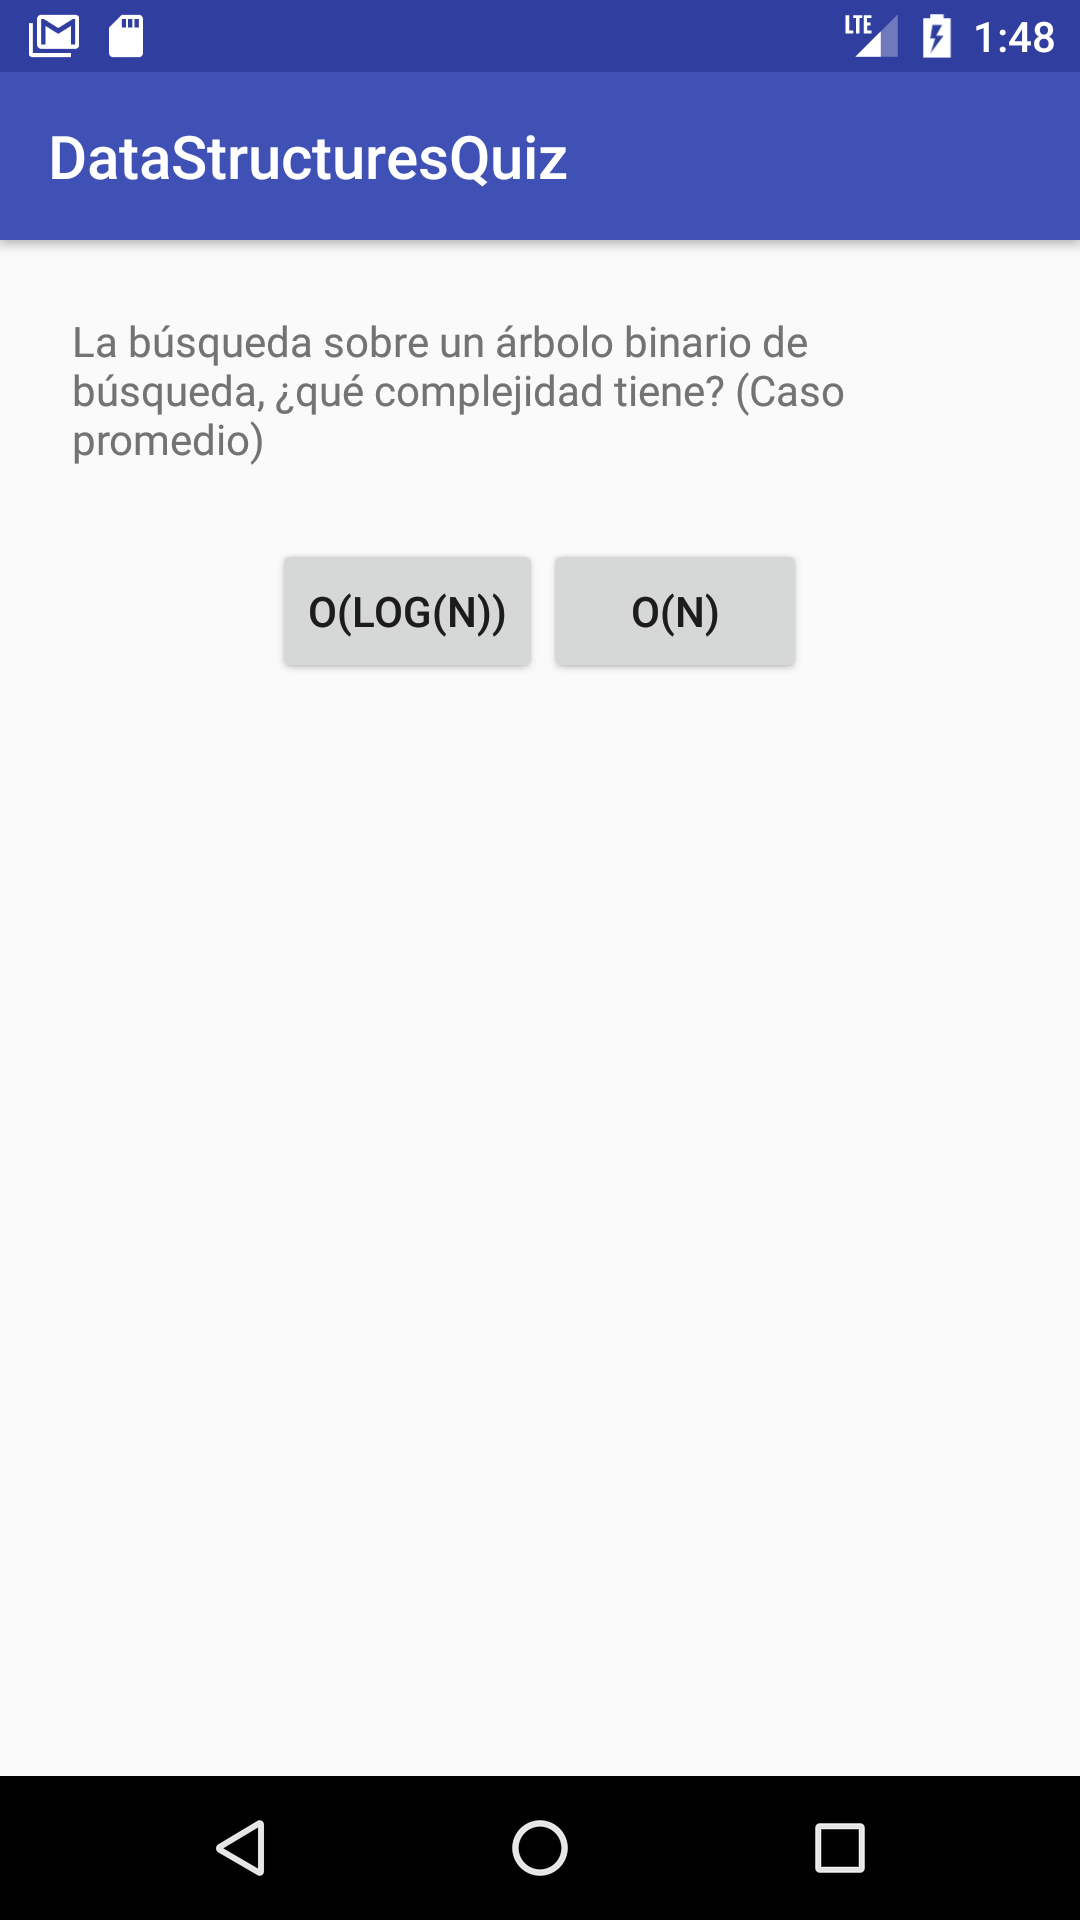
\includegraphics[scale=.1]{quiz_app}}%
    \qquad
    \subfloat[Se muestra el \texttt{Toast} con el mensaje después de dar clic sobre el prime botón]{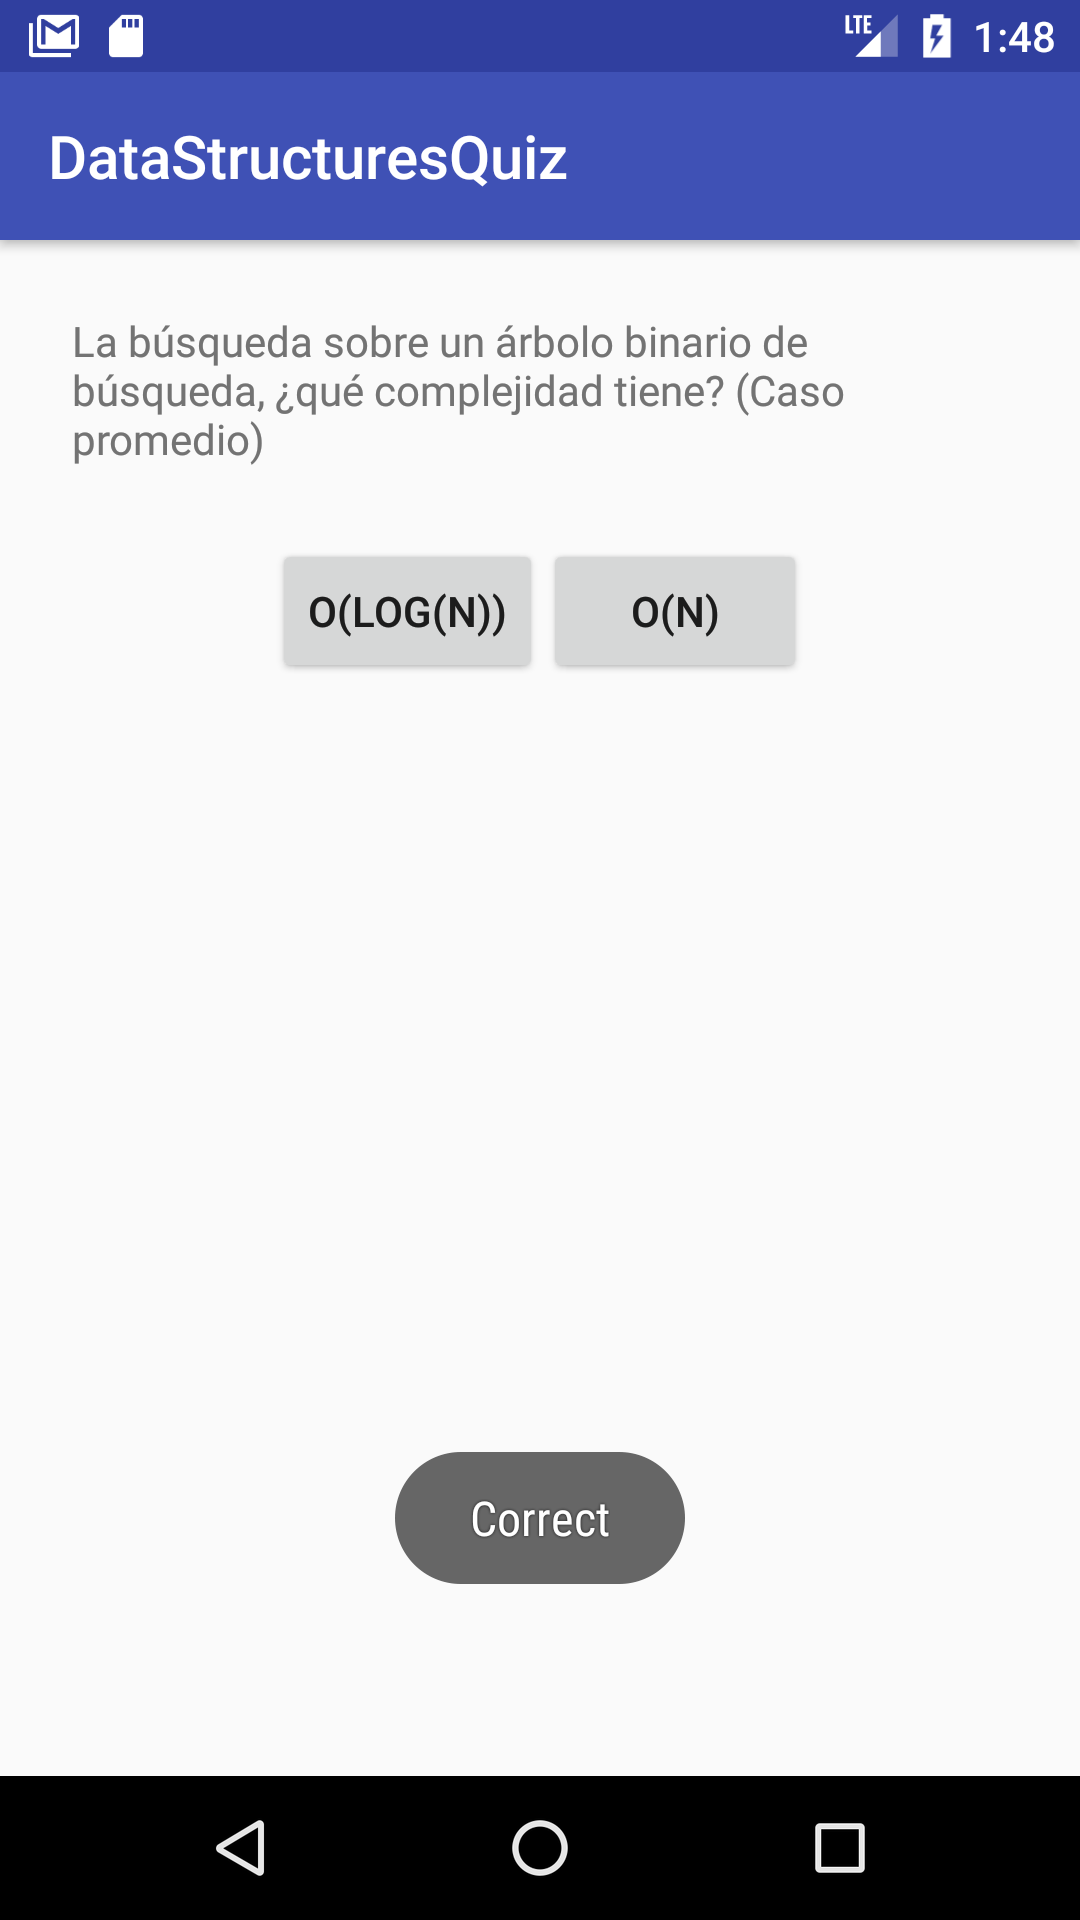
\includegraphics[scale=.1]{quiz_app_clicked} }%
    \caption{Capturas de la ejecución de la aplicación  Data Structures Quiz.}
    \label{fig:quiz_app}%
\end{figure}

\subsection*{SDK para Android de NAOqi}
\label{\detokenize{dev_docs:sdk-para-android-de-naoqi}}
Para ejecutar módulos de manera remota sobre los robots de NAOqi es necesario
contar con un SDK para la plataforma y el lenguaje con el que se desee
desarrollar. La plataforma en cuestión es Android, y Aldebaran brinda un SDK
de Java específicamente para este sistema. Como ya se mencionó en la sección
sobre \sphinxstylestrong{NAOqi}, el SDK de Java utiliza el \sphinxstylestrong{framework qi}.

El SDK provisto  no ha sido actualizado y en el archivo \sphinxstyleemphasis{.jar} no es compatible
con nuevas versiones de Android a partir de la 5.

El SDK se añade al proyecto como si fuera cualquier bibliotecas desarrollada
por un tercero. Cambiando la vista del proyecto que viene por defecto, \sphinxstyleemphasis{Android},
a \sphinxstyleemphasis{Project}, se puede copiar el archivo \sphinxcode{javanaoqi-sdk-2.1.4-android.jar}
al directorio en la ubicación \sphinxstyleemphasis{app/libs}. Después se configura el archivo
del gradle de la aplicación y del proyecto.


\subsubsection{Configuración de Gradle}
\label{\detokenize{dev_docs:configuracion-de-gradle}}
El sistema de construcción de Android Studio está basado en Gradle, y el plugin
de Android para Gradle adiciona varias características que están
construidas específicamente para aplicaciones de Android.\\

\begin{remark}
Gradle es un sistema de automatización de construcción de código abierto
enfocado a la flexibilidad y desempeño.
\end{remark}

La última versión del plugin de Gradle compatible con el SDK que brinda
Aldebaran es la 1.3.1. Por lo tanto después de sumar a nuestro directorio
\sphinxstyleemphasis{app/libs} se configura lo siguiente en el archivo \sphinxcode{buldgradle} del
proyecto:

\fvset{hllines={, ,}}%
\begin{sphinxVerbatim}[commandchars=\\\{\}]
\PYG{n+nx}{buildscript} \PYG{p}{\PYGZob{}}
  \PYG{n+nx}{dependencies} \PYG{p}{\PYGZob{}}
    \PYG{n+nx}{classpath} \PYG{l+s+s1}{\PYGZsq{}com.android.tools.build:gradle:1.3.1\PYGZsq{}}
  \PYG{p}{\PYGZcb{}}
\PYG{p}{\PYGZcb{}}
\end{sphinxVerbatim}

Por último sólo se agrega a las dependencias dentro del archivo \sphinxcode{buildgradle}
de la aplicación \sphinxcode{compilefiles('libs/java-naoqi-sdk-2.1.4-android.jar')}, que
compila el SDK de NAOqi.


\section*{ Firebase para Android}
\label{\detokenize{dev_docs:firebase-para-android}}

% \paragraph{Añadir Firebase a un proyecto de Android}
% \label{\detokenize{dev_docs:anadir-firebase-a-un-proyecto-de-android}}

Los servicios de Firebase utilizados son Firebase Realtime Database
y Authentication. Este último a través de la biblioteca Firebase UI.

Antes de poder utilizar Firebase en una aplicación se debe agregar Firebase a ésta. Después de crear un proyecto en la consola 
de Firebase se siguen los pasos que ésta nos muestra
para añadir Firebase a nuestras aplicaciones ya sea web 
o móviles, en nuestro caso para dispositivos Android.
La consola genera un archivo de configuración
que se añade a la aplicación y luego
se agrega el SDK para poder utilizar las bibliotecas de Firebase en el proyecto.

Cada biblioteca de Firebase que se desee utilizar se añade a las dependencias.
Por ejemplo, sumando a las dependencias de Gradle  \sphinxcode{com.google.firebase:firebase-\\database:11.6.2}
se tiene acceso a a la base de datos en tiempo real que provee Firebase.


\subsection*{Firebase Realtime Database}
\label{\detokenize{dev_docs:firebase-realtime-database}}
Para comenzar a usar la Firebase Realtime Database en la aplicación,
se debe sumar a las dependencias del archivo \sphinxcode{buildgradle}, de la aplicación,
\sphinxcode{'compile.com.google.firebase:firebase-database:11.8.0'}.

%Los datos de Firebase se escriben en una referencia de \sphinxcode{FirebaseDatabase};
%para recuperarlos, se debe adjuntar un agente de escucha o escuchador asíncrono a la
%referencia. El agente de escucha se activa una vez para el estado inicial de los
%datos y otra vez cuando los datos cambian.

%
%\subparagraph{Obtener una DatabaseReference}
%\label{\detokenize{dev_docs:obtener-una-databasereference}}

Para leer y escribir en la base de datos, necesitas una instancia de
\texttt{DatabaseReference}:

\fvset{hllines={, ,}}%
\begin{sphinxVerbatim}[commandchars=\\\{\}]
\PYG{k+kd}{private} \PYG{n}{DatabaseReference} \PYG{n}{mDatabase}\PYG{o}{;}
\PYG{n}{mDatabase} \PYG{o}{=} \PYG{n}{FirebaseDatabase}\PYG{o}{.}\PYG{n+na}{getInstance}\PYG{o}{(}\PYG{o}{)}\PYG{o}{.}\PYG{n+na}{getReference}\PYG{o}{(}\PYG{o}{)}\PYG{o}{;}
\end{sphinxVerbatim}


\subsubsection{Leer y escribir datos}
\label{\detokenize{dev_docs:leer-y-escribir-datos}}
Para ejecutar una escritura básica se usa \sphinxcode{setValue()} para guardar datos en
una referencia que se especifique.

Los tipos de datos que se pueden almacenar son los siguientes:
\begin{itemize}
\item {}
\texttt{String}

\item {}
\texttt{Long}

\item {}
\texttt{Double}

\item {}
\texttt{Boolean}

\item {}
\texttt{Map\textless{}String, Object\textgreater{}}

\item {}
\texttt{List\textless{}Object\textgreater{}}

\end{itemize}

También se puede pasar un objeto personalizado de Java con la restricción
de que la definición de la clase debe tener un constructor predeterminado
que no recibe parámetros y tiene métodos públicos para obtener a los atributos
del objeto.

El siguiente fragmento muestra como escribir un nuevo usuario en la base de
datos.

\fvset{hllines={, ,}}%
\begin{sphinxVerbatim}[commandchars=\\\{\}]
\PYG{k+kd}{public} \PYG{k+kt}{void} \PYG{n+nf}{saveUserToDatabase}\PYG{o}{(}\PYG{n}{String} \PYG{n}{uid}\PYG{o}{,} \PYG{n}{String} \PYG{n}{email}\PYG{o}{)} \PYG{o}{\PYGZob{}}
  \PYG{n}{mDatabase}\PYG{o}{.}\PYG{n+na}{child}\PYG{o}{(}\PYG{l+s}{\PYGZdq{}users/\PYGZdq{}} \PYG{o}{+} \PYG{n}{uid}\PYG{o}{)}\PYG{o}{.}\PYG{n+na}{setValue}\PYG{o}{(}\PYG{n}{email}\PYG{o}{)}\PYG{o}{;}
\PYG{o}{\PYGZcb{}}
\end{sphinxVerbatim}


\subsubsection{Detección de eventos en valores}
\label{\detokenize{dev_docs:detecteccion-eventos-de-valores}}
Para leer datos en una ruta de acceso y escuchar actualizaciones, usa el
método \sphinxcode{addValueEventListener()} o el método \sphinxcode{addListenerForSingleValueEvent()}
para agregar un \sphinxcode{ValueEventListener} a un objetos \sphinxcode{DatabaseReference}.

Un escuchador \sphinxcode{ValueEventListener} de una referencia de la base de datos
tiene una método callback \sphinxcode{onDataChange()} que obtiene una captura estática
del contiene en la ruta determinada.

El ejemplo siguiente es parte de una aplicación que muestra mensajes
almacenados en la base de datos:

\fvset{hllines={, ,}}%
\begin{sphinxVerbatim}[commandchars=\\\{\}]
\PYG{n}{mMessagesReference}\PYG{o}{.}\PYG{n+na}{addValueEventListener}\PYG{o}{(}\PYG{k}{new} \PYG{n}{ValueEventListener}\PYG{o}{(}\PYG{o}{)}\PYG{o}{\PYGZob{}}
  \PYG{n+nd}{@Override}
  \PYG{k+kd}{public} \PYG{k+kt}{void} \PYG{n+nf}{onDataChange}\PYG{o}{(}\PYG{n}{DataSnapshot} \PYG{n}{snapshot}\PYG{o}{)} \PYG{o}{\PYGZob{}}
    \PYG{n}{Message} \PYG{n}{msg} \PYG{o}{=} \PYG{n}{snapshot}\PYG{o}{.}\PYG{n+na}{getValue}\PYG{o}{(}\PYG{n}{Message}\PYG{o}{.}\PYG{n+na}{class}\PYG{o}{)}\PYG{o}{;}
    \PYG{c+c1}{//...}
  \PYG{o}{\PYGZcb{}}
\PYG{o}{\PYGZcb{}}\PYG{o}{)}
\end{sphinxVerbatim}

El escuchador recibe un objeto \sphinxcode{DataSnapshot} que contiene los datos de la
ubicación especifica al momentos del evento.

La diferencia entre \sphinxcode{addValueEventListener()} y
\sphinxcode{addListenerForSingleValue\\Event()} es que el primero se suscribe a cierta
ubicación para escuchar cambios, y el segundo lee los datos de una ubicación
una sola vez.


\subsubsection{Actualización o borrado de datos}
\label{\detokenize{dev_docs:actulizacion-o-borrado-de-datos}}
Para actualizar se llama al método \sphinxcode{update\\Children()} y para eliminar datos
en una referencia se usa \sphinxcode{removeValue} o se pasa como parámetro un valor
\sphinxcode{null} a \sphinxcode{setValue()}.

También existe el método \sphinxcode{push()} para añadir una entrada con un identificador
único sobre una referencia.


\subsection*{Firebase UI Authentication}
\label{\detokenize{dev_docs:firebase-ui-authentication}}
%FirebaseUI es una biblioteca de código abierto que ofrece referencias a la IU
%de manera simple y personalizable, sobre los SDK de Firebase, para eliminar
%código repetitivo y promover mejores prácticas (en cuanto a la experiencia
%de usuario y seguridad) para la autenticación.

Es una API para manejar el flujo del inicio de sesión con una
dirección de correo electrónico, números de teléfono, y a través de
proveedores como Google Sign-In, y Facebook Login. Está construido sobre
Firebase Authentication.

%FirebaseUI se integra con \sphinxstylestrong{Smart Lock} para guardar y recuperar credenciales,
%habilita el inicio de sesión con un solo click en una aplicación cuando el
%usuario regresa a esta. Maneja casos de uso complicados como la recuperación
%de la cuenta y el enlace con la cuenta que son inseguros y difíciles de implementar
%usando la API base de Firebase Authentication.


\subsubsection{Configuración}
\label{\detokenize{dev_docs:configuracion}}
Como prerrequisito, la aplicación debe estar configurada para utilizar Firebase.
Después, se agrega a la biblioteca de FirebaseUI auth en las dependencias de
\sphinxcode{buildgradle} de la aplicación.

\fvset{hllines={, ,}}%
\begin{sphinxVerbatim}[commandchars=\\\{\}]
\PYG{n+nx}{dependencies} \PYG{p}{\PYGZob{}}
  \PYG{n+nx}{compile} \PYG{l+s+s1}{\PYGZsq{}com.firebaseui:firebase\PYGZhy{}ui\PYGZhy{}auth:3.0.0\PYGZsq{}}
\PYG{p}{\PYGZcb{}}
\end{sphinxVerbatim}


\subsubsection{Uso de FirebaseUI para autenticación}
\label{\detokenize{dev_docs:uso-de-firebaseui-para-autenticacion}}
Antes de llamar al flujo de autenticación de FirebaseUI, la aplicación debe
checar que un usuario ya esté registrado de una sesión previa. Este caso
es cuando el usuario inicio sesión y salió de la aplicación para luego regresar
a esta.

\fvset{hllines={, ,}}%
\begin{sphinxVerbatim}[commandchars=\\\{\}]
\PYG{n}{FirebaseAuth} \PYG{n}{auth} \PYG{o}{=} \PYG{n}{FirebaseAuth}\PYG{o}{.}\PYG{n+na}{getInstance}\PYG{o}{(}\PYG{o}{)}\PYG{o}{;}
\PYG{k}{if} \PYG{o}{(}\PYG{n}{auth}\PYG{o}{.}\PYG{n+na}{getCurrentUser}\PYG{o}{(}\PYG{o}{)} \PYG{o}{!}\PYG{o}{=} \PYG{k+kc}{null}\PYG{o}{)} \PYG{o}{\PYGZob{}}
  \PYG{c+c1}{// el usuario tiene abierta la sesión}
\PYG{o}{\PYGZcb{}} \PYG{k}{else} \PYG{o}{\PYGZob{}}
  \PYG{c+c1}{// el usuario no ha iniciado sesión}
\PYG{o}{\PYGZcb{}}
\end{sphinxVerbatim}

El punto de entrada para el flujo de la autenticación es la clase
\sphinxcode{com.firebase.ui.auth.AuthUI}.


\subsubsection{Inicio de sesión}
\label{\detokenize{dev_docs:inicio-de-sesion}}
Si un usuario no ha iniciado sesión, entonces el proceso de inicio de sesión
puede empezar creando un intent sign-in usando \sphinxcode{AuthUISignInIntent\\Builder}.
Se puede recuperar una instancia del constructor llamando
\sphinxcode{createSignIn\\IntentBuilder()} en la instancia retomada de AuthUI.

El constructor provee las siguientes opciones de personalización para el flujo
de la autenticación:
\begin{itemize}
\item {} 
El conjunto de proveedores de autenticación puede especificarse (Google, Twitter, Facebook)

\item {} 
Un URL con los términos de servicio para la aplicación.

\item {} 
Un tema personalizado puede ser especificado para el flujo, el cual se aplica a todas las actividades en el flujo para que haya consistencia de colores y tipografía.

\end{itemize}

Si no se requiere personalizar , y solo se necesita el correo electrónico para
autenticarse, el flujo del inicio de sesión comienza como sigue:

\fvset{hllines={, ,}}%
\begin{sphinxVerbatim}[commandchars=\\\{\}]
\PYG{c+c1}{// Un valor para el código de petición arbitrario}
\PYG{k+kd}{private} \PYG{k+kd}{static} \PYG{k+kd}{final} \PYG{k+kt}{int} \PYG{n}{RC\PYGZus{}SIGN\PYGZus{}IN} \PYG{o}{=} \PYG{l+m+mi}{123}\PYG{o}{;}

\PYG{c+c1}{// ...}

\PYG{n}{startActivityForResult}\PYG{o}{(}
  \PYG{c+c1}{// obtiene una instancia de AuthUI basado en la aplicación por defecto}
  \PYG{n}{AuthUI}\PYG{o}{.}\PYG{n+na}{getInstance}\PYG{o}{(}\PYG{o}{)}\PYG{o}{.}\PYG{n+na}{createSignInIntentBuilder}\PYG{o}{(}\PYG{o}{)}\PYG{o}{.}\PYG{n+na}{build}\PYG{o}{(}\PYG{o}{)}\PYG{o}{,}
  \PYG{n}{RC\PYGZus{}SIGN\PYGZus{}IN}\PYG{o}{)}\PYG{o}{;}
\end{sphinxVerbatim}

El segundo parámetro de \sphinxcode{startActivityForResult()} (\sphinxcode{RC\_SIGN\_IN})  es un
código de petición para identificar la petición cuando el resultado retorna
a la aplicación en el métodos \sphinxcode{onActivityResult()}.

El flujo de la autenticación suministra varios códigos de respuesta, entre
los más comunes están:
\begin{itemize}
\item {} 
\sphinxcode{Activity.RESULT\_OK}, si es el usuario inició sesión.

\item {} 
\sphinxcode{Activity.RESULT\_CANCELLED}, si el usuario canceló manualmente el inicio de sesión.

\item {} 
\sphinxcode{ErrorCodes.NO\_NETWORK}, si no hay conexión a una red.

\item {} 
\sphinxcode{ErrorCodes.UNKNOWN\_ERROR},  todos los otros errores.

\end{itemize}

Siguiendo con el ejemplo del inicio de sesión con el correo electrónico,
el método \sphinxcode{onActivityResult()} queda como sigue:

\fvset{hllines={, ,}}%
\begin{sphinxVerbatim}[commandchars=\\\{\}]
\PYG{k+kd}{protected} \PYG{k+kt}{void} \PYG{n+nf}{onActivityResult}\PYG{o}{(}\PYG{k+kt}{int} \PYG{n}{requestCode}\PYG{o}{,} \PYG{k+kt}{int} \PYG{n}{resultCode}\PYG{o}{,} \PYG{n}{Intent} \PYG{n}{data}\PYG{o}{)} \PYG{o}{\PYGZob{}}
    \PYG{k+kd}{super}\PYG{o}{.}\PYG{n+na}{onActivityResult}\PYG{o}{(}\PYG{n}{requestCode}\PYG{o}{,} \PYG{n}{resultCode}\PYG{o}{,} \PYG{n}{data}\PYG{o}{)}\PYG{o}{;}
    \PYG{c+c1}{// RC\PYGZus{}SIGN\PYGZus{}IN es el segundo parámetro que se pasó a startActivityForResult}
    \PYG{k}{if} \PYG{o}{(}\PYG{n}{requestCode} \PYG{o}{=}\PYG{o}{=} \PYG{n}{RC\PYGZus{}SIGN\PYGZus{}IN}\PYG{o}{)} \PYG{o}{\PYGZob{}}
        \PYG{n}{IdpResponse} \PYG{n}{response} \PYG{o}{=} \PYG{n}{IdpResponse}\PYG{o}{.}\PYG{n+na}{fromResultIntent}\PYG{o}{(}\PYG{n}{data}\PYG{o}{)}\PYG{o}{;}

        \PYG{c+c1}{// Si el usuario inició sesión exitosamente}
        \PYG{k}{if} \PYG{o}{(}\PYG{n}{resultCode} \PYG{o}{=}\PYG{o}{=} \PYG{n}{RESULT\PYGZus{}OK}\PYG{o}{)} \PYG{o}{\PYGZob{}}
            \PYG{n}{startActivity}\PYG{o}{(}\PYG{n}{SignedInActivity}\PYG{o}{.}\PYG{n+na}{createIntent}\PYG{o}{(}\PYG{k}{this}\PYG{o}{,} \PYG{n}{response}\PYG{o}{)}\PYG{o}{)}\PYG{o}{;}
            \PYG{n}{finish}\PYG{o}{(}\PYG{o}{)}\PYG{o}{;}
        \PYG{o}{\PYGZcb{}} \PYG{k}{else} \PYG{o}{\PYGZob{}}
            \PYG{c+c1}{// El inicio de sesión falló}
            \PYG{k}{if} \PYG{o}{(}\PYG{n}{response} \PYG{o}{=}\PYG{o}{=} \PYG{k+kc}{null}\PYG{o}{)} \PYG{o}{\PYGZob{}}
                \PYG{c+c1}{// El usuario presión el botón de regresar}
                \PYG{n}{showSnackbar}\PYG{o}{(}\PYG{n}{R}\PYG{o}{.}\PYG{n+na}{string}\PYG{o}{.}\PYG{n+na}{sign\PYGZus{}in\PYGZus{}cancelled}\PYG{o}{)}\PYG{o}{;}
                \PYG{k}{return}\PYG{o}{;}
            \PYG{o}{\PYGZcb{}}

            \PYG{k}{if} \PYG{o}{(}\PYG{n}{response}\PYG{o}{.}\PYG{n+na}{getError}\PYG{o}{(}\PYG{o}{)}\PYG{o}{.}\PYG{n+na}{getErrorCode}\PYG{o}{(}\PYG{o}{)} \PYG{o}{=}\PYG{o}{=} \PYG{n}{ErrorCodes}\PYG{o}{.}\PYG{n+na}{NO\PYGZus{}NETWORK}\PYG{o}{)} \PYG{o}{\PYGZob{}}
                \PYG{n}{showSnackbar}\PYG{o}{(}\PYG{n}{R}\PYG{o}{.}\PYG{n+na}{string}\PYG{o}{.}\PYG{n+na}{no\PYGZus{}internet\PYGZus{}connection}\PYG{o}{)}\PYG{o}{;}
                \PYG{k}{return}\PYG{o}{;}
            \PYG{o}{\PYGZcb{}}
            \PYG{n}{showSnackbar}\PYG{o}{(}\PYG{n}{R}\PYG{o}{.}\PYG{n+na}{string}\PYG{o}{.}\PYG{n+na}{unknown\PYGZus{}error}\PYG{o}{)}\PYG{o}{;}
            \PYG{n}{Log}\PYG{o}{.}\PYG{n+na}{e}\PYG{o}{(}\PYG{n}{TAG}\PYG{o}{,} \PYG{l+s}{\PYGZdq{}Sign\PYGZhy{}in error: \PYGZdq{}}\PYG{o}{,} \PYG{n}{response}\PYG{o}{.}\PYG{n+na}{getError}\PYG{o}{(}\PYG{o}{)}\PYG{o}{)}\PYG{o}{;}
        \PYG{o}{\PYGZcb{}}
    \PYG{o}{\PYGZcb{}}
\PYG{o}{\PYGZcb{}}
\end{sphinxVerbatim}


\subsubsection{Cierre de sesión}
\label{\detokenize{dev_docs:cierre-de-sesion}}
AuthUI brinda un método \sphinxcode{signOut} simple que encapsula todo el proceso
que conlleva un cierre de sesión. El método retornar una objeto \sphinxcode{Task}
que se marca completamente una vez que todo el proceso de cierre de sesión
se ha completado.

\fvset{hllines={, ,}}%
\begin{sphinxVerbatim}[commandchars=\\\{\}]
\PYG{k+kd}{public} \PYG{k+kt}{void} \PYG{n+nf}{signOut}\PYG{o}{(}\PYG{o}{)}\PYG{o}{\PYGZob{}}
    \PYG{n}{AuthUI}\PYG{o}{.}\PYG{n+na}{getInstance}\PYG{o}{(}\PYG{o}{)}\PYG{o}{.}\PYG{n+na}{signOut}\PYG{o}{(}\PYG{k}{this}\PYG{o}{)}
            \PYG{o}{.}\PYG{n+na}{addOnCompleteListener}\PYG{o}{(}\PYG{k}{new} \PYG{n}{OnCompleteListener}\PYG{o}{\PYGZlt{}}\PYG{n}{Void}\PYG{o}{\PYGZgt{}}\PYG{o}{(}\PYG{o}{)} \PYG{o}{\PYGZob{}}
                \PYG{n+nd}{@Override}
                \PYG{k+kd}{public} \PYG{k+kt}{void} \PYG{n+nf}{onComplete}\PYG{o}{(}\PYG{n+nd}{@NonNull} \PYG{n}{Task}\PYG{o}{\PYGZlt{}}\PYG{n}{Void}\PYG{o}{\PYGZgt{}} \PYG{n}{task}\PYG{o}{)} \PYG{o}{\PYGZob{}}
                    \PYG{k}{if} \PYG{o}{(}\PYG{n}{task}\PYG{o}{.}\PYG{n+na}{isSuccessful}\PYG{o}{(}\PYG{o}{)}\PYG{o}{)} \PYG{o}{\PYGZob{}}
                        \PYG{n}{startActivity}\PYG{o}{(}\PYG{n}{MyActivity}\PYG{o}{.}\PYG{n+na}{createIntent}\PYG{o}{(}\PYG{n}{SignInActivity}\PYG{o}{.}\PYG{n+na}{this}\PYG{o}{)}\PYG{o}{)}\PYG{o}{;}
                        \PYG{n}{finish}\PYG{o}{(}\PYG{o}{)}\PYG{o}{;}
                    \PYG{o}{\PYGZcb{}} \PYG{k}{else} \PYG{o}{\PYGZob{}}
                        \PYG{c+c1}{// Falló el cierre de sesión}
                    \PYG{o}{\PYGZcb{}}
                \PYG{o}{\PYGZcb{}}
            \PYG{o}{\PYGZcb{}}\PYG{o}{)}\PYG{o}{;}
\PYG{o}{\PYGZcb{}}
\end{sphinxVerbatim}


\section*{ ButterKnife}
\label{\detokenize{dev_docs:butterknife}}
ButterKnife es una biblioteca de viewbinding, esto quiere decir que genera
objetos view a partir de recursos, pero lo que la hace especial es que evita
el código repetitivo, como llamar a la función \sphinxcode{findViewById}. ButterKnife
ayuda a enlazar atributos, métodos y views.


\subsection*{Configuración}
\label{\detokenize{dev_docs:id1}}
Para comenzar a utilizar butterknife en un proyecto. Solo se agrega a Las
dependencias del \sphinxcode{buildgradle} lo siguiente:

\fvset{hllines={, ,}}%
\begin{sphinxVerbatim}[commandchars=\\\{\}]
\PYG{n+nx}{compile} \PYG{l+s+s1}{\PYGZsq{}com.jakewharton:butterknife:8.8.1\PYGZsq{}}
\PYG{n+nx}{provided} \PYG{l+s+s1}{\PYGZsq{}com.jakewharton:butterknife\PYGZhy{}compiler:8.8.1\PYGZsq{}}
\end{sphinxVerbatim}


\subsection*{Uso}
\label{\detokenize{dev_docs:uso}}
Para entender mejor las características que tiene ButterKnife supongamos que
tenemos una actividad con un botón que reaccione a clics. Sin usar ButterKnife
la actividad queda como sigue:

\fvset{hllines={, ,}}%
\begin{sphinxVerbatim}[commandchars=\\\{\}]
\PYG{k+kd}{public} \PYG{k+kd}{class} \PYG{n+nc}{MainActivity} \PYG{k+kd}{extends} \PYG{n}{AppCompatActivity} \PYG{o}{\PYGZob{}}
  \PYG{k+kd}{private} \PYG{n}{TextView} \PYG{n}{mTextView}\PYG{o}{;}
  \PYG{k+kd}{private} \PYG{n}{Button} \PYG{n}{mButton}\PYG{o}{;}

  \PYG{n+nd}{@Override}
  \PYG{k+kd}{protected} \PYG{k+kt}{void} \PYG{n+nf}{onCreate}\PYG{o}{(}\PYG{n}{Bundle} \PYG{n}{savedInstanceState}\PYG{o}{)} \PYG{o}{\PYGZob{}}
      \PYG{k+kd}{super}\PYG{o}{.}\PYG{n+na}{onCreate}\PYG{o}{(}\PYG{n}{savedInstanceState}\PYG{o}{)}\PYG{o}{;}
      \PYG{n}{setContentView}\PYG{o}{(}\PYG{n}{R}\PYG{o}{.}\PYG{n+na}{layout}\PYG{o}{.}\PYG{n+na}{activity\PYGZus{}main}\PYG{o}{)}\PYG{o}{;}

      \PYG{n}{mButton} \PYG{o}{=} \PYG{o}{(}\PYG{n}{Button}\PYG{o}{)} \PYG{n}{findViewById}\PYG{o}{(}\PYG{n}{R}\PYG{o}{.}\PYG{n+na}{id}\PYG{o}{.}\PYG{n+na}{AButton}\PYG{o}{)}\PYG{o}{;}
      \PYG{n}{mTextView} \PYG{o}{=} \PYG{o}{(}\PYG{n}{TextView}\PYG{o}{)} \PYG{n}{findViewById}\PYG{o}{(}\PYG{n}{R}\PYG{o}{.}\PYG{n+na}{id}\PYG{o}{.}\PYG{n+na}{texView}\PYG{o}{)}\PYG{o}{;}

      \PYG{n}{mAOptionButton}\PYG{o}{.}\PYG{n+na}{setOnClickListener}\PYG{o}{(}\PYG{k}{new} \PYG{n}{View}\PYG{o}{.}\PYG{n+na}{OnClickListener}\PYG{o}{(}\PYG{o}{)} \PYG{o}{\PYGZob{}}
          \PYG{n+nd}{@Override}
          \PYG{k+kd}{public} \PYG{k+kt}{void} \PYG{n+nf}{onClick}\PYG{o}{(}\PYG{n}{View} \PYG{n}{view}\PYG{o}{)} \PYG{o}{\PYGZob{}}
           \PYG{c+c1}{// Haz algo}
          \PYG{o}{\PYGZcb{}}
      \PYG{o}{\PYGZcb{}}\PYG{o}{)}\PYG{o}{;}
    \PYG{o}{\PYGZcb{}}
  \PYG{o}{\PYGZcb{}}
\end{sphinxVerbatim}

Utilizando ButterKnife la actividad cambiaría a los siguiente:

\fvset{hllines={, ,}}%
\begin{sphinxVerbatim}[commandchars=\\\{\}]
\PYG{k+kd}{public} \PYG{k+kd}{class} \PYG{n+nc}{MainActivity} \PYG{k+kd}{extends} \PYG{n}{AppCompatActivity} \PYG{o}{\PYGZob{}}
  \PYG{n+nd}{@BindView}\PYG{o}{(}\PYG{n}{R}\PYG{o}{.}\PYG{n+na}{id}\PYG{o}{.}\PYG{n+na}{textView}\PYG{o}{)}
  \PYG{n}{TextView} \PYG{n}{mTextView}\PYG{o}{;}

  \PYG{n+nd}{@Override}
  \PYG{k+kd}{protected} \PYG{k+kt}{void} \PYG{n+nf}{onCreate}\PYG{o}{(}\PYG{n}{Bundle} \PYG{n}{savedInstanceState}\PYG{o}{)} \PYG{o}{\PYGZob{}}
      \PYG{k+kd}{super}\PYG{o}{.}\PYG{n+na}{onCreate}\PYG{o}{(}\PYG{n}{savedInstanceState}\PYG{o}{)}\PYG{o}{;}
      \PYG{n}{setContentView}\PYG{o}{(}\PYG{n}{R}\PYG{o}{.}\PYG{n+na}{layout}\PYG{o}{.}\PYG{n+na}{activity\PYGZus{}main}\PYG{o}{)}\PYG{o}{;}
      \PYG{c+c1}{// Enlaza butterknife a la actividad}
      \PYG{n}{ButterKnife}\PYG{o}{.}\PYG{n+na}{bind}\PYG{o}{(}\PYG{k}{this}\PYG{o}{)}\PYG{o}{;}
  \PYG{o}{\PYGZcb{}}

  \PYG{n+nd}{@OnClick}\PYG{o}{(}\PYG{n}{R}\PYG{o}{.}\PYG{n+na}{id}\PYG{o}{.}\PYG{n+na}{AButton}\PYG{o}{)}
  \PYG{k+kd}{public} \PYG{k+kt}{void} \PYG{n+nf}{OnClickMyButton}\PYG{o}{(}\PYG{o}{)} \PYG{o}{\PYGZob{}}
    \PYG{c+c1}{// Haz algo}
  \PYG{o}{\PYGZcb{}}

\PYG{o}{\PYGZcb{}}
\end{sphinxVerbatim}

Al comparar se nota como evita duplicar código, y el código de los escuchadores
es mucho más simple y parece explicarse por sí mismo.


\section*{ Volley}
\label{\detokenize{dev_docs:volley}}
Volley es una biblioteca HTTP que facilita el acceso a la red en aplicaciones
de Android. Algunos de sus beneficios son los siguientes:
\begin{itemize}
\item {} 
Programación automática de peticiones a través de la red.

\item {} 
Múltiples conexiones concurrentes.

\item {} 
Soporte para priorizar peticiones.

\item {} 
Una API para cancelar peticiones.

\item {} 
Personalizable, por ejemplo, se puede añadir la opción de reintentar un petición.

\end{itemize}


\subsection*{Configuración}
\label{\detokenize{dev_docs:id2}}
La manera más sencilla de añadir Volley a un proyecto es a través de la dependencia
en el \sphinxcode{buildgradle} de la aplicación.

\fvset{hllines={, ,}}%
\begin{sphinxVerbatim}[commandchars=\\\{\}]
\PYG{n+nx}{dependencies} \PYG{p}{\PYGZob{}}
\PYG{p}{...}
\PYG{n+nx}{compile} \PYG{l+s+s1}{\PYGZsq{}com.android.volley:volley:1.1.0\PYGZsq{}}
\PYG{p}{\PYGZcb{}}
\end{sphinxVerbatim}


\subsection*{Enviando una petición simple}
\label{\detokenize{dev_docs:enviando-una-peticion-simple}}
A un alto nivel, se utiliza Volley creando un objeto \sphinxcode{RequestQueue} y
pasándole objetos \sphinxcode{Request}. \sphinxcode{RequestQueue} administra hilos trabajadores
para ejecutar operaciones en red, leyendo y escribiendo desde el caché, y
parseando respuestas. Las peticiones hacen el parseo de respuestas en crudo
y Volley se ocupa de remitir la respuesta parseada de regreso al hilo principal
para su entrega.

Volley provee una método \sphinxcode{VolleynewRequestQueue} que prepara una
\sphinxcode{RequestQueue}, usando valores por defecto, e inicia la cola. El
siguiente ejemplo presenta cómo se crea una nueva cola de peticiones,
así como una simple petición \sphinxcode{GET} a \sphinxcode{www.google.com}, recibiendo  la respuesta
en una cadena y mostrándola en un \sphinxcode{TextView}.

\fvset{hllines={, ,}}%
\begin{sphinxVerbatim}[commandchars=\\\{\}]
\PYG{n+nd}{@BindView}\PYG{o}{(}\PYG{n}{R}\PYG{o}{.}\PYG{n+na}{id}\PYG{o}{.}\PYG{n+na}{text}\PYG{o}{)}
\PYG{n}{TextView} \PYG{n}{mTextView}\PYG{o}{;}

\PYG{c+c1}{// Instancia a la cola de peticiones}
\PYG{n}{RequestQueue} \PYG{n}{queue} \PYG{o}{=} \PYG{n}{Volley}\PYG{o}{.}\PYG{n+na}{newRequestQueue}\PYG{o}{(}\PYG{k}{this}\PYG{o}{)}\PYG{o}{;}
\PYG{n}{String} \PYG{n}{url} \PYG{o}{=}\PYG{l+s}{\PYGZdq{}http://www.google.com\PYGZdq{}}\PYG{o}{;}

\PYG{c+c1}{// Solicita una respuesta en formato de cadena haciendo un GET al URL}
\PYG{n}{StringRequest} \PYG{n}{stringRequest} \PYG{o}{=} \PYG{k}{new} \PYG{n}{StringRequest}\PYG{o}{(}\PYG{n}{Request}\PYG{o}{.}\PYG{n+na}{Method}\PYG{o}{.}\PYG{n+na}{GET}\PYG{o}{,} \PYG{n}{url}\PYG{o}{,}
          \PYG{k}{new} \PYG{n}{Response}\PYG{o}{.}\PYG{n+na}{Listener}\PYG{o}{\PYGZlt{}}\PYG{n}{String}\PYG{o}{\PYGZgt{}}\PYG{o}{(}\PYG{o}{)} \PYG{o}{\PYGZob{}}
  \PYG{n+nd}{@Override}
  \PYG{k+kd}{public} \PYG{k+kt}{void} \PYG{n+nf}{onResponse}\PYG{o}{(}\PYG{n}{String} \PYG{n}{response}\PYG{o}{)} \PYG{o}{\PYGZob{}}
      \PYG{n}{mTextView}\PYG{o}{.}\PYG{n+na}{setText}\PYG{o}{(}\PYG{l+s}{\PYGZdq{}Response is: \PYGZdq{}}\PYG{o}{+} \PYG{n}{response}\PYG{o}{.}\PYG{n+na}{substring}\PYG{o}{(}\PYG{l+m+mi}{0}\PYG{o}{,}\PYG{l+m+mi}{500}\PYG{o}{)}\PYG{o}{)}\PYG{o}{;}
  \PYG{o}{\PYGZcb{}}
\PYG{o}{\PYGZcb{}}\PYG{o}{,} \PYG{k}{new} \PYG{n}{Response}\PYG{o}{.}\PYG{n+na}{ErrorListener}\PYG{o}{(}\PYG{o}{)} \PYG{o}{\PYGZob{}}
  \PYG{n+nd}{@Override}
  \PYG{k+kd}{public} \PYG{k+kt}{void} \PYG{n+nf}{onErrorResponse}\PYG{o}{(}\PYG{n}{VolleyError} \PYG{n}{error}\PYG{o}{)} \PYG{o}{\PYGZob{}}
      \PYG{n}{mTextView}\PYG{o}{.}\PYG{n+na}{setText}\PYG{o}{(}\PYG{l+s}{\PYGZdq{}That didn\PYGZsq{}t work!\PYGZdq{}}\PYG{o}{)}\PYG{o}{;}
  \PYG{o}{\PYGZcb{}}
\PYG{o}{\PYGZcb{}}\PYG{o}{)}\PYG{o}{;}
\PYG{c+c1}{// Añade la petición a la cola RequestQueue}
\PYG{n}{queue}\PYG{o}{.}\PYG{n+na}{add}\PYG{o}{(}\PYG{n}{stringRequest}\PYG{o}{)}\PYG{o}{;}
\end{sphinxVerbatim}

Volley siempre entrega respuestas parseadas sobre el hilo principal. Ejecutarlo
sobre el hilo principal es conveniente para poblar elementos de la interfaz de
usuario con los datos recibidos.

\chapter{Herramientas para el desarrollo de la aplicación web\label{anexo:app-web}}


\section*{React}


React es una biblioteca de Javascript para crear interfaces de usuario
lanzada por Facebook en 2013.
Tiene tres características que la definen y distinguen  de otras
biblioteca o frameworks y son:
\begin{itemize}
\item {} 
Es \textbf{declarativa}, ya que permite crear interfaces de manera sencilla. Sólo se diseña una vista para cada estado de la aplicación; React actualizará de manera eficiente y \sphinxstylestrong{rederizará} los componentes correctos cuando los datos cambian.

\item {} 
Está \sphinxstylestrong{basado en componentes}, construye componentes encapsulados que manejan su propio estado, después se integran con otros para hacer IU más complejas.

\item {} 
React puede \sphinxstyleemphasis{renderizar} sobre un servidor usando node o en dispositivos móviles con React Native.

\end{itemize}


Los \textit{componentes} dividen la IU en piezas independientes y reutilizables; además
permite pensar en cada una de manera aislada.
Conceptualmente, los componentes son como funciones de Javascript. Aceptan
entradas arbitrarias llamadas \texttt{props}, abreviación de propiedades, y regresan elementos
de React describiendo lo que debe aparecer en la pantalla.

Los \textit{elementos} son los bloques más básicos en las aplicaciones de React. Un elemento
describe todo que se quiere visualizar en la pantalla.

\fvset{hllines={, ,}}%
\begin{sphinxVerbatim}[commandchars=\\\{\}]
\PYG{n}{const} \PYG{n}{element} \PYG{o}{=} \PYG{o}{\PYGZlt{}}\PYG{n}{h1}\PYG{o}{\PYGZgt{}}\PYG{n}{Hola} \PYG{n}{mundo}\PYG{o}{\PYGZlt{}}\PYG{o}{/}\PYG{n}{h1}\PYG{o}{\PYGZgt{}}
\end{sphinxVerbatim}


El método \texttt{render} regresa una descripción
de que es lo que se quiere ver en la pantalla. React
toma esa descripción y muestra el resultado. En
particular, \texttt{render} retorna un elemento de React,
que es una descripción ligera de lo que se quiere 
renderizar.

Para el desarrollo de una aplicación en React se utiliza
una sintaxis especial llamada \textit{JSX} (JavaScript XML), que no
es requerida, pero al ser una extensión de JavaScript que permite
utilizar un código parecido al HTML con todo el poder de JavaScript
se cumple el objetivo de React de no separar la lógica de renderizado
y la de la interfaz de usuario.


\subsection*{Ejemplo de una aplicación}

La manera más simple para crear una aplicación en
React es a través del kit inicial sin
configuraciones para React lanzado por Facebook
llamado \texttt{create-react-app}.

Para iniciar con esta herramienta primero se instala a través del
manejador de paquetes de node, \texttt{npm}:

\fvset{hllines={, ,}}%
\begin{sphinxVerbatim}[commandchars=\\\{\}]
npm install \PYGZhy{}g create\PYGZhy{}react\PYGZhy{}app
\end{sphinxVerbatim}


Ahora se puede crear y lanzar una aplicación con React. 

\fvset{hllines={, ,}}%
\begin{sphinxVerbatim}[commandchars=\\\{\}]
create\PYGZhy{}react\PYGZhy{}app ejemplo\PYGZus{}react\PYGZus{}app
\PYG{n+nb}{cd} react\PYGZus{}ejemplo\PYGZus{}app
\end{sphinxVerbatim}

La estructura del directorio creado es la siguiente:

\fvset{hllines={, ,}}%
\begin{sphinxVerbatim}[commandchars=\\\{\}]
ejemplo\PYGZus{}react\PYGZus{}app/
├── node\PYGZus{}modules
├── package.json
├── package\PYGZhy{}lock.json
├── public
│   ├── favicon.ico
│   ├── index.html
│   └── manifest.json
├── README.md
└── src
    ├── App.css
    ├── App.js
    ├── App.test.js
    ├── index.css
    ├── index.js
    ├── logo.svg
    └── registerServiceWorker.js
\end{sphinxVerbatim}

\begin{itemize}
\item {} 
\sphinxstylestrong{node\_modules/}. Contiene todos los paquetes de node que fueron instalados vía npm. Como se usó create-react-app, algunos módulos ya fueron instalados.

\item {} 
\sphinxstylestrong{package.json}. El archivo que muestra las lista de dependencias y otras opciones de configuración del proyecto.

\item {} 
\sphinxstylestrong{.gitignore}. Este archivo indica todos los archivos y carpetas que nos deben añadirse a un repositorio remoto cuando se usa git.

\item {} 
\sphinxstylestrong{public/}. Esta carpeta guarda todos los archivos cuando se despliega un proyecto en modo de producción.

\end{itemize}

En un principio todo lo que se necesita está localizado en la carpeta \sphinxstyleemphasis{src/}.
El enfoque principal está dirigido al archivo \sphinxstyleemphasis{src/App.js} para implementar los
componentes de React. Este se usa para implementar la aplicación, pero con el
crecimiento de un proyecto siempre es necesario dividir los componentes en
múltiples archivos, donde cada archivo mantiene uno o algunos componentes por
su cuenta.

La aplicación generada con \sphinxstyleemphasis{create-react-app} es un proyecto de npm. Se puede usar
npm para instalar o eliminar paquetes de node. Además viene con los siguientes
scripts de npm para la línea de comandos.

\fvset{hllines={, ,}}%
\begin{sphinxVerbatim}[commandchars=\\\{\}]
\PYG{c+c1}{\PYGZsh{} Ejecuta la aplicación en http://localhost:3000}
npm start

\PYG{c+c1}{\PYGZsh{} Ejecutar los tests}
npm \PYG{n+nb}{test}

\PYG{c+c1}{\PYGZsh{} Construye la aplicación para producción}
npm run build
\end{sphinxVerbatim}

Esos scripts están definidos en el \sphinxstyleemphasis{package.json}.

El siguiente fragmento de código muestra una subclase
de \texttt{React.Component} llamada \texttt{PodcastsList}.


\fvset{hllines={, ,}}%
\begin{sphinxVerbatim}[commandchars=\\\{\}]
class PodcastsList extends React.Component \PYGZob{}
  render() \PYGZob{}
    return (
      \PYG{p}{\PYGZlt{}}\PYG{n+nt}{div} \PYG{n+na}{className}\PYG{o}{=}\PYG{l+s}{\PYGZdq{}podcast\PYGZhy{}list\PYGZdq{}}\PYG{p}{\PYGZgt{}}
        \PYG{p}{\PYGZlt{}}\PYG{n+nt}{h1}\PYG{p}{\PYGZgt{}}Podcasts for \PYGZob{}this.props.name\PYGZcb{}\PYG{p}{\PYGZlt{}}\PYG{p}{/}\PYG{n+nt}{h1}\PYG{p}{\PYGZgt{}}
        \PYG{p}{\PYGZlt{}}\PYG{n+nt}{ul}\PYG{p}{\PYGZgt{}}
          \PYG{p}{\PYGZlt{}}\PYG{n+nt}{li}\PYG{p}{\PYGZgt{}}Simulacro\PYG{p}{\PYGZlt{}}\PYG{p}{/}\PYG{n+nt}{li}\PYG{p}{\PYGZgt{}}
          \PYG{p}{\PYGZlt{}}\PYG{n+nt}{li}\PYG{p}{\PYGZgt{}}Olallo Rubio\PYG{p}{\PYGZlt{}}\PYG{p}{/}\PYG{n+nt}{li}\PYG{p}{\PYGZgt{}}
          \PYG{p}{\PYGZlt{}}\PYG{n+nt}{li}\PYG{p}{\PYGZgt{}}Revolver\PYG{p}{\PYGZlt{}}\PYG{p}{/}\PYG{n+nt}{li}\PYG{p}{\PYGZgt{}}
        \PYG{p}{\PYGZlt{}}\PYG{p}{/}\PYG{n+nt}{ul}\PYG{p}{\PYGZgt{}}
      \PYG{p}{\PYGZlt{}}\PYG{p}{/}\PYG{n+nt}{div}\PYG{p}{\PYGZgt{}}
    );
  \PYGZcb{}
\PYGZcb{}
\end{sphinxVerbatim}

Una forma de añadir la clase anterior a nuestro proyecto
en \sphinxcode{\sphinxupquote{create-react-app}} es modificando el archivo \sphinxcode{\sphinxupquote{index.js}} dentro
de \sphinxstyleemphasis{src/} cambiando \sphinxcode{\sphinxupquote{\textless{}App \textgreater{}}} por el \sphinxcode{\sphinxupquote{\textless{} PodcastsList name="Donkey" /\textgreater{}}}, si la aplicación
se está ejecutando solo se mostrará el mensaje y ningún otro elemento de los
generados por \sphinxcode{\sphinxupquote{create-react-app}}.


\begin{figure}[ht]
\centering
\caption{Resultado de la aplicación en un navegador.}
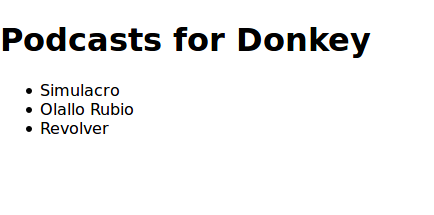
\includegraphics[scale=0.3]{react_first_app}
\end{figure}


\section*{Firebase para aplicaciones web}

Para utilizar los servicios Firebase en una aplicación web
se siguen los mismos pasos que para el caso de 
aplicaciones para Android. Desde la consola de Firebase
se crea el proyecto y se obtiene un fragmento de código
de inicialización. Ese código  contiene información de inicialización para configurar el SDK de Firebase JavaScript a fin de usar Authentication, Cloud Storage, Realtime Database y Cloud Firestore.


Se puede acceder
a cada servicio desde el espacio de nombres de \sphinxcode{\sphinxupquote{firebase}}:
\begin{itemize}
\item {} 
\sphinxcode{\sphinxupquote{firebase.auth()}} - Authentication

\item {} 
\sphinxcode{\sphinxupquote{firebase.storage()}} - Cloud Storage

\item {} 
\sphinxcode{\sphinxupquote{firebase.database()}} - Realtime Database

\item {} 
\sphinxcode{\sphinxupquote{firebase.firestore()}} - Cloud Firestore

\end{itemize}

El proceso para usar el servicio de Realtime Database y Authentication
es el mismo que en Android. Los métodos de lectura y escritura
se mantienen cambiando únicamente la sintaxis.


\subsection*{Firebase Realtime Database}
\label{\detokenize{firebase_web:firebase-realtime-database}}

Para leer la base de datos o escribir en ella, se necesita una instancia de
\sphinxcode{\sphinxupquote{firebase.database.Reference}}:

\fvset{hllines={, ,}}%
\begin{sphinxVerbatim}[commandchars=\\\{\}]
\PYG{o}{/}\PYG{o}{/} \PYG{n}{Obtiene} \PYG{n}{una} \PYG{n}{referencia} \PYG{n}{al} \PYG{n}{servicio} \PYG{n}{de} \PYG{n}{la} \PYG{n}{base} \PYG{n}{de} \PYG{n}{datos}
\PYG{n}{var} \PYG{n}{database} \PYG{o}{=} \PYG{n}{firebase}\PYG{o}{.}\PYG{n}{database}\PYG{p}{(}\PYG{p}{)}\PYG{p}{;}
\end{sphinxVerbatim}


\subsubsection*{Lectura y escritura de datos}
\label{\detokenize{firebase_web:lectura-y-escritura-de-datos}}
Para recuperar los datos de Firebase, se debe agregar un escuchador
asíncrono a \sphinxcode{\sphinxupquote{firebase.database.Reference}}. El escuchador se activa una vez para
el estado inicial de los datos y otra vez cuando los datos cambian.


Para ejecutar operaciones de escritura básicas, puedes usar \sphinxcode{\sphinxupquote{set()}} para guardar
datos en una referencia que especifiques y reemplazar los datos existentes en
esa ruta de acceso. Por ejemplo si se desea añadir un usuario a la base de datos,
una opción es la siguiente:

\fvset{hllines={, ,}}%
\begin{sphinxVerbatim}[commandchars=\\\{\}]
\PYG{n}{function} \PYG{n}{writeUserData}\PYG{p}{(}\PYG{n}{userId}\PYG{p}{,} \PYG{n}{name}\PYG{p}{,} \PYG{n}{email}\PYG{p}{,} \PYG{n}{imageUrl}\PYG{p}{)} \PYG{p}{\PYGZob{}}
\PYG{n}{firebase}\PYG{o}{.}\PYG{n}{database}\PYG{p}{(}\PYG{p}{)}\PYG{o}{.}\PYG{n}{ref}\PYG{p}{(}\PYG{l+s+s1}{\PYGZsq{}}\PYG{l+s+s1}{users/}\PYG{l+s+s1}{\PYGZsq{}} \PYG{o}{+} \PYG{n}{userId}\PYG{p}{)}\PYG{o}{.}\PYG{n}{set}\PYG{p}{(}\PYG{p}{\PYGZob{}}
    \PYG{n}{username}\PYG{p}{:} \PYG{n}{name}\PYG{p}{,}
    \PYG{n}{email}\PYG{p}{:} \PYG{n}{email}\PYG{p}{,}
    \PYG{n}{profile\PYGZus{}picture} \PYG{p}{:} \PYG{n}{imageUrl}
  \PYG{p}{\PYGZcb{}}\PYG{p}{)}\PYG{p}{;}
\PYG{p}{\PYGZcb{}}
\end{sphinxVerbatim}

\sphinxcode{\sphinxupquote{set()}} sobrescribe los datos en la ubicación que se especifica, incluidos
los nodos secundarios.


\subsubsection*{Detección de eventos en valores}
\label{\detokenize{firebase_web:detecta-eventos-en-valores}}
Si deseas leer datos de una ruta de acceso y escuchar para detectar cambios,
usa los métodos \sphinxcode{\sphinxupquote{on()}} o \sphinxcode{\sphinxupquote{once()}} de \sphinxcode{\sphinxupquote{firebase.database.Reference}}
para observar eventos.

El evento más común es \sphinxcode{\sphinxupquote{value}} y permite leer una instantánea estática del
contenido de una ruta de acceso determinada, en el estado en que se encontraba
en el momento del evento. Este método se activa cuando se vincula el escuchador
y se vuelve a activar cada vez que cambian los datos (incluidos los de
nivel secundario). La devolución de llamada del evento recibe una instantánea
que contiene todos los datos de dicha ubicación, incluidos los datos
secundarios. Si no hay datos, la instantánea tiene un valor nulo.

En el siguiente ejemplo se muestra una aplicación donde se recupera el valor
de un recurso en la base de datos:

\fvset{hllines={, ,}}%
\begin{sphinxVerbatim}[commandchars=\\\{\}]
\PYG{n}{var} \PYG{n}{resourceRef} \PYG{o}{=} \PYG{n}{firebase}\PYG{o}{.}\PYG{n}{database}\PYG{p}{(}\PYG{p}{)}\PYG{o}{.}\PYG{n}{ref}\PYG{p}{(}\PYG{l+s+s1}{\PYGZsq{}}\PYG{l+s+s1}{resource}\PYG{l+s+s1}{\PYGZsq{}}\PYG{p}{)}\PYG{p}{;}
\PYG{n}{resourceRef}\PYG{o}{.}\PYG{n}{on}\PYG{p}{(}\PYG{l+s+s1}{\PYGZsq{}}\PYG{l+s+s1}{value}\PYG{l+s+s1}{\PYGZsq{}}\PYG{p}{,} \PYG{n}{function}\PYG{p}{(}\PYG{n}{snapshot}\PYG{p}{)} \PYG{p}{\PYGZob{}}
  \PYG{n}{showValueOnScreen}\PYG{p}{(}\PYG{n}{snapshot}\PYG{o}{.}\PYG{n}{val}\PYG{p}{(}\PYG{p}{)}\PYG{p}{)}\PYG{p}{;}
\PYG{p}{\PYGZcb{}}\PYG{p}{)}\PYG{p}{;}
\end{sphinxVerbatim}

El escuchador recibe una \sphinxcode{\sphinxupquote{snapshot}} que contiene los datos de la ubicación
especifica en la base de datos en el momento del evento. Se pueden recuperar
los datos de la \sphinxcode{\sphinxupquote{snapshot}} con el método \sphinxcode{\sphinxupquote{val()}}.


\subsubsection{Actualizar o borrar datos}
\label{\detokenize{firebase_web:actualizar-o-borrar-datos}}
Para escribir de forma simultánea en elementos secundarios específicos de un
nodo sin sobrescribir otros nodos secundarios, usa el método \sphinxcode{\sphinxupquote{update()}}.

También existe el método \sphinxcode{\sphinxupquote{push()}} para añadir una entrada con un identificador
único sobre una referencia.

La forma más sencilla de borrar datos es llamar a \sphinxcode{\sphinxupquote{remove()}} en una referencia a
la ubicación de los datos. Para borrar, también puedes especificar nulo como
el valor de otra operación de escritura, como \sphinxcode{\sphinxupquote{set()}} o \sphinxcode{\sphinxupquote{update()}}.


\subsection*{Firebase Authentication}

De este servicio se utilizó la autenticación con
correo electrónico y contraseña.
El SDK de Firebase Authentication proporciona métodos para crear y administrar usuarios que utilizan sus direcciones de correo electrónico y sus contraseñas para acceder.

Para crear una cuenta de usuario nueva se pasa la dirección de correo electrónico y la contraseña del nuevo usuario a \texttt{createUserWithEmailAndPassword} para crear la cuenta nueva.

\fvset{hllines={, ,}}%
\begin{sphinxVerbatim}[commandchars=\\\{\}]
\PYG{n}{firebase}\PYG{o}{.}\PYG{n}{auth}\PYG{p}{(}\PYG{p}{)}\PYG{o}{.}\PYG{n}{createUserWithEmailAndPassword}\PYG{p}{(}\PYG{n}{email}\PYG{p}{,} \PYG{n}{password}\PYG{p}{)}\PYG{o}{.}\PYG{n}{catch}\PYG{p}{(}\PYG{n}{function}\PYG{p}{(}\PYG{n}{error}\PYG{p}{)} \PYG{p}{\PYGZob{}}
  \PYG{o}{/}\PYG{o}{/} \PYG{n}{El} \PYG{n}{manejo} \PYG{n}{de} \PYG{n}{errores} \PYG{n}{va} \PYG{n}{aquí}
  \PYG{n}{var} \PYG{n}{errorCode} \PYG{o}{=} \PYG{n}{error}\PYG{o}{.}\PYG{n}{code}\PYG{p}{;}
  \PYG{n}{var} \PYG{n}{errorMessage} \PYG{o}{=} \PYG{n}{error}\PYG{o}{.}\PYG{n}{message}\PYG{p}{;}
\PYG{p}{\PYGZcb{}}\PYG{p}{)}\PYG{p}{;}
\end{sphinxVerbatim}


Cuando un usuario accede a tus apps, se pasan la dirección de correo electrónico y la contraseña al método \texttt{signInWithEmailAndPassword}.

\fvset{hllines={, ,}}%
\begin{sphinxVerbatim}[commandchars=\\\{\}]
\PYG{n}{firebase}\PYG{o}{.}\PYG{n}{auth}\PYG{p}{(}\PYG{p}{)}\PYG{o}{.}\PYG{n}{signInWithEmailAndPassword}\PYG{p}{(}\PYG{n}{email}\PYG{p}{,} \PYG{n}{password}\PYG{p}{)}\PYG{o}{.}\PYG{n}{catch}\PYG{p}{(}\PYG{n}{function}\PYG{p}{(}\PYG{n}{error}\PYG{p}{)} \PYG{p}{\PYGZob{}}
\PYG{o}{/}\PYG{o}{/} \PYG{n}{Aquí} \PYG{n}{se} \PYG{n}{manejan} \PYG{n}{los} \PYG{n}{errores}
\PYG{n}{var} \PYG{n}{errorCode} \PYG{o}{=} \PYG{n}{error}\PYG{o}{.}\PYG{n}{code}\PYG{p}{;}
\PYG{n}{var} \PYG{n}{errorMessage} \PYG{o}{=} \PYG{n}{error}\PYG{o}{.}\PYG{n}{message}\PYG{p}{;}
\PYG{o}{/}\PYG{o}{/} \PYG{o}{.}\PYG{o}{.}\PYG{o}{.}
\PYG{p}{\PYGZcb{}}\PYG{p}{)}\PYG{p}{;}
\end{sphinxVerbatim}

La manera recomendada de obtener el usuario actual es establecer un observador en el objeto \sphinxcode{\sphinxupquote{Auth}}:

\fvset{hllines={, ,}}%
\begin{sphinxVerbatim}[commandchars=\\\{\}]
\PYG{n}{firebase}\PYG{o}{.}\PYG{n}{auth}\PYG{p}{(}\PYG{p}{)}\PYG{o}{.}\PYG{n}{onAuthStateChanged}\PYG{p}{(}\PYG{n}{function}\PYG{p}{(}\PYG{n}{user}\PYG{p}{)} \PYG{p}{\PYGZob{}}
\PYG{k}{if} \PYG{p}{(}\PYG{n}{user}\PYG{p}{)} \PYG{p}{\PYGZob{}}
  \PYG{o}{/}\PYG{o}{/} \PYG{n}{El} \PYG{n}{usuario} \PYG{n}{ha} \PYG{n}{iniciado} \PYG{n}{sesión}
\PYG{p}{\PYGZcb{}} \PYG{k}{else} \PYG{p}{\PYGZob{}}
  \PYG{o}{/}\PYG{o}{/} \PYG{n}{No} \PYG{n}{hay} \PYG{n}{un} \PYG{n}{usuario} \PYG{n}{activo}
\PYG{p}{\PYGZcb{}}
\PYG{p}{\PYGZcb{}}\PYG{p}{)}\PYG{p}{;}
\end{sphinxVerbatim}

También se puede usar la propiedad \sphinxcode{\sphinxupquote{currentUser}} para obtener el usuario que
accedió. Si un usuario no accedió a su cuenta, \sphinxcode{\sphinxupquote{currentUser}} mostrará un
resultado nulo:

\fvset{hllines={, ,}}%
\begin{sphinxVerbatim}[commandchars=\\\{\}]
\PYG{n}{var} \PYG{n}{user} \PYG{o}{=} \PYG{n}{firebase}\PYG{o}{.}\PYG{n}{auth}\PYG{p}{(}\PYG{p}{)}\PYG{o}{.}\PYG{n}{currentUser}\PYG{p}{;}
\PYG{k}{if} \PYG{p}{(}\PYG{n}{user}\PYG{p}{)} \PYG{p}{\PYGZob{}}
  \PYG{o}{/}\PYG{o}{/} \PYG{n}{El} \PYG{n}{usuario} \PYG{n}{ha} \PYG{n}{iniciado} \PYG{n}{sesión}
\PYG{p}{\PYGZcb{}} \PYG{k}{else} \PYG{p}{\PYGZob{}}
  \PYG{o}{/}\PYG{o}{/} \PYG{n}{No} \PYG{n}{hay} \PYG{n}{un} \PYG{n}{usuario} \PYG{n}{activo}
\PYG{p}{\PYGZcb{}}
\end{sphinxVerbatim}


Para obtener la información del perfil de un usuario, puedes usar las propiedades de una instancia de \texttt{User}. Por ejemplo:

\fvset{hllines={, ,}}%
\begin{sphinxVerbatim}[commandchars=\\\{\}]
\PYG{n}{var} \PYG{n}{user} \PYG{o}{=} \PYG{n}{firebase}\PYG{o}{.}\PYG{n}{auth}\PYG{p}{(}\PYG{p}{)}\PYG{o}{.}\PYG{n}{currentUser}\PYG{p}{;}
\PYG{n}{var} \PYG{n}{name}\PYG{p}{,} \PYG{n}{email}\PYG{p}{,} \PYG{n}{photoUrl}\PYG{p}{,} \PYG{n}{uid}\PYG{p}{,} \PYG{n}{emailVerified}\PYG{p}{;}

\PYG{k}{if} \PYG{p}{(}\PYG{n}{user} \PYG{o}{!=} \PYG{n}{null}\PYG{p}{)} \PYG{p}{\PYGZob{}}
  \PYG{n}{name} \PYG{o}{=} \PYG{n}{user}\PYG{o}{.}\PYG{n}{displayName}\PYG{p}{;}
  \PYG{n}{email} \PYG{o}{=} \PYG{n}{user}\PYG{o}{.}\PYG{n}{email}\PYG{p}{;}
  \PYG{n}{photoUrl} \PYG{o}{=} \PYG{n}{user}\PYG{o}{.}\PYG{n}{photoURL}\PYG{p}{;}
  \PYG{n}{emailVerified} \PYG{o}{=} \PYG{n}{user}\PYG{o}{.}\PYG{n}{emailVerified}\PYG{p}{;}
  \PYG{n}{uid} \PYG{o}{=} \PYG{n}{user}\PYG{o}{.}\PYG{n}{uid}\PYG{p}{;}  \PYG{o}{/}\PYG{o}{/} \PYG{n}{El} \PYG{n+nb}{id} \PYG{k}{del} \PYG{n}{usuario} \PYG{n}{es} \PYG{n}{único} \PYG{n}{en} \PYG{n}{un} \PYG{n}{proyecto} \PYG{n}{de} \PYG{n}{Firebase}

\PYG{p}{\PYGZcb{}}
\end{sphinxVerbatim}


Para salir de la sesión de un usuario, se llama a \sphinxcode{\sphinxupquote{signOut}}:

\fvset{hllines={, ,}}%
\begin{sphinxVerbatim}[commandchars=\\\{\}]
\PYG{n}{firebase}\PYG{o}{.}\PYG{n}{auth}\PYG{p}{(}\PYG{p}{)}\PYG{o}{.}\PYG{n}{signOut}\PYG{p}{(}\PYG{p}{)}\PYG{o}{.}\PYG{n}{then}\PYG{p}{(}\PYG{n}{function}\PYG{p}{(}\PYG{p}{)} \PYG{p}{\PYGZob{}}
\PYG{o}{/}\PYG{o}{/} \PYG{n}{Se} \PYG{n}{cierra} \PYG{n}{la} \PYG{n}{sesión} \PYG{n}{exitosamente}
\PYG{p}{\PYGZcb{}}\PYG{p}{)}\PYG{o}{.}\PYG{n}{catch}\PYG{p}{(}\PYG{n}{function}\PYG{p}{(}\PYG{n}{error}\PYG{p}{)} \PYG{p}{\PYGZob{}}
  \PYG{o}{/}\PYG{o}{/} \PYG{n}{Un} \PYG{n}{error} \PYG{n}{ocurrió}
\PYG{p}{\PYGZcb{}}\PYG{p}{)}\PYG{p}{;}
\end{sphinxVerbatim}


\subsection*{Firebase Hosting}
\label{\detokenize{firebase_web:firebase-hosting}}

Este servicio permite implementar y alojar los recursos estáticos de una aplicación
fácilmente (HTML, CSS, JavaScript, etc.). Todo el contenido se transmite a través
de HTTPS y está respaldado por una CDN global.

La ruta de implementación es la siguiente:

\begin{itemize}

\item{Instalar Firebase CLI.}
\label{\detokenize{firebase_web:instalar-firebase-cli}}
La CLI (interfaz de línea de comandos) de Firebase necesita Node.js y npm.

Para instalar Firebase CLI a través de npm se escribe los siguiente:

\fvset{hllines={, ,}}%
\begin{sphinxVerbatim}[commandchars=\\\{\}]
\PYG{n}{npm} \PYG{n}{install} \PYG{o}{\PYGZhy{}}\PYG{n}{g} \PYG{n}{firebase}\PYG{o}{\PYGZhy{}}\PYG{n}{tools}
\end{sphinxVerbatim}

Esto instala el comando \sphinxcode{\sphinxupquote{firebase}} de manera global.


\item\textbf{Inicializar la aplicación.}
\label{\detokenize{firebase_web:inicializar-la-aplicacion}}
Si se ejecuta el comando \sphinxcode{\sphinxupquote{firebase init}}, se crea un archivo de configuración
\sphinxcode{\sphinxupquote{firebase.json}} en la raíz del directorio del proyecto.


\item\textbf{Agregar un archivo.}
\label{\detokenize{firebase_web:agregar-un-archivo}}
Cuando se inicializa una aplicación, se pedirá proporcionar un directorio para
usarlo como raíz pública (el valor predeterminado es «public»). Si aún no
se tiene un archivo index.html válido en tu directorio raíz público, se creará
uno.


\item\textbf{Lanzar un sitio web.}
\label{\detokenize{firebase_web:implementar-un-sitio-web}}
Ejecutar \sphinxcode{\sphinxupquote{firebase deploy}} implementará la aplicación en el dominio
\sphinxcode{\sphinxupquote{\textless{}APP-DE-FIREBASE\textgreater{}.firebaseapp.com}}

\end{itemize}


\nocite{*}
\addcontentsline{toc}{chapter}{Bibliografía}
\bibliographystyle{unsrt}
\bibliography{referencias}

% \printbibliography

\end{document}